\documentclass[twoside]{book}

% Packages required by doxygen
\usepackage{fixltx2e}
\usepackage{calc}
\usepackage{doxygen}
\usepackage[export]{adjustbox} % also loads graphicx
\usepackage{graphicx}
\usepackage[utf8]{inputenc}
\usepackage{makeidx}
\usepackage{multicol}
\usepackage{multirow}
\PassOptionsToPackage{warn}{textcomp}
\usepackage{textcomp}
\usepackage[nointegrals]{wasysym}
\usepackage[table]{xcolor}

% Font selection
\usepackage[T1]{fontenc}
\usepackage[scaled=.90]{helvet}
\usepackage{courier}
\usepackage{amssymb}
\usepackage{sectsty}
\renewcommand{\familydefault}{\sfdefault}
\allsectionsfont{%
  \fontseries{bc}\selectfont%
  \color{darkgray}%
}
\renewcommand{\DoxyLabelFont}{%
  \fontseries{bc}\selectfont%
  \color{darkgray}%
}
\newcommand{\+}{\discretionary{\mbox{\scriptsize$\hookleftarrow$}}{}{}}

% Page & text layout
\usepackage{geometry}
\geometry{%
  a4paper,%
  top=2.5cm,%
  bottom=2.5cm,%
  left=2.5cm,%
  right=2.5cm%
}
\tolerance=750
\hfuzz=15pt
\hbadness=750
\setlength{\emergencystretch}{15pt}
\setlength{\parindent}{0cm}
\setlength{\parskip}{3ex plus 2ex minus 2ex}
\makeatletter
\renewcommand{\paragraph}{%
  \@startsection{paragraph}{4}{0ex}{-1.0ex}{1.0ex}{%
    \normalfont\normalsize\bfseries\SS@parafont%
  }%
}
\renewcommand{\subparagraph}{%
  \@startsection{subparagraph}{5}{0ex}{-1.0ex}{1.0ex}{%
    \normalfont\normalsize\bfseries\SS@subparafont%
  }%
}
\makeatother

% Headers & footers
\usepackage{fancyhdr}
\pagestyle{fancyplain}
\fancyhead[LE]{\fancyplain{}{\bfseries\thepage}}
\fancyhead[CE]{\fancyplain{}{}}
\fancyhead[RE]{\fancyplain{}{\bfseries\leftmark}}
\fancyhead[LO]{\fancyplain{}{\bfseries\rightmark}}
\fancyhead[CO]{\fancyplain{}{}}
\fancyhead[RO]{\fancyplain{}{\bfseries\thepage}}
\fancyfoot[LE]{\fancyplain{}{}}
\fancyfoot[CE]{\fancyplain{}{}}
\fancyfoot[RE]{\fancyplain{}{\bfseries\scriptsize Generated by Doxygen }}
\fancyfoot[LO]{\fancyplain{}{\bfseries\scriptsize Generated by Doxygen }}
\fancyfoot[CO]{\fancyplain{}{}}
\fancyfoot[RO]{\fancyplain{}{}}
\renewcommand{\footrulewidth}{0.4pt}
\renewcommand{\chaptermark}[1]{%
  \markboth{#1}{}%
}
\renewcommand{\sectionmark}[1]{%
  \markright{\thesection\ #1}%
}

% Indices & bibliography
\usepackage{natbib}
\usepackage[titles]{tocloft}
\setcounter{tocdepth}{3}
\setcounter{secnumdepth}{5}
\makeindex

% Hyperlinks (required, but should be loaded last)
\usepackage{ifpdf}
\ifpdf
  \usepackage[pdftex,pagebackref=true]{hyperref}
\else
  \usepackage[ps2pdf,pagebackref=true]{hyperref}
\fi
\hypersetup{%
  colorlinks=true,%
  linkcolor=blue,%
  citecolor=blue,%
  unicode%
}

% Custom commands
\newcommand{\clearemptydoublepage}{%
  \newpage{\pagestyle{empty}\cleardoublepage}%
}

\usepackage{caption}
\captionsetup{labelsep=space,justification=centering,font={bf},singlelinecheck=off,skip=4pt,position=top}

%===== C O N T E N T S =====

\begin{document}

% Titlepage & ToC
\hypersetup{pageanchor=false,
             bookmarksnumbered=true,
             pdfencoding=unicode
            }
\pagenumbering{alph}
\begin{titlepage}
\vspace*{7cm}
\begin{center}%
{\Large lray \\[1ex]\large 0.\+1 }\\
\vspace*{1cm}
{\large Generated by Doxygen 1.8.13}\\
\end{center}
\end{titlepage}
\clearemptydoublepage
\pagenumbering{roman}
\tableofcontents
\clearemptydoublepage
\pagenumbering{arabic}
\hypersetup{pageanchor=true}

%--- Begin generated contents ---
\chapter{L\+R\+AY program}
\label{md_readme}
\Hypertarget{md_readme}
\section*{Lray}

usage\+: lray -\/n \mbox{[}1$\vert$2$\vert$3\mbox{]} \mbox{[}-\/ps NB if n=3\mbox{]} -\/i $<$my\+\_\+scene.\+xml$>$ \mbox{[}-\/o $<$image name$>$=\char`\"{}\char`\"{}$>$\mbox{]} \mbox{[}-\/t timer the scene calculation\mbox{]}~\newline
 help \+: lray show a scene specified by a a xml file~\newline
 Options \+: -\/n nb -\/$>$ the level of scene ~\newline
 1\+: single ray tracing ~\newline
 2\+: interactive ray tracing ~\newline
 3\+: recursive interactive ray tracing

-\/ps nb -\/$>$ pixel sampling number of rays launched per pixel

-\/i scene.\+xml the scene to input

-\/o output\+\_\+image (optional for -\/n = 2 or 3) export the scene in a png image without print it in a window

-\/t timer the scene calculation

\section*{Generator}

usage \+: Usage\+: generator width height \mbox{[}-\/p specify objects to generate e.\+g -\/p cube,cylindre,rectangle,sphere,triangle\mbox{]} -\/n nb\+\_\+object -\/o output\+\_\+file~\newline
 utiliser l\textquotesingle{}option -\/p seulement si on veut spécifier les objets à générer~\newline
 l\textquotesingle{}option -\/a ou l\textquotesingle{}absence de l\textquotesingle{}option p permet de dire que l\textquotesingle{}on souhaite tous les types d\textquotesingle{}objets

\section*{I\+N\+TÉ\+R\+A\+C\+T\+I\+ON U\+T\+I\+L\+I\+S\+A\+T\+E\+UR}

commandes\+:
\begin{DoxyItemize}
\item déplacer la caméra vers la gauche ou vers la droite avec les touches K et M respectivement (des rotations autour de l’axe oy). ~\newline

\item déplacer la caméra vers le haut ou vers le bas avec les touches O et L respectivement (des rotations autour de l’axe ox). ~\newline

\item zoomer ou dézoomer avec les touches P et I respectivement (des translations). ~\newline

\item activer ou désactiver le rendu progressif (régulier avec 9 rayons) avec un bouton sur la fenêtre. ~\newline

\item ajouter (resp. enlever) des réflexions spéculaires pures avec la touche +/= (resp. -\/). ~\newline

\item la touche S permet de sauvegarder la scène courante. ~\newline

\end{DoxyItemize}

\section*{Install.\+sh}

install.\+sh permet d\textquotesingle{}installer la librairie g3x sur le pc 
\chapter{Data Structure Index}
\section{Data Structures}
Here are the data structures with brief descriptions\+:\begin{DoxyCompactList}
\item\contentsline{section}{\hyperlink{struct__lst__obj}{\+\_\+lst\+\_\+obj} }{\pageref{struct__lst__obj}}{}
\item\contentsline{section}{\hyperlink{struct__lst__point}{\+\_\+lst\+\_\+point} }{\pageref{struct__lst__point}}{}
\item\contentsline{section}{\hyperlink{struct__object}{\+\_\+object} }{\pageref{struct__object}}{}
\item\contentsline{section}{\hyperlink{struct_camera}{Camera} \\*\hyperlink{struct_camera}{Camera} observing the scene }{\pageref{struct_camera}}{}
\item\contentsline{section}{\hyperlink{struct_color}{Color} \\*R\+GB color }{\pageref{struct_color}}{}
\item\contentsline{section}{\hyperlink{struct_cube}{Cube} \\*\hyperlink{struct_cube}{Cube} }{\pageref{struct_cube}}{}
\item\contentsline{section}{\hyperlink{struct_cylindre}{Cylindre} \\*Cylinder }{\pageref{struct_cylindre}}{}
\item\contentsline{section}{\hyperlink{struct_g3_xadres}{G3\+Xadres} }{\pageref{struct_g3_xadres}}{}
\item\contentsline{section}{\hyperlink{struct_g3_xbut}{G3\+Xbut} }{\pageref{struct_g3_xbut}}{}
\item\contentsline{section}{\hyperlink{struct_g3_xcamera}{G3\+Xcamera} }{\pageref{struct_g3_xcamera}}{}
\item\contentsline{section}{\hyperlink{struct_g3_xclock}{G3\+Xclock} }{\pageref{struct_g3_xclock}}{}
\item\contentsline{section}{\hyperlink{struct_g3_ximgnames}{G3\+Ximgnames} }{\pageref{struct_g3_ximgnames}}{}
\item\contentsline{section}{\hyperlink{struct_g3_xkey}{G3\+Xkey} }{\pageref{struct_g3_xkey}}{}
\item\contentsline{section}{\hyperlink{struct_g3_xlight}{G3\+Xlight} }{\pageref{struct_g3_xlight}}{}
\item\contentsline{section}{\hyperlink{struct_g3_xparam}{G3\+Xparam} }{\pageref{struct_g3_xparam}}{}
\item\contentsline{section}{\hyperlink{struct_g3_xpnm}{G3\+Xpnm} }{\pageref{struct_g3_xpnm}}{}
\item\contentsline{section}{\hyperlink{struct_g3_xpopup}{G3\+Xpopup} }{\pageref{struct_g3_xpopup}}{}
\item\contentsline{section}{\hyperlink{struct_g3_xprm}{G3\+Xprm} }{\pageref{struct_g3_xprm}}{}
\item\contentsline{section}{\hyperlink{struct_g3_xquat}{G3\+Xquat} }{\pageref{struct_g3_xquat}}{}
\item\contentsline{section}{\hyperlink{struct_g3_xscroll}{G3\+Xscroll} }{\pageref{struct_g3_xscroll}}{}
\item\contentsline{section}{\hyperlink{struct_g3_xswitch}{G3\+Xswitch} }{\pageref{struct_g3_xswitch}}{}
\item\contentsline{section}{\hyperlink{struct_image}{Image} \\*\hyperlink{struct_image}{Image} }{\pageref{struct_image}}{}
\item\contentsline{section}{\hyperlink{structlst__obj}{lst\+\_\+obj} \\*List of objects to generate }{\pageref{structlst__obj}}{}
\item\contentsline{section}{\hyperlink{structlst___object}{lst\+\_\+\+Object} \\*List of objects }{\pageref{structlst___object}}{}
\item\contentsline{section}{\hyperlink{structlst___source}{lst\+\_\+\+Source} \\*Liste of light sources }{\pageref{structlst___source}}{}
\item\contentsline{section}{\hyperlink{struct_object}{Object} \\*\hyperlink{struct_object}{Object} }{\pageref{struct_object}}{}
\item\contentsline{section}{\hyperlink{struct_option}{Option} \\*Options specified by the user }{\pageref{struct_option}}{}
\item\contentsline{section}{\hyperlink{structpng__t}{png\+\_\+t} \\*Type representing a png image }{\pageref{structpng__t}}{}
\item\contentsline{section}{\hyperlink{struct_point}{Point} \\*\hyperlink{struct_point}{Point} in 3D space }{\pageref{struct_point}}{}
\item\contentsline{section}{\hyperlink{struct_rectangle}{Rectangle} \\*\hyperlink{struct_rectangle}{Rectangle} }{\pageref{struct_rectangle}}{}
\item\contentsline{section}{\hyperlink{struct_scene}{Scene} \\*3D scene seen by the camera }{\pageref{struct_scene}}{}
\item\contentsline{section}{\hyperlink{struct_scene__info}{Scene\+\_\+info} \\*All parameters desired by the user when generating the scene }{\pageref{struct_scene__info}}{}
\item\contentsline{section}{\hyperlink{struct_source}{Source} \\*Light source }{\pageref{struct_source}}{}
\item\contentsline{section}{\hyperlink{struct_sphere}{Sphere} \\*\hyperlink{struct_sphere}{Sphere} }{\pageref{struct_sphere}}{}
\item\contentsline{section}{\hyperlink{struct_triangle}{Triangle} \\*\hyperlink{struct_triangle}{Triangle} }{\pageref{struct_triangle}}{}
\item\contentsline{section}{\hyperlink{struct_vecteur}{Vecteur} \\*Vector in 3D space }{\pageref{struct_vecteur}}{}
\end{DoxyCompactList}

\chapter{File Index}
\section{File List}
Here is a list of all files with brief descriptions\+:\begin{DoxyCompactList}
\item\contentsline{section}{\hyperlink{_scene__generator_8c}{Scene\+\_\+generator.\+c} }{\pageref{_scene__generator_8c}}{}
\item\contentsline{section}{include/\hyperlink{_camera_8h}{Camera.\+h} \\*\hyperlink{struct_camera}{Camera} filming the scene }{\pageref{_camera_8h}}{}
\item\contentsline{section}{include/\hyperlink{_color_8h}{Color.\+h} \\*R\+GB color type and all functions related to it }{\pageref{_color_8h}}{}
\item\contentsline{section}{include/\hyperlink{_cube_8h}{Cube.\+h} \\*\hyperlink{struct_cube}{Cube} type and functions related to it }{\pageref{_cube_8h}}{}
\item\contentsline{section}{include/\hyperlink{_cylindre_8h}{Cylindre.\+h} \\*Cylinder }{\pageref{_cylindre_8h}}{}
\item\contentsline{section}{include/\hyperlink{_hmat_8h}{Hmat.\+h} \\*Type Hmat representing homogeneous matrices and functions related to if }{\pageref{_hmat_8h}}{}
\item\contentsline{section}{include/\hyperlink{_image_8h}{Image.\+h} \\*R\+GB image }{\pageref{_image_8h}}{}
\item\contentsline{section}{include/\hyperlink{_light_8h}{Light.\+h} }{\pageref{_light_8h}}{}
\item\contentsline{section}{include/\hyperlink{_lst___object_8h}{Lst\+\_\+\+Object.\+h} \\*List of Objects (shapes) }{\pageref{_lst___object_8h}}{}
\item\contentsline{section}{include/\hyperlink{_object_8h}{Object.\+h} }{\pageref{_object_8h}}{}
\item\contentsline{section}{include/\hyperlink{_option_8h}{Option.\+h} \\*Options specified by the user when launching the program }{\pageref{_option_8h}}{}
\item\contentsline{section}{include/\hyperlink{_parser_8h}{Parser.\+h} \\*Parser of user command line and a scene parser }{\pageref{_parser_8h}}{}
\item\contentsline{section}{include/\hyperlink{_png___output_8h}{Png\+\_\+\+Output.\+h} \\*Export a \hyperlink{struct_image}{Image} in png }{\pageref{_png___output_8h}}{}
\item\contentsline{section}{include/\hyperlink{_point_8h}{Point.\+h} \\*\hyperlink{struct_point}{Point} type in a 3D space and all functions related to this type }{\pageref{_point_8h}}{}
\item\contentsline{section}{include/\hyperlink{_rectangle_8h}{Rectangle.\+h} \\*Light type }{\pageref{_rectangle_8h}}{}
\item\contentsline{section}{include/\hyperlink{_scene_8h}{Scene.\+h} \\*\hyperlink{struct_scene}{Scene} }{\pageref{_scene_8h}}{}
\item\contentsline{section}{include/\hyperlink{_sphere_8h}{Sphere.\+h} \\*\hyperlink{struct_sphere}{Sphere} }{\pageref{_sphere_8h}}{}
\item\contentsline{section}{include/\hyperlink{_triangle_8h}{Triangle.\+h} \\*\hyperlink{struct_triangle}{Triangle} }{\pageref{_triangle_8h}}{}
\item\contentsline{section}{include/\hyperlink{_vecteur_8h}{Vecteur.\+h} \\*Vector type in a 3D space and all functions related to this type }{\pageref{_vecteur_8h}}{}
\item\contentsline{section}{include/\hyperlink{_window_8h}{Window.\+h} \\*Window to display a scene }{\pageref{_window_8h}}{}
\item\contentsline{section}{libg3x/include/\hyperlink{g3x_8h}{g3x.\+h} }{\pageref{g3x_8h}}{}
\item\contentsline{section}{libg3x/include/\hyperlink{g3x__capture_8h}{g3x\+\_\+capture.\+h} }{\pageref{g3x__capture_8h}}{}
\item\contentsline{section}{libg3x/include/\hyperlink{g3x__colors_8h}{g3x\+\_\+colors.\+h} }{\pageref{g3x__colors_8h}}{}
\item\contentsline{section}{libg3x/include/\hyperlink{g3x___g_ltransfo_8h}{g3x\+\_\+\+G\+Ltransfo.\+h} }{\pageref{g3x___g_ltransfo_8h}}{}
\item\contentsline{section}{libg3x/include/\hyperlink{g3x__macros_8h}{g3x\+\_\+macros.\+h} }{\pageref{g3x__macros_8h}}{}
\item\contentsline{section}{libg3x/include/\hyperlink{g3x__pnm_8h}{g3x\+\_\+pnm.\+h} }{\pageref{g3x__pnm_8h}}{}
\item\contentsline{section}{libg3x/include/\hyperlink{g3x__quaternions_8h}{g3x\+\_\+quaternions.\+h} }{\pageref{g3x__quaternions_8h}}{}
\item\contentsline{section}{libg3x/include/\hyperlink{g3x__tools_8h}{g3x\+\_\+tools.\+h} }{\pageref{g3x__tools_8h}}{}
\item\contentsline{section}{libg3x/include/\hyperlink{g3x__transfo_8h}{g3x\+\_\+transfo.\+h} }{\pageref{g3x__transfo_8h}}{}
\item\contentsline{section}{libg3x/include/\hyperlink{g3x__types_8h}{g3x\+\_\+types.\+h} }{\pageref{g3x__types_8h}}{}
\item\contentsline{section}{libg3x/include/\hyperlink{g3x__window_8h}{g3x\+\_\+window.\+h} }{\pageref{g3x__window_8h}}{}
\item\contentsline{section}{libg3x/include/\hyperlink{mtracer_8h}{mtracer.\+h} }{\pageref{mtracer_8h}}{}
\item\contentsline{section}{libg3x/src/\hyperlink{3_ddemo_8c}{3\+Ddemo.\+c} }{\pageref{3_ddemo_8c}}{}
\item\contentsline{section}{libg3x/src/\hyperlink{g3x__button_8c}{g3x\+\_\+button.\+c} }{\pageref{g3x__button_8c}}{}
\item\contentsline{section}{libg3x/src/\hyperlink{g3x__camlight_8c}{g3x\+\_\+camlight.\+c} }{\pageref{g3x__camlight_8c}}{}
\item\contentsline{section}{libg3x/src/\hyperlink{g3x__capture_8c}{g3x\+\_\+capture.\+c} }{\pageref{g3x__capture_8c}}{}
\item\contentsline{section}{libg3x/src/\hyperlink{g3x__ctrlprm_8c}{g3x\+\_\+ctrlprm.\+c} }{\pageref{g3x__ctrlprm_8c}}{}
\item\contentsline{section}{libg3x/src/\hyperlink{g3x___g_ltransfo_8c}{g3x\+\_\+\+G\+Ltransfo.\+c} }{\pageref{g3x___g_ltransfo_8c}}{}
\item\contentsline{section}{libg3x/src/\hyperlink{g3x__keys_8c}{g3x\+\_\+keys.\+c} }{\pageref{g3x__keys_8c}}{}
\item\contentsline{section}{libg3x/src/\hyperlink{g3x__octree_8c}{g3x\+\_\+octree.\+c} }{\pageref{g3x__octree_8c}}{}
\item\contentsline{section}{libg3x/src/\hyperlink{g3x__pnm_8c}{g3x\+\_\+pnm.\+c} }{\pageref{g3x__pnm_8c}}{}
\item\contentsline{section}{libg3x/src/\hyperlink{g3x__popup_8c}{g3x\+\_\+popup.\+c} }{\pageref{g3x__popup_8c}}{}
\item\contentsline{section}{libg3x/src/\hyperlink{g3x__quaternions_8c}{g3x\+\_\+quaternions.\+c} }{\pageref{g3x__quaternions_8c}}{}
\item\contentsline{section}{libg3x/src/\hyperlink{g3x__scroll_8c}{g3x\+\_\+scroll.\+c} }{\pageref{g3x__scroll_8c}}{}
\item\contentsline{section}{libg3x/src/\hyperlink{g3x__switch_8c}{g3x\+\_\+switch.\+c} }{\pageref{g3x__switch_8c}}{}
\item\contentsline{section}{libg3x/src/\hyperlink{g3x__tools_8c}{g3x\+\_\+tools.\+c} }{\pageref{g3x__tools_8c}}{}
\item\contentsline{section}{libg3x/src/\hyperlink{g3x__transfo_8c}{g3x\+\_\+transfo.\+c} }{\pageref{g3x__transfo_8c}}{}
\item\contentsline{section}{libg3x/src/\hyperlink{g3x__window_8c}{g3x\+\_\+window.\+c} }{\pageref{g3x__window_8c}}{}
\item\contentsline{section}{src/\hyperlink{_camera_8c}{Camera.\+c} }{\pageref{_camera_8c}}{}
\item\contentsline{section}{src/\hyperlink{_color_8c}{Color.\+c} }{\pageref{_color_8c}}{}
\item\contentsline{section}{src/\hyperlink{_cube_8c}{Cube.\+c} }{\pageref{_cube_8c}}{}
\item\contentsline{section}{src/\hyperlink{_cylindre_8c}{Cylindre.\+c} }{\pageref{_cylindre_8c}}{}
\item\contentsline{section}{src/\hyperlink{_hmat_8c}{Hmat.\+c} }{\pageref{_hmat_8c}}{}
\item\contentsline{section}{src/\hyperlink{_image_8c}{Image.\+c} }{\pageref{_image_8c}}{}
\item\contentsline{section}{src/\hyperlink{_light_8c}{Light.\+c} }{\pageref{_light_8c}}{}
\item\contentsline{section}{src/\hyperlink{_lst___object_8c}{Lst\+\_\+\+Object.\+c} }{\pageref{_lst___object_8c}}{}
\item\contentsline{section}{src/\hyperlink{main_8c}{main.\+c} }{\pageref{main_8c}}{}
\item\contentsline{section}{src/\hyperlink{_object_8c}{Object.\+c} }{\pageref{_object_8c}}{}
\item\contentsline{section}{src/\hyperlink{_option_8c}{Option.\+c} }{\pageref{_option_8c}}{}
\item\contentsline{section}{src/\hyperlink{_parser_8c}{Parser.\+c} }{\pageref{_parser_8c}}{}
\item\contentsline{section}{src/\hyperlink{_png___output_8c}{Png\+\_\+\+Output.\+c} }{\pageref{_png___output_8c}}{}
\item\contentsline{section}{src/\hyperlink{_point_8c}{Point.\+c} }{\pageref{_point_8c}}{}
\item\contentsline{section}{src/\hyperlink{_rectangle_8c}{Rectangle.\+c} }{\pageref{_rectangle_8c}}{}
\item\contentsline{section}{src/\hyperlink{_scene_8c}{Scene.\+c} }{\pageref{_scene_8c}}{}
\item\contentsline{section}{src/\hyperlink{_sphere_8c}{Sphere.\+c} }{\pageref{_sphere_8c}}{}
\item\contentsline{section}{src/\hyperlink{_triangle_8c}{Triangle.\+c} }{\pageref{_triangle_8c}}{}
\item\contentsline{section}{src/\hyperlink{_vecteur_8c}{Vecteur.\+c} }{\pageref{_vecteur_8c}}{}
\item\contentsline{section}{src/\hyperlink{_window_8c}{Window.\+c} }{\pageref{_window_8c}}{}
\end{DoxyCompactList}

\chapter{Data Structure Documentation}
\hypertarget{struct__lst__obj}{}\section{\+\_\+lst\+\_\+obj Struct Reference}
\label{struct__lst__obj}\index{\+\_\+lst\+\_\+obj@{\+\_\+lst\+\_\+obj}}


{\ttfamily \#include $<$Lst\+\_\+\+Object.\+h$>$}



Collaboration diagram for \+\_\+lst\+\_\+obj\+:\nopagebreak
\begin{figure}[H]
\begin{center}
\leavevmode
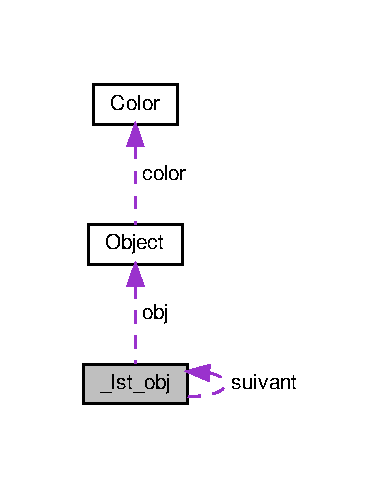
\includegraphics[width=183pt]{struct__lst__obj__coll__graph}
\end{center}
\end{figure}
\subsection*{Data Fields}
\begin{DoxyCompactItemize}
\item 
\hyperlink{struct_object}{Object} \hyperlink{struct__lst__obj_a3a6f22968f6ad522baa85c809b856bae}{obj}
\item 
struct \hyperlink{struct__lst__obj}{\+\_\+lst\+\_\+obj} $\ast$ \hyperlink{struct__lst__obj_a30057e853c9335659e7e45f3052ca333}{suivant}
\end{DoxyCompactItemize}


\subsection{Field Documentation}
\mbox{\Hypertarget{struct__lst__obj_a3a6f22968f6ad522baa85c809b856bae}\label{struct__lst__obj_a3a6f22968f6ad522baa85c809b856bae}} 
\index{\+\_\+lst\+\_\+obj@{\+\_\+lst\+\_\+obj}!obj@{obj}}
\index{obj@{obj}!\+\_\+lst\+\_\+obj@{\+\_\+lst\+\_\+obj}}
\subsubsection{\texorpdfstring{obj}{obj}}
{\footnotesize\ttfamily \hyperlink{struct_object}{Object} obj}

the object of the current node \mbox{\Hypertarget{struct__lst__obj_a30057e853c9335659e7e45f3052ca333}\label{struct__lst__obj_a30057e853c9335659e7e45f3052ca333}} 
\index{\+\_\+lst\+\_\+obj@{\+\_\+lst\+\_\+obj}!suivant@{suivant}}
\index{suivant@{suivant}!\+\_\+lst\+\_\+obj@{\+\_\+lst\+\_\+obj}}
\subsubsection{\texorpdfstring{suivant}{suivant}}
{\footnotesize\ttfamily struct \hyperlink{struct__lst__obj}{\+\_\+lst\+\_\+obj}$\ast$ suivant}

pointer to a next node 

The documentation for this struct was generated from the following file\+:\begin{DoxyCompactItemize}
\item 
include/\hyperlink{_lst___object_8h}{Lst\+\_\+\+Object.\+h}\end{DoxyCompactItemize}

\hypertarget{struct__lst__point}{}\section{\+\_\+lst\+\_\+point Struct Reference}
\label{struct__lst__point}\index{\+\_\+lst\+\_\+point@{\+\_\+lst\+\_\+point}}


{\ttfamily \#include $<$Light.\+h$>$}



Collaboration diagram for \+\_\+lst\+\_\+point\+:\nopagebreak
\begin{figure}[H]
\begin{center}
\leavevmode
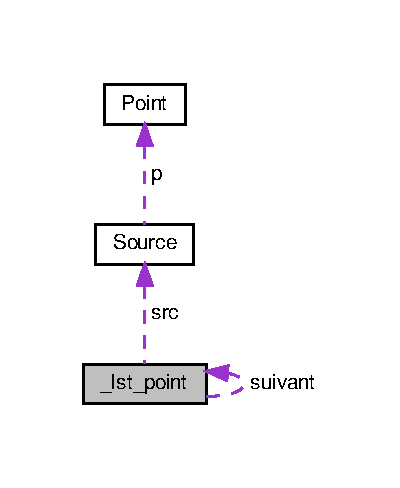
\includegraphics[width=192pt]{struct__lst__point__coll__graph}
\end{center}
\end{figure}
\subsection*{Data Fields}
\begin{DoxyCompactItemize}
\item 
\hyperlink{struct_source}{Source} \hyperlink{struct__lst__point_a6626a7de24e24cfe4e4464ad9743b2e3}{src}
\item 
struct \hyperlink{struct__lst__point}{\+\_\+lst\+\_\+point} $\ast$ \hyperlink{struct__lst__point_a762f437c3be21ea03bd41426932c4547}{suivant}
\end{DoxyCompactItemize}


\subsection{Field Documentation}
\mbox{\Hypertarget{struct__lst__point_a6626a7de24e24cfe4e4464ad9743b2e3}\label{struct__lst__point_a6626a7de24e24cfe4e4464ad9743b2e3}} 
\index{\+\_\+lst\+\_\+point@{\+\_\+lst\+\_\+point}!src@{src}}
\index{src@{src}!\+\_\+lst\+\_\+point@{\+\_\+lst\+\_\+point}}
\subsubsection{\texorpdfstring{src}{src}}
{\footnotesize\ttfamily \hyperlink{struct_source}{Source} src}

the source of the current node \mbox{\Hypertarget{struct__lst__point_a762f437c3be21ea03bd41426932c4547}\label{struct__lst__point_a762f437c3be21ea03bd41426932c4547}} 
\index{\+\_\+lst\+\_\+point@{\+\_\+lst\+\_\+point}!suivant@{suivant}}
\index{suivant@{suivant}!\+\_\+lst\+\_\+point@{\+\_\+lst\+\_\+point}}
\subsubsection{\texorpdfstring{suivant}{suivant}}
{\footnotesize\ttfamily struct \hyperlink{struct__lst__point}{\+\_\+lst\+\_\+point}$\ast$ suivant}

pointer to a next node 

The documentation for this struct was generated from the following file\+:\begin{DoxyCompactItemize}
\item 
include/\hyperlink{_light_8h}{Light.\+h}\end{DoxyCompactItemize}

\hypertarget{struct__object}{}\section{\+\_\+object Struct Reference}
\label{struct__object}\index{\+\_\+object@{\+\_\+object}}


Collaboration diagram for \+\_\+object\+:\nopagebreak
\begin{figure}[H]
\begin{center}
\leavevmode
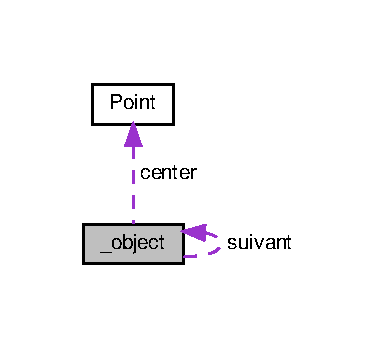
\includegraphics[width=181pt]{struct__object__coll__graph}
\end{center}
\end{figure}
\subsection*{Data Fields}
\begin{DoxyCompactItemize}
\item 
int \hyperlink{struct__object_a395279899207ce7f17adf9fdb8ee97ee}{radius}
\item 
\hyperlink{struct_point}{Point} \hyperlink{struct__object_a24bb1c337bce91dd3e7a4a4372b11793}{center}
\item 
struct \hyperlink{struct__object}{\+\_\+object} $\ast$ \hyperlink{struct__object_afb085435a094e9028d6ab3915166b2f3}{suivant}
\end{DoxyCompactItemize}


\subsection{Field Documentation}
\mbox{\Hypertarget{struct__object_a24bb1c337bce91dd3e7a4a4372b11793}\label{struct__object_a24bb1c337bce91dd3e7a4a4372b11793}} 
\index{\+\_\+object@{\+\_\+object}!center@{center}}
\index{center@{center}!\+\_\+object@{\+\_\+object}}
\subsubsection{\texorpdfstring{center}{center}}
{\footnotesize\ttfamily \hyperlink{struct_point}{Point} center}

the center \mbox{\Hypertarget{struct__object_a395279899207ce7f17adf9fdb8ee97ee}\label{struct__object_a395279899207ce7f17adf9fdb8ee97ee}} 
\index{\+\_\+object@{\+\_\+object}!radius@{radius}}
\index{radius@{radius}!\+\_\+object@{\+\_\+object}}
\subsubsection{\texorpdfstring{radius}{radius}}
{\footnotesize\ttfamily int radius}

the radius of the object \mbox{\Hypertarget{struct__object_afb085435a094e9028d6ab3915166b2f3}\label{struct__object_afb085435a094e9028d6ab3915166b2f3}} 
\index{\+\_\+object@{\+\_\+object}!suivant@{suivant}}
\index{suivant@{suivant}!\+\_\+object@{\+\_\+object}}
\subsubsection{\texorpdfstring{suivant}{suivant}}
{\footnotesize\ttfamily struct \hyperlink{struct__object}{\+\_\+object}$\ast$ suivant}

pointer to the next node 

The documentation for this struct was generated from the following file\+:\begin{DoxyCompactItemize}
\item 
\hyperlink{_scene__generator_8c}{Scene\+\_\+generator.\+c}\end{DoxyCompactItemize}

\hypertarget{struct_camera}{}\section{Camera Struct Reference}
\label{struct_camera}\index{Camera@{Camera}}


represents a camera observing the scene  




{\ttfamily \#include $<$Camera.\+h$>$}



Collaboration diagram for Camera\+:\nopagebreak
\begin{figure}[H]
\begin{center}
\leavevmode
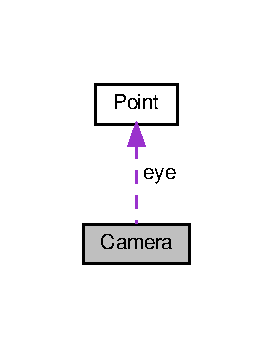
\includegraphics[width=131pt]{struct_camera__coll__graph}
\end{center}
\end{figure}
\subsection*{Data Fields}
\begin{DoxyCompactItemize}
\item 
\hyperlink{struct_point}{Point} \hyperlink{struct_camera_a3f0f7501902ff66889e21c369d1159d0}{eye}
\item 
int \hyperlink{struct_camera_a5496c6b1391a3368a05f6b7a44cc2aa0}{resolution} \mbox{[}2\mbox{]}
\item 
\hyperlink{g3x__transfo_8h_a89b2b23e407882a535d835574a7912e1}{double} \hyperlink{struct_camera_aad384fcdec994533787d54acd096c5cb}{screen} \mbox{[}2\mbox{]}
\item 
\hyperlink{_hmat_8h_a7263a9d077d77f58425e01446b766c9f}{Hmat} \hyperlink{struct_camera_a94d9bf45fca18b32481a1bbd1ea58bdf}{M}
\end{DoxyCompactItemize}


\subsection{Detailed Description}
represents a camera observing the scene 

represents a camera observing the scene 

\subsection{Field Documentation}
\mbox{\Hypertarget{struct_camera_a3f0f7501902ff66889e21c369d1159d0}\label{struct_camera_a3f0f7501902ff66889e21c369d1159d0}} 
\index{Camera@{Camera}!eye@{eye}}
\index{eye@{eye}!Camera@{Camera}}
\subsubsection{\texorpdfstring{eye}{eye}}
{\footnotesize\ttfamily \hyperlink{struct_point}{Point} eye}

the eye of the camera observing the scene \mbox{\Hypertarget{struct_camera_a94d9bf45fca18b32481a1bbd1ea58bdf}\label{struct_camera_a94d9bf45fca18b32481a1bbd1ea58bdf}} 
\index{Camera@{Camera}!M@{M}}
\index{M@{M}!Camera@{Camera}}
\subsubsection{\texorpdfstring{M}{M}}
{\footnotesize\ttfamily \hyperlink{_hmat_8h_a7263a9d077d77f58425e01446b766c9f}{Hmat} M}

\mbox{\Hypertarget{struct_camera_a5496c6b1391a3368a05f6b7a44cc2aa0}\label{struct_camera_a5496c6b1391a3368a05f6b7a44cc2aa0}} 
\index{Camera@{Camera}!resolution@{resolution}}
\index{resolution@{resolution}!Camera@{Camera}}
\subsubsection{\texorpdfstring{resolution}{resolution}}
{\footnotesize\ttfamily int resolution\mbox{[}2\mbox{]}}

width x height \mbox{\Hypertarget{struct_camera_aad384fcdec994533787d54acd096c5cb}\label{struct_camera_aad384fcdec994533787d54acd096c5cb}} 
\index{Camera@{Camera}!screen@{screen}}
\index{screen@{screen}!Camera@{Camera}}
\subsubsection{\texorpdfstring{screen}{screen}}
{\footnotesize\ttfamily \hyperlink{g3x__transfo_8h_a89b2b23e407882a535d835574a7912e1}{double} screen\mbox{[}2\mbox{]}}

width x height 

The documentation for this struct was generated from the following file\+:\begin{DoxyCompactItemize}
\item 
include/\hyperlink{_camera_8h}{Camera.\+h}\end{DoxyCompactItemize}

\hypertarget{struct_color}{}\section{Color Struct Reference}
\label{struct_color}\index{Color@{Color}}


represents R\+GB color  




{\ttfamily \#include $<$Color.\+h$>$}

\subsection*{Data Fields}
\begin{DoxyCompactItemize}
\item 
unsigned char \hyperlink{struct_color_afd7b1ea9ff115205b65e0bffc92946ac}{r}
\item 
unsigned char \hyperlink{struct_color_a83576af39a9f289a28c1263d61073508}{g}
\item 
unsigned char \hyperlink{struct_color_a41cede1b4c0d05cff170ad5761f70964}{b}
\end{DoxyCompactItemize}


\subsection{Detailed Description}
represents R\+GB color 

\subsection{Field Documentation}
\mbox{\Hypertarget{struct_color_a41cede1b4c0d05cff170ad5761f70964}\label{struct_color_a41cede1b4c0d05cff170ad5761f70964}} 
\index{Color@{Color}!b@{b}}
\index{b@{b}!Color@{Color}}
\subsubsection{\texorpdfstring{b}{b}}
{\footnotesize\ttfamily unsigned char b}

blue value \mbox{\Hypertarget{struct_color_a83576af39a9f289a28c1263d61073508}\label{struct_color_a83576af39a9f289a28c1263d61073508}} 
\index{Color@{Color}!g@{g}}
\index{g@{g}!Color@{Color}}
\subsubsection{\texorpdfstring{g}{g}}
{\footnotesize\ttfamily unsigned char g}

green value \mbox{\Hypertarget{struct_color_afd7b1ea9ff115205b65e0bffc92946ac}\label{struct_color_afd7b1ea9ff115205b65e0bffc92946ac}} 
\index{Color@{Color}!r@{r}}
\index{r@{r}!Color@{Color}}
\subsubsection{\texorpdfstring{r}{r}}
{\footnotesize\ttfamily unsigned char r}

red value 

The documentation for this struct was generated from the following file\+:\begin{DoxyCompactItemize}
\item 
include/\hyperlink{_color_8h}{Color.\+h}\end{DoxyCompactItemize}

\hypertarget{struct_cube}{}\section{Cube Struct Reference}
\label{struct_cube}\index{Cube@{Cube}}


a cube  




{\ttfamily \#include $<$Cube.\+h$>$}



Collaboration diagram for Cube\+:\nopagebreak
\begin{figure}[H]
\begin{center}
\leavevmode
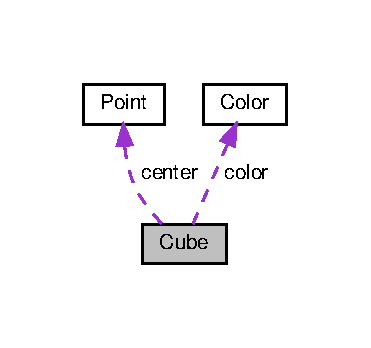
\includegraphics[width=178pt]{struct_cube__coll__graph}
\end{center}
\end{figure}
\subsection*{Data Fields}
\begin{DoxyCompactItemize}
\item 
\hyperlink{g3x__transfo_8h_a89b2b23e407882a535d835574a7912e1}{double} \hyperlink{struct_cube_a2459aedac9f8646ad9566164a9a83f41}{rayon}
\item 
\hyperlink{struct_color}{Color} \hyperlink{struct_cube_aa5f4d1eda21c196bd8401ff73f105073}{color}
\item 
\hyperlink{struct_point}{Point} \hyperlink{struct_cube_a24bb1c337bce91dd3e7a4a4372b11793}{center}
\end{DoxyCompactItemize}


\subsection{Detailed Description}
a cube 

\hyperlink{struct_cube}{Cube} is a type representing a cube by its center and its raduis. Its facets are supposed to be parallel to those of the canonical cube. The reason of this limitation is to facilitate the creation of instances. 

\subsection{Field Documentation}
\mbox{\Hypertarget{struct_cube_a24bb1c337bce91dd3e7a4a4372b11793}\label{struct_cube_a24bb1c337bce91dd3e7a4a4372b11793}} 
\index{Cube@{Cube}!center@{center}}
\index{center@{center}!Cube@{Cube}}
\subsubsection{\texorpdfstring{center}{center}}
{\footnotesize\ttfamily \hyperlink{struct_point}{Point} center}

the center of the cube \mbox{\Hypertarget{struct_cube_aa5f4d1eda21c196bd8401ff73f105073}\label{struct_cube_aa5f4d1eda21c196bd8401ff73f105073}} 
\index{Cube@{Cube}!color@{color}}
\index{color@{color}!Cube@{Cube}}
\subsubsection{\texorpdfstring{color}{color}}
{\footnotesize\ttfamily \hyperlink{struct_color}{Color} color}

the color of the cube \mbox{\Hypertarget{struct_cube_a2459aedac9f8646ad9566164a9a83f41}\label{struct_cube_a2459aedac9f8646ad9566164a9a83f41}} 
\index{Cube@{Cube}!rayon@{rayon}}
\index{rayon@{rayon}!Cube@{Cube}}
\subsubsection{\texorpdfstring{rayon}{rayon}}
{\footnotesize\ttfamily \hyperlink{g3x__transfo_8h_a89b2b23e407882a535d835574a7912e1}{double} rayon}

radius of the cube 

The documentation for this struct was generated from the following file\+:\begin{DoxyCompactItemize}
\item 
include/\hyperlink{_cube_8h}{Cube.\+h}\end{DoxyCompactItemize}

\hypertarget{struct_cylindre}{}\section{Cylindre Struct Reference}
\label{struct_cylindre}\index{Cylindre@{Cylindre}}


a cylinder  




{\ttfamily \#include $<$Cylindre.\+h$>$}



Collaboration diagram for Cylindre\+:\nopagebreak
\begin{figure}[H]
\begin{center}
\leavevmode
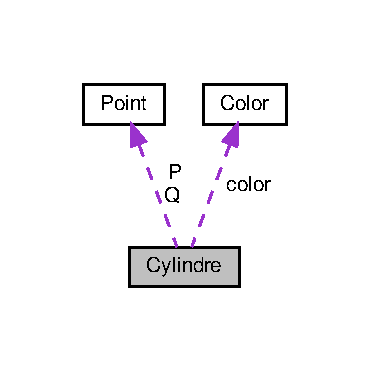
\includegraphics[width=178pt]{struct_cylindre__coll__graph}
\end{center}
\end{figure}
\subsection*{Data Fields}
\begin{DoxyCompactItemize}
\item 
\hyperlink{struct_color}{Color} \hyperlink{struct_cylindre_aa5f4d1eda21c196bd8401ff73f105073}{color}
\item 
\hyperlink{g3x__transfo_8h_a89b2b23e407882a535d835574a7912e1}{double} \hyperlink{struct_cylindre_a2459aedac9f8646ad9566164a9a83f41}{rayon}
\item 
\hyperlink{struct_point}{Point} \hyperlink{struct_cylindre_a8c362b40598e0f5315cbcd092760c0d2}{P}
\item 
\hyperlink{struct_point}{Point} \hyperlink{struct_cylindre_a20c58d187415dcf2911db42e12d5ee05}{Q}
\end{DoxyCompactItemize}


\subsection{Detailed Description}
a cylinder 

a cylinder is defined by two points and the raduis, the axis of the cylinder is the line (PQ) the hight of the cylinder is the distance PQ 

\subsection{Field Documentation}
\mbox{\Hypertarget{struct_cylindre_aa5f4d1eda21c196bd8401ff73f105073}\label{struct_cylindre_aa5f4d1eda21c196bd8401ff73f105073}} 
\index{Cylindre@{Cylindre}!color@{color}}
\index{color@{color}!Cylindre@{Cylindre}}
\subsubsection{\texorpdfstring{color}{color}}
{\footnotesize\ttfamily \hyperlink{struct_color}{Color} color}

the color of the cylinder \mbox{\Hypertarget{struct_cylindre_a8c362b40598e0f5315cbcd092760c0d2}\label{struct_cylindre_a8c362b40598e0f5315cbcd092760c0d2}} 
\index{Cylindre@{Cylindre}!P@{P}}
\index{P@{P}!Cylindre@{Cylindre}}
\subsubsection{\texorpdfstring{P}{P}}
{\footnotesize\ttfamily \hyperlink{struct_point}{Point} P}

the center of the 1st face of the cylinder \mbox{\Hypertarget{struct_cylindre_a20c58d187415dcf2911db42e12d5ee05}\label{struct_cylindre_a20c58d187415dcf2911db42e12d5ee05}} 
\index{Cylindre@{Cylindre}!Q@{Q}}
\index{Q@{Q}!Cylindre@{Cylindre}}
\subsubsection{\texorpdfstring{Q}{Q}}
{\footnotesize\ttfamily \hyperlink{struct_point}{Point} Q}

the center of the 2nd face of the cylinder \mbox{\Hypertarget{struct_cylindre_a2459aedac9f8646ad9566164a9a83f41}\label{struct_cylindre_a2459aedac9f8646ad9566164a9a83f41}} 
\index{Cylindre@{Cylindre}!rayon@{rayon}}
\index{rayon@{rayon}!Cylindre@{Cylindre}}
\subsubsection{\texorpdfstring{rayon}{rayon}}
{\footnotesize\ttfamily \hyperlink{g3x__transfo_8h_a89b2b23e407882a535d835574a7912e1}{double} rayon}

the radius of the cylinder 

The documentation for this struct was generated from the following file\+:\begin{DoxyCompactItemize}
\item 
include/\hyperlink{_cylindre_8h}{Cylindre.\+h}\end{DoxyCompactItemize}

\hypertarget{struct_g3_xadres}{}\section{G3\+Xadres Struct Reference}
\label{struct_g3_xadres}\index{G3\+Xadres@{G3\+Xadres}}
\subsection*{Data Fields}
\begin{DoxyCompactItemize}
\item 
\hyperlink{g3x__transfo_8h_a89b2b23e407882a535d835574a7912e1}{double} $\ast$ \hyperlink{struct_g3_xadres_a318ae30f1efdf8759037f1c91f96a3a6}{r}
\item 
int $\ast$ \hyperlink{struct_g3_xadres_a9384343c8d6a756c1d78cdc73d351b8e}{i}
\end{DoxyCompactItemize}


\subsection{Field Documentation}
\mbox{\Hypertarget{struct_g3_xadres_a9384343c8d6a756c1d78cdc73d351b8e}\label{struct_g3_xadres_a9384343c8d6a756c1d78cdc73d351b8e}} 
\index{G3\+Xadres@{G3\+Xadres}!i@{i}}
\index{i@{i}!G3\+Xadres@{G3\+Xadres}}
\subsubsection{\texorpdfstring{i}{i}}
{\footnotesize\ttfamily int$\ast$ i}

\mbox{\Hypertarget{struct_g3_xadres_a318ae30f1efdf8759037f1c91f96a3a6}\label{struct_g3_xadres_a318ae30f1efdf8759037f1c91f96a3a6}} 
\index{G3\+Xadres@{G3\+Xadres}!r@{r}}
\index{r@{r}!G3\+Xadres@{G3\+Xadres}}
\subsubsection{\texorpdfstring{r}{r}}
{\footnotesize\ttfamily \hyperlink{g3x__transfo_8h_a89b2b23e407882a535d835574a7912e1}{double}$\ast$ r}



The documentation for this struct was generated from the following file\+:\begin{DoxyCompactItemize}
\item 
libg3x/src/\hyperlink{g3x__ctrlprm_8c}{g3x\+\_\+ctrlprm.\+c}\end{DoxyCompactItemize}

\hypertarget{struct_g3_xbut}{}\section{G3\+Xbut Struct Reference}
\label{struct_g3_xbut}\index{G3\+Xbut@{G3\+Xbut}}
\subsection*{Data Fields}
\begin{DoxyCompactItemize}
\item 
int \hyperlink{struct_g3_xbut_a86cf672daa4e0ad11ad10efc894d19c8}{num}
\item 
int \hyperlink{struct_g3_xbut_a6150e0515f7202e2fb518f7206ed97dc}{x}
\item 
int \hyperlink{struct_g3_xbut_a0a2f84ed7838f07779ae24c5a9086d33}{y}
\item 
int \hyperlink{struct_g3_xbut_afed088663f8704004425cdae2120b9b3}{len}
\item 
char \hyperlink{struct_g3_xbut_aa998d085055b9e9634ea1781cc0163c7}{name} \mbox{[}\hyperlink{g3x__switch_8c_a0e40ba0c0da54aafd8c34999455ec4fa}{M\+A\+X\+B\+U\+T\+L\+EN}+1\mbox{]}
\item 
char \hyperlink{struct_g3_xbut_aef383a8ccd6a48889b57cb6ceb7091f6}{info} \mbox{[}128\mbox{]}
\item 
\hyperlink{g3x__types_8h_af6a258d8f3ee5206d682d799316314b1}{bool} \hyperlink{struct_g3_xbut_aaa928c9a62449f7946da1e32f66c70d2}{on}
\end{DoxyCompactItemize}


\subsection{Field Documentation}
\mbox{\Hypertarget{struct_g3_xbut_aef383a8ccd6a48889b57cb6ceb7091f6}\label{struct_g3_xbut_aef383a8ccd6a48889b57cb6ceb7091f6}} 
\index{G3\+Xbut@{G3\+Xbut}!info@{info}}
\index{info@{info}!G3\+Xbut@{G3\+Xbut}}
\subsubsection{\texorpdfstring{info}{info}}
{\footnotesize\ttfamily char info\mbox{[}128\mbox{]}}

\mbox{\Hypertarget{struct_g3_xbut_afed088663f8704004425cdae2120b9b3}\label{struct_g3_xbut_afed088663f8704004425cdae2120b9b3}} 
\index{G3\+Xbut@{G3\+Xbut}!len@{len}}
\index{len@{len}!G3\+Xbut@{G3\+Xbut}}
\subsubsection{\texorpdfstring{len}{len}}
{\footnotesize\ttfamily int len}

\mbox{\Hypertarget{struct_g3_xbut_aa998d085055b9e9634ea1781cc0163c7}\label{struct_g3_xbut_aa998d085055b9e9634ea1781cc0163c7}} 
\index{G3\+Xbut@{G3\+Xbut}!name@{name}}
\index{name@{name}!G3\+Xbut@{G3\+Xbut}}
\subsubsection{\texorpdfstring{name}{name}}
{\footnotesize\ttfamily char name\mbox{[}\hyperlink{g3x__switch_8c_a0e40ba0c0da54aafd8c34999455ec4fa}{M\+A\+X\+B\+U\+T\+L\+EN}+1\mbox{]}}

\mbox{\Hypertarget{struct_g3_xbut_a86cf672daa4e0ad11ad10efc894d19c8}\label{struct_g3_xbut_a86cf672daa4e0ad11ad10efc894d19c8}} 
\index{G3\+Xbut@{G3\+Xbut}!num@{num}}
\index{num@{num}!G3\+Xbut@{G3\+Xbut}}
\subsubsection{\texorpdfstring{num}{num}}
{\footnotesize\ttfamily int num}

\mbox{\Hypertarget{struct_g3_xbut_aaa928c9a62449f7946da1e32f66c70d2}\label{struct_g3_xbut_aaa928c9a62449f7946da1e32f66c70d2}} 
\index{G3\+Xbut@{G3\+Xbut}!on@{on}}
\index{on@{on}!G3\+Xbut@{G3\+Xbut}}
\subsubsection{\texorpdfstring{on}{on}}
{\footnotesize\ttfamily \hyperlink{g3x__types_8h_af6a258d8f3ee5206d682d799316314b1}{bool} on}

\mbox{\Hypertarget{struct_g3_xbut_a6150e0515f7202e2fb518f7206ed97dc}\label{struct_g3_xbut_a6150e0515f7202e2fb518f7206ed97dc}} 
\index{G3\+Xbut@{G3\+Xbut}!x@{x}}
\index{x@{x}!G3\+Xbut@{G3\+Xbut}}
\subsubsection{\texorpdfstring{x}{x}}
{\footnotesize\ttfamily int x}

\mbox{\Hypertarget{struct_g3_xbut_a0a2f84ed7838f07779ae24c5a9086d33}\label{struct_g3_xbut_a0a2f84ed7838f07779ae24c5a9086d33}} 
\index{G3\+Xbut@{G3\+Xbut}!y@{y}}
\index{y@{y}!G3\+Xbut@{G3\+Xbut}}
\subsubsection{\texorpdfstring{y}{y}}
{\footnotesize\ttfamily int y}



The documentation for this struct was generated from the following file\+:\begin{DoxyCompactItemize}
\item 
libg3x/src/\hyperlink{g3x__button_8c}{g3x\+\_\+button.\+c}\end{DoxyCompactItemize}

\hypertarget{struct_g3_xcamera}{}\section{G3\+Xcamera Struct Reference}
\label{struct_g3_xcamera}\index{G3\+Xcamera@{G3\+Xcamera}}


{\ttfamily \#include $<$g3x\+\_\+types.\+h$>$}

\subsection*{Data Fields}
\begin{DoxyCompactItemize}
\item 
\hyperlink{g3x__types_8h_a656d1bc95bdef5a54decde84cfe9f60a}{G3\+Xpoint} $\ast$ \hyperlink{struct_g3_xcamera_a89b7ccb5e6816ed54f59a9617a904f87}{pos}
\item 
\hyperlink{g3x__types_8h_a656d1bc95bdef5a54decde84cfe9f60a}{G3\+Xpoint} $\ast$ \hyperlink{struct_g3_xcamera_a9e81d1c93b5922975305fc19baee7b2e}{tar}
\item 
\hyperlink{g3x__types_8h_a6181ad7c7bac1d7942ab3944bae2b8a1}{G3\+Xvector} \hyperlink{struct_g3_xcamera_adc4802615d8f0d628d8b2986f08bbce8}{upv}
\item 
\hyperlink{g3x__transfo_8h_a89b2b23e407882a535d835574a7912e1}{double} \hyperlink{struct_g3_xcamera_aca81c35c21e3a5f7f3a8d24504e76664}{theta}
\item 
\hyperlink{g3x__transfo_8h_a89b2b23e407882a535d835574a7912e1}{double} \hyperlink{struct_g3_xcamera_adae8d8a6ff28515e505bb1c07f2b33c8}{phi}
\item 
\hyperlink{g3x__transfo_8h_a89b2b23e407882a535d835574a7912e1}{double} \hyperlink{struct_g3_xcamera_accf93555161c9eedf006462a228af523}{dist}
\item 
\hyperlink{g3x__transfo_8h_a89b2b23e407882a535d835574a7912e1}{double} \hyperlink{struct_g3_xcamera_a3b79efd873843125dabba312ddde65a3}{near}
\item 
\hyperlink{g3x__transfo_8h_a89b2b23e407882a535d835574a7912e1}{double} \hyperlink{struct_g3_xcamera_add1a608db25e8e3befb6775a16867611}{far}
\item 
\hyperlink{g3x__transfo_8h_a89b2b23e407882a535d835574a7912e1}{double} \hyperlink{struct_g3_xcamera_a4ef60f0d779b1928bb150cab69726bab}{open}
\end{DoxyCompactItemize}


\subsection{Field Documentation}
\mbox{\Hypertarget{struct_g3_xcamera_accf93555161c9eedf006462a228af523}\label{struct_g3_xcamera_accf93555161c9eedf006462a228af523}} 
\index{G3\+Xcamera@{G3\+Xcamera}!dist@{dist}}
\index{dist@{dist}!G3\+Xcamera@{G3\+Xcamera}}
\subsubsection{\texorpdfstring{dist}{dist}}
{\footnotesize\ttfamily \hyperlink{g3x__transfo_8h_a89b2b23e407882a535d835574a7912e1}{double} dist}

\mbox{\Hypertarget{struct_g3_xcamera_add1a608db25e8e3befb6775a16867611}\label{struct_g3_xcamera_add1a608db25e8e3befb6775a16867611}} 
\index{G3\+Xcamera@{G3\+Xcamera}!far@{far}}
\index{far@{far}!G3\+Xcamera@{G3\+Xcamera}}
\subsubsection{\texorpdfstring{far}{far}}
{\footnotesize\ttfamily \hyperlink{g3x__transfo_8h_a89b2b23e407882a535d835574a7912e1}{double} far}

\mbox{\Hypertarget{struct_g3_xcamera_a3b79efd873843125dabba312ddde65a3}\label{struct_g3_xcamera_a3b79efd873843125dabba312ddde65a3}} 
\index{G3\+Xcamera@{G3\+Xcamera}!near@{near}}
\index{near@{near}!G3\+Xcamera@{G3\+Xcamera}}
\subsubsection{\texorpdfstring{near}{near}}
{\footnotesize\ttfamily \hyperlink{g3x__transfo_8h_a89b2b23e407882a535d835574a7912e1}{double} near}

\mbox{\Hypertarget{struct_g3_xcamera_a4ef60f0d779b1928bb150cab69726bab}\label{struct_g3_xcamera_a4ef60f0d779b1928bb150cab69726bab}} 
\index{G3\+Xcamera@{G3\+Xcamera}!open@{open}}
\index{open@{open}!G3\+Xcamera@{G3\+Xcamera}}
\subsubsection{\texorpdfstring{open}{open}}
{\footnotesize\ttfamily \hyperlink{g3x__transfo_8h_a89b2b23e407882a535d835574a7912e1}{double} open}

\mbox{\Hypertarget{struct_g3_xcamera_adae8d8a6ff28515e505bb1c07f2b33c8}\label{struct_g3_xcamera_adae8d8a6ff28515e505bb1c07f2b33c8}} 
\index{G3\+Xcamera@{G3\+Xcamera}!phi@{phi}}
\index{phi@{phi}!G3\+Xcamera@{G3\+Xcamera}}
\subsubsection{\texorpdfstring{phi}{phi}}
{\footnotesize\ttfamily \hyperlink{g3x__transfo_8h_a89b2b23e407882a535d835574a7912e1}{double} phi}

\mbox{\Hypertarget{struct_g3_xcamera_a89b7ccb5e6816ed54f59a9617a904f87}\label{struct_g3_xcamera_a89b7ccb5e6816ed54f59a9617a904f87}} 
\index{G3\+Xcamera@{G3\+Xcamera}!pos@{pos}}
\index{pos@{pos}!G3\+Xcamera@{G3\+Xcamera}}
\subsubsection{\texorpdfstring{pos}{pos}}
{\footnotesize\ttfamily \hyperlink{g3x__types_8h_a656d1bc95bdef5a54decde84cfe9f60a}{G3\+Xpoint}$\ast$ pos}

\mbox{\Hypertarget{struct_g3_xcamera_a9e81d1c93b5922975305fc19baee7b2e}\label{struct_g3_xcamera_a9e81d1c93b5922975305fc19baee7b2e}} 
\index{G3\+Xcamera@{G3\+Xcamera}!tar@{tar}}
\index{tar@{tar}!G3\+Xcamera@{G3\+Xcamera}}
\subsubsection{\texorpdfstring{tar}{tar}}
{\footnotesize\ttfamily \hyperlink{g3x__types_8h_a656d1bc95bdef5a54decde84cfe9f60a}{G3\+Xpoint}$\ast$ tar}

\mbox{\Hypertarget{struct_g3_xcamera_aca81c35c21e3a5f7f3a8d24504e76664}\label{struct_g3_xcamera_aca81c35c21e3a5f7f3a8d24504e76664}} 
\index{G3\+Xcamera@{G3\+Xcamera}!theta@{theta}}
\index{theta@{theta}!G3\+Xcamera@{G3\+Xcamera}}
\subsubsection{\texorpdfstring{theta}{theta}}
{\footnotesize\ttfamily \hyperlink{g3x__transfo_8h_a89b2b23e407882a535d835574a7912e1}{double} theta}

\mbox{\Hypertarget{struct_g3_xcamera_adc4802615d8f0d628d8b2986f08bbce8}\label{struct_g3_xcamera_adc4802615d8f0d628d8b2986f08bbce8}} 
\index{G3\+Xcamera@{G3\+Xcamera}!upv@{upv}}
\index{upv@{upv}!G3\+Xcamera@{G3\+Xcamera}}
\subsubsection{\texorpdfstring{upv}{upv}}
{\footnotesize\ttfamily \hyperlink{g3x__types_8h_a6181ad7c7bac1d7942ab3944bae2b8a1}{G3\+Xvector} upv}



The documentation for this struct was generated from the following file\+:\begin{DoxyCompactItemize}
\item 
libg3x/include/\hyperlink{g3x__types_8h}{g3x\+\_\+types.\+h}\end{DoxyCompactItemize}

\hypertarget{struct_g3_xclock}{}\section{G3\+Xclock Struct Reference}
\label{struct_g3_xclock}\index{G3\+Xclock@{G3\+Xclock}}


{\ttfamily \#include $<$g3x\+\_\+types.\+h$>$}

\subsection*{Data Fields}
\begin{DoxyCompactItemize}
\item 
\hyperlink{g3x__types_8h_a91ad9478d81a7aaf2593e8d9c3d06a14}{uint} \hyperlink{struct_g3_xclock_a4d1ee55639956a3794ee81419b4f5f7a}{hh}
\item 
\hyperlink{g3x__types_8h_a91ad9478d81a7aaf2593e8d9c3d06a14}{uint} \hyperlink{struct_g3_xclock_ab2620c15993ec02d8ae073176ff74f8b}{mm}
\item 
\hyperlink{g3x__types_8h_a91ad9478d81a7aaf2593e8d9c3d06a14}{uint} \hyperlink{struct_g3_xclock_a3f8b4c08b00b9b0cc37cbb88d9f759ca}{ss}
\item 
\hyperlink{g3x__types_8h_a91ad9478d81a7aaf2593e8d9c3d06a14}{uint} \hyperlink{struct_g3_xclock_a101cd9996b0099b01cb6a1594bad1058}{ds}
\item 
\hyperlink{g3x__types_8h_a91ad9478d81a7aaf2593e8d9c3d06a14}{uint} \hyperlink{struct_g3_xclock_a21ff1dca4ee9146feae362cb81bdb73b}{cs}
\item 
\hyperlink{g3x__types_8h_a91ad9478d81a7aaf2593e8d9c3d06a14}{uint} \hyperlink{struct_g3_xclock_a0bcb3d72edad5c1ecf1c931e37128d15}{ms}
\end{DoxyCompactItemize}


\subsection{Field Documentation}
\mbox{\Hypertarget{struct_g3_xclock_a21ff1dca4ee9146feae362cb81bdb73b}\label{struct_g3_xclock_a21ff1dca4ee9146feae362cb81bdb73b}} 
\index{G3\+Xclock@{G3\+Xclock}!cs@{cs}}
\index{cs@{cs}!G3\+Xclock@{G3\+Xclock}}
\subsubsection{\texorpdfstring{cs}{cs}}
{\footnotesize\ttfamily \hyperlink{g3x__types_8h_a91ad9478d81a7aaf2593e8d9c3d06a14}{uint} cs}

\mbox{\Hypertarget{struct_g3_xclock_a101cd9996b0099b01cb6a1594bad1058}\label{struct_g3_xclock_a101cd9996b0099b01cb6a1594bad1058}} 
\index{G3\+Xclock@{G3\+Xclock}!ds@{ds}}
\index{ds@{ds}!G3\+Xclock@{G3\+Xclock}}
\subsubsection{\texorpdfstring{ds}{ds}}
{\footnotesize\ttfamily \hyperlink{g3x__types_8h_a91ad9478d81a7aaf2593e8d9c3d06a14}{uint} ds}

\mbox{\Hypertarget{struct_g3_xclock_a4d1ee55639956a3794ee81419b4f5f7a}\label{struct_g3_xclock_a4d1ee55639956a3794ee81419b4f5f7a}} 
\index{G3\+Xclock@{G3\+Xclock}!hh@{hh}}
\index{hh@{hh}!G3\+Xclock@{G3\+Xclock}}
\subsubsection{\texorpdfstring{hh}{hh}}
{\footnotesize\ttfamily \hyperlink{g3x__types_8h_a91ad9478d81a7aaf2593e8d9c3d06a14}{uint} hh}

\mbox{\Hypertarget{struct_g3_xclock_ab2620c15993ec02d8ae073176ff74f8b}\label{struct_g3_xclock_ab2620c15993ec02d8ae073176ff74f8b}} 
\index{G3\+Xclock@{G3\+Xclock}!mm@{mm}}
\index{mm@{mm}!G3\+Xclock@{G3\+Xclock}}
\subsubsection{\texorpdfstring{mm}{mm}}
{\footnotesize\ttfamily \hyperlink{g3x__types_8h_a91ad9478d81a7aaf2593e8d9c3d06a14}{uint} mm}

\mbox{\Hypertarget{struct_g3_xclock_a0bcb3d72edad5c1ecf1c931e37128d15}\label{struct_g3_xclock_a0bcb3d72edad5c1ecf1c931e37128d15}} 
\index{G3\+Xclock@{G3\+Xclock}!ms@{ms}}
\index{ms@{ms}!G3\+Xclock@{G3\+Xclock}}
\subsubsection{\texorpdfstring{ms}{ms}}
{\footnotesize\ttfamily \hyperlink{g3x__types_8h_a91ad9478d81a7aaf2593e8d9c3d06a14}{uint} ms}

\mbox{\Hypertarget{struct_g3_xclock_a3f8b4c08b00b9b0cc37cbb88d9f759ca}\label{struct_g3_xclock_a3f8b4c08b00b9b0cc37cbb88d9f759ca}} 
\index{G3\+Xclock@{G3\+Xclock}!ss@{ss}}
\index{ss@{ss}!G3\+Xclock@{G3\+Xclock}}
\subsubsection{\texorpdfstring{ss}{ss}}
{\footnotesize\ttfamily \hyperlink{g3x__types_8h_a91ad9478d81a7aaf2593e8d9c3d06a14}{uint} ss}



The documentation for this struct was generated from the following file\+:\begin{DoxyCompactItemize}
\item 
libg3x/include/\hyperlink{g3x__types_8h}{g3x\+\_\+types.\+h}\end{DoxyCompactItemize}

\hypertarget{struct_g3_ximgnames}{}\section{G3\+Ximgnames Struct Reference}
\label{struct_g3_ximgnames}\index{G3\+Ximgnames@{G3\+Ximgnames}}


Collaboration diagram for G3\+Ximgnames\+:\nopagebreak
\begin{figure}[H]
\begin{center}
\leavevmode
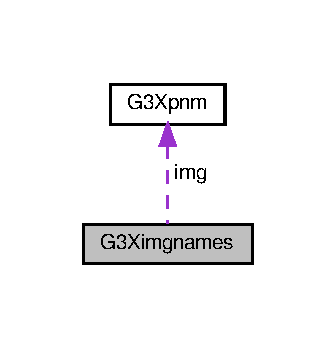
\includegraphics[width=161pt]{struct_g3_ximgnames__coll__graph}
\end{center}
\end{figure}
\subsection*{Data Fields}
\begin{DoxyCompactItemize}
\item 
\hyperlink{struct_g3_xpnm}{G3\+Xpnm} $\ast$ \hyperlink{struct_g3_ximgnames_a3ea0190663b3990ebc8f0be8730998c3}{img}
\item 
char \hyperlink{struct_g3_ximgnames_ac2cd9523d5ab409e403a59e0e21f114a}{name} \mbox{[}\hyperlink{g3x__pnm_8c_a56739a38cf3fb0c5d7d842fe94f96f86}{M\+A\+X\+N\+A\+M\+E\+L\+EN}+1\mbox{]}
\end{DoxyCompactItemize}


\subsection{Field Documentation}
\mbox{\Hypertarget{struct_g3_ximgnames_a3ea0190663b3990ebc8f0be8730998c3}\label{struct_g3_ximgnames_a3ea0190663b3990ebc8f0be8730998c3}} 
\index{G3\+Ximgnames@{G3\+Ximgnames}!img@{img}}
\index{img@{img}!G3\+Ximgnames@{G3\+Ximgnames}}
\subsubsection{\texorpdfstring{img}{img}}
{\footnotesize\ttfamily \hyperlink{struct_g3_xpnm}{G3\+Xpnm}$\ast$ img}

\mbox{\Hypertarget{struct_g3_ximgnames_ac2cd9523d5ab409e403a59e0e21f114a}\label{struct_g3_ximgnames_ac2cd9523d5ab409e403a59e0e21f114a}} 
\index{G3\+Ximgnames@{G3\+Ximgnames}!name@{name}}
\index{name@{name}!G3\+Ximgnames@{G3\+Ximgnames}}
\subsubsection{\texorpdfstring{name}{name}}
{\footnotesize\ttfamily char name\mbox{[}\hyperlink{g3x__pnm_8c_a56739a38cf3fb0c5d7d842fe94f96f86}{M\+A\+X\+N\+A\+M\+E\+L\+EN}+1\mbox{]}}



The documentation for this struct was generated from the following file\+:\begin{DoxyCompactItemize}
\item 
libg3x/src/\hyperlink{g3x__pnm_8c}{g3x\+\_\+pnm.\+c}\end{DoxyCompactItemize}

\hypertarget{struct_g3_xkey}{}\section{G3\+Xkey Struct Reference}
\label{struct_g3_xkey}\index{G3\+Xkey@{G3\+Xkey}}
\subsection*{Data Fields}
\begin{DoxyCompactItemize}
\item 
void($\ast$ \hyperlink{struct_g3_xkey_ab9b939162161b10361618af747095d06}{action} )()
\item 
char \hyperlink{struct_g3_xkey_acad36f7a1211e9e9da68e181667d9c3f}{key}
\item 
char \hyperlink{struct_g3_xkey_a27acbfc0545ba6b07ee04d1be61713c8}{info} \mbox{[}64\mbox{]}
\end{DoxyCompactItemize}


\subsection{Field Documentation}
\mbox{\Hypertarget{struct_g3_xkey_ab9b939162161b10361618af747095d06}\label{struct_g3_xkey_ab9b939162161b10361618af747095d06}} 
\index{G3\+Xkey@{G3\+Xkey}!action@{action}}
\index{action@{action}!G3\+Xkey@{G3\+Xkey}}
\subsubsection{\texorpdfstring{action}{action}}
{\footnotesize\ttfamily void($\ast$ action) ()}

\mbox{\Hypertarget{struct_g3_xkey_a27acbfc0545ba6b07ee04d1be61713c8}\label{struct_g3_xkey_a27acbfc0545ba6b07ee04d1be61713c8}} 
\index{G3\+Xkey@{G3\+Xkey}!info@{info}}
\index{info@{info}!G3\+Xkey@{G3\+Xkey}}
\subsubsection{\texorpdfstring{info}{info}}
{\footnotesize\ttfamily char info\mbox{[}64\mbox{]}}

\mbox{\Hypertarget{struct_g3_xkey_acad36f7a1211e9e9da68e181667d9c3f}\label{struct_g3_xkey_acad36f7a1211e9e9da68e181667d9c3f}} 
\index{G3\+Xkey@{G3\+Xkey}!key@{key}}
\index{key@{key}!G3\+Xkey@{G3\+Xkey}}
\subsubsection{\texorpdfstring{key}{key}}
{\footnotesize\ttfamily char key}



The documentation for this struct was generated from the following file\+:\begin{DoxyCompactItemize}
\item 
libg3x/src/\hyperlink{g3x__keys_8c}{g3x\+\_\+keys.\+c}\end{DoxyCompactItemize}

\hypertarget{struct_g3_xlight}{}\section{G3\+Xlight Struct Reference}
\label{struct_g3_xlight}\index{G3\+Xlight@{G3\+Xlight}}


{\ttfamily \#include $<$g3x\+\_\+types.\+h$>$}

\subsection*{Data Fields}
\begin{DoxyCompactItemize}
\item 
\hyperlink{g3x__types_8h_a656d1bc95bdef5a54decde84cfe9f60a}{G3\+Xpoint} \hyperlink{struct_g3_xlight_a853e10d13368ee8dc352141cce54f7f8}{pos}
\item 
\hyperlink{g3x__transfo_8h_a89b2b23e407882a535d835574a7912e1}{double} \hyperlink{struct_g3_xlight_aca81c35c21e3a5f7f3a8d24504e76664}{theta}
\item 
\hyperlink{g3x__transfo_8h_a89b2b23e407882a535d835574a7912e1}{double} \hyperlink{struct_g3_xlight_adae8d8a6ff28515e505bb1c07f2b33c8}{phi}
\item 
\hyperlink{g3x__transfo_8h_a89b2b23e407882a535d835574a7912e1}{double} \hyperlink{struct_g3_xlight_accf93555161c9eedf006462a228af523}{dist}
\item 
\hyperlink{g3x__types_8h_afc484f732c62f1a0417034e535352e30}{G3\+Xcolor} \hyperlink{struct_g3_xlight_a2f38453a2432f73c432d6d6c71cf630d}{ambi}
\item 
\hyperlink{g3x__types_8h_afc484f732c62f1a0417034e535352e30}{G3\+Xcolor} \hyperlink{struct_g3_xlight_ab37a07844bff7802809eb22db0fb0b16}{diff}
\item 
\hyperlink{g3x__types_8h_afc484f732c62f1a0417034e535352e30}{G3\+Xcolor} \hyperlink{struct_g3_xlight_a937aebfb58ac178ae9636be149315f36}{spec}
\item 
\hyperlink{g3x__transfo_8h_a89b2b23e407882a535d835574a7912e1}{double} \hyperlink{struct_g3_xlight_a229d11aff11a7482259d1296b9b70b8a}{dx}
\item 
\hyperlink{g3x__transfo_8h_a89b2b23e407882a535d835574a7912e1}{double} \hyperlink{struct_g3_xlight_a9deb6f886b19d50e714d890c3c268efc}{dy}
\item 
\hyperlink{g3x__transfo_8h_a89b2b23e407882a535d835574a7912e1}{double} \hyperlink{struct_g3_xlight_a5a198de8c3f38514f4e55231aa69cd10}{dz}
\end{DoxyCompactItemize}


\subsection{Field Documentation}
\mbox{\Hypertarget{struct_g3_xlight_a2f38453a2432f73c432d6d6c71cf630d}\label{struct_g3_xlight_a2f38453a2432f73c432d6d6c71cf630d}} 
\index{G3\+Xlight@{G3\+Xlight}!ambi@{ambi}}
\index{ambi@{ambi}!G3\+Xlight@{G3\+Xlight}}
\subsubsection{\texorpdfstring{ambi}{ambi}}
{\footnotesize\ttfamily \hyperlink{g3x__types_8h_afc484f732c62f1a0417034e535352e30}{G3\+Xcolor} ambi}

\mbox{\Hypertarget{struct_g3_xlight_ab37a07844bff7802809eb22db0fb0b16}\label{struct_g3_xlight_ab37a07844bff7802809eb22db0fb0b16}} 
\index{G3\+Xlight@{G3\+Xlight}!diff@{diff}}
\index{diff@{diff}!G3\+Xlight@{G3\+Xlight}}
\subsubsection{\texorpdfstring{diff}{diff}}
{\footnotesize\ttfamily \hyperlink{g3x__types_8h_afc484f732c62f1a0417034e535352e30}{G3\+Xcolor} diff}

\mbox{\Hypertarget{struct_g3_xlight_accf93555161c9eedf006462a228af523}\label{struct_g3_xlight_accf93555161c9eedf006462a228af523}} 
\index{G3\+Xlight@{G3\+Xlight}!dist@{dist}}
\index{dist@{dist}!G3\+Xlight@{G3\+Xlight}}
\subsubsection{\texorpdfstring{dist}{dist}}
{\footnotesize\ttfamily \hyperlink{g3x__transfo_8h_a89b2b23e407882a535d835574a7912e1}{double} dist}

\mbox{\Hypertarget{struct_g3_xlight_a229d11aff11a7482259d1296b9b70b8a}\label{struct_g3_xlight_a229d11aff11a7482259d1296b9b70b8a}} 
\index{G3\+Xlight@{G3\+Xlight}!dx@{dx}}
\index{dx@{dx}!G3\+Xlight@{G3\+Xlight}}
\subsubsection{\texorpdfstring{dx}{dx}}
{\footnotesize\ttfamily \hyperlink{g3x__transfo_8h_a89b2b23e407882a535d835574a7912e1}{double} dx}

\mbox{\Hypertarget{struct_g3_xlight_a9deb6f886b19d50e714d890c3c268efc}\label{struct_g3_xlight_a9deb6f886b19d50e714d890c3c268efc}} 
\index{G3\+Xlight@{G3\+Xlight}!dy@{dy}}
\index{dy@{dy}!G3\+Xlight@{G3\+Xlight}}
\subsubsection{\texorpdfstring{dy}{dy}}
{\footnotesize\ttfamily \hyperlink{g3x__transfo_8h_a89b2b23e407882a535d835574a7912e1}{double} dy}

\mbox{\Hypertarget{struct_g3_xlight_a5a198de8c3f38514f4e55231aa69cd10}\label{struct_g3_xlight_a5a198de8c3f38514f4e55231aa69cd10}} 
\index{G3\+Xlight@{G3\+Xlight}!dz@{dz}}
\index{dz@{dz}!G3\+Xlight@{G3\+Xlight}}
\subsubsection{\texorpdfstring{dz}{dz}}
{\footnotesize\ttfamily \hyperlink{g3x__transfo_8h_a89b2b23e407882a535d835574a7912e1}{double} dz}

\mbox{\Hypertarget{struct_g3_xlight_adae8d8a6ff28515e505bb1c07f2b33c8}\label{struct_g3_xlight_adae8d8a6ff28515e505bb1c07f2b33c8}} 
\index{G3\+Xlight@{G3\+Xlight}!phi@{phi}}
\index{phi@{phi}!G3\+Xlight@{G3\+Xlight}}
\subsubsection{\texorpdfstring{phi}{phi}}
{\footnotesize\ttfamily \hyperlink{g3x__transfo_8h_a89b2b23e407882a535d835574a7912e1}{double} phi}

\mbox{\Hypertarget{struct_g3_xlight_a853e10d13368ee8dc352141cce54f7f8}\label{struct_g3_xlight_a853e10d13368ee8dc352141cce54f7f8}} 
\index{G3\+Xlight@{G3\+Xlight}!pos@{pos}}
\index{pos@{pos}!G3\+Xlight@{G3\+Xlight}}
\subsubsection{\texorpdfstring{pos}{pos}}
{\footnotesize\ttfamily \hyperlink{g3x__types_8h_a656d1bc95bdef5a54decde84cfe9f60a}{G3\+Xpoint} pos}

\mbox{\Hypertarget{struct_g3_xlight_a937aebfb58ac178ae9636be149315f36}\label{struct_g3_xlight_a937aebfb58ac178ae9636be149315f36}} 
\index{G3\+Xlight@{G3\+Xlight}!spec@{spec}}
\index{spec@{spec}!G3\+Xlight@{G3\+Xlight}}
\subsubsection{\texorpdfstring{spec}{spec}}
{\footnotesize\ttfamily \hyperlink{g3x__types_8h_afc484f732c62f1a0417034e535352e30}{G3\+Xcolor} spec}

\mbox{\Hypertarget{struct_g3_xlight_aca81c35c21e3a5f7f3a8d24504e76664}\label{struct_g3_xlight_aca81c35c21e3a5f7f3a8d24504e76664}} 
\index{G3\+Xlight@{G3\+Xlight}!theta@{theta}}
\index{theta@{theta}!G3\+Xlight@{G3\+Xlight}}
\subsubsection{\texorpdfstring{theta}{theta}}
{\footnotesize\ttfamily \hyperlink{g3x__transfo_8h_a89b2b23e407882a535d835574a7912e1}{double} theta}



The documentation for this struct was generated from the following file\+:\begin{DoxyCompactItemize}
\item 
libg3x/include/\hyperlink{g3x__types_8h}{g3x\+\_\+types.\+h}\end{DoxyCompactItemize}

\hypertarget{struct_g3_xparam}{}\section{G3\+Xparam Struct Reference}
\label{struct_g3_xparam}\index{G3\+Xparam@{G3\+Xparam}}
\subsection*{Data Fields}
\begin{DoxyCompactItemize}
\item 
\hyperlink{g3x__transfo_8h_a89b2b23e407882a535d835574a7912e1}{double} \hyperlink{struct_g3_xparam_a880a49112fedae68e714341a9a082fb6}{r}
\item 
int \hyperlink{struct_g3_xparam_acb559820d9ca11295b4500f179ef6392}{i}
\end{DoxyCompactItemize}


\subsection{Field Documentation}
\mbox{\Hypertarget{struct_g3_xparam_acb559820d9ca11295b4500f179ef6392}\label{struct_g3_xparam_acb559820d9ca11295b4500f179ef6392}} 
\index{G3\+Xparam@{G3\+Xparam}!i@{i}}
\index{i@{i}!G3\+Xparam@{G3\+Xparam}}
\subsubsection{\texorpdfstring{i}{i}}
{\footnotesize\ttfamily int i}

\mbox{\Hypertarget{struct_g3_xparam_a880a49112fedae68e714341a9a082fb6}\label{struct_g3_xparam_a880a49112fedae68e714341a9a082fb6}} 
\index{G3\+Xparam@{G3\+Xparam}!r@{r}}
\index{r@{r}!G3\+Xparam@{G3\+Xparam}}
\subsubsection{\texorpdfstring{r}{r}}
{\footnotesize\ttfamily \hyperlink{g3x__transfo_8h_a89b2b23e407882a535d835574a7912e1}{double} r}



The documentation for this struct was generated from the following file\+:\begin{DoxyCompactItemize}
\item 
libg3x/src/\hyperlink{g3x__ctrlprm_8c}{g3x\+\_\+ctrlprm.\+c}\end{DoxyCompactItemize}

\hypertarget{struct_g3_xpnm}{}\section{G3\+Xpnm Struct Reference}
\label{struct_g3_xpnm}\index{G3\+Xpnm@{G3\+Xpnm}}


{\ttfamily \#include $<$g3x\+\_\+pnm.\+h$>$}

\subsection*{Data Fields}
\begin{DoxyCompactItemize}
\item 
char \hyperlink{struct_g3_xpnm_a000e34997df38c2005a83d63e67d9282}{mode}
\item 
int \hyperlink{struct_g3_xpnm_a2474a5474cbff19523a51eb1de01cda4}{width}
\item 
int \hyperlink{struct_g3_xpnm_ad12fc34ce789bce6c8a05d8a17138534}{height}
\item 
int \hyperlink{struct_g3_xpnm_af5e6403cb6864751421a5e7249e4cc62}{layer}
\item 
int \hyperlink{struct_g3_xpnm_acb5ba97551079e0b072c62c21d784ac5}{depth}
\item 
\hyperlink{g3x__types_8h_a65f85814a8290f9797005d3b28e7e5fc}{uchar} $\ast$ \hyperlink{struct_g3_xpnm_a000e8e2f53a1c0edd509f9a125c24d09}{map}
\item 
\hyperlink{g3x__types_8h_a65f85814a8290f9797005d3b28e7e5fc}{uchar} $\ast$ \hyperlink{struct_g3_xpnm_a213099dd72c580e63fc2c3113b8a1368}{end}
\end{DoxyCompactItemize}


\subsection{Field Documentation}
\mbox{\Hypertarget{struct_g3_xpnm_acb5ba97551079e0b072c62c21d784ac5}\label{struct_g3_xpnm_acb5ba97551079e0b072c62c21d784ac5}} 
\index{G3\+Xpnm@{G3\+Xpnm}!depth@{depth}}
\index{depth@{depth}!G3\+Xpnm@{G3\+Xpnm}}
\subsubsection{\texorpdfstring{depth}{depth}}
{\footnotesize\ttfamily int depth}

\mbox{\Hypertarget{struct_g3_xpnm_a213099dd72c580e63fc2c3113b8a1368}\label{struct_g3_xpnm_a213099dd72c580e63fc2c3113b8a1368}} 
\index{G3\+Xpnm@{G3\+Xpnm}!end@{end}}
\index{end@{end}!G3\+Xpnm@{G3\+Xpnm}}
\subsubsection{\texorpdfstring{end}{end}}
{\footnotesize\ttfamily \hyperlink{g3x__types_8h_a65f85814a8290f9797005d3b28e7e5fc}{uchar} $\ast$ end}

\mbox{\Hypertarget{struct_g3_xpnm_ad12fc34ce789bce6c8a05d8a17138534}\label{struct_g3_xpnm_ad12fc34ce789bce6c8a05d8a17138534}} 
\index{G3\+Xpnm@{G3\+Xpnm}!height@{height}}
\index{height@{height}!G3\+Xpnm@{G3\+Xpnm}}
\subsubsection{\texorpdfstring{height}{height}}
{\footnotesize\ttfamily int height}

\mbox{\Hypertarget{struct_g3_xpnm_af5e6403cb6864751421a5e7249e4cc62}\label{struct_g3_xpnm_af5e6403cb6864751421a5e7249e4cc62}} 
\index{G3\+Xpnm@{G3\+Xpnm}!layer@{layer}}
\index{layer@{layer}!G3\+Xpnm@{G3\+Xpnm}}
\subsubsection{\texorpdfstring{layer}{layer}}
{\footnotesize\ttfamily int layer}

\mbox{\Hypertarget{struct_g3_xpnm_a000e8e2f53a1c0edd509f9a125c24d09}\label{struct_g3_xpnm_a000e8e2f53a1c0edd509f9a125c24d09}} 
\index{G3\+Xpnm@{G3\+Xpnm}!map@{map}}
\index{map@{map}!G3\+Xpnm@{G3\+Xpnm}}
\subsubsection{\texorpdfstring{map}{map}}
{\footnotesize\ttfamily \hyperlink{g3x__types_8h_a65f85814a8290f9797005d3b28e7e5fc}{uchar}$\ast$ map}

\mbox{\Hypertarget{struct_g3_xpnm_a000e34997df38c2005a83d63e67d9282}\label{struct_g3_xpnm_a000e34997df38c2005a83d63e67d9282}} 
\index{G3\+Xpnm@{G3\+Xpnm}!mode@{mode}}
\index{mode@{mode}!G3\+Xpnm@{G3\+Xpnm}}
\subsubsection{\texorpdfstring{mode}{mode}}
{\footnotesize\ttfamily char mode}

\mbox{\Hypertarget{struct_g3_xpnm_a2474a5474cbff19523a51eb1de01cda4}\label{struct_g3_xpnm_a2474a5474cbff19523a51eb1de01cda4}} 
\index{G3\+Xpnm@{G3\+Xpnm}!width@{width}}
\index{width@{width}!G3\+Xpnm@{G3\+Xpnm}}
\subsubsection{\texorpdfstring{width}{width}}
{\footnotesize\ttfamily int width}



The documentation for this struct was generated from the following file\+:\begin{DoxyCompactItemize}
\item 
libg3x/include/\hyperlink{g3x__pnm_8h}{g3x\+\_\+pnm.\+h}\end{DoxyCompactItemize}

\hypertarget{struct_g3_xpopup}{}\section{G3\+Xpopup Struct Reference}
\label{struct_g3_xpopup}\index{G3\+Xpopup@{G3\+Xpopup}}
\subsection*{Data Fields}
\begin{DoxyCompactItemize}
\item 
int \hyperlink{struct_g3_xpopup_a86cf672daa4e0ad11ad10efc894d19c8}{num}
\item 
int \hyperlink{struct_g3_xpopup_a6150e0515f7202e2fb518f7206ed97dc}{x}
\item 
int \hyperlink{struct_g3_xpopup_a0a2f84ed7838f07779ae24c5a9086d33}{y}
\item 
int \hyperlink{struct_g3_xpopup_afed088663f8704004425cdae2120b9b3}{len}
\item 
char \hyperlink{struct_g3_xpopup_aa998d085055b9e9634ea1781cc0163c7}{name} \mbox{[}\hyperlink{g3x__switch_8c_a0e40ba0c0da54aafd8c34999455ec4fa}{M\+A\+X\+B\+U\+T\+L\+EN}+1\mbox{]}
\item 
char \hyperlink{struct_g3_xpopup_aef383a8ccd6a48889b57cb6ceb7091f6}{info} \mbox{[}128\mbox{]}
\item 
void($\ast$ \hyperlink{struct_g3_xpopup_a40c8103d8ace16fc3e34e828fc8bca0b}{action} )(void)
\item 
\hyperlink{g3x__types_8h_af6a258d8f3ee5206d682d799316314b1}{bool} \hyperlink{struct_g3_xpopup_aaa928c9a62449f7946da1e32f66c70d2}{on}
\end{DoxyCompactItemize}


\subsection{Field Documentation}
\mbox{\Hypertarget{struct_g3_xpopup_a40c8103d8ace16fc3e34e828fc8bca0b}\label{struct_g3_xpopup_a40c8103d8ace16fc3e34e828fc8bca0b}} 
\index{G3\+Xpopup@{G3\+Xpopup}!action@{action}}
\index{action@{action}!G3\+Xpopup@{G3\+Xpopup}}
\subsubsection{\texorpdfstring{action}{action}}
{\footnotesize\ttfamily void($\ast$ action) (void)}

\mbox{\Hypertarget{struct_g3_xpopup_aef383a8ccd6a48889b57cb6ceb7091f6}\label{struct_g3_xpopup_aef383a8ccd6a48889b57cb6ceb7091f6}} 
\index{G3\+Xpopup@{G3\+Xpopup}!info@{info}}
\index{info@{info}!G3\+Xpopup@{G3\+Xpopup}}
\subsubsection{\texorpdfstring{info}{info}}
{\footnotesize\ttfamily char info\mbox{[}128\mbox{]}}

\mbox{\Hypertarget{struct_g3_xpopup_afed088663f8704004425cdae2120b9b3}\label{struct_g3_xpopup_afed088663f8704004425cdae2120b9b3}} 
\index{G3\+Xpopup@{G3\+Xpopup}!len@{len}}
\index{len@{len}!G3\+Xpopup@{G3\+Xpopup}}
\subsubsection{\texorpdfstring{len}{len}}
{\footnotesize\ttfamily int len}

\mbox{\Hypertarget{struct_g3_xpopup_aa998d085055b9e9634ea1781cc0163c7}\label{struct_g3_xpopup_aa998d085055b9e9634ea1781cc0163c7}} 
\index{G3\+Xpopup@{G3\+Xpopup}!name@{name}}
\index{name@{name}!G3\+Xpopup@{G3\+Xpopup}}
\subsubsection{\texorpdfstring{name}{name}}
{\footnotesize\ttfamily char name\mbox{[}\hyperlink{g3x__switch_8c_a0e40ba0c0da54aafd8c34999455ec4fa}{M\+A\+X\+B\+U\+T\+L\+EN}+1\mbox{]}}

\mbox{\Hypertarget{struct_g3_xpopup_a86cf672daa4e0ad11ad10efc894d19c8}\label{struct_g3_xpopup_a86cf672daa4e0ad11ad10efc894d19c8}} 
\index{G3\+Xpopup@{G3\+Xpopup}!num@{num}}
\index{num@{num}!G3\+Xpopup@{G3\+Xpopup}}
\subsubsection{\texorpdfstring{num}{num}}
{\footnotesize\ttfamily int num}

\mbox{\Hypertarget{struct_g3_xpopup_aaa928c9a62449f7946da1e32f66c70d2}\label{struct_g3_xpopup_aaa928c9a62449f7946da1e32f66c70d2}} 
\index{G3\+Xpopup@{G3\+Xpopup}!on@{on}}
\index{on@{on}!G3\+Xpopup@{G3\+Xpopup}}
\subsubsection{\texorpdfstring{on}{on}}
{\footnotesize\ttfamily \hyperlink{g3x__types_8h_af6a258d8f3ee5206d682d799316314b1}{bool} on}

\mbox{\Hypertarget{struct_g3_xpopup_a6150e0515f7202e2fb518f7206ed97dc}\label{struct_g3_xpopup_a6150e0515f7202e2fb518f7206ed97dc}} 
\index{G3\+Xpopup@{G3\+Xpopup}!x@{x}}
\index{x@{x}!G3\+Xpopup@{G3\+Xpopup}}
\subsubsection{\texorpdfstring{x}{x}}
{\footnotesize\ttfamily int x}

\mbox{\Hypertarget{struct_g3_xpopup_a0a2f84ed7838f07779ae24c5a9086d33}\label{struct_g3_xpopup_a0a2f84ed7838f07779ae24c5a9086d33}} 
\index{G3\+Xpopup@{G3\+Xpopup}!y@{y}}
\index{y@{y}!G3\+Xpopup@{G3\+Xpopup}}
\subsubsection{\texorpdfstring{y}{y}}
{\footnotesize\ttfamily int y}



The documentation for this struct was generated from the following file\+:\begin{DoxyCompactItemize}
\item 
libg3x/src/\hyperlink{g3x__popup_8c}{g3x\+\_\+popup.\+c}\end{DoxyCompactItemize}

\hypertarget{struct_g3_xprm}{}\section{G3\+Xprm Struct Reference}
\label{struct_g3_xprm}\index{G3\+Xprm@{G3\+Xprm}}


Collaboration diagram for G3\+Xprm\+:\nopagebreak
\begin{figure}[H]
\begin{center}
\leavevmode
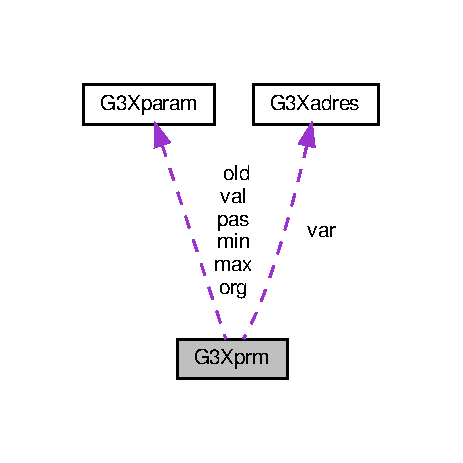
\includegraphics[width=222pt]{struct_g3_xprm__coll__graph}
\end{center}
\end{figure}
\subsection*{Data Fields}
\begin{DoxyCompactItemize}
\item 
char \hyperlink{struct_g3_xprm_a855b08d072a849c277e92b629e3eaddb}{ope}
\item 
char \hyperlink{struct_g3_xprm_a4e9b04711448362dbab666d433567f34}{nom} \mbox{[}16\mbox{]}
\item 
\hyperlink{struct_g3_xadres}{G3\+Xadres} \hyperlink{struct_g3_xprm_a354591d125c7cd20f2fcec10cdb15188}{var}
\item 
\hyperlink{struct_g3_xparam}{G3\+Xparam} \hyperlink{struct_g3_xprm_ab69882f819bf766798d589ebdcb88810}{pas}
\item 
\hyperlink{struct_g3_xparam}{G3\+Xparam} \hyperlink{struct_g3_xprm_a1e453f453193191f86ef66743034a5e9}{min}
\item 
\hyperlink{struct_g3_xparam}{G3\+Xparam} \hyperlink{struct_g3_xprm_a254ef12f104f240e2c82a0f6850c1604}{max}
\item 
\hyperlink{struct_g3_xparam}{G3\+Xparam} \hyperlink{struct_g3_xprm_a47d33e71270284b7a2894e05d2e027f1}{org}
\item 
\hyperlink{struct_g3_xparam}{G3\+Xparam} \hyperlink{struct_g3_xprm_a4d4fb5e18a33888fe4983e76456c66c9}{val}
\item 
\hyperlink{struct_g3_xparam}{G3\+Xparam} \hyperlink{struct_g3_xprm_a5d42b0a6c39faee9e535f8e14181e26c}{old}
\end{DoxyCompactItemize}


\subsection{Field Documentation}
\mbox{\Hypertarget{struct_g3_xprm_a254ef12f104f240e2c82a0f6850c1604}\label{struct_g3_xprm_a254ef12f104f240e2c82a0f6850c1604}} 
\index{G3\+Xprm@{G3\+Xprm}!max@{max}}
\index{max@{max}!G3\+Xprm@{G3\+Xprm}}
\subsubsection{\texorpdfstring{max}{max}}
{\footnotesize\ttfamily \hyperlink{struct_g3_xparam}{G3\+Xparam} max}

\mbox{\Hypertarget{struct_g3_xprm_a1e453f453193191f86ef66743034a5e9}\label{struct_g3_xprm_a1e453f453193191f86ef66743034a5e9}} 
\index{G3\+Xprm@{G3\+Xprm}!min@{min}}
\index{min@{min}!G3\+Xprm@{G3\+Xprm}}
\subsubsection{\texorpdfstring{min}{min}}
{\footnotesize\ttfamily \hyperlink{struct_g3_xparam}{G3\+Xparam} min}

\mbox{\Hypertarget{struct_g3_xprm_a4e9b04711448362dbab666d433567f34}\label{struct_g3_xprm_a4e9b04711448362dbab666d433567f34}} 
\index{G3\+Xprm@{G3\+Xprm}!nom@{nom}}
\index{nom@{nom}!G3\+Xprm@{G3\+Xprm}}
\subsubsection{\texorpdfstring{nom}{nom}}
{\footnotesize\ttfamily char nom\mbox{[}16\mbox{]}}

\mbox{\Hypertarget{struct_g3_xprm_a5d42b0a6c39faee9e535f8e14181e26c}\label{struct_g3_xprm_a5d42b0a6c39faee9e535f8e14181e26c}} 
\index{G3\+Xprm@{G3\+Xprm}!old@{old}}
\index{old@{old}!G3\+Xprm@{G3\+Xprm}}
\subsubsection{\texorpdfstring{old}{old}}
{\footnotesize\ttfamily \hyperlink{struct_g3_xparam}{G3\+Xparam} old}

\mbox{\Hypertarget{struct_g3_xprm_a855b08d072a849c277e92b629e3eaddb}\label{struct_g3_xprm_a855b08d072a849c277e92b629e3eaddb}} 
\index{G3\+Xprm@{G3\+Xprm}!ope@{ope}}
\index{ope@{ope}!G3\+Xprm@{G3\+Xprm}}
\subsubsection{\texorpdfstring{ope}{ope}}
{\footnotesize\ttfamily char ope}

\mbox{\Hypertarget{struct_g3_xprm_a47d33e71270284b7a2894e05d2e027f1}\label{struct_g3_xprm_a47d33e71270284b7a2894e05d2e027f1}} 
\index{G3\+Xprm@{G3\+Xprm}!org@{org}}
\index{org@{org}!G3\+Xprm@{G3\+Xprm}}
\subsubsection{\texorpdfstring{org}{org}}
{\footnotesize\ttfamily \hyperlink{struct_g3_xparam}{G3\+Xparam} org}

\mbox{\Hypertarget{struct_g3_xprm_ab69882f819bf766798d589ebdcb88810}\label{struct_g3_xprm_ab69882f819bf766798d589ebdcb88810}} 
\index{G3\+Xprm@{G3\+Xprm}!pas@{pas}}
\index{pas@{pas}!G3\+Xprm@{G3\+Xprm}}
\subsubsection{\texorpdfstring{pas}{pas}}
{\footnotesize\ttfamily \hyperlink{struct_g3_xparam}{G3\+Xparam} pas}

\mbox{\Hypertarget{struct_g3_xprm_a4d4fb5e18a33888fe4983e76456c66c9}\label{struct_g3_xprm_a4d4fb5e18a33888fe4983e76456c66c9}} 
\index{G3\+Xprm@{G3\+Xprm}!val@{val}}
\index{val@{val}!G3\+Xprm@{G3\+Xprm}}
\subsubsection{\texorpdfstring{val}{val}}
{\footnotesize\ttfamily \hyperlink{struct_g3_xparam}{G3\+Xparam} val}

\mbox{\Hypertarget{struct_g3_xprm_a354591d125c7cd20f2fcec10cdb15188}\label{struct_g3_xprm_a354591d125c7cd20f2fcec10cdb15188}} 
\index{G3\+Xprm@{G3\+Xprm}!var@{var}}
\index{var@{var}!G3\+Xprm@{G3\+Xprm}}
\subsubsection{\texorpdfstring{var}{var}}
{\footnotesize\ttfamily \hyperlink{struct_g3_xadres}{G3\+Xadres} var}



The documentation for this struct was generated from the following file\+:\begin{DoxyCompactItemize}
\item 
libg3x/src/\hyperlink{g3x__ctrlprm_8c}{g3x\+\_\+ctrlprm.\+c}\end{DoxyCompactItemize}

\hypertarget{struct_g3_xquat}{}\section{G3\+Xquat Struct Reference}
\label{struct_g3_xquat}\index{G3\+Xquat@{G3\+Xquat}}


{\ttfamily \#include $<$g3x\+\_\+quaternions.\+h$>$}

\subsection*{Data Fields}
\begin{DoxyCompactItemize}
\item 
\hyperlink{g3x__transfo_8h_a89b2b23e407882a535d835574a7912e1}{double} \hyperlink{struct_g3_xquat_a880a49112fedae68e714341a9a082fb6}{r}
\item 
\hyperlink{g3x__types_8h_a6181ad7c7bac1d7942ab3944bae2b8a1}{G3\+Xvector} \hyperlink{struct_g3_xquat_a26230cbe52f1aebedaea5628686a643b}{v}
\end{DoxyCompactItemize}


\subsection{Field Documentation}
\mbox{\Hypertarget{struct_g3_xquat_a880a49112fedae68e714341a9a082fb6}\label{struct_g3_xquat_a880a49112fedae68e714341a9a082fb6}} 
\index{G3\+Xquat@{G3\+Xquat}!r@{r}}
\index{r@{r}!G3\+Xquat@{G3\+Xquat}}
\subsubsection{\texorpdfstring{r}{r}}
{\footnotesize\ttfamily \hyperlink{g3x__transfo_8h_a89b2b23e407882a535d835574a7912e1}{double} r}

\mbox{\Hypertarget{struct_g3_xquat_a26230cbe52f1aebedaea5628686a643b}\label{struct_g3_xquat_a26230cbe52f1aebedaea5628686a643b}} 
\index{G3\+Xquat@{G3\+Xquat}!v@{v}}
\index{v@{v}!G3\+Xquat@{G3\+Xquat}}
\subsubsection{\texorpdfstring{v}{v}}
{\footnotesize\ttfamily \hyperlink{g3x__types_8h_a6181ad7c7bac1d7942ab3944bae2b8a1}{G3\+Xvector} v}



The documentation for this struct was generated from the following file\+:\begin{DoxyCompactItemize}
\item 
libg3x/include/\hyperlink{g3x__quaternions_8h}{g3x\+\_\+quaternions.\+h}\end{DoxyCompactItemize}

\hypertarget{struct_g3_xscroll}{}\section{G3\+Xscroll Struct Reference}
\label{struct_g3_xscroll}\index{G3\+Xscroll@{G3\+Xscroll}}
\subsection*{Data Fields}
\begin{DoxyCompactItemize}
\item 
\hyperlink{g3x__transfo_8h_a89b2b23e407882a535d835574a7912e1}{double} \hyperlink{struct_g3_xscroll_aac2416dd901b6711b49b1bad640462fa}{cursor}
\item 
\hyperlink{g3x__transfo_8h_a89b2b23e407882a535d835574a7912e1}{double} \hyperlink{struct_g3_xscroll_aad36546e8175d2922bee165fe028fedc}{min}
\item 
\hyperlink{g3x__transfo_8h_a89b2b23e407882a535d835574a7912e1}{double} \hyperlink{struct_g3_xscroll_a0b0ede69e8156eb97acc579b88e883de}{max}
\item 
\hyperlink{g3x__transfo_8h_a89b2b23e407882a535d835574a7912e1}{double} \hyperlink{struct_g3_xscroll_ae061d397826cfa2de10dbf4d39e45c2b}{fac}
\item 
\hyperlink{g3x__transfo_8h_a89b2b23e407882a535d835574a7912e1}{double} $\ast$ \hyperlink{struct_g3_xscroll_a6e0310455a4985ffbf39653fdee20a8a}{dprm}
\item 
int $\ast$ \hyperlink{struct_g3_xscroll_ac10925eeb681dafd5c6761bd51b25eca}{iprm}
\item 
int \hyperlink{struct_g3_xscroll_a924c1eb707e0db1173fe6a04f2ac67d4}{xcurs}
\item 
int \hyperlink{struct_g3_xscroll_a8a7bbcc9998fba42cea9ea3803cd99d4}{ycurs}
\item 
int \hyperlink{struct_g3_xscroll_aac374e320caaadeca4874add33b62af2}{w}
\item 
int \hyperlink{struct_g3_xscroll_a7441ef0865bcb3db9b8064dd7375c1ea}{id}
\item 
char \hyperlink{struct_g3_xscroll_aaf1bd07e95aeff0f585394fccaf479ab}{name} \mbox{[}8\mbox{]}
\item 
char \hyperlink{struct_g3_xscroll_aef383a8ccd6a48889b57cb6ceb7091f6}{info} \mbox{[}128\mbox{]}
\end{DoxyCompactItemize}


\subsection{Field Documentation}
\mbox{\Hypertarget{struct_g3_xscroll_aac2416dd901b6711b49b1bad640462fa}\label{struct_g3_xscroll_aac2416dd901b6711b49b1bad640462fa}} 
\index{G3\+Xscroll@{G3\+Xscroll}!cursor@{cursor}}
\index{cursor@{cursor}!G3\+Xscroll@{G3\+Xscroll}}
\subsubsection{\texorpdfstring{cursor}{cursor}}
{\footnotesize\ttfamily \hyperlink{g3x__transfo_8h_a89b2b23e407882a535d835574a7912e1}{double} cursor}

\mbox{\Hypertarget{struct_g3_xscroll_a6e0310455a4985ffbf39653fdee20a8a}\label{struct_g3_xscroll_a6e0310455a4985ffbf39653fdee20a8a}} 
\index{G3\+Xscroll@{G3\+Xscroll}!dprm@{dprm}}
\index{dprm@{dprm}!G3\+Xscroll@{G3\+Xscroll}}
\subsubsection{\texorpdfstring{dprm}{dprm}}
{\footnotesize\ttfamily \hyperlink{g3x__transfo_8h_a89b2b23e407882a535d835574a7912e1}{double}$\ast$ dprm}

\mbox{\Hypertarget{struct_g3_xscroll_ae061d397826cfa2de10dbf4d39e45c2b}\label{struct_g3_xscroll_ae061d397826cfa2de10dbf4d39e45c2b}} 
\index{G3\+Xscroll@{G3\+Xscroll}!fac@{fac}}
\index{fac@{fac}!G3\+Xscroll@{G3\+Xscroll}}
\subsubsection{\texorpdfstring{fac}{fac}}
{\footnotesize\ttfamily \hyperlink{g3x__transfo_8h_a89b2b23e407882a535d835574a7912e1}{double} fac}

\mbox{\Hypertarget{struct_g3_xscroll_a7441ef0865bcb3db9b8064dd7375c1ea}\label{struct_g3_xscroll_a7441ef0865bcb3db9b8064dd7375c1ea}} 
\index{G3\+Xscroll@{G3\+Xscroll}!id@{id}}
\index{id@{id}!G3\+Xscroll@{G3\+Xscroll}}
\subsubsection{\texorpdfstring{id}{id}}
{\footnotesize\ttfamily int id}

\mbox{\Hypertarget{struct_g3_xscroll_aef383a8ccd6a48889b57cb6ceb7091f6}\label{struct_g3_xscroll_aef383a8ccd6a48889b57cb6ceb7091f6}} 
\index{G3\+Xscroll@{G3\+Xscroll}!info@{info}}
\index{info@{info}!G3\+Xscroll@{G3\+Xscroll}}
\subsubsection{\texorpdfstring{info}{info}}
{\footnotesize\ttfamily char info\mbox{[}128\mbox{]}}

\mbox{\Hypertarget{struct_g3_xscroll_ac10925eeb681dafd5c6761bd51b25eca}\label{struct_g3_xscroll_ac10925eeb681dafd5c6761bd51b25eca}} 
\index{G3\+Xscroll@{G3\+Xscroll}!iprm@{iprm}}
\index{iprm@{iprm}!G3\+Xscroll@{G3\+Xscroll}}
\subsubsection{\texorpdfstring{iprm}{iprm}}
{\footnotesize\ttfamily int$\ast$ iprm}

\mbox{\Hypertarget{struct_g3_xscroll_a0b0ede69e8156eb97acc579b88e883de}\label{struct_g3_xscroll_a0b0ede69e8156eb97acc579b88e883de}} 
\index{G3\+Xscroll@{G3\+Xscroll}!max@{max}}
\index{max@{max}!G3\+Xscroll@{G3\+Xscroll}}
\subsubsection{\texorpdfstring{max}{max}}
{\footnotesize\ttfamily \hyperlink{g3x__transfo_8h_a89b2b23e407882a535d835574a7912e1}{double} max}

\mbox{\Hypertarget{struct_g3_xscroll_aad36546e8175d2922bee165fe028fedc}\label{struct_g3_xscroll_aad36546e8175d2922bee165fe028fedc}} 
\index{G3\+Xscroll@{G3\+Xscroll}!min@{min}}
\index{min@{min}!G3\+Xscroll@{G3\+Xscroll}}
\subsubsection{\texorpdfstring{min}{min}}
{\footnotesize\ttfamily \hyperlink{g3x__transfo_8h_a89b2b23e407882a535d835574a7912e1}{double} min}

\mbox{\Hypertarget{struct_g3_xscroll_aaf1bd07e95aeff0f585394fccaf479ab}\label{struct_g3_xscroll_aaf1bd07e95aeff0f585394fccaf479ab}} 
\index{G3\+Xscroll@{G3\+Xscroll}!name@{name}}
\index{name@{name}!G3\+Xscroll@{G3\+Xscroll}}
\subsubsection{\texorpdfstring{name}{name}}
{\footnotesize\ttfamily char name\mbox{[}8\mbox{]}}

\mbox{\Hypertarget{struct_g3_xscroll_aac374e320caaadeca4874add33b62af2}\label{struct_g3_xscroll_aac374e320caaadeca4874add33b62af2}} 
\index{G3\+Xscroll@{G3\+Xscroll}!w@{w}}
\index{w@{w}!G3\+Xscroll@{G3\+Xscroll}}
\subsubsection{\texorpdfstring{w}{w}}
{\footnotesize\ttfamily int w}

\mbox{\Hypertarget{struct_g3_xscroll_a924c1eb707e0db1173fe6a04f2ac67d4}\label{struct_g3_xscroll_a924c1eb707e0db1173fe6a04f2ac67d4}} 
\index{G3\+Xscroll@{G3\+Xscroll}!xcurs@{xcurs}}
\index{xcurs@{xcurs}!G3\+Xscroll@{G3\+Xscroll}}
\subsubsection{\texorpdfstring{xcurs}{xcurs}}
{\footnotesize\ttfamily int xcurs}

\mbox{\Hypertarget{struct_g3_xscroll_a8a7bbcc9998fba42cea9ea3803cd99d4}\label{struct_g3_xscroll_a8a7bbcc9998fba42cea9ea3803cd99d4}} 
\index{G3\+Xscroll@{G3\+Xscroll}!ycurs@{ycurs}}
\index{ycurs@{ycurs}!G3\+Xscroll@{G3\+Xscroll}}
\subsubsection{\texorpdfstring{ycurs}{ycurs}}
{\footnotesize\ttfamily int ycurs}



The documentation for this struct was generated from the following file\+:\begin{DoxyCompactItemize}
\item 
libg3x/src/\hyperlink{g3x__scroll_8c}{g3x\+\_\+scroll.\+c}\end{DoxyCompactItemize}

\hypertarget{struct_g3_xswitch}{}\section{G3\+Xswitch Struct Reference}
\label{struct_g3_xswitch}\index{G3\+Xswitch@{G3\+Xswitch}}
\subsection*{Data Fields}
\begin{DoxyCompactItemize}
\item 
int \hyperlink{struct_g3_xswitch_a86cf672daa4e0ad11ad10efc894d19c8}{num}
\item 
int \hyperlink{struct_g3_xswitch_a6150e0515f7202e2fb518f7206ed97dc}{x}
\item 
int \hyperlink{struct_g3_xswitch_a0a2f84ed7838f07779ae24c5a9086d33}{y}
\item 
int \hyperlink{struct_g3_xswitch_afed088663f8704004425cdae2120b9b3}{len}
\item 
char \hyperlink{struct_g3_xswitch_aa998d085055b9e9634ea1781cc0163c7}{name} \mbox{[}\hyperlink{g3x__switch_8c_a0e40ba0c0da54aafd8c34999455ec4fa}{M\+A\+X\+B\+U\+T\+L\+EN}+1\mbox{]}
\item 
char \hyperlink{struct_g3_xswitch_aef383a8ccd6a48889b57cb6ceb7091f6}{info} \mbox{[}128\mbox{]}
\item 
\hyperlink{g3x__types_8h_af6a258d8f3ee5206d682d799316314b1}{bool} $\ast$ \hyperlink{struct_g3_xswitch_a16a9b47d5bb16c05344c6601f74e24cf}{flag}
\end{DoxyCompactItemize}


\subsection{Field Documentation}
\mbox{\Hypertarget{struct_g3_xswitch_a16a9b47d5bb16c05344c6601f74e24cf}\label{struct_g3_xswitch_a16a9b47d5bb16c05344c6601f74e24cf}} 
\index{G3\+Xswitch@{G3\+Xswitch}!flag@{flag}}
\index{flag@{flag}!G3\+Xswitch@{G3\+Xswitch}}
\subsubsection{\texorpdfstring{flag}{flag}}
{\footnotesize\ttfamily \hyperlink{g3x__types_8h_af6a258d8f3ee5206d682d799316314b1}{bool}$\ast$ flag}

\mbox{\Hypertarget{struct_g3_xswitch_aef383a8ccd6a48889b57cb6ceb7091f6}\label{struct_g3_xswitch_aef383a8ccd6a48889b57cb6ceb7091f6}} 
\index{G3\+Xswitch@{G3\+Xswitch}!info@{info}}
\index{info@{info}!G3\+Xswitch@{G3\+Xswitch}}
\subsubsection{\texorpdfstring{info}{info}}
{\footnotesize\ttfamily char info\mbox{[}128\mbox{]}}

\mbox{\Hypertarget{struct_g3_xswitch_afed088663f8704004425cdae2120b9b3}\label{struct_g3_xswitch_afed088663f8704004425cdae2120b9b3}} 
\index{G3\+Xswitch@{G3\+Xswitch}!len@{len}}
\index{len@{len}!G3\+Xswitch@{G3\+Xswitch}}
\subsubsection{\texorpdfstring{len}{len}}
{\footnotesize\ttfamily int len}

\mbox{\Hypertarget{struct_g3_xswitch_aa998d085055b9e9634ea1781cc0163c7}\label{struct_g3_xswitch_aa998d085055b9e9634ea1781cc0163c7}} 
\index{G3\+Xswitch@{G3\+Xswitch}!name@{name}}
\index{name@{name}!G3\+Xswitch@{G3\+Xswitch}}
\subsubsection{\texorpdfstring{name}{name}}
{\footnotesize\ttfamily char name\mbox{[}\hyperlink{g3x__switch_8c_a0e40ba0c0da54aafd8c34999455ec4fa}{M\+A\+X\+B\+U\+T\+L\+EN}+1\mbox{]}}

\mbox{\Hypertarget{struct_g3_xswitch_a86cf672daa4e0ad11ad10efc894d19c8}\label{struct_g3_xswitch_a86cf672daa4e0ad11ad10efc894d19c8}} 
\index{G3\+Xswitch@{G3\+Xswitch}!num@{num}}
\index{num@{num}!G3\+Xswitch@{G3\+Xswitch}}
\subsubsection{\texorpdfstring{num}{num}}
{\footnotesize\ttfamily int num}

\mbox{\Hypertarget{struct_g3_xswitch_a6150e0515f7202e2fb518f7206ed97dc}\label{struct_g3_xswitch_a6150e0515f7202e2fb518f7206ed97dc}} 
\index{G3\+Xswitch@{G3\+Xswitch}!x@{x}}
\index{x@{x}!G3\+Xswitch@{G3\+Xswitch}}
\subsubsection{\texorpdfstring{x}{x}}
{\footnotesize\ttfamily int x}

\mbox{\Hypertarget{struct_g3_xswitch_a0a2f84ed7838f07779ae24c5a9086d33}\label{struct_g3_xswitch_a0a2f84ed7838f07779ae24c5a9086d33}} 
\index{G3\+Xswitch@{G3\+Xswitch}!y@{y}}
\index{y@{y}!G3\+Xswitch@{G3\+Xswitch}}
\subsubsection{\texorpdfstring{y}{y}}
{\footnotesize\ttfamily int y}



The documentation for this struct was generated from the following file\+:\begin{DoxyCompactItemize}
\item 
libg3x/src/\hyperlink{g3x__switch_8c}{g3x\+\_\+switch.\+c}\end{DoxyCompactItemize}

\hypertarget{struct_image}{}\section{Image Struct Reference}
\label{struct_image}\index{Image@{Image}}


represents an \hyperlink{struct_image}{Image}  




{\ttfamily \#include $<$Image.\+h$>$}



Collaboration diagram for Image\+:\nopagebreak
\begin{figure}[H]
\begin{center}
\leavevmode
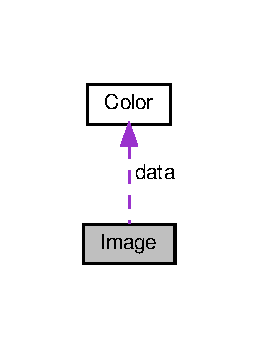
\includegraphics[width=124pt]{struct_image__coll__graph}
\end{center}
\end{figure}
\subsection*{Data Fields}
\begin{DoxyCompactItemize}
\item 
int \hyperlink{struct_image_aac374e320caaadeca4874add33b62af2}{w}
\item 
int \hyperlink{struct_image_a16611451551e3d15916bae723c3f59f7}{h}
\item 
\hyperlink{struct_color}{Color} $\ast$ \hyperlink{struct_image_a17c37489ef67e6333577cec67951bc7e}{data}
\end{DoxyCompactItemize}


\subsection{Detailed Description}
represents an \hyperlink{struct_image}{Image} 

\hyperlink{struct_image}{Image} is a type representing R\+GB \hyperlink{struct_image}{Image} 

\subsection{Field Documentation}
\mbox{\Hypertarget{struct_image_a17c37489ef67e6333577cec67951bc7e}\label{struct_image_a17c37489ef67e6333577cec67951bc7e}} 
\index{Image@{Image}!data@{data}}
\index{data@{data}!Image@{Image}}
\subsubsection{\texorpdfstring{data}{data}}
{\footnotesize\ttfamily \hyperlink{struct_color}{Color}$\ast$ data}

data of the image (pixel colors) \mbox{\Hypertarget{struct_image_a16611451551e3d15916bae723c3f59f7}\label{struct_image_a16611451551e3d15916bae723c3f59f7}} 
\index{Image@{Image}!h@{h}}
\index{h@{h}!Image@{Image}}
\subsubsection{\texorpdfstring{h}{h}}
{\footnotesize\ttfamily int h}

the height of the image \mbox{\Hypertarget{struct_image_aac374e320caaadeca4874add33b62af2}\label{struct_image_aac374e320caaadeca4874add33b62af2}} 
\index{Image@{Image}!w@{w}}
\index{w@{w}!Image@{Image}}
\subsubsection{\texorpdfstring{w}{w}}
{\footnotesize\ttfamily int w}

the width of the image 

The documentation for this struct was generated from the following file\+:\begin{DoxyCompactItemize}
\item 
include/\hyperlink{_image_8h}{Image.\+h}\end{DoxyCompactItemize}

\hypertarget{structlst__obj}{}\section{lst\+\_\+obj Struct Reference}
\label{structlst__obj}\index{lst\+\_\+obj@{lst\+\_\+obj}}


a list of objects to generate  




\subsection{Detailed Description}
a list of objects to generate 

a list of objects to generate 

The documentation for this struct was generated from the following file\+:\begin{DoxyCompactItemize}
\item 
\hyperlink{_scene__generator_8c}{Scene\+\_\+generator.\+c}\end{DoxyCompactItemize}

\hypertarget{structlst___object}{}\section{lst\+\_\+\+Object Struct Reference}
\label{structlst___object}\index{lst\+\_\+\+Object@{lst\+\_\+\+Object}}


a list of objects  




{\ttfamily \#include $<$Lst\+\_\+\+Object.\+h$>$}



\subsection{Detailed Description}
a list of objects 

a list of objects 

The documentation for this struct was generated from the following file\+:\begin{DoxyCompactItemize}
\item 
include/\hyperlink{_lst___object_8h}{Lst\+\_\+\+Object.\+h}\end{DoxyCompactItemize}

\hypertarget{structlst___source}{}\section{lst\+\_\+\+Source Struct Reference}
\label{structlst___source}\index{lst\+\_\+\+Source@{lst\+\_\+\+Source}}


a liste of light sources  




{\ttfamily \#include $<$Light.\+h$>$}



\subsection{Detailed Description}
a liste of light sources 

The documentation for this struct was generated from the following file\+:\begin{DoxyCompactItemize}
\item 
include/\hyperlink{_light_8h}{Light.\+h}\end{DoxyCompactItemize}

\hypertarget{struct_object}{}\section{Object Struct Reference}
\label{struct_object}\index{Object@{Object}}


an object  




{\ttfamily \#include $<$Object.\+h$>$}



Collaboration diagram for Object\+:\nopagebreak
\begin{figure}[H]
\begin{center}
\leavevmode
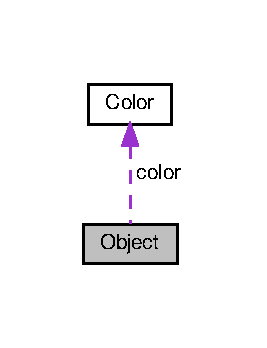
\includegraphics[width=128pt]{struct_object__coll__graph}
\end{center}
\end{figure}
\subsection*{Data Fields}
\begin{DoxyCompactItemize}
\item 
\hyperlink{_object_8h_af3ec464aa442c2d0bd0c227fda28a8be}{T\+Y\+P\+E\+\_\+\+O\+B\+J\+E\+CT} \hyperlink{struct_object_a19f6ed1bac9f5cab449a607abca42685}{canonique}
\item 
int \hyperlink{struct_object_ac8b96df3945daad611d0e916baf3fd33}{shininess}
\item 
\hyperlink{struct_color}{Color} \hyperlink{struct_object_aa5f4d1eda21c196bd8401ff73f105073}{color}
\item 
\hyperlink{g3x__transfo_8h_a89b2b23e407882a535d835574a7912e1}{double} \hyperlink{struct_object_a7b9fa288e1cec876534bd6f5b17aa049}{specular\+\_\+reflection\+\_\+coeff} \mbox{[}3\mbox{]}
\item 
\hyperlink{g3x__transfo_8h_a89b2b23e407882a535d835574a7912e1}{double} \hyperlink{struct_object_a365382686d7b8904ca564cd7745a7dbe}{diffuse\+\_\+reflection\+\_\+coeff} \mbox{[}3\mbox{]}
\item 
int($\ast$ \hyperlink{struct_object_a3f68899f8db0dc480e823d27163e1639}{rayon\+\_\+inter} )(const \hyperlink{struct_point}{Point} $\ast$A, const \hyperlink{struct_vecteur}{Vecteur} $\ast$u, \hyperlink{struct_point}{Point} $\ast$I, \hyperlink{struct_vecteur}{Vecteur} $\ast$N)
\item 
\hyperlink{_hmat_8h_a7263a9d077d77f58425e01446b766c9f}{Hmat} \hyperlink{struct_object_a2e39a1b3b70d4fad8a907b217ef63f59}{Md}
\item 
\hyperlink{_hmat_8h_a7263a9d077d77f58425e01446b766c9f}{Hmat} \hyperlink{struct_object_ab0efdf841b049d1b6f42f1c6c28a9557}{Mi}
\item 
\hyperlink{_hmat_8h_a7263a9d077d77f58425e01446b766c9f}{Hmat} \hyperlink{struct_object_a377e7ee9e852999ea0e10c66d74ddfb4}{Mn}
\end{DoxyCompactItemize}


\subsection{Detailed Description}
an object 

\hyperlink{struct_object}{Object} is a type representing a shape 

\subsection{Field Documentation}
\mbox{\Hypertarget{struct_object_a19f6ed1bac9f5cab449a607abca42685}\label{struct_object_a19f6ed1bac9f5cab449a607abca42685}} 
\index{Object@{Object}!canonique@{canonique}}
\index{canonique@{canonique}!Object@{Object}}
\subsubsection{\texorpdfstring{canonique}{canonique}}
{\footnotesize\ttfamily \hyperlink{_object_8h_af3ec464aa442c2d0bd0c227fda28a8be}{T\+Y\+P\+E\+\_\+\+O\+B\+J\+E\+CT} canonique}

reference to the canonical object \mbox{\Hypertarget{struct_object_aa5f4d1eda21c196bd8401ff73f105073}\label{struct_object_aa5f4d1eda21c196bd8401ff73f105073}} 
\index{Object@{Object}!color@{color}}
\index{color@{color}!Object@{Object}}
\subsubsection{\texorpdfstring{color}{color}}
{\footnotesize\ttfamily \hyperlink{struct_color}{Color} color}

R\+GB color \mbox{\Hypertarget{struct_object_a365382686d7b8904ca564cd7745a7dbe}\label{struct_object_a365382686d7b8904ca564cd7745a7dbe}} 
\index{Object@{Object}!diffuse\+\_\+reflection\+\_\+coeff@{diffuse\+\_\+reflection\+\_\+coeff}}
\index{diffuse\+\_\+reflection\+\_\+coeff@{diffuse\+\_\+reflection\+\_\+coeff}!Object@{Object}}
\subsubsection{\texorpdfstring{diffuse\+\_\+reflection\+\_\+coeff}{diffuse\_reflection\_coeff}}
{\footnotesize\ttfamily \hyperlink{g3x__transfo_8h_a89b2b23e407882a535d835574a7912e1}{double} diffuse\+\_\+reflection\+\_\+coeff\mbox{[}3\mbox{]}}

R\+GB coefficient between 0 and 1 \mbox{\Hypertarget{struct_object_a2e39a1b3b70d4fad8a907b217ef63f59}\label{struct_object_a2e39a1b3b70d4fad8a907b217ef63f59}} 
\index{Object@{Object}!Md@{Md}}
\index{Md@{Md}!Object@{Object}}
\subsubsection{\texorpdfstring{Md}{Md}}
{\footnotesize\ttfamily \hyperlink{_hmat_8h_a7263a9d077d77f58425e01446b766c9f}{Hmat} Md}

\mbox{\Hypertarget{struct_object_ab0efdf841b049d1b6f42f1c6c28a9557}\label{struct_object_ab0efdf841b049d1b6f42f1c6c28a9557}} 
\index{Object@{Object}!Mi@{Mi}}
\index{Mi@{Mi}!Object@{Object}}
\subsubsection{\texorpdfstring{Mi}{Mi}}
{\footnotesize\ttfamily \hyperlink{_hmat_8h_a7263a9d077d77f58425e01446b766c9f}{Hmat} Mi}

\mbox{\Hypertarget{struct_object_a377e7ee9e852999ea0e10c66d74ddfb4}\label{struct_object_a377e7ee9e852999ea0e10c66d74ddfb4}} 
\index{Object@{Object}!Mn@{Mn}}
\index{Mn@{Mn}!Object@{Object}}
\subsubsection{\texorpdfstring{Mn}{Mn}}
{\footnotesize\ttfamily \hyperlink{_hmat_8h_a7263a9d077d77f58425e01446b766c9f}{Hmat} Mn}

direct, inverse and normal homogeneous matrices \mbox{\Hypertarget{struct_object_a3f68899f8db0dc480e823d27163e1639}\label{struct_object_a3f68899f8db0dc480e823d27163e1639}} 
\index{Object@{Object}!rayon\+\_\+inter@{rayon\+\_\+inter}}
\index{rayon\+\_\+inter@{rayon\+\_\+inter}!Object@{Object}}
\subsubsection{\texorpdfstring{rayon\+\_\+inter}{rayon\_inter}}
{\footnotesize\ttfamily int($\ast$ rayon\+\_\+inter) (const \hyperlink{struct_point}{Point} $\ast$A, const \hyperlink{struct_vecteur}{Vecteur} $\ast$u, \hyperlink{struct_point}{Point} $\ast$I, \hyperlink{struct_vecteur}{Vecteur} $\ast$N)}

1 if the object is seen from point A, 0 otherwise \mbox{\Hypertarget{struct_object_ac8b96df3945daad611d0e916baf3fd33}\label{struct_object_ac8b96df3945daad611d0e916baf3fd33}} 
\index{Object@{Object}!shininess@{shininess}}
\index{shininess@{shininess}!Object@{Object}}
\subsubsection{\texorpdfstring{shininess}{shininess}}
{\footnotesize\ttfamily int shininess}

value between 2 and 256 \mbox{\Hypertarget{struct_object_a7b9fa288e1cec876534bd6f5b17aa049}\label{struct_object_a7b9fa288e1cec876534bd6f5b17aa049}} 
\index{Object@{Object}!specular\+\_\+reflection\+\_\+coeff@{specular\+\_\+reflection\+\_\+coeff}}
\index{specular\+\_\+reflection\+\_\+coeff@{specular\+\_\+reflection\+\_\+coeff}!Object@{Object}}
\subsubsection{\texorpdfstring{specular\+\_\+reflection\+\_\+coeff}{specular\_reflection\_coeff}}
{\footnotesize\ttfamily \hyperlink{g3x__transfo_8h_a89b2b23e407882a535d835574a7912e1}{double} specular\+\_\+reflection\+\_\+coeff\mbox{[}3\mbox{]}}

R\+GB coefficient between 0 and 1 

The documentation for this struct was generated from the following file\+:\begin{DoxyCompactItemize}
\item 
include/\hyperlink{_object_8h}{Object.\+h}\end{DoxyCompactItemize}

\hypertarget{struct_option}{}\section{Option Struct Reference}
\label{struct_option}\index{Option@{Option}}


options specified by the user  




{\ttfamily \#include $<$Option.\+h$>$}

\subsection*{Data Fields}
\begin{DoxyCompactItemize}
\item 
int \hyperlink{struct_option_acf4d33ee4cff36f69b924471174dcb11}{level}
\item 
int \hyperlink{struct_option_a55a22286c25bb0d604e9425da1c0c121}{timer\+\_\+on\+\_\+compute\+\_\+scene}
\item 
int \hyperlink{struct_option_ad7146066ca84f44322c4b8b9b0cf68b3}{pixel\+\_\+sampling}
\item 
char $\ast$ \hyperlink{struct_option_ae034085e87d427c78144ccce961ee56f}{input\+\_\+path}
\item 
char $\ast$ \hyperlink{struct_option_a73c330e3842fe255aa5e7d82bf573289}{output\+\_\+path}
\end{DoxyCompactItemize}


\subsection{Detailed Description}
options specified by the user 

options specified by the user 

\subsection{Field Documentation}
\mbox{\Hypertarget{struct_option_ae034085e87d427c78144ccce961ee56f}\label{struct_option_ae034085e87d427c78144ccce961ee56f}} 
\index{Option@{Option}!input\+\_\+path@{input\+\_\+path}}
\index{input\+\_\+path@{input\+\_\+path}!Option@{Option}}
\subsubsection{\texorpdfstring{input\+\_\+path}{input\_path}}
{\footnotesize\ttfamily char$\ast$ input\+\_\+path}

the path to the scene to import \mbox{\Hypertarget{struct_option_acf4d33ee4cff36f69b924471174dcb11}\label{struct_option_acf4d33ee4cff36f69b924471174dcb11}} 
\index{Option@{Option}!level@{level}}
\index{level@{level}!Option@{Option}}
\subsubsection{\texorpdfstring{level}{level}}
{\footnotesize\ttfamily int level}

the level of scene wanted by the user \mbox{\Hypertarget{struct_option_a73c330e3842fe255aa5e7d82bf573289}\label{struct_option_a73c330e3842fe255aa5e7d82bf573289}} 
\index{Option@{Option}!output\+\_\+path@{output\+\_\+path}}
\index{output\+\_\+path@{output\+\_\+path}!Option@{Option}}
\subsubsection{\texorpdfstring{output\+\_\+path}{output\_path}}
{\footnotesize\ttfamily char$\ast$ output\+\_\+path}

the path of the exported image \mbox{\Hypertarget{struct_option_ad7146066ca84f44322c4b8b9b0cf68b3}\label{struct_option_ad7146066ca84f44322c4b8b9b0cf68b3}} 
\index{Option@{Option}!pixel\+\_\+sampling@{pixel\+\_\+sampling}}
\index{pixel\+\_\+sampling@{pixel\+\_\+sampling}!Option@{Option}}
\subsubsection{\texorpdfstring{pixel\+\_\+sampling}{pixel\_sampling}}
{\footnotesize\ttfamily int pixel\+\_\+sampling}

the number of pixel sampling \mbox{\Hypertarget{struct_option_a55a22286c25bb0d604e9425da1c0c121}\label{struct_option_a55a22286c25bb0d604e9425da1c0c121}} 
\index{Option@{Option}!timer\+\_\+on\+\_\+compute\+\_\+scene@{timer\+\_\+on\+\_\+compute\+\_\+scene}}
\index{timer\+\_\+on\+\_\+compute\+\_\+scene@{timer\+\_\+on\+\_\+compute\+\_\+scene}!Option@{Option}}
\subsubsection{\texorpdfstring{timer\+\_\+on\+\_\+compute\+\_\+scene}{timer\_on\_compute\_scene}}
{\footnotesize\ttfamily int timer\+\_\+on\+\_\+compute\+\_\+scene}

if the user wants to time the compute scene 

The documentation for this struct was generated from the following file\+:\begin{DoxyCompactItemize}
\item 
include/\hyperlink{_option_8h}{Option.\+h}\end{DoxyCompactItemize}

\hypertarget{structpng__t}{}\section{png\+\_\+t Struct Reference}
\label{structpng__t}\index{png\+\_\+t@{png\+\_\+t}}


a type representing a png image  


\subsection*{Data Fields}
\begin{DoxyCompactItemize}
\item 
size\+\_\+t \hyperlink{structpng__t_ad721fc6ca6a3d6ba3bc506576622aab0}{capacity}
\item 
char $\ast$ \hyperlink{structpng__t_a91a70b77df95bd8b0830b49a094c2acb}{data}
\item 
size\+\_\+t \hyperlink{structpng__t_a02bed8590a9ddf520e58a060059518ec}{width}
\item 
size\+\_\+t \hyperlink{structpng__t_a02afeaaf8574e7a78d6b466ff2695052}{height}
\item 
char $\ast$ \hyperlink{structpng__t_a392d7ef877b6258e64850ce3a2647dae}{out}
\item 
size\+\_\+t \hyperlink{structpng__t_ac8ef22a87f97ef02768e0faedea1307d}{out\+\_\+pos}
\item 
size\+\_\+t \hyperlink{structpng__t_ac8fcf2b31db62e2bfeb7c2ee10b39908}{out\+\_\+capacity}
\item 
uint32\+\_\+t \hyperlink{structpng__t_a85b7a7f21b6108b69872839e2509cd67}{crc}
\item 
uint16\+\_\+t \hyperlink{structpng__t_a90256a2c1ea2d035ef0a2b87e543bcb8}{s1}
\item 
uint16\+\_\+t \hyperlink{structpng__t_a95ac0a163ca4077eac153ae972bfae9f}{s2}
\item 
size\+\_\+t \hyperlink{structpng__t_a1b190a6d9d3ec163d1a9547740e5d6eb}{bpp}
\item 
size\+\_\+t \hyperlink{structpng__t_aac2e70794d77a569d02e9db38669f145}{stream\+\_\+x}
\item 
size\+\_\+t \hyperlink{structpng__t_a7b8b9225ada455d197dee07a4a25b910}{stream\+\_\+y}
\end{DoxyCompactItemize}


\subsection{Detailed Description}
a type representing a png image 

a type representing a png image 

\subsection{Field Documentation}
\mbox{\Hypertarget{structpng__t_a1b190a6d9d3ec163d1a9547740e5d6eb}\label{structpng__t_a1b190a6d9d3ec163d1a9547740e5d6eb}} 
\index{png\+\_\+t@{png\+\_\+t}!bpp@{bpp}}
\index{bpp@{bpp}!png\+\_\+t@{png\+\_\+t}}
\subsubsection{\texorpdfstring{bpp}{bpp}}
{\footnotesize\ttfamily size\+\_\+t bpp}

Bytes per pixel \mbox{\Hypertarget{structpng__t_ad721fc6ca6a3d6ba3bc506576622aab0}\label{structpng__t_ad721fc6ca6a3d6ba3bc506576622aab0}} 
\index{png\+\_\+t@{png\+\_\+t}!capacity@{capacity}}
\index{capacity@{capacity}!png\+\_\+t@{png\+\_\+t}}
\subsubsection{\texorpdfstring{capacity}{capacity}}
{\footnotesize\ttfamily size\+\_\+t capacity}

Reserved memory for raw data \mbox{\Hypertarget{structpng__t_a85b7a7f21b6108b69872839e2509cd67}\label{structpng__t_a85b7a7f21b6108b69872839e2509cd67}} 
\index{png\+\_\+t@{png\+\_\+t}!crc@{crc}}
\index{crc@{crc}!png\+\_\+t@{png\+\_\+t}}
\subsubsection{\texorpdfstring{crc}{crc}}
{\footnotesize\ttfamily uint32\+\_\+t crc}

Current C\+R\+C32 checksum \mbox{\Hypertarget{structpng__t_a91a70b77df95bd8b0830b49a094c2acb}\label{structpng__t_a91a70b77df95bd8b0830b49a094c2acb}} 
\index{png\+\_\+t@{png\+\_\+t}!data@{data}}
\index{data@{data}!png\+\_\+t@{png\+\_\+t}}
\subsubsection{\texorpdfstring{data}{data}}
{\footnotesize\ttfamily char$\ast$ data}

Raw pixel data, format depends on type \mbox{\Hypertarget{structpng__t_a02afeaaf8574e7a78d6b466ff2695052}\label{structpng__t_a02afeaaf8574e7a78d6b466ff2695052}} 
\index{png\+\_\+t@{png\+\_\+t}!height@{height}}
\index{height@{height}!png\+\_\+t@{png\+\_\+t}}
\subsubsection{\texorpdfstring{height}{height}}
{\footnotesize\ttfamily size\+\_\+t height}

\hyperlink{struct_image}{Image} height \mbox{\Hypertarget{structpng__t_a392d7ef877b6258e64850ce3a2647dae}\label{structpng__t_a392d7ef877b6258e64850ce3a2647dae}} 
\index{png\+\_\+t@{png\+\_\+t}!out@{out}}
\index{out@{out}!png\+\_\+t@{png\+\_\+t}}
\subsubsection{\texorpdfstring{out}{out}}
{\footnotesize\ttfamily char$\ast$ out}

Buffer to store final P\+NG \mbox{\Hypertarget{structpng__t_ac8fcf2b31db62e2bfeb7c2ee10b39908}\label{structpng__t_ac8fcf2b31db62e2bfeb7c2ee10b39908}} 
\index{png\+\_\+t@{png\+\_\+t}!out\+\_\+capacity@{out\+\_\+capacity}}
\index{out\+\_\+capacity@{out\+\_\+capacity}!png\+\_\+t@{png\+\_\+t}}
\subsubsection{\texorpdfstring{out\+\_\+capacity}{out\_capacity}}
{\footnotesize\ttfamily size\+\_\+t out\+\_\+capacity}

Capacity of output buffer \mbox{\Hypertarget{structpng__t_ac8ef22a87f97ef02768e0faedea1307d}\label{structpng__t_ac8ef22a87f97ef02768e0faedea1307d}} 
\index{png\+\_\+t@{png\+\_\+t}!out\+\_\+pos@{out\+\_\+pos}}
\index{out\+\_\+pos@{out\+\_\+pos}!png\+\_\+t@{png\+\_\+t}}
\subsubsection{\texorpdfstring{out\+\_\+pos}{out\_pos}}
{\footnotesize\ttfamily size\+\_\+t out\+\_\+pos}

Current size of output buffer \mbox{\Hypertarget{structpng__t_a90256a2c1ea2d035ef0a2b87e543bcb8}\label{structpng__t_a90256a2c1ea2d035ef0a2b87e543bcb8}} 
\index{png\+\_\+t@{png\+\_\+t}!s1@{s1}}
\index{s1@{s1}!png\+\_\+t@{png\+\_\+t}}
\subsubsection{\texorpdfstring{s1}{s1}}
{\footnotesize\ttfamily uint16\+\_\+t s1}

Helper variables for Adler checksum \mbox{\Hypertarget{structpng__t_a95ac0a163ca4077eac153ae972bfae9f}\label{structpng__t_a95ac0a163ca4077eac153ae972bfae9f}} 
\index{png\+\_\+t@{png\+\_\+t}!s2@{s2}}
\index{s2@{s2}!png\+\_\+t@{png\+\_\+t}}
\subsubsection{\texorpdfstring{s2}{s2}}
{\footnotesize\ttfamily uint16\+\_\+t s2}

Helper variables for Adler checksum \mbox{\Hypertarget{structpng__t_aac2e70794d77a569d02e9db38669f145}\label{structpng__t_aac2e70794d77a569d02e9db38669f145}} 
\index{png\+\_\+t@{png\+\_\+t}!stream\+\_\+x@{stream\+\_\+x}}
\index{stream\+\_\+x@{stream\+\_\+x}!png\+\_\+t@{png\+\_\+t}}
\subsubsection{\texorpdfstring{stream\+\_\+x}{stream\_x}}
{\footnotesize\ttfamily size\+\_\+t stream\+\_\+x}

Current x coordinate for pixel streaming \mbox{\Hypertarget{structpng__t_a7b8b9225ada455d197dee07a4a25b910}\label{structpng__t_a7b8b9225ada455d197dee07a4a25b910}} 
\index{png\+\_\+t@{png\+\_\+t}!stream\+\_\+y@{stream\+\_\+y}}
\index{stream\+\_\+y@{stream\+\_\+y}!png\+\_\+t@{png\+\_\+t}}
\subsubsection{\texorpdfstring{stream\+\_\+y}{stream\_y}}
{\footnotesize\ttfamily size\+\_\+t stream\+\_\+y}

Current y coordinate for pixel streaming \mbox{\Hypertarget{structpng__t_a02bed8590a9ddf520e58a060059518ec}\label{structpng__t_a02bed8590a9ddf520e58a060059518ec}} 
\index{png\+\_\+t@{png\+\_\+t}!width@{width}}
\index{width@{width}!png\+\_\+t@{png\+\_\+t}}
\subsubsection{\texorpdfstring{width}{width}}
{\footnotesize\ttfamily size\+\_\+t width}

\hyperlink{struct_image}{Image} width 

The documentation for this struct was generated from the following file\+:\begin{DoxyCompactItemize}
\item 
src/\hyperlink{_png___output_8c}{Png\+\_\+\+Output.\+c}\end{DoxyCompactItemize}

\hypertarget{struct_point}{}\section{Point Struct Reference}
\label{struct_point}\index{Point@{Point}}


a point in 3D space  




{\ttfamily \#include $<$Point.\+h$>$}

\subsection*{Data Fields}
\begin{DoxyCompactItemize}
\item 
\hyperlink{g3x__transfo_8h_a89b2b23e407882a535d835574a7912e1}{double} \hyperlink{struct_point_af88b946fb90d5f08b5fb740c70e98c10}{x}
\item 
\hyperlink{g3x__transfo_8h_a89b2b23e407882a535d835574a7912e1}{double} \hyperlink{struct_point_ab927965981178aa1fba979a37168db2a}{y}
\item 
\hyperlink{g3x__transfo_8h_a89b2b23e407882a535d835574a7912e1}{double} \hyperlink{struct_point_ab3e6ed577a7c669c19de1f9c1b46c872}{z}
\end{DoxyCompactItemize}


\subsection{Detailed Description}
a point in 3D space 

\hyperlink{struct_point}{Point} is a type representing a point by its three real coordinates 

\subsection{Field Documentation}
\mbox{\Hypertarget{struct_point_af88b946fb90d5f08b5fb740c70e98c10}\label{struct_point_af88b946fb90d5f08b5fb740c70e98c10}} 
\index{Point@{Point}!x@{x}}
\index{x@{x}!Point@{Point}}
\subsubsection{\texorpdfstring{x}{x}}
{\footnotesize\ttfamily \hyperlink{g3x__transfo_8h_a89b2b23e407882a535d835574a7912e1}{double} x}

\mbox{\Hypertarget{struct_point_ab927965981178aa1fba979a37168db2a}\label{struct_point_ab927965981178aa1fba979a37168db2a}} 
\index{Point@{Point}!y@{y}}
\index{y@{y}!Point@{Point}}
\subsubsection{\texorpdfstring{y}{y}}
{\footnotesize\ttfamily \hyperlink{g3x__transfo_8h_a89b2b23e407882a535d835574a7912e1}{double} y}

\mbox{\Hypertarget{struct_point_ab3e6ed577a7c669c19de1f9c1b46c872}\label{struct_point_ab3e6ed577a7c669c19de1f9c1b46c872}} 
\index{Point@{Point}!z@{z}}
\index{z@{z}!Point@{Point}}
\subsubsection{\texorpdfstring{z}{z}}
{\footnotesize\ttfamily \hyperlink{g3x__transfo_8h_a89b2b23e407882a535d835574a7912e1}{double} z}



The documentation for this struct was generated from the following file\+:\begin{DoxyCompactItemize}
\item 
include/\hyperlink{_point_8h}{Point.\+h}\end{DoxyCompactItemize}

\hypertarget{struct_rectangle}{}\section{Rectangle Struct Reference}
\label{struct_rectangle}\index{Rectangle@{Rectangle}}


a rectangle  




{\ttfamily \#include $<$Rectangle.\+h$>$}



Collaboration diagram for Rectangle\+:\nopagebreak
\begin{figure}[H]
\begin{center}
\leavevmode
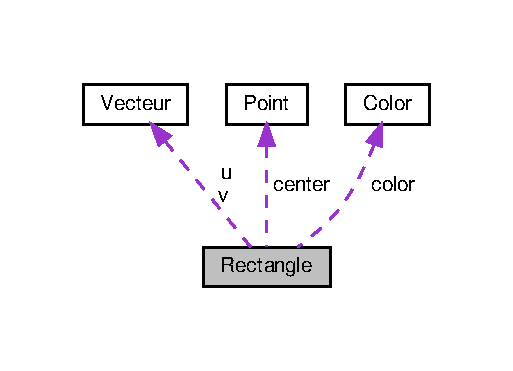
\includegraphics[width=246pt]{struct_rectangle__coll__graph}
\end{center}
\end{figure}
\subsection*{Data Fields}
\begin{DoxyCompactItemize}
\item 
\hyperlink{struct_color}{Color} \hyperlink{struct_rectangle_aa5f4d1eda21c196bd8401ff73f105073}{color}
\item 
\hyperlink{g3x__transfo_8h_a89b2b23e407882a535d835574a7912e1}{double} \hyperlink{struct_rectangle_a2459aedac9f8646ad9566164a9a83f41}{rayon}
\item 
\hyperlink{struct_point}{Point} \hyperlink{struct_rectangle_a24bb1c337bce91dd3e7a4a4372b11793}{center}
\item 
\hyperlink{struct_vecteur}{Vecteur} \hyperlink{struct_rectangle_a5aa1600754aceabfee725fb390410687}{u}
\item 
\hyperlink{struct_vecteur}{Vecteur} \hyperlink{struct_rectangle_a5ff420022374621dd6186970680c7276}{v}
\end{DoxyCompactItemize}


\subsection{Detailed Description}
a rectangle 

\hyperlink{struct_rectangle}{Rectangle} is a type representing a rectangle by its center, its raduis and an angle (u, v) which defines the plane of the rectangle and the other angles 

\subsection{Field Documentation}
\mbox{\Hypertarget{struct_rectangle_a24bb1c337bce91dd3e7a4a4372b11793}\label{struct_rectangle_a24bb1c337bce91dd3e7a4a4372b11793}} 
\index{Rectangle@{Rectangle}!center@{center}}
\index{center@{center}!Rectangle@{Rectangle}}
\subsubsection{\texorpdfstring{center}{center}}
{\footnotesize\ttfamily \hyperlink{struct_point}{Point} center}

\mbox{\Hypertarget{struct_rectangle_aa5f4d1eda21c196bd8401ff73f105073}\label{struct_rectangle_aa5f4d1eda21c196bd8401ff73f105073}} 
\index{Rectangle@{Rectangle}!color@{color}}
\index{color@{color}!Rectangle@{Rectangle}}
\subsubsection{\texorpdfstring{color}{color}}
{\footnotesize\ttfamily \hyperlink{struct_color}{Color} color}

\mbox{\Hypertarget{struct_rectangle_a2459aedac9f8646ad9566164a9a83f41}\label{struct_rectangle_a2459aedac9f8646ad9566164a9a83f41}} 
\index{Rectangle@{Rectangle}!rayon@{rayon}}
\index{rayon@{rayon}!Rectangle@{Rectangle}}
\subsubsection{\texorpdfstring{rayon}{rayon}}
{\footnotesize\ttfamily \hyperlink{g3x__transfo_8h_a89b2b23e407882a535d835574a7912e1}{double} rayon}

the distance from the center to an end point \mbox{\Hypertarget{struct_rectangle_a5aa1600754aceabfee725fb390410687}\label{struct_rectangle_a5aa1600754aceabfee725fb390410687}} 
\index{Rectangle@{Rectangle}!u@{u}}
\index{u@{u}!Rectangle@{Rectangle}}
\subsubsection{\texorpdfstring{u}{u}}
{\footnotesize\ttfamily \hyperlink{struct_vecteur}{Vecteur} u}

\mbox{\Hypertarget{struct_rectangle_a5ff420022374621dd6186970680c7276}\label{struct_rectangle_a5ff420022374621dd6186970680c7276}} 
\index{Rectangle@{Rectangle}!v@{v}}
\index{v@{v}!Rectangle@{Rectangle}}
\subsubsection{\texorpdfstring{v}{v}}
{\footnotesize\ttfamily \hyperlink{struct_vecteur}{Vecteur} v}



The documentation for this struct was generated from the following file\+:\begin{DoxyCompactItemize}
\item 
include/\hyperlink{_rectangle_8h}{Rectangle.\+h}\end{DoxyCompactItemize}

\hypertarget{struct_scene}{}\section{Scene Struct Reference}
\label{struct_scene}\index{Scene@{Scene}}


the 3D scene seen by the camera  




{\ttfamily \#include $<$Scene.\+h$>$}



Collaboration diagram for Scene\+:\nopagebreak
\begin{figure}[H]
\begin{center}
\leavevmode
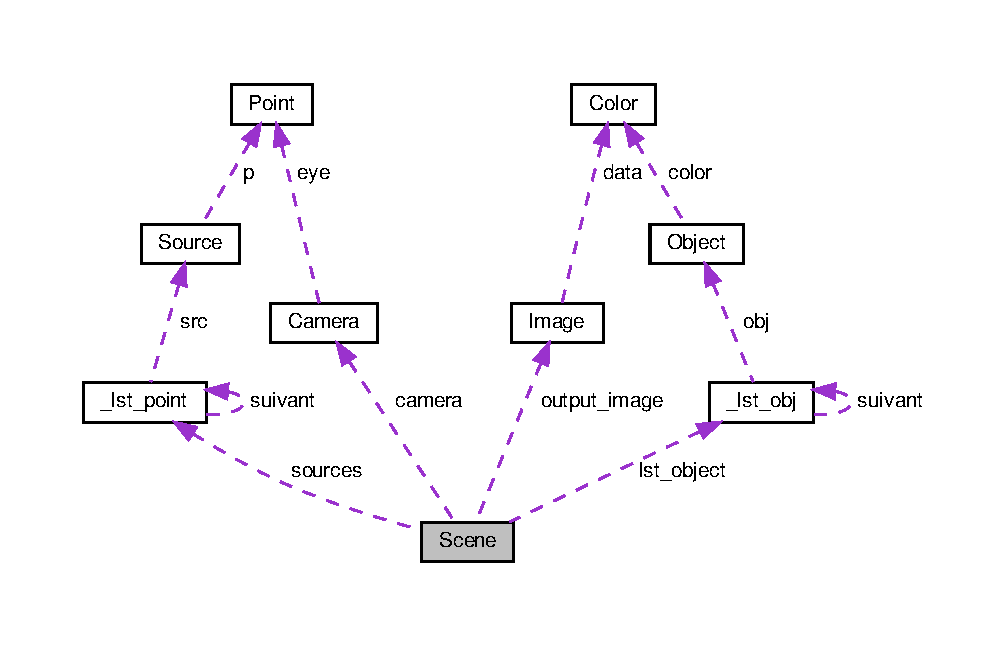
\includegraphics[width=350pt]{struct_scene__coll__graph}
\end{center}
\end{figure}
\subsection*{Data Fields}
\begin{DoxyCompactItemize}
\item 
int \hyperlink{struct_scene_acf4d33ee4cff36f69b924471174dcb11}{level}
\item 
int \hyperlink{struct_scene_ab42fe399d3a5afbb011869e914bdb51e}{reflection\+\_\+level}
\item 
int \hyperlink{struct_scene_a55a22286c25bb0d604e9425da1c0c121}{timer\+\_\+on\+\_\+compute\+\_\+scene}
\item 
int \hyperlink{struct_scene_ad7146066ca84f44322c4b8b9b0cf68b3}{pixel\+\_\+sampling}
\item 
int \hyperlink{struct_scene_a413744f68ce61704d543f5a8920f0d49}{count\+\_\+rayon}
\item 
\hyperlink{structlst___source}{lst\+\_\+\+Source} \hyperlink{struct_scene_af2cbe3867b855ed9935538ebfffe3a6f}{sources}
\item 
\hyperlink{struct_camera}{Camera} \hyperlink{struct_scene_a2008f4ab70b5e4104c2ca43932536ddf}{camera}
\item 
\hyperlink{structlst___object}{lst\+\_\+\+Object} \hyperlink{struct_scene_ad1a9dde1f53b5136da8ba5fd10417eb5}{lst\+\_\+object}
\item 
\hyperlink{struct_image}{Image} $\ast$ \hyperlink{struct_scene_a00c31761980e6dadd21455e3f21926da}{output\+\_\+image}
\end{DoxyCompactItemize}


\subsection{Detailed Description}
the 3D scene seen by the camera 

\hyperlink{struct_scene}{Scene} is a type representing a scene and all his components (shapes, lights, camera...) 

\subsection{Field Documentation}
\mbox{\Hypertarget{struct_scene_a2008f4ab70b5e4104c2ca43932536ddf}\label{struct_scene_a2008f4ab70b5e4104c2ca43932536ddf}} 
\index{Scene@{Scene}!camera@{camera}}
\index{camera@{camera}!Scene@{Scene}}
\subsubsection{\texorpdfstring{camera}{camera}}
{\footnotesize\ttfamily \hyperlink{struct_camera}{Camera} camera}

the camera observing the scene \mbox{\Hypertarget{struct_scene_a413744f68ce61704d543f5a8920f0d49}\label{struct_scene_a413744f68ce61704d543f5a8920f0d49}} 
\index{Scene@{Scene}!count\+\_\+rayon@{count\+\_\+rayon}}
\index{count\+\_\+rayon@{count\+\_\+rayon}!Scene@{Scene}}
\subsubsection{\texorpdfstring{count\+\_\+rayon}{count\_rayon}}
{\footnotesize\ttfamily int count\+\_\+rayon}

index (between 0 and 8) of the current ray launched in the given pixel (level 2) \mbox{\Hypertarget{struct_scene_acf4d33ee4cff36f69b924471174dcb11}\label{struct_scene_acf4d33ee4cff36f69b924471174dcb11}} 
\index{Scene@{Scene}!level@{level}}
\index{level@{level}!Scene@{Scene}}
\subsubsection{\texorpdfstring{level}{level}}
{\footnotesize\ttfamily int level}

the level can be 1, 2 or 3 \mbox{\Hypertarget{struct_scene_ad1a9dde1f53b5136da8ba5fd10417eb5}\label{struct_scene_ad1a9dde1f53b5136da8ba5fd10417eb5}} 
\index{Scene@{Scene}!lst\+\_\+object@{lst\+\_\+object}}
\index{lst\+\_\+object@{lst\+\_\+object}!Scene@{Scene}}
\subsubsection{\texorpdfstring{lst\+\_\+object}{lst\_object}}
{\footnotesize\ttfamily \hyperlink{structlst___object}{lst\+\_\+\+Object} lst\+\_\+object}

list of all objects \mbox{\Hypertarget{struct_scene_a00c31761980e6dadd21455e3f21926da}\label{struct_scene_a00c31761980e6dadd21455e3f21926da}} 
\index{Scene@{Scene}!output\+\_\+image@{output\+\_\+image}}
\index{output\+\_\+image@{output\+\_\+image}!Scene@{Scene}}
\subsubsection{\texorpdfstring{output\+\_\+image}{output\_image}}
{\footnotesize\ttfamily \hyperlink{struct_image}{Image}$\ast$ output\+\_\+image}

the computed image \mbox{\Hypertarget{struct_scene_ad7146066ca84f44322c4b8b9b0cf68b3}\label{struct_scene_ad7146066ca84f44322c4b8b9b0cf68b3}} 
\index{Scene@{Scene}!pixel\+\_\+sampling@{pixel\+\_\+sampling}}
\index{pixel\+\_\+sampling@{pixel\+\_\+sampling}!Scene@{Scene}}
\subsubsection{\texorpdfstring{pixel\+\_\+sampling}{pixel\_sampling}}
{\footnotesize\ttfamily int pixel\+\_\+sampling}

number of rays per pixel (level 3) \mbox{\Hypertarget{struct_scene_ab42fe399d3a5afbb011869e914bdb51e}\label{struct_scene_ab42fe399d3a5afbb011869e914bdb51e}} 
\index{Scene@{Scene}!reflection\+\_\+level@{reflection\+\_\+level}}
\index{reflection\+\_\+level@{reflection\+\_\+level}!Scene@{Scene}}
\subsubsection{\texorpdfstring{reflection\+\_\+level}{reflection\_level}}
{\footnotesize\ttfamily int reflection\+\_\+level}

the level of reflection of objects \mbox{\Hypertarget{struct_scene_af2cbe3867b855ed9935538ebfffe3a6f}\label{struct_scene_af2cbe3867b855ed9935538ebfffe3a6f}} 
\index{Scene@{Scene}!sources@{sources}}
\index{sources@{sources}!Scene@{Scene}}
\subsubsection{\texorpdfstring{sources}{sources}}
{\footnotesize\ttfamily \hyperlink{structlst___source}{lst\+\_\+\+Source} sources}

list of all light sources \mbox{\Hypertarget{struct_scene_a55a22286c25bb0d604e9425da1c0c121}\label{struct_scene_a55a22286c25bb0d604e9425da1c0c121}} 
\index{Scene@{Scene}!timer\+\_\+on\+\_\+compute\+\_\+scene@{timer\+\_\+on\+\_\+compute\+\_\+scene}}
\index{timer\+\_\+on\+\_\+compute\+\_\+scene@{timer\+\_\+on\+\_\+compute\+\_\+scene}!Scene@{Scene}}
\subsubsection{\texorpdfstring{timer\+\_\+on\+\_\+compute\+\_\+scene}{timer\_on\_compute\_scene}}
{\footnotesize\ttfamily int timer\+\_\+on\+\_\+compute\+\_\+scene}

if we have to time the scene calculation 

The documentation for this struct was generated from the following file\+:\begin{DoxyCompactItemize}
\item 
include/\hyperlink{_scene_8h}{Scene.\+h}\end{DoxyCompactItemize}

\hypertarget{struct_scene__info}{}\section{Scene\+\_\+info Struct Reference}
\label{struct_scene__info}\index{Scene\+\_\+info@{Scene\+\_\+info}}


all parameters desired by the user when generating the scene  




Collaboration diagram for Scene\+\_\+info\+:\nopagebreak
\begin{figure}[H]
\begin{center}
\leavevmode
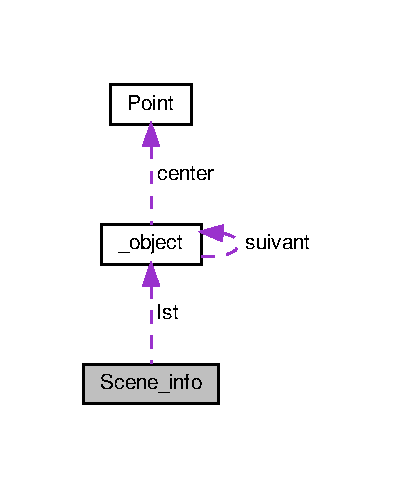
\includegraphics[width=190pt]{struct_scene__info__coll__graph}
\end{center}
\end{figure}
\subsection*{Data Fields}
\begin{DoxyCompactItemize}
\item 
unsigned int \hyperlink{struct_scene__info_a424ae246251dbf194cf480fd3b3eba60}{kind\+\_\+of\+\_\+object}
\item 
int \hyperlink{struct_scene__info_a432ce34b9fc8367bdfca15bee393de96}{tabulation\+\_\+nb}
\item 
int \hyperlink{struct_scene__info_a5a69c7addc967ed8dbc9da830e1ab534}{nb\+\_\+object}
\item 
int \hyperlink{struct_scene__info_a2474a5474cbff19523a51eb1de01cda4}{width}
\item 
int \hyperlink{struct_scene__info_ad12fc34ce789bce6c8a05d8a17138534}{height}
\item 
\hyperlink{structlst__obj}{lst\+\_\+obj} \hyperlink{struct_scene__info_ab9f02bcf7c8c98ddd57f47e4d8035ac6}{lst}
\item 
F\+I\+LE $\ast$ \hyperlink{struct_scene__info_a2960eb597f48f3b59bbb850b47e895ff}{output\+\_\+file}
\end{DoxyCompactItemize}


\subsection{Detailed Description}
all parameters desired by the user when generating the scene 

all parameters desired by the user when generating the scene 

\subsection{Field Documentation}
\mbox{\Hypertarget{struct_scene__info_ad12fc34ce789bce6c8a05d8a17138534}\label{struct_scene__info_ad12fc34ce789bce6c8a05d8a17138534}} 
\index{Scene\+\_\+info@{Scene\+\_\+info}!height@{height}}
\index{height@{height}!Scene\+\_\+info@{Scene\+\_\+info}}
\subsubsection{\texorpdfstring{height}{height}}
{\footnotesize\ttfamily int height}

the height of the scene when it will be exported in a image \mbox{\Hypertarget{struct_scene__info_a424ae246251dbf194cf480fd3b3eba60}\label{struct_scene__info_a424ae246251dbf194cf480fd3b3eba60}} 
\index{Scene\+\_\+info@{Scene\+\_\+info}!kind\+\_\+of\+\_\+object@{kind\+\_\+of\+\_\+object}}
\index{kind\+\_\+of\+\_\+object@{kind\+\_\+of\+\_\+object}!Scene\+\_\+info@{Scene\+\_\+info}}
\subsubsection{\texorpdfstring{kind\+\_\+of\+\_\+object}{kind\_of\_object}}
{\footnotesize\ttfamily unsigned int kind\+\_\+of\+\_\+object}

all kind of object \mbox{\Hypertarget{struct_scene__info_ab9f02bcf7c8c98ddd57f47e4d8035ac6}\label{struct_scene__info_ab9f02bcf7c8c98ddd57f47e4d8035ac6}} 
\index{Scene\+\_\+info@{Scene\+\_\+info}!lst@{lst}}
\index{lst@{lst}!Scene\+\_\+info@{Scene\+\_\+info}}
\subsubsection{\texorpdfstring{lst}{lst}}
{\footnotesize\ttfamily \hyperlink{structlst__obj}{lst\+\_\+obj} lst}

the list of objects to write in the file representing the scene \mbox{\Hypertarget{struct_scene__info_a5a69c7addc967ed8dbc9da830e1ab534}\label{struct_scene__info_a5a69c7addc967ed8dbc9da830e1ab534}} 
\index{Scene\+\_\+info@{Scene\+\_\+info}!nb\+\_\+object@{nb\+\_\+object}}
\index{nb\+\_\+object@{nb\+\_\+object}!Scene\+\_\+info@{Scene\+\_\+info}}
\subsubsection{\texorpdfstring{nb\+\_\+object}{nb\_object}}
{\footnotesize\ttfamily int nb\+\_\+object}

the number of objects to be generated \mbox{\Hypertarget{struct_scene__info_a2960eb597f48f3b59bbb850b47e895ff}\label{struct_scene__info_a2960eb597f48f3b59bbb850b47e895ff}} 
\index{Scene\+\_\+info@{Scene\+\_\+info}!output\+\_\+file@{output\+\_\+file}}
\index{output\+\_\+file@{output\+\_\+file}!Scene\+\_\+info@{Scene\+\_\+info}}
\subsubsection{\texorpdfstring{output\+\_\+file}{output\_file}}
{\footnotesize\ttfamily F\+I\+LE$\ast$ output\+\_\+file}

the output file containing the scene \mbox{\Hypertarget{struct_scene__info_a432ce34b9fc8367bdfca15bee393de96}\label{struct_scene__info_a432ce34b9fc8367bdfca15bee393de96}} 
\index{Scene\+\_\+info@{Scene\+\_\+info}!tabulation\+\_\+nb@{tabulation\+\_\+nb}}
\index{tabulation\+\_\+nb@{tabulation\+\_\+nb}!Scene\+\_\+info@{Scene\+\_\+info}}
\subsubsection{\texorpdfstring{tabulation\+\_\+nb}{tabulation\_nb}}
{\footnotesize\ttfamily int tabulation\+\_\+nb}

the number of times we need to tab (useful when creating the xml scene) \mbox{\Hypertarget{struct_scene__info_a2474a5474cbff19523a51eb1de01cda4}\label{struct_scene__info_a2474a5474cbff19523a51eb1de01cda4}} 
\index{Scene\+\_\+info@{Scene\+\_\+info}!width@{width}}
\index{width@{width}!Scene\+\_\+info@{Scene\+\_\+info}}
\subsubsection{\texorpdfstring{width}{width}}
{\footnotesize\ttfamily int width}

the width of the scene when it will be exported in a image 

The documentation for this struct was generated from the following file\+:\begin{DoxyCompactItemize}
\item 
\hyperlink{_scene__generator_8c}{Scene\+\_\+generator.\+c}\end{DoxyCompactItemize}

\hypertarget{struct_source}{}\section{Source Struct Reference}
\label{struct_source}\index{Source@{Source}}


a light source  




{\ttfamily \#include $<$Light.\+h$>$}



Collaboration diagram for Source\+:\nopagebreak
\begin{figure}[H]
\begin{center}
\leavevmode
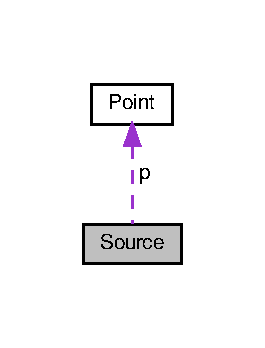
\includegraphics[width=127pt]{struct_source__coll__graph}
\end{center}
\end{figure}
\subsection*{Data Fields}
\begin{DoxyCompactItemize}
\item 
\hyperlink{g3x__transfo_8h_a89b2b23e407882a535d835574a7912e1}{double} \hyperlink{struct_source_a2118076db8e8f8a25c2376e1d4acfb67}{intensity}
\item 
\hyperlink{struct_point}{Point} \hyperlink{struct_source_ae273773add45375b65c8555736acb60f}{p}
\end{DoxyCompactItemize}


\subsection{Detailed Description}
a light source 

\hyperlink{struct_source}{Source} is a type representing a light source by its position in space and its intensity 

\subsection{Field Documentation}
\mbox{\Hypertarget{struct_source_a2118076db8e8f8a25c2376e1d4acfb67}\label{struct_source_a2118076db8e8f8a25c2376e1d4acfb67}} 
\index{Source@{Source}!intensity@{intensity}}
\index{intensity@{intensity}!Source@{Source}}
\subsubsection{\texorpdfstring{intensity}{intensity}}
{\footnotesize\ttfamily \hyperlink{g3x__transfo_8h_a89b2b23e407882a535d835574a7912e1}{double} intensity}

the intensity is a big value (millions) \mbox{\Hypertarget{struct_source_ae273773add45375b65c8555736acb60f}\label{struct_source_ae273773add45375b65c8555736acb60f}} 
\index{Source@{Source}!p@{p}}
\index{p@{p}!Source@{Source}}
\subsubsection{\texorpdfstring{p}{p}}
{\footnotesize\ttfamily \hyperlink{struct_point}{Point} p}

the position of the light source 

The documentation for this struct was generated from the following file\+:\begin{DoxyCompactItemize}
\item 
include/\hyperlink{_light_8h}{Light.\+h}\end{DoxyCompactItemize}

\hypertarget{struct_sphere}{}\section{Sphere Struct Reference}
\label{struct_sphere}\index{Sphere@{Sphere}}


a sphere  




{\ttfamily \#include $<$Sphere.\+h$>$}



Collaboration diagram for Sphere\+:\nopagebreak
\begin{figure}[H]
\begin{center}
\leavevmode
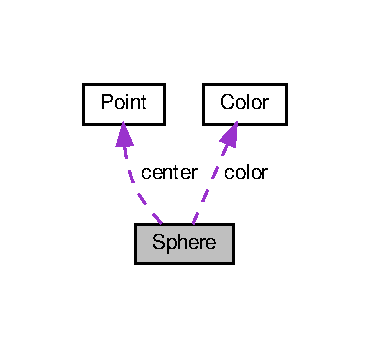
\includegraphics[width=178pt]{struct_sphere__coll__graph}
\end{center}
\end{figure}
\subsection*{Data Fields}
\begin{DoxyCompactItemize}
\item 
\hyperlink{struct_color}{Color} \hyperlink{struct_sphere_aa5f4d1eda21c196bd8401ff73f105073}{color}
\item 
\hyperlink{g3x__transfo_8h_a89b2b23e407882a535d835574a7912e1}{double} \hyperlink{struct_sphere_a2459aedac9f8646ad9566164a9a83f41}{rayon}
\item 
\hyperlink{struct_point}{Point} \hyperlink{struct_sphere_a24bb1c337bce91dd3e7a4a4372b11793}{center}
\end{DoxyCompactItemize}


\subsection{Detailed Description}
a sphere 

\hyperlink{struct_sphere}{Sphere} is a type representing a sphere by its center and its raduis 

\subsection{Field Documentation}
\mbox{\Hypertarget{struct_sphere_a24bb1c337bce91dd3e7a4a4372b11793}\label{struct_sphere_a24bb1c337bce91dd3e7a4a4372b11793}} 
\index{Sphere@{Sphere}!center@{center}}
\index{center@{center}!Sphere@{Sphere}}
\subsubsection{\texorpdfstring{center}{center}}
{\footnotesize\ttfamily \hyperlink{struct_point}{Point} center}

\mbox{\Hypertarget{struct_sphere_aa5f4d1eda21c196bd8401ff73f105073}\label{struct_sphere_aa5f4d1eda21c196bd8401ff73f105073}} 
\index{Sphere@{Sphere}!color@{color}}
\index{color@{color}!Sphere@{Sphere}}
\subsubsection{\texorpdfstring{color}{color}}
{\footnotesize\ttfamily \hyperlink{struct_color}{Color} color}

\mbox{\Hypertarget{struct_sphere_a2459aedac9f8646ad9566164a9a83f41}\label{struct_sphere_a2459aedac9f8646ad9566164a9a83f41}} 
\index{Sphere@{Sphere}!rayon@{rayon}}
\index{rayon@{rayon}!Sphere@{Sphere}}
\subsubsection{\texorpdfstring{rayon}{rayon}}
{\footnotesize\ttfamily \hyperlink{g3x__transfo_8h_a89b2b23e407882a535d835574a7912e1}{double} rayon}



The documentation for this struct was generated from the following file\+:\begin{DoxyCompactItemize}
\item 
include/\hyperlink{_sphere_8h}{Sphere.\+h}\end{DoxyCompactItemize}

\hypertarget{struct_triangle}{}\section{Triangle Struct Reference}
\label{struct_triangle}\index{Triangle@{Triangle}}


a triangle  




{\ttfamily \#include $<$Triangle.\+h$>$}



Collaboration diagram for Triangle\+:\nopagebreak
\begin{figure}[H]
\begin{center}
\leavevmode
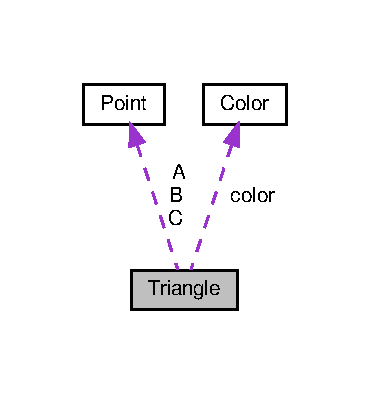
\includegraphics[width=178pt]{struct_triangle__coll__graph}
\end{center}
\end{figure}
\subsection*{Data Fields}
\begin{DoxyCompactItemize}
\item 
\hyperlink{struct_color}{Color} \hyperlink{struct_triangle_aa5f4d1eda21c196bd8401ff73f105073}{color}
\item 
\hyperlink{struct_point}{Point} \hyperlink{struct_triangle_a52df86c0a1979613c6b8ee0f785ba181}{A}
\item 
\hyperlink{struct_point}{Point} \hyperlink{struct_triangle_a42d857842a35fc7c3bfda0922ddcdd70}{B}
\item 
\hyperlink{struct_point}{Point} \hyperlink{struct_triangle_a3d8ff0c539667710e4db6c73b03dbc63}{C}
\end{DoxyCompactItemize}


\subsection{Detailed Description}
a triangle 

a triangle is defined by its three points 

\subsection{Field Documentation}
\mbox{\Hypertarget{struct_triangle_a52df86c0a1979613c6b8ee0f785ba181}\label{struct_triangle_a52df86c0a1979613c6b8ee0f785ba181}} 
\index{Triangle@{Triangle}!A@{A}}
\index{A@{A}!Triangle@{Triangle}}
\subsubsection{\texorpdfstring{A}{A}}
{\footnotesize\ttfamily \hyperlink{struct_point}{Point} A}

\mbox{\Hypertarget{struct_triangle_a42d857842a35fc7c3bfda0922ddcdd70}\label{struct_triangle_a42d857842a35fc7c3bfda0922ddcdd70}} 
\index{Triangle@{Triangle}!B@{B}}
\index{B@{B}!Triangle@{Triangle}}
\subsubsection{\texorpdfstring{B}{B}}
{\footnotesize\ttfamily \hyperlink{struct_point}{Point} B}

\mbox{\Hypertarget{struct_triangle_a3d8ff0c539667710e4db6c73b03dbc63}\label{struct_triangle_a3d8ff0c539667710e4db6c73b03dbc63}} 
\index{Triangle@{Triangle}!C@{C}}
\index{C@{C}!Triangle@{Triangle}}
\subsubsection{\texorpdfstring{C}{C}}
{\footnotesize\ttfamily \hyperlink{struct_point}{Point} C}

\mbox{\Hypertarget{struct_triangle_aa5f4d1eda21c196bd8401ff73f105073}\label{struct_triangle_aa5f4d1eda21c196bd8401ff73f105073}} 
\index{Triangle@{Triangle}!color@{color}}
\index{color@{color}!Triangle@{Triangle}}
\subsubsection{\texorpdfstring{color}{color}}
{\footnotesize\ttfamily \hyperlink{struct_color}{Color} color}



The documentation for this struct was generated from the following file\+:\begin{DoxyCompactItemize}
\item 
include/\hyperlink{_triangle_8h}{Triangle.\+h}\end{DoxyCompactItemize}

\hypertarget{struct_vecteur}{}\section{Vecteur Struct Reference}
\label{struct_vecteur}\index{Vecteur@{Vecteur}}


represents a vector in 3D space.  




{\ttfamily \#include $<$Vecteur.\+h$>$}

\subsection*{Data Fields}
\begin{DoxyCompactItemize}
\item 
\hyperlink{g3x__transfo_8h_a89b2b23e407882a535d835574a7912e1}{double} \hyperlink{struct_vecteur_af88b946fb90d5f08b5fb740c70e98c10}{x}
\item 
\hyperlink{g3x__transfo_8h_a89b2b23e407882a535d835574a7912e1}{double} \hyperlink{struct_vecteur_ab927965981178aa1fba979a37168db2a}{y}
\item 
\hyperlink{g3x__transfo_8h_a89b2b23e407882a535d835574a7912e1}{double} \hyperlink{struct_vecteur_ab3e6ed577a7c669c19de1f9c1b46c872}{z}
\end{DoxyCompactItemize}


\subsection{Detailed Description}
represents a vector in 3D space. 

\hyperlink{struct_vecteur}{Vecteur} is a type representing a vector in 3D space 

\subsection{Field Documentation}
\mbox{\Hypertarget{struct_vecteur_af88b946fb90d5f08b5fb740c70e98c10}\label{struct_vecteur_af88b946fb90d5f08b5fb740c70e98c10}} 
\index{Vecteur@{Vecteur}!x@{x}}
\index{x@{x}!Vecteur@{Vecteur}}
\subsubsection{\texorpdfstring{x}{x}}
{\footnotesize\ttfamily \hyperlink{g3x__transfo_8h_a89b2b23e407882a535d835574a7912e1}{double} x}

the x coordinate \mbox{\Hypertarget{struct_vecteur_ab927965981178aa1fba979a37168db2a}\label{struct_vecteur_ab927965981178aa1fba979a37168db2a}} 
\index{Vecteur@{Vecteur}!y@{y}}
\index{y@{y}!Vecteur@{Vecteur}}
\subsubsection{\texorpdfstring{y}{y}}
{\footnotesize\ttfamily \hyperlink{g3x__transfo_8h_a89b2b23e407882a535d835574a7912e1}{double} y}

the y coordinate \mbox{\Hypertarget{struct_vecteur_ab3e6ed577a7c669c19de1f9c1b46c872}\label{struct_vecteur_ab3e6ed577a7c669c19de1f9c1b46c872}} 
\index{Vecteur@{Vecteur}!z@{z}}
\index{z@{z}!Vecteur@{Vecteur}}
\subsubsection{\texorpdfstring{z}{z}}
{\footnotesize\ttfamily \hyperlink{g3x__transfo_8h_a89b2b23e407882a535d835574a7912e1}{double} z}

the z coordinate 

The documentation for this struct was generated from the following file\+:\begin{DoxyCompactItemize}
\item 
include/\hyperlink{_vecteur_8h}{Vecteur.\+h}\end{DoxyCompactItemize}

\chapter{File Documentation}
\hypertarget{_camera_8h}{}\section{include/\+Camera.h File Reference}
\label{_camera_8h}\index{include/\+Camera.\+h@{include/\+Camera.\+h}}


represents a camera filming the scene  


{\ttfamily \#include \char`\"{}Point.\+h\char`\"{}}\newline
{\ttfamily \#include \char`\"{}Hmat.\+h\char`\"{}}\newline
Include dependency graph for Camera.\+h\+:\nopagebreak
\begin{figure}[H]
\begin{center}
\leavevmode
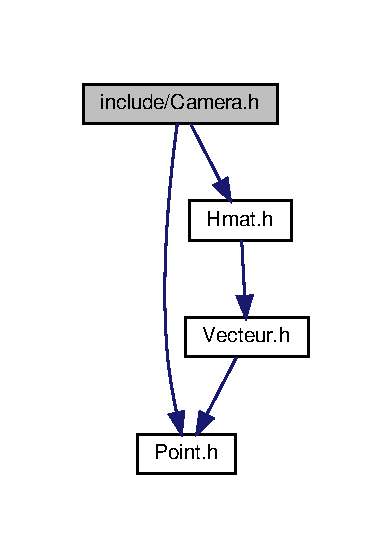
\includegraphics[width=188pt]{_camera_8h__incl}
\end{center}
\end{figure}
This graph shows which files directly or indirectly include this file\+:\nopagebreak
\begin{figure}[H]
\begin{center}
\leavevmode
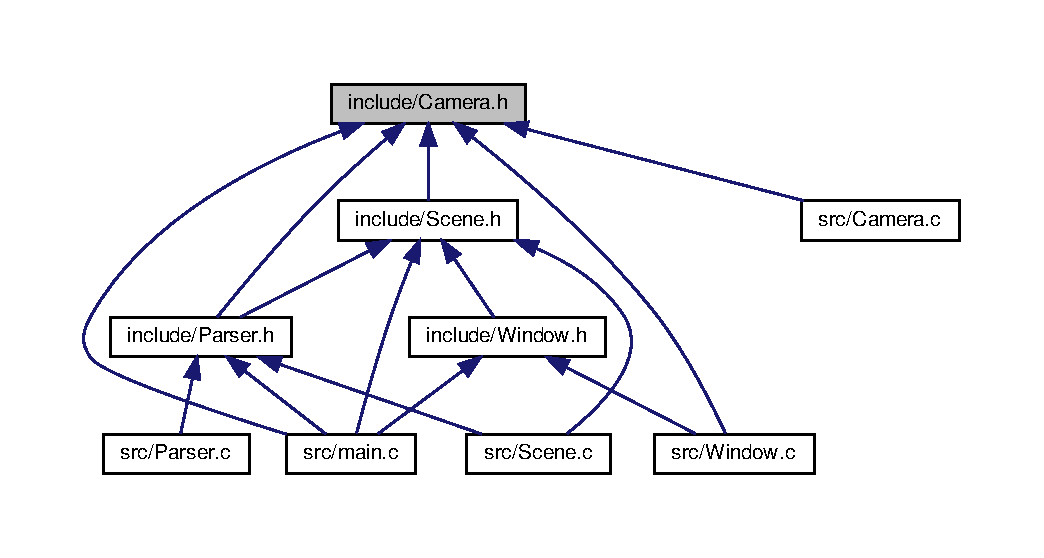
\includegraphics[width=350pt]{_camera_8h__dep__incl}
\end{center}
\end{figure}
\subsection*{Data Structures}
\begin{DoxyCompactItemize}
\item 
struct \hyperlink{struct_camera}{Camera}
\begin{DoxyCompactList}\small\item\em represents a camera observing the scene \end{DoxyCompactList}\end{DoxyCompactItemize}
\subsection*{Functions}
\begin{DoxyCompactItemize}
\item 
int \hyperlink{_camera_8h_a1db8aade6c98c0f35a24611a29418755}{set\+Camera} (\hyperlink{struct_camera}{Camera} $\ast$camera, const \hyperlink{struct_point}{Point} $\ast$eye, int resolution\mbox{[}2\mbox{]}, int screen\mbox{[}2\mbox{]})
\begin{DoxyCompactList}\small\item\em sets the camera with the specified values \end{DoxyCompactList}\item 
int \hyperlink{_camera_8h_a1d314288e23a95c99811e6955a57a71c}{Camera\+Console\+Display} (const \hyperlink{struct_camera}{Camera} $\ast$camera, int return\+\_\+line)
\begin{DoxyCompactList}\small\item\em print a camera in the console \end{DoxyCompactList}\end{DoxyCompactItemize}


\subsection{Detailed Description}
represents a camera filming the scene 

\begin{DoxyAuthor}{Author}
Jean-\/\+Manuel E\+R\+I\+A\+LC -\/ Hadjer D\+J\+E\+R\+R\+O\+U\+MI 
\end{DoxyAuthor}
\begin{DoxyVersion}{Version}
0.\+1 
\end{DoxyVersion}
\begin{DoxyDate}{Date}
11 juin 2020
\end{DoxyDate}
represents a camera filming the scene 

\subsection{Function Documentation}
\mbox{\Hypertarget{_camera_8h_a1d314288e23a95c99811e6955a57a71c}\label{_camera_8h_a1d314288e23a95c99811e6955a57a71c}} 
\index{Camera.\+h@{Camera.\+h}!Camera\+Console\+Display@{Camera\+Console\+Display}}
\index{Camera\+Console\+Display@{Camera\+Console\+Display}!Camera.\+h@{Camera.\+h}}
\subsubsection{\texorpdfstring{Camera\+Console\+Display()}{CameraConsoleDisplay()}}
{\footnotesize\ttfamily int Camera\+Console\+Display (\begin{DoxyParamCaption}\item[{const \hyperlink{struct_camera}{Camera} $\ast$}]{camera,  }\item[{int}]{return\+\_\+line }\end{DoxyParamCaption})}



print a camera in the console 


\begin{DoxyParams}{Parameters}
{\em camera} & the camera to print \\
\hline
{\em return\+\_\+line} & != 0 if we want to add a \textquotesingle{}~\newline
\textquotesingle{} after the print \\
\hline
\end{DoxyParams}
\begin{DoxyReturn}{Returns}
0 if a error occurs(camera == N\+U\+LL)~\newline
 1 otherwise 
\end{DoxyReturn}
\mbox{\Hypertarget{_camera_8h_a1db8aade6c98c0f35a24611a29418755}\label{_camera_8h_a1db8aade6c98c0f35a24611a29418755}} 
\index{Camera.\+h@{Camera.\+h}!set\+Camera@{set\+Camera}}
\index{set\+Camera@{set\+Camera}!Camera.\+h@{Camera.\+h}}
\subsubsection{\texorpdfstring{set\+Camera()}{setCamera()}}
{\footnotesize\ttfamily int set\+Camera (\begin{DoxyParamCaption}\item[{\hyperlink{struct_camera}{Camera} $\ast$}]{camera,  }\item[{const \hyperlink{struct_point}{Point} $\ast$}]{eye,  }\item[{int}]{resolution\mbox{[}2\mbox{]},  }\item[{int}]{screen\mbox{[}2\mbox{]} }\end{DoxyParamCaption})}



sets the camera with the specified values 


\begin{DoxyParams}{Parameters}
{\em camera} & the camera to change \\
\hline
{\em eye} & the new point of vue of the camera \\
\hline
{\em resolution} & the new resolution \\
\hline
{\em screen} & the dimensions of the new screen \\
\hline
\end{DoxyParams}
\begin{DoxyReturn}{Returns}
0 if a error occurs(one parameter is N\+U\+L\+L)~\newline
 1 otherwise 
\end{DoxyReturn}

\hypertarget{_color_8h}{}\section{include/\+Color.h File Reference}
\label{_color_8h}\index{include/\+Color.\+h@{include/\+Color.\+h}}


contains R\+GB color type and all functions related to it  


{\ttfamily \#include $<$stdint.\+h$>$}\newline
Include dependency graph for Color.\+h\+:\nopagebreak
\begin{figure}[H]
\begin{center}
\leavevmode
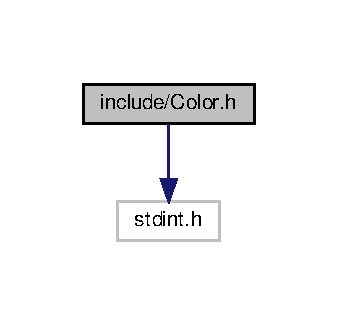
\includegraphics[width=162pt]{_color_8h__incl}
\end{center}
\end{figure}
This graph shows which files directly or indirectly include this file\+:\nopagebreak
\begin{figure}[H]
\begin{center}
\leavevmode
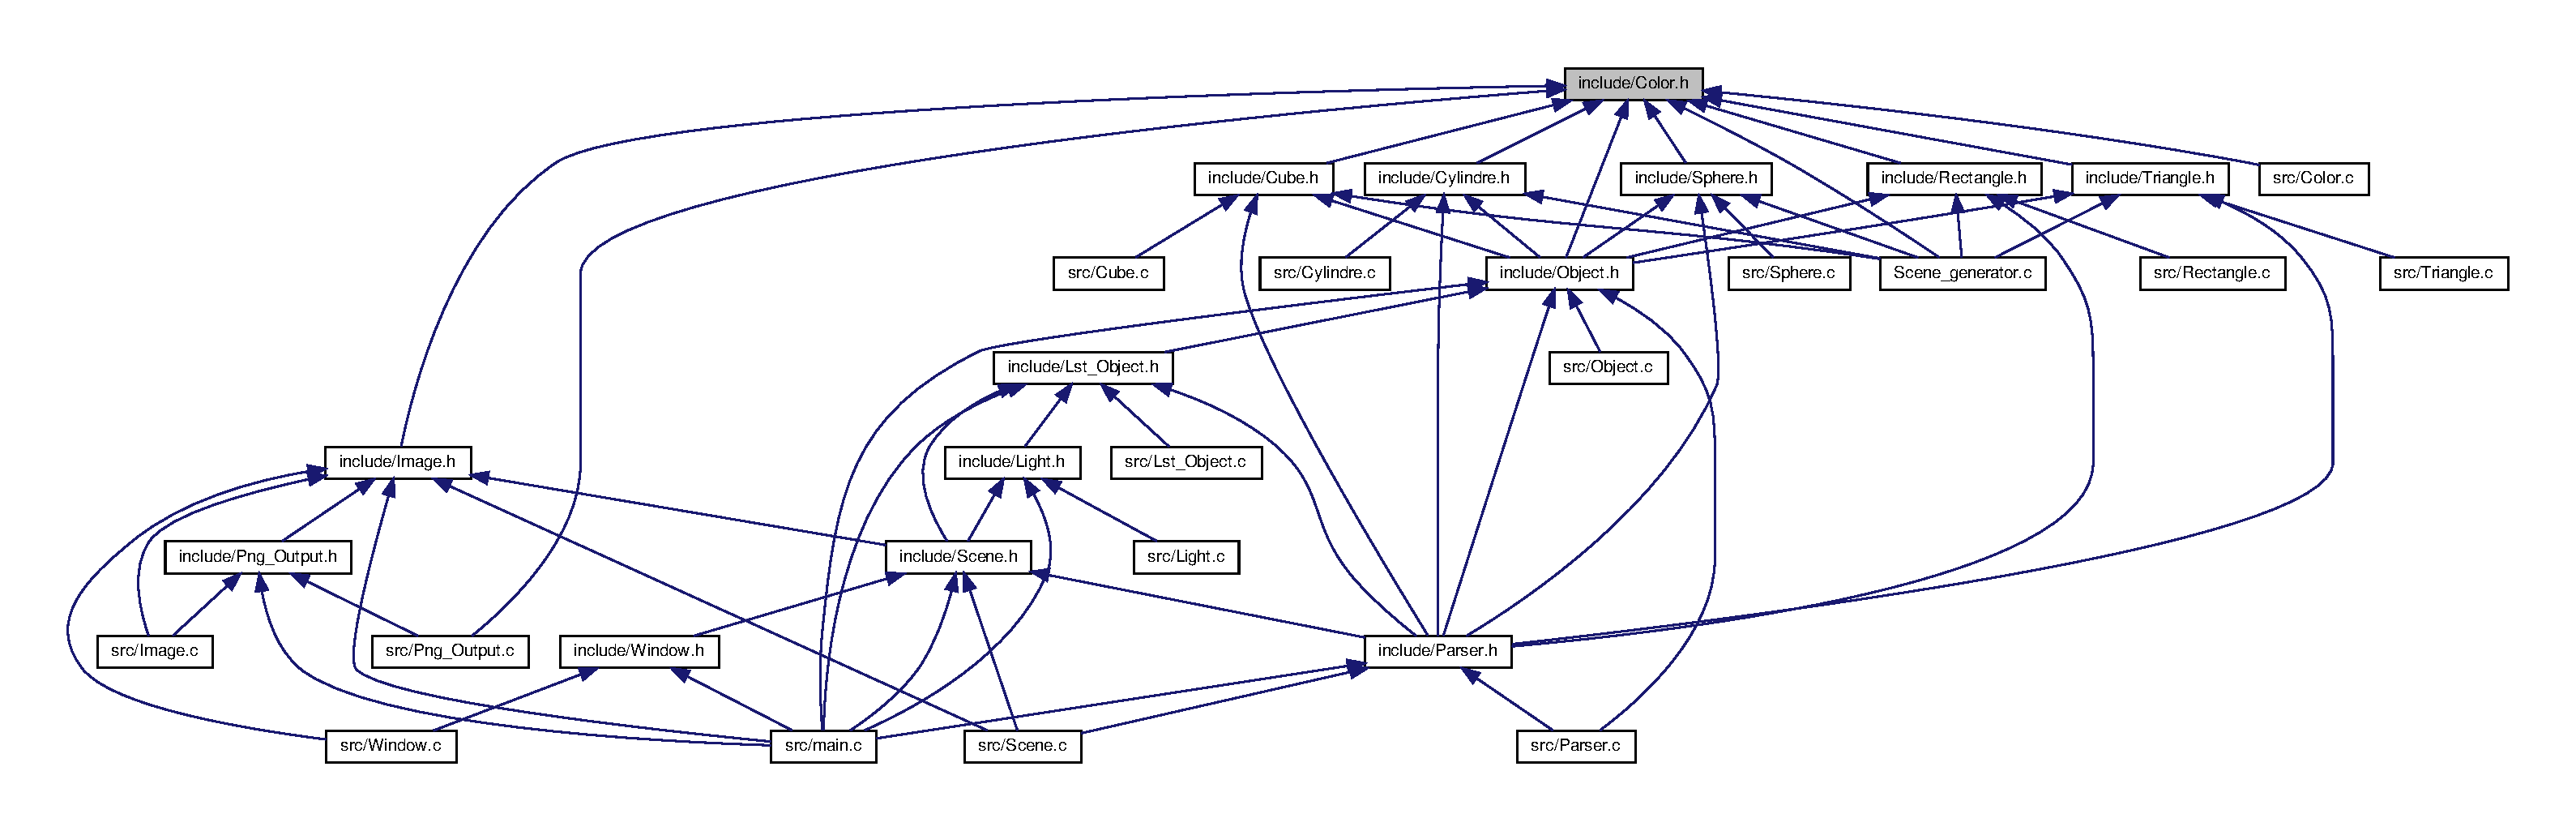
\includegraphics[width=350pt]{_color_8h__dep__incl}
\end{center}
\end{figure}
\subsection*{Data Structures}
\begin{DoxyCompactItemize}
\item 
struct \hyperlink{struct_color}{Color}
\begin{DoxyCompactList}\small\item\em represents R\+GB color \end{DoxyCompactList}\end{DoxyCompactItemize}
\subsection*{Functions}
\begin{DoxyCompactItemize}
\item 
int \hyperlink{_color_8h_aaf343903dcffdb853cb543fb348d72e9}{moyennage\+Color} (int n, const \hyperlink{struct_color}{Color} $\ast$color\+\_\+comming, const \hyperlink{struct_color}{Color} $\ast$color\+\_\+old, \hyperlink{struct_color}{Color} $\ast$res)
\begin{DoxyCompactList}\small\item\em computes a weighted average of two colors \end{DoxyCompactList}\item 
int \hyperlink{_color_8h_af51f46d8c89a637cac181d0234f259fc}{set\+Color} (\hyperlink{struct_color}{Color} $\ast$color, unsigned char r, unsigned char g, unsigned char b)
\begin{DoxyCompactList}\small\item\em sets a color with the specified valuers \end{DoxyCompactList}\item 
int \hyperlink{_color_8h_a54aa1f118af6d46b8ac4902c6f3e2f00}{Color\+Copy} (\hyperlink{struct_color}{Color} $\ast$dest, const \hyperlink{struct_color}{Color} $\ast$src)
\begin{DoxyCompactList}\small\item\em copy a color to another \end{DoxyCompactList}\item 
int \hyperlink{_color_8h_a1f3d5e2bfbaded7521bcd91445516966}{Color\+\_\+to\+\_\+uint32\+\_\+t} (const \hyperlink{struct_color}{Color} $\ast$color, uint32\+\_\+t $\ast$value)
\begin{DoxyCompactList}\small\item\em transform a color to a uint32\+\_\+t value \end{DoxyCompactList}\item 
int \hyperlink{_color_8h_ad44ed96667ce5cc67ae816b097c824de}{Color\+\_\+from\+\_\+double} (\hyperlink{struct_color}{Color} $\ast$color, \hyperlink{g3x__transfo_8h_a89b2b23e407882a535d835574a7912e1}{double} r, \hyperlink{g3x__transfo_8h_a89b2b23e407882a535d835574a7912e1}{double} g, \hyperlink{g3x__transfo_8h_a89b2b23e407882a535d835574a7912e1}{double} b)
\begin{DoxyCompactList}\small\item\em computes R\+GB color from real values \end{DoxyCompactList}\item 
int \hyperlink{_color_8h_ae4fbafaa79776d616aeaf0b8c11e019d}{Color\+Console\+Display} (const \hyperlink{struct_color}{Color} $\ast$c, int return\+\_\+line)
\begin{DoxyCompactList}\small\item\em print a color and all his fiels in console \end{DoxyCompactList}\end{DoxyCompactItemize}


\subsection{Detailed Description}
contains R\+GB color type and all functions related to it 

\begin{DoxyAuthor}{Author}
Jean-\/\+Manuel E\+R\+I\+A\+LC -\/ Hadjer D\+J\+E\+R\+R\+O\+U\+MI 
\end{DoxyAuthor}
\begin{DoxyVersion}{Version}
0.\+1 
\end{DoxyVersion}
\begin{DoxyDate}{Date}
11 juin 2020
\end{DoxyDate}
contains R\+GB color type and all functions related to it 

\subsection{Function Documentation}
\mbox{\Hypertarget{_color_8h_ad44ed96667ce5cc67ae816b097c824de}\label{_color_8h_ad44ed96667ce5cc67ae816b097c824de}} 
\index{Color.\+h@{Color.\+h}!Color\+\_\+from\+\_\+double@{Color\+\_\+from\+\_\+double}}
\index{Color\+\_\+from\+\_\+double@{Color\+\_\+from\+\_\+double}!Color.\+h@{Color.\+h}}
\subsubsection{\texorpdfstring{Color\+\_\+from\+\_\+double()}{Color\_from\_double()}}
{\footnotesize\ttfamily int Color\+\_\+from\+\_\+double (\begin{DoxyParamCaption}\item[{\hyperlink{struct_color}{Color} $\ast$}]{color,  }\item[{\hyperlink{g3x__transfo_8h_a89b2b23e407882a535d835574a7912e1}{double}}]{r,  }\item[{\hyperlink{g3x__transfo_8h_a89b2b23e407882a535d835574a7912e1}{double}}]{g,  }\item[{\hyperlink{g3x__transfo_8h_a89b2b23e407882a535d835574a7912e1}{double}}]{b }\end{DoxyParamCaption})}



computes R\+GB color from real values 


\begin{DoxyParams}{Parameters}
{\em color} & the result color \\
\hline
{\em r} & the red value \\
\hline
{\em g} & the green value \\
\hline
{\em b} & the blue value \\
\hline
\end{DoxyParams}
\begin{DoxyReturn}{Returns}
0 if a error occurs(color == N\+U\+LL)~\newline
 1 otherwise 
\end{DoxyReturn}
\mbox{\Hypertarget{_color_8h_a1f3d5e2bfbaded7521bcd91445516966}\label{_color_8h_a1f3d5e2bfbaded7521bcd91445516966}} 
\index{Color.\+h@{Color.\+h}!Color\+\_\+to\+\_\+uint32\+\_\+t@{Color\+\_\+to\+\_\+uint32\+\_\+t}}
\index{Color\+\_\+to\+\_\+uint32\+\_\+t@{Color\+\_\+to\+\_\+uint32\+\_\+t}!Color.\+h@{Color.\+h}}
\subsubsection{\texorpdfstring{Color\+\_\+to\+\_\+uint32\+\_\+t()}{Color\_to\_uint32\_t()}}
{\footnotesize\ttfamily int Color\+\_\+to\+\_\+uint32\+\_\+t (\begin{DoxyParamCaption}\item[{const \hyperlink{struct_color}{Color} $\ast$}]{color,  }\item[{uint32\+\_\+t $\ast$}]{value }\end{DoxyParamCaption})}



transform a color to a uint32\+\_\+t value 


\begin{DoxyParams}{Parameters}
{\em color} & the color to transform \\
\hline
{\em value} & the result \\
\hline
\end{DoxyParams}
\begin{DoxyReturn}{Returns}
0 if a error occurs(dest == N\+U\+LL $\vert$$\vert$ src == N\+U\+LL)~\newline
 1 otherwise 
\end{DoxyReturn}
\mbox{\Hypertarget{_color_8h_ae4fbafaa79776d616aeaf0b8c11e019d}\label{_color_8h_ae4fbafaa79776d616aeaf0b8c11e019d}} 
\index{Color.\+h@{Color.\+h}!Color\+Console\+Display@{Color\+Console\+Display}}
\index{Color\+Console\+Display@{Color\+Console\+Display}!Color.\+h@{Color.\+h}}
\subsubsection{\texorpdfstring{Color\+Console\+Display()}{ColorConsoleDisplay()}}
{\footnotesize\ttfamily int Color\+Console\+Display (\begin{DoxyParamCaption}\item[{const \hyperlink{struct_color}{Color} $\ast$}]{c,  }\item[{int}]{return\+\_\+line }\end{DoxyParamCaption})}



print a color and all his fiels in console 


\begin{DoxyParams}{Parameters}
{\em c} & the color to print \\
\hline
{\em return\+\_\+line} & if we want to add a \textquotesingle{}~\newline
\textquotesingle{} after the print \\
\hline
\end{DoxyParams}
\mbox{\Hypertarget{_color_8h_a54aa1f118af6d46b8ac4902c6f3e2f00}\label{_color_8h_a54aa1f118af6d46b8ac4902c6f3e2f00}} 
\index{Color.\+h@{Color.\+h}!Color\+Copy@{Color\+Copy}}
\index{Color\+Copy@{Color\+Copy}!Color.\+h@{Color.\+h}}
\subsubsection{\texorpdfstring{Color\+Copy()}{ColorCopy()}}
{\footnotesize\ttfamily int Color\+Copy (\begin{DoxyParamCaption}\item[{\hyperlink{struct_color}{Color} $\ast$}]{dest,  }\item[{const \hyperlink{struct_color}{Color} $\ast$}]{src }\end{DoxyParamCaption})}



copy a color to another 


\begin{DoxyParams}{Parameters}
{\em dest} & the color to change \\
\hline
{\em src} & the copy to copy \\
\hline
\end{DoxyParams}
\begin{DoxyReturn}{Returns}
0 if a error occurs(dest == N\+U\+LL $\vert$$\vert$ src == N\+U\+LL)~\newline
 1 otherwise 
\end{DoxyReturn}
\mbox{\Hypertarget{_color_8h_aaf343903dcffdb853cb543fb348d72e9}\label{_color_8h_aaf343903dcffdb853cb543fb348d72e9}} 
\index{Color.\+h@{Color.\+h}!moyennage\+Color@{moyennage\+Color}}
\index{moyennage\+Color@{moyennage\+Color}!Color.\+h@{Color.\+h}}
\subsubsection{\texorpdfstring{moyennage\+Color()}{moyennageColor()}}
{\footnotesize\ttfamily int moyennage\+Color (\begin{DoxyParamCaption}\item[{int}]{n,  }\item[{const \hyperlink{struct_color}{Color} $\ast$}]{color\+\_\+comming,  }\item[{const \hyperlink{struct_color}{Color} $\ast$}]{color\+\_\+old,  }\item[{\hyperlink{struct_color}{Color} $\ast$}]{res }\end{DoxyParamCaption})}



computes a weighted average of two colors 


\begin{DoxyParams}{Parameters}
{\em n} & the render \\
\hline
{\em color\+\_\+comming} & the first color \\
\hline
{\em color\+\_\+old} & the second color \\
\hline
{\em res} & the result \\
\hline
\end{DoxyParams}
\begin{DoxyReturn}{Returns}
0 if a error occurs(one parameter is N\+U\+L\+L)~\newline
 1 otherwise 
\end{DoxyReturn}
\mbox{\Hypertarget{_color_8h_af51f46d8c89a637cac181d0234f259fc}\label{_color_8h_af51f46d8c89a637cac181d0234f259fc}} 
\index{Color.\+h@{Color.\+h}!set\+Color@{set\+Color}}
\index{set\+Color@{set\+Color}!Color.\+h@{Color.\+h}}
\subsubsection{\texorpdfstring{set\+Color()}{setColor()}}
{\footnotesize\ttfamily int set\+Color (\begin{DoxyParamCaption}\item[{\hyperlink{struct_color}{Color} $\ast$}]{color,  }\item[{unsigned char}]{r,  }\item[{unsigned char}]{g,  }\item[{unsigned char}]{b }\end{DoxyParamCaption})}



sets a color with the specified valuers 


\begin{DoxyParams}{Parameters}
{\em color} & the color to set \\
\hline
{\em r} & the red value \\
\hline
{\em g} & the green value \\
\hline
{\em b} & the blue value \\
\hline
\end{DoxyParams}
\begin{DoxyReturn}{Returns}
0 if a error occurs(color == N\+U\+LL)~\newline
 1 otherwise 
\end{DoxyReturn}

\hypertarget{_cube_8h}{}\section{include/\+Cube.h File Reference}
\label{_cube_8h}\index{include/\+Cube.\+h@{include/\+Cube.\+h}}


contains the \hyperlink{struct_cube}{Cube} type and functions related to it  


{\ttfamily \#include \char`\"{}Color.\+h\char`\"{}}\newline
{\ttfamily \#include \char`\"{}Point.\+h\char`\"{}}\newline
{\ttfamily \#include \char`\"{}Vecteur.\+h\char`\"{}}\newline
Include dependency graph for Cube.\+h\+:\nopagebreak
\begin{figure}[H]
\begin{center}
\leavevmode
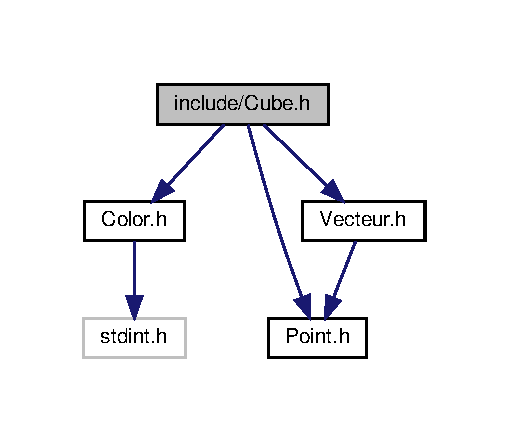
\includegraphics[width=244pt]{_cube_8h__incl}
\end{center}
\end{figure}
This graph shows which files directly or indirectly include this file\+:\nopagebreak
\begin{figure}[H]
\begin{center}
\leavevmode
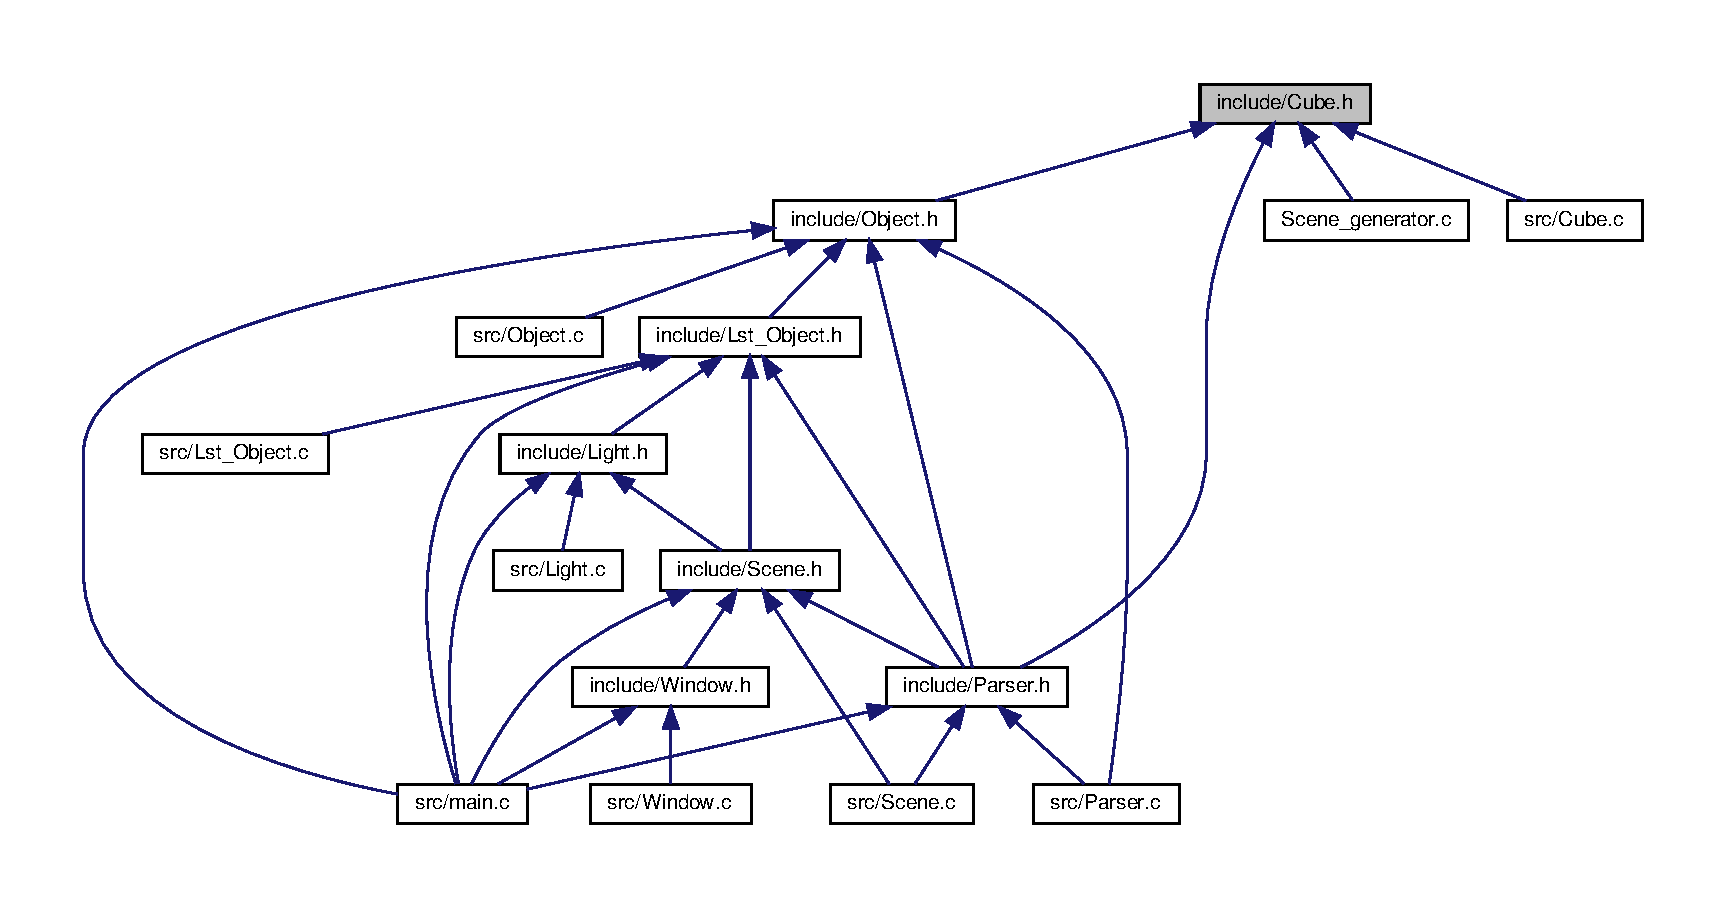
\includegraphics[width=350pt]{_cube_8h__dep__incl}
\end{center}
\end{figure}
\subsection*{Data Structures}
\begin{DoxyCompactItemize}
\item 
struct \hyperlink{struct_cube}{Cube}
\begin{DoxyCompactList}\small\item\em a cube \end{DoxyCompactList}\end{DoxyCompactItemize}
\subsection*{Functions}
\begin{DoxyCompactItemize}
\item 
int \hyperlink{_cube_8h_a06ac4d820420861ff628acafbb739cc2}{set\+Cube} (\hyperlink{struct_cube}{Cube} $\ast$cube, const \hyperlink{struct_point}{Point} $\ast$center, const \hyperlink{struct_color}{Color} $\ast$color, \hyperlink{g3x__transfo_8h_a89b2b23e407882a535d835574a7912e1}{double} rayon)
\begin{DoxyCompactList}\small\item\em sets a cube by the specified parameters \end{DoxyCompactList}\item 
int \hyperlink{_cube_8h_a41a11ebe8d665aa3cf2735e2bb1de084}{rayon\+\_\+inter\+\_\+\+Cube} (const \hyperlink{struct_point}{Point} $\ast$A, const \hyperlink{struct_vecteur}{Vecteur} $\ast$u, \hyperlink{struct_point}{Point} $\ast$I, \hyperlink{struct_vecteur}{Vecteur} $\ast$N)
\begin{DoxyCompactList}\small\item\em check the intersection between a line (A, u) and the canonical cube \end{DoxyCompactList}\item 
int \hyperlink{_cube_8h_abfe9d0a3cc9b3586ef37cc49844e9481}{Cube\+Console\+Display} (const \hyperlink{struct_cube}{Cube} $\ast$cube, int return\+\_\+line)
\begin{DoxyCompactList}\small\item\em print a cube in the console \end{DoxyCompactList}\end{DoxyCompactItemize}


\subsection{Detailed Description}
contains the \hyperlink{struct_cube}{Cube} type and functions related to it 

\begin{DoxyAuthor}{Author}
Jean-\/\+Manuel E\+R\+I\+A\+LC -\/ Hadjer D\+J\+E\+R\+R\+O\+U\+MI 
\end{DoxyAuthor}
\begin{DoxyVersion}{Version}
0.\+1 
\end{DoxyVersion}
\begin{DoxyDate}{Date}
11 juin 2020
\end{DoxyDate}
represents a cube in 3D space and functions related to it 

\subsection{Function Documentation}
\mbox{\Hypertarget{_cube_8h_abfe9d0a3cc9b3586ef37cc49844e9481}\label{_cube_8h_abfe9d0a3cc9b3586ef37cc49844e9481}} 
\index{Cube.\+h@{Cube.\+h}!Cube\+Console\+Display@{Cube\+Console\+Display}}
\index{Cube\+Console\+Display@{Cube\+Console\+Display}!Cube.\+h@{Cube.\+h}}
\subsubsection{\texorpdfstring{Cube\+Console\+Display()}{CubeConsoleDisplay()}}
{\footnotesize\ttfamily int Cube\+Console\+Display (\begin{DoxyParamCaption}\item[{const \hyperlink{struct_cube}{Cube} $\ast$}]{cube,  }\item[{int}]{return\+\_\+line }\end{DoxyParamCaption})}



print a cube in the console 


\begin{DoxyParams}{Parameters}
{\em cube} & the cube to print \\
\hline
{\em return\+\_\+line} & != 0 if we want to add a \textquotesingle{}~\newline
\textquotesingle{} after the print \\
\hline
\end{DoxyParams}
\begin{DoxyReturn}{Returns}
0 if a error occurs(cube == N\+U\+LL)~\newline
 1 otherwise 
\end{DoxyReturn}
\mbox{\Hypertarget{_cube_8h_a41a11ebe8d665aa3cf2735e2bb1de084}\label{_cube_8h_a41a11ebe8d665aa3cf2735e2bb1de084}} 
\index{Cube.\+h@{Cube.\+h}!rayon\+\_\+inter\+\_\+\+Cube@{rayon\+\_\+inter\+\_\+\+Cube}}
\index{rayon\+\_\+inter\+\_\+\+Cube@{rayon\+\_\+inter\+\_\+\+Cube}!Cube.\+h@{Cube.\+h}}
\subsubsection{\texorpdfstring{rayon\+\_\+inter\+\_\+\+Cube()}{rayon\_inter\_Cube()}}
{\footnotesize\ttfamily int rayon\+\_\+inter\+\_\+\+Cube (\begin{DoxyParamCaption}\item[{const \hyperlink{struct_point}{Point} $\ast$}]{A,  }\item[{const \hyperlink{struct_vecteur}{Vecteur} $\ast$}]{u,  }\item[{\hyperlink{struct_point}{Point} $\ast$}]{I,  }\item[{\hyperlink{struct_vecteur}{Vecteur} $\ast$}]{N }\end{DoxyParamCaption})}



check the intersection between a line (A, u) and the canonical cube 


\begin{DoxyParams}{Parameters}
{\em A} & a point of the line \\
\hline
{\em u} & the normalized director vector of the line \\
\hline
{\em I} & the intersection point if it exists \\
\hline
{\em N} & the normal vector in I \\
\hline
\end{DoxyParams}
\begin{DoxyReturn}{Returns}
0 if a error occurs(one parameter is N\+U\+L\+L)~\newline
 1 otherwise 
\end{DoxyReturn}
\mbox{\Hypertarget{_cube_8h_a06ac4d820420861ff628acafbb739cc2}\label{_cube_8h_a06ac4d820420861ff628acafbb739cc2}} 
\index{Cube.\+h@{Cube.\+h}!set\+Cube@{set\+Cube}}
\index{set\+Cube@{set\+Cube}!Cube.\+h@{Cube.\+h}}
\subsubsection{\texorpdfstring{set\+Cube()}{setCube()}}
{\footnotesize\ttfamily int set\+Cube (\begin{DoxyParamCaption}\item[{\hyperlink{struct_cube}{Cube} $\ast$}]{cube,  }\item[{const \hyperlink{struct_point}{Point} $\ast$}]{center,  }\item[{const \hyperlink{struct_color}{Color} $\ast$}]{color,  }\item[{\hyperlink{g3x__transfo_8h_a89b2b23e407882a535d835574a7912e1}{double}}]{rayon }\end{DoxyParamCaption})}



sets a cube by the specified parameters 


\begin{DoxyParams}{Parameters}
{\em cube} & the cube to set \\
\hline
{\em center} & ther new center \\
\hline
{\em color} & the new color \\
\hline
{\em rayon} & the new radius \\
\hline
\end{DoxyParams}
\begin{DoxyReturn}{Returns}
0 if a error occurs(one parameter is N\+U\+L\+L)~\newline
 1 otherwise 
\end{DoxyReturn}

\hypertarget{_cylindre_8h}{}\section{include/\+Cylindre.h File Reference}
\label{_cylindre_8h}\index{include/\+Cylindre.\+h@{include/\+Cylindre.\+h}}


represents a cylinder  


{\ttfamily \#include \char`\"{}Color.\+h\char`\"{}}\newline
{\ttfamily \#include \char`\"{}Point.\+h\char`\"{}}\newline
{\ttfamily \#include \char`\"{}Vecteur.\+h\char`\"{}}\newline
Include dependency graph for Cylindre.\+h\+:\nopagebreak
\begin{figure}[H]
\begin{center}
\leavevmode
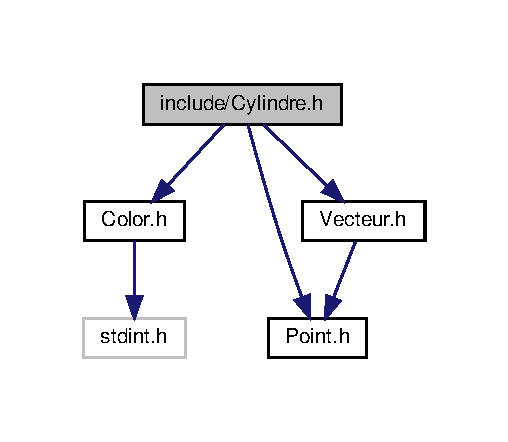
\includegraphics[width=244pt]{_cylindre_8h__incl}
\end{center}
\end{figure}
This graph shows which files directly or indirectly include this file\+:\nopagebreak
\begin{figure}[H]
\begin{center}
\leavevmode
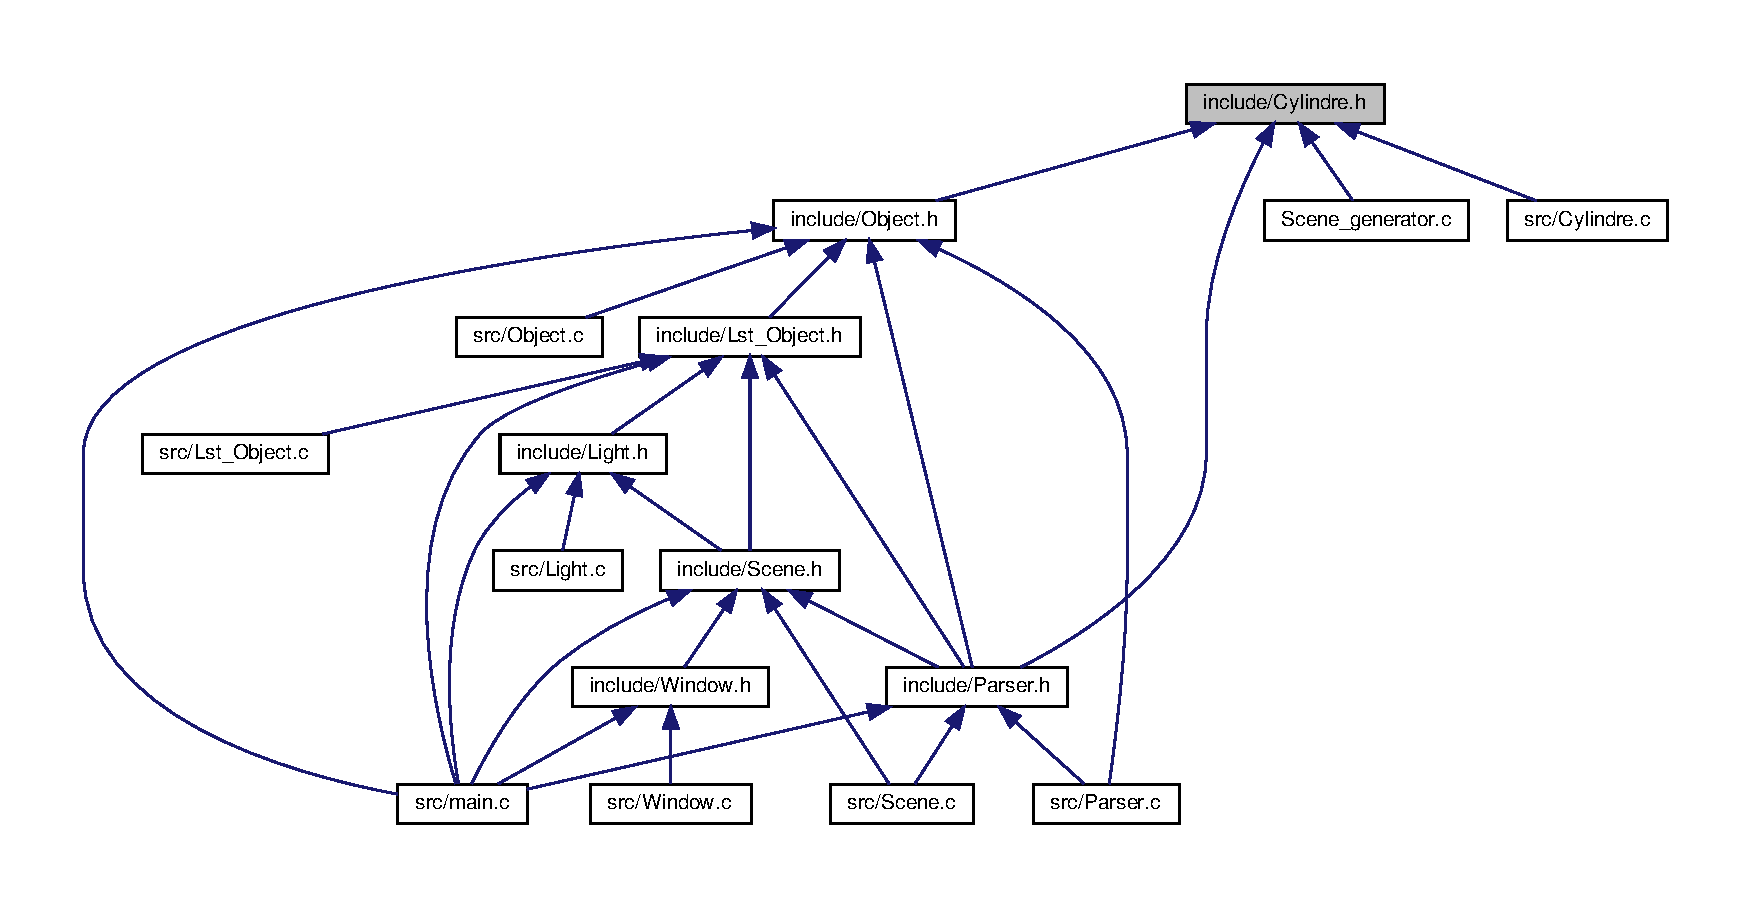
\includegraphics[width=350pt]{_cylindre_8h__dep__incl}
\end{center}
\end{figure}
\subsection*{Data Structures}
\begin{DoxyCompactItemize}
\item 
struct \hyperlink{struct_cylindre}{Cylindre}
\begin{DoxyCompactList}\small\item\em a cylinder \end{DoxyCompactList}\end{DoxyCompactItemize}
\subsection*{Functions}
\begin{DoxyCompactItemize}
\item 
int \hyperlink{_cylindre_8h_ab4c045d8e24bfccc900359db19b116f2}{set\+Cylindre} (\hyperlink{struct_cylindre}{Cylindre} $\ast$cylindre, const \hyperlink{struct_point}{Point} $\ast$P, const \hyperlink{struct_point}{Point} $\ast$Q, const \hyperlink{struct_color}{Color} $\ast$color, \hyperlink{g3x__transfo_8h_a89b2b23e407882a535d835574a7912e1}{double} rayon)
\begin{DoxyCompactList}\small\item\em sets a cylinder with the specified parameters \end{DoxyCompactList}\item 
int \hyperlink{_cylindre_8h_a27b7ad6909df1389d77279245cbbb873}{rayon\+\_\+inter\+\_\+\+Cylindre} (const \hyperlink{struct_point}{Point} $\ast$A, const \hyperlink{struct_vecteur}{Vecteur} $\ast$u, \hyperlink{struct_point}{Point} $\ast$I, \hyperlink{struct_vecteur}{Vecteur} $\ast$N)
\begin{DoxyCompactList}\small\item\em check the intersection between a line (A, u) and the canonical cylinder \end{DoxyCompactList}\item 
int \hyperlink{_cylindre_8h_aef6320ff3a95960aa4c57e149f8d1f55}{rayon\+\_\+inter\+\_\+\+Disque} (const \hyperlink{struct_point}{Point} $\ast$A, const \hyperlink{struct_vecteur}{Vecteur} $\ast$u, \hyperlink{struct_point}{Point} $\ast$I, \hyperlink{struct_vecteur}{Vecteur} $\ast$N, \hyperlink{g3x__transfo_8h_a89b2b23e407882a535d835574a7912e1}{double} d)
\begin{DoxyCompactList}\small\item\em check the intersection between a line (A, u) and the canonical disk in the plane z = d \end{DoxyCompactList}\item 
int \hyperlink{_cylindre_8h_ab0c494740800f14b11f275486cb22e29}{Cylindre\+Console\+Display} (const \hyperlink{struct_cylindre}{Cylindre} $\ast$cylindre, int return\+\_\+line)
\begin{DoxyCompactList}\small\item\em print a cylinder in the console \end{DoxyCompactList}\end{DoxyCompactItemize}


\subsection{Detailed Description}
represents a cylinder 

\begin{DoxyAuthor}{Author}
Jean-\/\+Manuel E\+R\+I\+A\+LC -\/ Hadjer D\+J\+E\+R\+R\+O\+U\+MI 
\end{DoxyAuthor}
\begin{DoxyVersion}{Version}
0.\+1 
\end{DoxyVersion}
\begin{DoxyDate}{Date}
11 juin 2020
\end{DoxyDate}
contains the type representing a cylinder in a 3D space and functions related to it 

\subsection{Function Documentation}
\mbox{\Hypertarget{_cylindre_8h_ab0c494740800f14b11f275486cb22e29}\label{_cylindre_8h_ab0c494740800f14b11f275486cb22e29}} 
\index{Cylindre.\+h@{Cylindre.\+h}!Cylindre\+Console\+Display@{Cylindre\+Console\+Display}}
\index{Cylindre\+Console\+Display@{Cylindre\+Console\+Display}!Cylindre.\+h@{Cylindre.\+h}}
\subsubsection{\texorpdfstring{Cylindre\+Console\+Display()}{CylindreConsoleDisplay()}}
{\footnotesize\ttfamily int Cylindre\+Console\+Display (\begin{DoxyParamCaption}\item[{const \hyperlink{struct_cylindre}{Cylindre} $\ast$}]{cylindre,  }\item[{int}]{return\+\_\+line }\end{DoxyParamCaption})}



print a cylinder in the console 


\begin{DoxyParams}{Parameters}
{\em cylindre} & the cylinder to print \\
\hline
{\em return\+\_\+line} & != 0 if we want to add a \textquotesingle{}~\newline
\textquotesingle{} after the print \\
\hline
\end{DoxyParams}
\begin{DoxyReturn}{Returns}
0 if a error occurs(cylinder == N\+U\+LL)~\newline
 1 otherwise 
\end{DoxyReturn}
\mbox{\Hypertarget{_cylindre_8h_a27b7ad6909df1389d77279245cbbb873}\label{_cylindre_8h_a27b7ad6909df1389d77279245cbbb873}} 
\index{Cylindre.\+h@{Cylindre.\+h}!rayon\+\_\+inter\+\_\+\+Cylindre@{rayon\+\_\+inter\+\_\+\+Cylindre}}
\index{rayon\+\_\+inter\+\_\+\+Cylindre@{rayon\+\_\+inter\+\_\+\+Cylindre}!Cylindre.\+h@{Cylindre.\+h}}
\subsubsection{\texorpdfstring{rayon\+\_\+inter\+\_\+\+Cylindre()}{rayon\_inter\_Cylindre()}}
{\footnotesize\ttfamily int rayon\+\_\+inter\+\_\+\+Cylindre (\begin{DoxyParamCaption}\item[{const \hyperlink{struct_point}{Point} $\ast$}]{A,  }\item[{const \hyperlink{struct_vecteur}{Vecteur} $\ast$}]{u,  }\item[{\hyperlink{struct_point}{Point} $\ast$}]{I,  }\item[{\hyperlink{struct_vecteur}{Vecteur} $\ast$}]{N }\end{DoxyParamCaption})}



check the intersection between a line (A, u) and the canonical cylinder 


\begin{DoxyParams}{Parameters}
{\em A} & a point of the line \\
\hline
{\em u} & the normalized director vector of the line \\
\hline
{\em I} & the intersection point if it exists \\
\hline
{\em N} & the normal vector in I \\
\hline
\end{DoxyParams}
\begin{DoxyReturn}{Returns}
0 if a error occurs(one parameter is N\+U\+L\+L)~\newline
 1 otherwise 
\end{DoxyReturn}
\mbox{\Hypertarget{_cylindre_8h_aef6320ff3a95960aa4c57e149f8d1f55}\label{_cylindre_8h_aef6320ff3a95960aa4c57e149f8d1f55}} 
\index{Cylindre.\+h@{Cylindre.\+h}!rayon\+\_\+inter\+\_\+\+Disque@{rayon\+\_\+inter\+\_\+\+Disque}}
\index{rayon\+\_\+inter\+\_\+\+Disque@{rayon\+\_\+inter\+\_\+\+Disque}!Cylindre.\+h@{Cylindre.\+h}}
\subsubsection{\texorpdfstring{rayon\+\_\+inter\+\_\+\+Disque()}{rayon\_inter\_Disque()}}
{\footnotesize\ttfamily int rayon\+\_\+inter\+\_\+\+Disque (\begin{DoxyParamCaption}\item[{const \hyperlink{struct_point}{Point} $\ast$}]{A,  }\item[{const \hyperlink{struct_vecteur}{Vecteur} $\ast$}]{u,  }\item[{\hyperlink{struct_point}{Point} $\ast$}]{I,  }\item[{\hyperlink{struct_vecteur}{Vecteur} $\ast$}]{N,  }\item[{\hyperlink{g3x__transfo_8h_a89b2b23e407882a535d835574a7912e1}{double}}]{d }\end{DoxyParamCaption})}



check the intersection between a line (A, u) and the canonical disk in the plane z = d 


\begin{DoxyParams}{Parameters}
{\em A} & a point of the line \\
\hline
{\em u} & the normalized director vector of the line \\
\hline
{\em I} & the intersection point if it exists \\
\hline
{\em N} & the normal vector in I \\
\hline
{\em d} & the d in the plane equation z = d \\
\hline
\end{DoxyParams}
\begin{DoxyReturn}{Returns}
0 if a error occurs(one parameter is N\+U\+L\+L)~\newline
 1 otherwise 
\end{DoxyReturn}
\mbox{\Hypertarget{_cylindre_8h_ab4c045d8e24bfccc900359db19b116f2}\label{_cylindre_8h_ab4c045d8e24bfccc900359db19b116f2}} 
\index{Cylindre.\+h@{Cylindre.\+h}!set\+Cylindre@{set\+Cylindre}}
\index{set\+Cylindre@{set\+Cylindre}!Cylindre.\+h@{Cylindre.\+h}}
\subsubsection{\texorpdfstring{set\+Cylindre()}{setCylindre()}}
{\footnotesize\ttfamily int set\+Cylindre (\begin{DoxyParamCaption}\item[{\hyperlink{struct_cylindre}{Cylindre} $\ast$}]{cylindre,  }\item[{const \hyperlink{struct_point}{Point} $\ast$}]{P,  }\item[{const \hyperlink{struct_point}{Point} $\ast$}]{Q,  }\item[{const \hyperlink{struct_color}{Color} $\ast$}]{color,  }\item[{\hyperlink{g3x__transfo_8h_a89b2b23e407882a535d835574a7912e1}{double}}]{rayon }\end{DoxyParamCaption})}



sets a cylinder with the specified parameters 


\begin{DoxyParams}{Parameters}
{\em cylindre} & the cylinder to set \\
\hline
{\em P} & the new first point \\
\hline
{\em Q} & the new second point \\
\hline
{\em color} & the new color \\
\hline
{\em rayon} & the new radius \\
\hline
\end{DoxyParams}
\begin{DoxyReturn}{Returns}
0 if a error occurs(one parameter is N\+U\+L\+L)~\newline
 1 otherwise 
\end{DoxyReturn}

\hypertarget{_hmat_8h}{}\section{include/\+Hmat.h File Reference}
\label{_hmat_8h}\index{include/\+Hmat.\+h@{include/\+Hmat.\+h}}


contains the type Hmat representing homogeneous matrices and functions related to if  


{\ttfamily \#include \char`\"{}Vecteur.\+h\char`\"{}}\newline
Include dependency graph for Hmat.\+h\+:\nopagebreak
\begin{figure}[H]
\begin{center}
\leavevmode
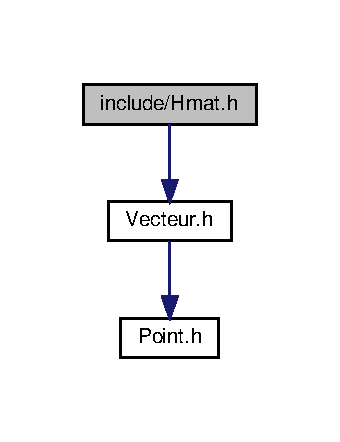
\includegraphics[width=163pt]{_hmat_8h__incl}
\end{center}
\end{figure}
This graph shows which files directly or indirectly include this file\+:\nopagebreak
\begin{figure}[H]
\begin{center}
\leavevmode
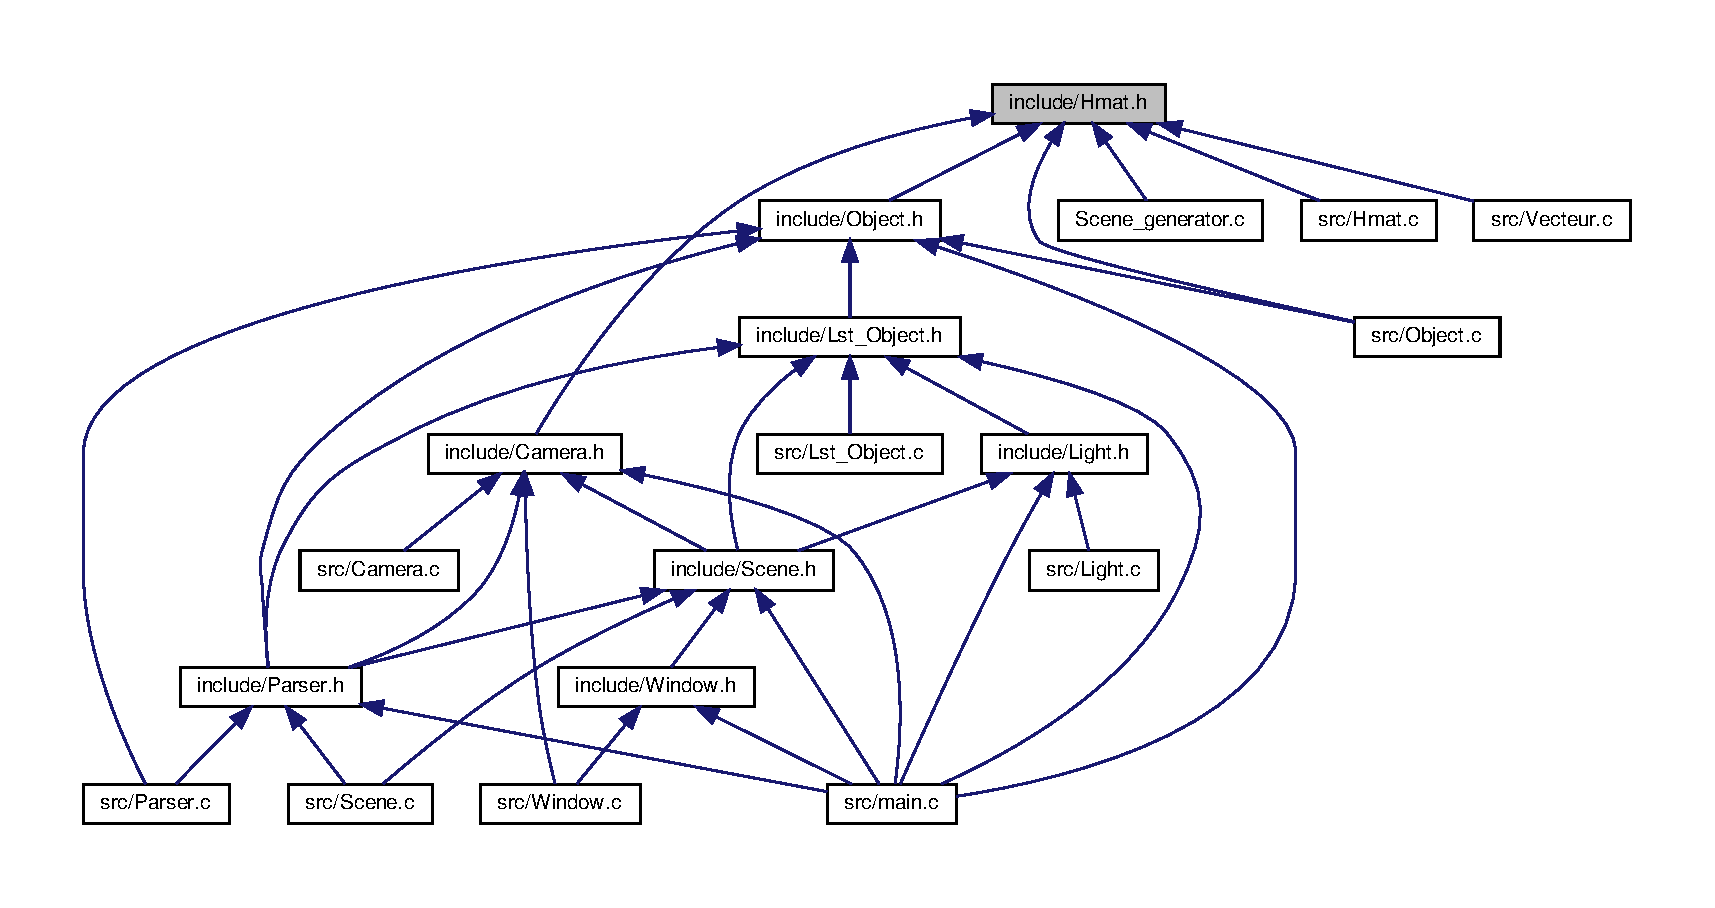
\includegraphics[width=350pt]{_hmat_8h__dep__incl}
\end{center}
\end{figure}
\subsection*{Macros}
\begin{DoxyCompactItemize}
\item 
\#define \hyperlink{_hmat_8h_a29ab8f304572bfb421e3f7666da0fe4d}{A00}~0
\item 
\#define \hyperlink{_hmat_8h_a105b3dbbda7ff665ef1369a7ea42f29d}{A01}~1
\item 
\#define \hyperlink{_hmat_8h_a5663784dabb95a65df02aa05f514f61a}{A02}~2
\item 
\#define \hyperlink{_hmat_8h_a9120b75c74b7b27376f81d53287bf02d}{A03}~3
\item 
\#define \hyperlink{_hmat_8h_aa9c8a71816927936216695bafcec4a75}{A10}~4
\item 
\#define \hyperlink{_hmat_8h_aa8394a82104d1917c30c5e017ccf6176}{A11}~5
\item 
\#define \hyperlink{_hmat_8h_a84e5fa24b6bb47717a091f89de79b601}{A12}~6
\item 
\#define \hyperlink{_hmat_8h_a23c0012e8b708484ade6b708b4fad480}{A13}~7
\item 
\#define \hyperlink{_hmat_8h_a0f72c217c2cac6efbfe84fbb41afb298}{A20}~8
\item 
\#define \hyperlink{_hmat_8h_aa464bb5d73d5326f59cfe1e6d2b38a2b}{A21}~9
\item 
\#define \hyperlink{_hmat_8h_a69da8b81ea4b9ca7dd631a4320794884}{A22}~10
\item 
\#define \hyperlink{_hmat_8h_a1acc33cef8fdaaef9f2268ad573c0414}{A23}~11
\item 
\#define \hyperlink{_hmat_8h_a7945469a2ffa989fec01b0aa3511aa10}{A30}~12
\item 
\#define \hyperlink{_hmat_8h_ab7b4194499b52e3137ff31393e307d2b}{A31}~13
\item 
\#define \hyperlink{_hmat_8h_ab261da7f384997d46b5fa366592be481}{A32}~14
\item 
\#define \hyperlink{_hmat_8h_ac57896e0467dfc90495d64e7b05169c1}{A33}~15
\item 
\#define \hyperlink{_hmat_8h_acba9dc9ee1dad7e646bd51297a284abb}{Hmat\+\_\+\+S\+I\+ZE}~16
\item 
\#define \hyperlink{_hmat_8h_aac74276a3384b1fcae5ee7d98aa8ecb6}{Hmat\+\_\+\+E\+L\+E\+M\+E\+N\+T\+\_\+\+P\+E\+R\+\_\+\+L\+I\+NE}~4
\end{DoxyCompactItemize}
\subsection*{Typedefs}
\begin{DoxyCompactItemize}
\item 
typedef \hyperlink{g3x__transfo_8h_a89b2b23e407882a535d835574a7912e1}{double} \hyperlink{_hmat_8h_a7263a9d077d77f58425e01446b766c9f}{Hmat}\mbox{[}\hyperlink{_hmat_8h_acba9dc9ee1dad7e646bd51297a284abb}{Hmat\+\_\+\+S\+I\+ZE}\mbox{]}
\end{DoxyCompactItemize}
\subsection*{Functions}
\begin{DoxyCompactItemize}
\item 
int \hyperlink{_hmat_8h_a10e448c738a6abf525bc835ff72566c6}{Hmat\+Identity} (\hyperlink{_hmat_8h_a7263a9d077d77f58425e01446b766c9f}{Hmat} mat)
\begin{DoxyCompactList}\small\item\em create and initialize a matrix with identity \end{DoxyCompactList}\item 
int \hyperlink{_hmat_8h_a5c6553d5c66956733c3f3d7c9c6f8312}{Hmat\+\_\+fill\+\_\+with\+\_\+value} (\hyperlink{_hmat_8h_a7263a9d077d77f58425e01446b766c9f}{Hmat} mat, \hyperlink{g3x__transfo_8h_a89b2b23e407882a535d835574a7912e1}{double} value)
\begin{DoxyCompactList}\small\item\em assign the given value to all elements of the given matrix \end{DoxyCompactList}\item 
int \hyperlink{_hmat_8h_acfea46fe40d40ab0a0cc0454ced9c362}{Hmat\+\_\+get\+\_\+value} (const \hyperlink{_hmat_8h_a7263a9d077d77f58425e01446b766c9f}{Hmat} mat, int i, int j, \hyperlink{g3x__transfo_8h_a89b2b23e407882a535d835574a7912e1}{double} $\ast$res)
\begin{DoxyCompactList}\small\item\em get the value in the specified position of a given matrix \end{DoxyCompactList}\item 
int \hyperlink{_hmat_8h_a2464ba0c7398a49caaae038cb6bbecf0}{Hmat\+\_\+set\+\_\+value} (\hyperlink{_hmat_8h_a7263a9d077d77f58425e01446b766c9f}{Hmat} mat, int i, int j, \hyperlink{g3x__transfo_8h_a89b2b23e407882a535d835574a7912e1}{double} value)
\begin{DoxyCompactList}\small\item\em set the value in the specified position of a given matrix \end{DoxyCompactList}\item 
int \hyperlink{_hmat_8h_af11a77803a87f14bb14e00b154b43750}{Hmat\+\_\+translation\+\_\+\+Vecteur} (\hyperlink{_hmat_8h_a7263a9d077d77f58425e01446b766c9f}{Hmat} mat, const \hyperlink{struct_vecteur}{Vecteur} $\ast$v)
\begin{DoxyCompactList}\small\item\em create the translation matrix corresponding to a vector v \end{DoxyCompactList}\item 
int \hyperlink{_hmat_8h_a7002d0e43f989d847d4c575638bc2547}{Hmat\+\_\+translation\+\_\+\+Hmatxyz} (\hyperlink{_hmat_8h_a7263a9d077d77f58425e01446b766c9f}{Hmat} mat, \hyperlink{g3x__transfo_8h_a89b2b23e407882a535d835574a7912e1}{double} x, \hyperlink{g3x__transfo_8h_a89b2b23e407882a535d835574a7912e1}{double} y, \hyperlink{g3x__transfo_8h_a89b2b23e407882a535d835574a7912e1}{double} z)
\begin{DoxyCompactList}\small\item\em create the translation matrix corresponding to the given values \end{DoxyCompactList}\item 
int \hyperlink{_hmat_8h_ac980a5406219724b6c990e737163b210}{Hmat\+\_\+x\+\_\+\+Point} (const \hyperlink{_hmat_8h_a7263a9d077d77f58425e01446b766c9f}{Hmat} mat, const \hyperlink{struct_point}{Point} $\ast$p, \hyperlink{struct_point}{Point} $\ast$res)
\begin{DoxyCompactList}\small\item\em transform the given point with the given homogeneous matrix \end{DoxyCompactList}\item 
int \hyperlink{_hmat_8h_a93062d33d860d348ec8d85bf26d0fff3}{Hmat\+\_\+x\+\_\+\+Vecteur} (const \hyperlink{_hmat_8h_a7263a9d077d77f58425e01446b766c9f}{Hmat} mat, const \hyperlink{struct_vecteur}{Vecteur} $\ast$vec, \hyperlink{struct_vecteur}{Vecteur} $\ast$res)
\begin{DoxyCompactList}\small\item\em transform the given vector with the given homogeneous matrix \end{DoxyCompactList}\item 
int \hyperlink{_hmat_8h_adece7d8d83ea85f25a33c9857f852bbc}{Hmat\+\_\+x\+\_\+\+Vec} (const \hyperlink{_hmat_8h_a7263a9d077d77f58425e01446b766c9f}{Hmat} mat, \hyperlink{struct_vecteur}{Vecteur} $\ast$vec)
\begin{DoxyCompactList}\small\item\em transform the given vector with the given homogeneous matrix \end{DoxyCompactList}\item 
int \hyperlink{_hmat_8h_ae6488381ad30432c19bbed5c6293b066}{Hmat\+\_\+x\+\_\+\+Hmat} (const \hyperlink{_hmat_8h_a7263a9d077d77f58425e01446b766c9f}{Hmat} A, const \hyperlink{_hmat_8h_a7263a9d077d77f58425e01446b766c9f}{Hmat} B, \hyperlink{_hmat_8h_a7263a9d077d77f58425e01446b766c9f}{Hmat} res)
\begin{DoxyCompactList}\small\item\em matrix product \end{DoxyCompactList}\item 
int \hyperlink{_hmat_8h_ae58098a9e5066da52de171ee1bc9bd61}{Homothetie} (\hyperlink{_hmat_8h_a7263a9d077d77f58425e01446b766c9f}{Hmat} res, \hyperlink{g3x__transfo_8h_a89b2b23e407882a535d835574a7912e1}{double} a, \hyperlink{g3x__transfo_8h_a89b2b23e407882a535d835574a7912e1}{double} b, \hyperlink{g3x__transfo_8h_a89b2b23e407882a535d835574a7912e1}{double} c)
\begin{DoxyCompactList}\small\item\em create the homothety matrix corresponding to the given parameters \end{DoxyCompactList}\item 
void \hyperlink{_hmat_8h_a0ae1ebe5a199bceabe73104771bf5239}{Hmat\+Display} (\hyperlink{_hmat_8h_a7263a9d077d77f58425e01446b766c9f}{Hmat} mat)
\begin{DoxyCompactList}\small\item\em print a matrix in the console \end{DoxyCompactList}\end{DoxyCompactItemize}


\subsection{Detailed Description}
contains the type Hmat representing homogeneous matrices and functions related to if 

\begin{DoxyAuthor}{Author}
Jean-\/\+Manuel E\+R\+I\+A\+LC -\/ Hadjer D\+J\+E\+R\+R\+O\+U\+MI 
\end{DoxyAuthor}
\begin{DoxyVersion}{Version}
0.\+1 
\end{DoxyVersion}
\begin{DoxyDate}{Date}
11 juin 2020
\end{DoxyDate}
contains the type Hmat representing homogeneous matrices and functions related to this type witch are used to transform objects in the 3D space 

\subsection{Macro Definition Documentation}
\mbox{\Hypertarget{_hmat_8h_a29ab8f304572bfb421e3f7666da0fe4d}\label{_hmat_8h_a29ab8f304572bfb421e3f7666da0fe4d}} 
\index{Hmat.\+h@{Hmat.\+h}!A00@{A00}}
\index{A00@{A00}!Hmat.\+h@{Hmat.\+h}}
\subsubsection{\texorpdfstring{A00}{A00}}
{\footnotesize\ttfamily \#define A00~0}

\mbox{\Hypertarget{_hmat_8h_a105b3dbbda7ff665ef1369a7ea42f29d}\label{_hmat_8h_a105b3dbbda7ff665ef1369a7ea42f29d}} 
\index{Hmat.\+h@{Hmat.\+h}!A01@{A01}}
\index{A01@{A01}!Hmat.\+h@{Hmat.\+h}}
\subsubsection{\texorpdfstring{A01}{A01}}
{\footnotesize\ttfamily \#define A01~1}

\mbox{\Hypertarget{_hmat_8h_a5663784dabb95a65df02aa05f514f61a}\label{_hmat_8h_a5663784dabb95a65df02aa05f514f61a}} 
\index{Hmat.\+h@{Hmat.\+h}!A02@{A02}}
\index{A02@{A02}!Hmat.\+h@{Hmat.\+h}}
\subsubsection{\texorpdfstring{A02}{A02}}
{\footnotesize\ttfamily \#define A02~2}

\mbox{\Hypertarget{_hmat_8h_a9120b75c74b7b27376f81d53287bf02d}\label{_hmat_8h_a9120b75c74b7b27376f81d53287bf02d}} 
\index{Hmat.\+h@{Hmat.\+h}!A03@{A03}}
\index{A03@{A03}!Hmat.\+h@{Hmat.\+h}}
\subsubsection{\texorpdfstring{A03}{A03}}
{\footnotesize\ttfamily \#define A03~3}

\mbox{\Hypertarget{_hmat_8h_aa9c8a71816927936216695bafcec4a75}\label{_hmat_8h_aa9c8a71816927936216695bafcec4a75}} 
\index{Hmat.\+h@{Hmat.\+h}!A10@{A10}}
\index{A10@{A10}!Hmat.\+h@{Hmat.\+h}}
\subsubsection{\texorpdfstring{A10}{A10}}
{\footnotesize\ttfamily \#define A10~4}

\mbox{\Hypertarget{_hmat_8h_aa8394a82104d1917c30c5e017ccf6176}\label{_hmat_8h_aa8394a82104d1917c30c5e017ccf6176}} 
\index{Hmat.\+h@{Hmat.\+h}!A11@{A11}}
\index{A11@{A11}!Hmat.\+h@{Hmat.\+h}}
\subsubsection{\texorpdfstring{A11}{A11}}
{\footnotesize\ttfamily \#define A11~5}

\mbox{\Hypertarget{_hmat_8h_a84e5fa24b6bb47717a091f89de79b601}\label{_hmat_8h_a84e5fa24b6bb47717a091f89de79b601}} 
\index{Hmat.\+h@{Hmat.\+h}!A12@{A12}}
\index{A12@{A12}!Hmat.\+h@{Hmat.\+h}}
\subsubsection{\texorpdfstring{A12}{A12}}
{\footnotesize\ttfamily \#define A12~6}

\mbox{\Hypertarget{_hmat_8h_a23c0012e8b708484ade6b708b4fad480}\label{_hmat_8h_a23c0012e8b708484ade6b708b4fad480}} 
\index{Hmat.\+h@{Hmat.\+h}!A13@{A13}}
\index{A13@{A13}!Hmat.\+h@{Hmat.\+h}}
\subsubsection{\texorpdfstring{A13}{A13}}
{\footnotesize\ttfamily \#define A13~7}

\mbox{\Hypertarget{_hmat_8h_a0f72c217c2cac6efbfe84fbb41afb298}\label{_hmat_8h_a0f72c217c2cac6efbfe84fbb41afb298}} 
\index{Hmat.\+h@{Hmat.\+h}!A20@{A20}}
\index{A20@{A20}!Hmat.\+h@{Hmat.\+h}}
\subsubsection{\texorpdfstring{A20}{A20}}
{\footnotesize\ttfamily \#define A20~8}

\mbox{\Hypertarget{_hmat_8h_aa464bb5d73d5326f59cfe1e6d2b38a2b}\label{_hmat_8h_aa464bb5d73d5326f59cfe1e6d2b38a2b}} 
\index{Hmat.\+h@{Hmat.\+h}!A21@{A21}}
\index{A21@{A21}!Hmat.\+h@{Hmat.\+h}}
\subsubsection{\texorpdfstring{A21}{A21}}
{\footnotesize\ttfamily \#define A21~9}

\mbox{\Hypertarget{_hmat_8h_a69da8b81ea4b9ca7dd631a4320794884}\label{_hmat_8h_a69da8b81ea4b9ca7dd631a4320794884}} 
\index{Hmat.\+h@{Hmat.\+h}!A22@{A22}}
\index{A22@{A22}!Hmat.\+h@{Hmat.\+h}}
\subsubsection{\texorpdfstring{A22}{A22}}
{\footnotesize\ttfamily \#define A22~10}

\mbox{\Hypertarget{_hmat_8h_a1acc33cef8fdaaef9f2268ad573c0414}\label{_hmat_8h_a1acc33cef8fdaaef9f2268ad573c0414}} 
\index{Hmat.\+h@{Hmat.\+h}!A23@{A23}}
\index{A23@{A23}!Hmat.\+h@{Hmat.\+h}}
\subsubsection{\texorpdfstring{A23}{A23}}
{\footnotesize\ttfamily \#define A23~11}

\mbox{\Hypertarget{_hmat_8h_a7945469a2ffa989fec01b0aa3511aa10}\label{_hmat_8h_a7945469a2ffa989fec01b0aa3511aa10}} 
\index{Hmat.\+h@{Hmat.\+h}!A30@{A30}}
\index{A30@{A30}!Hmat.\+h@{Hmat.\+h}}
\subsubsection{\texorpdfstring{A30}{A30}}
{\footnotesize\ttfamily \#define A30~12}

\mbox{\Hypertarget{_hmat_8h_ab7b4194499b52e3137ff31393e307d2b}\label{_hmat_8h_ab7b4194499b52e3137ff31393e307d2b}} 
\index{Hmat.\+h@{Hmat.\+h}!A31@{A31}}
\index{A31@{A31}!Hmat.\+h@{Hmat.\+h}}
\subsubsection{\texorpdfstring{A31}{A31}}
{\footnotesize\ttfamily \#define A31~13}

\mbox{\Hypertarget{_hmat_8h_ab261da7f384997d46b5fa366592be481}\label{_hmat_8h_ab261da7f384997d46b5fa366592be481}} 
\index{Hmat.\+h@{Hmat.\+h}!A32@{A32}}
\index{A32@{A32}!Hmat.\+h@{Hmat.\+h}}
\subsubsection{\texorpdfstring{A32}{A32}}
{\footnotesize\ttfamily \#define A32~14}

\mbox{\Hypertarget{_hmat_8h_ac57896e0467dfc90495d64e7b05169c1}\label{_hmat_8h_ac57896e0467dfc90495d64e7b05169c1}} 
\index{Hmat.\+h@{Hmat.\+h}!A33@{A33}}
\index{A33@{A33}!Hmat.\+h@{Hmat.\+h}}
\subsubsection{\texorpdfstring{A33}{A33}}
{\footnotesize\ttfamily \#define A33~15}

\mbox{\Hypertarget{_hmat_8h_aac74276a3384b1fcae5ee7d98aa8ecb6}\label{_hmat_8h_aac74276a3384b1fcae5ee7d98aa8ecb6}} 
\index{Hmat.\+h@{Hmat.\+h}!Hmat\+\_\+\+E\+L\+E\+M\+E\+N\+T\+\_\+\+P\+E\+R\+\_\+\+L\+I\+NE@{Hmat\+\_\+\+E\+L\+E\+M\+E\+N\+T\+\_\+\+P\+E\+R\+\_\+\+L\+I\+NE}}
\index{Hmat\+\_\+\+E\+L\+E\+M\+E\+N\+T\+\_\+\+P\+E\+R\+\_\+\+L\+I\+NE@{Hmat\+\_\+\+E\+L\+E\+M\+E\+N\+T\+\_\+\+P\+E\+R\+\_\+\+L\+I\+NE}!Hmat.\+h@{Hmat.\+h}}
\subsubsection{\texorpdfstring{Hmat\+\_\+\+E\+L\+E\+M\+E\+N\+T\+\_\+\+P\+E\+R\+\_\+\+L\+I\+NE}{Hmat\_ELEMENT\_PER\_LINE}}
{\footnotesize\ttfamily \#define Hmat\+\_\+\+E\+L\+E\+M\+E\+N\+T\+\_\+\+P\+E\+R\+\_\+\+L\+I\+NE~4}

\mbox{\Hypertarget{_hmat_8h_acba9dc9ee1dad7e646bd51297a284abb}\label{_hmat_8h_acba9dc9ee1dad7e646bd51297a284abb}} 
\index{Hmat.\+h@{Hmat.\+h}!Hmat\+\_\+\+S\+I\+ZE@{Hmat\+\_\+\+S\+I\+ZE}}
\index{Hmat\+\_\+\+S\+I\+ZE@{Hmat\+\_\+\+S\+I\+ZE}!Hmat.\+h@{Hmat.\+h}}
\subsubsection{\texorpdfstring{Hmat\+\_\+\+S\+I\+ZE}{Hmat\_SIZE}}
{\footnotesize\ttfamily \#define Hmat\+\_\+\+S\+I\+ZE~16}



\subsection{Typedef Documentation}
\mbox{\Hypertarget{_hmat_8h_a7263a9d077d77f58425e01446b766c9f}\label{_hmat_8h_a7263a9d077d77f58425e01446b766c9f}} 
\index{Hmat.\+h@{Hmat.\+h}!Hmat@{Hmat}}
\index{Hmat@{Hmat}!Hmat.\+h@{Hmat.\+h}}
\subsubsection{\texorpdfstring{Hmat}{Hmat}}
{\footnotesize\ttfamily typedef \hyperlink{g3x__transfo_8h_a89b2b23e407882a535d835574a7912e1}{double} Hmat\mbox{[}\hyperlink{_hmat_8h_acba9dc9ee1dad7e646bd51297a284abb}{Hmat\+\_\+\+S\+I\+ZE}\mbox{]}}

the Hmat type is an array of size Hmat\+\_\+\+S\+I\+ZE witch represents a 4 x 4 matrix 

\subsection{Function Documentation}
\mbox{\Hypertarget{_hmat_8h_a5c6553d5c66956733c3f3d7c9c6f8312}\label{_hmat_8h_a5c6553d5c66956733c3f3d7c9c6f8312}} 
\index{Hmat.\+h@{Hmat.\+h}!Hmat\+\_\+fill\+\_\+with\+\_\+value@{Hmat\+\_\+fill\+\_\+with\+\_\+value}}
\index{Hmat\+\_\+fill\+\_\+with\+\_\+value@{Hmat\+\_\+fill\+\_\+with\+\_\+value}!Hmat.\+h@{Hmat.\+h}}
\subsubsection{\texorpdfstring{Hmat\+\_\+fill\+\_\+with\+\_\+value()}{Hmat\_fill\_with\_value()}}
{\footnotesize\ttfamily int Hmat\+\_\+fill\+\_\+with\+\_\+value (\begin{DoxyParamCaption}\item[{\hyperlink{_hmat_8h_a7263a9d077d77f58425e01446b766c9f}{Hmat}}]{mat,  }\item[{\hyperlink{g3x__transfo_8h_a89b2b23e407882a535d835574a7912e1}{double}}]{value }\end{DoxyParamCaption})}



assign the given value to all elements of the given matrix 


\begin{DoxyParams}{Parameters}
{\em mat} & the given matrix \\
\hline
{\em value} & the given value \\
\hline
\end{DoxyParams}
\begin{DoxyReturn}{Returns}
0 if a error occurs(mat == N\+U\+LL)~\newline
 1 otherwise 
\end{DoxyReturn}
\mbox{\Hypertarget{_hmat_8h_acfea46fe40d40ab0a0cc0454ced9c362}\label{_hmat_8h_acfea46fe40d40ab0a0cc0454ced9c362}} 
\index{Hmat.\+h@{Hmat.\+h}!Hmat\+\_\+get\+\_\+value@{Hmat\+\_\+get\+\_\+value}}
\index{Hmat\+\_\+get\+\_\+value@{Hmat\+\_\+get\+\_\+value}!Hmat.\+h@{Hmat.\+h}}
\subsubsection{\texorpdfstring{Hmat\+\_\+get\+\_\+value()}{Hmat\_get\_value()}}
{\footnotesize\ttfamily int Hmat\+\_\+get\+\_\+value (\begin{DoxyParamCaption}\item[{const \hyperlink{_hmat_8h_a7263a9d077d77f58425e01446b766c9f}{Hmat}}]{mat,  }\item[{int}]{i,  }\item[{int}]{j,  }\item[{\hyperlink{g3x__transfo_8h_a89b2b23e407882a535d835574a7912e1}{double} $\ast$}]{res }\end{DoxyParamCaption})}



get the value in the specified position of a given matrix 


\begin{DoxyParams}{Parameters}
{\em mat} & the given matrix \\
\hline
{\em i} & the row of the value \\
\hline
{\em j} & the column of the value \\
\hline
{\em res} & the result \\
\hline
\end{DoxyParams}
\begin{DoxyReturn}{Returns}
0 if a error occurs(mat == N\+U\+LL)~\newline
 1 otherwise 
\end{DoxyReturn}
\mbox{\Hypertarget{_hmat_8h_a2464ba0c7398a49caaae038cb6bbecf0}\label{_hmat_8h_a2464ba0c7398a49caaae038cb6bbecf0}} 
\index{Hmat.\+h@{Hmat.\+h}!Hmat\+\_\+set\+\_\+value@{Hmat\+\_\+set\+\_\+value}}
\index{Hmat\+\_\+set\+\_\+value@{Hmat\+\_\+set\+\_\+value}!Hmat.\+h@{Hmat.\+h}}
\subsubsection{\texorpdfstring{Hmat\+\_\+set\+\_\+value()}{Hmat\_set\_value()}}
{\footnotesize\ttfamily int Hmat\+\_\+set\+\_\+value (\begin{DoxyParamCaption}\item[{\hyperlink{_hmat_8h_a7263a9d077d77f58425e01446b766c9f}{Hmat}}]{mat,  }\item[{int}]{i,  }\item[{int}]{j,  }\item[{\hyperlink{g3x__transfo_8h_a89b2b23e407882a535d835574a7912e1}{double}}]{value }\end{DoxyParamCaption})}



set the value in the specified position of a given matrix 


\begin{DoxyParams}{Parameters}
{\em mat} & the given matrix \\
\hline
{\em i} & the row of the value \\
\hline
{\em j} & the column of the value \\
\hline
{\em value} & the new value of the position \\
\hline
\end{DoxyParams}
\begin{DoxyReturn}{Returns}
0 if a error occurs(mat == N\+U\+LL)~\newline
 1 otherwise 
\end{DoxyReturn}
\mbox{\Hypertarget{_hmat_8h_a7002d0e43f989d847d4c575638bc2547}\label{_hmat_8h_a7002d0e43f989d847d4c575638bc2547}} 
\index{Hmat.\+h@{Hmat.\+h}!Hmat\+\_\+translation\+\_\+\+Hmatxyz@{Hmat\+\_\+translation\+\_\+\+Hmatxyz}}
\index{Hmat\+\_\+translation\+\_\+\+Hmatxyz@{Hmat\+\_\+translation\+\_\+\+Hmatxyz}!Hmat.\+h@{Hmat.\+h}}
\subsubsection{\texorpdfstring{Hmat\+\_\+translation\+\_\+\+Hmatxyz()}{Hmat\_translation\_Hmatxyz()}}
{\footnotesize\ttfamily int Hmat\+\_\+translation\+\_\+\+Hmatxyz (\begin{DoxyParamCaption}\item[{\hyperlink{_hmat_8h_a7263a9d077d77f58425e01446b766c9f}{Hmat}}]{mat,  }\item[{\hyperlink{g3x__transfo_8h_a89b2b23e407882a535d835574a7912e1}{double}}]{x,  }\item[{\hyperlink{g3x__transfo_8h_a89b2b23e407882a535d835574a7912e1}{double}}]{y,  }\item[{\hyperlink{g3x__transfo_8h_a89b2b23e407882a535d835574a7912e1}{double}}]{z }\end{DoxyParamCaption})}



create the translation matrix corresponding to the given values 


\begin{DoxyParams}{Parameters}
{\em mat} & the computed hmat \\
\hline
{\em x} & the first value \\
\hline
{\em y} & the second value \\
\hline
{\em z} & the third value \\
\hline
\end{DoxyParams}
\begin{DoxyReturn}{Returns}
0 if a error occurs(mat == N\+U\+LL)~\newline
 1 otherwise 
\end{DoxyReturn}
\mbox{\Hypertarget{_hmat_8h_af11a77803a87f14bb14e00b154b43750}\label{_hmat_8h_af11a77803a87f14bb14e00b154b43750}} 
\index{Hmat.\+h@{Hmat.\+h}!Hmat\+\_\+translation\+\_\+\+Vecteur@{Hmat\+\_\+translation\+\_\+\+Vecteur}}
\index{Hmat\+\_\+translation\+\_\+\+Vecteur@{Hmat\+\_\+translation\+\_\+\+Vecteur}!Hmat.\+h@{Hmat.\+h}}
\subsubsection{\texorpdfstring{Hmat\+\_\+translation\+\_\+\+Vecteur()}{Hmat\_translation\_Vecteur()}}
{\footnotesize\ttfamily int Hmat\+\_\+translation\+\_\+\+Vecteur (\begin{DoxyParamCaption}\item[{\hyperlink{_hmat_8h_a7263a9d077d77f58425e01446b766c9f}{Hmat}}]{mat,  }\item[{const \hyperlink{struct_vecteur}{Vecteur} $\ast$}]{v }\end{DoxyParamCaption})}



create the translation matrix corresponding to a vector v 


\begin{DoxyParams}{Parameters}
{\em mat} & the hmat of the translated vector \\
\hline
{\em v} & the translation vector \\
\hline
\end{DoxyParams}
\begin{DoxyReturn}{Returns}
0 if a error occurs(mat == N\+U\+LL $\vert$$\vert$ v == N\+U\+LL)~\newline
 1 otherwise 
\end{DoxyReturn}
\mbox{\Hypertarget{_hmat_8h_ae6488381ad30432c19bbed5c6293b066}\label{_hmat_8h_ae6488381ad30432c19bbed5c6293b066}} 
\index{Hmat.\+h@{Hmat.\+h}!Hmat\+\_\+x\+\_\+\+Hmat@{Hmat\+\_\+x\+\_\+\+Hmat}}
\index{Hmat\+\_\+x\+\_\+\+Hmat@{Hmat\+\_\+x\+\_\+\+Hmat}!Hmat.\+h@{Hmat.\+h}}
\subsubsection{\texorpdfstring{Hmat\+\_\+x\+\_\+\+Hmat()}{Hmat\_x\_Hmat()}}
{\footnotesize\ttfamily int Hmat\+\_\+x\+\_\+\+Hmat (\begin{DoxyParamCaption}\item[{const \hyperlink{_hmat_8h_a7263a9d077d77f58425e01446b766c9f}{Hmat}}]{A,  }\item[{const \hyperlink{_hmat_8h_a7263a9d077d77f58425e01446b766c9f}{Hmat}}]{B,  }\item[{\hyperlink{_hmat_8h_a7263a9d077d77f58425e01446b766c9f}{Hmat}}]{res }\end{DoxyParamCaption})}



matrix product 


\begin{DoxyParams}{Parameters}
{\em A} & the first homogeneous matrix \\
\hline
{\em B} & the second homogeneous matrix \\
\hline
{\em res} & the first homogeneous matrix \\
\hline
\end{DoxyParams}
\begin{DoxyReturn}{Returns}
0 if a error occurs(one parameter is N\+U\+L\+L)~\newline
 1 otherwise 
\end{DoxyReturn}
\mbox{\Hypertarget{_hmat_8h_ac980a5406219724b6c990e737163b210}\label{_hmat_8h_ac980a5406219724b6c990e737163b210}} 
\index{Hmat.\+h@{Hmat.\+h}!Hmat\+\_\+x\+\_\+\+Point@{Hmat\+\_\+x\+\_\+\+Point}}
\index{Hmat\+\_\+x\+\_\+\+Point@{Hmat\+\_\+x\+\_\+\+Point}!Hmat.\+h@{Hmat.\+h}}
\subsubsection{\texorpdfstring{Hmat\+\_\+x\+\_\+\+Point()}{Hmat\_x\_Point()}}
{\footnotesize\ttfamily int Hmat\+\_\+x\+\_\+\+Point (\begin{DoxyParamCaption}\item[{const \hyperlink{_hmat_8h_a7263a9d077d77f58425e01446b766c9f}{Hmat}}]{mat,  }\item[{const \hyperlink{struct_point}{Point} $\ast$}]{p,  }\item[{\hyperlink{struct_point}{Point} $\ast$}]{res }\end{DoxyParamCaption})}



transform the given point with the given homogeneous matrix 


\begin{DoxyParams}{Parameters}
{\em mat} & the homogeneous matrix \\
\hline
{\em p} & the given point \\
\hline
{\em res} & the transformed point \\
\hline
\end{DoxyParams}
\begin{DoxyReturn}{Returns}
0 if a error occurs(one parameter is N\+U\+L\+L)~\newline
 1 otherwise 
\end{DoxyReturn}
\mbox{\Hypertarget{_hmat_8h_adece7d8d83ea85f25a33c9857f852bbc}\label{_hmat_8h_adece7d8d83ea85f25a33c9857f852bbc}} 
\index{Hmat.\+h@{Hmat.\+h}!Hmat\+\_\+x\+\_\+\+Vec@{Hmat\+\_\+x\+\_\+\+Vec}}
\index{Hmat\+\_\+x\+\_\+\+Vec@{Hmat\+\_\+x\+\_\+\+Vec}!Hmat.\+h@{Hmat.\+h}}
\subsubsection{\texorpdfstring{Hmat\+\_\+x\+\_\+\+Vec()}{Hmat\_x\_Vec()}}
{\footnotesize\ttfamily int Hmat\+\_\+x\+\_\+\+Vec (\begin{DoxyParamCaption}\item[{const \hyperlink{_hmat_8h_a7263a9d077d77f58425e01446b766c9f}{Hmat}}]{mat,  }\item[{\hyperlink{struct_vecteur}{Vecteur} $\ast$}]{vec }\end{DoxyParamCaption})}



transform the given vector with the given homogeneous matrix 


\begin{DoxyParams}{Parameters}
{\em mat} & the homogeneous matrix \\
\hline
{\em vec} & the vector to set \\
\hline
\end{DoxyParams}
\begin{DoxyReturn}{Returns}
0 if a error occurs(one parameter is N\+U\+L\+L)~\newline
 1 otherwise 
\end{DoxyReturn}
\mbox{\Hypertarget{_hmat_8h_a93062d33d860d348ec8d85bf26d0fff3}\label{_hmat_8h_a93062d33d860d348ec8d85bf26d0fff3}} 
\index{Hmat.\+h@{Hmat.\+h}!Hmat\+\_\+x\+\_\+\+Vecteur@{Hmat\+\_\+x\+\_\+\+Vecteur}}
\index{Hmat\+\_\+x\+\_\+\+Vecteur@{Hmat\+\_\+x\+\_\+\+Vecteur}!Hmat.\+h@{Hmat.\+h}}
\subsubsection{\texorpdfstring{Hmat\+\_\+x\+\_\+\+Vecteur()}{Hmat\_x\_Vecteur()}}
{\footnotesize\ttfamily int Hmat\+\_\+x\+\_\+\+Vecteur (\begin{DoxyParamCaption}\item[{const \hyperlink{_hmat_8h_a7263a9d077d77f58425e01446b766c9f}{Hmat}}]{mat,  }\item[{const \hyperlink{struct_vecteur}{Vecteur} $\ast$}]{vec,  }\item[{\hyperlink{struct_vecteur}{Vecteur} $\ast$}]{res }\end{DoxyParamCaption})}



transform the given vector with the given homogeneous matrix 


\begin{DoxyParams}{Parameters}
{\em mat} & the homogeneous matrix \\
\hline
{\em vec} & the given vector \\
\hline
{\em res} & the transformed vector \\
\hline
\end{DoxyParams}
\begin{DoxyReturn}{Returns}
0 if a error occurs(one parameter is N\+U\+L\+L)~\newline
 1 otherwise 
\end{DoxyReturn}
\mbox{\Hypertarget{_hmat_8h_a0ae1ebe5a199bceabe73104771bf5239}\label{_hmat_8h_a0ae1ebe5a199bceabe73104771bf5239}} 
\index{Hmat.\+h@{Hmat.\+h}!Hmat\+Display@{Hmat\+Display}}
\index{Hmat\+Display@{Hmat\+Display}!Hmat.\+h@{Hmat.\+h}}
\subsubsection{\texorpdfstring{Hmat\+Display()}{HmatDisplay()}}
{\footnotesize\ttfamily void Hmat\+Display (\begin{DoxyParamCaption}\item[{\hyperlink{_hmat_8h_a7263a9d077d77f58425e01446b766c9f}{Hmat}}]{mat }\end{DoxyParamCaption})}



print a matrix in the console 


\begin{DoxyParams}{Parameters}
{\em mat} & the homogeneous matrix to print \\
\hline
\end{DoxyParams}
\mbox{\Hypertarget{_hmat_8h_a10e448c738a6abf525bc835ff72566c6}\label{_hmat_8h_a10e448c738a6abf525bc835ff72566c6}} 
\index{Hmat.\+h@{Hmat.\+h}!Hmat\+Identity@{Hmat\+Identity}}
\index{Hmat\+Identity@{Hmat\+Identity}!Hmat.\+h@{Hmat.\+h}}
\subsubsection{\texorpdfstring{Hmat\+Identity()}{HmatIdentity()}}
{\footnotesize\ttfamily int Hmat\+Identity (\begin{DoxyParamCaption}\item[{\hyperlink{_hmat_8h_a7263a9d077d77f58425e01446b766c9f}{Hmat}}]{mat }\end{DoxyParamCaption})}



create and initialize a matrix with identity 


\begin{DoxyParams}{Parameters}
{\em mat} & matrix to initialized \\
\hline
\end{DoxyParams}
\begin{DoxyReturn}{Returns}
0 if a error occurs(mat == N\+U\+LL)~\newline
 1 otherwise 
\end{DoxyReturn}
\mbox{\Hypertarget{_hmat_8h_ae58098a9e5066da52de171ee1bc9bd61}\label{_hmat_8h_ae58098a9e5066da52de171ee1bc9bd61}} 
\index{Hmat.\+h@{Hmat.\+h}!Homothetie@{Homothetie}}
\index{Homothetie@{Homothetie}!Hmat.\+h@{Hmat.\+h}}
\subsubsection{\texorpdfstring{Homothetie()}{Homothetie()}}
{\footnotesize\ttfamily int Homothetie (\begin{DoxyParamCaption}\item[{\hyperlink{_hmat_8h_a7263a9d077d77f58425e01446b766c9f}{Hmat}}]{res,  }\item[{\hyperlink{g3x__transfo_8h_a89b2b23e407882a535d835574a7912e1}{double}}]{a,  }\item[{\hyperlink{g3x__transfo_8h_a89b2b23e407882a535d835574a7912e1}{double}}]{b,  }\item[{\hyperlink{g3x__transfo_8h_a89b2b23e407882a535d835574a7912e1}{double}}]{c }\end{DoxyParamCaption})}



create the homothety matrix corresponding to the given parameters 


\begin{DoxyParams}{Parameters}
{\em res} & the homothety matrix \\
\hline
{\em a} & the first homothety parameter \\
\hline
{\em b} & the second homothety parameter \\
\hline
{\em c} & the third homothety parameter \\
\hline
\end{DoxyParams}
\begin{DoxyReturn}{Returns}
0 if a error occurs(one parameter is N\+U\+L\+L)~\newline
 1 otherwise 
\end{DoxyReturn}

\hypertarget{_image_8h}{}\section{include/\+Image.h File Reference}
\label{_image_8h}\index{include/\+Image.\+h@{include/\+Image.\+h}}


represents R\+GB image  


{\ttfamily \#include $<$stdio.\+h$>$}\newline
{\ttfamily \#include \char`\"{}Color.\+h\char`\"{}}\newline
Include dependency graph for Image.\+h\+:\nopagebreak
\begin{figure}[H]
\begin{center}
\leavevmode
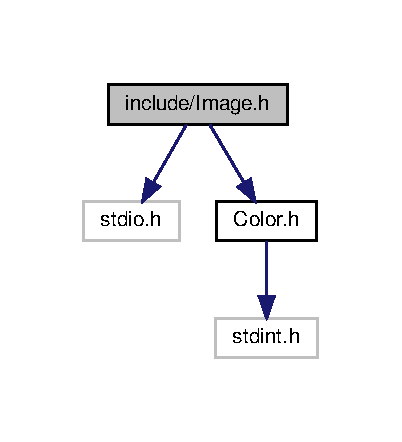
\includegraphics[width=193pt]{_image_8h__incl}
\end{center}
\end{figure}
This graph shows which files directly or indirectly include this file\+:\nopagebreak
\begin{figure}[H]
\begin{center}
\leavevmode
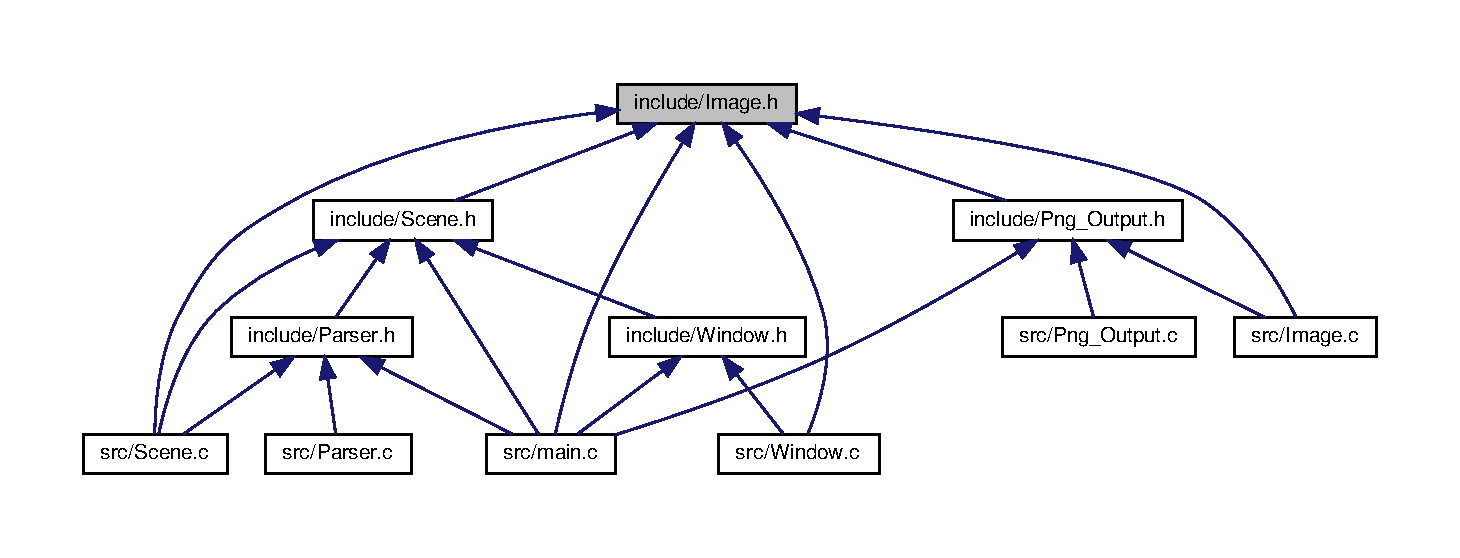
\includegraphics[width=350pt]{_image_8h__dep__incl}
\end{center}
\end{figure}
\subsection*{Data Structures}
\begin{DoxyCompactItemize}
\item 
struct \hyperlink{struct_image}{Image}
\begin{DoxyCompactList}\small\item\em represents an \hyperlink{struct_image}{Image} \end{DoxyCompactList}\end{DoxyCompactItemize}
\subsection*{Typedefs}
\begin{DoxyCompactItemize}
\item 
typedef struct \hyperlink{struct_image}{Image} \hyperlink{_image_8h_acf12205a65321baefe5174db248f56f6}{Image}
\end{DoxyCompactItemize}
\subsection*{Functions}
\begin{DoxyCompactItemize}
\item 
\hyperlink{struct_image}{Image} $\ast$ \hyperlink{_image_8h_a90385dabc85b0af27497eed57a2372ee}{new\+Image} (int w, int h)
\begin{DoxyCompactList}\small\item\em create a image of size w x h \end{DoxyCompactList}\item 
void \hyperlink{_image_8h_a404a3ccd4a05f939d24646a64ecd2539}{free\+Image} (\hyperlink{struct_image}{Image} $\ast$image)
\begin{DoxyCompactList}\small\item\em free all the memory alocated by the image \end{DoxyCompactList}\item 
int \hyperlink{_image_8h_a4f8a59fa9ff8f8bc8dc8345f79acc69e}{write\+Image\+P\+PM} (\hyperlink{struct_image}{Image} $\ast$I, const char $\ast$export\+\_\+file\+\_\+name)
\begin{DoxyCompactList}\small\item\em export image to P\+PM \end{DoxyCompactList}\item 
int \hyperlink{_image_8h_aa26105e7379206b03980ebf579c67e18}{write\+Image\+P\+NG} (\hyperlink{struct_image}{Image} $\ast$I, const char $\ast$export\+\_\+file\+\_\+name)
\begin{DoxyCompactList}\small\item\em export image to P\+NG \end{DoxyCompactList}\item 
\hyperlink{struct_image}{Image} $\ast$ \hyperlink{_image_8h_a95fd9ecea4469c4f839116feadda8105}{clone\+Image} (\hyperlink{struct_image}{Image} $\ast$src)
\begin{DoxyCompactList}\small\item\em clone a image (this function make memory allocation) \end{DoxyCompactList}\item 
int \hyperlink{_image_8h_a029610b9f61710fba7717f81abc831eb}{cpy\+Image} (\hyperlink{struct_image}{Image} $\ast$dest, \hyperlink{struct_image}{Image} $\ast$src)
\begin{DoxyCompactList}\small\item\em copy an image to another \end{DoxyCompactList}\item 
int \hyperlink{_image_8h_abc536a624594d32cf629d15e727e1304}{Image\+Set\+Pixel} (\hyperlink{struct_image}{Image} $\ast$image, const \hyperlink{struct_color}{Color} $\ast$p, int row, int column)
\begin{DoxyCompactList}\small\item\em sets the color of the given pixel \end{DoxyCompactList}\item 
int \hyperlink{_image_8h_a7cdcf43538a56567ec37ed007ff6df3e}{Image\+Get\+Pixel} (const \hyperlink{struct_image}{Image} $\ast$img, \hyperlink{struct_color}{Color} $\ast$res, int row, int column)
\begin{DoxyCompactList}\small\item\em gets the color of a given pixel \end{DoxyCompactList}\item 
void \hyperlink{_image_8h_a12fca6dfb14c74382e06366ad01a47e7}{progressive\+Ray} (int render, \hyperlink{struct_image}{Image} $\ast$dest, \hyperlink{struct_image}{Image} $\ast$comming, \hyperlink{struct_image}{Image} $\ast$old)
\begin{DoxyCompactList}\small\item\em make a progressive\+Ray on two image \end{DoxyCompactList}\end{DoxyCompactItemize}


\subsection{Detailed Description}
represents R\+GB image 

\begin{DoxyAuthor}{Author}
Jean-\/\+Manuel E\+R\+I\+A\+LC -\/ Hadjer D\+J\+E\+R\+R\+O\+U\+MI 
\end{DoxyAuthor}
\begin{DoxyVersion}{Version}
0.\+1 
\end{DoxyVersion}
\begin{DoxyDate}{Date}
11 juin 2020
\end{DoxyDate}
contains R\+GB type image and fonctions related to it 

\subsection{Typedef Documentation}
\mbox{\Hypertarget{_image_8h_acf12205a65321baefe5174db248f56f6}\label{_image_8h_acf12205a65321baefe5174db248f56f6}} 
\index{Image.\+h@{Image.\+h}!Image@{Image}}
\index{Image@{Image}!Image.\+h@{Image.\+h}}
\subsubsection{\texorpdfstring{Image}{Image}}
{\footnotesize\ttfamily typedef struct \hyperlink{struct_image}{Image} \hyperlink{struct_image}{Image}}



\subsection{Function Documentation}
\mbox{\Hypertarget{_image_8h_a95fd9ecea4469c4f839116feadda8105}\label{_image_8h_a95fd9ecea4469c4f839116feadda8105}} 
\index{Image.\+h@{Image.\+h}!clone\+Image@{clone\+Image}}
\index{clone\+Image@{clone\+Image}!Image.\+h@{Image.\+h}}
\subsubsection{\texorpdfstring{clone\+Image()}{cloneImage()}}
{\footnotesize\ttfamily \hyperlink{struct_image}{Image} $\ast$ clone\+Image (\begin{DoxyParamCaption}\item[{\hyperlink{struct_image}{Image} $\ast$}]{src }\end{DoxyParamCaption})}



clone a image (this function make memory allocation) 


\begin{DoxyParams}{Parameters}
{\em src} & the image to clone \\
\hline
\end{DoxyParams}
\begin{DoxyReturn}{Returns}
the address of the cloned image~\newline
 N\+U\+LL if a memory allocation occurs or src == N\+U\+LL 
\end{DoxyReturn}
\mbox{\Hypertarget{_image_8h_a029610b9f61710fba7717f81abc831eb}\label{_image_8h_a029610b9f61710fba7717f81abc831eb}} 
\index{Image.\+h@{Image.\+h}!cpy\+Image@{cpy\+Image}}
\index{cpy\+Image@{cpy\+Image}!Image.\+h@{Image.\+h}}
\subsubsection{\texorpdfstring{cpy\+Image()}{cpyImage()}}
{\footnotesize\ttfamily int cpy\+Image (\begin{DoxyParamCaption}\item[{\hyperlink{struct_image}{Image} $\ast$}]{dest,  }\item[{\hyperlink{struct_image}{Image} $\ast$}]{src }\end{DoxyParamCaption})}



copy an image to another 


\begin{DoxyParams}{Parameters}
{\em dest} & the destination image \\
\hline
{\em src} & the source image \\
\hline
\end{DoxyParams}
\begin{DoxyReturn}{Returns}
1 if the image was successfully copied~\newline
 0 if a error occurs 
\end{DoxyReturn}
\mbox{\Hypertarget{_image_8h_a404a3ccd4a05f939d24646a64ecd2539}\label{_image_8h_a404a3ccd4a05f939d24646a64ecd2539}} 
\index{Image.\+h@{Image.\+h}!free\+Image@{free\+Image}}
\index{free\+Image@{free\+Image}!Image.\+h@{Image.\+h}}
\subsubsection{\texorpdfstring{free\+Image()}{freeImage()}}
{\footnotesize\ttfamily void free\+Image (\begin{DoxyParamCaption}\item[{\hyperlink{struct_image}{Image} $\ast$}]{image }\end{DoxyParamCaption})}



free all the memory alocated by the image 


\begin{DoxyParams}{Parameters}
{\em image} & the image to free \\
\hline
\end{DoxyParams}
\mbox{\Hypertarget{_image_8h_a7cdcf43538a56567ec37ed007ff6df3e}\label{_image_8h_a7cdcf43538a56567ec37ed007ff6df3e}} 
\index{Image.\+h@{Image.\+h}!Image\+Get\+Pixel@{Image\+Get\+Pixel}}
\index{Image\+Get\+Pixel@{Image\+Get\+Pixel}!Image.\+h@{Image.\+h}}
\subsubsection{\texorpdfstring{Image\+Get\+Pixel()}{ImageGetPixel()}}
{\footnotesize\ttfamily int Image\+Get\+Pixel (\begin{DoxyParamCaption}\item[{const \hyperlink{struct_image}{Image} $\ast$}]{img,  }\item[{\hyperlink{struct_color}{Color} $\ast$}]{res,  }\item[{int}]{row,  }\item[{int}]{column }\end{DoxyParamCaption})}



gets the color of a given pixel 


\begin{DoxyParams}{Parameters}
{\em img} & the image \\
\hline
{\em res} & the color of the pixel \\
\hline
{\em row} & the row of the pixel \\
\hline
{\em column} & the colomn of the pixel \\
\hline
\end{DoxyParams}
\begin{DoxyReturn}{Returns}
0 if a error occurs~\newline
 1 otherwise 
\end{DoxyReturn}
\mbox{\Hypertarget{_image_8h_abc536a624594d32cf629d15e727e1304}\label{_image_8h_abc536a624594d32cf629d15e727e1304}} 
\index{Image.\+h@{Image.\+h}!Image\+Set\+Pixel@{Image\+Set\+Pixel}}
\index{Image\+Set\+Pixel@{Image\+Set\+Pixel}!Image.\+h@{Image.\+h}}
\subsubsection{\texorpdfstring{Image\+Set\+Pixel()}{ImageSetPixel()}}
{\footnotesize\ttfamily int Image\+Set\+Pixel (\begin{DoxyParamCaption}\item[{\hyperlink{struct_image}{Image} $\ast$}]{image,  }\item[{const \hyperlink{struct_color}{Color} $\ast$}]{p,  }\item[{int}]{row,  }\item[{int}]{column }\end{DoxyParamCaption})}



sets the color of the given pixel 


\begin{DoxyParams}{Parameters}
{\em image} & the image to set \\
\hline
{\em p} & the new color of the pixel \\
\hline
{\em row} & the row of the pixel \\
\hline
{\em column} & the colomn of the pixel \\
\hline
\end{DoxyParams}
\begin{DoxyReturn}{Returns}
0 if a error occurs~\newline
 1 otherwise 
\end{DoxyReturn}
\mbox{\Hypertarget{_image_8h_a90385dabc85b0af27497eed57a2372ee}\label{_image_8h_a90385dabc85b0af27497eed57a2372ee}} 
\index{Image.\+h@{Image.\+h}!new\+Image@{new\+Image}}
\index{new\+Image@{new\+Image}!Image.\+h@{Image.\+h}}
\subsubsection{\texorpdfstring{new\+Image()}{newImage()}}
{\footnotesize\ttfamily \hyperlink{struct_image}{Image} $\ast$ new\+Image (\begin{DoxyParamCaption}\item[{int}]{w,  }\item[{int}]{h }\end{DoxyParamCaption})}



create a image of size w x h 


\begin{DoxyParams}{Parameters}
{\em w} & the width of the image to create \\
\hline
{\em h} & the height of the image to create \\
\hline
\end{DoxyParams}
\begin{DoxyReturn}{Returns}
the address of the created image~\newline
 N\+U\+LL if a image occurs(w $<$= 0 $\vert$$\vert$ h $<$= 0 or memory allocation error) 
\end{DoxyReturn}
\mbox{\Hypertarget{_image_8h_a12fca6dfb14c74382e06366ad01a47e7}\label{_image_8h_a12fca6dfb14c74382e06366ad01a47e7}} 
\index{Image.\+h@{Image.\+h}!progressive\+Ray@{progressive\+Ray}}
\index{progressive\+Ray@{progressive\+Ray}!Image.\+h@{Image.\+h}}
\subsubsection{\texorpdfstring{progressive\+Ray()}{progressiveRay()}}
{\footnotesize\ttfamily void progressive\+Ray (\begin{DoxyParamCaption}\item[{int}]{render,  }\item[{\hyperlink{struct_image}{Image} $\ast$}]{dest,  }\item[{\hyperlink{struct_image}{Image} $\ast$}]{comming,  }\item[{\hyperlink{struct_image}{Image} $\ast$}]{old }\end{DoxyParamCaption})}



make a progressive\+Ray on two image 


\begin{DoxyParams}{Parameters}
{\em render} & the render of the progressive\+Ray (between 1 and 9) \\
\hline
{\em dest} & the computed image \\
\hline
{\em comming} & the next image computed \\
\hline
{\em old} & the old image computed \\
\hline
\end{DoxyParams}
\mbox{\Hypertarget{_image_8h_aa26105e7379206b03980ebf579c67e18}\label{_image_8h_aa26105e7379206b03980ebf579c67e18}} 
\index{Image.\+h@{Image.\+h}!write\+Image\+P\+NG@{write\+Image\+P\+NG}}
\index{write\+Image\+P\+NG@{write\+Image\+P\+NG}!Image.\+h@{Image.\+h}}
\subsubsection{\texorpdfstring{write\+Image\+P\+N\+G()}{writeImagePNG()}}
{\footnotesize\ttfamily int write\+Image\+P\+NG (\begin{DoxyParamCaption}\item[{\hyperlink{struct_image}{Image} $\ast$}]{I,  }\item[{const char $\ast$}]{export\+\_\+file\+\_\+name }\end{DoxyParamCaption})}



export image to P\+NG 


\begin{DoxyParams}{Parameters}
{\em I} & the image to export \\
\hline
{\em export\+\_\+file\+\_\+name} & the path where the image should be exported \\
\hline
\end{DoxyParams}
\begin{DoxyReturn}{Returns}
1 if the image was successfully exported~\newline
 0 if a error occurs (I == N\+U\+LL $\vert$$\vert$ export\+\_\+file\+\_\+name == N\+U\+LL or the open of export\+\_\+file\+\_\+name fails) 
\end{DoxyReturn}
\mbox{\Hypertarget{_image_8h_a4f8a59fa9ff8f8bc8dc8345f79acc69e}\label{_image_8h_a4f8a59fa9ff8f8bc8dc8345f79acc69e}} 
\index{Image.\+h@{Image.\+h}!write\+Image\+P\+PM@{write\+Image\+P\+PM}}
\index{write\+Image\+P\+PM@{write\+Image\+P\+PM}!Image.\+h@{Image.\+h}}
\subsubsection{\texorpdfstring{write\+Image\+P\+P\+M()}{writeImagePPM()}}
{\footnotesize\ttfamily int write\+Image\+P\+PM (\begin{DoxyParamCaption}\item[{\hyperlink{struct_image}{Image} $\ast$}]{I,  }\item[{const char $\ast$}]{export\+\_\+file\+\_\+name }\end{DoxyParamCaption})}



export image to P\+PM 


\begin{DoxyParams}{Parameters}
{\em I} & the image to export \\
\hline
{\em export\+\_\+file\+\_\+name} & the path where the image should be exported \\
\hline
\end{DoxyParams}
\begin{DoxyReturn}{Returns}
1 if the image was successfully exported~\newline
 0 if a error occurs (I == N\+U\+LL $\vert$$\vert$ export\+\_\+file\+\_\+name == N\+U\+LL or the open of export\+\_\+file\+\_\+name fails) 
\end{DoxyReturn}

\hypertarget{_light_8h}{}\section{include/\+Light.h File Reference}
\label{_light_8h}\index{include/\+Light.\+h@{include/\+Light.\+h}}
{\ttfamily \#include \char`\"{}Point.\+h\char`\"{}}\newline
{\ttfamily \#include \char`\"{}Vecteur.\+h\char`\"{}}\newline
{\ttfamily \#include \char`\"{}Lst\+\_\+\+Object.\+h\char`\"{}}\newline
Include dependency graph for Light.\+h\+:\nopagebreak
\begin{figure}[H]
\begin{center}
\leavevmode
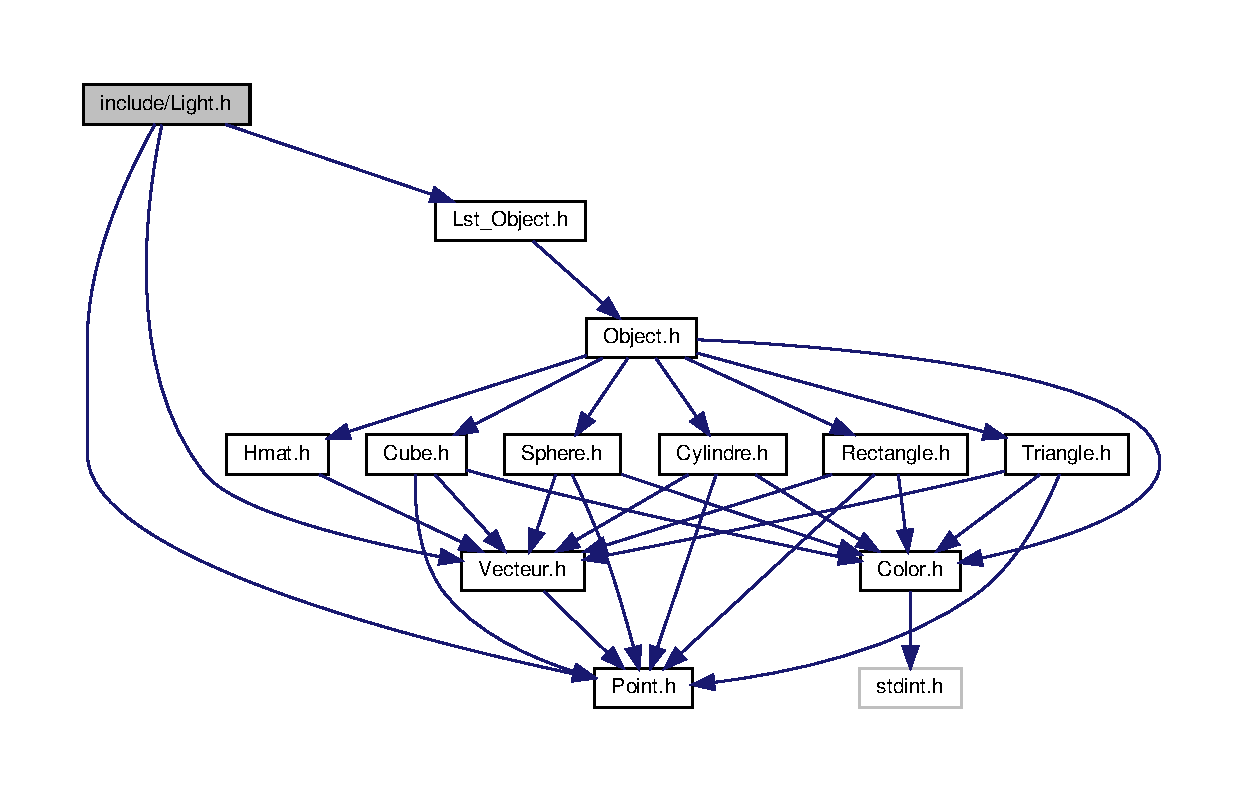
\includegraphics[width=350pt]{_light_8h__incl}
\end{center}
\end{figure}
This graph shows which files directly or indirectly include this file\+:\nopagebreak
\begin{figure}[H]
\begin{center}
\leavevmode
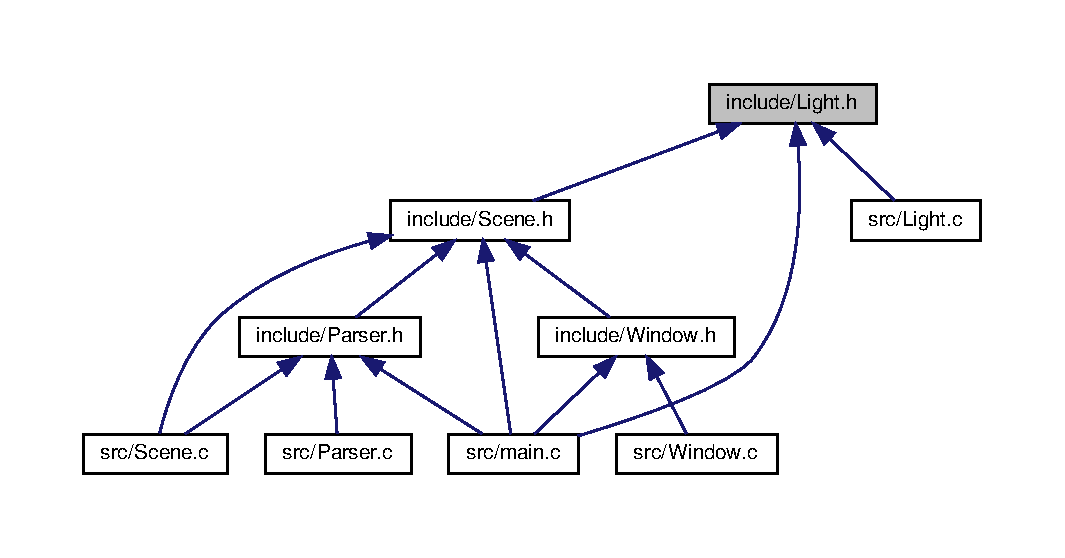
\includegraphics[width=350pt]{_light_8h__dep__incl}
\end{center}
\end{figure}
\subsection*{Data Structures}
\begin{DoxyCompactItemize}
\item 
struct \hyperlink{struct_source}{Source}
\begin{DoxyCompactList}\small\item\em a light source \end{DoxyCompactList}\item 
struct \hyperlink{struct__lst__point}{\+\_\+lst\+\_\+point}
\end{DoxyCompactItemize}
\subsection*{Typedefs}
\begin{DoxyCompactItemize}
\item 
typedef struct \hyperlink{struct__lst__point}{\+\_\+lst\+\_\+point} \hyperlink{_light_8h_ad242681e1717b8f774a276b2615c342c}{node\+\_\+\+Source}
\item 
typedef struct \hyperlink{struct__lst__point}{\+\_\+lst\+\_\+point} $\ast$ \hyperlink{_light_8h_aa56740bdfdc3237971604e047e2894fc}{lst\+\_\+\+Source}
\end{DoxyCompactItemize}
\subsection*{Functions}
\begin{DoxyCompactItemize}
\item 
int \hyperlink{_light_8h_a0ba575f751b8450bb4e7dc2932022587}{set\+Source} (\hyperlink{struct_source}{Source} $\ast$src, const \hyperlink{struct_point}{Point} $\ast$p, \hyperlink{g3x__transfo_8h_a89b2b23e407882a535d835574a7912e1}{double} intensity)
\begin{DoxyCompactList}\small\item\em sets a source with the specified parameters \end{DoxyCompactList}\item 
int \hyperlink{_light_8h_a0a9396997898e3cc6967fc19a8296d44}{add\+\_\+source} (\hyperlink{structlst___source}{lst\+\_\+\+Source} $\ast$lst, const \hyperlink{struct_source}{Source} $\ast$src)
\begin{DoxyCompactList}\small\item\em add a source to the list \end{DoxyCompactList}\item 
void \hyperlink{_light_8h_a256c1429a2986d4a7f3ab3d2bdc0ee43}{free\+\_\+lst\+\_\+\+Source} (\hyperlink{structlst___source}{lst\+\_\+\+Source} $\ast$lst)
\begin{DoxyCompactList}\small\item\em free all the memory alocated by a \hyperlink{structlst___source}{lst\+\_\+\+Source} \end{DoxyCompactList}\item 
int \hyperlink{_light_8h_ade2c2259c09a6f7b78ecb2a81dc426c5}{delta} (const \hyperlink{struct_source}{Source} $\ast$src, const \hyperlink{struct_point}{Point} $\ast$point, const \hyperlink{structlst___object}{lst\+\_\+\+Object} lst)
\begin{DoxyCompactList}\small\item\em check wether a point is illuminated by a source \end{DoxyCompactList}\item 
int \hyperlink{_light_8h_a62664dbe826347dc3feca688509ee54f}{Source\+Console\+Display} (const \hyperlink{struct_source}{Source} $\ast$s)
\begin{DoxyCompactList}\small\item\em print a source in the console \end{DoxyCompactList}\end{DoxyCompactItemize}


\subsection{Typedef Documentation}
\mbox{\Hypertarget{_light_8h_aa56740bdfdc3237971604e047e2894fc}\label{_light_8h_aa56740bdfdc3237971604e047e2894fc}} 
\index{Light.\+h@{Light.\+h}!lst\+\_\+\+Source@{lst\+\_\+\+Source}}
\index{lst\+\_\+\+Source@{lst\+\_\+\+Source}!Light.\+h@{Light.\+h}}
\subsubsection{\texorpdfstring{lst\+\_\+\+Source}{lst\_Source}}
{\footnotesize\ttfamily typedef struct \hyperlink{struct__lst__point}{\+\_\+lst\+\_\+point} $\ast$ \hyperlink{structlst___source}{lst\+\_\+\+Source}}

\mbox{\Hypertarget{_light_8h_ad242681e1717b8f774a276b2615c342c}\label{_light_8h_ad242681e1717b8f774a276b2615c342c}} 
\index{Light.\+h@{Light.\+h}!node\+\_\+\+Source@{node\+\_\+\+Source}}
\index{node\+\_\+\+Source@{node\+\_\+\+Source}!Light.\+h@{Light.\+h}}
\subsubsection{\texorpdfstring{node\+\_\+\+Source}{node\_Source}}
{\footnotesize\ttfamily typedef struct \hyperlink{struct__lst__point}{\+\_\+lst\+\_\+point} \hyperlink{_light_8h_ad242681e1717b8f774a276b2615c342c}{node\+\_\+\+Source}}



\subsection{Function Documentation}
\mbox{\Hypertarget{_light_8h_a0a9396997898e3cc6967fc19a8296d44}\label{_light_8h_a0a9396997898e3cc6967fc19a8296d44}} 
\index{Light.\+h@{Light.\+h}!add\+\_\+source@{add\+\_\+source}}
\index{add\+\_\+source@{add\+\_\+source}!Light.\+h@{Light.\+h}}
\subsubsection{\texorpdfstring{add\+\_\+source()}{add\_source()}}
{\footnotesize\ttfamily int add\+\_\+source (\begin{DoxyParamCaption}\item[{\hyperlink{structlst___source}{lst\+\_\+\+Source} $\ast$}]{lst,  }\item[{const \hyperlink{struct_source}{Source} $\ast$}]{src }\end{DoxyParamCaption})}



add a source to the list 


\begin{DoxyParams}{Parameters}
{\em lst} & the list \\
\hline
{\em src} & the the lignt source to add \\
\hline
\end{DoxyParams}
\begin{DoxyReturn}{Returns}
0 if a error occurs(lst == N\+U\+LL $\vert$$\vert$ src == N\+U\+LL or memory allocation error) 1 otherwise 
\end{DoxyReturn}
\mbox{\Hypertarget{_light_8h_ade2c2259c09a6f7b78ecb2a81dc426c5}\label{_light_8h_ade2c2259c09a6f7b78ecb2a81dc426c5}} 
\index{Light.\+h@{Light.\+h}!delta@{delta}}
\index{delta@{delta}!Light.\+h@{Light.\+h}}
\subsubsection{\texorpdfstring{delta()}{delta()}}
{\footnotesize\ttfamily int delta (\begin{DoxyParamCaption}\item[{const \hyperlink{struct_source}{Source} $\ast$}]{src,  }\item[{const \hyperlink{struct_point}{Point} $\ast$}]{point,  }\item[{const \hyperlink{structlst___object}{lst\+\_\+\+Object}}]{lst }\end{DoxyParamCaption})}



check wether a point is illuminated by a source 


\begin{DoxyParams}{Parameters}
{\em src} & a light source \\
\hline
{\em point} & a point \\
\hline
{\em lst} & the list of all objects of the scene \\
\hline
\end{DoxyParams}
\begin{DoxyReturn}{Returns}
-\/1 if a error occurs(src == N\+U\+LL $\vert$$\vert$ point == N\+U\+LL $\vert$$\vert$ lst == N\+U\+LL)~\newline
 0 if the point is not illuminated~\newline
 1 otherwise 
\end{DoxyReturn}
\mbox{\Hypertarget{_light_8h_a256c1429a2986d4a7f3ab3d2bdc0ee43}\label{_light_8h_a256c1429a2986d4a7f3ab3d2bdc0ee43}} 
\index{Light.\+h@{Light.\+h}!free\+\_\+lst\+\_\+\+Source@{free\+\_\+lst\+\_\+\+Source}}
\index{free\+\_\+lst\+\_\+\+Source@{free\+\_\+lst\+\_\+\+Source}!Light.\+h@{Light.\+h}}
\subsubsection{\texorpdfstring{free\+\_\+lst\+\_\+\+Source()}{free\_lst\_Source()}}
{\footnotesize\ttfamily void free\+\_\+lst\+\_\+\+Source (\begin{DoxyParamCaption}\item[{\hyperlink{structlst___source}{lst\+\_\+\+Source} $\ast$}]{lst }\end{DoxyParamCaption})}



free all the memory alocated by a \hyperlink{structlst___source}{lst\+\_\+\+Source} 


\begin{DoxyParams}{Parameters}
{\em lst} & the list to free \\
\hline
\end{DoxyParams}
\mbox{\Hypertarget{_light_8h_a0ba575f751b8450bb4e7dc2932022587}\label{_light_8h_a0ba575f751b8450bb4e7dc2932022587}} 
\index{Light.\+h@{Light.\+h}!set\+Source@{set\+Source}}
\index{set\+Source@{set\+Source}!Light.\+h@{Light.\+h}}
\subsubsection{\texorpdfstring{set\+Source()}{setSource()}}
{\footnotesize\ttfamily int set\+Source (\begin{DoxyParamCaption}\item[{\hyperlink{struct_source}{Source} $\ast$}]{src,  }\item[{const \hyperlink{struct_point}{Point} $\ast$}]{p,  }\item[{\hyperlink{g3x__transfo_8h_a89b2b23e407882a535d835574a7912e1}{double}}]{intensity }\end{DoxyParamCaption})}



sets a source with the specified parameters 


\begin{DoxyParams}{Parameters}
{\em src} & the light source to set \\
\hline
{\em p} & the position of the source \\
\hline
{\em intensity} & the intensity of the source \\
\hline
\end{DoxyParams}
\begin{DoxyReturn}{Returns}
0 if a error occurs(one parameter is N\+U\+L\+L)~\newline
 1 otherwise 
\end{DoxyReturn}
\mbox{\Hypertarget{_light_8h_a62664dbe826347dc3feca688509ee54f}\label{_light_8h_a62664dbe826347dc3feca688509ee54f}} 
\index{Light.\+h@{Light.\+h}!Source\+Console\+Display@{Source\+Console\+Display}}
\index{Source\+Console\+Display@{Source\+Console\+Display}!Light.\+h@{Light.\+h}}
\subsubsection{\texorpdfstring{Source\+Console\+Display()}{SourceConsoleDisplay()}}
{\footnotesize\ttfamily int Source\+Console\+Display (\begin{DoxyParamCaption}\item[{const \hyperlink{struct_source}{Source} $\ast$}]{s }\end{DoxyParamCaption})}



print a source in the console 


\begin{DoxyParams}{Parameters}
{\em s} & the light source to print \\
\hline
\end{DoxyParams}
\begin{DoxyReturn}{Returns}
0 if a error occurs(s == N\+U\+LL)~\newline
 1 otherwise 
\end{DoxyReturn}

\hypertarget{_lst___object_8h}{}\section{include/\+Lst\+\_\+\+Object.h File Reference}
\label{_lst___object_8h}\index{include/\+Lst\+\_\+\+Object.\+h@{include/\+Lst\+\_\+\+Object.\+h}}


represents a list of Objects (shapes)  


{\ttfamily \#include \char`\"{}Object.\+h\char`\"{}}\newline
Include dependency graph for Lst\+\_\+\+Object.\+h\+:\nopagebreak
\begin{figure}[H]
\begin{center}
\leavevmode
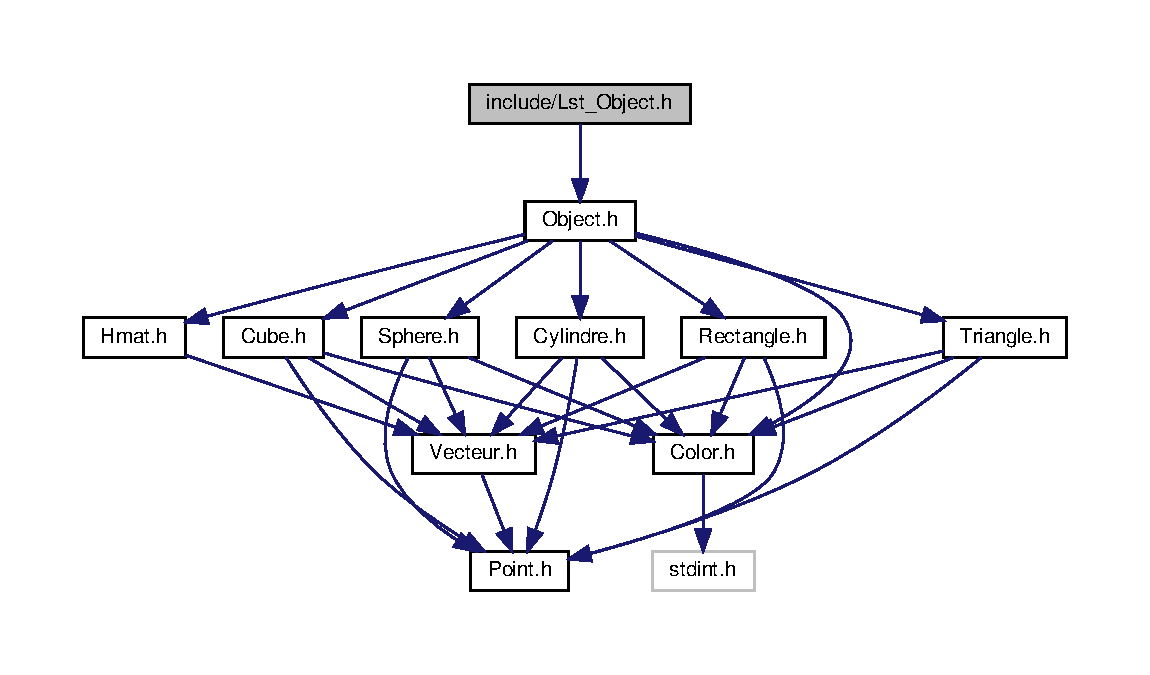
\includegraphics[width=350pt]{_lst___object_8h__incl}
\end{center}
\end{figure}
This graph shows which files directly or indirectly include this file\+:\nopagebreak
\begin{figure}[H]
\begin{center}
\leavevmode
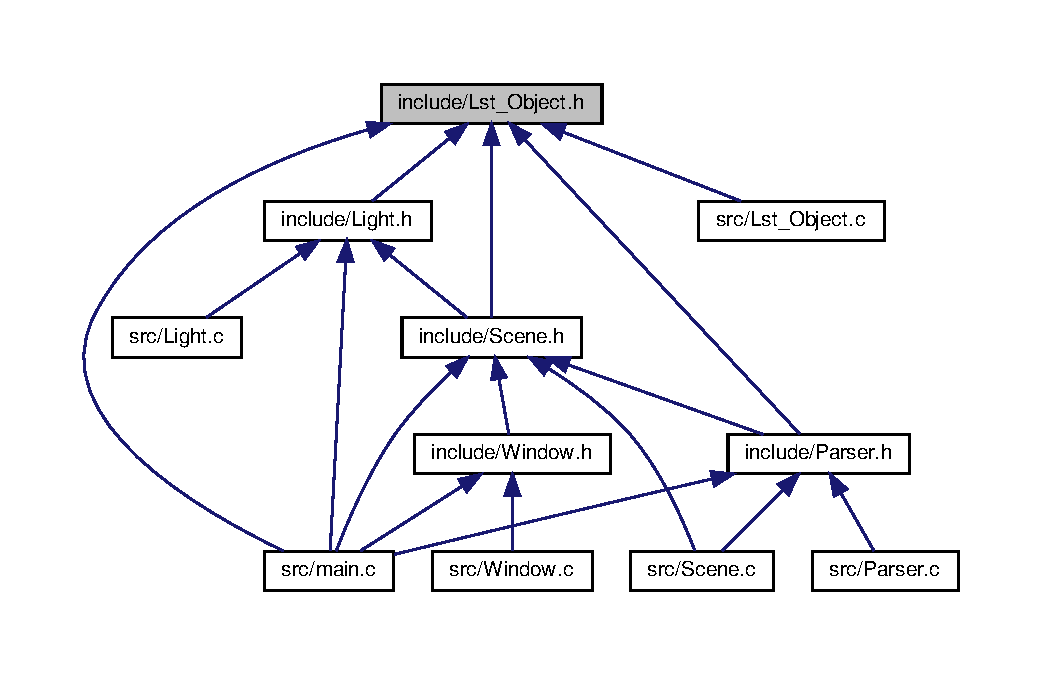
\includegraphics[width=350pt]{_lst___object_8h__dep__incl}
\end{center}
\end{figure}
\subsection*{Data Structures}
\begin{DoxyCompactItemize}
\item 
struct \hyperlink{struct__lst__obj}{\+\_\+lst\+\_\+obj}
\end{DoxyCompactItemize}
\subsection*{Typedefs}
\begin{DoxyCompactItemize}
\item 
typedef struct \hyperlink{struct__lst__obj}{\+\_\+lst\+\_\+obj} \hyperlink{_lst___object_8h_a1210e254271caff307db09ab53141206}{Object\+\_\+\+Node}
\item 
typedef struct \hyperlink{struct__lst__obj}{\+\_\+lst\+\_\+obj} $\ast$ \hyperlink{_lst___object_8h_a7b92649615b358e549b6be5551c5f09a}{lst\+\_\+\+Object}
\end{DoxyCompactItemize}
\subsection*{Functions}
\begin{DoxyCompactItemize}
\item 
int \hyperlink{_lst___object_8h_adf4f1899f0db47e4d39dc2f29743b80a}{lst\+\_\+\+Object\+\_\+add\+\_\+object} (\hyperlink{structlst___object}{lst\+\_\+\+Object} $\ast$lst, const \hyperlink{struct_object}{Object} $\ast$obj)
\begin{DoxyCompactList}\small\item\em add an object to the list \end{DoxyCompactList}\item 
void \hyperlink{_lst___object_8h_a1dd31100c0c57211501497d3707823a7}{lst\+\_\+\+Object\+\_\+free} (\hyperlink{structlst___object}{lst\+\_\+\+Object} $\ast$lst)
\begin{DoxyCompactList}\small\item\em free all the memory alocated by a \hyperlink{structlst___object}{lst\+\_\+\+Object} \end{DoxyCompactList}\end{DoxyCompactItemize}


\subsection{Detailed Description}
represents a list of Objects (shapes) 

\begin{DoxyAuthor}{Author}
Jean-\/\+Manuel E\+R\+I\+A\+LC -\/ Hadjer D\+J\+E\+R\+R\+O\+U\+MI 
\end{DoxyAuthor}
\begin{DoxyVersion}{Version}
0.\+1 
\end{DoxyVersion}
\begin{DoxyDate}{Date}
11 juin 2020
\end{DoxyDate}
represents a list of Objects (shapes) 

\subsection{Typedef Documentation}
\mbox{\Hypertarget{_lst___object_8h_a7b92649615b358e549b6be5551c5f09a}\label{_lst___object_8h_a7b92649615b358e549b6be5551c5f09a}} 
\index{Lst\+\_\+\+Object.\+h@{Lst\+\_\+\+Object.\+h}!lst\+\_\+\+Object@{lst\+\_\+\+Object}}
\index{lst\+\_\+\+Object@{lst\+\_\+\+Object}!Lst\+\_\+\+Object.\+h@{Lst\+\_\+\+Object.\+h}}
\subsubsection{\texorpdfstring{lst\+\_\+\+Object}{lst\_Object}}
{\footnotesize\ttfamily typedef struct \hyperlink{struct__lst__obj}{\+\_\+lst\+\_\+obj} $\ast$ \hyperlink{structlst___object}{lst\+\_\+\+Object}}

\mbox{\Hypertarget{_lst___object_8h_a1210e254271caff307db09ab53141206}\label{_lst___object_8h_a1210e254271caff307db09ab53141206}} 
\index{Lst\+\_\+\+Object.\+h@{Lst\+\_\+\+Object.\+h}!Object\+\_\+\+Node@{Object\+\_\+\+Node}}
\index{Object\+\_\+\+Node@{Object\+\_\+\+Node}!Lst\+\_\+\+Object.\+h@{Lst\+\_\+\+Object.\+h}}
\subsubsection{\texorpdfstring{Object\+\_\+\+Node}{Object\_Node}}
{\footnotesize\ttfamily typedef struct \hyperlink{struct__lst__obj}{\+\_\+lst\+\_\+obj} \hyperlink{_lst___object_8h_a1210e254271caff307db09ab53141206}{Object\+\_\+\+Node}}



\subsection{Function Documentation}
\mbox{\Hypertarget{_lst___object_8h_adf4f1899f0db47e4d39dc2f29743b80a}\label{_lst___object_8h_adf4f1899f0db47e4d39dc2f29743b80a}} 
\index{Lst\+\_\+\+Object.\+h@{Lst\+\_\+\+Object.\+h}!lst\+\_\+\+Object\+\_\+add\+\_\+object@{lst\+\_\+\+Object\+\_\+add\+\_\+object}}
\index{lst\+\_\+\+Object\+\_\+add\+\_\+object@{lst\+\_\+\+Object\+\_\+add\+\_\+object}!Lst\+\_\+\+Object.\+h@{Lst\+\_\+\+Object.\+h}}
\subsubsection{\texorpdfstring{lst\+\_\+\+Object\+\_\+add\+\_\+object()}{lst\_Object\_add\_object()}}
{\footnotesize\ttfamily int lst\+\_\+\+Object\+\_\+add\+\_\+object (\begin{DoxyParamCaption}\item[{\hyperlink{structlst___object}{lst\+\_\+\+Object} $\ast$}]{lst,  }\item[{const \hyperlink{struct_object}{Object} $\ast$}]{obj }\end{DoxyParamCaption})}



add an object to the list 


\begin{DoxyParams}{Parameters}
{\em lst} & the list \\
\hline
{\em obj} & the object to add \\
\hline
\end{DoxyParams}
\begin{DoxyReturn}{Returns}
0 if a error occurs(lst == N\+U\+LL $\vert$$\vert$ obj == N\+U\+LL or memory allocation error) 1 otherwise 
\end{DoxyReturn}
\mbox{\Hypertarget{_lst___object_8h_a1dd31100c0c57211501497d3707823a7}\label{_lst___object_8h_a1dd31100c0c57211501497d3707823a7}} 
\index{Lst\+\_\+\+Object.\+h@{Lst\+\_\+\+Object.\+h}!lst\+\_\+\+Object\+\_\+free@{lst\+\_\+\+Object\+\_\+free}}
\index{lst\+\_\+\+Object\+\_\+free@{lst\+\_\+\+Object\+\_\+free}!Lst\+\_\+\+Object.\+h@{Lst\+\_\+\+Object.\+h}}
\subsubsection{\texorpdfstring{lst\+\_\+\+Object\+\_\+free()}{lst\_Object\_free()}}
{\footnotesize\ttfamily void lst\+\_\+\+Object\+\_\+free (\begin{DoxyParamCaption}\item[{\hyperlink{structlst___object}{lst\+\_\+\+Object} $\ast$}]{lst }\end{DoxyParamCaption})}



free all the memory alocated by a \hyperlink{structlst___object}{lst\+\_\+\+Object} 


\begin{DoxyParams}{Parameters}
{\em lst} & the list to free \\
\hline
\end{DoxyParams}

\hypertarget{_object_8h}{}\section{include/\+Object.h File Reference}
\label{_object_8h}\index{include/\+Object.\+h@{include/\+Object.\+h}}
{\ttfamily \#include \char`\"{}Hmat.\+h\char`\"{}}\newline
{\ttfamily \#include \char`\"{}Cube.\+h\char`\"{}}\newline
{\ttfamily \#include \char`\"{}Sphere.\+h\char`\"{}}\newline
{\ttfamily \#include \char`\"{}Cylindre.\+h\char`\"{}}\newline
{\ttfamily \#include \char`\"{}Rectangle.\+h\char`\"{}}\newline
{\ttfamily \#include \char`\"{}Triangle.\+h\char`\"{}}\newline
{\ttfamily \#include \char`\"{}Color.\+h\char`\"{}}\newline
Include dependency graph for Object.\+h\+:\nopagebreak
\begin{figure}[H]
\begin{center}
\leavevmode
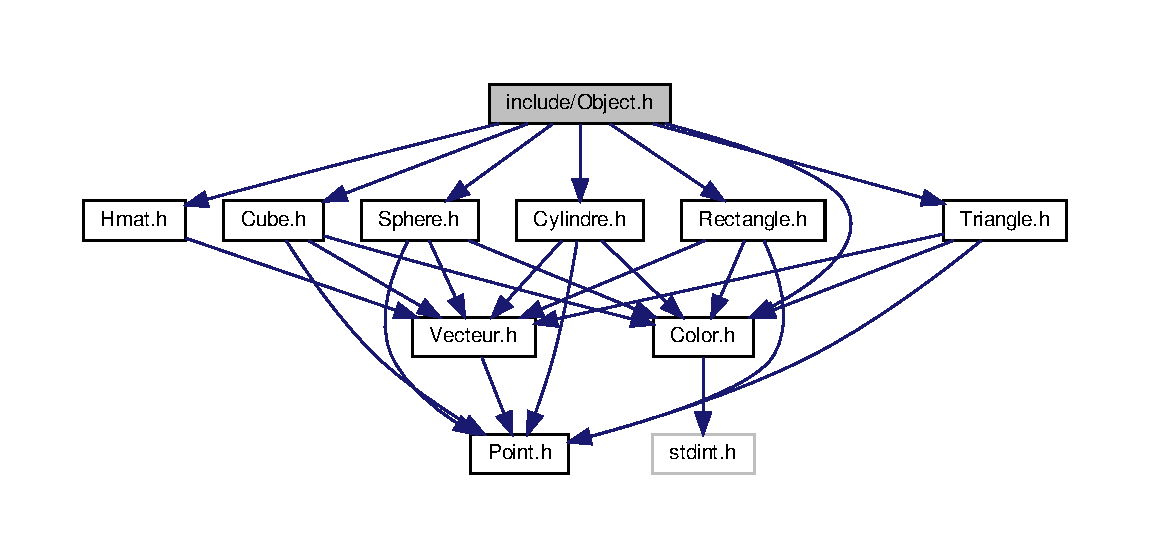
\includegraphics[width=350pt]{_object_8h__incl}
\end{center}
\end{figure}
This graph shows which files directly or indirectly include this file\+:\nopagebreak
\begin{figure}[H]
\begin{center}
\leavevmode
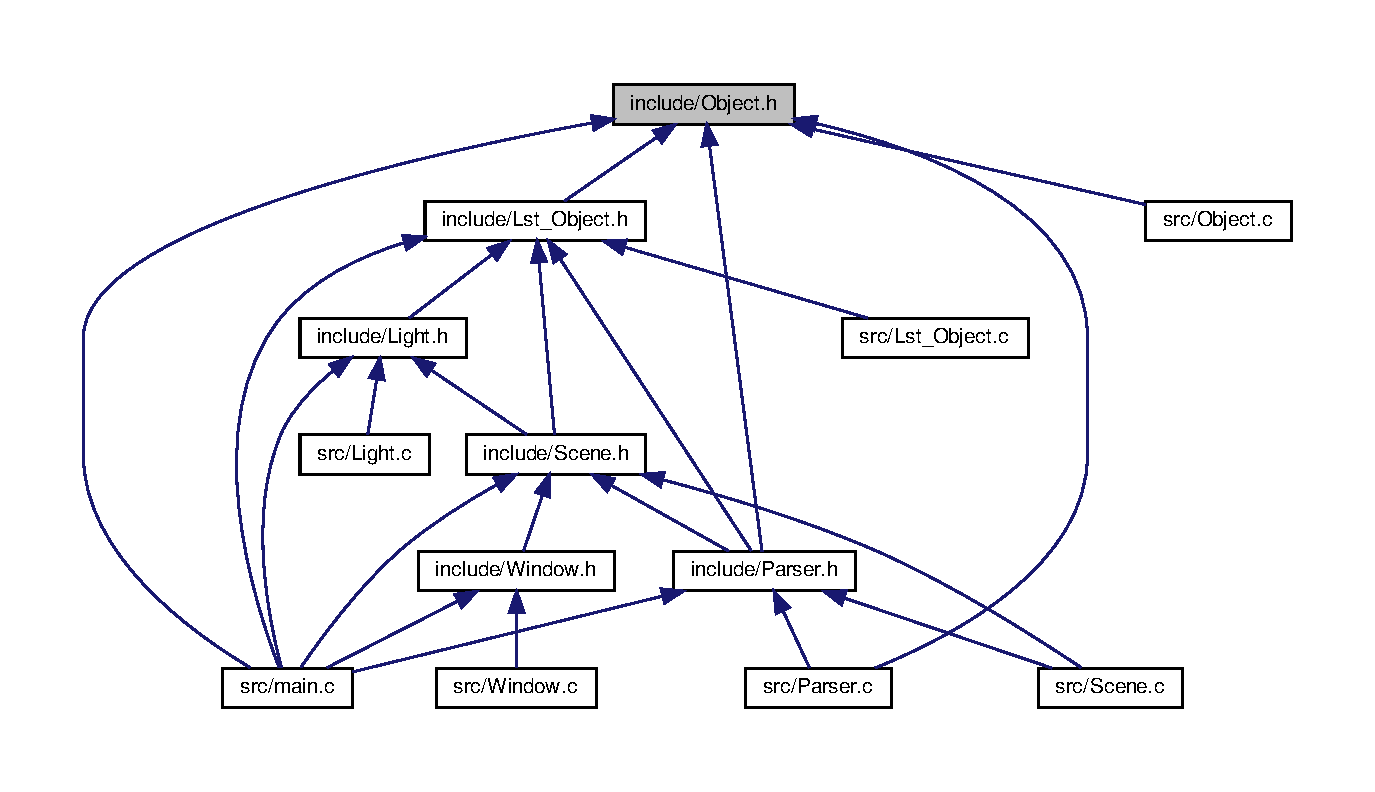
\includegraphics[width=350pt]{_object_8h__dep__incl}
\end{center}
\end{figure}
\subsection*{Data Structures}
\begin{DoxyCompactItemize}
\item 
struct \hyperlink{struct_object}{Object}
\begin{DoxyCompactList}\small\item\em an object \end{DoxyCompactList}\end{DoxyCompactItemize}
\subsection*{Macros}
\begin{DoxyCompactItemize}
\item 
\#define \hyperlink{_object_8h_aa48bb8f73122cf63876c27cbe830c581}{T\+Y\+P\+E\+\_\+\+O\+B\+J\+E\+C\+T\+\_\+\+S\+I\+ZE}~6
\end{DoxyCompactItemize}
\subsection*{Typedefs}
\begin{DoxyCompactItemize}
\item 
typedef enum \hyperlink{_object_8h_af3ec464aa442c2d0bd0c227fda28a8be}{T\+Y\+P\+E\+\_\+\+O\+B\+J\+E\+CT} \hyperlink{_object_8h_a27b04329eb8da9faf17427ce24dc59e5}{T\+Y\+P\+E\+\_\+\+O\+B\+J\+E\+CT}
\end{DoxyCompactItemize}
\subsection*{Enumerations}
\begin{DoxyCompactItemize}
\item 
enum \hyperlink{_object_8h_af3ec464aa442c2d0bd0c227fda28a8be}{T\+Y\+P\+E\+\_\+\+O\+B\+J\+E\+CT} \{ \newline
\hyperlink{_object_8h_af3ec464aa442c2d0bd0c227fda28a8bea09b024ff449662360c66ce18d20096fa}{U\+N\+K\+N\+OW}, 
\hyperlink{_object_8h_af3ec464aa442c2d0bd0c227fda28a8bead9ff273a12ff18b3e1b900080aadd1ea}{C\+U\+BE}, 
\hyperlink{_object_8h_af3ec464aa442c2d0bd0c227fda28a8beaf853bc4ffa031fb42cb4298b0c2106b9}{C\+Y\+L\+I\+N\+D\+RE}, 
\hyperlink{_object_8h_af3ec464aa442c2d0bd0c227fda28a8beae552ab0a96c0384a6e918e726b7f6102}{R\+E\+C\+T\+A\+N\+G\+LE}, 
\newline
\hyperlink{_object_8h_af3ec464aa442c2d0bd0c227fda28a8beaae4f0962d104ea473feec5598689316d}{S\+P\+H\+E\+RE}, 
\hyperlink{_object_8h_af3ec464aa442c2d0bd0c227fda28a8bea2fd33892864d1c342d3bead2f2d9ad56}{T\+R\+I\+A\+N\+G\+LE}
 \}\begin{DoxyCompactList}\small\item\em enumerate all types of objects \end{DoxyCompactList}
\end{DoxyCompactItemize}
\subsection*{Functions}
\begin{DoxyCompactItemize}
\item 
\hyperlink{_object_8h_af3ec464aa442c2d0bd0c227fda28a8be}{T\+Y\+P\+E\+\_\+\+O\+B\+J\+E\+CT} \hyperlink{_object_8h_ab32f8d726dda9fdb876eec5aefd57f42}{string\+\_\+to\+\_\+\+T\+Y\+P\+E\+\_\+\+O\+B\+J\+E\+CT} (char $\ast$object\+\_\+name)
\begin{DoxyCompactList}\small\item\em transforms the name of a object e.\+g \hyperlink{struct_sphere}{Sphere} to his T\+Y\+P\+E\+\_\+\+O\+B\+J\+E\+CT enum \end{DoxyCompactList}\item 
int \hyperlink{_object_8h_a1a22ac87616cdbe196512ef1b73ae5f0}{translate} (\hyperlink{struct_object}{Object} $\ast$obj, const \hyperlink{struct_vecteur}{Vecteur} $\ast$v)
\begin{DoxyCompactList}\small\item\em translates an object with the vector v \end{DoxyCompactList}\item 
int \hyperlink{_object_8h_a350a211d1f76f1a76c4dc3cfd4f34c33}{rescale} (\hyperlink{struct_object}{Object} $\ast$obj, \hyperlink{g3x__transfo_8h_a89b2b23e407882a535d835574a7912e1}{double} a, \hyperlink{g3x__transfo_8h_a89b2b23e407882a535d835574a7912e1}{double} b, \hyperlink{g3x__transfo_8h_a89b2b23e407882a535d835574a7912e1}{double} c)
\begin{DoxyCompactList}\small\item\em recale an object with specified parameters \end{DoxyCompactList}\item 
int \hyperlink{_object_8h_af4348e62b05f2570bb442cfb121c0341}{rotate\+\_\+x} (\hyperlink{struct_object}{Object} $\ast$obj, const \hyperlink{struct_vecteur}{Vecteur} $\ast$u, const \hyperlink{struct_vecteur}{Vecteur} $\ast$v)
\begin{DoxyCompactList}\small\item\em rotate an object with angle (u, v) around the ox axis \end{DoxyCompactList}\item 
int \hyperlink{_object_8h_ac0c36f5f4faa52bf80eea7b747eed60b}{rotate\+\_\+y} (\hyperlink{struct_object}{Object} $\ast$obj, const \hyperlink{struct_vecteur}{Vecteur} $\ast$u, const \hyperlink{struct_vecteur}{Vecteur} $\ast$v)
\begin{DoxyCompactList}\small\item\em rotate an object with angle (u, v) around the oy axis \end{DoxyCompactList}\item 
int \hyperlink{_object_8h_a83a6004b2e5803e7696326c1ecc3d5ce}{rotate\+\_\+z} (\hyperlink{struct_object}{Object} $\ast$obj, const \hyperlink{struct_vecteur}{Vecteur} $\ast$u, const \hyperlink{struct_vecteur}{Vecteur} $\ast$v)
\begin{DoxyCompactList}\small\item\em rotate an object with angle (u, v) around the oz axis \end{DoxyCompactList}\item 
int \hyperlink{_object_8h_a241c87f1a0ab2e6d1dcea47f7c7dfe89}{Object\+From\+Cube} (\hyperlink{struct_object}{Object} $\ast$object, const \hyperlink{struct_cube}{Cube} $\ast$cube)
\begin{DoxyCompactList}\small\item\em create an \hyperlink{struct_object}{Object} from a given \hyperlink{struct_cube}{Cube} \end{DoxyCompactList}\item 
int \hyperlink{_object_8h_aa0b25ac5933cbb73775aee217c94bff7}{Object\+From\+Cylindre} (\hyperlink{struct_object}{Object} $\ast$object, const \hyperlink{struct_cylindre}{Cylindre} $\ast$cylindre)
\begin{DoxyCompactList}\small\item\em create an \hyperlink{struct_object}{Object} from a given Cylinder \end{DoxyCompactList}\item 
int \hyperlink{_object_8h_a9bbc408cde820bda9e040e07948171b2}{Object\+From\+Rectangle} (\hyperlink{struct_object}{Object} $\ast$object, const \hyperlink{struct_rectangle}{Rectangle} $\ast$rectangle)
\begin{DoxyCompactList}\small\item\em create an \hyperlink{struct_object}{Object} from a given \hyperlink{struct_rectangle}{Rectangle} \end{DoxyCompactList}\item 
int \hyperlink{_object_8h_ad28d6620bda753a3908abf2704c538db}{Object\+From\+Sphere} (\hyperlink{struct_object}{Object} $\ast$object, const \hyperlink{struct_sphere}{Sphere} $\ast$sphere)
\begin{DoxyCompactList}\small\item\em create an \hyperlink{struct_object}{Object} from a given \hyperlink{struct_sphere}{Sphere} \end{DoxyCompactList}\item 
int \hyperlink{_object_8h_a0c9fdcf1b9f04f4c44a879e191673c2c}{Object\+From\+Triangle} (\hyperlink{struct_object}{Object} $\ast$object, const \hyperlink{struct_triangle}{Triangle} $\ast$triangle)
\begin{DoxyCompactList}\small\item\em create an \hyperlink{struct_object}{Object} from a given \hyperlink{struct_triangle}{Triangle} \end{DoxyCompactList}\item 
void \hyperlink{_object_8h_af40b8e36625f2ede9a38ab2f7d74d6f0}{Object\+Copy} (\hyperlink{struct_object}{Object} $\ast$dest, const \hyperlink{struct_object}{Object} $\ast$src)
\end{DoxyCompactItemize}


\subsection{Macro Definition Documentation}
\mbox{\Hypertarget{_object_8h_aa48bb8f73122cf63876c27cbe830c581}\label{_object_8h_aa48bb8f73122cf63876c27cbe830c581}} 
\index{Object.\+h@{Object.\+h}!T\+Y\+P\+E\+\_\+\+O\+B\+J\+E\+C\+T\+\_\+\+S\+I\+ZE@{T\+Y\+P\+E\+\_\+\+O\+B\+J\+E\+C\+T\+\_\+\+S\+I\+ZE}}
\index{T\+Y\+P\+E\+\_\+\+O\+B\+J\+E\+C\+T\+\_\+\+S\+I\+ZE@{T\+Y\+P\+E\+\_\+\+O\+B\+J\+E\+C\+T\+\_\+\+S\+I\+ZE}!Object.\+h@{Object.\+h}}
\subsubsection{\texorpdfstring{T\+Y\+P\+E\+\_\+\+O\+B\+J\+E\+C\+T\+\_\+\+S\+I\+ZE}{TYPE\_OBJECT\_SIZE}}
{\footnotesize\ttfamily \#define T\+Y\+P\+E\+\_\+\+O\+B\+J\+E\+C\+T\+\_\+\+S\+I\+ZE~6}



\subsection{Typedef Documentation}
\mbox{\Hypertarget{_object_8h_a27b04329eb8da9faf17427ce24dc59e5}\label{_object_8h_a27b04329eb8da9faf17427ce24dc59e5}} 
\index{Object.\+h@{Object.\+h}!T\+Y\+P\+E\+\_\+\+O\+B\+J\+E\+CT@{T\+Y\+P\+E\+\_\+\+O\+B\+J\+E\+CT}}
\index{T\+Y\+P\+E\+\_\+\+O\+B\+J\+E\+CT@{T\+Y\+P\+E\+\_\+\+O\+B\+J\+E\+CT}!Object.\+h@{Object.\+h}}
\subsubsection{\texorpdfstring{T\+Y\+P\+E\+\_\+\+O\+B\+J\+E\+CT}{TYPE\_OBJECT}}
{\footnotesize\ttfamily typedef enum \hyperlink{_object_8h_af3ec464aa442c2d0bd0c227fda28a8be}{T\+Y\+P\+E\+\_\+\+O\+B\+J\+E\+CT}  \hyperlink{_object_8h_af3ec464aa442c2d0bd0c227fda28a8be}{T\+Y\+P\+E\+\_\+\+O\+B\+J\+E\+CT}}



\subsection{Enumeration Type Documentation}
\mbox{\Hypertarget{_object_8h_af3ec464aa442c2d0bd0c227fda28a8be}\label{_object_8h_af3ec464aa442c2d0bd0c227fda28a8be}} 
\index{Object.\+h@{Object.\+h}!T\+Y\+P\+E\+\_\+\+O\+B\+J\+E\+CT@{T\+Y\+P\+E\+\_\+\+O\+B\+J\+E\+CT}}
\index{T\+Y\+P\+E\+\_\+\+O\+B\+J\+E\+CT@{T\+Y\+P\+E\+\_\+\+O\+B\+J\+E\+CT}!Object.\+h@{Object.\+h}}
\subsubsection{\texorpdfstring{T\+Y\+P\+E\+\_\+\+O\+B\+J\+E\+CT}{TYPE\_OBJECT}}
{\footnotesize\ttfamily enum \hyperlink{_object_8h_af3ec464aa442c2d0bd0c227fda28a8be}{T\+Y\+P\+E\+\_\+\+O\+B\+J\+E\+CT}}



enumerate all types of objects 

\hyperlink{struct_object}{Object} can be \hyperlink{struct_cube}{Cube}, Cylinder, \hyperlink{struct_rectangle}{Rectangle}, \hyperlink{struct_sphere}{Sphere} or \hyperlink{struct_triangle}{Triangle} \begin{DoxyEnumFields}{Enumerator}
\raisebox{\heightof{T}}[0pt][0pt]{\index{U\+N\+K\+N\+OW@{U\+N\+K\+N\+OW}!Object.\+h@{Object.\+h}}\index{Object.\+h@{Object.\+h}!U\+N\+K\+N\+OW@{U\+N\+K\+N\+OW}}}\mbox{\Hypertarget{_object_8h_af3ec464aa442c2d0bd0c227fda28a8bea09b024ff449662360c66ce18d20096fa}\label{_object_8h_af3ec464aa442c2d0bd0c227fda28a8bea09b024ff449662360c66ce18d20096fa}} 
U\+N\+K\+N\+OW&\\
\hline

\raisebox{\heightof{T}}[0pt][0pt]{\index{C\+U\+BE@{C\+U\+BE}!Object.\+h@{Object.\+h}}\index{Object.\+h@{Object.\+h}!C\+U\+BE@{C\+U\+BE}}}\mbox{\Hypertarget{_object_8h_af3ec464aa442c2d0bd0c227fda28a8bead9ff273a12ff18b3e1b900080aadd1ea}\label{_object_8h_af3ec464aa442c2d0bd0c227fda28a8bead9ff273a12ff18b3e1b900080aadd1ea}} 
C\+U\+BE&\\
\hline

\raisebox{\heightof{T}}[0pt][0pt]{\index{C\+Y\+L\+I\+N\+D\+RE@{C\+Y\+L\+I\+N\+D\+RE}!Object.\+h@{Object.\+h}}\index{Object.\+h@{Object.\+h}!C\+Y\+L\+I\+N\+D\+RE@{C\+Y\+L\+I\+N\+D\+RE}}}\mbox{\Hypertarget{_object_8h_af3ec464aa442c2d0bd0c227fda28a8beaf853bc4ffa031fb42cb4298b0c2106b9}\label{_object_8h_af3ec464aa442c2d0bd0c227fda28a8beaf853bc4ffa031fb42cb4298b0c2106b9}} 
C\+Y\+L\+I\+N\+D\+RE&\\
\hline

\raisebox{\heightof{T}}[0pt][0pt]{\index{R\+E\+C\+T\+A\+N\+G\+LE@{R\+E\+C\+T\+A\+N\+G\+LE}!Object.\+h@{Object.\+h}}\index{Object.\+h@{Object.\+h}!R\+E\+C\+T\+A\+N\+G\+LE@{R\+E\+C\+T\+A\+N\+G\+LE}}}\mbox{\Hypertarget{_object_8h_af3ec464aa442c2d0bd0c227fda28a8beae552ab0a96c0384a6e918e726b7f6102}\label{_object_8h_af3ec464aa442c2d0bd0c227fda28a8beae552ab0a96c0384a6e918e726b7f6102}} 
R\+E\+C\+T\+A\+N\+G\+LE&\\
\hline

\raisebox{\heightof{T}}[0pt][0pt]{\index{S\+P\+H\+E\+RE@{S\+P\+H\+E\+RE}!Object.\+h@{Object.\+h}}\index{Object.\+h@{Object.\+h}!S\+P\+H\+E\+RE@{S\+P\+H\+E\+RE}}}\mbox{\Hypertarget{_object_8h_af3ec464aa442c2d0bd0c227fda28a8beaae4f0962d104ea473feec5598689316d}\label{_object_8h_af3ec464aa442c2d0bd0c227fda28a8beaae4f0962d104ea473feec5598689316d}} 
S\+P\+H\+E\+RE&\\
\hline

\raisebox{\heightof{T}}[0pt][0pt]{\index{T\+R\+I\+A\+N\+G\+LE@{T\+R\+I\+A\+N\+G\+LE}!Object.\+h@{Object.\+h}}\index{Object.\+h@{Object.\+h}!T\+R\+I\+A\+N\+G\+LE@{T\+R\+I\+A\+N\+G\+LE}}}\mbox{\Hypertarget{_object_8h_af3ec464aa442c2d0bd0c227fda28a8bea2fd33892864d1c342d3bead2f2d9ad56}\label{_object_8h_af3ec464aa442c2d0bd0c227fda28a8bea2fd33892864d1c342d3bead2f2d9ad56}} 
T\+R\+I\+A\+N\+G\+LE&\\
\hline

\end{DoxyEnumFields}


\subsection{Function Documentation}
\mbox{\Hypertarget{_object_8h_af40b8e36625f2ede9a38ab2f7d74d6f0}\label{_object_8h_af40b8e36625f2ede9a38ab2f7d74d6f0}} 
\index{Object.\+h@{Object.\+h}!Object\+Copy@{Object\+Copy}}
\index{Object\+Copy@{Object\+Copy}!Object.\+h@{Object.\+h}}
\subsubsection{\texorpdfstring{Object\+Copy()}{ObjectCopy()}}
{\footnotesize\ttfamily void Object\+Copy (\begin{DoxyParamCaption}\item[{\hyperlink{struct_object}{Object} $\ast$}]{dest,  }\item[{const \hyperlink{struct_object}{Object} $\ast$}]{src }\end{DoxyParamCaption})}

\mbox{\Hypertarget{_object_8h_a241c87f1a0ab2e6d1dcea47f7c7dfe89}\label{_object_8h_a241c87f1a0ab2e6d1dcea47f7c7dfe89}} 
\index{Object.\+h@{Object.\+h}!Object\+From\+Cube@{Object\+From\+Cube}}
\index{Object\+From\+Cube@{Object\+From\+Cube}!Object.\+h@{Object.\+h}}
\subsubsection{\texorpdfstring{Object\+From\+Cube()}{ObjectFromCube()}}
{\footnotesize\ttfamily int Object\+From\+Cube (\begin{DoxyParamCaption}\item[{\hyperlink{struct_object}{Object} $\ast$}]{object,  }\item[{const \hyperlink{struct_cube}{Cube} $\ast$}]{cube }\end{DoxyParamCaption})}



create an \hyperlink{struct_object}{Object} from a given \hyperlink{struct_cube}{Cube} 


\begin{DoxyParams}{Parameters}
{\em object} & the object to create \\
\hline
{\em cube} & the given cube \\
\hline
\end{DoxyParams}
\begin{DoxyReturn}{Returns}
0 if a error occurs(one parameter is N\+U\+L\+L)~\newline
 1 otherwise 
\end{DoxyReturn}
\mbox{\Hypertarget{_object_8h_aa0b25ac5933cbb73775aee217c94bff7}\label{_object_8h_aa0b25ac5933cbb73775aee217c94bff7}} 
\index{Object.\+h@{Object.\+h}!Object\+From\+Cylindre@{Object\+From\+Cylindre}}
\index{Object\+From\+Cylindre@{Object\+From\+Cylindre}!Object.\+h@{Object.\+h}}
\subsubsection{\texorpdfstring{Object\+From\+Cylindre()}{ObjectFromCylindre()}}
{\footnotesize\ttfamily int Object\+From\+Cylindre (\begin{DoxyParamCaption}\item[{\hyperlink{struct_object}{Object} $\ast$}]{object,  }\item[{const \hyperlink{struct_cylindre}{Cylindre} $\ast$}]{cylindre }\end{DoxyParamCaption})}



create an \hyperlink{struct_object}{Object} from a given Cylinder 


\begin{DoxyParams}{Parameters}
{\em object} & the object to create \\
\hline
{\em cylindre} & the given cylinder \\
\hline
\end{DoxyParams}
\begin{DoxyReturn}{Returns}
0 if a error occurs(one parameter is N\+U\+L\+L)~\newline
 1 otherwise 
\end{DoxyReturn}
\mbox{\Hypertarget{_object_8h_a9bbc408cde820bda9e040e07948171b2}\label{_object_8h_a9bbc408cde820bda9e040e07948171b2}} 
\index{Object.\+h@{Object.\+h}!Object\+From\+Rectangle@{Object\+From\+Rectangle}}
\index{Object\+From\+Rectangle@{Object\+From\+Rectangle}!Object.\+h@{Object.\+h}}
\subsubsection{\texorpdfstring{Object\+From\+Rectangle()}{ObjectFromRectangle()}}
{\footnotesize\ttfamily int Object\+From\+Rectangle (\begin{DoxyParamCaption}\item[{\hyperlink{struct_object}{Object} $\ast$}]{object,  }\item[{const \hyperlink{struct_rectangle}{Rectangle} $\ast$}]{rectangle }\end{DoxyParamCaption})}



create an \hyperlink{struct_object}{Object} from a given \hyperlink{struct_rectangle}{Rectangle} 


\begin{DoxyParams}{Parameters}
{\em object} & the object to create \\
\hline
{\em rectangle} & the given rectangle \\
\hline
\end{DoxyParams}
\begin{DoxyReturn}{Returns}
0 if a error occurs(one parameter is N\+U\+L\+L)~\newline
 1 otherwise 
\end{DoxyReturn}
\mbox{\Hypertarget{_object_8h_ad28d6620bda753a3908abf2704c538db}\label{_object_8h_ad28d6620bda753a3908abf2704c538db}} 
\index{Object.\+h@{Object.\+h}!Object\+From\+Sphere@{Object\+From\+Sphere}}
\index{Object\+From\+Sphere@{Object\+From\+Sphere}!Object.\+h@{Object.\+h}}
\subsubsection{\texorpdfstring{Object\+From\+Sphere()}{ObjectFromSphere()}}
{\footnotesize\ttfamily int Object\+From\+Sphere (\begin{DoxyParamCaption}\item[{\hyperlink{struct_object}{Object} $\ast$}]{object,  }\item[{const \hyperlink{struct_sphere}{Sphere} $\ast$}]{sphere }\end{DoxyParamCaption})}



create an \hyperlink{struct_object}{Object} from a given \hyperlink{struct_sphere}{Sphere} 


\begin{DoxyParams}{Parameters}
{\em object} & the object to create \\
\hline
{\em sphere} & the given sphere \\
\hline
\end{DoxyParams}
\begin{DoxyReturn}{Returns}
0 if a error occurs(one parameter is N\+U\+L\+L)~\newline
 1 otherwise 
\end{DoxyReturn}
\mbox{\Hypertarget{_object_8h_a0c9fdcf1b9f04f4c44a879e191673c2c}\label{_object_8h_a0c9fdcf1b9f04f4c44a879e191673c2c}} 
\index{Object.\+h@{Object.\+h}!Object\+From\+Triangle@{Object\+From\+Triangle}}
\index{Object\+From\+Triangle@{Object\+From\+Triangle}!Object.\+h@{Object.\+h}}
\subsubsection{\texorpdfstring{Object\+From\+Triangle()}{ObjectFromTriangle()}}
{\footnotesize\ttfamily int Object\+From\+Triangle (\begin{DoxyParamCaption}\item[{\hyperlink{struct_object}{Object} $\ast$}]{object,  }\item[{const \hyperlink{struct_triangle}{Triangle} $\ast$}]{triangle }\end{DoxyParamCaption})}



create an \hyperlink{struct_object}{Object} from a given \hyperlink{struct_triangle}{Triangle} 


\begin{DoxyParams}{Parameters}
{\em object} & the object to create \\
\hline
{\em triangle} & the given triangle \\
\hline
\end{DoxyParams}
\begin{DoxyReturn}{Returns}
0 if a error occurs(one parameter is N\+U\+L\+L)~\newline
 1 otherwise 
\end{DoxyReturn}
\mbox{\Hypertarget{_object_8h_a350a211d1f76f1a76c4dc3cfd4f34c33}\label{_object_8h_a350a211d1f76f1a76c4dc3cfd4f34c33}} 
\index{Object.\+h@{Object.\+h}!rescale@{rescale}}
\index{rescale@{rescale}!Object.\+h@{Object.\+h}}
\subsubsection{\texorpdfstring{rescale()}{rescale()}}
{\footnotesize\ttfamily int rescale (\begin{DoxyParamCaption}\item[{\hyperlink{struct_object}{Object} $\ast$}]{obj,  }\item[{\hyperlink{g3x__transfo_8h_a89b2b23e407882a535d835574a7912e1}{double}}]{a,  }\item[{\hyperlink{g3x__transfo_8h_a89b2b23e407882a535d835574a7912e1}{double}}]{b,  }\item[{\hyperlink{g3x__transfo_8h_a89b2b23e407882a535d835574a7912e1}{double}}]{c }\end{DoxyParamCaption})}



recale an object with specified parameters 


\begin{DoxyParams}{Parameters}
{\em obj} & the object to translate \\
\hline
{\em a} & the ox parameter \\
\hline
{\em b} & the oy parameter \\
\hline
{\em c} & the oz parameter \\
\hline
\end{DoxyParams}
\begin{DoxyReturn}{Returns}
0 if a error occurs(obj == N\+U\+LL)~\newline
 1 otherwise 
\end{DoxyReturn}
\mbox{\Hypertarget{_object_8h_af4348e62b05f2570bb442cfb121c0341}\label{_object_8h_af4348e62b05f2570bb442cfb121c0341}} 
\index{Object.\+h@{Object.\+h}!rotate\+\_\+x@{rotate\+\_\+x}}
\index{rotate\+\_\+x@{rotate\+\_\+x}!Object.\+h@{Object.\+h}}
\subsubsection{\texorpdfstring{rotate\+\_\+x()}{rotate\_x()}}
{\footnotesize\ttfamily int rotate\+\_\+x (\begin{DoxyParamCaption}\item[{\hyperlink{struct_object}{Object} $\ast$}]{obj,  }\item[{const \hyperlink{struct_vecteur}{Vecteur} $\ast$}]{u,  }\item[{const \hyperlink{struct_vecteur}{Vecteur} $\ast$}]{v }\end{DoxyParamCaption})}



rotate an object with angle (u, v) around the ox axis 


\begin{DoxyParams}{Parameters}
{\em obj} & the object to rotate \\
\hline
{\em u} & the first vector of the angle \\
\hline
{\em v} & the second vector of the angle \\
\hline
\end{DoxyParams}
\begin{DoxyReturn}{Returns}
0 if a error occurs(one parameter is N\+U\+L\+L)~\newline
 1 otherwise 
\end{DoxyReturn}
\mbox{\Hypertarget{_object_8h_ac0c36f5f4faa52bf80eea7b747eed60b}\label{_object_8h_ac0c36f5f4faa52bf80eea7b747eed60b}} 
\index{Object.\+h@{Object.\+h}!rotate\+\_\+y@{rotate\+\_\+y}}
\index{rotate\+\_\+y@{rotate\+\_\+y}!Object.\+h@{Object.\+h}}
\subsubsection{\texorpdfstring{rotate\+\_\+y()}{rotate\_y()}}
{\footnotesize\ttfamily int rotate\+\_\+y (\begin{DoxyParamCaption}\item[{\hyperlink{struct_object}{Object} $\ast$}]{obj,  }\item[{const \hyperlink{struct_vecteur}{Vecteur} $\ast$}]{u,  }\item[{const \hyperlink{struct_vecteur}{Vecteur} $\ast$}]{v }\end{DoxyParamCaption})}



rotate an object with angle (u, v) around the oy axis 


\begin{DoxyParams}{Parameters}
{\em obj} & the object to rotate \\
\hline
{\em u} & the first vector of the angle \\
\hline
{\em v} & the second vector of the angle \\
\hline
\end{DoxyParams}
\begin{DoxyReturn}{Returns}
0 if a error occurs(one parameter is N\+U\+L\+L)~\newline
 1 otherwise 
\end{DoxyReturn}
\mbox{\Hypertarget{_object_8h_a83a6004b2e5803e7696326c1ecc3d5ce}\label{_object_8h_a83a6004b2e5803e7696326c1ecc3d5ce}} 
\index{Object.\+h@{Object.\+h}!rotate\+\_\+z@{rotate\+\_\+z}}
\index{rotate\+\_\+z@{rotate\+\_\+z}!Object.\+h@{Object.\+h}}
\subsubsection{\texorpdfstring{rotate\+\_\+z()}{rotate\_z()}}
{\footnotesize\ttfamily int rotate\+\_\+z (\begin{DoxyParamCaption}\item[{\hyperlink{struct_object}{Object} $\ast$}]{obj,  }\item[{const \hyperlink{struct_vecteur}{Vecteur} $\ast$}]{u,  }\item[{const \hyperlink{struct_vecteur}{Vecteur} $\ast$}]{v }\end{DoxyParamCaption})}



rotate an object with angle (u, v) around the oz axis 


\begin{DoxyParams}{Parameters}
{\em obj} & the object to rotate \\
\hline
{\em u} & the first vector of the angle \\
\hline
{\em v} & the second vector of the angle \\
\hline
\end{DoxyParams}
\begin{DoxyReturn}{Returns}
0 if a error occurs(one parameter is N\+U\+L\+L)~\newline
 1 otherwise 
\end{DoxyReturn}
\mbox{\Hypertarget{_object_8h_ab32f8d726dda9fdb876eec5aefd57f42}\label{_object_8h_ab32f8d726dda9fdb876eec5aefd57f42}} 
\index{Object.\+h@{Object.\+h}!string\+\_\+to\+\_\+\+T\+Y\+P\+E\+\_\+\+O\+B\+J\+E\+CT@{string\+\_\+to\+\_\+\+T\+Y\+P\+E\+\_\+\+O\+B\+J\+E\+CT}}
\index{string\+\_\+to\+\_\+\+T\+Y\+P\+E\+\_\+\+O\+B\+J\+E\+CT@{string\+\_\+to\+\_\+\+T\+Y\+P\+E\+\_\+\+O\+B\+J\+E\+CT}!Object.\+h@{Object.\+h}}
\subsubsection{\texorpdfstring{string\+\_\+to\+\_\+\+T\+Y\+P\+E\+\_\+\+O\+B\+J\+E\+C\+T()}{string\_to\_TYPE\_OBJECT()}}
{\footnotesize\ttfamily \hyperlink{_object_8h_af3ec464aa442c2d0bd0c227fda28a8be}{T\+Y\+P\+E\+\_\+\+O\+B\+J\+E\+CT} string\+\_\+to\+\_\+\+T\+Y\+P\+E\+\_\+\+O\+B\+J\+E\+CT (\begin{DoxyParamCaption}\item[{char $\ast$}]{object\+\_\+name }\end{DoxyParamCaption})}



transforms the name of a object e.\+g \hyperlink{struct_sphere}{Sphere} to his T\+Y\+P\+E\+\_\+\+O\+B\+J\+E\+CT enum 


\begin{DoxyParams}{Parameters}
{\em object\+\_\+name} & the object name \\
\hline
\end{DoxyParams}
\begin{DoxyReturn}{Returns}
a T\+Y\+P\+E\+\_\+\+O\+B\+J\+E\+CT representing the object~\newline
 U\+N\+K\+N\+OW if an error occurs 
\end{DoxyReturn}
\mbox{\Hypertarget{_object_8h_a1a22ac87616cdbe196512ef1b73ae5f0}\label{_object_8h_a1a22ac87616cdbe196512ef1b73ae5f0}} 
\index{Object.\+h@{Object.\+h}!translate@{translate}}
\index{translate@{translate}!Object.\+h@{Object.\+h}}
\subsubsection{\texorpdfstring{translate()}{translate()}}
{\footnotesize\ttfamily int translate (\begin{DoxyParamCaption}\item[{\hyperlink{struct_object}{Object} $\ast$}]{obj,  }\item[{const \hyperlink{struct_vecteur}{Vecteur} $\ast$}]{v }\end{DoxyParamCaption})}



translates an object with the vector v 


\begin{DoxyParams}{Parameters}
{\em obj} & the object to translate \\
\hline
{\em v} & the translation vector \\
\hline
\end{DoxyParams}
\begin{DoxyReturn}{Returns}
0 if a error occurs(one parameter is N\+U\+L\+L)~\newline
 1 otherwise 
\end{DoxyReturn}

\hypertarget{_option_8h}{}\section{include/\+Option.h File Reference}
\label{_option_8h}\index{include/\+Option.\+h@{include/\+Option.\+h}}


represents the options specified by the user when launching the program  


This graph shows which files directly or indirectly include this file\+:\nopagebreak
\begin{figure}[H]
\begin{center}
\leavevmode
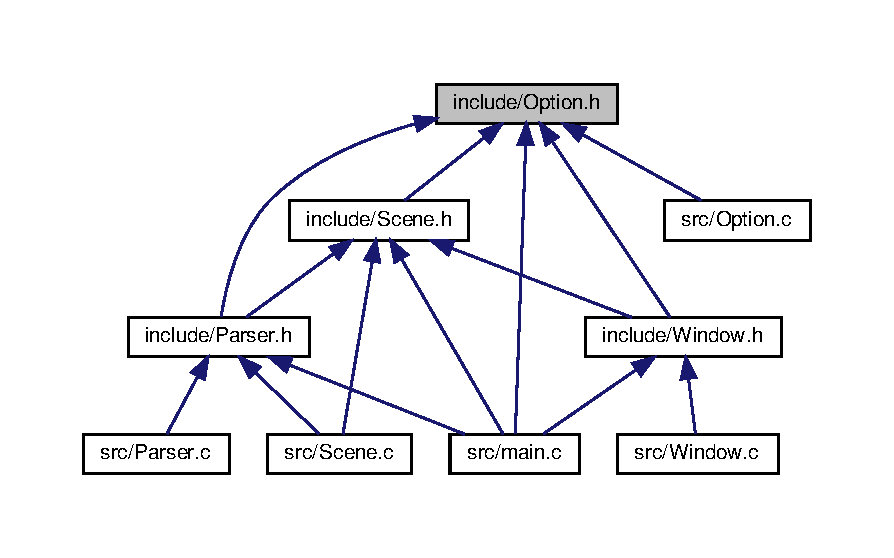
\includegraphics[width=350pt]{_option_8h__dep__incl}
\end{center}
\end{figure}
\subsection*{Data Structures}
\begin{DoxyCompactItemize}
\item 
struct \hyperlink{struct_option}{Option}
\begin{DoxyCompactList}\small\item\em options specified by the user \end{DoxyCompactList}\end{DoxyCompactItemize}
\subsection*{Functions}
\begin{DoxyCompactItemize}
\item 
int \hyperlink{_option_8h_a9503d21283d7b049cbd81dddc29aeb17}{want\+\_\+fast\+\_\+output\+\_\+scene} (const \hyperlink{struct_option}{Option} $\ast$options)
\begin{DoxyCompactList}\small\item\em tells if the user want the image of the scene without passing by a graphic window \end{DoxyCompactList}\end{DoxyCompactItemize}


\subsection{Detailed Description}
represents the options specified by the user when launching the program 

\begin{DoxyAuthor}{Author}
Jean-\/\+Manuel E\+R\+I\+A\+LC -\/ Hadjer D\+J\+E\+R\+R\+O\+U\+MI 
\end{DoxyAuthor}
\begin{DoxyVersion}{Version}
0.\+1 
\end{DoxyVersion}
\begin{DoxyDate}{Date}
11 juin 2020
\end{DoxyDate}
represents the options specified by the user when launching the program 

\subsection{Function Documentation}
\mbox{\Hypertarget{_option_8h_a9503d21283d7b049cbd81dddc29aeb17}\label{_option_8h_a9503d21283d7b049cbd81dddc29aeb17}} 
\index{Option.\+h@{Option.\+h}!want\+\_\+fast\+\_\+output\+\_\+scene@{want\+\_\+fast\+\_\+output\+\_\+scene}}
\index{want\+\_\+fast\+\_\+output\+\_\+scene@{want\+\_\+fast\+\_\+output\+\_\+scene}!Option.\+h@{Option.\+h}}
\subsubsection{\texorpdfstring{want\+\_\+fast\+\_\+output\+\_\+scene()}{want\_fast\_output\_scene()}}
{\footnotesize\ttfamily int want\+\_\+fast\+\_\+output\+\_\+scene (\begin{DoxyParamCaption}\item[{const \hyperlink{struct_option}{Option} $\ast$}]{options }\end{DoxyParamCaption})}



tells if the user want the image of the scene without passing by a graphic window 


\begin{DoxyParams}{Parameters}
{\em options} & options specified by the user \\
\hline
\end{DoxyParams}
\begin{DoxyReturn}{Returns}
1 if the user want the image of the scene without passing by a graphic window 0 otherwise
\end{DoxyReturn}
tells if the user want the image of the scene without passing by a graphic window 
\hypertarget{_parser_8h}{}\section{include/\+Parser.h File Reference}
\label{_parser_8h}\index{include/\+Parser.\+h@{include/\+Parser.\+h}}


contains the parser of user command line and a scene parser  


{\ttfamily \#include \char`\"{}Point.\+h\char`\"{}}\newline
{\ttfamily \#include \char`\"{}Cube.\+h\char`\"{}}\newline
{\ttfamily \#include \char`\"{}Sphere.\+h\char`\"{}}\newline
{\ttfamily \#include \char`\"{}Triangle.\+h\char`\"{}}\newline
{\ttfamily \#include \char`\"{}Rectangle.\+h\char`\"{}}\newline
{\ttfamily \#include \char`\"{}Cylindre.\+h\char`\"{}}\newline
{\ttfamily \#include \char`\"{}Camera.\+h\char`\"{}}\newline
{\ttfamily \#include \char`\"{}Object.\+h\char`\"{}}\newline
{\ttfamily \#include \char`\"{}Lst\+\_\+\+Object.\+h\char`\"{}}\newline
{\ttfamily \#include \char`\"{}Scene.\+h\char`\"{}}\newline
{\ttfamily \#include \char`\"{}Option.\+h\char`\"{}}\newline
Include dependency graph for Parser.\+h\+:\nopagebreak
\begin{figure}[H]
\begin{center}
\leavevmode
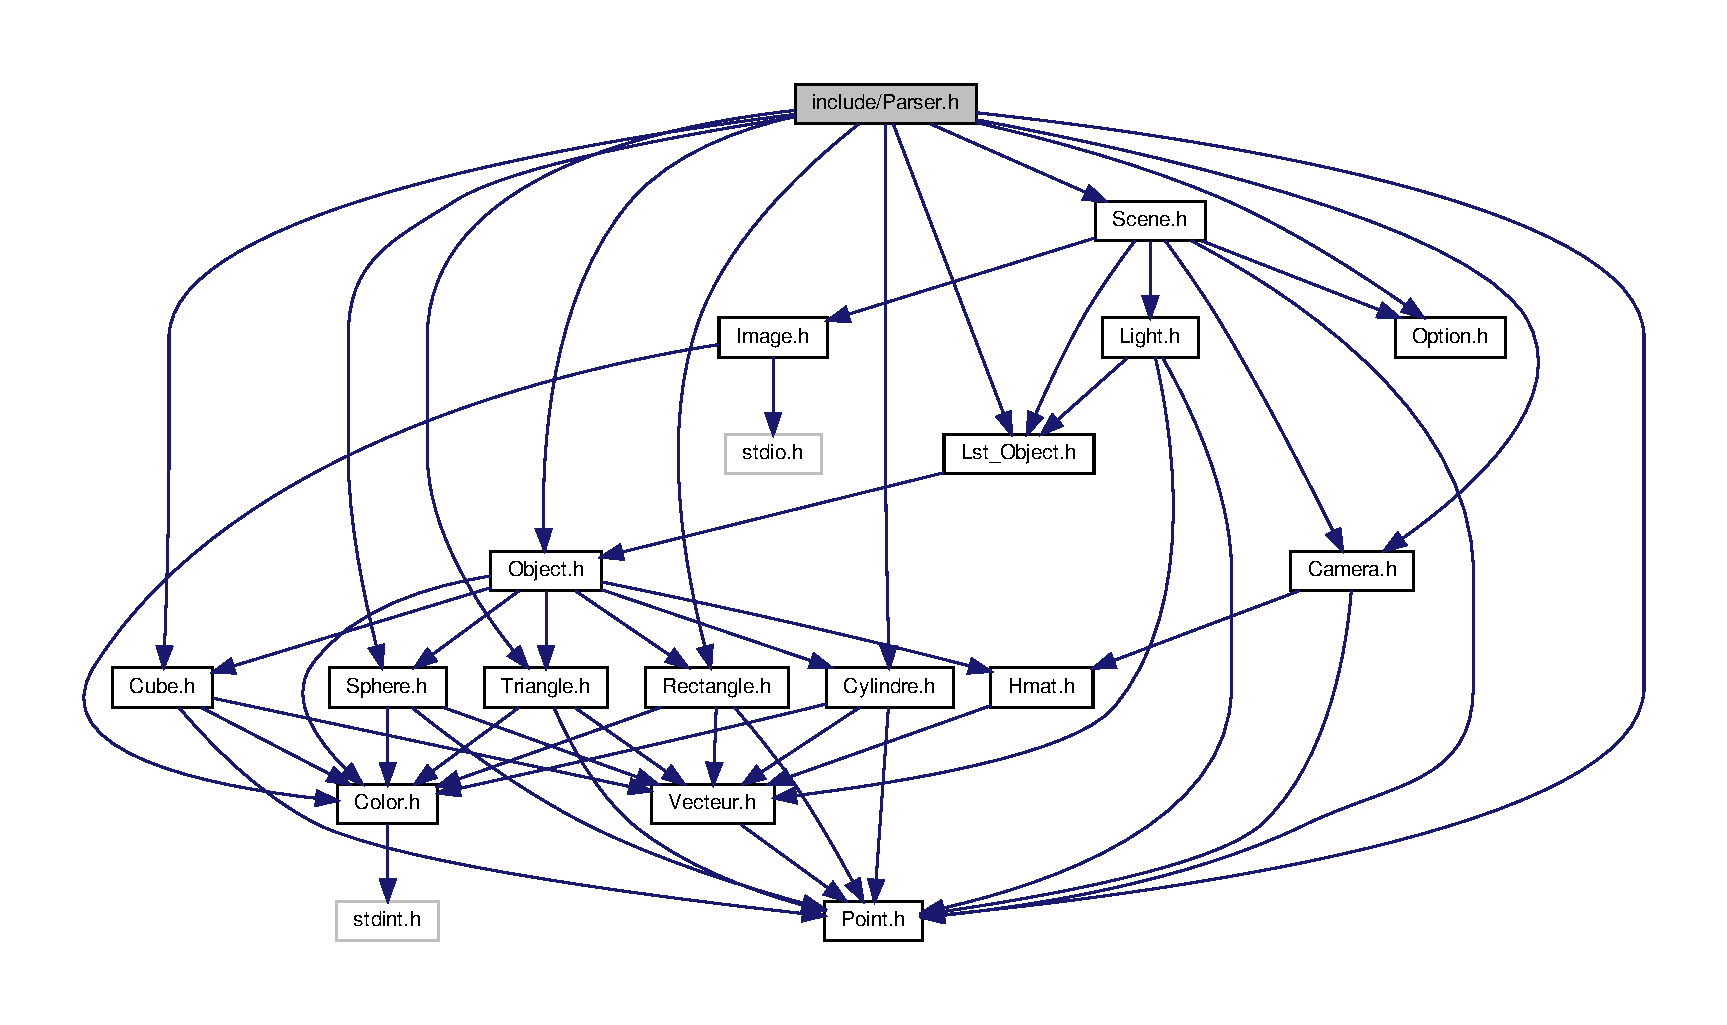
\includegraphics[width=350pt]{_parser_8h__incl}
\end{center}
\end{figure}
This graph shows which files directly or indirectly include this file\+:\nopagebreak
\begin{figure}[H]
\begin{center}
\leavevmode
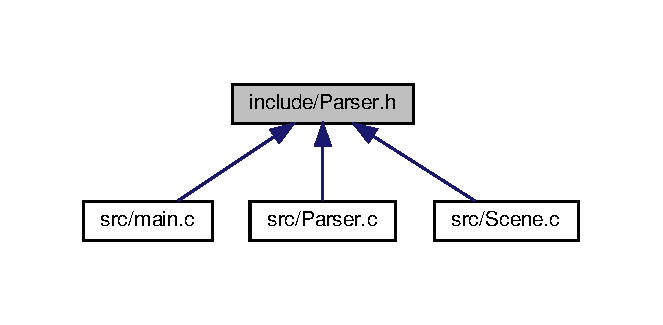
\includegraphics[width=318pt]{_parser_8h__dep__incl}
\end{center}
\end{figure}
\subsection*{Functions}
\begin{DoxyCompactItemize}
\item 
void \hyperlink{_parser_8h_a0b07aaf5d9b84d9c600364a1cb3a767d}{lray\+\_\+help} ()
\begin{DoxyCompactList}\small\item\em help message of lray program \end{DoxyCompactList}\item 
void \hyperlink{_parser_8h_ad23d60505728d0a0307d982a5f33f645}{lray\+\_\+usage} ()
\begin{DoxyCompactList}\small\item\em usage message of lray program \end{DoxyCompactList}\item 
int \hyperlink{_parser_8h_a011af2f67fb95e38b5839fe1fa6c452e}{parse\+\_\+args} (int argc, char $\ast$argv\mbox{[}$\,$\mbox{]}, \hyperlink{struct_option}{Option} $\ast$options)
\begin{DoxyCompactList}\small\item\em parse user arguments from the command line \end{DoxyCompactList}\item 
int \hyperlink{_parser_8h_a7d3e8a4a1e3ca923e8adb94a6a5c662d}{parse\+\_\+\+X\+M\+L\+\_\+scene} (const char $\ast$input\+\_\+path, \hyperlink{struct_scene}{Scene} $\ast$scene)
\begin{DoxyCompactList}\small\item\em parse a X\+ML scene \end{DoxyCompactList}\end{DoxyCompactItemize}


\subsection{Detailed Description}
contains the parser of user command line and a scene parser 

\begin{DoxyAuthor}{Author}
Jean-\/\+Manuel E\+R\+I\+A\+LC -\/ Hadjer D\+J\+E\+R\+R\+O\+U\+MI 
\end{DoxyAuthor}
\begin{DoxyVersion}{Version}
0.\+1 
\end{DoxyVersion}
\begin{DoxyDate}{Date}
11 juin 2020
\end{DoxyDate}
contains the parser of user command line and a scene parser 

\subsection{Function Documentation}
\mbox{\Hypertarget{_parser_8h_a0b07aaf5d9b84d9c600364a1cb3a767d}\label{_parser_8h_a0b07aaf5d9b84d9c600364a1cb3a767d}} 
\index{Parser.\+h@{Parser.\+h}!lray\+\_\+help@{lray\+\_\+help}}
\index{lray\+\_\+help@{lray\+\_\+help}!Parser.\+h@{Parser.\+h}}
\subsubsection{\texorpdfstring{lray\+\_\+help()}{lray\_help()}}
{\footnotesize\ttfamily void lray\+\_\+help (\begin{DoxyParamCaption}{ }\end{DoxyParamCaption})}



help message of lray program 

\mbox{\Hypertarget{_parser_8h_ad23d60505728d0a0307d982a5f33f645}\label{_parser_8h_ad23d60505728d0a0307d982a5f33f645}} 
\index{Parser.\+h@{Parser.\+h}!lray\+\_\+usage@{lray\+\_\+usage}}
\index{lray\+\_\+usage@{lray\+\_\+usage}!Parser.\+h@{Parser.\+h}}
\subsubsection{\texorpdfstring{lray\+\_\+usage()}{lray\_usage()}}
{\footnotesize\ttfamily void lray\+\_\+usage (\begin{DoxyParamCaption}{ }\end{DoxyParamCaption})}



usage message of lray program 

\mbox{\Hypertarget{_parser_8h_a011af2f67fb95e38b5839fe1fa6c452e}\label{_parser_8h_a011af2f67fb95e38b5839fe1fa6c452e}} 
\index{Parser.\+h@{Parser.\+h}!parse\+\_\+args@{parse\+\_\+args}}
\index{parse\+\_\+args@{parse\+\_\+args}!Parser.\+h@{Parser.\+h}}
\subsubsection{\texorpdfstring{parse\+\_\+args()}{parse\_args()}}
{\footnotesize\ttfamily int parse\+\_\+args (\begin{DoxyParamCaption}\item[{int}]{argc,  }\item[{char $\ast$}]{argv\mbox{[}$\,$\mbox{]},  }\item[{\hyperlink{struct_option}{Option} $\ast$}]{options }\end{DoxyParamCaption})}



parse user arguments from the command line 


\begin{DoxyParams}{Parameters}
{\em argc} & number of arguments \\
\hline
{\em argv} & all arguments \\
\hline
{\em options} & all options specified by user in a type \\
\hline
\end{DoxyParams}
\begin{DoxyReturn}{Returns}
0 if the parsing fails~\newline
 1 otherwise 
\end{DoxyReturn}
\mbox{\Hypertarget{_parser_8h_a7d3e8a4a1e3ca923e8adb94a6a5c662d}\label{_parser_8h_a7d3e8a4a1e3ca923e8adb94a6a5c662d}} 
\index{Parser.\+h@{Parser.\+h}!parse\+\_\+\+X\+M\+L\+\_\+scene@{parse\+\_\+\+X\+M\+L\+\_\+scene}}
\index{parse\+\_\+\+X\+M\+L\+\_\+scene@{parse\+\_\+\+X\+M\+L\+\_\+scene}!Parser.\+h@{Parser.\+h}}
\subsubsection{\texorpdfstring{parse\+\_\+\+X\+M\+L\+\_\+scene()}{parse\_XML\_scene()}}
{\footnotesize\ttfamily int parse\+\_\+\+X\+M\+L\+\_\+scene (\begin{DoxyParamCaption}\item[{const char $\ast$}]{input\+\_\+path,  }\item[{\hyperlink{struct_scene}{Scene} $\ast$}]{scene }\end{DoxyParamCaption})}



parse a X\+ML scene 


\begin{DoxyParams}{Parameters}
{\em input\+\_\+path} & path of the scene file \\
\hline
{\em scene} & the scene to build \\
\hline
\end{DoxyParams}
\begin{DoxyReturn}{Returns}
0 if a err occurs ( file not found or parsing error)~\newline
 1 successful parsing 
\end{DoxyReturn}

\hypertarget{_png___output_8h}{}\section{include/\+Png\+\_\+\+Output.h File Reference}
\label{_png___output_8h}\index{include/\+Png\+\_\+\+Output.\+h@{include/\+Png\+\_\+\+Output.\+h}}


export a \hyperlink{struct_image}{Image} in png  


{\ttfamily \#include \char`\"{}Image.\+h\char`\"{}}\newline
Include dependency graph for Png\+\_\+\+Output.\+h\+:\nopagebreak
\begin{figure}[H]
\begin{center}
\leavevmode
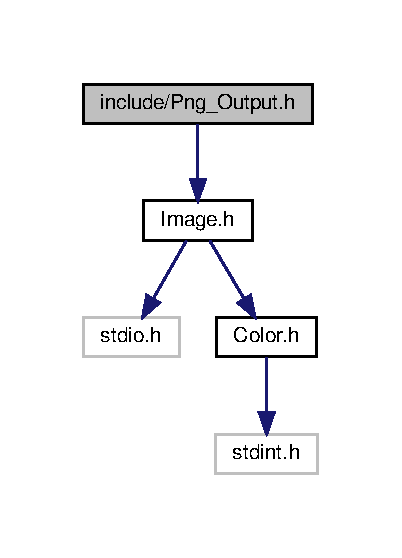
\includegraphics[width=193pt]{_png___output_8h__incl}
\end{center}
\end{figure}
This graph shows which files directly or indirectly include this file\+:\nopagebreak
\begin{figure}[H]
\begin{center}
\leavevmode
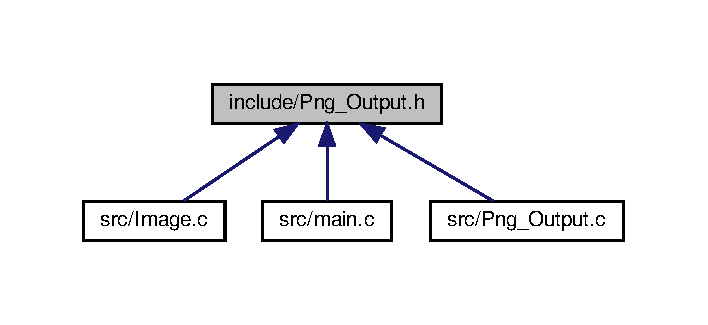
\includegraphics[width=340pt]{_png___output_8h__dep__incl}
\end{center}
\end{figure}
\subsection*{Functions}
\begin{DoxyCompactItemize}
\item 
int \hyperlink{_png___output_8h_ae9d911a4eee3b5d2ff5650baf555ca9f}{P\+N\+G\+\_\+output\+\_\+file} (const \hyperlink{struct_image}{Image} $\ast$I, const char $\ast$output\+\_\+path)
\begin{DoxyCompactList}\small\item\em exports a image in a file specified by a path in png format \end{DoxyCompactList}\end{DoxyCompactItemize}


\subsection{Detailed Description}
export a \hyperlink{struct_image}{Image} in png 

\begin{DoxyAuthor}{Author}
Jean-\/\+Manuel E\+R\+I\+A\+LC -\/ Hadjer D\+J\+E\+R\+R\+O\+U\+MI 
\end{DoxyAuthor}
\begin{DoxyVersion}{Version}
0.\+1 
\end{DoxyVersion}
\begin{DoxyDate}{Date}
11 juin 2020
\end{DoxyDate}
export a \hyperlink{struct_image}{Image} in png 

\subsection{Function Documentation}
\mbox{\Hypertarget{_png___output_8h_ae9d911a4eee3b5d2ff5650baf555ca9f}\label{_png___output_8h_ae9d911a4eee3b5d2ff5650baf555ca9f}} 
\index{Png\+\_\+\+Output.\+h@{Png\+\_\+\+Output.\+h}!P\+N\+G\+\_\+output\+\_\+file@{P\+N\+G\+\_\+output\+\_\+file}}
\index{P\+N\+G\+\_\+output\+\_\+file@{P\+N\+G\+\_\+output\+\_\+file}!Png\+\_\+\+Output.\+h@{Png\+\_\+\+Output.\+h}}
\subsubsection{\texorpdfstring{P\+N\+G\+\_\+output\+\_\+file()}{PNG\_output\_file()}}
{\footnotesize\ttfamily int P\+N\+G\+\_\+output\+\_\+file (\begin{DoxyParamCaption}\item[{const \hyperlink{struct_image}{Image} $\ast$}]{I,  }\item[{const char $\ast$}]{output\+\_\+path }\end{DoxyParamCaption})}



exports a image in a file specified by a path in png format 


\begin{DoxyParams}{Parameters}
{\em I} & the image to export \\
\hline
{\em output\+\_\+path} & the path of the file \\
\hline
\end{DoxyParams}
\begin{DoxyReturn}{Returns}
0 if a error occurs(I == N\+U\+LL $\vert$$\vert$ output\+\_\+path == N\+U\+LL $\vert$$\vert$ error when creating the file)~\newline
 1 otherwise 
\end{DoxyReturn}

\hypertarget{_point_8h}{}\section{include/\+Point.h File Reference}
\label{_point_8h}\index{include/\+Point.\+h@{include/\+Point.\+h}}


contains the \hyperlink{struct_point}{Point} type in a 3D space and all functions related to this type  


This graph shows which files directly or indirectly include this file\+:\nopagebreak
\begin{figure}[H]
\begin{center}
\leavevmode
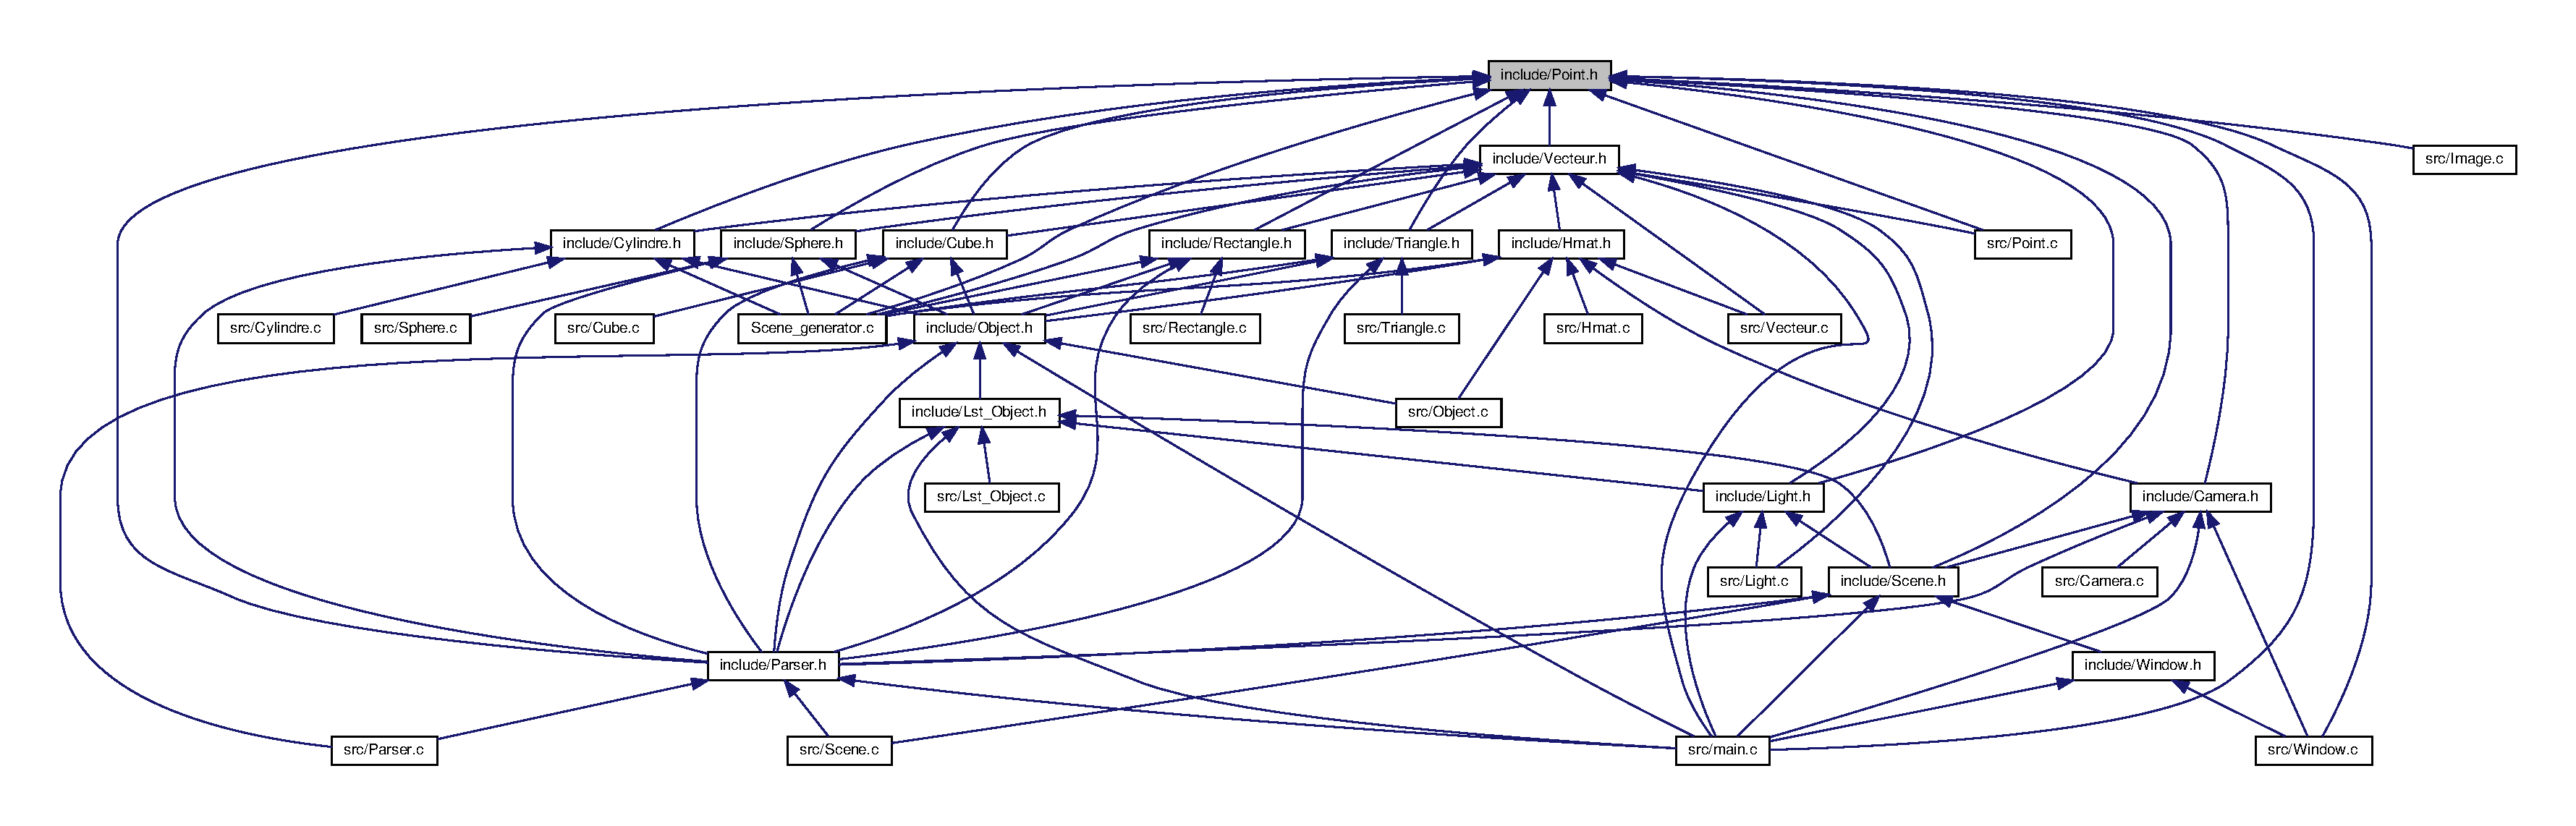
\includegraphics[width=350pt]{_point_8h__dep__incl}
\end{center}
\end{figure}
\subsection*{Data Structures}
\begin{DoxyCompactItemize}
\item 
struct \hyperlink{struct_point}{Point}
\begin{DoxyCompactList}\small\item\em a point in 3D space \end{DoxyCompactList}\end{DoxyCompactItemize}
\subsection*{Functions}
\begin{DoxyCompactItemize}
\item 
int \hyperlink{_point_8h_a23ba93e3ff33fc963b04a7a6b7d2a02e}{Point\+Copy} (\hyperlink{struct_point}{Point} $\ast$dest, const \hyperlink{struct_point}{Point} $\ast$src)
\begin{DoxyCompactList}\small\item\em copy a point to another \end{DoxyCompactList}\item 
int \hyperlink{_point_8h_ab29783f805e84cb225f1655f0193b958}{set\+Point} (\hyperlink{struct_point}{Point} $\ast$p, \hyperlink{g3x__transfo_8h_a89b2b23e407882a535d835574a7912e1}{double} x, \hyperlink{g3x__transfo_8h_a89b2b23e407882a535d835574a7912e1}{double} y, \hyperlink{g3x__transfo_8h_a89b2b23e407882a535d835574a7912e1}{double} z)
\begin{DoxyCompactList}\small\item\em sets the point with the specified values \end{DoxyCompactList}\item 
int \hyperlink{_point_8h_a8912155316eb1b59ccbc9af652fa85f5}{Point\+Center} (\hyperlink{struct_point}{Point} $\ast$res, const \hyperlink{struct_point}{Point} $\ast$A, const \hyperlink{struct_point}{Point} $\ast$B)
\begin{DoxyCompactList}\small\item\em computes the center of the segment \mbox{[}AB\mbox{]} \end{DoxyCompactList}\item 
int \hyperlink{_point_8h_ae023f752cbf662f10bb4b9086e871aa3}{Point\+Distance} (const \hyperlink{struct_point}{Point} $\ast$A, const \hyperlink{struct_point}{Point} $\ast$B, \hyperlink{g3x__transfo_8h_a89b2b23e407882a535d835574a7912e1}{double} $\ast$res)
\begin{DoxyCompactList}\small\item\em computes the distance between two points \end{DoxyCompactList}\item 
int \hyperlink{_point_8h_ab6956f8b3de44009fe28b420c4df3dbe}{Point\+Norme\+L2} (const \hyperlink{struct_point}{Point} $\ast$A, const \hyperlink{struct_point}{Point} $\ast$B, \hyperlink{g3x__transfo_8h_a89b2b23e407882a535d835574a7912e1}{double} $\ast$res)
\begin{DoxyCompactList}\small\item\em computes the maximum norm of two points \end{DoxyCompactList}\item 
int \hyperlink{_point_8h_ac811169e97b55bc567f51e34d8c85e4f}{Point\+Barycentre} (const \hyperlink{struct_point}{Point} $\ast$A, const \hyperlink{struct_point}{Point} $\ast$B, const \hyperlink{struct_point}{Point} $\ast$C, \hyperlink{struct_point}{Point} $\ast$Bary\+Centre)
\begin{DoxyCompactList}\small\item\em computes the barycenter of three points \end{DoxyCompactList}\item 
int \hyperlink{_point_8h_a9aa4b8ef9609540b0a58f4b841b2da12}{Point\+Console\+Display} (const \hyperlink{struct_point}{Point} $\ast$p, int return\+\_\+line)
\begin{DoxyCompactList}\small\item\em print a point in the console \end{DoxyCompactList}\end{DoxyCompactItemize}


\subsection{Detailed Description}
contains the \hyperlink{struct_point}{Point} type in a 3D space and all functions related to this type 

\begin{DoxyAuthor}{Author}
Jean-\/\+Manuel E\+R\+I\+A\+LC -\/ Hadjer D\+J\+E\+R\+R\+O\+U\+MI 
\end{DoxyAuthor}
\begin{DoxyVersion}{Version}
0.\+1 
\end{DoxyVersion}
\begin{DoxyDate}{Date}
11 juin 2020
\end{DoxyDate}
contains the vector type in a 3D space and all functions related to this type 

\subsection{Function Documentation}
\mbox{\Hypertarget{_point_8h_ac811169e97b55bc567f51e34d8c85e4f}\label{_point_8h_ac811169e97b55bc567f51e34d8c85e4f}} 
\index{Point.\+h@{Point.\+h}!Point\+Barycentre@{Point\+Barycentre}}
\index{Point\+Barycentre@{Point\+Barycentre}!Point.\+h@{Point.\+h}}
\subsubsection{\texorpdfstring{Point\+Barycentre()}{PointBarycentre()}}
{\footnotesize\ttfamily int Point\+Barycentre (\begin{DoxyParamCaption}\item[{const \hyperlink{struct_point}{Point} $\ast$}]{A,  }\item[{const \hyperlink{struct_point}{Point} $\ast$}]{B,  }\item[{const \hyperlink{struct_point}{Point} $\ast$}]{C,  }\item[{\hyperlink{struct_point}{Point} $\ast$}]{Bary\+Centre }\end{DoxyParamCaption})}



computes the barycenter of three points 


\begin{DoxyParams}{Parameters}
{\em A} & the first point \\
\hline
{\em B} & the second point \\
\hline
{\em C} & the third point \\
\hline
{\em Bary\+Centre} & the computed barycenter \\
\hline
\end{DoxyParams}
\begin{DoxyReturn}{Returns}
0 if a error occurs(one parameter is N\+U\+L\+L)~\newline
 1 otherwise 
\end{DoxyReturn}
\mbox{\Hypertarget{_point_8h_a8912155316eb1b59ccbc9af652fa85f5}\label{_point_8h_a8912155316eb1b59ccbc9af652fa85f5}} 
\index{Point.\+h@{Point.\+h}!Point\+Center@{Point\+Center}}
\index{Point\+Center@{Point\+Center}!Point.\+h@{Point.\+h}}
\subsubsection{\texorpdfstring{Point\+Center()}{PointCenter()}}
{\footnotesize\ttfamily int Point\+Center (\begin{DoxyParamCaption}\item[{\hyperlink{struct_point}{Point} $\ast$}]{res,  }\item[{const \hyperlink{struct_point}{Point} $\ast$}]{A,  }\item[{const \hyperlink{struct_point}{Point} $\ast$}]{B }\end{DoxyParamCaption})}



computes the center of the segment \mbox{[}AB\mbox{]} 


\begin{DoxyParams}{Parameters}
{\em res} & the result \\
\hline
{\em A} & the first point \\
\hline
{\em B} & the second point \\
\hline
\end{DoxyParams}
\begin{DoxyReturn}{Returns}
0 if a error occurs(one parameter is N\+U\+L\+L)~\newline
 1 otherwise 
\end{DoxyReturn}
\mbox{\Hypertarget{_point_8h_a9aa4b8ef9609540b0a58f4b841b2da12}\label{_point_8h_a9aa4b8ef9609540b0a58f4b841b2da12}} 
\index{Point.\+h@{Point.\+h}!Point\+Console\+Display@{Point\+Console\+Display}}
\index{Point\+Console\+Display@{Point\+Console\+Display}!Point.\+h@{Point.\+h}}
\subsubsection{\texorpdfstring{Point\+Console\+Display()}{PointConsoleDisplay()}}
{\footnotesize\ttfamily int Point\+Console\+Display (\begin{DoxyParamCaption}\item[{const \hyperlink{struct_point}{Point} $\ast$}]{p,  }\item[{int}]{return\+\_\+line }\end{DoxyParamCaption})}



print a point in the console 


\begin{DoxyParams}{Parameters}
{\em p} & the point to print \\
\hline
{\em return\+\_\+line} & != 0 if we want to add a \textquotesingle{}~\newline
\textquotesingle{} after the print \\
\hline
\end{DoxyParams}
\begin{DoxyReturn}{Returns}
0 if a error occurs(p == N\+U\+LL)~\newline
 1 otherwise 
\end{DoxyReturn}
\mbox{\Hypertarget{_point_8h_a23ba93e3ff33fc963b04a7a6b7d2a02e}\label{_point_8h_a23ba93e3ff33fc963b04a7a6b7d2a02e}} 
\index{Point.\+h@{Point.\+h}!Point\+Copy@{Point\+Copy}}
\index{Point\+Copy@{Point\+Copy}!Point.\+h@{Point.\+h}}
\subsubsection{\texorpdfstring{Point\+Copy()}{PointCopy()}}
{\footnotesize\ttfamily int Point\+Copy (\begin{DoxyParamCaption}\item[{\hyperlink{struct_point}{Point} $\ast$}]{dest,  }\item[{const \hyperlink{struct_point}{Point} $\ast$}]{src }\end{DoxyParamCaption})}



copy a point to another 


\begin{DoxyParams}{Parameters}
{\em dest} & the destination point \\
\hline
{\em src} & the point to copy \\
\hline
\end{DoxyParams}
\begin{DoxyReturn}{Returns}
0 if a error occurs(dest == N\+U\+LL $\vert$$\vert$ A == src)~\newline
 1 otherwise 
\end{DoxyReturn}
\mbox{\Hypertarget{_point_8h_ae023f752cbf662f10bb4b9086e871aa3}\label{_point_8h_ae023f752cbf662f10bb4b9086e871aa3}} 
\index{Point.\+h@{Point.\+h}!Point\+Distance@{Point\+Distance}}
\index{Point\+Distance@{Point\+Distance}!Point.\+h@{Point.\+h}}
\subsubsection{\texorpdfstring{Point\+Distance()}{PointDistance()}}
{\footnotesize\ttfamily int Point\+Distance (\begin{DoxyParamCaption}\item[{const \hyperlink{struct_point}{Point} $\ast$}]{A,  }\item[{const \hyperlink{struct_point}{Point} $\ast$}]{B,  }\item[{\hyperlink{g3x__transfo_8h_a89b2b23e407882a535d835574a7912e1}{double} $\ast$}]{res }\end{DoxyParamCaption})}



computes the distance between two points 


\begin{DoxyParams}{Parameters}
{\em A} & the first point \\
\hline
{\em B} & the second point \\
\hline
{\em res} & the result \\
\hline
\end{DoxyParams}
\begin{DoxyReturn}{Returns}
0 if a error occurs(one parameter is N\+U\+L\+L)~\newline
 1 otherwise 
\end{DoxyReturn}
\mbox{\Hypertarget{_point_8h_ab6956f8b3de44009fe28b420c4df3dbe}\label{_point_8h_ab6956f8b3de44009fe28b420c4df3dbe}} 
\index{Point.\+h@{Point.\+h}!Point\+Norme\+L2@{Point\+Norme\+L2}}
\index{Point\+Norme\+L2@{Point\+Norme\+L2}!Point.\+h@{Point.\+h}}
\subsubsection{\texorpdfstring{Point\+Norme\+L2()}{PointNormeL2()}}
{\footnotesize\ttfamily int Point\+Norme\+L2 (\begin{DoxyParamCaption}\item[{const \hyperlink{struct_point}{Point} $\ast$}]{A,  }\item[{const \hyperlink{struct_point}{Point} $\ast$}]{B,  }\item[{\hyperlink{g3x__transfo_8h_a89b2b23e407882a535d835574a7912e1}{double} $\ast$}]{res }\end{DoxyParamCaption})}



computes the maximum norm of two points 


\begin{DoxyParams}{Parameters}
{\em A} & the first point \\
\hline
{\em B} & the second point \\
\hline
{\em res} & the result \\
\hline
\end{DoxyParams}
\begin{DoxyReturn}{Returns}
0 if a error occurs(one parameter is N\+U\+L\+L)~\newline
 1 otherwise 
\end{DoxyReturn}
\mbox{\Hypertarget{_point_8h_ab29783f805e84cb225f1655f0193b958}\label{_point_8h_ab29783f805e84cb225f1655f0193b958}} 
\index{Point.\+h@{Point.\+h}!set\+Point@{set\+Point}}
\index{set\+Point@{set\+Point}!Point.\+h@{Point.\+h}}
\subsubsection{\texorpdfstring{set\+Point()}{setPoint()}}
{\footnotesize\ttfamily int set\+Point (\begin{DoxyParamCaption}\item[{\hyperlink{struct_point}{Point} $\ast$}]{p,  }\item[{\hyperlink{g3x__transfo_8h_a89b2b23e407882a535d835574a7912e1}{double}}]{x,  }\item[{\hyperlink{g3x__transfo_8h_a89b2b23e407882a535d835574a7912e1}{double}}]{y,  }\item[{\hyperlink{g3x__transfo_8h_a89b2b23e407882a535d835574a7912e1}{double}}]{z }\end{DoxyParamCaption})}



sets the point with the specified values 


\begin{DoxyParams}{Parameters}
{\em p} & the point to change \\
\hline
{\em x} & the x coordinate \\
\hline
{\em y} & the y coordinate \\
\hline
{\em z} & the z coordinate \\
\hline
\end{DoxyParams}
\begin{DoxyReturn}{Returns}
0 if a error occurs(p == N\+U\+LL)~\newline
 1 otherwise 
\end{DoxyReturn}

\hypertarget{_rectangle_8h}{}\section{include/\+Rectangle.h File Reference}
\label{_rectangle_8h}\index{include/\+Rectangle.\+h@{include/\+Rectangle.\+h}}


represents the Light type  


{\ttfamily \#include \char`\"{}Color.\+h\char`\"{}}\newline
{\ttfamily \#include \char`\"{}Point.\+h\char`\"{}}\newline
{\ttfamily \#include \char`\"{}Vecteur.\+h\char`\"{}}\newline
Include dependency graph for Rectangle.\+h\+:\nopagebreak
\begin{figure}[H]
\begin{center}
\leavevmode
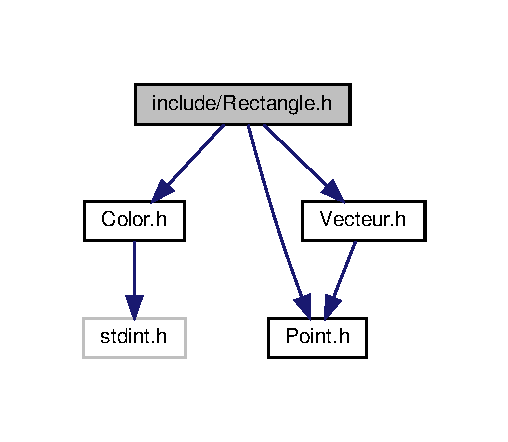
\includegraphics[width=244pt]{_rectangle_8h__incl}
\end{center}
\end{figure}
This graph shows which files directly or indirectly include this file\+:\nopagebreak
\begin{figure}[H]
\begin{center}
\leavevmode
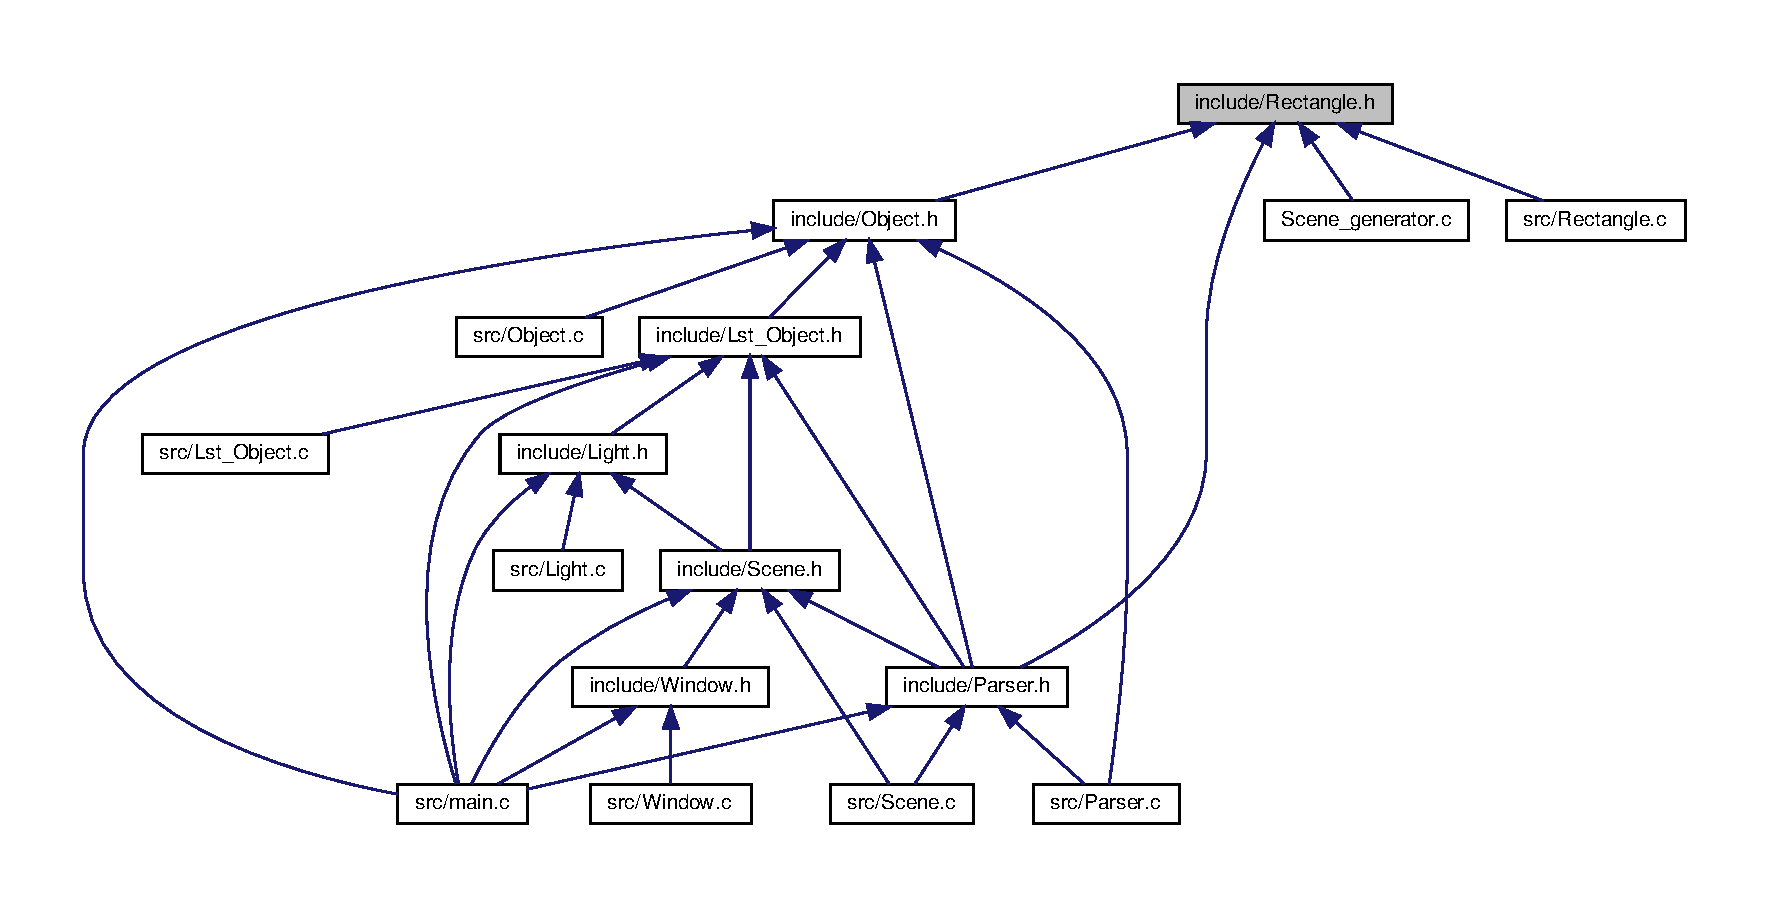
\includegraphics[width=350pt]{_rectangle_8h__dep__incl}
\end{center}
\end{figure}
\subsection*{Data Structures}
\begin{DoxyCompactItemize}
\item 
struct \hyperlink{struct_rectangle}{Rectangle}
\begin{DoxyCompactList}\small\item\em a rectangle \end{DoxyCompactList}\end{DoxyCompactItemize}
\subsection*{Functions}
\begin{DoxyCompactItemize}
\item 
int \hyperlink{_rectangle_8h_a9aff16097d4e9df9801c98fa8638dfb2}{set\+Rectangle} (\hyperlink{struct_rectangle}{Rectangle} $\ast$rectangle, const \hyperlink{struct_point}{Point} $\ast$center, const \hyperlink{struct_vecteur}{Vecteur} $\ast$u, const \hyperlink{struct_vecteur}{Vecteur} $\ast$v, \hyperlink{g3x__transfo_8h_a89b2b23e407882a535d835574a7912e1}{double} rayon, const \hyperlink{struct_color}{Color} $\ast$color)
\begin{DoxyCompactList}\small\item\em sets a rectangle with the specified parameters \end{DoxyCompactList}\item 
int \hyperlink{_rectangle_8h_aa9c2d50faa142feb4c3cc03a8c5ee1e2}{rayon\+\_\+inter\+\_\+\+Square} (const \hyperlink{struct_point}{Point} $\ast$A, const \hyperlink{struct_vecteur}{Vecteur} $\ast$u, \hyperlink{struct_point}{Point} $\ast$I, \hyperlink{struct_vecteur}{Vecteur} $\ast$N)
\begin{DoxyCompactList}\small\item\em check the intersection between a line (A, u) and the canonical square \end{DoxyCompactList}\item 
int \hyperlink{_rectangle_8h_a023ebad00750bac8b434afdcb5b48387}{Rectangle\+Console\+Display} (const \hyperlink{struct_rectangle}{Rectangle} $\ast$rectangle, int return\+\_\+line)
\begin{DoxyCompactList}\small\item\em print a rectangle in the console \end{DoxyCompactList}\end{DoxyCompactItemize}


\subsection{Detailed Description}
represents the Light type 

represents a rectangle

represents an object (shape)

\begin{DoxyAuthor}{Author}
Jean-\/\+Manuel E\+R\+I\+A\+LC -\/ Hadjer D\+J\+E\+R\+R\+O\+U\+MI 
\end{DoxyAuthor}
\begin{DoxyVersion}{Version}
0.\+1 
\end{DoxyVersion}
\begin{DoxyDate}{Date}
11 juin 2020
\end{DoxyDate}
represents the Light type in 3D space and contains functions related it

\begin{DoxyAuthor}{Author}
Jean-\/\+Manuel E\+R\+I\+A\+LC -\/ Hadjer D\+J\+E\+R\+R\+O\+U\+MI 
\end{DoxyAuthor}
\begin{DoxyVersion}{Version}
0.\+1 
\end{DoxyVersion}
\begin{DoxyDate}{Date}
11 juin 2020
\end{DoxyDate}
contains the type representing an object (shape) in a 3D space and functions related to it

\begin{DoxyAuthor}{Author}
Jean-\/\+Manuel E\+R\+I\+A\+LC -\/ Hadjer D\+J\+E\+R\+R\+O\+U\+MI 
\end{DoxyAuthor}
\begin{DoxyVersion}{Version}
0.\+1 
\end{DoxyVersion}
\begin{DoxyDate}{Date}
11 juin 2020
\end{DoxyDate}
contains the type representing a rectangle in a 3D space and functions related to it 

\subsection{Function Documentation}
\mbox{\Hypertarget{_rectangle_8h_aa9c2d50faa142feb4c3cc03a8c5ee1e2}\label{_rectangle_8h_aa9c2d50faa142feb4c3cc03a8c5ee1e2}} 
\index{Rectangle.\+h@{Rectangle.\+h}!rayon\+\_\+inter\+\_\+\+Square@{rayon\+\_\+inter\+\_\+\+Square}}
\index{rayon\+\_\+inter\+\_\+\+Square@{rayon\+\_\+inter\+\_\+\+Square}!Rectangle.\+h@{Rectangle.\+h}}
\subsubsection{\texorpdfstring{rayon\+\_\+inter\+\_\+\+Square()}{rayon\_inter\_Square()}}
{\footnotesize\ttfamily int rayon\+\_\+inter\+\_\+\+Square (\begin{DoxyParamCaption}\item[{const \hyperlink{struct_point}{Point} $\ast$}]{A,  }\item[{const \hyperlink{struct_vecteur}{Vecteur} $\ast$}]{u,  }\item[{\hyperlink{struct_point}{Point} $\ast$}]{I,  }\item[{\hyperlink{struct_vecteur}{Vecteur} $\ast$}]{N }\end{DoxyParamCaption})}



check the intersection between a line (A, u) and the canonical square 


\begin{DoxyParams}{Parameters}
{\em A} & a point of the line \\
\hline
{\em u} & the normalized director vector of the line \\
\hline
{\em I} & the intersection point if it exists \\
\hline
{\em N} & the normal vector in I \\
\hline
\end{DoxyParams}
\begin{DoxyReturn}{Returns}
0 if a error occurs(one parameter is N\+U\+L\+L)~\newline
 1 otherwise 
\end{DoxyReturn}
\mbox{\Hypertarget{_rectangle_8h_a023ebad00750bac8b434afdcb5b48387}\label{_rectangle_8h_a023ebad00750bac8b434afdcb5b48387}} 
\index{Rectangle.\+h@{Rectangle.\+h}!Rectangle\+Console\+Display@{Rectangle\+Console\+Display}}
\index{Rectangle\+Console\+Display@{Rectangle\+Console\+Display}!Rectangle.\+h@{Rectangle.\+h}}
\subsubsection{\texorpdfstring{Rectangle\+Console\+Display()}{RectangleConsoleDisplay()}}
{\footnotesize\ttfamily int Rectangle\+Console\+Display (\begin{DoxyParamCaption}\item[{const \hyperlink{struct_rectangle}{Rectangle} $\ast$}]{rectangle,  }\item[{int}]{return\+\_\+line }\end{DoxyParamCaption})}



print a rectangle in the console 


\begin{DoxyParams}{Parameters}
{\em rectangle} & the rectangle to print \\
\hline
{\em return\+\_\+line} & != 0 if we want to add a \textquotesingle{}~\newline
\textquotesingle{} after the print \\
\hline
\end{DoxyParams}
\begin{DoxyReturn}{Returns}
0 if a error occurs(rectangle == N\+U\+LL)~\newline
 1 otherwise 
\end{DoxyReturn}
\mbox{\Hypertarget{_rectangle_8h_a9aff16097d4e9df9801c98fa8638dfb2}\label{_rectangle_8h_a9aff16097d4e9df9801c98fa8638dfb2}} 
\index{Rectangle.\+h@{Rectangle.\+h}!set\+Rectangle@{set\+Rectangle}}
\index{set\+Rectangle@{set\+Rectangle}!Rectangle.\+h@{Rectangle.\+h}}
\subsubsection{\texorpdfstring{set\+Rectangle()}{setRectangle()}}
{\footnotesize\ttfamily int set\+Rectangle (\begin{DoxyParamCaption}\item[{\hyperlink{struct_rectangle}{Rectangle} $\ast$}]{rectangle,  }\item[{const \hyperlink{struct_point}{Point} $\ast$}]{center,  }\item[{const \hyperlink{struct_vecteur}{Vecteur} $\ast$}]{u,  }\item[{const \hyperlink{struct_vecteur}{Vecteur} $\ast$}]{v,  }\item[{\hyperlink{g3x__transfo_8h_a89b2b23e407882a535d835574a7912e1}{double}}]{rayon,  }\item[{const \hyperlink{struct_color}{Color} $\ast$}]{color }\end{DoxyParamCaption})}



sets a rectangle with the specified parameters 


\begin{DoxyParams}{Parameters}
{\em rectangle} & the rectangle to set \\
\hline
{\em center} & the center point \\
\hline
{\em u} & the first vector of the angle \\
\hline
{\em v} & the second vector of the angle \\
\hline
{\em rayon} & the radius \\
\hline
{\em color} & the color \\
\hline
\end{DoxyParams}
\begin{DoxyReturn}{Returns}
0 if a error occurs(one parameter is N\+U\+L\+L)~\newline
 1 otherwise 
\end{DoxyReturn}

\hypertarget{_scene_8h}{}\section{include/\+Scene.h File Reference}
\label{_scene_8h}\index{include/\+Scene.\+h@{include/\+Scene.\+h}}


represents a scene  


{\ttfamily \#include \char`\"{}Point.\+h\char`\"{}}\newline
{\ttfamily \#include \char`\"{}Camera.\+h\char`\"{}}\newline
{\ttfamily \#include \char`\"{}Image.\+h\char`\"{}}\newline
{\ttfamily \#include \char`\"{}Light.\+h\char`\"{}}\newline
{\ttfamily \#include \char`\"{}Lst\+\_\+\+Object.\+h\char`\"{}}\newline
{\ttfamily \#include \char`\"{}Option.\+h\char`\"{}}\newline
Include dependency graph for Scene.\+h\+:\nopagebreak
\begin{figure}[H]
\begin{center}
\leavevmode
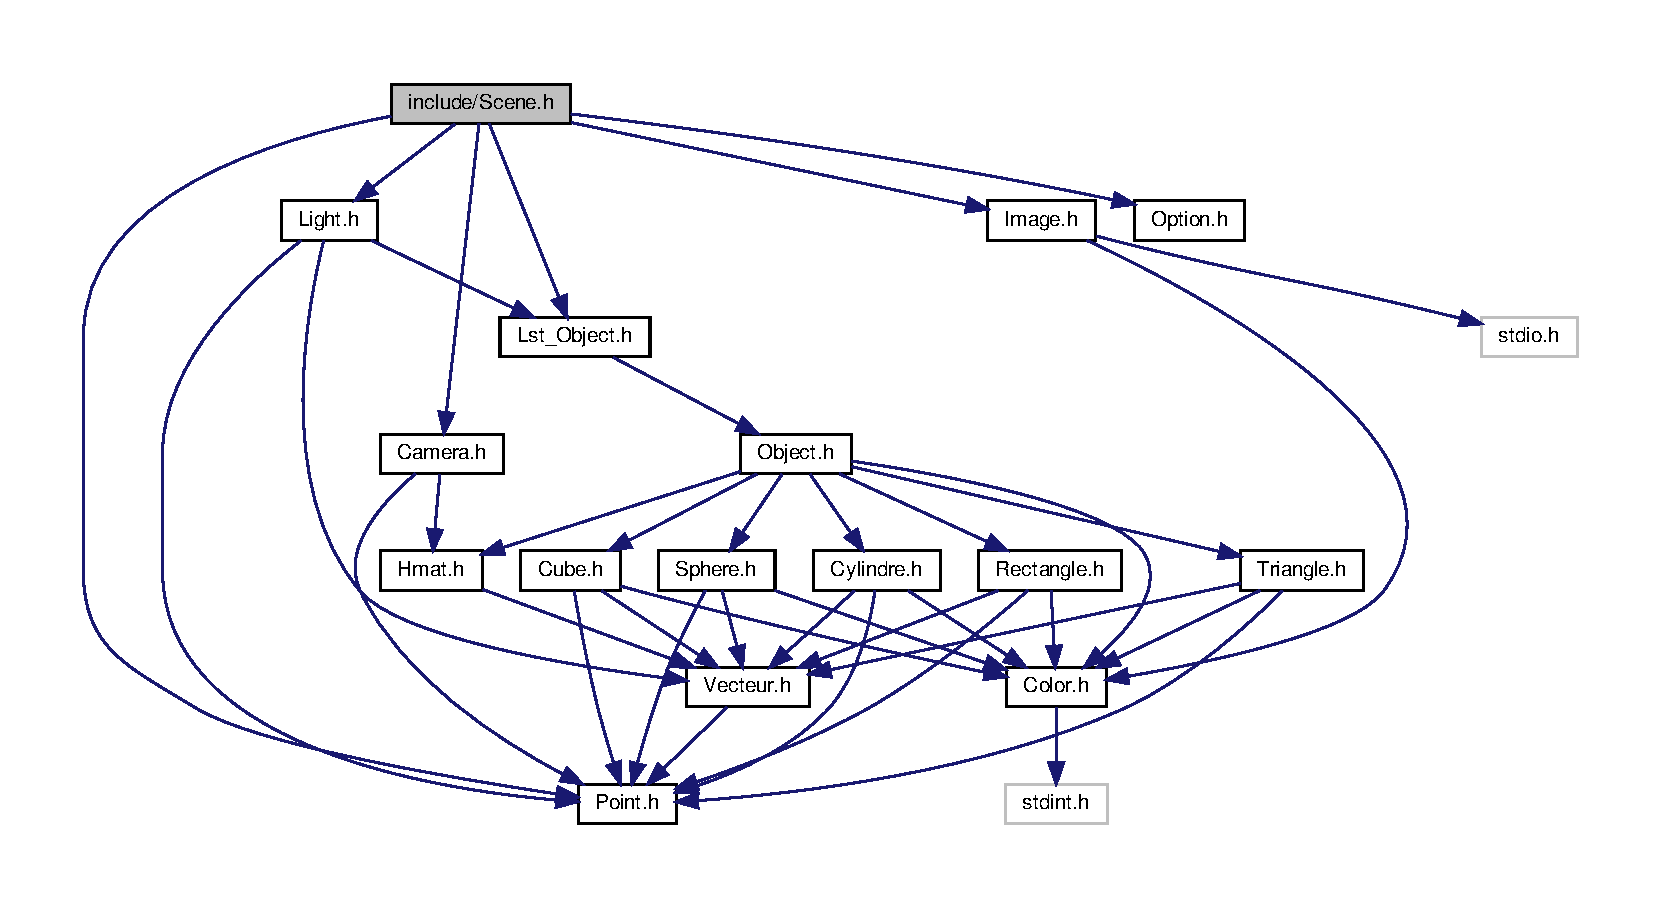
\includegraphics[width=350pt]{_scene_8h__incl}
\end{center}
\end{figure}
This graph shows which files directly or indirectly include this file\+:\nopagebreak
\begin{figure}[H]
\begin{center}
\leavevmode
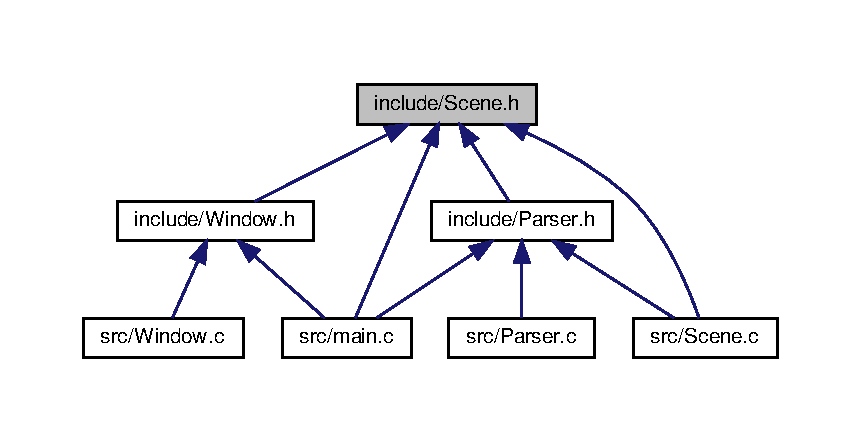
\includegraphics[width=350pt]{_scene_8h__dep__incl}
\end{center}
\end{figure}
\subsection*{Data Structures}
\begin{DoxyCompactItemize}
\item 
struct \hyperlink{struct_scene}{Scene}
\begin{DoxyCompactList}\small\item\em the 3D scene seen by the camera \end{DoxyCompactList}\end{DoxyCompactItemize}
\subsection*{Functions}
\begin{DoxyCompactItemize}
\item 
void \hyperlink{_scene_8h_af83be19419ea4b4ae9637d283c484ec8}{Scene\+\_\+init} (\hyperlink{struct_scene}{Scene} $\ast$scene)
\begin{DoxyCompactList}\small\item\em initialize an empty scene \end{DoxyCompactList}\item 
int \hyperlink{_scene_8h_a31ec65e777d0f4dd707eb039340e50c9}{create\+Scene} (\hyperlink{struct_scene}{Scene} $\ast$scene, const \hyperlink{struct_option}{Option} $\ast$options)
\begin{DoxyCompactList}\small\item\em create a scene with the specified options \end{DoxyCompactList}\item 
void \hyperlink{_scene_8h_a2f853eb65ad6d77fb89a334aecd9c5e2}{free\+Scene} (\hyperlink{struct_scene}{Scene} $\ast$scene)
\begin{DoxyCompactList}\small\item\em free all memory allocated by a scene \end{DoxyCompactList}\item 
int \hyperlink{_scene_8h_a7ecaa2f76986e0a4343b329db3bbf72a}{compute\+Scene} (\hyperlink{struct_scene}{Scene} $\ast$scene)
\begin{DoxyCompactList}\small\item\em calculate the scene and create the resulting image \end{DoxyCompactList}\item 
int \hyperlink{_scene_8h_a0767e5d6d97328d66117daea98807a31}{output\+Scene} (const \hyperlink{struct_scene}{Scene} $\ast$scene, const char $\ast$output\+\_\+file)
\begin{DoxyCompactList}\small\item\em output the computed image in a file \end{DoxyCompactList}\end{DoxyCompactItemize}


\subsection{Detailed Description}
represents a scene 

\begin{DoxyAuthor}{Author}
Jean-\/\+Manuel E\+R\+I\+A\+LC -\/ Hadjer D\+J\+E\+R\+R\+O\+U\+MI 
\end{DoxyAuthor}
\begin{DoxyVersion}{Version}
0.\+1 
\end{DoxyVersion}
\begin{DoxyDate}{Date}
11 juin 2020
\end{DoxyDate}
Contains a type \hyperlink{struct_scene}{Scene} representing a 3D scene and functions related to it. The scene can be seen via a graphic window or exported as an image. The scene contains shapes and light sources. 

\subsection{Function Documentation}
\mbox{\Hypertarget{_scene_8h_a7ecaa2f76986e0a4343b329db3bbf72a}\label{_scene_8h_a7ecaa2f76986e0a4343b329db3bbf72a}} 
\index{Scene.\+h@{Scene.\+h}!compute\+Scene@{compute\+Scene}}
\index{compute\+Scene@{compute\+Scene}!Scene.\+h@{Scene.\+h}}
\subsubsection{\texorpdfstring{compute\+Scene()}{computeScene()}}
{\footnotesize\ttfamily int compute\+Scene (\begin{DoxyParamCaption}\item[{\hyperlink{struct_scene}{Scene} $\ast$}]{scene }\end{DoxyParamCaption})}



calculate the scene and create the resulting image 


\begin{DoxyParams}{Parameters}
{\em scene} & the scene \\
\hline
\end{DoxyParams}
\begin{DoxyReturn}{Returns}
0 if a error occurs(scene == N\+U\+LL)~\newline
 1 otherwise 
\end{DoxyReturn}
\mbox{\Hypertarget{_scene_8h_a31ec65e777d0f4dd707eb039340e50c9}\label{_scene_8h_a31ec65e777d0f4dd707eb039340e50c9}} 
\index{Scene.\+h@{Scene.\+h}!create\+Scene@{create\+Scene}}
\index{create\+Scene@{create\+Scene}!Scene.\+h@{Scene.\+h}}
\subsubsection{\texorpdfstring{create\+Scene()}{createScene()}}
{\footnotesize\ttfamily int create\+Scene (\begin{DoxyParamCaption}\item[{\hyperlink{struct_scene}{Scene} $\ast$}]{scene,  }\item[{const \hyperlink{struct_option}{Option} $\ast$}]{options }\end{DoxyParamCaption})}



create a scene with the specified options 


\begin{DoxyParams}{Parameters}
{\em scene} & pointer to a scene which will contains the scene \\
\hline
{\em options} & options that the scene should respect \\
\hline
\end{DoxyParams}
\begin{DoxyReturn}{Returns}
0 if a error occurs(scene == N\+U\+LL $\vert$$\vert$ options == N\+U\+LL)~\newline
 1 otherwise 
\end{DoxyReturn}
\mbox{\Hypertarget{_scene_8h_a2f853eb65ad6d77fb89a334aecd9c5e2}\label{_scene_8h_a2f853eb65ad6d77fb89a334aecd9c5e2}} 
\index{Scene.\+h@{Scene.\+h}!free\+Scene@{free\+Scene}}
\index{free\+Scene@{free\+Scene}!Scene.\+h@{Scene.\+h}}
\subsubsection{\texorpdfstring{free\+Scene()}{freeScene()}}
{\footnotesize\ttfamily void free\+Scene (\begin{DoxyParamCaption}\item[{\hyperlink{struct_scene}{Scene} $\ast$}]{scene }\end{DoxyParamCaption})}



free all memory allocated by a scene 


\begin{DoxyParams}{Parameters}
{\em scene} & the scene we want to free \\
\hline
\end{DoxyParams}
\mbox{\Hypertarget{_scene_8h_a0767e5d6d97328d66117daea98807a31}\label{_scene_8h_a0767e5d6d97328d66117daea98807a31}} 
\index{Scene.\+h@{Scene.\+h}!output\+Scene@{output\+Scene}}
\index{output\+Scene@{output\+Scene}!Scene.\+h@{Scene.\+h}}
\subsubsection{\texorpdfstring{output\+Scene()}{outputScene()}}
{\footnotesize\ttfamily int output\+Scene (\begin{DoxyParamCaption}\item[{const \hyperlink{struct_scene}{Scene} $\ast$}]{scene,  }\item[{const char $\ast$}]{output\+\_\+file }\end{DoxyParamCaption})}



output the computed image in a file 


\begin{DoxyParams}{Parameters}
{\em scene} & the scene \\
\hline
{\em output\+\_\+file} & the file where we want to export the image \\
\hline
\end{DoxyParams}
\begin{DoxyReturn}{Returns}
0 if a error occurs(scene == N\+U\+LL $\vert$$\vert$ output\+\_\+file == N\+U\+LL or a error when writing in the file)~\newline
 1 otherwise 
\end{DoxyReturn}
\mbox{\Hypertarget{_scene_8h_af83be19419ea4b4ae9637d283c484ec8}\label{_scene_8h_af83be19419ea4b4ae9637d283c484ec8}} 
\index{Scene.\+h@{Scene.\+h}!Scene\+\_\+init@{Scene\+\_\+init}}
\index{Scene\+\_\+init@{Scene\+\_\+init}!Scene.\+h@{Scene.\+h}}
\subsubsection{\texorpdfstring{Scene\+\_\+init()}{Scene\_init()}}
{\footnotesize\ttfamily void Scene\+\_\+init (\begin{DoxyParamCaption}\item[{\hyperlink{struct_scene}{Scene} $\ast$}]{scene }\end{DoxyParamCaption})}



initialize an empty scene 


\begin{DoxyParams}{Parameters}
{\em scene} & the scene to initializ \\
\hline
\end{DoxyParams}

\hypertarget{_sphere_8h}{}\section{include/\+Sphere.h File Reference}
\label{_sphere_8h}\index{include/\+Sphere.\+h@{include/\+Sphere.\+h}}


represents a sphere  


{\ttfamily \#include \char`\"{}Color.\+h\char`\"{}}\newline
{\ttfamily \#include \char`\"{}Point.\+h\char`\"{}}\newline
{\ttfamily \#include \char`\"{}Vecteur.\+h\char`\"{}}\newline
Include dependency graph for Sphere.\+h\+:\nopagebreak
\begin{figure}[H]
\begin{center}
\leavevmode
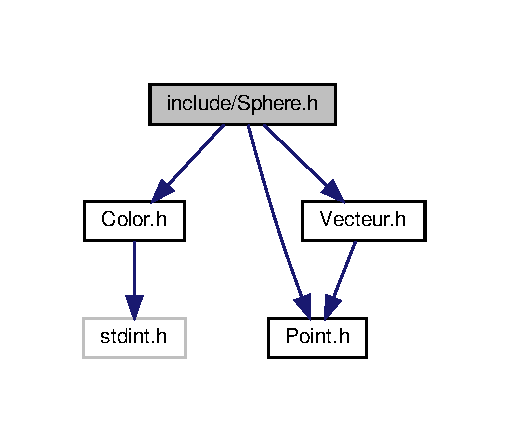
\includegraphics[width=244pt]{_sphere_8h__incl}
\end{center}
\end{figure}
This graph shows which files directly or indirectly include this file\+:\nopagebreak
\begin{figure}[H]
\begin{center}
\leavevmode
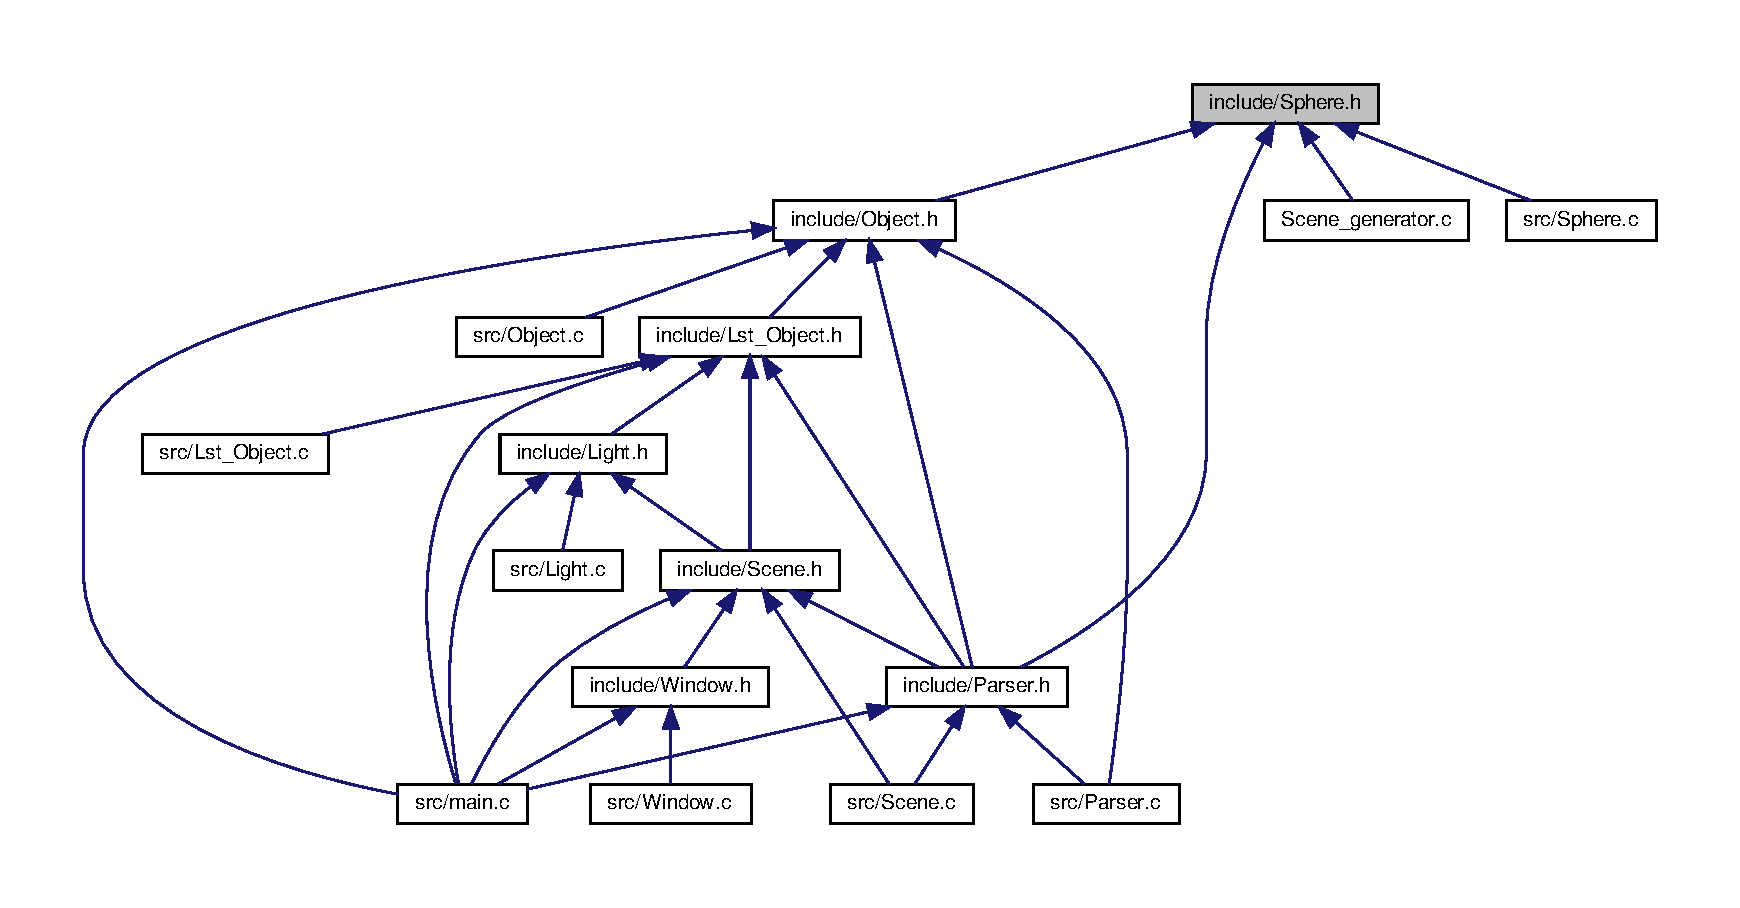
\includegraphics[width=350pt]{_sphere_8h__dep__incl}
\end{center}
\end{figure}
\subsection*{Data Structures}
\begin{DoxyCompactItemize}
\item 
struct \hyperlink{struct_sphere}{Sphere}
\begin{DoxyCompactList}\small\item\em a sphere \end{DoxyCompactList}\end{DoxyCompactItemize}
\subsection*{Functions}
\begin{DoxyCompactItemize}
\item 
int \hyperlink{_sphere_8h_a9bfa8587bf8bb481e35af44c1f04bcae}{set\+Sphere} (\hyperlink{struct_sphere}{Sphere} $\ast$sphere, const \hyperlink{struct_point}{Point} $\ast$center, const \hyperlink{struct_color}{Color} $\ast$color, \hyperlink{g3x__transfo_8h_a89b2b23e407882a535d835574a7912e1}{double} rayon)
\begin{DoxyCompactList}\small\item\em sets a sphere with the specified parameters \end{DoxyCompactList}\item 
int \hyperlink{_sphere_8h_af0c79e024b188a78f449b9dcb2524a68}{rayon\+\_\+inter\+\_\+\+Sphere} (const \hyperlink{struct_point}{Point} $\ast$A, const \hyperlink{struct_vecteur}{Vecteur} $\ast$u, \hyperlink{struct_point}{Point} $\ast$I, \hyperlink{struct_vecteur}{Vecteur} $\ast$N)
\begin{DoxyCompactList}\small\item\em check the intersection between a line (A, u) and the canonical sphere \end{DoxyCompactList}\item 
int \hyperlink{_sphere_8h_a28b4acee12968c1b12b9ee731737ba36}{Sphere\+Console\+Display} (const \hyperlink{struct_sphere}{Sphere} $\ast$sphere, int return\+\_\+line)
\begin{DoxyCompactList}\small\item\em print a sphere in the console \end{DoxyCompactList}\end{DoxyCompactItemize}


\subsection{Detailed Description}
represents a sphere 

\begin{DoxyAuthor}{Author}
Jean-\/\+Manuel E\+R\+I\+A\+LC -\/ Hadjer D\+J\+E\+R\+R\+O\+U\+MI 
\end{DoxyAuthor}
\begin{DoxyVersion}{Version}
0.\+1 
\end{DoxyVersion}
\begin{DoxyDate}{Date}
11 juin 2020
\end{DoxyDate}
contains the type representing a sphere in a 3D space and functions related to it 

\subsection{Function Documentation}
\mbox{\Hypertarget{_sphere_8h_af0c79e024b188a78f449b9dcb2524a68}\label{_sphere_8h_af0c79e024b188a78f449b9dcb2524a68}} 
\index{Sphere.\+h@{Sphere.\+h}!rayon\+\_\+inter\+\_\+\+Sphere@{rayon\+\_\+inter\+\_\+\+Sphere}}
\index{rayon\+\_\+inter\+\_\+\+Sphere@{rayon\+\_\+inter\+\_\+\+Sphere}!Sphere.\+h@{Sphere.\+h}}
\subsubsection{\texorpdfstring{rayon\+\_\+inter\+\_\+\+Sphere()}{rayon\_inter\_Sphere()}}
{\footnotesize\ttfamily int rayon\+\_\+inter\+\_\+\+Sphere (\begin{DoxyParamCaption}\item[{const \hyperlink{struct_point}{Point} $\ast$}]{A,  }\item[{const \hyperlink{struct_vecteur}{Vecteur} $\ast$}]{u,  }\item[{\hyperlink{struct_point}{Point} $\ast$}]{I,  }\item[{\hyperlink{struct_vecteur}{Vecteur} $\ast$}]{N }\end{DoxyParamCaption})}



check the intersection between a line (A, u) and the canonical sphere 


\begin{DoxyParams}{Parameters}
{\em A} & a point of the line \\
\hline
{\em u} & the normalized director vector of the line \\
\hline
{\em I} & the intersection point if it exists \\
\hline
{\em N} & the normal vector in I \\
\hline
\end{DoxyParams}
\begin{DoxyReturn}{Returns}
0 if a error occurs(one parameter is N\+U\+L\+L)~\newline
 1 otherwise 
\end{DoxyReturn}
\mbox{\Hypertarget{_sphere_8h_a9bfa8587bf8bb481e35af44c1f04bcae}\label{_sphere_8h_a9bfa8587bf8bb481e35af44c1f04bcae}} 
\index{Sphere.\+h@{Sphere.\+h}!set\+Sphere@{set\+Sphere}}
\index{set\+Sphere@{set\+Sphere}!Sphere.\+h@{Sphere.\+h}}
\subsubsection{\texorpdfstring{set\+Sphere()}{setSphere()}}
{\footnotesize\ttfamily int set\+Sphere (\begin{DoxyParamCaption}\item[{\hyperlink{struct_sphere}{Sphere} $\ast$}]{sphere,  }\item[{const \hyperlink{struct_point}{Point} $\ast$}]{center,  }\item[{const \hyperlink{struct_color}{Color} $\ast$}]{color,  }\item[{\hyperlink{g3x__transfo_8h_a89b2b23e407882a535d835574a7912e1}{double}}]{rayon }\end{DoxyParamCaption})}



sets a sphere with the specified parameters 


\begin{DoxyParams}{Parameters}
{\em sphere} & the sphere to set \\
\hline
{\em center} & ther new center \\
\hline
{\em color} & the new color \\
\hline
{\em rayon} & the new radius \\
\hline
\end{DoxyParams}
\begin{DoxyReturn}{Returns}
0 if a error occurs(one parameter is N\+U\+L\+L)~\newline
 1 otherwise 
\end{DoxyReturn}
\mbox{\Hypertarget{_sphere_8h_a28b4acee12968c1b12b9ee731737ba36}\label{_sphere_8h_a28b4acee12968c1b12b9ee731737ba36}} 
\index{Sphere.\+h@{Sphere.\+h}!Sphere\+Console\+Display@{Sphere\+Console\+Display}}
\index{Sphere\+Console\+Display@{Sphere\+Console\+Display}!Sphere.\+h@{Sphere.\+h}}
\subsubsection{\texorpdfstring{Sphere\+Console\+Display()}{SphereConsoleDisplay()}}
{\footnotesize\ttfamily int Sphere\+Console\+Display (\begin{DoxyParamCaption}\item[{const \hyperlink{struct_sphere}{Sphere} $\ast$}]{sphere,  }\item[{int}]{return\+\_\+line }\end{DoxyParamCaption})}



print a sphere in the console 


\begin{DoxyParams}{Parameters}
{\em sphere} & the sphere to print \\
\hline
{\em return\+\_\+line} & != 0 if we want to add a \textquotesingle{}~\newline
\textquotesingle{} after the print \\
\hline
\end{DoxyParams}
\begin{DoxyReturn}{Returns}
0 if a error occurs(sphere == N\+U\+LL)~\newline
 1 otherwise 
\end{DoxyReturn}

\hypertarget{_triangle_8h}{}\section{include/\+Triangle.h File Reference}
\label{_triangle_8h}\index{include/\+Triangle.\+h@{include/\+Triangle.\+h}}


represents a triangle  


{\ttfamily \#include \char`\"{}Color.\+h\char`\"{}}\newline
{\ttfamily \#include \char`\"{}Point.\+h\char`\"{}}\newline
{\ttfamily \#include \char`\"{}Vecteur.\+h\char`\"{}}\newline
Include dependency graph for Triangle.\+h\+:\nopagebreak
\begin{figure}[H]
\begin{center}
\leavevmode
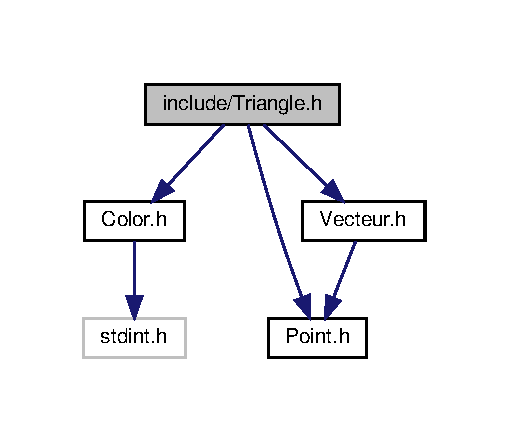
\includegraphics[width=244pt]{_triangle_8h__incl}
\end{center}
\end{figure}
This graph shows which files directly or indirectly include this file\+:\nopagebreak
\begin{figure}[H]
\begin{center}
\leavevmode
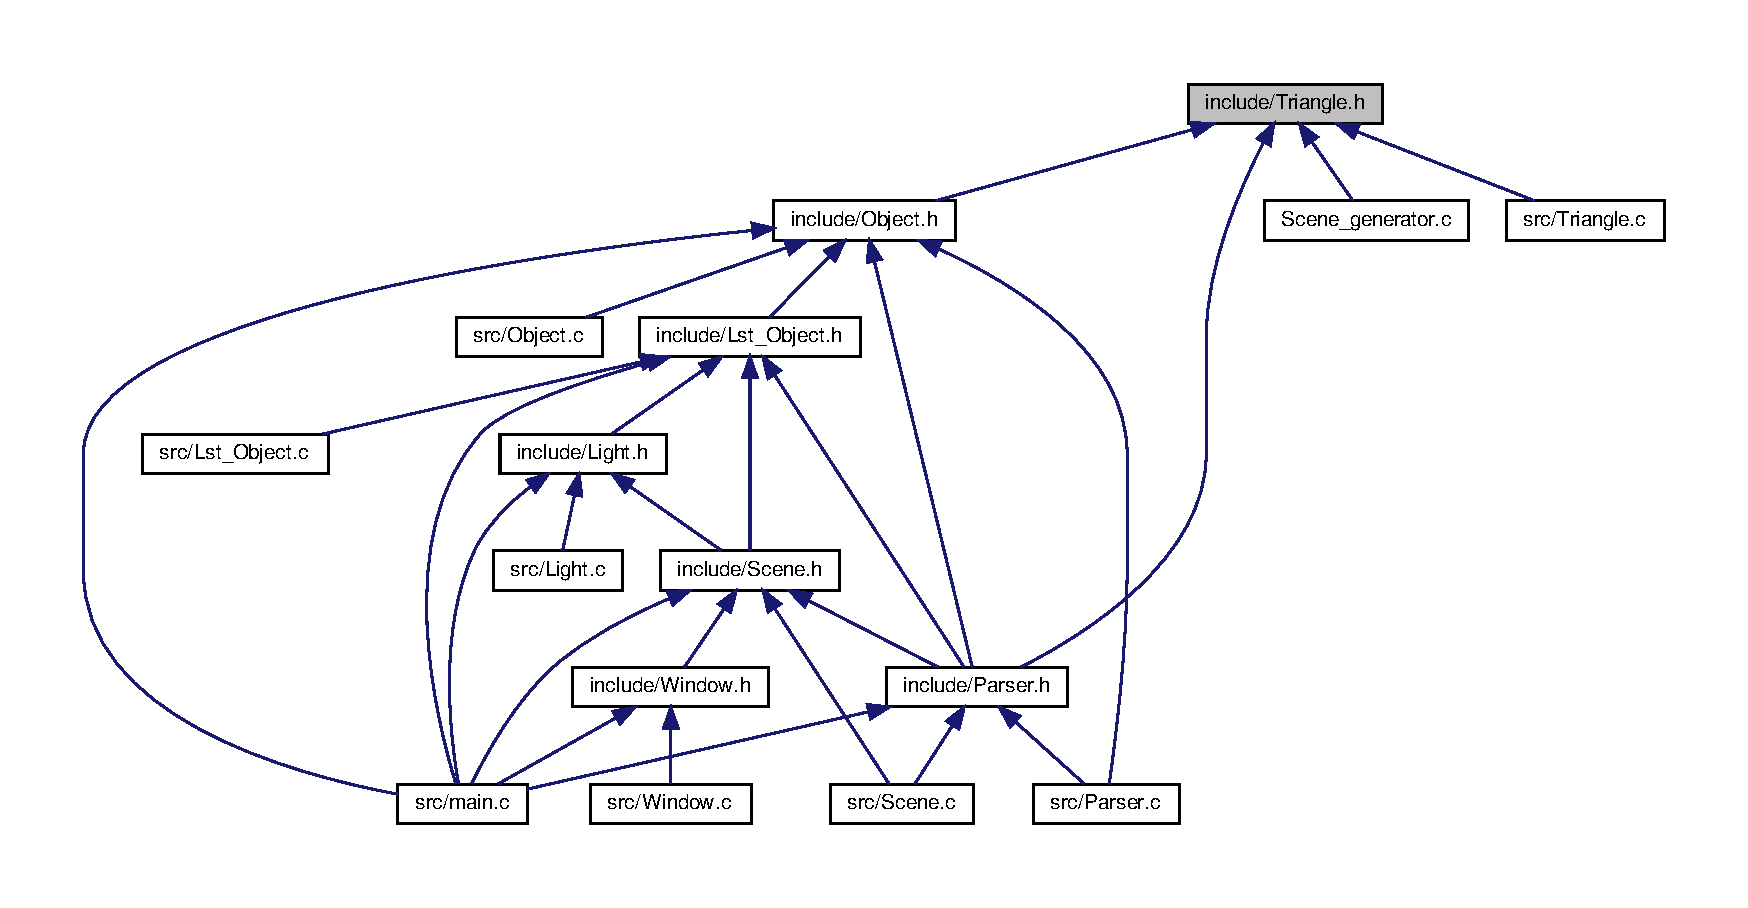
\includegraphics[width=350pt]{_triangle_8h__dep__incl}
\end{center}
\end{figure}
\subsection*{Data Structures}
\begin{DoxyCompactItemize}
\item 
struct \hyperlink{struct_triangle}{Triangle}
\begin{DoxyCompactList}\small\item\em a triangle \end{DoxyCompactList}\end{DoxyCompactItemize}
\subsection*{Functions}
\begin{DoxyCompactItemize}
\item 
int \hyperlink{_triangle_8h_ad04bb458fe3bd495e998082db022e975}{set\+Triangle} (\hyperlink{struct_triangle}{Triangle} $\ast$triangle, const \hyperlink{struct_point}{Point} $\ast$A, const \hyperlink{struct_point}{Point} $\ast$B, const \hyperlink{struct_point}{Point} $\ast$C, const \hyperlink{struct_color}{Color} $\ast$color)
\begin{DoxyCompactList}\small\item\em sets a triangle with new parameters \end{DoxyCompactList}\item 
int \hyperlink{_triangle_8h_afbcc4f6858457479194ddfac0ce1e9be}{rayon\+\_\+inter\+\_\+\+Triangle} (const \hyperlink{struct_point}{Point} $\ast$A, const \hyperlink{struct_vecteur}{Vecteur} $\ast$u, \hyperlink{struct_point}{Point} $\ast$I, \hyperlink{struct_vecteur}{Vecteur} $\ast$N)
\begin{DoxyCompactList}\small\item\em check the intersection between a line (A, u) and the canonical triangle \end{DoxyCompactList}\item 
int \hyperlink{_triangle_8h_aafa4aca3401af14f8bd7b2b5ca0b9045}{Triangle\+Point\+In\+Triangle} (const \hyperlink{struct_point}{Point} $\ast$A, const \hyperlink{struct_point}{Point} $\ast$B, const \hyperlink{struct_point}{Point} $\ast$C, const \hyperlink{struct_point}{Point} $\ast$I)
\begin{DoxyCompactList}\small\item\em check if the triangle (A\+BC) contains the point I \end{DoxyCompactList}\item 
int \hyperlink{_triangle_8h_a490ef09eece5b69adde9c82ce25a5db0}{Triangle\+Console\+Display} (const \hyperlink{struct_triangle}{Triangle} $\ast$triangle, int return\+\_\+line)
\begin{DoxyCompactList}\small\item\em print a triangle in the console \end{DoxyCompactList}\end{DoxyCompactItemize}


\subsection{Detailed Description}
represents a triangle 

\begin{DoxyAuthor}{Author}
Jean-\/\+Manuel E\+R\+I\+A\+LC -\/ Hadjer D\+J\+E\+R\+R\+O\+U\+MI 
\end{DoxyAuthor}
\begin{DoxyVersion}{Version}
0.\+1 
\end{DoxyVersion}
\begin{DoxyDate}{Date}
11 juin 2020
\end{DoxyDate}
contains the type representing a triangle in a 3D space and functions related to it 

\subsection{Function Documentation}
\mbox{\Hypertarget{_triangle_8h_afbcc4f6858457479194ddfac0ce1e9be}\label{_triangle_8h_afbcc4f6858457479194ddfac0ce1e9be}} 
\index{Triangle.\+h@{Triangle.\+h}!rayon\+\_\+inter\+\_\+\+Triangle@{rayon\+\_\+inter\+\_\+\+Triangle}}
\index{rayon\+\_\+inter\+\_\+\+Triangle@{rayon\+\_\+inter\+\_\+\+Triangle}!Triangle.\+h@{Triangle.\+h}}
\subsubsection{\texorpdfstring{rayon\+\_\+inter\+\_\+\+Triangle()}{rayon\_inter\_Triangle()}}
{\footnotesize\ttfamily int rayon\+\_\+inter\+\_\+\+Triangle (\begin{DoxyParamCaption}\item[{const \hyperlink{struct_point}{Point} $\ast$}]{A,  }\item[{const \hyperlink{struct_vecteur}{Vecteur} $\ast$}]{u,  }\item[{\hyperlink{struct_point}{Point} $\ast$}]{I,  }\item[{\hyperlink{struct_vecteur}{Vecteur} $\ast$}]{N }\end{DoxyParamCaption})}



check the intersection between a line (A, u) and the canonical triangle 


\begin{DoxyParams}{Parameters}
{\em A} & a point of the line \\
\hline
{\em u} & the normalized director vector of the line \\
\hline
{\em I} & the intersection point if it exists \\
\hline
{\em N} & the normal vector in I \\
\hline
\end{DoxyParams}
\begin{DoxyReturn}{Returns}
0 if a error occurs(one parameter is N\+U\+L\+L)~\newline
 1 otherwise 
\end{DoxyReturn}
\mbox{\Hypertarget{_triangle_8h_ad04bb458fe3bd495e998082db022e975}\label{_triangle_8h_ad04bb458fe3bd495e998082db022e975}} 
\index{Triangle.\+h@{Triangle.\+h}!set\+Triangle@{set\+Triangle}}
\index{set\+Triangle@{set\+Triangle}!Triangle.\+h@{Triangle.\+h}}
\subsubsection{\texorpdfstring{set\+Triangle()}{setTriangle()}}
{\footnotesize\ttfamily int set\+Triangle (\begin{DoxyParamCaption}\item[{\hyperlink{struct_triangle}{Triangle} $\ast$}]{triangle,  }\item[{const \hyperlink{struct_point}{Point} $\ast$}]{A,  }\item[{const \hyperlink{struct_point}{Point} $\ast$}]{B,  }\item[{const \hyperlink{struct_point}{Point} $\ast$}]{C,  }\item[{const \hyperlink{struct_color}{Color} $\ast$}]{color }\end{DoxyParamCaption})}



sets a triangle with new parameters 


\begin{DoxyParams}{Parameters}
{\em triangle} & the triangle to set \\
\hline
{\em A} & the first point \\
\hline
{\em B} & the second point \\
\hline
{\em C} & the third point \\
\hline
{\em color} & the color \\
\hline
\end{DoxyParams}
\begin{DoxyReturn}{Returns}
0 if a error occurs(one parameter is N\+U\+L\+L)~\newline
 1 otherwise 
\end{DoxyReturn}
\mbox{\Hypertarget{_triangle_8h_a490ef09eece5b69adde9c82ce25a5db0}\label{_triangle_8h_a490ef09eece5b69adde9c82ce25a5db0}} 
\index{Triangle.\+h@{Triangle.\+h}!Triangle\+Console\+Display@{Triangle\+Console\+Display}}
\index{Triangle\+Console\+Display@{Triangle\+Console\+Display}!Triangle.\+h@{Triangle.\+h}}
\subsubsection{\texorpdfstring{Triangle\+Console\+Display()}{TriangleConsoleDisplay()}}
{\footnotesize\ttfamily int int Triangle\+Console\+Display (\begin{DoxyParamCaption}\item[{const \hyperlink{struct_triangle}{Triangle} $\ast$}]{triangle,  }\item[{int}]{return\+\_\+line }\end{DoxyParamCaption})}



print a triangle in the console 


\begin{DoxyParams}{Parameters}
{\em triangle} & the triangle to print \\
\hline
{\em return\+\_\+line} & != 0 if we want to add a \textquotesingle{}~\newline
\textquotesingle{} after the print \\
\hline
\end{DoxyParams}
\begin{DoxyReturn}{Returns}
0 if a error occurs(triangle == N\+U\+LL)~\newline
 1 otherwise 
\end{DoxyReturn}
\mbox{\Hypertarget{_triangle_8h_aafa4aca3401af14f8bd7b2b5ca0b9045}\label{_triangle_8h_aafa4aca3401af14f8bd7b2b5ca0b9045}} 
\index{Triangle.\+h@{Triangle.\+h}!Triangle\+Point\+In\+Triangle@{Triangle\+Point\+In\+Triangle}}
\index{Triangle\+Point\+In\+Triangle@{Triangle\+Point\+In\+Triangle}!Triangle.\+h@{Triangle.\+h}}
\subsubsection{\texorpdfstring{Triangle\+Point\+In\+Triangle()}{TrianglePointInTriangle()}}
{\footnotesize\ttfamily int Triangle\+Point\+In\+Triangle (\begin{DoxyParamCaption}\item[{const \hyperlink{struct_point}{Point} $\ast$}]{A,  }\item[{const \hyperlink{struct_point}{Point} $\ast$}]{B,  }\item[{const \hyperlink{struct_point}{Point} $\ast$}]{C,  }\item[{const \hyperlink{struct_point}{Point} $\ast$}]{I }\end{DoxyParamCaption})}



check if the triangle (A\+BC) contains the point I 


\begin{DoxyParams}{Parameters}
{\em A} & the first point of the triangle \\
\hline
{\em B} & the second point of the triangle \\
\hline
{\em C} & the third point of the triangle \\
\hline
{\em I} & a point \\
\hline
\end{DoxyParams}
\begin{DoxyReturn}{Returns}
-\/1 if a error occurs(one parameter is N\+U\+L\+L)~\newline
 0 if the triangle contains I~\newline
 1 otherwise 
\end{DoxyReturn}

\hypertarget{_vecteur_8h}{}\section{include/\+Vecteur.h File Reference}
\label{_vecteur_8h}\index{include/\+Vecteur.\+h@{include/\+Vecteur.\+h}}


contains the vector type in a 3D space and all functions related to this type  


{\ttfamily \#include \char`\"{}Point.\+h\char`\"{}}\newline
Include dependency graph for Vecteur.\+h\+:\nopagebreak
\begin{figure}[H]
\begin{center}
\leavevmode
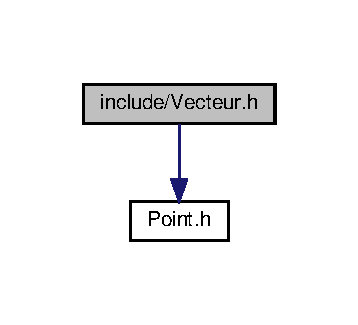
\includegraphics[width=172pt]{_vecteur_8h__incl}
\end{center}
\end{figure}
This graph shows which files directly or indirectly include this file\+:\nopagebreak
\begin{figure}[H]
\begin{center}
\leavevmode
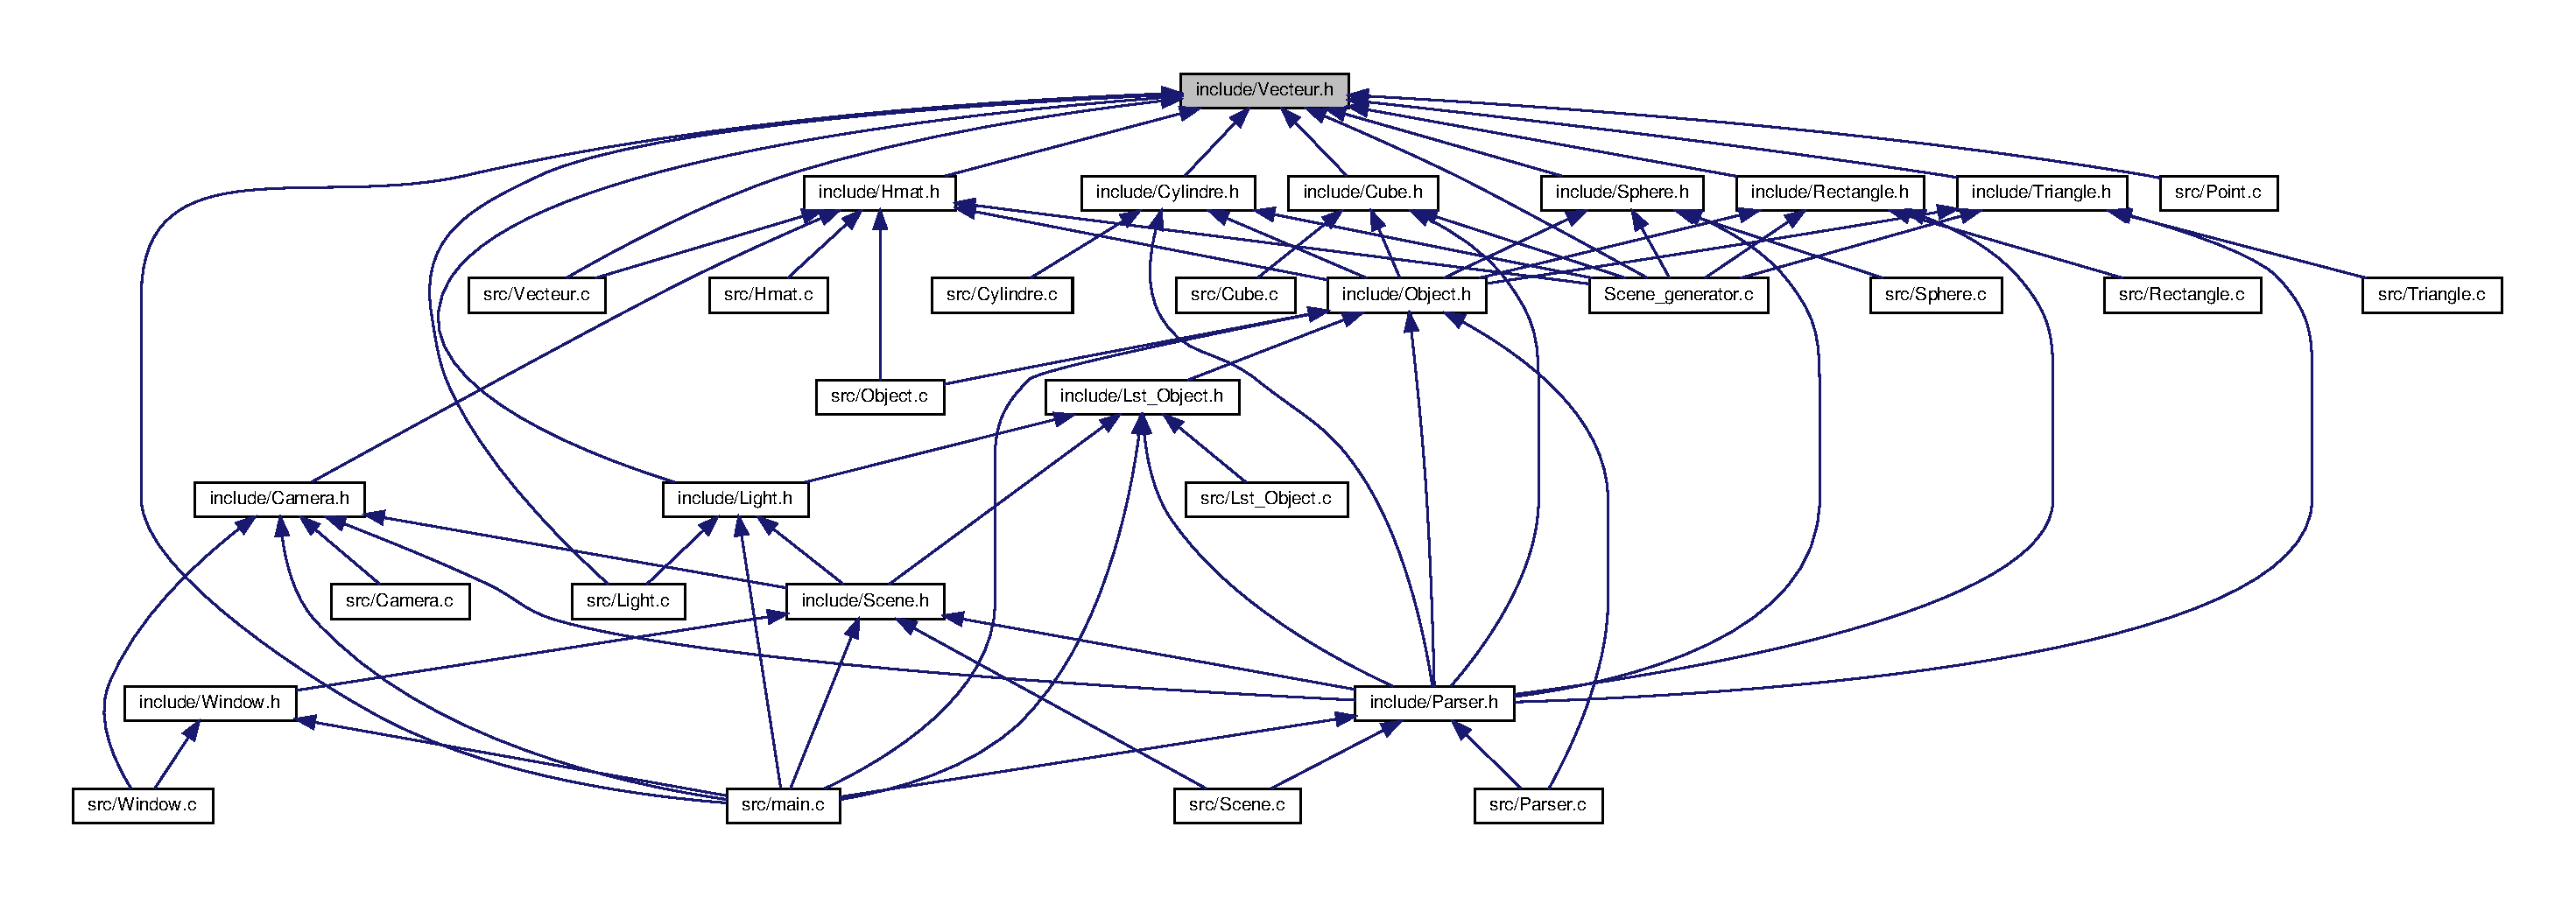
\includegraphics[width=350pt]{_vecteur_8h__dep__incl}
\end{center}
\end{figure}
\subsection*{Data Structures}
\begin{DoxyCompactItemize}
\item 
struct \hyperlink{struct_vecteur}{Vecteur}
\begin{DoxyCompactList}\small\item\em represents a vector in 3D space. \end{DoxyCompactList}\end{DoxyCompactItemize}
\subsection*{Functions}
\begin{DoxyCompactItemize}
\item 
int \hyperlink{_vecteur_8h_a4db9ffb37e52a22f9a901d0ba616192c}{Vecteur\+Of\+Points} (\hyperlink{struct_vecteur}{Vecteur} $\ast$vecteur, const \hyperlink{struct_point}{Point} $\ast$A, const \hyperlink{struct_point}{Point} $\ast$B)
\begin{DoxyCompactList}\small\item\em compute the vector passing through points A and B \end{DoxyCompactList}\item 
int \hyperlink{_vecteur_8h_ab5f0ea47eec7035820dc636bc61bf80f}{Vecteur\+Copy} (\hyperlink{struct_vecteur}{Vecteur} $\ast$dest, const \hyperlink{struct_vecteur}{Vecteur} $\ast$src)
\begin{DoxyCompactList}\small\item\em copy a vector to another \end{DoxyCompactList}\item 
int \hyperlink{_vecteur_8h_adf999ed64bdebe4b762a638fbe49cc65}{set\+Vecteur} (\hyperlink{struct_vecteur}{Vecteur} $\ast$u, \hyperlink{g3x__transfo_8h_a89b2b23e407882a535d835574a7912e1}{double} x, \hyperlink{g3x__transfo_8h_a89b2b23e407882a535d835574a7912e1}{double} y, \hyperlink{g3x__transfo_8h_a89b2b23e407882a535d835574a7912e1}{double} z)
\begin{DoxyCompactList}\small\item\em sets the vector with the specified values \end{DoxyCompactList}\item 
int \hyperlink{_vecteur_8h_a091c0a1eb8d2f71463d20916f870ae11}{Vecteur\+Normalize} (\hyperlink{struct_vecteur}{Vecteur} $\ast$u)
\begin{DoxyCompactList}\small\item\em normalizes a vector \end{DoxyCompactList}\item 
int \hyperlink{_vecteur_8h_af72d3969977142380c84e05b0361c66a}{Vecteur\+Square\+Norme} (const \hyperlink{struct_vecteur}{Vecteur} $\ast$u, \hyperlink{g3x__transfo_8h_a89b2b23e407882a535d835574a7912e1}{double} $\ast$res)
\begin{DoxyCompactList}\small\item\em get the square of the norm of a vector \end{DoxyCompactList}\item 
int \hyperlink{_vecteur_8h_a8bb7fb8516b57380aac7736579cd9682}{Vecteur\+Prod\+\_\+scal} (const \hyperlink{struct_vecteur}{Vecteur} $\ast$u, const \hyperlink{struct_vecteur}{Vecteur} $\ast$v, \hyperlink{g3x__transfo_8h_a89b2b23e407882a535d835574a7912e1}{double} $\ast$res)
\begin{DoxyCompactList}\small\item\em computes the dot product of two vectors \end{DoxyCompactList}\item 
int \hyperlink{_vecteur_8h_a01197256fb34963d4b9fc485f3a4052e}{Vecteur\+Prod\+\_\+vec} (const \hyperlink{struct_vecteur}{Vecteur} $\ast$u, const \hyperlink{struct_vecteur}{Vecteur} $\ast$v, \hyperlink{struct_vecteur}{Vecteur} $\ast$new\+Vecteur)
\begin{DoxyCompactList}\small\item\em computes the vector product of two vectors \end{DoxyCompactList}\item 
int \hyperlink{_vecteur_8h_ab9bb35c984b458d5f9d6cd7050dece93}{Sinus} (const \hyperlink{struct_vecteur}{Vecteur} $\ast$u, const \hyperlink{struct_vecteur}{Vecteur} $\ast$v, \hyperlink{g3x__transfo_8h_a89b2b23e407882a535d835574a7912e1}{double} $\ast$res)
\begin{DoxyCompactList}\small\item\em compute the sine of an angle(u, v) \end{DoxyCompactList}\item 
int \hyperlink{_vecteur_8h_acd17e01734456773119bf807b243a3d3}{Cosinus} (const \hyperlink{struct_vecteur}{Vecteur} $\ast$u, const \hyperlink{struct_vecteur}{Vecteur} $\ast$v, \hyperlink{g3x__transfo_8h_a89b2b23e407882a535d835574a7912e1}{double} $\ast$res)
\begin{DoxyCompactList}\small\item\em compute the cosine of an angle(u, v) \end{DoxyCompactList}\item 
int \hyperlink{_vecteur_8h_a86862e27cb0ba6c33f438a51cf8a0db1}{Vecteur\+Equals} (const \hyperlink{struct_vecteur}{Vecteur} $\ast$u, const \hyperlink{struct_vecteur}{Vecteur} $\ast$v)
\begin{DoxyCompactList}\small\item\em tells if a vector is equal to another \end{DoxyCompactList}\item 
int \hyperlink{_vecteur_8h_a7f02ea0460266fbf202c014c3140fa67}{Vecteur\+Is\+Zero} (const \hyperlink{struct_vecteur}{Vecteur} $\ast$u)
\begin{DoxyCompactList}\small\item\em check if the norme of a vector is zero \end{DoxyCompactList}\item 
int \hyperlink{_vecteur_8h_a9ff68ff8eedb91cfa80a040b9d7718a0}{Vecteur\+Angles\+Equals} (\hyperlink{struct_vecteur}{Vecteur} $\ast$u1, \hyperlink{struct_vecteur}{Vecteur} $\ast$u2, \hyperlink{struct_vecteur}{Vecteur} $\ast$v1, \hyperlink{struct_vecteur}{Vecteur} $\ast$v2)
\begin{DoxyCompactList}\small\item\em check if tow angles are equals \end{DoxyCompactList}\item 
int \hyperlink{_vecteur_8h_a91b8b94ba3cfdf7676f02bb8bc3c8969}{Vecteur\+Half} (const \hyperlink{struct_vecteur}{Vecteur} $\ast$u, const \hyperlink{struct_vecteur}{Vecteur} $\ast$v, \hyperlink{struct_vecteur}{Vecteur} $\ast$res)
\begin{DoxyCompactList}\small\item\em calculates the half vector of two vectors \end{DoxyCompactList}\item 
int \hyperlink{_vecteur_8h_a3729c85facb0a4adf098a6286786d2a6}{Vecteur\+Reflected} (const \hyperlink{struct_vecteur}{Vecteur} $\ast$u, const \hyperlink{struct_vecteur}{Vecteur} $\ast$N, \hyperlink{struct_vecteur}{Vecteur} $\ast$res)
\begin{DoxyCompactList}\small\item\em sets the vector with the specified values \end{DoxyCompactList}\item 
int \hyperlink{_vecteur_8h_a07297e041358d184cf258e2f2289a35b}{Vecteur\+Console\+Display} (const \hyperlink{struct_vecteur}{Vecteur} $\ast$vecteur, int return\+\_\+line)
\begin{DoxyCompactList}\small\item\em print a vector in the console \end{DoxyCompactList}\end{DoxyCompactItemize}


\subsection{Detailed Description}
contains the vector type in a 3D space and all functions related to this type 

\begin{DoxyAuthor}{Author}
Jean-\/\+Manuel E\+R\+I\+A\+LC -\/ Hadjer D\+J\+E\+R\+R\+O\+U\+MI 
\end{DoxyAuthor}
\begin{DoxyVersion}{Version}
0.\+1 
\end{DoxyVersion}
\begin{DoxyDate}{Date}
11 juin 2020
\end{DoxyDate}
contains the vector type in a 3D space and all functions related to vectors and angels 

\subsection{Function Documentation}
\mbox{\Hypertarget{_vecteur_8h_acd17e01734456773119bf807b243a3d3}\label{_vecteur_8h_acd17e01734456773119bf807b243a3d3}} 
\index{Vecteur.\+h@{Vecteur.\+h}!Cosinus@{Cosinus}}
\index{Cosinus@{Cosinus}!Vecteur.\+h@{Vecteur.\+h}}
\subsubsection{\texorpdfstring{Cosinus()}{Cosinus()}}
{\footnotesize\ttfamily int Cosinus (\begin{DoxyParamCaption}\item[{const \hyperlink{struct_vecteur}{Vecteur} $\ast$}]{u,  }\item[{const \hyperlink{struct_vecteur}{Vecteur} $\ast$}]{v,  }\item[{\hyperlink{g3x__transfo_8h_a89b2b23e407882a535d835574a7912e1}{double} $\ast$}]{res }\end{DoxyParamCaption})}



compute the cosine of an angle(u, v) 


\begin{DoxyParams}{Parameters}
{\em u} & the first vector \\
\hline
{\em v} & the second vector \\
\hline
{\em res} & the computed result \\
\hline
\end{DoxyParams}
\begin{DoxyReturn}{Returns}
0 if an error occurs~\newline
 1 otherwise 
\end{DoxyReturn}
\mbox{\Hypertarget{_vecteur_8h_adf999ed64bdebe4b762a638fbe49cc65}\label{_vecteur_8h_adf999ed64bdebe4b762a638fbe49cc65}} 
\index{Vecteur.\+h@{Vecteur.\+h}!set\+Vecteur@{set\+Vecteur}}
\index{set\+Vecteur@{set\+Vecteur}!Vecteur.\+h@{Vecteur.\+h}}
\subsubsection{\texorpdfstring{set\+Vecteur()}{setVecteur()}}
{\footnotesize\ttfamily int set\+Vecteur (\begin{DoxyParamCaption}\item[{\hyperlink{struct_vecteur}{Vecteur} $\ast$}]{u,  }\item[{\hyperlink{g3x__transfo_8h_a89b2b23e407882a535d835574a7912e1}{double}}]{x,  }\item[{\hyperlink{g3x__transfo_8h_a89b2b23e407882a535d835574a7912e1}{double}}]{y,  }\item[{\hyperlink{g3x__transfo_8h_a89b2b23e407882a535d835574a7912e1}{double}}]{z }\end{DoxyParamCaption})}



sets the vector with the specified values 


\begin{DoxyParams}{Parameters}
{\em u} & the vector to change \\
\hline
{\em x} & the x coordinate \\
\hline
{\em y} & the y coordinate \\
\hline
{\em z} & the z coordinate \\
\hline
\end{DoxyParams}
\begin{DoxyReturn}{Returns}
0 if a error occurs(u == N\+U\+LL)~\newline
 1 otherwise 
\end{DoxyReturn}
\mbox{\Hypertarget{_vecteur_8h_ab9bb35c984b458d5f9d6cd7050dece93}\label{_vecteur_8h_ab9bb35c984b458d5f9d6cd7050dece93}} 
\index{Vecteur.\+h@{Vecteur.\+h}!Sinus@{Sinus}}
\index{Sinus@{Sinus}!Vecteur.\+h@{Vecteur.\+h}}
\subsubsection{\texorpdfstring{Sinus()}{Sinus()}}
{\footnotesize\ttfamily int Sinus (\begin{DoxyParamCaption}\item[{const \hyperlink{struct_vecteur}{Vecteur} $\ast$}]{u,  }\item[{const \hyperlink{struct_vecteur}{Vecteur} $\ast$}]{v,  }\item[{\hyperlink{g3x__transfo_8h_a89b2b23e407882a535d835574a7912e1}{double} $\ast$}]{res }\end{DoxyParamCaption})}



compute the sine of an angle(u, v) 


\begin{DoxyParams}{Parameters}
{\em u} & the first vector \\
\hline
{\em v} & the second vector \\
\hline
{\em res} & the computed result\\
\hline
\end{DoxyParams}
\begin{DoxyReturn}{Returns}
0 if an error occurs~\newline
 1 otherwise 
\end{DoxyReturn}
\mbox{\Hypertarget{_vecteur_8h_a9ff68ff8eedb91cfa80a040b9d7718a0}\label{_vecteur_8h_a9ff68ff8eedb91cfa80a040b9d7718a0}} 
\index{Vecteur.\+h@{Vecteur.\+h}!Vecteur\+Angles\+Equals@{Vecteur\+Angles\+Equals}}
\index{Vecteur\+Angles\+Equals@{Vecteur\+Angles\+Equals}!Vecteur.\+h@{Vecteur.\+h}}
\subsubsection{\texorpdfstring{Vecteur\+Angles\+Equals()}{VecteurAnglesEquals()}}
{\footnotesize\ttfamily int Vecteur\+Angles\+Equals (\begin{DoxyParamCaption}\item[{\hyperlink{struct_vecteur}{Vecteur} $\ast$}]{u1,  }\item[{\hyperlink{struct_vecteur}{Vecteur} $\ast$}]{u2,  }\item[{\hyperlink{struct_vecteur}{Vecteur} $\ast$}]{v1,  }\item[{\hyperlink{struct_vecteur}{Vecteur} $\ast$}]{v2 }\end{DoxyParamCaption})}



check if tow angles are equals 


\begin{DoxyParams}{Parameters}
{\em u1} & the first vector of the first angle \\
\hline
{\em u2} & the second vector of the first angle \\
\hline
{\em v1} & the first vector of the second angle \\
\hline
{\em v2} & the second vector of the second angle \\
\hline
\end{DoxyParams}
\begin{DoxyReturn}{Returns}
0 if a error occurs(one parameter is N\+U\+L\+L)~\newline
 1 otherwise 
\end{DoxyReturn}
\mbox{\Hypertarget{_vecteur_8h_a07297e041358d184cf258e2f2289a35b}\label{_vecteur_8h_a07297e041358d184cf258e2f2289a35b}} 
\index{Vecteur.\+h@{Vecteur.\+h}!Vecteur\+Console\+Display@{Vecteur\+Console\+Display}}
\index{Vecteur\+Console\+Display@{Vecteur\+Console\+Display}!Vecteur.\+h@{Vecteur.\+h}}
\subsubsection{\texorpdfstring{Vecteur\+Console\+Display()}{VecteurConsoleDisplay()}}
{\footnotesize\ttfamily int Vecteur\+Console\+Display (\begin{DoxyParamCaption}\item[{const \hyperlink{struct_vecteur}{Vecteur} $\ast$}]{vecteur,  }\item[{int}]{return\+\_\+line }\end{DoxyParamCaption})}



print a vector in the console 


\begin{DoxyParams}{Parameters}
{\em vecteur} & the vector to print \\
\hline
{\em return\+\_\+line} & != 0 if we want to add a \textquotesingle{}~\newline
\textquotesingle{} after the print \\
\hline
\end{DoxyParams}
\begin{DoxyReturn}{Returns}
0 if a error occurs(u == N\+U\+LL)~\newline
 1 otherwise 
\end{DoxyReturn}
\mbox{\Hypertarget{_vecteur_8h_ab5f0ea47eec7035820dc636bc61bf80f}\label{_vecteur_8h_ab5f0ea47eec7035820dc636bc61bf80f}} 
\index{Vecteur.\+h@{Vecteur.\+h}!Vecteur\+Copy@{Vecteur\+Copy}}
\index{Vecteur\+Copy@{Vecteur\+Copy}!Vecteur.\+h@{Vecteur.\+h}}
\subsubsection{\texorpdfstring{Vecteur\+Copy()}{VecteurCopy()}}
{\footnotesize\ttfamily int Vecteur\+Copy (\begin{DoxyParamCaption}\item[{\hyperlink{struct_vecteur}{Vecteur} $\ast$}]{dest,  }\item[{const \hyperlink{struct_vecteur}{Vecteur} $\ast$}]{src }\end{DoxyParamCaption})}



copy a vector to another 


\begin{DoxyParams}{Parameters}
{\em dest} & the vector receiving this vector \\
\hline
{\em src} & the vector to copy \\
\hline
\end{DoxyParams}
\begin{DoxyReturn}{Returns}
0 if a error occurs(dest == N\+U\+LL $\vert$$\vert$ A == src)~\newline
 1 otherwise 
\end{DoxyReturn}
\mbox{\Hypertarget{_vecteur_8h_a86862e27cb0ba6c33f438a51cf8a0db1}\label{_vecteur_8h_a86862e27cb0ba6c33f438a51cf8a0db1}} 
\index{Vecteur.\+h@{Vecteur.\+h}!Vecteur\+Equals@{Vecteur\+Equals}}
\index{Vecteur\+Equals@{Vecteur\+Equals}!Vecteur.\+h@{Vecteur.\+h}}
\subsubsection{\texorpdfstring{Vecteur\+Equals()}{VecteurEquals()}}
{\footnotesize\ttfamily int Vecteur\+Equals (\begin{DoxyParamCaption}\item[{const \hyperlink{struct_vecteur}{Vecteur} $\ast$}]{u,  }\item[{const \hyperlink{struct_vecteur}{Vecteur} $\ast$}]{v }\end{DoxyParamCaption})}



tells if a vector is equal to another 


\begin{DoxyParams}{Parameters}
{\em u} & the first vector \\
\hline
{\em v} & the second vector\\
\hline
\end{DoxyParams}
\begin{DoxyReturn}{Returns}
-\/1 if one of the vector is N\+U\+LL~\newline
 0 if the two vectors was not equals~\newline
 1 if the two vectors was equals 
\end{DoxyReturn}
\mbox{\Hypertarget{_vecteur_8h_a91b8b94ba3cfdf7676f02bb8bc3c8969}\label{_vecteur_8h_a91b8b94ba3cfdf7676f02bb8bc3c8969}} 
\index{Vecteur.\+h@{Vecteur.\+h}!Vecteur\+Half@{Vecteur\+Half}}
\index{Vecteur\+Half@{Vecteur\+Half}!Vecteur.\+h@{Vecteur.\+h}}
\subsubsection{\texorpdfstring{Vecteur\+Half()}{VecteurHalf()}}
{\footnotesize\ttfamily int Vecteur\+Half (\begin{DoxyParamCaption}\item[{const \hyperlink{struct_vecteur}{Vecteur} $\ast$}]{u,  }\item[{const \hyperlink{struct_vecteur}{Vecteur} $\ast$}]{v,  }\item[{\hyperlink{struct_vecteur}{Vecteur} $\ast$}]{res }\end{DoxyParamCaption})}



calculates the half vector of two vectors 


\begin{DoxyParams}{Parameters}
{\em u} & the first vector \\
\hline
{\em v} & the second vector \\
\hline
{\em res} & the result \\
\hline
\end{DoxyParams}
\begin{DoxyReturn}{Returns}
0 if a error occurs(u == N\+U\+LL $\vert$$\vert$ v == N\+U\+LL $\vert$$\vert$ res == N\+U\+LL)~\newline
 1 otherwise 
\end{DoxyReturn}
\mbox{\Hypertarget{_vecteur_8h_a7f02ea0460266fbf202c014c3140fa67}\label{_vecteur_8h_a7f02ea0460266fbf202c014c3140fa67}} 
\index{Vecteur.\+h@{Vecteur.\+h}!Vecteur\+Is\+Zero@{Vecteur\+Is\+Zero}}
\index{Vecteur\+Is\+Zero@{Vecteur\+Is\+Zero}!Vecteur.\+h@{Vecteur.\+h}}
\subsubsection{\texorpdfstring{Vecteur\+Is\+Zero()}{VecteurIsZero()}}
{\footnotesize\ttfamily int Vecteur\+Is\+Zero (\begin{DoxyParamCaption}\item[{const \hyperlink{struct_vecteur}{Vecteur} $\ast$}]{u }\end{DoxyParamCaption})}



check if the norme of a vector is zero 


\begin{DoxyParams}{Parameters}
{\em u} & a vector \\
\hline
\end{DoxyParams}
\begin{DoxyReturn}{Returns}
0 if a error occurs(u == N\+U\+LL)~\newline
 1 otherwise 
\end{DoxyReturn}
\mbox{\Hypertarget{_vecteur_8h_a091c0a1eb8d2f71463d20916f870ae11}\label{_vecteur_8h_a091c0a1eb8d2f71463d20916f870ae11}} 
\index{Vecteur.\+h@{Vecteur.\+h}!Vecteur\+Normalize@{Vecteur\+Normalize}}
\index{Vecteur\+Normalize@{Vecteur\+Normalize}!Vecteur.\+h@{Vecteur.\+h}}
\subsubsection{\texorpdfstring{Vecteur\+Normalize()}{VecteurNormalize()}}
{\footnotesize\ttfamily int Vecteur\+Normalize (\begin{DoxyParamCaption}\item[{\hyperlink{struct_vecteur}{Vecteur} $\ast$}]{u }\end{DoxyParamCaption})}



normalizes a vector 


\begin{DoxyParams}{Parameters}
{\em u} & the vector to normalize \\
\hline
\end{DoxyParams}
\begin{DoxyReturn}{Returns}
0 if a error occurs(u == N\+U\+LL)~\newline
 1 otherwise 
\end{DoxyReturn}
\mbox{\Hypertarget{_vecteur_8h_a4db9ffb37e52a22f9a901d0ba616192c}\label{_vecteur_8h_a4db9ffb37e52a22f9a901d0ba616192c}} 
\index{Vecteur.\+h@{Vecteur.\+h}!Vecteur\+Of\+Points@{Vecteur\+Of\+Points}}
\index{Vecteur\+Of\+Points@{Vecteur\+Of\+Points}!Vecteur.\+h@{Vecteur.\+h}}
\subsubsection{\texorpdfstring{Vecteur\+Of\+Points()}{VecteurOfPoints()}}
{\footnotesize\ttfamily int Vecteur\+Of\+Points (\begin{DoxyParamCaption}\item[{\hyperlink{struct_vecteur}{Vecteur} $\ast$}]{vecteur,  }\item[{const \hyperlink{struct_point}{Point} $\ast$}]{A,  }\item[{const \hyperlink{struct_point}{Point} $\ast$}]{B }\end{DoxyParamCaption})}



compute the vector passing through points A and B 


\begin{DoxyParams}{Parameters}
{\em vecteur} & the computed vector \\
\hline
{\em A} & \hyperlink{struct_point}{Point} A the point A \\
\hline
{\em B} & \hyperlink{struct_point}{Point} B the point B \\
\hline
\end{DoxyParams}
\begin{DoxyReturn}{Returns}
0 if a error occurs(vecteur == N\+U\+LL $\vert$$\vert$ A == N\+U\+LL $\vert$$\vert$ B == N\+U\+LL)~\newline
 1 otherwise 
\end{DoxyReturn}
\mbox{\Hypertarget{_vecteur_8h_a8bb7fb8516b57380aac7736579cd9682}\label{_vecteur_8h_a8bb7fb8516b57380aac7736579cd9682}} 
\index{Vecteur.\+h@{Vecteur.\+h}!Vecteur\+Prod\+\_\+scal@{Vecteur\+Prod\+\_\+scal}}
\index{Vecteur\+Prod\+\_\+scal@{Vecteur\+Prod\+\_\+scal}!Vecteur.\+h@{Vecteur.\+h}}
\subsubsection{\texorpdfstring{Vecteur\+Prod\+\_\+scal()}{VecteurProd\_scal()}}
{\footnotesize\ttfamily int Vecteur\+Prod\+\_\+scal (\begin{DoxyParamCaption}\item[{const \hyperlink{struct_vecteur}{Vecteur} $\ast$}]{u,  }\item[{const \hyperlink{struct_vecteur}{Vecteur} $\ast$}]{v,  }\item[{\hyperlink{g3x__transfo_8h_a89b2b23e407882a535d835574a7912e1}{double} $\ast$}]{res }\end{DoxyParamCaption})}



computes the dot product of two vectors 


\begin{DoxyParams}{Parameters}
{\em u} & the first vector \\
\hline
{\em v} & the second vector \\
\hline
{\em res} & the computed value (the dot product of u v) \\
\hline
\end{DoxyParams}
\begin{DoxyReturn}{Returns}
0 if a error occurs(u == N\+U\+LL $\vert$$\vert$ v == N\+U\+LL $\vert$$\vert$ res == N\+U\+LL)~\newline
 1 otherwise 
\end{DoxyReturn}
\mbox{\Hypertarget{_vecteur_8h_a01197256fb34963d4b9fc485f3a4052e}\label{_vecteur_8h_a01197256fb34963d4b9fc485f3a4052e}} 
\index{Vecteur.\+h@{Vecteur.\+h}!Vecteur\+Prod\+\_\+vec@{Vecteur\+Prod\+\_\+vec}}
\index{Vecteur\+Prod\+\_\+vec@{Vecteur\+Prod\+\_\+vec}!Vecteur.\+h@{Vecteur.\+h}}
\subsubsection{\texorpdfstring{Vecteur\+Prod\+\_\+vec()}{VecteurProd\_vec()}}
{\footnotesize\ttfamily int Vecteur\+Prod\+\_\+vec (\begin{DoxyParamCaption}\item[{const \hyperlink{struct_vecteur}{Vecteur} $\ast$}]{u,  }\item[{const \hyperlink{struct_vecteur}{Vecteur} $\ast$}]{v,  }\item[{\hyperlink{struct_vecteur}{Vecteur} $\ast$}]{new\+Vecteur }\end{DoxyParamCaption})}



computes the vector product of two vectors 


\begin{DoxyParams}{Parameters}
{\em u} & the first vector \\
\hline
{\em v} & the second vector \\
\hline
{\em new\+Vecteur} & the computed vector (the vector product of u v) \\
\hline
\end{DoxyParams}
\begin{DoxyReturn}{Returns}
0 if a error occurs(u == N\+U\+LL $\vert$$\vert$ v == N\+U\+LL $\vert$$\vert$ new\+Vecteur == N\+U\+LL)~\newline
 1 otherwise 
\end{DoxyReturn}
\mbox{\Hypertarget{_vecteur_8h_a3729c85facb0a4adf098a6286786d2a6}\label{_vecteur_8h_a3729c85facb0a4adf098a6286786d2a6}} 
\index{Vecteur.\+h@{Vecteur.\+h}!Vecteur\+Reflected@{Vecteur\+Reflected}}
\index{Vecteur\+Reflected@{Vecteur\+Reflected}!Vecteur.\+h@{Vecteur.\+h}}
\subsubsection{\texorpdfstring{Vecteur\+Reflected()}{VecteurReflected()}}
{\footnotesize\ttfamily int Vecteur\+Reflected (\begin{DoxyParamCaption}\item[{const \hyperlink{struct_vecteur}{Vecteur} $\ast$}]{u,  }\item[{const \hyperlink{struct_vecteur}{Vecteur} $\ast$}]{N,  }\item[{\hyperlink{struct_vecteur}{Vecteur} $\ast$}]{res }\end{DoxyParamCaption})}



sets the vector with the specified values 


\begin{DoxyParams}{Parameters}
{\em u} & the incident vector \\
\hline
{\em N} & the normal vector \\
\hline
{\em res} & the normalized reflected vector \\
\hline
\end{DoxyParams}
\begin{DoxyReturn}{Returns}
0 if a error occurs(u == N\+U\+LL $\vert$$\vert$ N == N\+U\+LL $\vert$$\vert$ res == N\+U\+LL)~\newline
 1 otherwise 
\end{DoxyReturn}
\mbox{\Hypertarget{_vecteur_8h_af72d3969977142380c84e05b0361c66a}\label{_vecteur_8h_af72d3969977142380c84e05b0361c66a}} 
\index{Vecteur.\+h@{Vecteur.\+h}!Vecteur\+Square\+Norme@{Vecteur\+Square\+Norme}}
\index{Vecteur\+Square\+Norme@{Vecteur\+Square\+Norme}!Vecteur.\+h@{Vecteur.\+h}}
\subsubsection{\texorpdfstring{Vecteur\+Square\+Norme()}{VecteurSquareNorme()}}
{\footnotesize\ttfamily int Vecteur\+Square\+Norme (\begin{DoxyParamCaption}\item[{const \hyperlink{struct_vecteur}{Vecteur} $\ast$}]{u,  }\item[{\hyperlink{g3x__transfo_8h_a89b2b23e407882a535d835574a7912e1}{double} $\ast$}]{res }\end{DoxyParamCaption})}



get the square of the norm of a vector 


\begin{DoxyParams}{Parameters}
{\em u} & the vector to change \\
\hline
{\em res} & the result \\
\hline
\end{DoxyParams}
\begin{DoxyReturn}{Returns}
0 if a error occurs(u == N\+U\+LL $\vert$$\vert$ res == N\+U\+LL)~\newline
 1 otherwise 
\end{DoxyReturn}

\hypertarget{_window_8h}{}\section{include/\+Window.h File Reference}
\label{_window_8h}\index{include/\+Window.\+h@{include/\+Window.\+h}}


represents a window to display a scene  


{\ttfamily \#include \char`\"{}Scene.\+h\char`\"{}}\newline
{\ttfamily \#include \char`\"{}Option.\+h\char`\"{}}\newline
Include dependency graph for Window.\+h\+:\nopagebreak
\begin{figure}[H]
\begin{center}
\leavevmode
\includegraphics[width=350pt]{_window_8h__incl}
\end{center}
\end{figure}
This graph shows which files directly or indirectly include this file\+:\nopagebreak
\begin{figure}[H]
\begin{center}
\leavevmode
\includegraphics[width=238pt]{_window_8h__dep__incl}
\end{center}
\end{figure}
\subsection*{Functions}
\begin{DoxyCompactItemize}
\item 
void \hyperlink{_window_8h_ad16d1568a7f9e9c2cf490bd4dfb7a293}{open\+Window} (\hyperlink{struct_scene}{Scene} $\ast$scene, \hyperlink{struct_option}{Option} $\ast$options)
\begin{DoxyCompactList}\small\item\em create a window to display a scene \end{DoxyCompactList}\end{DoxyCompactItemize}


\subsection{Detailed Description}
represents a window to display a scene 

\begin{DoxyAuthor}{Author}
Jean-\/\+Manuel E\+R\+I\+A\+LC -\/ Hadjer D\+J\+E\+R\+R\+O\+U\+MI 
\end{DoxyAuthor}
\begin{DoxyVersion}{Version}
0.\+1 
\end{DoxyVersion}
\begin{DoxyDate}{Date}
11 juin 2020
\end{DoxyDate}
represents a window to display a scene 

\subsection{Function Documentation}
\mbox{\Hypertarget{_window_8h_ad16d1568a7f9e9c2cf490bd4dfb7a293}\label{_window_8h_ad16d1568a7f9e9c2cf490bd4dfb7a293}} 
\index{Window.\+h@{Window.\+h}!open\+Window@{open\+Window}}
\index{open\+Window@{open\+Window}!Window.\+h@{Window.\+h}}
\subsubsection{\texorpdfstring{open\+Window()}{openWindow()}}
{\footnotesize\ttfamily void open\+Window (\begin{DoxyParamCaption}\item[{\hyperlink{struct_scene}{Scene} $\ast$}]{scene,  }\item[{\hyperlink{struct_option}{Option} $\ast$}]{options }\end{DoxyParamCaption})}



create a window to display a scene 


\begin{DoxyParams}{Parameters}
{\em scene} & the scene to display \\
\hline
{\em options} & the parameters specified by the user\\
\hline
\end{DoxyParams}
create a window to display a scene 
\hypertarget{g3x_8h}{}\section{libg3x/include/g3x.h File Reference}
\label{g3x_8h}\index{libg3x/include/g3x.\+h@{libg3x/include/g3x.\+h}}
{\ttfamily \#include $<$stdio.\+h$>$}\newline
{\ttfamily \#include $<$stdlib.\+h$>$}\newline
{\ttfamily \#include $<$string.\+h$>$}\newline
{\ttfamily \#include $<$math.\+h$>$}\newline
{\ttfamily \#include $<$unistd.\+h$>$}\newline
{\ttfamily \#include $<$G\+L/gl.\+h$>$}\newline
{\ttfamily \#include $<$G\+L/glut.\+h$>$}\newline
{\ttfamily \#include $<$g3x\+\_\+types.\+h$>$}\newline
{\ttfamily \#include $<$g3x\+\_\+macros.\+h$>$}\newline
{\ttfamily \#include $<$g3x\+\_\+tools.\+h$>$}\newline
{\ttfamily \#include $<$g3x\+\_\+colors.\+h$>$}\newline
{\ttfamily \#include $<$g3x\+\_\+capture.\+h$>$}\newline
{\ttfamily \#include $<$g3x\+\_\+transfo.\+h$>$}\newline
{\ttfamily \#include $<$g3x\+\_\+\+G\+Ltransfo.\+h$>$}\newline
{\ttfamily \#include $<$g3x\+\_\+quaternions.\+h$>$}\newline
{\ttfamily \#include $<$g3x\+\_\+pnm.\+h$>$}\newline
{\ttfamily \#include $<$g3x\+\_\+window.\+h$>$}\newline
Include dependency graph for g3x.\+h\+:\nopagebreak
\begin{figure}[H]
\begin{center}
\leavevmode
\includegraphics[width=350pt]{g3x_8h__incl}
\end{center}
\end{figure}
This graph shows which files directly or indirectly include this file\+:\nopagebreak
\begin{figure}[H]
\begin{center}
\leavevmode
\includegraphics[width=350pt]{g3x_8h__dep__incl}
\end{center}
\end{figure}
\subsection*{Macros}
\begin{DoxyCompactItemize}
\item 
\#define \hyperlink{g3x_8h_a369266c24eacffb87046522897a570d5}{\+\_\+\+G\+N\+U\+\_\+\+S\+O\+U\+R\+CE}
\item 
\#define \hyperlink{g3x_8h_a7d30ef058866ddaf44e496b711fdd7a2}{\+\_\+\+G3\+X\+\_\+\+H\+\_\+}
\end{DoxyCompactItemize}


\subsection{Macro Definition Documentation}
\mbox{\Hypertarget{g3x_8h_a7d30ef058866ddaf44e496b711fdd7a2}\label{g3x_8h_a7d30ef058866ddaf44e496b711fdd7a2}} 
\index{g3x.\+h@{g3x.\+h}!\+\_\+\+G3\+X\+\_\+\+H\+\_\+@{\+\_\+\+G3\+X\+\_\+\+H\+\_\+}}
\index{\+\_\+\+G3\+X\+\_\+\+H\+\_\+@{\+\_\+\+G3\+X\+\_\+\+H\+\_\+}!g3x.\+h@{g3x.\+h}}
\subsubsection{\texorpdfstring{\+\_\+\+G3\+X\+\_\+\+H\+\_\+}{\_G3X\_H\_}}
{\footnotesize\ttfamily \#define \+\_\+\+G3\+X\+\_\+\+H\+\_\+}

\mbox{\Hypertarget{g3x_8h_a369266c24eacffb87046522897a570d5}\label{g3x_8h_a369266c24eacffb87046522897a570d5}} 
\index{g3x.\+h@{g3x.\+h}!\+\_\+\+G\+N\+U\+\_\+\+S\+O\+U\+R\+CE@{\+\_\+\+G\+N\+U\+\_\+\+S\+O\+U\+R\+CE}}
\index{\+\_\+\+G\+N\+U\+\_\+\+S\+O\+U\+R\+CE@{\+\_\+\+G\+N\+U\+\_\+\+S\+O\+U\+R\+CE}!g3x.\+h@{g3x.\+h}}
\subsubsection{\texorpdfstring{\+\_\+\+G\+N\+U\+\_\+\+S\+O\+U\+R\+CE}{\_GNU\_SOURCE}}
{\footnotesize\ttfamily \#define \+\_\+\+G\+N\+U\+\_\+\+S\+O\+U\+R\+CE}


\hypertarget{g3x__capture_8h}{}\section{libg3x/include/g3x\+\_\+capture.h File Reference}
\label{g3x__capture_8h}\index{libg3x/include/g3x\+\_\+capture.\+h@{libg3x/include/g3x\+\_\+capture.\+h}}
{\ttfamily \#include $<$g3x\+\_\+types.\+h$>$}\newline
Include dependency graph for g3x\+\_\+capture.\+h\+:\nopagebreak
\begin{figure}[H]
\begin{center}
\leavevmode
\includegraphics[width=175pt]{g3x__capture_8h__incl}
\end{center}
\end{figure}
This graph shows which files directly or indirectly include this file\+:\nopagebreak
\begin{figure}[H]
\begin{center}
\leavevmode
\includegraphics[width=350pt]{g3x__capture_8h__dep__incl}
\end{center}
\end{figure}
\subsection*{Macros}
\begin{DoxyCompactItemize}
\item 
\#define \hyperlink{g3x__capture_8h_a369266c24eacffb87046522897a570d5}{\+\_\+\+G\+N\+U\+\_\+\+S\+O\+U\+R\+CE}
\item 
\#define \hyperlink{g3x__capture_8h_a2674e44f5b375f939b46cf70c832aa74}{\+\_\+\+G3\+X\+\_\+\+C\+A\+P\+T\+U\+R\+E\+\_\+}
\end{DoxyCompactItemize}
\subsection*{Functions}
\begin{DoxyCompactItemize}
\item 
void \hyperlink{g3x__capture_8h_af31171c436cd7f32dd050160dfeeced6}{g3x\+\_\+\+Set\+Frame\+Rate} (int frame\+\_\+per\+\_\+sec)
\item 
int \hyperlink{g3x__capture_8h_a86f1a87a00f0c1279d0c2beea503d696}{g3x\+\_\+\+Get\+Frame\+Rate} (void)
\item 
void \hyperlink{g3x__capture_8h_ab3db5a2f715e5ffcd3e306443ca0cc1a}{g3x\+\_\+\+Set\+Bit\+Rate} (int bit\+\_\+rate)
\item 
int \hyperlink{g3x__capture_8h_afe31c82a46c5f8af41d01b57bde4cfb7}{g3x\+\_\+\+Get\+Bit\+Rate} (void)
\item 
void \hyperlink{g3x__capture_8h_a1c2ccaf25e72b7dfb3d6e065114044ec}{g3x\+\_\+\+Set\+Pid} (int force\+\_\+pid)
\item 
int \hyperlink{g3x__capture_8h_a19e46396822ebc53cf4f5916f8f0b61e}{g3x\+\_\+\+Get\+Pid} (void)
\item 
void \hyperlink{g3x__capture_8h_afdcb0f1fcf94b84e89736a7b289136d0}{g3x\+\_\+\+Set\+Max\+Image} (int)
\item 
int \hyperlink{g3x__capture_8h_aac60faf0507dfc312cad44f6b36fbfd9}{g3x\+\_\+\+Get\+Max\+Image} (void)
\item 
\hyperlink{g3x__types_8h_af6a258d8f3ee5206d682d799316314b1}{bool} \hyperlink{g3x__capture_8h_a6558c46b0a22d2d41e32f67b17218b44}{g3x\+\_\+\+Plug\+Capture} (const char $\ast$basename, int downleftx, int downlefty, int uprightx, int uprighty)
\item 
void \hyperlink{g3x__capture_8h_ab2b8b0917e0bbbb9030797b84988b624}{g3x\+\_\+\+Unplug\+Capture} (void)
\item 
\hyperlink{g3x__types_8h_af6a258d8f3ee5206d682d799316314b1}{bool} \hyperlink{g3x__capture_8h_aa8394771e7ce8aa24fbafd44f255fc7a}{g3x\+\_\+\+Snapshot} (const char $\ast$format, const char $\ast$basename, int w, int h)
\item 
\hyperlink{g3x__types_8h_af6a258d8f3ee5206d682d799316314b1}{bool} \hyperlink{g3x__capture_8h_a6ef53151037ede5f63376c432739e655}{g3x\+\_\+\+Film\+Frame} (void)
\item 
\hyperlink{g3x__types_8h_af6a258d8f3ee5206d682d799316314b1}{bool} \hyperlink{g3x__capture_8h_a88cf564735dfa1d6fa67f4f46cb0dcf8}{g3x\+\_\+\+Make\+Mpeg} (void)
\item 
\hyperlink{g3x__types_8h_af6a258d8f3ee5206d682d799316314b1}{bool} \hyperlink{g3x__capture_8h_afcf004ab56802e2f0dc25845bc0d80b5}{g3x\+\_\+\+Make\+Avi} (void)
\item 
\hyperlink{g3x__types_8h_af6a258d8f3ee5206d682d799316314b1}{bool} \hyperlink{g3x__capture_8h_ada6a350ecab23d57c064b064b4507691}{g3x\+\_\+\+Make\+Mpeg4} (void)
\item 
\hyperlink{g3x__types_8h_af6a258d8f3ee5206d682d799316314b1}{bool} \hyperlink{g3x__capture_8h_ab786e06a8d761ffd86c325aa121ee88f}{g3x\+\_\+\+Make\+Flv} (void)
\end{DoxyCompactItemize}


\subsection{Macro Definition Documentation}
\mbox{\Hypertarget{g3x__capture_8h_a2674e44f5b375f939b46cf70c832aa74}\label{g3x__capture_8h_a2674e44f5b375f939b46cf70c832aa74}} 
\index{g3x\+\_\+capture.\+h@{g3x\+\_\+capture.\+h}!\+\_\+\+G3\+X\+\_\+\+C\+A\+P\+T\+U\+R\+E\+\_\+@{\+\_\+\+G3\+X\+\_\+\+C\+A\+P\+T\+U\+R\+E\+\_\+}}
\index{\+\_\+\+G3\+X\+\_\+\+C\+A\+P\+T\+U\+R\+E\+\_\+@{\+\_\+\+G3\+X\+\_\+\+C\+A\+P\+T\+U\+R\+E\+\_\+}!g3x\+\_\+capture.\+h@{g3x\+\_\+capture.\+h}}
\subsubsection{\texorpdfstring{\+\_\+\+G3\+X\+\_\+\+C\+A\+P\+T\+U\+R\+E\+\_\+}{\_G3X\_CAPTURE\_}}
{\footnotesize\ttfamily \#define \+\_\+\+G3\+X\+\_\+\+C\+A\+P\+T\+U\+R\+E\+\_\+}

\mbox{\Hypertarget{g3x__capture_8h_a369266c24eacffb87046522897a570d5}\label{g3x__capture_8h_a369266c24eacffb87046522897a570d5}} 
\index{g3x\+\_\+capture.\+h@{g3x\+\_\+capture.\+h}!\+\_\+\+G\+N\+U\+\_\+\+S\+O\+U\+R\+CE@{\+\_\+\+G\+N\+U\+\_\+\+S\+O\+U\+R\+CE}}
\index{\+\_\+\+G\+N\+U\+\_\+\+S\+O\+U\+R\+CE@{\+\_\+\+G\+N\+U\+\_\+\+S\+O\+U\+R\+CE}!g3x\+\_\+capture.\+h@{g3x\+\_\+capture.\+h}}
\subsubsection{\texorpdfstring{\+\_\+\+G\+N\+U\+\_\+\+S\+O\+U\+R\+CE}{\_GNU\_SOURCE}}
{\footnotesize\ttfamily \#define \+\_\+\+G\+N\+U\+\_\+\+S\+O\+U\+R\+CE}



\subsection{Function Documentation}
\mbox{\Hypertarget{g3x__capture_8h_a6ef53151037ede5f63376c432739e655}\label{g3x__capture_8h_a6ef53151037ede5f63376c432739e655}} 
\index{g3x\+\_\+capture.\+h@{g3x\+\_\+capture.\+h}!g3x\+\_\+\+Film\+Frame@{g3x\+\_\+\+Film\+Frame}}
\index{g3x\+\_\+\+Film\+Frame@{g3x\+\_\+\+Film\+Frame}!g3x\+\_\+capture.\+h@{g3x\+\_\+capture.\+h}}
\subsubsection{\texorpdfstring{g3x\+\_\+\+Film\+Frame()}{g3x\_FilmFrame()}}
{\footnotesize\ttfamily \hyperlink{g3x__types_8h_af6a258d8f3ee5206d682d799316314b1}{bool} g3x\+\_\+\+Film\+Frame (\begin{DoxyParamCaption}\item[{void}]{ }\end{DoxyParamCaption})}

\mbox{\Hypertarget{g3x__capture_8h_afe31c82a46c5f8af41d01b57bde4cfb7}\label{g3x__capture_8h_afe31c82a46c5f8af41d01b57bde4cfb7}} 
\index{g3x\+\_\+capture.\+h@{g3x\+\_\+capture.\+h}!g3x\+\_\+\+Get\+Bit\+Rate@{g3x\+\_\+\+Get\+Bit\+Rate}}
\index{g3x\+\_\+\+Get\+Bit\+Rate@{g3x\+\_\+\+Get\+Bit\+Rate}!g3x\+\_\+capture.\+h@{g3x\+\_\+capture.\+h}}
\subsubsection{\texorpdfstring{g3x\+\_\+\+Get\+Bit\+Rate()}{g3x\_GetBitRate()}}
{\footnotesize\ttfamily int g3x\+\_\+\+Get\+Bit\+Rate (\begin{DoxyParamCaption}\item[{void}]{ }\end{DoxyParamCaption})}

\mbox{\Hypertarget{g3x__capture_8h_a86f1a87a00f0c1279d0c2beea503d696}\label{g3x__capture_8h_a86f1a87a00f0c1279d0c2beea503d696}} 
\index{g3x\+\_\+capture.\+h@{g3x\+\_\+capture.\+h}!g3x\+\_\+\+Get\+Frame\+Rate@{g3x\+\_\+\+Get\+Frame\+Rate}}
\index{g3x\+\_\+\+Get\+Frame\+Rate@{g3x\+\_\+\+Get\+Frame\+Rate}!g3x\+\_\+capture.\+h@{g3x\+\_\+capture.\+h}}
\subsubsection{\texorpdfstring{g3x\+\_\+\+Get\+Frame\+Rate()}{g3x\_GetFrameRate()}}
{\footnotesize\ttfamily int g3x\+\_\+\+Get\+Frame\+Rate (\begin{DoxyParamCaption}\item[{void}]{ }\end{DoxyParamCaption})}

\mbox{\Hypertarget{g3x__capture_8h_aac60faf0507dfc312cad44f6b36fbfd9}\label{g3x__capture_8h_aac60faf0507dfc312cad44f6b36fbfd9}} 
\index{g3x\+\_\+capture.\+h@{g3x\+\_\+capture.\+h}!g3x\+\_\+\+Get\+Max\+Image@{g3x\+\_\+\+Get\+Max\+Image}}
\index{g3x\+\_\+\+Get\+Max\+Image@{g3x\+\_\+\+Get\+Max\+Image}!g3x\+\_\+capture.\+h@{g3x\+\_\+capture.\+h}}
\subsubsection{\texorpdfstring{g3x\+\_\+\+Get\+Max\+Image()}{g3x\_GetMaxImage()}}
{\footnotesize\ttfamily int g3x\+\_\+\+Get\+Max\+Image (\begin{DoxyParamCaption}\item[{void}]{ }\end{DoxyParamCaption})}

\mbox{\Hypertarget{g3x__capture_8h_a19e46396822ebc53cf4f5916f8f0b61e}\label{g3x__capture_8h_a19e46396822ebc53cf4f5916f8f0b61e}} 
\index{g3x\+\_\+capture.\+h@{g3x\+\_\+capture.\+h}!g3x\+\_\+\+Get\+Pid@{g3x\+\_\+\+Get\+Pid}}
\index{g3x\+\_\+\+Get\+Pid@{g3x\+\_\+\+Get\+Pid}!g3x\+\_\+capture.\+h@{g3x\+\_\+capture.\+h}}
\subsubsection{\texorpdfstring{g3x\+\_\+\+Get\+Pid()}{g3x\_GetPid()}}
{\footnotesize\ttfamily int g3x\+\_\+\+Get\+Pid (\begin{DoxyParamCaption}\item[{void}]{ }\end{DoxyParamCaption})}

\mbox{\Hypertarget{g3x__capture_8h_afcf004ab56802e2f0dc25845bc0d80b5}\label{g3x__capture_8h_afcf004ab56802e2f0dc25845bc0d80b5}} 
\index{g3x\+\_\+capture.\+h@{g3x\+\_\+capture.\+h}!g3x\+\_\+\+Make\+Avi@{g3x\+\_\+\+Make\+Avi}}
\index{g3x\+\_\+\+Make\+Avi@{g3x\+\_\+\+Make\+Avi}!g3x\+\_\+capture.\+h@{g3x\+\_\+capture.\+h}}
\subsubsection{\texorpdfstring{g3x\+\_\+\+Make\+Avi()}{g3x\_MakeAvi()}}
{\footnotesize\ttfamily \hyperlink{g3x__types_8h_af6a258d8f3ee5206d682d799316314b1}{bool} g3x\+\_\+\+Make\+Avi (\begin{DoxyParamCaption}\item[{void}]{ }\end{DoxyParamCaption})}

\mbox{\Hypertarget{g3x__capture_8h_ab786e06a8d761ffd86c325aa121ee88f}\label{g3x__capture_8h_ab786e06a8d761ffd86c325aa121ee88f}} 
\index{g3x\+\_\+capture.\+h@{g3x\+\_\+capture.\+h}!g3x\+\_\+\+Make\+Flv@{g3x\+\_\+\+Make\+Flv}}
\index{g3x\+\_\+\+Make\+Flv@{g3x\+\_\+\+Make\+Flv}!g3x\+\_\+capture.\+h@{g3x\+\_\+capture.\+h}}
\subsubsection{\texorpdfstring{g3x\+\_\+\+Make\+Flv()}{g3x\_MakeFlv()}}
{\footnotesize\ttfamily \hyperlink{g3x__types_8h_af6a258d8f3ee5206d682d799316314b1}{bool} g3x\+\_\+\+Make\+Flv (\begin{DoxyParamCaption}\item[{void}]{ }\end{DoxyParamCaption})}

\mbox{\Hypertarget{g3x__capture_8h_a88cf564735dfa1d6fa67f4f46cb0dcf8}\label{g3x__capture_8h_a88cf564735dfa1d6fa67f4f46cb0dcf8}} 
\index{g3x\+\_\+capture.\+h@{g3x\+\_\+capture.\+h}!g3x\+\_\+\+Make\+Mpeg@{g3x\+\_\+\+Make\+Mpeg}}
\index{g3x\+\_\+\+Make\+Mpeg@{g3x\+\_\+\+Make\+Mpeg}!g3x\+\_\+capture.\+h@{g3x\+\_\+capture.\+h}}
\subsubsection{\texorpdfstring{g3x\+\_\+\+Make\+Mpeg()}{g3x\_MakeMpeg()}}
{\footnotesize\ttfamily \hyperlink{g3x__types_8h_af6a258d8f3ee5206d682d799316314b1}{bool} g3x\+\_\+\+Make\+Mpeg (\begin{DoxyParamCaption}\item[{void}]{ }\end{DoxyParamCaption})}

\mbox{\Hypertarget{g3x__capture_8h_ada6a350ecab23d57c064b064b4507691}\label{g3x__capture_8h_ada6a350ecab23d57c064b064b4507691}} 
\index{g3x\+\_\+capture.\+h@{g3x\+\_\+capture.\+h}!g3x\+\_\+\+Make\+Mpeg4@{g3x\+\_\+\+Make\+Mpeg4}}
\index{g3x\+\_\+\+Make\+Mpeg4@{g3x\+\_\+\+Make\+Mpeg4}!g3x\+\_\+capture.\+h@{g3x\+\_\+capture.\+h}}
\subsubsection{\texorpdfstring{g3x\+\_\+\+Make\+Mpeg4()}{g3x\_MakeMpeg4()}}
{\footnotesize\ttfamily \hyperlink{g3x__types_8h_af6a258d8f3ee5206d682d799316314b1}{bool} g3x\+\_\+\+Make\+Mpeg4 (\begin{DoxyParamCaption}\item[{void}]{ }\end{DoxyParamCaption})}

\mbox{\Hypertarget{g3x__capture_8h_a6558c46b0a22d2d41e32f67b17218b44}\label{g3x__capture_8h_a6558c46b0a22d2d41e32f67b17218b44}} 
\index{g3x\+\_\+capture.\+h@{g3x\+\_\+capture.\+h}!g3x\+\_\+\+Plug\+Capture@{g3x\+\_\+\+Plug\+Capture}}
\index{g3x\+\_\+\+Plug\+Capture@{g3x\+\_\+\+Plug\+Capture}!g3x\+\_\+capture.\+h@{g3x\+\_\+capture.\+h}}
\subsubsection{\texorpdfstring{g3x\+\_\+\+Plug\+Capture()}{g3x\_PlugCapture()}}
{\footnotesize\ttfamily \hyperlink{g3x__types_8h_af6a258d8f3ee5206d682d799316314b1}{bool} g3x\+\_\+\+Plug\+Capture (\begin{DoxyParamCaption}\item[{const char $\ast$}]{basename,  }\item[{int}]{downleftx,  }\item[{int}]{downlefty,  }\item[{int}]{uprightx,  }\item[{int}]{uprighty }\end{DoxyParamCaption})}

\mbox{\Hypertarget{g3x__capture_8h_ab3db5a2f715e5ffcd3e306443ca0cc1a}\label{g3x__capture_8h_ab3db5a2f715e5ffcd3e306443ca0cc1a}} 
\index{g3x\+\_\+capture.\+h@{g3x\+\_\+capture.\+h}!g3x\+\_\+\+Set\+Bit\+Rate@{g3x\+\_\+\+Set\+Bit\+Rate}}
\index{g3x\+\_\+\+Set\+Bit\+Rate@{g3x\+\_\+\+Set\+Bit\+Rate}!g3x\+\_\+capture.\+h@{g3x\+\_\+capture.\+h}}
\subsubsection{\texorpdfstring{g3x\+\_\+\+Set\+Bit\+Rate()}{g3x\_SetBitRate()}}
{\footnotesize\ttfamily void g3x\+\_\+\+Set\+Bit\+Rate (\begin{DoxyParamCaption}\item[{int}]{bit\+\_\+rate }\end{DoxyParamCaption})}

\mbox{\Hypertarget{g3x__capture_8h_af31171c436cd7f32dd050160dfeeced6}\label{g3x__capture_8h_af31171c436cd7f32dd050160dfeeced6}} 
\index{g3x\+\_\+capture.\+h@{g3x\+\_\+capture.\+h}!g3x\+\_\+\+Set\+Frame\+Rate@{g3x\+\_\+\+Set\+Frame\+Rate}}
\index{g3x\+\_\+\+Set\+Frame\+Rate@{g3x\+\_\+\+Set\+Frame\+Rate}!g3x\+\_\+capture.\+h@{g3x\+\_\+capture.\+h}}
\subsubsection{\texorpdfstring{g3x\+\_\+\+Set\+Frame\+Rate()}{g3x\_SetFrameRate()}}
{\footnotesize\ttfamily void g3x\+\_\+\+Set\+Frame\+Rate (\begin{DoxyParamCaption}\item[{int}]{frame\+\_\+per\+\_\+sec }\end{DoxyParamCaption})}

\mbox{\Hypertarget{g3x__capture_8h_afdcb0f1fcf94b84e89736a7b289136d0}\label{g3x__capture_8h_afdcb0f1fcf94b84e89736a7b289136d0}} 
\index{g3x\+\_\+capture.\+h@{g3x\+\_\+capture.\+h}!g3x\+\_\+\+Set\+Max\+Image@{g3x\+\_\+\+Set\+Max\+Image}}
\index{g3x\+\_\+\+Set\+Max\+Image@{g3x\+\_\+\+Set\+Max\+Image}!g3x\+\_\+capture.\+h@{g3x\+\_\+capture.\+h}}
\subsubsection{\texorpdfstring{g3x\+\_\+\+Set\+Max\+Image()}{g3x\_SetMaxImage()}}
{\footnotesize\ttfamily void g3x\+\_\+\+Set\+Max\+Image (\begin{DoxyParamCaption}\item[{int}]{ }\end{DoxyParamCaption})}

\mbox{\Hypertarget{g3x__capture_8h_a1c2ccaf25e72b7dfb3d6e065114044ec}\label{g3x__capture_8h_a1c2ccaf25e72b7dfb3d6e065114044ec}} 
\index{g3x\+\_\+capture.\+h@{g3x\+\_\+capture.\+h}!g3x\+\_\+\+Set\+Pid@{g3x\+\_\+\+Set\+Pid}}
\index{g3x\+\_\+\+Set\+Pid@{g3x\+\_\+\+Set\+Pid}!g3x\+\_\+capture.\+h@{g3x\+\_\+capture.\+h}}
\subsubsection{\texorpdfstring{g3x\+\_\+\+Set\+Pid()}{g3x\_SetPid()}}
{\footnotesize\ttfamily void g3x\+\_\+\+Set\+Pid (\begin{DoxyParamCaption}\item[{int}]{force\+\_\+pid }\end{DoxyParamCaption})}

\mbox{\Hypertarget{g3x__capture_8h_aa8394771e7ce8aa24fbafd44f255fc7a}\label{g3x__capture_8h_aa8394771e7ce8aa24fbafd44f255fc7a}} 
\index{g3x\+\_\+capture.\+h@{g3x\+\_\+capture.\+h}!g3x\+\_\+\+Snapshot@{g3x\+\_\+\+Snapshot}}
\index{g3x\+\_\+\+Snapshot@{g3x\+\_\+\+Snapshot}!g3x\+\_\+capture.\+h@{g3x\+\_\+capture.\+h}}
\subsubsection{\texorpdfstring{g3x\+\_\+\+Snapshot()}{g3x\_Snapshot()}}
{\footnotesize\ttfamily \hyperlink{g3x__types_8h_af6a258d8f3ee5206d682d799316314b1}{bool} g3x\+\_\+\+Snapshot (\begin{DoxyParamCaption}\item[{const char $\ast$}]{format,  }\item[{const char $\ast$}]{basename,  }\item[{int}]{w,  }\item[{int}]{h }\end{DoxyParamCaption})}

\mbox{\Hypertarget{g3x__capture_8h_ab2b8b0917e0bbbb9030797b84988b624}\label{g3x__capture_8h_ab2b8b0917e0bbbb9030797b84988b624}} 
\index{g3x\+\_\+capture.\+h@{g3x\+\_\+capture.\+h}!g3x\+\_\+\+Unplug\+Capture@{g3x\+\_\+\+Unplug\+Capture}}
\index{g3x\+\_\+\+Unplug\+Capture@{g3x\+\_\+\+Unplug\+Capture}!g3x\+\_\+capture.\+h@{g3x\+\_\+capture.\+h}}
\subsubsection{\texorpdfstring{g3x\+\_\+\+Unplug\+Capture()}{g3x\_UnplugCapture()}}
{\footnotesize\ttfamily void g3x\+\_\+\+Unplug\+Capture (\begin{DoxyParamCaption}\item[{void}]{ }\end{DoxyParamCaption})}


\hypertarget{g3x__colors_8h}{}\section{libg3x/include/g3x\+\_\+colors.h File Reference}
\label{g3x__colors_8h}\index{libg3x/include/g3x\+\_\+colors.\+h@{libg3x/include/g3x\+\_\+colors.\+h}}
This graph shows which files directly or indirectly include this file\+:\nopagebreak
\begin{figure}[H]
\begin{center}
\leavevmode
\includegraphics[width=350pt]{g3x__colors_8h__dep__incl}
\end{center}
\end{figure}
\subsection*{Macros}
\begin{DoxyCompactItemize}
\item 
\#define \hyperlink{g3x__colors_8h_a369266c24eacffb87046522897a570d5}{\+\_\+\+G\+N\+U\+\_\+\+S\+O\+U\+R\+CE}
\item 
\#define \hyperlink{g3x__colors_8h_ac28269b7908168013717f7b488a54d74}{\+\_\+\+G3\+X\+\_\+\+C\+O\+L\+O\+R\+S\+\_\+H}
\item 
\#define \hyperlink{g3x__colors_8h_abd7748dcae3fae2a1c7ebd8338ac19b3}{G3\+Xw}~(const float\mbox{[}4\mbox{]})\{1.\+00,1.\+00,1.\+00,1.\+00\} /$\ast$ blanc   $\ast$/
\item 
\#define \hyperlink{g3x__colors_8h_af52ae81f6111a5212870f6c9ece4c249}{G3\+Xr}~(const float\mbox{[}4\mbox{]})\{1.\+00,0.\+00,0.\+00,1.\+00\} /$\ast$ rouge   $\ast$/
\item 
\#define \hyperlink{g3x__colors_8h_a3e21298f10806d43cb9c9c74f3a06401}{G3\+Xo}~(const float\mbox{[}4\mbox{]})\{1.\+00,0.\+50,0.\+00,1.\+00\} /$\ast$ orange  $\ast$/
\item 
\#define \hyperlink{g3x__colors_8h_a4419842f8761dead31451d2d0e831f2e}{G3\+Xy}~(const float\mbox{[}4\mbox{]})\{1.\+00,1.\+00,0.\+00,1.\+00\} /$\ast$ jaune   $\ast$/
\item 
\#define \hyperlink{g3x__colors_8h_aad8392c8af4ffc6358e992cd298529e0}{G3\+Xg}~(const float\mbox{[}4\mbox{]})\{0.\+00,1.\+00,0.\+00,1.\+00\} /$\ast$ vert    $\ast$/
\item 
\#define \hyperlink{g3x__colors_8h_a3fd5c5b67fd41155c418524dd06cf510}{G3\+Xc}~(const float\mbox{[}4\mbox{]})\{0.\+00,1.\+00,1.\+00,1.\+00\} /$\ast$ cyan    $\ast$/
\item 
\#define \hyperlink{g3x__colors_8h_a939a18267bb2d68b2e935d22a914cf9e}{G3\+Xb}~(const float\mbox{[}4\mbox{]})\{0.\+00,0.\+00,1.\+00,1.\+00\} /$\ast$ bleu    $\ast$/
\item 
\#define \hyperlink{g3x__colors_8h_a3346ee21c280173798336e9370d31d5f}{G3\+Xm}~(const float\mbox{[}4\mbox{]})\{1.\+00,0.\+00,1.\+00,1.\+00\} /$\ast$ magenta $\ast$/
\item 
\#define \hyperlink{g3x__colors_8h_a2d738e2e6988848f7b63e0e9e45b00ff}{G3\+Xk}~(const float\mbox{[}4\mbox{]})\{0.\+00,0.\+00,0.\+00,1.\+00\} /$\ast$ noir    $\ast$/
\item 
\#define \hyperlink{g3x__colors_8h_a02f74e407f47cf92054232dbf332e81c}{G3\+Xwa}~(const float\mbox{[}4\mbox{]})\{0.\+75,0.\+75,0.\+75,1.\+00\} /$\ast$         $\ast$/
\item 
\#define \hyperlink{g3x__colors_8h_afe8860ef3aa150d2746e34f775f77506}{G3\+Xra}~(const float\mbox{[}4\mbox{]})\{0.\+75,0.\+00,0.\+00,1.\+00\} /$\ast$         $\ast$/
\item 
\#define \hyperlink{g3x__colors_8h_ae160ba9b92efadcd187f0e41bc74b95a}{G3\+Xya}~(const float\mbox{[}4\mbox{]})\{0.\+75,0.\+75,0.\+00,1.\+00\} /$\ast$         $\ast$/
\item 
\#define \hyperlink{g3x__colors_8h_a4f362c32675e8203b1afcb2f42f71b43}{G3\+Xga}~(const float\mbox{[}4\mbox{]})\{0.\+00,0.\+75,0.\+00,1.\+00\} /$\ast$         $\ast$/
\item 
\#define \hyperlink{g3x__colors_8h_a36bd4b60163720945c9eeae32f35eeff}{G3\+Xca}~(const float\mbox{[}4\mbox{]})\{0.\+00,0.\+75,0.\+75,1.\+00\} /$\ast$         $\ast$/
\item 
\#define \hyperlink{g3x__colors_8h_a589cd27e6defec8be2a29b93e3fb6b6f}{G3\+Xba}~(const float\mbox{[}4\mbox{]})\{0.\+00,0.\+00,0.\+75,1.\+00\} /$\ast$         $\ast$/
\item 
\#define \hyperlink{g3x__colors_8h_a37e4f5c6793eb392d8b14df4ff37a046}{G3\+Xma}~(const float\mbox{[}4\mbox{]})\{0.\+75,0.\+00,0.\+75,1.\+00\} /$\ast$         $\ast$/
\item 
\#define \hyperlink{g3x__colors_8h_aca6219be39f4eae1cc34bfe4684a14c4}{G3\+Xwb}~(const float\mbox{[}4\mbox{]})\{0.\+50,0.\+50,0.\+50,1.\+00\} /$\ast$         $\ast$/
\item 
\#define \hyperlink{g3x__colors_8h_ac93659ba871ec2efd103a3624dd8fa4e}{G3\+Xrb}~(const float\mbox{[}4\mbox{]})\{0.\+50,0.\+12,0.\+12,1.\+00\} /$\ast$         $\ast$/
\item 
\#define \hyperlink{g3x__colors_8h_abf82289e600d9fbb53b172d338812750}{G3\+Xyb}~(const float\mbox{[}4\mbox{]})\{0.\+50,0.\+50,0.\+12,1.\+00\} /$\ast$         $\ast$/
\item 
\#define \hyperlink{g3x__colors_8h_a047c346a3f6abb71a44ac6e6160c94d1}{G3\+Xgb}~(const float\mbox{[}4\mbox{]})\{0.\+12,0.\+50,0.\+12,1.\+00\} /$\ast$         $\ast$/
\item 
\#define \hyperlink{g3x__colors_8h_abc0ef42300e704dad3be1c717356a3d5}{G3\+Xcb}~(const float\mbox{[}4\mbox{]})\{0.\+12,0.\+50,0.\+50,1.\+00\} /$\ast$         $\ast$/
\item 
\#define \hyperlink{g3x__colors_8h_a07a5c54d327ef985196d5fd86aaf264d}{G3\+Xbb}~(const float\mbox{[}4\mbox{]})\{0.\+12,0.\+12,0.\+50,1.\+00\} /$\ast$         $\ast$/
\item 
\#define \hyperlink{g3x__colors_8h_aae922fea3ddd5f1373321092609ec0f9}{G3\+Xmb}~(const float\mbox{[}4\mbox{]})\{0.\+50,0.\+12,0.\+50,1.\+00\} /$\ast$         $\ast$/
\item 
\#define \hyperlink{g3x__colors_8h_ab9ab555c6793b1ec942472bf56887d30}{G3\+Xwc}~(const float\mbox{[}4\mbox{]})\{0.\+25,0.\+25,0.\+25,1.\+00\} /$\ast$         $\ast$/
\item 
\#define \hyperlink{g3x__colors_8h_a5ed4197116b3bd8fa57178eca95e2272}{G3\+Xrc}~(const float\mbox{[}4\mbox{]})\{0.\+25,0.\+12,0.\+12,1.\+00\} /$\ast$         $\ast$/
\item 
\#define \hyperlink{g3x__colors_8h_a5f70263a4848c0a21d0c8c8e84cb1e05}{G3\+Xyc}~(const float\mbox{[}4\mbox{]})\{0.\+25,0.\+25,0.\+12,1.\+00\} /$\ast$         $\ast$/
\item 
\#define \hyperlink{g3x__colors_8h_a8dcbf6f276ffb819b961cc0a0c53764f}{G3\+Xgc}~(const float\mbox{[}4\mbox{]})\{0.\+12,0.\+25,0.\+12,1.\+00\} /$\ast$         $\ast$/
\item 
\#define \hyperlink{g3x__colors_8h_a4600d908aac302f27bf170347d9c6bcc}{G3\+Xcc}~(const float\mbox{[}4\mbox{]})\{0.\+12,0.\+25,0.\+25,1.\+00\} /$\ast$         $\ast$/
\item 
\#define \hyperlink{g3x__colors_8h_ad1cf82dcaa393510204ad78e7ef1e3a1}{G3\+Xbc}~(const float\mbox{[}4\mbox{]})\{0.\+12,0.\+12,0.\+25,1.\+00\} /$\ast$         $\ast$/
\item 
\#define \hyperlink{g3x__colors_8h_a5ce5515211285015d075ef7fb1a40c27}{G3\+Xmc}~(const float\mbox{[}4\mbox{]})\{0.\+25,0.\+12,0.\+25,1.\+00\} /$\ast$         $\ast$/
\item 
\#define \hyperlink{g3x__colors_8h_ad882d2114339fd576f2d2b02a558b5a9}{G3\+Xwd}~(const float\mbox{[}4\mbox{]})\{0.\+12,0.\+12,0.\+12,1.\+00\} /$\ast$         $\ast$/
\item 
\#define \hyperlink{g3x__colors_8h_a70e4f9d9483498536008e13b121c49f0}{G3\+Xrd}~(const float\mbox{[}4\mbox{]})\{0.\+12,0.\+06,0.\+06,1.\+00\} /$\ast$         $\ast$/
\item 
\#define \hyperlink{g3x__colors_8h_aca49a9dc53a1f62f9fdb8d4393430836}{G3\+Xyd}~(const float\mbox{[}4\mbox{]})\{0.\+12,0.\+12,0.\+06,1.\+00\} /$\ast$         $\ast$/
\item 
\#define \hyperlink{g3x__colors_8h_af75c6b6dbe179aed0bc1ae69f03bc8c2}{G3\+Xgd}~(const float\mbox{[}4\mbox{]})\{0.\+06,0.\+12,0.\+06,1.\+00\} /$\ast$         $\ast$/
\item 
\#define \hyperlink{g3x__colors_8h_a9625f506fd0802e458a3f81aed0a9e1a}{G3\+Xcd}~(const float\mbox{[}4\mbox{]})\{0.\+06,0.\+12,0.\+12,1.\+00\} /$\ast$         $\ast$/
\item 
\#define \hyperlink{g3x__colors_8h_a09184854d7507bb20a51194ed513aa80}{G3\+Xbd}~(const float\mbox{[}4\mbox{]})\{0.\+06,0.\+06,0.\+12,1.\+00\} /$\ast$         $\ast$/
\item 
\#define \hyperlink{g3x__colors_8h_aaec65b043177471678959932c5c2babf}{G3\+Xmd}~(const float\mbox{[}4\mbox{]})\{0.\+12,0.\+06,0.\+12,1.\+00\} /$\ast$         $\ast$/
\item 
\#define \hyperlink{g3x__colors_8h_a7f917b852b1db41f0cb660d680148377}{G3\+Xw\+\_\+a}~(const float\mbox{[}4\mbox{]})\{1.\+00,1.\+00,1.\+00,0.\+75\} /$\ast$ blanc   $\ast$/
\item 
\#define \hyperlink{g3x__colors_8h_a6a419ce2f165adaad6d619bd67a78966}{G3\+Xr\+\_\+a}~(const float\mbox{[}4\mbox{]})\{1.\+00,0.\+00,0.\+00,0.\+75\} /$\ast$ rouge   $\ast$/
\item 
\#define \hyperlink{g3x__colors_8h_aafac656ca395d523e292015702e550a3}{G3\+Xo\+\_\+a}~(const float\mbox{[}4\mbox{]})\{1.\+00,0.\+50,0.\+00,0.\+75\} /$\ast$ orange  $\ast$/
\item 
\#define \hyperlink{g3x__colors_8h_a84d1d3beb294ef5bac9c17d5d6c625e4}{G3\+Xy\+\_\+a}~(const float\mbox{[}4\mbox{]})\{1.\+00,1.\+00,0.\+00,0.\+75\} /$\ast$ jaune   $\ast$/
\item 
\#define \hyperlink{g3x__colors_8h_af6eb30412469d6c41947f8bcbce3a81f}{G3\+Xg\+\_\+a}~(const float\mbox{[}4\mbox{]})\{0.\+00,1.\+00,0.\+00,0.\+75\} /$\ast$ vert    $\ast$/
\item 
\#define \hyperlink{g3x__colors_8h_ad48d676edde9fe0ece87c9f53f96dfcc}{G3\+Xc\+\_\+a}~(const float\mbox{[}4\mbox{]})\{0.\+00,1.\+00,1.\+00,0.\+75\} /$\ast$ cyan    $\ast$/
\item 
\#define \hyperlink{g3x__colors_8h_a8ed5d39ba53fc1c85970d834a0d4d7ac}{G3\+Xb\+\_\+a}~(const float\mbox{[}4\mbox{]})\{0.\+00,0.\+00,1.\+00,0.\+75\} /$\ast$ bleu    $\ast$/
\item 
\#define \hyperlink{g3x__colors_8h_a408f1ce882eb572569499317da0165bb}{G3\+Xm\+\_\+a}~(const float\mbox{[}4\mbox{]})\{1.\+00,0.\+00,1.\+00,0.\+75\} /$\ast$ magenta $\ast$/
\item 
\#define \hyperlink{g3x__colors_8h_ad76fcca98ea92288b16c5f8addac9f72}{G3\+Xk\+\_\+a}~(const float\mbox{[}4\mbox{]})\{0.\+00,0.\+00,0.\+00,0.\+75\} /$\ast$ noir    $\ast$/
\item 
\#define \hyperlink{g3x__colors_8h_a237fce98a8f702029986125ae85d7f35}{G3\+Xwa\+\_\+a}~(const float\mbox{[}4\mbox{]})\{0.\+75,0.\+75,0.\+75,0.\+75\} /$\ast$         $\ast$/
\item 
\#define \hyperlink{g3x__colors_8h_a783e640b0871c782e1a1ca43af5c4549}{G3\+Xra\+\_\+a}~(const float\mbox{[}4\mbox{]})\{0.\+75,0.\+00,0.\+00,0.\+75\} /$\ast$         $\ast$/
\item 
\#define \hyperlink{g3x__colors_8h_a89056597774c4e3de330f2637a576c4a}{G3\+Xya\+\_\+a}~(const float\mbox{[}4\mbox{]})\{0.\+75,0.\+75,0.\+00,0.\+75\} /$\ast$         $\ast$/
\item 
\#define \hyperlink{g3x__colors_8h_a60947a1952d71b6945814e95f6cd85e3}{G3\+Xga\+\_\+a}~(const float\mbox{[}4\mbox{]})\{0.\+00,0.\+75,0.\+00,0.\+75\} /$\ast$         $\ast$/
\item 
\#define \hyperlink{g3x__colors_8h_abfad3ded6af18a09f62c1de3eb03e77b}{G3\+Xca\+\_\+a}~(const float\mbox{[}4\mbox{]})\{0.\+00,0.\+75,0.\+75,0.\+75\} /$\ast$         $\ast$/
\item 
\#define \hyperlink{g3x__colors_8h_ab1609d87fd376e73b424dd29e4b0b275}{G3\+Xba\+\_\+a}~(const float\mbox{[}4\mbox{]})\{0.\+00,0.\+00,0.\+75,0.\+75\} /$\ast$         $\ast$/
\item 
\#define \hyperlink{g3x__colors_8h_a834f113974dbf26e285b1c9db2a7be01}{G3\+Xma\+\_\+a}~(const float\mbox{[}4\mbox{]})\{0.\+75,0.\+00,0.\+75,0.\+75\} /$\ast$         $\ast$/
\item 
\#define \hyperlink{g3x__colors_8h_a5d6f70346b41065c9a2859e931bb3640}{G3\+Xwb\+\_\+a}~(const float\mbox{[}4\mbox{]})\{0.\+50,0.\+50,0.\+50,0.\+75\} /$\ast$         $\ast$/
\item 
\#define \hyperlink{g3x__colors_8h_ad4649f0a58eec909f0d1117c4a9e7bd7}{G3\+Xrb\+\_\+a}~(const float\mbox{[}4\mbox{]})\{0.\+50,0.\+12,0.\+12,0.\+75\} /$\ast$         $\ast$/
\item 
\#define \hyperlink{g3x__colors_8h_afbe60b8412dc447b05a9cfc60375cd02}{G3\+Xyb\+\_\+a}~(const float\mbox{[}4\mbox{]})\{0.\+50,0.\+50,0.\+12,0.\+75\} /$\ast$         $\ast$/
\item 
\#define \hyperlink{g3x__colors_8h_a847ee26784090119535bfd1903326668}{G3\+Xgb\+\_\+a}~(const float\mbox{[}4\mbox{]})\{0.\+12,0.\+50,0.\+12,0.\+75\} /$\ast$         $\ast$/
\item 
\#define \hyperlink{g3x__colors_8h_ad1c853178e1889bc14da7d079d0685cb}{G3\+Xcb\+\_\+a}~(const float\mbox{[}4\mbox{]})\{0.\+12,0.\+50,0.\+50,0.\+75\} /$\ast$         $\ast$/
\item 
\#define \hyperlink{g3x__colors_8h_afbdb5ce7ea68d54ea0ee16472850c869}{G3\+Xbb\+\_\+a}~(const float\mbox{[}4\mbox{]})\{0.\+12,0.\+12,0.\+50,0.\+75\} /$\ast$         $\ast$/
\item 
\#define \hyperlink{g3x__colors_8h_a17795a3a6eea6a2473d0e4cd9c34376b}{G3\+Xmb\+\_\+a}~(const float\mbox{[}4\mbox{]})\{0.\+50,0.\+12,0.\+50,0.\+75\} /$\ast$         $\ast$/
\item 
\#define \hyperlink{g3x__colors_8h_a2a3eb25599450681f20f8337c224ab0c}{G3\+Xwc\+\_\+a}~(const float\mbox{[}4\mbox{]})\{0.\+25,0.\+25,0.\+25,0.\+75\} /$\ast$         $\ast$/
\item 
\#define \hyperlink{g3x__colors_8h_af6dae089fbdc2f594055eb0ce6b1fb27}{G3\+Xrc\+\_\+a}~(const float\mbox{[}4\mbox{]})\{0.\+25,0.\+12,0.\+12,0.\+75\} /$\ast$         $\ast$/
\item 
\#define \hyperlink{g3x__colors_8h_af2d776abcbfc385928a5bf3532580074}{G3\+Xyc\+\_\+a}~(const float\mbox{[}4\mbox{]})\{0.\+25,0.\+25,0.\+12,0.\+75\} /$\ast$         $\ast$/
\item 
\#define \hyperlink{g3x__colors_8h_acc7ce20d8ee3749af00d83b2e6d5c539}{G3\+Xgc\+\_\+a}~(const float\mbox{[}4\mbox{]})\{0.\+12,0.\+25,0.\+12,0.\+75\} /$\ast$         $\ast$/
\item 
\#define \hyperlink{g3x__colors_8h_a21d228dd8fa0cad67f28f1699678c235}{G3\+Xcc\+\_\+a}~(const float\mbox{[}4\mbox{]})\{0.\+12,0.\+25,0.\+25,0.\+75\} /$\ast$         $\ast$/
\item 
\#define \hyperlink{g3x__colors_8h_a20906f814af3b11d310e2373fce3c5fe}{G3\+Xbc\+\_\+a}~(const float\mbox{[}4\mbox{]})\{0.\+12,0.\+12,0.\+25,0.\+75\} /$\ast$         $\ast$/
\item 
\#define \hyperlink{g3x__colors_8h_a28b02fdaaa12871c6d88f8fe6552ef91}{G3\+Xmc\+\_\+a}~(const float\mbox{[}4\mbox{]})\{0.\+25,0.\+12,0.\+25,0.\+75\} /$\ast$         $\ast$/
\item 
\#define \hyperlink{g3x__colors_8h_ae517b15667911f01371d402d76cde4d4}{G3\+Xwd\+\_\+a}~(const float\mbox{[}4\mbox{]})\{0.\+12,0.\+12,0.\+12,0.\+75\} /$\ast$         $\ast$/
\item 
\#define \hyperlink{g3x__colors_8h_a1d21fd9a9aefb72c2ba45f555abc6609}{G3\+Xrd\+\_\+a}~(const float\mbox{[}4\mbox{]})\{0.\+12,0.\+06,0.\+06,0.\+75\} /$\ast$         $\ast$/
\item 
\#define \hyperlink{g3x__colors_8h_a0de80df58f031174d6ca09a725fb2cff}{G3\+Xyd\+\_\+a}~(const float\mbox{[}4\mbox{]})\{0.\+12,0.\+12,0.\+06,0.\+75\} /$\ast$         $\ast$/
\item 
\#define \hyperlink{g3x__colors_8h_aa7a845477e49dd553f7e81211b4ef0f5}{G3\+Xgd\+\_\+a}~(const float\mbox{[}4\mbox{]})\{0.\+06,0.\+12,0.\+06,0.\+75\} /$\ast$         $\ast$/
\item 
\#define \hyperlink{g3x__colors_8h_ae529b2196456e4be1c4fa0648fe47940}{G3\+Xcd\+\_\+a}~(const float\mbox{[}4\mbox{]})\{0.\+06,0.\+12,0.\+12,0.\+75\} /$\ast$         $\ast$/
\item 
\#define \hyperlink{g3x__colors_8h_ab8e0250c7725c3a32d9fdb3613ae077e}{G3\+Xbd\+\_\+a}~(const float\mbox{[}4\mbox{]})\{0.\+06,0.\+06,0.\+12,0.\+75\} /$\ast$         $\ast$/
\item 
\#define \hyperlink{g3x__colors_8h_ae82743debee3e87f3df1f154473cddd2}{G3\+Xmd\+\_\+a}~(const float\mbox{[}4\mbox{]})\{0.\+12,0.\+06,0.\+12,0.\+75\} /$\ast$         $\ast$/
\item 
\#define \hyperlink{g3x__colors_8h_a9cda1c4355d1b6fd860dd4431a463d18}{G3\+Xw\+\_\+b}~(const float\mbox{[}4\mbox{]})\{1.\+00,1.\+00,1.\+00,0.\+50\} /$\ast$ blanc   $\ast$/
\item 
\#define \hyperlink{g3x__colors_8h_a9f10ee4883f4b8758307ac5537825110}{G3\+Xr\+\_\+b}~(const float\mbox{[}4\mbox{]})\{1.\+00,0.\+00,0.\+00,0.\+50\} /$\ast$ rouge   $\ast$/
\item 
\#define \hyperlink{g3x__colors_8h_a9c8e8237e9a2e56a14a85c92c1a985a0}{G3\+Xo\+\_\+b}~(const float\mbox{[}4\mbox{]})\{1.\+00,0.\+50,0.\+00,0.\+50\} /$\ast$ orange  $\ast$/
\item 
\#define \hyperlink{g3x__colors_8h_abe669664f550a0bd4afa6330b92160c6}{G3\+Xy\+\_\+b}~(const float\mbox{[}4\mbox{]})\{1.\+00,1.\+00,0.\+00,0.\+50\} /$\ast$ jaune   $\ast$/
\item 
\#define \hyperlink{g3x__colors_8h_a425aab1c0f9df7564a05a8b5e3df997a}{G3\+Xg\+\_\+b}~(const float\mbox{[}4\mbox{]})\{0.\+00,1.\+00,0.\+00,0.\+50\} /$\ast$ vert    $\ast$/
\item 
\#define \hyperlink{g3x__colors_8h_a4385ecc0c7cb6d80f93866b9ef8571ed}{G3\+Xc\+\_\+b}~(const float\mbox{[}4\mbox{]})\{0.\+00,1.\+00,1.\+00,0.\+50\} /$\ast$ cyan    $\ast$/
\item 
\#define \hyperlink{g3x__colors_8h_a261719266a4e79764411001cfe4e35ab}{G3\+Xb\+\_\+b}~(const float\mbox{[}4\mbox{]})\{0.\+00,0.\+00,1.\+00,0.\+50\} /$\ast$ bleu    $\ast$/
\item 
\#define \hyperlink{g3x__colors_8h_ab8866434cdb69761ed8b5c5f79e6e6a9}{G3\+Xm\+\_\+b}~(const float\mbox{[}4\mbox{]})\{1.\+00,0.\+00,1.\+00,0.\+50\} /$\ast$ magenta $\ast$/
\item 
\#define \hyperlink{g3x__colors_8h_ad74a7735e1b513ff8d6cf9dc788cfaa3}{G3\+Xk\+\_\+b}~(const float\mbox{[}4\mbox{]})\{0.\+00,0.\+00,0.\+00,0.\+50\} /$\ast$ noir    $\ast$/
\item 
\#define \hyperlink{g3x__colors_8h_a4aa1969d47d624957dc7d96c5d7dd0c6}{G3\+Xwa\+\_\+b}~(const float\mbox{[}4\mbox{]})\{0.\+75,0.\+75,0.\+75,0.\+50\} /$\ast$         $\ast$/
\item 
\#define \hyperlink{g3x__colors_8h_af7de2e3dbb194156a9b011639b4023a8}{G3\+Xra\+\_\+b}~(const float\mbox{[}4\mbox{]})\{0.\+75,0.\+00,0.\+00,0.\+50\} /$\ast$         $\ast$/
\item 
\#define \hyperlink{g3x__colors_8h_a809238614ed116b6f148818253fca2c2}{G3\+Xya\+\_\+b}~(const float\mbox{[}4\mbox{]})\{0.\+75,0.\+75,0.\+00,0.\+50\} /$\ast$         $\ast$/
\item 
\#define \hyperlink{g3x__colors_8h_a47067de875bf24002e52817b0bb038d4}{G3\+Xga\+\_\+b}~(const float\mbox{[}4\mbox{]})\{0.\+00,0.\+75,0.\+00,0.\+50\} /$\ast$         $\ast$/
\item 
\#define \hyperlink{g3x__colors_8h_a6dde9fe4455e7f7460bef92743c314a5}{G3\+Xca\+\_\+b}~(const float\mbox{[}4\mbox{]})\{0.\+00,0.\+75,0.\+75,0.\+50\} /$\ast$         $\ast$/
\item 
\#define \hyperlink{g3x__colors_8h_aa0d48c5e820aef991183e83ed5251141}{G3\+Xba\+\_\+b}~(const float\mbox{[}4\mbox{]})\{0.\+00,0.\+00,0.\+75,0.\+50\} /$\ast$         $\ast$/
\item 
\#define \hyperlink{g3x__colors_8h_af36739f247277e39a817b169600a7bb1}{G3\+Xma\+\_\+b}~(const float\mbox{[}4\mbox{]})\{0.\+75,0.\+00,0.\+75,0.\+50\} /$\ast$         $\ast$/
\item 
\#define \hyperlink{g3x__colors_8h_a247baad7836d6bc629f32a8d49073a8b}{G3\+Xwb\+\_\+b}~(const float\mbox{[}4\mbox{]})\{0.\+50,0.\+50,0.\+50,0.\+50\} /$\ast$         $\ast$/
\item 
\#define \hyperlink{g3x__colors_8h_a1f0d0a1c48c4beb18425493d8aa325fd}{G3\+Xrb\+\_\+b}~(const float\mbox{[}4\mbox{]})\{0.\+50,0.\+12,0.\+12,0.\+50\} /$\ast$         $\ast$/
\item 
\#define \hyperlink{g3x__colors_8h_a4d5f931c5f9a76ac07dd0d2543849dd9}{G3\+Xyb\+\_\+b}~(const float\mbox{[}4\mbox{]})\{0.\+50,0.\+50,0.\+12,0.\+50\} /$\ast$         $\ast$/
\item 
\#define \hyperlink{g3x__colors_8h_a8a9a832f4018842a43953f18fc2ed02e}{G3\+Xgb\+\_\+b}~(const float\mbox{[}4\mbox{]})\{0.\+12,0.\+50,0.\+12,0.\+50\} /$\ast$         $\ast$/
\item 
\#define \hyperlink{g3x__colors_8h_a936a63c11cab41a9e38e18b1180222b2}{G3\+Xcb\+\_\+b}~(const float\mbox{[}4\mbox{]})\{0.\+12,0.\+50,0.\+50,0.\+50\} /$\ast$         $\ast$/
\item 
\#define \hyperlink{g3x__colors_8h_a69ec1a2770b10091a76a2872b0b1ed3e}{G3\+Xbb\+\_\+b}~(const float\mbox{[}4\mbox{]})\{0.\+12,0.\+12,0.\+50,0.\+50\} /$\ast$         $\ast$/
\item 
\#define \hyperlink{g3x__colors_8h_a4f2b7b250def02c3d39b17f0d00fef1d}{G3\+Xmb\+\_\+b}~(const float\mbox{[}4\mbox{]})\{0.\+50,0.\+12,0.\+50,0.\+50\} /$\ast$         $\ast$/
\item 
\#define \hyperlink{g3x__colors_8h_a49defd490b35ab729947fda706d845c0}{G3\+Xwc\+\_\+b}~(const float\mbox{[}4\mbox{]})\{0.\+25,0.\+25,0.\+25,0.\+50\} /$\ast$         $\ast$/
\item 
\#define \hyperlink{g3x__colors_8h_a468851ad2d1aefdd3f41a02f2c36cdb3}{G3\+Xrc\+\_\+b}~(const float\mbox{[}4\mbox{]})\{0.\+25,0.\+12,0.\+12,0.\+50\} /$\ast$         $\ast$/
\item 
\#define \hyperlink{g3x__colors_8h_a940fed7853767df64f50587abd942754}{G3\+Xyc\+\_\+b}~(const float\mbox{[}4\mbox{]})\{0.\+25,0.\+25,0.\+12,0.\+50\} /$\ast$         $\ast$/
\item 
\#define \hyperlink{g3x__colors_8h_aeb463633eecc76f590b0c982231555e4}{G3\+Xgc\+\_\+b}~(const float\mbox{[}4\mbox{]})\{0.\+12,0.\+25,0.\+12,0.\+50\} /$\ast$         $\ast$/
\item 
\#define \hyperlink{g3x__colors_8h_aaf7ee66ce62ba9f579180f88196a2ae1}{G3\+Xcc\+\_\+b}~(const float\mbox{[}4\mbox{]})\{0.\+12,0.\+25,0.\+25,0.\+50\} /$\ast$         $\ast$/
\item 
\#define \hyperlink{g3x__colors_8h_ae0119a32e1763b402621af90a97a7c6e}{G3\+Xbc\+\_\+b}~(const float\mbox{[}4\mbox{]})\{0.\+12,0.\+12,0.\+25,0.\+50\} /$\ast$         $\ast$/
\item 
\#define \hyperlink{g3x__colors_8h_a0267266394e2039de07902cdf850a71d}{G3\+Xmc\+\_\+b}~(const float\mbox{[}4\mbox{]})\{0.\+25,0.\+12,0.\+25,0.\+50\} /$\ast$         $\ast$/
\item 
\#define \hyperlink{g3x__colors_8h_ad30994f8dcd50a352f3dde72a08f21d6}{G3\+Xwd\+\_\+b}~(const float\mbox{[}4\mbox{]})\{0.\+12,0.\+12,0.\+12,0.\+50\} /$\ast$         $\ast$/
\item 
\#define \hyperlink{g3x__colors_8h_a0a946fee8b0c89544e8e95abac3803ac}{G3\+Xrd\+\_\+b}~(const float\mbox{[}4\mbox{]})\{0.\+12,0.\+06,0.\+06,0.\+50\} /$\ast$         $\ast$/
\item 
\#define \hyperlink{g3x__colors_8h_a3d699bddb31b6dc74c91308f066534e8}{G3\+Xyd\+\_\+b}~(const float\mbox{[}4\mbox{]})\{0.\+12,0.\+12,0.\+06,0.\+50\} /$\ast$         $\ast$/
\item 
\#define \hyperlink{g3x__colors_8h_a72ebc6de2f07ecc84824fc08d9ca96fb}{G3\+Xgd\+\_\+b}~(const float\mbox{[}4\mbox{]})\{0.\+06,0.\+12,0.\+06,0.\+50\} /$\ast$         $\ast$/
\item 
\#define \hyperlink{g3x__colors_8h_a144614e36015cf298d8ca4609ea708f3}{G3\+Xcd\+\_\+b}~(const float\mbox{[}4\mbox{]})\{0.\+06,0.\+12,0.\+12,0.\+50\} /$\ast$         $\ast$/
\item 
\#define \hyperlink{g3x__colors_8h_a0a06f5f2dc3d5238c4b4dc4ff19b20f1}{G3\+Xbd\+\_\+b}~(const float\mbox{[}4\mbox{]})\{0.\+06,0.\+06,0.\+12,0.\+50\} /$\ast$         $\ast$/
\item 
\#define \hyperlink{g3x__colors_8h_aaf567a12ccc72cd0541b7b788ff15ce5}{G3\+Xmd\+\_\+b}~(const float\mbox{[}4\mbox{]})\{0.\+12,0.\+06,0.\+12,0.\+50\} /$\ast$         $\ast$/
\item 
\#define \hyperlink{g3x__colors_8h_ac1f4030e2ea566ec7f459c746889cde0}{G3\+Xw\+\_\+c}~(const float\mbox{[}4\mbox{]})\{1.\+00,1.\+00,1.\+00,0.\+25\} /$\ast$ blanc   $\ast$/
\item 
\#define \hyperlink{g3x__colors_8h_a7d8e42428c474ffb17e1175d6c960945}{G3\+Xr\+\_\+c}~(const float\mbox{[}4\mbox{]})\{1.\+00,0.\+00,0.\+00,0.\+25\} /$\ast$ rouge   $\ast$/
\item 
\#define \hyperlink{g3x__colors_8h_afa4ca7c36d7160531dd0b0dcba6d819b}{G3\+Xo\+\_\+c}~(const float\mbox{[}4\mbox{]})\{1.\+00,0.\+50,0.\+00,0.\+25\} /$\ast$ orange  $\ast$/
\item 
\#define \hyperlink{g3x__colors_8h_a445fa1af5f6a349b2efccbc1390594e4}{G3\+Xy\+\_\+c}~(const float\mbox{[}4\mbox{]})\{1.\+00,1.\+00,0.\+00,0.\+25\} /$\ast$ jaune   $\ast$/
\item 
\#define \hyperlink{g3x__colors_8h_a712fe1706de78a58321f71d23bc1ae21}{G3\+Xg\+\_\+c}~(const float\mbox{[}4\mbox{]})\{0.\+00,1.\+00,0.\+00,0.\+25\} /$\ast$ vert    $\ast$/
\item 
\#define \hyperlink{g3x__colors_8h_af599963f97e8dd5ea5b70039d9da58b7}{G3\+Xc\+\_\+c}~(const float\mbox{[}4\mbox{]})\{0.\+00,1.\+00,1.\+00,0.\+25\} /$\ast$ cyan    $\ast$/
\item 
\#define \hyperlink{g3x__colors_8h_a6a55c62aa783d6b0af9f8aa62ac32a34}{G3\+Xb\+\_\+c}~(const float\mbox{[}4\mbox{]})\{0.\+00,0.\+00,1.\+00,0.\+25\} /$\ast$ bleu    $\ast$/
\item 
\#define \hyperlink{g3x__colors_8h_a2e05d48626683ea448e866bb4fa92db0}{G3\+Xm\+\_\+c}~(const float\mbox{[}4\mbox{]})\{1.\+00,0.\+00,1.\+00,0.\+25\} /$\ast$ magenta $\ast$/
\item 
\#define \hyperlink{g3x__colors_8h_ab084422181c4100c493da390fdc5a035}{G3\+Xk\+\_\+c}~(const float\mbox{[}4\mbox{]})\{0.\+00,0.\+00,0.\+00,0.\+25\} /$\ast$ noir    $\ast$/
\item 
\#define \hyperlink{g3x__colors_8h_a0079d47ce5bde56180bec475f5f7fd2c}{G3\+Xwa\+\_\+c}~(const float\mbox{[}4\mbox{]})\{0.\+75,0.\+75,0.\+75,0.\+25\} /$\ast$         $\ast$/
\item 
\#define \hyperlink{g3x__colors_8h_a42419ada77edb9f1678a3a7b586d9190}{G3\+Xra\+\_\+c}~(const float\mbox{[}4\mbox{]})\{0.\+75,0.\+00,0.\+00,0.\+25\} /$\ast$         $\ast$/
\item 
\#define \hyperlink{g3x__colors_8h_ad564264c95a92ca383dd276da5c285e7}{G3\+Xya\+\_\+c}~(const float\mbox{[}4\mbox{]})\{0.\+75,0.\+75,0.\+00,0.\+25\} /$\ast$         $\ast$/
\item 
\#define \hyperlink{g3x__colors_8h_a43a5d5e718bdc4fdc373ff60ef9b0e07}{G3\+Xga\+\_\+c}~(const float\mbox{[}4\mbox{]})\{0.\+00,0.\+75,0.\+00,0.\+25\} /$\ast$         $\ast$/
\item 
\#define \hyperlink{g3x__colors_8h_a225af43c73bda2ce4f4c23b05ce1b653}{G3\+Xca\+\_\+c}~(const float\mbox{[}4\mbox{]})\{0.\+00,0.\+75,0.\+75,0.\+25\} /$\ast$         $\ast$/
\item 
\#define \hyperlink{g3x__colors_8h_a9f0eb78cebe81e11042467492fafaea0}{G3\+Xba\+\_\+c}~(const float\mbox{[}4\mbox{]})\{0.\+00,0.\+00,0.\+75,0.\+25\} /$\ast$         $\ast$/
\item 
\#define \hyperlink{g3x__colors_8h_a61045a3df0fa826c1eb2edf23cb8912b}{G3\+Xma\+\_\+c}~(const float\mbox{[}4\mbox{]})\{0.\+75,0.\+00,0.\+75,0.\+25\} /$\ast$         $\ast$/
\item 
\#define \hyperlink{g3x__colors_8h_ab40302a36412951e314f72a119ec00cc}{G3\+Xwb\+\_\+c}~(const float\mbox{[}4\mbox{]})\{0.\+50,0.\+50,0.\+50,0.\+25\} /$\ast$         $\ast$/
\item 
\#define \hyperlink{g3x__colors_8h_adb434301ffc4879e52b9961170f26f46}{G3\+Xrb\+\_\+c}~(const float\mbox{[}4\mbox{]})\{0.\+50,0.\+12,0.\+12,0.\+25\} /$\ast$         $\ast$/
\item 
\#define \hyperlink{g3x__colors_8h_a9f5566f8d42a003cd93c214fabb34f04}{G3\+Xyb\+\_\+c}~(const float\mbox{[}4\mbox{]})\{0.\+50,0.\+50,0.\+12,0.\+25\} /$\ast$         $\ast$/
\item 
\#define \hyperlink{g3x__colors_8h_a663c9cc7553d9de426d3ebde1b1b867d}{G3\+Xgb\+\_\+c}~(const float\mbox{[}4\mbox{]})\{0.\+12,0.\+50,0.\+12,0.\+25\} /$\ast$         $\ast$/
\item 
\#define \hyperlink{g3x__colors_8h_a8a8a46170eafb2479973e654a7565d5b}{G3\+Xcb\+\_\+c}~(const float\mbox{[}4\mbox{]})\{0.\+12,0.\+50,0.\+50,0.\+25\} /$\ast$         $\ast$/
\item 
\#define \hyperlink{g3x__colors_8h_af3d1d2f8b9fde3dbe50b60ef1e66b2d3}{G3\+Xbb\+\_\+c}~(const float\mbox{[}4\mbox{]})\{0.\+12,0.\+12,0.\+50,0.\+25\} /$\ast$         $\ast$/
\item 
\#define \hyperlink{g3x__colors_8h_a6d8ab5972d617831fe8baccb3a5a950c}{G3\+Xmb\+\_\+c}~(const float\mbox{[}4\mbox{]})\{0.\+50,0.\+12,0.\+50,0.\+25\} /$\ast$         $\ast$/
\item 
\#define \hyperlink{g3x__colors_8h_a6051a91ca50416ec7a70d30eec5baf00}{G3\+Xwc\+\_\+c}~(const float\mbox{[}4\mbox{]})\{0.\+25,0.\+25,0.\+25,0.\+25\} /$\ast$         $\ast$/
\item 
\#define \hyperlink{g3x__colors_8h_a1d24db7359125c7045165b9f1916877d}{G3\+Xrc\+\_\+c}~(const float\mbox{[}4\mbox{]})\{0.\+25,0.\+12,0.\+12,0.\+25\} /$\ast$         $\ast$/
\item 
\#define \hyperlink{g3x__colors_8h_a020233b6544f9bdf7da6c298f7027f83}{G3\+Xyc\+\_\+c}~(const float\mbox{[}4\mbox{]})\{0.\+25,0.\+25,0.\+12,0.\+25\} /$\ast$         $\ast$/
\item 
\#define \hyperlink{g3x__colors_8h_a14d25cb7577b387e966563388932a920}{G3\+Xgc\+\_\+c}~(const float\mbox{[}4\mbox{]})\{0.\+12,0.\+25,0.\+12,0.\+25\} /$\ast$         $\ast$/
\item 
\#define \hyperlink{g3x__colors_8h_a7f143188922a55dbbdacfcefe776612e}{G3\+Xcc\+\_\+c}~(const float\mbox{[}4\mbox{]})\{0.\+12,0.\+25,0.\+25,0.\+25\} /$\ast$         $\ast$/
\item 
\#define \hyperlink{g3x__colors_8h_a44ee193196c4da26be2caf58f251658c}{G3\+Xbc\+\_\+c}~(const float\mbox{[}4\mbox{]})\{0.\+12,0.\+12,0.\+25,0.\+25\} /$\ast$         $\ast$/
\item 
\#define \hyperlink{g3x__colors_8h_abb2bae31f66589e84c345107c5c901b9}{G3\+Xmc\+\_\+c}~(const float\mbox{[}4\mbox{]})\{0.\+25,0.\+12,0.\+25,0.\+25\} /$\ast$         $\ast$/
\item 
\#define \hyperlink{g3x__colors_8h_a7fb3c0051c358fb3aebb44f294acc576}{G3\+Xwd\+\_\+c}~(const float\mbox{[}4\mbox{]})\{0.\+12,0.\+12,0.\+12,0.\+25\} /$\ast$         $\ast$/
\item 
\#define \hyperlink{g3x__colors_8h_a8e60ecc9196e119f67a62818c3333e30}{G3\+Xrd\+\_\+c}~(const float\mbox{[}4\mbox{]})\{0.\+12,0.\+06,0.\+06,0.\+25\} /$\ast$         $\ast$/
\item 
\#define \hyperlink{g3x__colors_8h_a88db60184aeaf778f2143324b7b17a1b}{G3\+Xyd\+\_\+c}~(const float\mbox{[}4\mbox{]})\{0.\+12,0.\+12,0.\+06,0.\+25\} /$\ast$         $\ast$/
\item 
\#define \hyperlink{g3x__colors_8h_a95f70e9d673463d5ab98b8f9a453ae44}{G3\+Xgd\+\_\+c}~(const float\mbox{[}4\mbox{]})\{0.\+06,0.\+12,0.\+06,0.\+25\} /$\ast$         $\ast$/
\item 
\#define \hyperlink{g3x__colors_8h_a434a8adacdbc24e02fac549f285363bc}{G3\+Xcd\+\_\+c}~(const float\mbox{[}4\mbox{]})\{0.\+06,0.\+12,0.\+12,0.\+25\} /$\ast$         $\ast$/
\item 
\#define \hyperlink{g3x__colors_8h_a79e28570832f2f6d6c542f837fc4cb37}{G3\+Xbd\+\_\+c}~(const float\mbox{[}4\mbox{]})\{0.\+06,0.\+06,0.\+12,0.\+25\} /$\ast$         $\ast$/
\item 
\#define \hyperlink{g3x__colors_8h_a25a200a1ed6046958fb821acdf47f541}{G3\+Xmd\+\_\+c}~(const float\mbox{[}4\mbox{]})\{0.\+12,0.\+06,0.\+12,0.\+25\} /$\ast$         $\ast$/
\end{DoxyCompactItemize}


\subsection{Macro Definition Documentation}
\mbox{\Hypertarget{g3x__colors_8h_ac28269b7908168013717f7b488a54d74}\label{g3x__colors_8h_ac28269b7908168013717f7b488a54d74}} 
\index{g3x\+\_\+colors.\+h@{g3x\+\_\+colors.\+h}!\+\_\+\+G3\+X\+\_\+\+C\+O\+L\+O\+R\+S\+\_\+H@{\+\_\+\+G3\+X\+\_\+\+C\+O\+L\+O\+R\+S\+\_\+H}}
\index{\+\_\+\+G3\+X\+\_\+\+C\+O\+L\+O\+R\+S\+\_\+H@{\+\_\+\+G3\+X\+\_\+\+C\+O\+L\+O\+R\+S\+\_\+H}!g3x\+\_\+colors.\+h@{g3x\+\_\+colors.\+h}}
\subsubsection{\texorpdfstring{\+\_\+\+G3\+X\+\_\+\+C\+O\+L\+O\+R\+S\+\_\+H}{\_G3X\_COLORS\_H}}
{\footnotesize\ttfamily \#define \+\_\+\+G3\+X\+\_\+\+C\+O\+L\+O\+R\+S\+\_\+H}

\mbox{\Hypertarget{g3x__colors_8h_a369266c24eacffb87046522897a570d5}\label{g3x__colors_8h_a369266c24eacffb87046522897a570d5}} 
\index{g3x\+\_\+colors.\+h@{g3x\+\_\+colors.\+h}!\+\_\+\+G\+N\+U\+\_\+\+S\+O\+U\+R\+CE@{\+\_\+\+G\+N\+U\+\_\+\+S\+O\+U\+R\+CE}}
\index{\+\_\+\+G\+N\+U\+\_\+\+S\+O\+U\+R\+CE@{\+\_\+\+G\+N\+U\+\_\+\+S\+O\+U\+R\+CE}!g3x\+\_\+colors.\+h@{g3x\+\_\+colors.\+h}}
\subsubsection{\texorpdfstring{\+\_\+\+G\+N\+U\+\_\+\+S\+O\+U\+R\+CE}{\_GNU\_SOURCE}}
{\footnotesize\ttfamily \#define \+\_\+\+G\+N\+U\+\_\+\+S\+O\+U\+R\+CE}

\mbox{\Hypertarget{g3x__colors_8h_a939a18267bb2d68b2e935d22a914cf9e}\label{g3x__colors_8h_a939a18267bb2d68b2e935d22a914cf9e}} 
\index{g3x\+\_\+colors.\+h@{g3x\+\_\+colors.\+h}!G3\+Xb@{G3\+Xb}}
\index{G3\+Xb@{G3\+Xb}!g3x\+\_\+colors.\+h@{g3x\+\_\+colors.\+h}}
\subsubsection{\texorpdfstring{G3\+Xb}{G3Xb}}
{\footnotesize\ttfamily \#define G3\+Xb~(const float\mbox{[}4\mbox{]})\{0.\+00,0.\+00,1.\+00,1.\+00\} /$\ast$ bleu    $\ast$/}

\mbox{\Hypertarget{g3x__colors_8h_a8ed5d39ba53fc1c85970d834a0d4d7ac}\label{g3x__colors_8h_a8ed5d39ba53fc1c85970d834a0d4d7ac}} 
\index{g3x\+\_\+colors.\+h@{g3x\+\_\+colors.\+h}!G3\+Xb\+\_\+a@{G3\+Xb\+\_\+a}}
\index{G3\+Xb\+\_\+a@{G3\+Xb\+\_\+a}!g3x\+\_\+colors.\+h@{g3x\+\_\+colors.\+h}}
\subsubsection{\texorpdfstring{G3\+Xb\+\_\+a}{G3Xb\_a}}
{\footnotesize\ttfamily \#define G3\+Xb\+\_\+a~(const float\mbox{[}4\mbox{]})\{0.\+00,0.\+00,1.\+00,0.\+75\} /$\ast$ bleu    $\ast$/}

\mbox{\Hypertarget{g3x__colors_8h_a261719266a4e79764411001cfe4e35ab}\label{g3x__colors_8h_a261719266a4e79764411001cfe4e35ab}} 
\index{g3x\+\_\+colors.\+h@{g3x\+\_\+colors.\+h}!G3\+Xb\+\_\+b@{G3\+Xb\+\_\+b}}
\index{G3\+Xb\+\_\+b@{G3\+Xb\+\_\+b}!g3x\+\_\+colors.\+h@{g3x\+\_\+colors.\+h}}
\subsubsection{\texorpdfstring{G3\+Xb\+\_\+b}{G3Xb\_b}}
{\footnotesize\ttfamily \#define G3\+Xb\+\_\+b~(const float\mbox{[}4\mbox{]})\{0.\+00,0.\+00,1.\+00,0.\+50\} /$\ast$ bleu    $\ast$/}

\mbox{\Hypertarget{g3x__colors_8h_a6a55c62aa783d6b0af9f8aa62ac32a34}\label{g3x__colors_8h_a6a55c62aa783d6b0af9f8aa62ac32a34}} 
\index{g3x\+\_\+colors.\+h@{g3x\+\_\+colors.\+h}!G3\+Xb\+\_\+c@{G3\+Xb\+\_\+c}}
\index{G3\+Xb\+\_\+c@{G3\+Xb\+\_\+c}!g3x\+\_\+colors.\+h@{g3x\+\_\+colors.\+h}}
\subsubsection{\texorpdfstring{G3\+Xb\+\_\+c}{G3Xb\_c}}
{\footnotesize\ttfamily \#define G3\+Xb\+\_\+c~(const float\mbox{[}4\mbox{]})\{0.\+00,0.\+00,1.\+00,0.\+25\} /$\ast$ bleu    $\ast$/}

\mbox{\Hypertarget{g3x__colors_8h_a589cd27e6defec8be2a29b93e3fb6b6f}\label{g3x__colors_8h_a589cd27e6defec8be2a29b93e3fb6b6f}} 
\index{g3x\+\_\+colors.\+h@{g3x\+\_\+colors.\+h}!G3\+Xba@{G3\+Xba}}
\index{G3\+Xba@{G3\+Xba}!g3x\+\_\+colors.\+h@{g3x\+\_\+colors.\+h}}
\subsubsection{\texorpdfstring{G3\+Xba}{G3Xba}}
{\footnotesize\ttfamily \#define G3\+Xba~(const float\mbox{[}4\mbox{]})\{0.\+00,0.\+00,0.\+75,1.\+00\} /$\ast$         $\ast$/}

\mbox{\Hypertarget{g3x__colors_8h_ab1609d87fd376e73b424dd29e4b0b275}\label{g3x__colors_8h_ab1609d87fd376e73b424dd29e4b0b275}} 
\index{g3x\+\_\+colors.\+h@{g3x\+\_\+colors.\+h}!G3\+Xba\+\_\+a@{G3\+Xba\+\_\+a}}
\index{G3\+Xba\+\_\+a@{G3\+Xba\+\_\+a}!g3x\+\_\+colors.\+h@{g3x\+\_\+colors.\+h}}
\subsubsection{\texorpdfstring{G3\+Xba\+\_\+a}{G3Xba\_a}}
{\footnotesize\ttfamily \#define G3\+Xba\+\_\+a~(const float\mbox{[}4\mbox{]})\{0.\+00,0.\+00,0.\+75,0.\+75\} /$\ast$         $\ast$/}

\mbox{\Hypertarget{g3x__colors_8h_aa0d48c5e820aef991183e83ed5251141}\label{g3x__colors_8h_aa0d48c5e820aef991183e83ed5251141}} 
\index{g3x\+\_\+colors.\+h@{g3x\+\_\+colors.\+h}!G3\+Xba\+\_\+b@{G3\+Xba\+\_\+b}}
\index{G3\+Xba\+\_\+b@{G3\+Xba\+\_\+b}!g3x\+\_\+colors.\+h@{g3x\+\_\+colors.\+h}}
\subsubsection{\texorpdfstring{G3\+Xba\+\_\+b}{G3Xba\_b}}
{\footnotesize\ttfamily \#define G3\+Xba\+\_\+b~(const float\mbox{[}4\mbox{]})\{0.\+00,0.\+00,0.\+75,0.\+50\} /$\ast$         $\ast$/}

\mbox{\Hypertarget{g3x__colors_8h_a9f0eb78cebe81e11042467492fafaea0}\label{g3x__colors_8h_a9f0eb78cebe81e11042467492fafaea0}} 
\index{g3x\+\_\+colors.\+h@{g3x\+\_\+colors.\+h}!G3\+Xba\+\_\+c@{G3\+Xba\+\_\+c}}
\index{G3\+Xba\+\_\+c@{G3\+Xba\+\_\+c}!g3x\+\_\+colors.\+h@{g3x\+\_\+colors.\+h}}
\subsubsection{\texorpdfstring{G3\+Xba\+\_\+c}{G3Xba\_c}}
{\footnotesize\ttfamily \#define G3\+Xba\+\_\+c~(const float\mbox{[}4\mbox{]})\{0.\+00,0.\+00,0.\+75,0.\+25\} /$\ast$         $\ast$/}

\mbox{\Hypertarget{g3x__colors_8h_a07a5c54d327ef985196d5fd86aaf264d}\label{g3x__colors_8h_a07a5c54d327ef985196d5fd86aaf264d}} 
\index{g3x\+\_\+colors.\+h@{g3x\+\_\+colors.\+h}!G3\+Xbb@{G3\+Xbb}}
\index{G3\+Xbb@{G3\+Xbb}!g3x\+\_\+colors.\+h@{g3x\+\_\+colors.\+h}}
\subsubsection{\texorpdfstring{G3\+Xbb}{G3Xbb}}
{\footnotesize\ttfamily \#define G3\+Xbb~(const float\mbox{[}4\mbox{]})\{0.\+12,0.\+12,0.\+50,1.\+00\} /$\ast$         $\ast$/}

\mbox{\Hypertarget{g3x__colors_8h_afbdb5ce7ea68d54ea0ee16472850c869}\label{g3x__colors_8h_afbdb5ce7ea68d54ea0ee16472850c869}} 
\index{g3x\+\_\+colors.\+h@{g3x\+\_\+colors.\+h}!G3\+Xbb\+\_\+a@{G3\+Xbb\+\_\+a}}
\index{G3\+Xbb\+\_\+a@{G3\+Xbb\+\_\+a}!g3x\+\_\+colors.\+h@{g3x\+\_\+colors.\+h}}
\subsubsection{\texorpdfstring{G3\+Xbb\+\_\+a}{G3Xbb\_a}}
{\footnotesize\ttfamily \#define G3\+Xbb\+\_\+a~(const float\mbox{[}4\mbox{]})\{0.\+12,0.\+12,0.\+50,0.\+75\} /$\ast$         $\ast$/}

\mbox{\Hypertarget{g3x__colors_8h_a69ec1a2770b10091a76a2872b0b1ed3e}\label{g3x__colors_8h_a69ec1a2770b10091a76a2872b0b1ed3e}} 
\index{g3x\+\_\+colors.\+h@{g3x\+\_\+colors.\+h}!G3\+Xbb\+\_\+b@{G3\+Xbb\+\_\+b}}
\index{G3\+Xbb\+\_\+b@{G3\+Xbb\+\_\+b}!g3x\+\_\+colors.\+h@{g3x\+\_\+colors.\+h}}
\subsubsection{\texorpdfstring{G3\+Xbb\+\_\+b}{G3Xbb\_b}}
{\footnotesize\ttfamily \#define G3\+Xbb\+\_\+b~(const float\mbox{[}4\mbox{]})\{0.\+12,0.\+12,0.\+50,0.\+50\} /$\ast$         $\ast$/}

\mbox{\Hypertarget{g3x__colors_8h_af3d1d2f8b9fde3dbe50b60ef1e66b2d3}\label{g3x__colors_8h_af3d1d2f8b9fde3dbe50b60ef1e66b2d3}} 
\index{g3x\+\_\+colors.\+h@{g3x\+\_\+colors.\+h}!G3\+Xbb\+\_\+c@{G3\+Xbb\+\_\+c}}
\index{G3\+Xbb\+\_\+c@{G3\+Xbb\+\_\+c}!g3x\+\_\+colors.\+h@{g3x\+\_\+colors.\+h}}
\subsubsection{\texorpdfstring{G3\+Xbb\+\_\+c}{G3Xbb\_c}}
{\footnotesize\ttfamily \#define G3\+Xbb\+\_\+c~(const float\mbox{[}4\mbox{]})\{0.\+12,0.\+12,0.\+50,0.\+25\} /$\ast$         $\ast$/}

\mbox{\Hypertarget{g3x__colors_8h_ad1cf82dcaa393510204ad78e7ef1e3a1}\label{g3x__colors_8h_ad1cf82dcaa393510204ad78e7ef1e3a1}} 
\index{g3x\+\_\+colors.\+h@{g3x\+\_\+colors.\+h}!G3\+Xbc@{G3\+Xbc}}
\index{G3\+Xbc@{G3\+Xbc}!g3x\+\_\+colors.\+h@{g3x\+\_\+colors.\+h}}
\subsubsection{\texorpdfstring{G3\+Xbc}{G3Xbc}}
{\footnotesize\ttfamily \#define G3\+Xbc~(const float\mbox{[}4\mbox{]})\{0.\+12,0.\+12,0.\+25,1.\+00\} /$\ast$         $\ast$/}

\mbox{\Hypertarget{g3x__colors_8h_a20906f814af3b11d310e2373fce3c5fe}\label{g3x__colors_8h_a20906f814af3b11d310e2373fce3c5fe}} 
\index{g3x\+\_\+colors.\+h@{g3x\+\_\+colors.\+h}!G3\+Xbc\+\_\+a@{G3\+Xbc\+\_\+a}}
\index{G3\+Xbc\+\_\+a@{G3\+Xbc\+\_\+a}!g3x\+\_\+colors.\+h@{g3x\+\_\+colors.\+h}}
\subsubsection{\texorpdfstring{G3\+Xbc\+\_\+a}{G3Xbc\_a}}
{\footnotesize\ttfamily \#define G3\+Xbc\+\_\+a~(const float\mbox{[}4\mbox{]})\{0.\+12,0.\+12,0.\+25,0.\+75\} /$\ast$         $\ast$/}

\mbox{\Hypertarget{g3x__colors_8h_ae0119a32e1763b402621af90a97a7c6e}\label{g3x__colors_8h_ae0119a32e1763b402621af90a97a7c6e}} 
\index{g3x\+\_\+colors.\+h@{g3x\+\_\+colors.\+h}!G3\+Xbc\+\_\+b@{G3\+Xbc\+\_\+b}}
\index{G3\+Xbc\+\_\+b@{G3\+Xbc\+\_\+b}!g3x\+\_\+colors.\+h@{g3x\+\_\+colors.\+h}}
\subsubsection{\texorpdfstring{G3\+Xbc\+\_\+b}{G3Xbc\_b}}
{\footnotesize\ttfamily \#define G3\+Xbc\+\_\+b~(const float\mbox{[}4\mbox{]})\{0.\+12,0.\+12,0.\+25,0.\+50\} /$\ast$         $\ast$/}

\mbox{\Hypertarget{g3x__colors_8h_a44ee193196c4da26be2caf58f251658c}\label{g3x__colors_8h_a44ee193196c4da26be2caf58f251658c}} 
\index{g3x\+\_\+colors.\+h@{g3x\+\_\+colors.\+h}!G3\+Xbc\+\_\+c@{G3\+Xbc\+\_\+c}}
\index{G3\+Xbc\+\_\+c@{G3\+Xbc\+\_\+c}!g3x\+\_\+colors.\+h@{g3x\+\_\+colors.\+h}}
\subsubsection{\texorpdfstring{G3\+Xbc\+\_\+c}{G3Xbc\_c}}
{\footnotesize\ttfamily \#define G3\+Xbc\+\_\+c~(const float\mbox{[}4\mbox{]})\{0.\+12,0.\+12,0.\+25,0.\+25\} /$\ast$         $\ast$/}

\mbox{\Hypertarget{g3x__colors_8h_a09184854d7507bb20a51194ed513aa80}\label{g3x__colors_8h_a09184854d7507bb20a51194ed513aa80}} 
\index{g3x\+\_\+colors.\+h@{g3x\+\_\+colors.\+h}!G3\+Xbd@{G3\+Xbd}}
\index{G3\+Xbd@{G3\+Xbd}!g3x\+\_\+colors.\+h@{g3x\+\_\+colors.\+h}}
\subsubsection{\texorpdfstring{G3\+Xbd}{G3Xbd}}
{\footnotesize\ttfamily \#define G3\+Xbd~(const float\mbox{[}4\mbox{]})\{0.\+06,0.\+06,0.\+12,1.\+00\} /$\ast$         $\ast$/}

\mbox{\Hypertarget{g3x__colors_8h_ab8e0250c7725c3a32d9fdb3613ae077e}\label{g3x__colors_8h_ab8e0250c7725c3a32d9fdb3613ae077e}} 
\index{g3x\+\_\+colors.\+h@{g3x\+\_\+colors.\+h}!G3\+Xbd\+\_\+a@{G3\+Xbd\+\_\+a}}
\index{G3\+Xbd\+\_\+a@{G3\+Xbd\+\_\+a}!g3x\+\_\+colors.\+h@{g3x\+\_\+colors.\+h}}
\subsubsection{\texorpdfstring{G3\+Xbd\+\_\+a}{G3Xbd\_a}}
{\footnotesize\ttfamily \#define G3\+Xbd\+\_\+a~(const float\mbox{[}4\mbox{]})\{0.\+06,0.\+06,0.\+12,0.\+75\} /$\ast$         $\ast$/}

\mbox{\Hypertarget{g3x__colors_8h_a0a06f5f2dc3d5238c4b4dc4ff19b20f1}\label{g3x__colors_8h_a0a06f5f2dc3d5238c4b4dc4ff19b20f1}} 
\index{g3x\+\_\+colors.\+h@{g3x\+\_\+colors.\+h}!G3\+Xbd\+\_\+b@{G3\+Xbd\+\_\+b}}
\index{G3\+Xbd\+\_\+b@{G3\+Xbd\+\_\+b}!g3x\+\_\+colors.\+h@{g3x\+\_\+colors.\+h}}
\subsubsection{\texorpdfstring{G3\+Xbd\+\_\+b}{G3Xbd\_b}}
{\footnotesize\ttfamily \#define G3\+Xbd\+\_\+b~(const float\mbox{[}4\mbox{]})\{0.\+06,0.\+06,0.\+12,0.\+50\} /$\ast$         $\ast$/}

\mbox{\Hypertarget{g3x__colors_8h_a79e28570832f2f6d6c542f837fc4cb37}\label{g3x__colors_8h_a79e28570832f2f6d6c542f837fc4cb37}} 
\index{g3x\+\_\+colors.\+h@{g3x\+\_\+colors.\+h}!G3\+Xbd\+\_\+c@{G3\+Xbd\+\_\+c}}
\index{G3\+Xbd\+\_\+c@{G3\+Xbd\+\_\+c}!g3x\+\_\+colors.\+h@{g3x\+\_\+colors.\+h}}
\subsubsection{\texorpdfstring{G3\+Xbd\+\_\+c}{G3Xbd\_c}}
{\footnotesize\ttfamily \#define G3\+Xbd\+\_\+c~(const float\mbox{[}4\mbox{]})\{0.\+06,0.\+06,0.\+12,0.\+25\} /$\ast$         $\ast$/}

\mbox{\Hypertarget{g3x__colors_8h_a3fd5c5b67fd41155c418524dd06cf510}\label{g3x__colors_8h_a3fd5c5b67fd41155c418524dd06cf510}} 
\index{g3x\+\_\+colors.\+h@{g3x\+\_\+colors.\+h}!G3\+Xc@{G3\+Xc}}
\index{G3\+Xc@{G3\+Xc}!g3x\+\_\+colors.\+h@{g3x\+\_\+colors.\+h}}
\subsubsection{\texorpdfstring{G3\+Xc}{G3Xc}}
{\footnotesize\ttfamily \#define G3\+Xc~(const float\mbox{[}4\mbox{]})\{0.\+00,1.\+00,1.\+00,1.\+00\} /$\ast$ cyan    $\ast$/}

\mbox{\Hypertarget{g3x__colors_8h_ad48d676edde9fe0ece87c9f53f96dfcc}\label{g3x__colors_8h_ad48d676edde9fe0ece87c9f53f96dfcc}} 
\index{g3x\+\_\+colors.\+h@{g3x\+\_\+colors.\+h}!G3\+Xc\+\_\+a@{G3\+Xc\+\_\+a}}
\index{G3\+Xc\+\_\+a@{G3\+Xc\+\_\+a}!g3x\+\_\+colors.\+h@{g3x\+\_\+colors.\+h}}
\subsubsection{\texorpdfstring{G3\+Xc\+\_\+a}{G3Xc\_a}}
{\footnotesize\ttfamily \#define G3\+Xc\+\_\+a~(const float\mbox{[}4\mbox{]})\{0.\+00,1.\+00,1.\+00,0.\+75\} /$\ast$ cyan    $\ast$/}

\mbox{\Hypertarget{g3x__colors_8h_a4385ecc0c7cb6d80f93866b9ef8571ed}\label{g3x__colors_8h_a4385ecc0c7cb6d80f93866b9ef8571ed}} 
\index{g3x\+\_\+colors.\+h@{g3x\+\_\+colors.\+h}!G3\+Xc\+\_\+b@{G3\+Xc\+\_\+b}}
\index{G3\+Xc\+\_\+b@{G3\+Xc\+\_\+b}!g3x\+\_\+colors.\+h@{g3x\+\_\+colors.\+h}}
\subsubsection{\texorpdfstring{G3\+Xc\+\_\+b}{G3Xc\_b}}
{\footnotesize\ttfamily \#define G3\+Xc\+\_\+b~(const float\mbox{[}4\mbox{]})\{0.\+00,1.\+00,1.\+00,0.\+50\} /$\ast$ cyan    $\ast$/}

\mbox{\Hypertarget{g3x__colors_8h_af599963f97e8dd5ea5b70039d9da58b7}\label{g3x__colors_8h_af599963f97e8dd5ea5b70039d9da58b7}} 
\index{g3x\+\_\+colors.\+h@{g3x\+\_\+colors.\+h}!G3\+Xc\+\_\+c@{G3\+Xc\+\_\+c}}
\index{G3\+Xc\+\_\+c@{G3\+Xc\+\_\+c}!g3x\+\_\+colors.\+h@{g3x\+\_\+colors.\+h}}
\subsubsection{\texorpdfstring{G3\+Xc\+\_\+c}{G3Xc\_c}}
{\footnotesize\ttfamily \#define G3\+Xc\+\_\+c~(const float\mbox{[}4\mbox{]})\{0.\+00,1.\+00,1.\+00,0.\+25\} /$\ast$ cyan    $\ast$/}

\mbox{\Hypertarget{g3x__colors_8h_a36bd4b60163720945c9eeae32f35eeff}\label{g3x__colors_8h_a36bd4b60163720945c9eeae32f35eeff}} 
\index{g3x\+\_\+colors.\+h@{g3x\+\_\+colors.\+h}!G3\+Xca@{G3\+Xca}}
\index{G3\+Xca@{G3\+Xca}!g3x\+\_\+colors.\+h@{g3x\+\_\+colors.\+h}}
\subsubsection{\texorpdfstring{G3\+Xca}{G3Xca}}
{\footnotesize\ttfamily \#define G3\+Xca~(const float\mbox{[}4\mbox{]})\{0.\+00,0.\+75,0.\+75,1.\+00\} /$\ast$         $\ast$/}

\mbox{\Hypertarget{g3x__colors_8h_abfad3ded6af18a09f62c1de3eb03e77b}\label{g3x__colors_8h_abfad3ded6af18a09f62c1de3eb03e77b}} 
\index{g3x\+\_\+colors.\+h@{g3x\+\_\+colors.\+h}!G3\+Xca\+\_\+a@{G3\+Xca\+\_\+a}}
\index{G3\+Xca\+\_\+a@{G3\+Xca\+\_\+a}!g3x\+\_\+colors.\+h@{g3x\+\_\+colors.\+h}}
\subsubsection{\texorpdfstring{G3\+Xca\+\_\+a}{G3Xca\_a}}
{\footnotesize\ttfamily \#define G3\+Xca\+\_\+a~(const float\mbox{[}4\mbox{]})\{0.\+00,0.\+75,0.\+75,0.\+75\} /$\ast$         $\ast$/}

\mbox{\Hypertarget{g3x__colors_8h_a6dde9fe4455e7f7460bef92743c314a5}\label{g3x__colors_8h_a6dde9fe4455e7f7460bef92743c314a5}} 
\index{g3x\+\_\+colors.\+h@{g3x\+\_\+colors.\+h}!G3\+Xca\+\_\+b@{G3\+Xca\+\_\+b}}
\index{G3\+Xca\+\_\+b@{G3\+Xca\+\_\+b}!g3x\+\_\+colors.\+h@{g3x\+\_\+colors.\+h}}
\subsubsection{\texorpdfstring{G3\+Xca\+\_\+b}{G3Xca\_b}}
{\footnotesize\ttfamily \#define G3\+Xca\+\_\+b~(const float\mbox{[}4\mbox{]})\{0.\+00,0.\+75,0.\+75,0.\+50\} /$\ast$         $\ast$/}

\mbox{\Hypertarget{g3x__colors_8h_a225af43c73bda2ce4f4c23b05ce1b653}\label{g3x__colors_8h_a225af43c73bda2ce4f4c23b05ce1b653}} 
\index{g3x\+\_\+colors.\+h@{g3x\+\_\+colors.\+h}!G3\+Xca\+\_\+c@{G3\+Xca\+\_\+c}}
\index{G3\+Xca\+\_\+c@{G3\+Xca\+\_\+c}!g3x\+\_\+colors.\+h@{g3x\+\_\+colors.\+h}}
\subsubsection{\texorpdfstring{G3\+Xca\+\_\+c}{G3Xca\_c}}
{\footnotesize\ttfamily \#define G3\+Xca\+\_\+c~(const float\mbox{[}4\mbox{]})\{0.\+00,0.\+75,0.\+75,0.\+25\} /$\ast$         $\ast$/}

\mbox{\Hypertarget{g3x__colors_8h_abc0ef42300e704dad3be1c717356a3d5}\label{g3x__colors_8h_abc0ef42300e704dad3be1c717356a3d5}} 
\index{g3x\+\_\+colors.\+h@{g3x\+\_\+colors.\+h}!G3\+Xcb@{G3\+Xcb}}
\index{G3\+Xcb@{G3\+Xcb}!g3x\+\_\+colors.\+h@{g3x\+\_\+colors.\+h}}
\subsubsection{\texorpdfstring{G3\+Xcb}{G3Xcb}}
{\footnotesize\ttfamily \#define G3\+Xcb~(const float\mbox{[}4\mbox{]})\{0.\+12,0.\+50,0.\+50,1.\+00\} /$\ast$         $\ast$/}

\mbox{\Hypertarget{g3x__colors_8h_ad1c853178e1889bc14da7d079d0685cb}\label{g3x__colors_8h_ad1c853178e1889bc14da7d079d0685cb}} 
\index{g3x\+\_\+colors.\+h@{g3x\+\_\+colors.\+h}!G3\+Xcb\+\_\+a@{G3\+Xcb\+\_\+a}}
\index{G3\+Xcb\+\_\+a@{G3\+Xcb\+\_\+a}!g3x\+\_\+colors.\+h@{g3x\+\_\+colors.\+h}}
\subsubsection{\texorpdfstring{G3\+Xcb\+\_\+a}{G3Xcb\_a}}
{\footnotesize\ttfamily \#define G3\+Xcb\+\_\+a~(const float\mbox{[}4\mbox{]})\{0.\+12,0.\+50,0.\+50,0.\+75\} /$\ast$         $\ast$/}

\mbox{\Hypertarget{g3x__colors_8h_a936a63c11cab41a9e38e18b1180222b2}\label{g3x__colors_8h_a936a63c11cab41a9e38e18b1180222b2}} 
\index{g3x\+\_\+colors.\+h@{g3x\+\_\+colors.\+h}!G3\+Xcb\+\_\+b@{G3\+Xcb\+\_\+b}}
\index{G3\+Xcb\+\_\+b@{G3\+Xcb\+\_\+b}!g3x\+\_\+colors.\+h@{g3x\+\_\+colors.\+h}}
\subsubsection{\texorpdfstring{G3\+Xcb\+\_\+b}{G3Xcb\_b}}
{\footnotesize\ttfamily \#define G3\+Xcb\+\_\+b~(const float\mbox{[}4\mbox{]})\{0.\+12,0.\+50,0.\+50,0.\+50\} /$\ast$         $\ast$/}

\mbox{\Hypertarget{g3x__colors_8h_a8a8a46170eafb2479973e654a7565d5b}\label{g3x__colors_8h_a8a8a46170eafb2479973e654a7565d5b}} 
\index{g3x\+\_\+colors.\+h@{g3x\+\_\+colors.\+h}!G3\+Xcb\+\_\+c@{G3\+Xcb\+\_\+c}}
\index{G3\+Xcb\+\_\+c@{G3\+Xcb\+\_\+c}!g3x\+\_\+colors.\+h@{g3x\+\_\+colors.\+h}}
\subsubsection{\texorpdfstring{G3\+Xcb\+\_\+c}{G3Xcb\_c}}
{\footnotesize\ttfamily \#define G3\+Xcb\+\_\+c~(const float\mbox{[}4\mbox{]})\{0.\+12,0.\+50,0.\+50,0.\+25\} /$\ast$         $\ast$/}

\mbox{\Hypertarget{g3x__colors_8h_a4600d908aac302f27bf170347d9c6bcc}\label{g3x__colors_8h_a4600d908aac302f27bf170347d9c6bcc}} 
\index{g3x\+\_\+colors.\+h@{g3x\+\_\+colors.\+h}!G3\+Xcc@{G3\+Xcc}}
\index{G3\+Xcc@{G3\+Xcc}!g3x\+\_\+colors.\+h@{g3x\+\_\+colors.\+h}}
\subsubsection{\texorpdfstring{G3\+Xcc}{G3Xcc}}
{\footnotesize\ttfamily \#define G3\+Xcc~(const float\mbox{[}4\mbox{]})\{0.\+12,0.\+25,0.\+25,1.\+00\} /$\ast$         $\ast$/}

\mbox{\Hypertarget{g3x__colors_8h_a21d228dd8fa0cad67f28f1699678c235}\label{g3x__colors_8h_a21d228dd8fa0cad67f28f1699678c235}} 
\index{g3x\+\_\+colors.\+h@{g3x\+\_\+colors.\+h}!G3\+Xcc\+\_\+a@{G3\+Xcc\+\_\+a}}
\index{G3\+Xcc\+\_\+a@{G3\+Xcc\+\_\+a}!g3x\+\_\+colors.\+h@{g3x\+\_\+colors.\+h}}
\subsubsection{\texorpdfstring{G3\+Xcc\+\_\+a}{G3Xcc\_a}}
{\footnotesize\ttfamily \#define G3\+Xcc\+\_\+a~(const float\mbox{[}4\mbox{]})\{0.\+12,0.\+25,0.\+25,0.\+75\} /$\ast$         $\ast$/}

\mbox{\Hypertarget{g3x__colors_8h_aaf7ee66ce62ba9f579180f88196a2ae1}\label{g3x__colors_8h_aaf7ee66ce62ba9f579180f88196a2ae1}} 
\index{g3x\+\_\+colors.\+h@{g3x\+\_\+colors.\+h}!G3\+Xcc\+\_\+b@{G3\+Xcc\+\_\+b}}
\index{G3\+Xcc\+\_\+b@{G3\+Xcc\+\_\+b}!g3x\+\_\+colors.\+h@{g3x\+\_\+colors.\+h}}
\subsubsection{\texorpdfstring{G3\+Xcc\+\_\+b}{G3Xcc\_b}}
{\footnotesize\ttfamily \#define G3\+Xcc\+\_\+b~(const float\mbox{[}4\mbox{]})\{0.\+12,0.\+25,0.\+25,0.\+50\} /$\ast$         $\ast$/}

\mbox{\Hypertarget{g3x__colors_8h_a7f143188922a55dbbdacfcefe776612e}\label{g3x__colors_8h_a7f143188922a55dbbdacfcefe776612e}} 
\index{g3x\+\_\+colors.\+h@{g3x\+\_\+colors.\+h}!G3\+Xcc\+\_\+c@{G3\+Xcc\+\_\+c}}
\index{G3\+Xcc\+\_\+c@{G3\+Xcc\+\_\+c}!g3x\+\_\+colors.\+h@{g3x\+\_\+colors.\+h}}
\subsubsection{\texorpdfstring{G3\+Xcc\+\_\+c}{G3Xcc\_c}}
{\footnotesize\ttfamily \#define G3\+Xcc\+\_\+c~(const float\mbox{[}4\mbox{]})\{0.\+12,0.\+25,0.\+25,0.\+25\} /$\ast$         $\ast$/}

\mbox{\Hypertarget{g3x__colors_8h_a9625f506fd0802e458a3f81aed0a9e1a}\label{g3x__colors_8h_a9625f506fd0802e458a3f81aed0a9e1a}} 
\index{g3x\+\_\+colors.\+h@{g3x\+\_\+colors.\+h}!G3\+Xcd@{G3\+Xcd}}
\index{G3\+Xcd@{G3\+Xcd}!g3x\+\_\+colors.\+h@{g3x\+\_\+colors.\+h}}
\subsubsection{\texorpdfstring{G3\+Xcd}{G3Xcd}}
{\footnotesize\ttfamily \#define G3\+Xcd~(const float\mbox{[}4\mbox{]})\{0.\+06,0.\+12,0.\+12,1.\+00\} /$\ast$         $\ast$/}

\mbox{\Hypertarget{g3x__colors_8h_ae529b2196456e4be1c4fa0648fe47940}\label{g3x__colors_8h_ae529b2196456e4be1c4fa0648fe47940}} 
\index{g3x\+\_\+colors.\+h@{g3x\+\_\+colors.\+h}!G3\+Xcd\+\_\+a@{G3\+Xcd\+\_\+a}}
\index{G3\+Xcd\+\_\+a@{G3\+Xcd\+\_\+a}!g3x\+\_\+colors.\+h@{g3x\+\_\+colors.\+h}}
\subsubsection{\texorpdfstring{G3\+Xcd\+\_\+a}{G3Xcd\_a}}
{\footnotesize\ttfamily \#define G3\+Xcd\+\_\+a~(const float\mbox{[}4\mbox{]})\{0.\+06,0.\+12,0.\+12,0.\+75\} /$\ast$         $\ast$/}

\mbox{\Hypertarget{g3x__colors_8h_a144614e36015cf298d8ca4609ea708f3}\label{g3x__colors_8h_a144614e36015cf298d8ca4609ea708f3}} 
\index{g3x\+\_\+colors.\+h@{g3x\+\_\+colors.\+h}!G3\+Xcd\+\_\+b@{G3\+Xcd\+\_\+b}}
\index{G3\+Xcd\+\_\+b@{G3\+Xcd\+\_\+b}!g3x\+\_\+colors.\+h@{g3x\+\_\+colors.\+h}}
\subsubsection{\texorpdfstring{G3\+Xcd\+\_\+b}{G3Xcd\_b}}
{\footnotesize\ttfamily \#define G3\+Xcd\+\_\+b~(const float\mbox{[}4\mbox{]})\{0.\+06,0.\+12,0.\+12,0.\+50\} /$\ast$         $\ast$/}

\mbox{\Hypertarget{g3x__colors_8h_a434a8adacdbc24e02fac549f285363bc}\label{g3x__colors_8h_a434a8adacdbc24e02fac549f285363bc}} 
\index{g3x\+\_\+colors.\+h@{g3x\+\_\+colors.\+h}!G3\+Xcd\+\_\+c@{G3\+Xcd\+\_\+c}}
\index{G3\+Xcd\+\_\+c@{G3\+Xcd\+\_\+c}!g3x\+\_\+colors.\+h@{g3x\+\_\+colors.\+h}}
\subsubsection{\texorpdfstring{G3\+Xcd\+\_\+c}{G3Xcd\_c}}
{\footnotesize\ttfamily \#define G3\+Xcd\+\_\+c~(const float\mbox{[}4\mbox{]})\{0.\+06,0.\+12,0.\+12,0.\+25\} /$\ast$         $\ast$/}

\mbox{\Hypertarget{g3x__colors_8h_aad8392c8af4ffc6358e992cd298529e0}\label{g3x__colors_8h_aad8392c8af4ffc6358e992cd298529e0}} 
\index{g3x\+\_\+colors.\+h@{g3x\+\_\+colors.\+h}!G3\+Xg@{G3\+Xg}}
\index{G3\+Xg@{G3\+Xg}!g3x\+\_\+colors.\+h@{g3x\+\_\+colors.\+h}}
\subsubsection{\texorpdfstring{G3\+Xg}{G3Xg}}
{\footnotesize\ttfamily \#define G3\+Xg~(const float\mbox{[}4\mbox{]})\{0.\+00,1.\+00,0.\+00,1.\+00\} /$\ast$ vert    $\ast$/}

\mbox{\Hypertarget{g3x__colors_8h_af6eb30412469d6c41947f8bcbce3a81f}\label{g3x__colors_8h_af6eb30412469d6c41947f8bcbce3a81f}} 
\index{g3x\+\_\+colors.\+h@{g3x\+\_\+colors.\+h}!G3\+Xg\+\_\+a@{G3\+Xg\+\_\+a}}
\index{G3\+Xg\+\_\+a@{G3\+Xg\+\_\+a}!g3x\+\_\+colors.\+h@{g3x\+\_\+colors.\+h}}
\subsubsection{\texorpdfstring{G3\+Xg\+\_\+a}{G3Xg\_a}}
{\footnotesize\ttfamily \#define G3\+Xg\+\_\+a~(const float\mbox{[}4\mbox{]})\{0.\+00,1.\+00,0.\+00,0.\+75\} /$\ast$ vert    $\ast$/}

\mbox{\Hypertarget{g3x__colors_8h_a425aab1c0f9df7564a05a8b5e3df997a}\label{g3x__colors_8h_a425aab1c0f9df7564a05a8b5e3df997a}} 
\index{g3x\+\_\+colors.\+h@{g3x\+\_\+colors.\+h}!G3\+Xg\+\_\+b@{G3\+Xg\+\_\+b}}
\index{G3\+Xg\+\_\+b@{G3\+Xg\+\_\+b}!g3x\+\_\+colors.\+h@{g3x\+\_\+colors.\+h}}
\subsubsection{\texorpdfstring{G3\+Xg\+\_\+b}{G3Xg\_b}}
{\footnotesize\ttfamily \#define G3\+Xg\+\_\+b~(const float\mbox{[}4\mbox{]})\{0.\+00,1.\+00,0.\+00,0.\+50\} /$\ast$ vert    $\ast$/}

\mbox{\Hypertarget{g3x__colors_8h_a712fe1706de78a58321f71d23bc1ae21}\label{g3x__colors_8h_a712fe1706de78a58321f71d23bc1ae21}} 
\index{g3x\+\_\+colors.\+h@{g3x\+\_\+colors.\+h}!G3\+Xg\+\_\+c@{G3\+Xg\+\_\+c}}
\index{G3\+Xg\+\_\+c@{G3\+Xg\+\_\+c}!g3x\+\_\+colors.\+h@{g3x\+\_\+colors.\+h}}
\subsubsection{\texorpdfstring{G3\+Xg\+\_\+c}{G3Xg\_c}}
{\footnotesize\ttfamily \#define G3\+Xg\+\_\+c~(const float\mbox{[}4\mbox{]})\{0.\+00,1.\+00,0.\+00,0.\+25\} /$\ast$ vert    $\ast$/}

\mbox{\Hypertarget{g3x__colors_8h_a4f362c32675e8203b1afcb2f42f71b43}\label{g3x__colors_8h_a4f362c32675e8203b1afcb2f42f71b43}} 
\index{g3x\+\_\+colors.\+h@{g3x\+\_\+colors.\+h}!G3\+Xga@{G3\+Xga}}
\index{G3\+Xga@{G3\+Xga}!g3x\+\_\+colors.\+h@{g3x\+\_\+colors.\+h}}
\subsubsection{\texorpdfstring{G3\+Xga}{G3Xga}}
{\footnotesize\ttfamily \#define G3\+Xga~(const float\mbox{[}4\mbox{]})\{0.\+00,0.\+75,0.\+00,1.\+00\} /$\ast$         $\ast$/}

\mbox{\Hypertarget{g3x__colors_8h_a60947a1952d71b6945814e95f6cd85e3}\label{g3x__colors_8h_a60947a1952d71b6945814e95f6cd85e3}} 
\index{g3x\+\_\+colors.\+h@{g3x\+\_\+colors.\+h}!G3\+Xga\+\_\+a@{G3\+Xga\+\_\+a}}
\index{G3\+Xga\+\_\+a@{G3\+Xga\+\_\+a}!g3x\+\_\+colors.\+h@{g3x\+\_\+colors.\+h}}
\subsubsection{\texorpdfstring{G3\+Xga\+\_\+a}{G3Xga\_a}}
{\footnotesize\ttfamily \#define G3\+Xga\+\_\+a~(const float\mbox{[}4\mbox{]})\{0.\+00,0.\+75,0.\+00,0.\+75\} /$\ast$         $\ast$/}

\mbox{\Hypertarget{g3x__colors_8h_a47067de875bf24002e52817b0bb038d4}\label{g3x__colors_8h_a47067de875bf24002e52817b0bb038d4}} 
\index{g3x\+\_\+colors.\+h@{g3x\+\_\+colors.\+h}!G3\+Xga\+\_\+b@{G3\+Xga\+\_\+b}}
\index{G3\+Xga\+\_\+b@{G3\+Xga\+\_\+b}!g3x\+\_\+colors.\+h@{g3x\+\_\+colors.\+h}}
\subsubsection{\texorpdfstring{G3\+Xga\+\_\+b}{G3Xga\_b}}
{\footnotesize\ttfamily \#define G3\+Xga\+\_\+b~(const float\mbox{[}4\mbox{]})\{0.\+00,0.\+75,0.\+00,0.\+50\} /$\ast$         $\ast$/}

\mbox{\Hypertarget{g3x__colors_8h_a43a5d5e718bdc4fdc373ff60ef9b0e07}\label{g3x__colors_8h_a43a5d5e718bdc4fdc373ff60ef9b0e07}} 
\index{g3x\+\_\+colors.\+h@{g3x\+\_\+colors.\+h}!G3\+Xga\+\_\+c@{G3\+Xga\+\_\+c}}
\index{G3\+Xga\+\_\+c@{G3\+Xga\+\_\+c}!g3x\+\_\+colors.\+h@{g3x\+\_\+colors.\+h}}
\subsubsection{\texorpdfstring{G3\+Xga\+\_\+c}{G3Xga\_c}}
{\footnotesize\ttfamily \#define G3\+Xga\+\_\+c~(const float\mbox{[}4\mbox{]})\{0.\+00,0.\+75,0.\+00,0.\+25\} /$\ast$         $\ast$/}

\mbox{\Hypertarget{g3x__colors_8h_a047c346a3f6abb71a44ac6e6160c94d1}\label{g3x__colors_8h_a047c346a3f6abb71a44ac6e6160c94d1}} 
\index{g3x\+\_\+colors.\+h@{g3x\+\_\+colors.\+h}!G3\+Xgb@{G3\+Xgb}}
\index{G3\+Xgb@{G3\+Xgb}!g3x\+\_\+colors.\+h@{g3x\+\_\+colors.\+h}}
\subsubsection{\texorpdfstring{G3\+Xgb}{G3Xgb}}
{\footnotesize\ttfamily \#define G3\+Xgb~(const float\mbox{[}4\mbox{]})\{0.\+12,0.\+50,0.\+12,1.\+00\} /$\ast$         $\ast$/}

\mbox{\Hypertarget{g3x__colors_8h_a847ee26784090119535bfd1903326668}\label{g3x__colors_8h_a847ee26784090119535bfd1903326668}} 
\index{g3x\+\_\+colors.\+h@{g3x\+\_\+colors.\+h}!G3\+Xgb\+\_\+a@{G3\+Xgb\+\_\+a}}
\index{G3\+Xgb\+\_\+a@{G3\+Xgb\+\_\+a}!g3x\+\_\+colors.\+h@{g3x\+\_\+colors.\+h}}
\subsubsection{\texorpdfstring{G3\+Xgb\+\_\+a}{G3Xgb\_a}}
{\footnotesize\ttfamily \#define G3\+Xgb\+\_\+a~(const float\mbox{[}4\mbox{]})\{0.\+12,0.\+50,0.\+12,0.\+75\} /$\ast$         $\ast$/}

\mbox{\Hypertarget{g3x__colors_8h_a8a9a832f4018842a43953f18fc2ed02e}\label{g3x__colors_8h_a8a9a832f4018842a43953f18fc2ed02e}} 
\index{g3x\+\_\+colors.\+h@{g3x\+\_\+colors.\+h}!G3\+Xgb\+\_\+b@{G3\+Xgb\+\_\+b}}
\index{G3\+Xgb\+\_\+b@{G3\+Xgb\+\_\+b}!g3x\+\_\+colors.\+h@{g3x\+\_\+colors.\+h}}
\subsubsection{\texorpdfstring{G3\+Xgb\+\_\+b}{G3Xgb\_b}}
{\footnotesize\ttfamily \#define G3\+Xgb\+\_\+b~(const float\mbox{[}4\mbox{]})\{0.\+12,0.\+50,0.\+12,0.\+50\} /$\ast$         $\ast$/}

\mbox{\Hypertarget{g3x__colors_8h_a663c9cc7553d9de426d3ebde1b1b867d}\label{g3x__colors_8h_a663c9cc7553d9de426d3ebde1b1b867d}} 
\index{g3x\+\_\+colors.\+h@{g3x\+\_\+colors.\+h}!G3\+Xgb\+\_\+c@{G3\+Xgb\+\_\+c}}
\index{G3\+Xgb\+\_\+c@{G3\+Xgb\+\_\+c}!g3x\+\_\+colors.\+h@{g3x\+\_\+colors.\+h}}
\subsubsection{\texorpdfstring{G3\+Xgb\+\_\+c}{G3Xgb\_c}}
{\footnotesize\ttfamily \#define G3\+Xgb\+\_\+c~(const float\mbox{[}4\mbox{]})\{0.\+12,0.\+50,0.\+12,0.\+25\} /$\ast$         $\ast$/}

\mbox{\Hypertarget{g3x__colors_8h_a8dcbf6f276ffb819b961cc0a0c53764f}\label{g3x__colors_8h_a8dcbf6f276ffb819b961cc0a0c53764f}} 
\index{g3x\+\_\+colors.\+h@{g3x\+\_\+colors.\+h}!G3\+Xgc@{G3\+Xgc}}
\index{G3\+Xgc@{G3\+Xgc}!g3x\+\_\+colors.\+h@{g3x\+\_\+colors.\+h}}
\subsubsection{\texorpdfstring{G3\+Xgc}{G3Xgc}}
{\footnotesize\ttfamily \#define G3\+Xgc~(const float\mbox{[}4\mbox{]})\{0.\+12,0.\+25,0.\+12,1.\+00\} /$\ast$         $\ast$/}

\mbox{\Hypertarget{g3x__colors_8h_acc7ce20d8ee3749af00d83b2e6d5c539}\label{g3x__colors_8h_acc7ce20d8ee3749af00d83b2e6d5c539}} 
\index{g3x\+\_\+colors.\+h@{g3x\+\_\+colors.\+h}!G3\+Xgc\+\_\+a@{G3\+Xgc\+\_\+a}}
\index{G3\+Xgc\+\_\+a@{G3\+Xgc\+\_\+a}!g3x\+\_\+colors.\+h@{g3x\+\_\+colors.\+h}}
\subsubsection{\texorpdfstring{G3\+Xgc\+\_\+a}{G3Xgc\_a}}
{\footnotesize\ttfamily \#define G3\+Xgc\+\_\+a~(const float\mbox{[}4\mbox{]})\{0.\+12,0.\+25,0.\+12,0.\+75\} /$\ast$         $\ast$/}

\mbox{\Hypertarget{g3x__colors_8h_aeb463633eecc76f590b0c982231555e4}\label{g3x__colors_8h_aeb463633eecc76f590b0c982231555e4}} 
\index{g3x\+\_\+colors.\+h@{g3x\+\_\+colors.\+h}!G3\+Xgc\+\_\+b@{G3\+Xgc\+\_\+b}}
\index{G3\+Xgc\+\_\+b@{G3\+Xgc\+\_\+b}!g3x\+\_\+colors.\+h@{g3x\+\_\+colors.\+h}}
\subsubsection{\texorpdfstring{G3\+Xgc\+\_\+b}{G3Xgc\_b}}
{\footnotesize\ttfamily \#define G3\+Xgc\+\_\+b~(const float\mbox{[}4\mbox{]})\{0.\+12,0.\+25,0.\+12,0.\+50\} /$\ast$         $\ast$/}

\mbox{\Hypertarget{g3x__colors_8h_a14d25cb7577b387e966563388932a920}\label{g3x__colors_8h_a14d25cb7577b387e966563388932a920}} 
\index{g3x\+\_\+colors.\+h@{g3x\+\_\+colors.\+h}!G3\+Xgc\+\_\+c@{G3\+Xgc\+\_\+c}}
\index{G3\+Xgc\+\_\+c@{G3\+Xgc\+\_\+c}!g3x\+\_\+colors.\+h@{g3x\+\_\+colors.\+h}}
\subsubsection{\texorpdfstring{G3\+Xgc\+\_\+c}{G3Xgc\_c}}
{\footnotesize\ttfamily \#define G3\+Xgc\+\_\+c~(const float\mbox{[}4\mbox{]})\{0.\+12,0.\+25,0.\+12,0.\+25\} /$\ast$         $\ast$/}

\mbox{\Hypertarget{g3x__colors_8h_af75c6b6dbe179aed0bc1ae69f03bc8c2}\label{g3x__colors_8h_af75c6b6dbe179aed0bc1ae69f03bc8c2}} 
\index{g3x\+\_\+colors.\+h@{g3x\+\_\+colors.\+h}!G3\+Xgd@{G3\+Xgd}}
\index{G3\+Xgd@{G3\+Xgd}!g3x\+\_\+colors.\+h@{g3x\+\_\+colors.\+h}}
\subsubsection{\texorpdfstring{G3\+Xgd}{G3Xgd}}
{\footnotesize\ttfamily \#define G3\+Xgd~(const float\mbox{[}4\mbox{]})\{0.\+06,0.\+12,0.\+06,1.\+00\} /$\ast$         $\ast$/}

\mbox{\Hypertarget{g3x__colors_8h_aa7a845477e49dd553f7e81211b4ef0f5}\label{g3x__colors_8h_aa7a845477e49dd553f7e81211b4ef0f5}} 
\index{g3x\+\_\+colors.\+h@{g3x\+\_\+colors.\+h}!G3\+Xgd\+\_\+a@{G3\+Xgd\+\_\+a}}
\index{G3\+Xgd\+\_\+a@{G3\+Xgd\+\_\+a}!g3x\+\_\+colors.\+h@{g3x\+\_\+colors.\+h}}
\subsubsection{\texorpdfstring{G3\+Xgd\+\_\+a}{G3Xgd\_a}}
{\footnotesize\ttfamily \#define G3\+Xgd\+\_\+a~(const float\mbox{[}4\mbox{]})\{0.\+06,0.\+12,0.\+06,0.\+75\} /$\ast$         $\ast$/}

\mbox{\Hypertarget{g3x__colors_8h_a72ebc6de2f07ecc84824fc08d9ca96fb}\label{g3x__colors_8h_a72ebc6de2f07ecc84824fc08d9ca96fb}} 
\index{g3x\+\_\+colors.\+h@{g3x\+\_\+colors.\+h}!G3\+Xgd\+\_\+b@{G3\+Xgd\+\_\+b}}
\index{G3\+Xgd\+\_\+b@{G3\+Xgd\+\_\+b}!g3x\+\_\+colors.\+h@{g3x\+\_\+colors.\+h}}
\subsubsection{\texorpdfstring{G3\+Xgd\+\_\+b}{G3Xgd\_b}}
{\footnotesize\ttfamily \#define G3\+Xgd\+\_\+b~(const float\mbox{[}4\mbox{]})\{0.\+06,0.\+12,0.\+06,0.\+50\} /$\ast$         $\ast$/}

\mbox{\Hypertarget{g3x__colors_8h_a95f70e9d673463d5ab98b8f9a453ae44}\label{g3x__colors_8h_a95f70e9d673463d5ab98b8f9a453ae44}} 
\index{g3x\+\_\+colors.\+h@{g3x\+\_\+colors.\+h}!G3\+Xgd\+\_\+c@{G3\+Xgd\+\_\+c}}
\index{G3\+Xgd\+\_\+c@{G3\+Xgd\+\_\+c}!g3x\+\_\+colors.\+h@{g3x\+\_\+colors.\+h}}
\subsubsection{\texorpdfstring{G3\+Xgd\+\_\+c}{G3Xgd\_c}}
{\footnotesize\ttfamily \#define G3\+Xgd\+\_\+c~(const float\mbox{[}4\mbox{]})\{0.\+06,0.\+12,0.\+06,0.\+25\} /$\ast$         $\ast$/}

\mbox{\Hypertarget{g3x__colors_8h_a2d738e2e6988848f7b63e0e9e45b00ff}\label{g3x__colors_8h_a2d738e2e6988848f7b63e0e9e45b00ff}} 
\index{g3x\+\_\+colors.\+h@{g3x\+\_\+colors.\+h}!G3\+Xk@{G3\+Xk}}
\index{G3\+Xk@{G3\+Xk}!g3x\+\_\+colors.\+h@{g3x\+\_\+colors.\+h}}
\subsubsection{\texorpdfstring{G3\+Xk}{G3Xk}}
{\footnotesize\ttfamily \#define G3\+Xk~(const float\mbox{[}4\mbox{]})\{0.\+00,0.\+00,0.\+00,1.\+00\} /$\ast$ noir    $\ast$/}

\mbox{\Hypertarget{g3x__colors_8h_ad76fcca98ea92288b16c5f8addac9f72}\label{g3x__colors_8h_ad76fcca98ea92288b16c5f8addac9f72}} 
\index{g3x\+\_\+colors.\+h@{g3x\+\_\+colors.\+h}!G3\+Xk\+\_\+a@{G3\+Xk\+\_\+a}}
\index{G3\+Xk\+\_\+a@{G3\+Xk\+\_\+a}!g3x\+\_\+colors.\+h@{g3x\+\_\+colors.\+h}}
\subsubsection{\texorpdfstring{G3\+Xk\+\_\+a}{G3Xk\_a}}
{\footnotesize\ttfamily \#define G3\+Xk\+\_\+a~(const float\mbox{[}4\mbox{]})\{0.\+00,0.\+00,0.\+00,0.\+75\} /$\ast$ noir    $\ast$/}

\mbox{\Hypertarget{g3x__colors_8h_ad74a7735e1b513ff8d6cf9dc788cfaa3}\label{g3x__colors_8h_ad74a7735e1b513ff8d6cf9dc788cfaa3}} 
\index{g3x\+\_\+colors.\+h@{g3x\+\_\+colors.\+h}!G3\+Xk\+\_\+b@{G3\+Xk\+\_\+b}}
\index{G3\+Xk\+\_\+b@{G3\+Xk\+\_\+b}!g3x\+\_\+colors.\+h@{g3x\+\_\+colors.\+h}}
\subsubsection{\texorpdfstring{G3\+Xk\+\_\+b}{G3Xk\_b}}
{\footnotesize\ttfamily \#define G3\+Xk\+\_\+b~(const float\mbox{[}4\mbox{]})\{0.\+00,0.\+00,0.\+00,0.\+50\} /$\ast$ noir    $\ast$/}

\mbox{\Hypertarget{g3x__colors_8h_ab084422181c4100c493da390fdc5a035}\label{g3x__colors_8h_ab084422181c4100c493da390fdc5a035}} 
\index{g3x\+\_\+colors.\+h@{g3x\+\_\+colors.\+h}!G3\+Xk\+\_\+c@{G3\+Xk\+\_\+c}}
\index{G3\+Xk\+\_\+c@{G3\+Xk\+\_\+c}!g3x\+\_\+colors.\+h@{g3x\+\_\+colors.\+h}}
\subsubsection{\texorpdfstring{G3\+Xk\+\_\+c}{G3Xk\_c}}
{\footnotesize\ttfamily \#define G3\+Xk\+\_\+c~(const float\mbox{[}4\mbox{]})\{0.\+00,0.\+00,0.\+00,0.\+25\} /$\ast$ noir    $\ast$/}

\mbox{\Hypertarget{g3x__colors_8h_a3346ee21c280173798336e9370d31d5f}\label{g3x__colors_8h_a3346ee21c280173798336e9370d31d5f}} 
\index{g3x\+\_\+colors.\+h@{g3x\+\_\+colors.\+h}!G3\+Xm@{G3\+Xm}}
\index{G3\+Xm@{G3\+Xm}!g3x\+\_\+colors.\+h@{g3x\+\_\+colors.\+h}}
\subsubsection{\texorpdfstring{G3\+Xm}{G3Xm}}
{\footnotesize\ttfamily \#define G3\+Xm~(const float\mbox{[}4\mbox{]})\{1.\+00,0.\+00,1.\+00,1.\+00\} /$\ast$ magenta $\ast$/}

\mbox{\Hypertarget{g3x__colors_8h_a408f1ce882eb572569499317da0165bb}\label{g3x__colors_8h_a408f1ce882eb572569499317da0165bb}} 
\index{g3x\+\_\+colors.\+h@{g3x\+\_\+colors.\+h}!G3\+Xm\+\_\+a@{G3\+Xm\+\_\+a}}
\index{G3\+Xm\+\_\+a@{G3\+Xm\+\_\+a}!g3x\+\_\+colors.\+h@{g3x\+\_\+colors.\+h}}
\subsubsection{\texorpdfstring{G3\+Xm\+\_\+a}{G3Xm\_a}}
{\footnotesize\ttfamily \#define G3\+Xm\+\_\+a~(const float\mbox{[}4\mbox{]})\{1.\+00,0.\+00,1.\+00,0.\+75\} /$\ast$ magenta $\ast$/}

\mbox{\Hypertarget{g3x__colors_8h_ab8866434cdb69761ed8b5c5f79e6e6a9}\label{g3x__colors_8h_ab8866434cdb69761ed8b5c5f79e6e6a9}} 
\index{g3x\+\_\+colors.\+h@{g3x\+\_\+colors.\+h}!G3\+Xm\+\_\+b@{G3\+Xm\+\_\+b}}
\index{G3\+Xm\+\_\+b@{G3\+Xm\+\_\+b}!g3x\+\_\+colors.\+h@{g3x\+\_\+colors.\+h}}
\subsubsection{\texorpdfstring{G3\+Xm\+\_\+b}{G3Xm\_b}}
{\footnotesize\ttfamily \#define G3\+Xm\+\_\+b~(const float\mbox{[}4\mbox{]})\{1.\+00,0.\+00,1.\+00,0.\+50\} /$\ast$ magenta $\ast$/}

\mbox{\Hypertarget{g3x__colors_8h_a2e05d48626683ea448e866bb4fa92db0}\label{g3x__colors_8h_a2e05d48626683ea448e866bb4fa92db0}} 
\index{g3x\+\_\+colors.\+h@{g3x\+\_\+colors.\+h}!G3\+Xm\+\_\+c@{G3\+Xm\+\_\+c}}
\index{G3\+Xm\+\_\+c@{G3\+Xm\+\_\+c}!g3x\+\_\+colors.\+h@{g3x\+\_\+colors.\+h}}
\subsubsection{\texorpdfstring{G3\+Xm\+\_\+c}{G3Xm\_c}}
{\footnotesize\ttfamily \#define G3\+Xm\+\_\+c~(const float\mbox{[}4\mbox{]})\{1.\+00,0.\+00,1.\+00,0.\+25\} /$\ast$ magenta $\ast$/}

\mbox{\Hypertarget{g3x__colors_8h_a37e4f5c6793eb392d8b14df4ff37a046}\label{g3x__colors_8h_a37e4f5c6793eb392d8b14df4ff37a046}} 
\index{g3x\+\_\+colors.\+h@{g3x\+\_\+colors.\+h}!G3\+Xma@{G3\+Xma}}
\index{G3\+Xma@{G3\+Xma}!g3x\+\_\+colors.\+h@{g3x\+\_\+colors.\+h}}
\subsubsection{\texorpdfstring{G3\+Xma}{G3Xma}}
{\footnotesize\ttfamily \#define G3\+Xma~(const float\mbox{[}4\mbox{]})\{0.\+75,0.\+00,0.\+75,1.\+00\} /$\ast$         $\ast$/}

\mbox{\Hypertarget{g3x__colors_8h_a834f113974dbf26e285b1c9db2a7be01}\label{g3x__colors_8h_a834f113974dbf26e285b1c9db2a7be01}} 
\index{g3x\+\_\+colors.\+h@{g3x\+\_\+colors.\+h}!G3\+Xma\+\_\+a@{G3\+Xma\+\_\+a}}
\index{G3\+Xma\+\_\+a@{G3\+Xma\+\_\+a}!g3x\+\_\+colors.\+h@{g3x\+\_\+colors.\+h}}
\subsubsection{\texorpdfstring{G3\+Xma\+\_\+a}{G3Xma\_a}}
{\footnotesize\ttfamily \#define G3\+Xma\+\_\+a~(const float\mbox{[}4\mbox{]})\{0.\+75,0.\+00,0.\+75,0.\+75\} /$\ast$         $\ast$/}

\mbox{\Hypertarget{g3x__colors_8h_af36739f247277e39a817b169600a7bb1}\label{g3x__colors_8h_af36739f247277e39a817b169600a7bb1}} 
\index{g3x\+\_\+colors.\+h@{g3x\+\_\+colors.\+h}!G3\+Xma\+\_\+b@{G3\+Xma\+\_\+b}}
\index{G3\+Xma\+\_\+b@{G3\+Xma\+\_\+b}!g3x\+\_\+colors.\+h@{g3x\+\_\+colors.\+h}}
\subsubsection{\texorpdfstring{G3\+Xma\+\_\+b}{G3Xma\_b}}
{\footnotesize\ttfamily \#define G3\+Xma\+\_\+b~(const float\mbox{[}4\mbox{]})\{0.\+75,0.\+00,0.\+75,0.\+50\} /$\ast$         $\ast$/}

\mbox{\Hypertarget{g3x__colors_8h_a61045a3df0fa826c1eb2edf23cb8912b}\label{g3x__colors_8h_a61045a3df0fa826c1eb2edf23cb8912b}} 
\index{g3x\+\_\+colors.\+h@{g3x\+\_\+colors.\+h}!G3\+Xma\+\_\+c@{G3\+Xma\+\_\+c}}
\index{G3\+Xma\+\_\+c@{G3\+Xma\+\_\+c}!g3x\+\_\+colors.\+h@{g3x\+\_\+colors.\+h}}
\subsubsection{\texorpdfstring{G3\+Xma\+\_\+c}{G3Xma\_c}}
{\footnotesize\ttfamily \#define G3\+Xma\+\_\+c~(const float\mbox{[}4\mbox{]})\{0.\+75,0.\+00,0.\+75,0.\+25\} /$\ast$         $\ast$/}

\mbox{\Hypertarget{g3x__colors_8h_aae922fea3ddd5f1373321092609ec0f9}\label{g3x__colors_8h_aae922fea3ddd5f1373321092609ec0f9}} 
\index{g3x\+\_\+colors.\+h@{g3x\+\_\+colors.\+h}!G3\+Xmb@{G3\+Xmb}}
\index{G3\+Xmb@{G3\+Xmb}!g3x\+\_\+colors.\+h@{g3x\+\_\+colors.\+h}}
\subsubsection{\texorpdfstring{G3\+Xmb}{G3Xmb}}
{\footnotesize\ttfamily \#define G3\+Xmb~(const float\mbox{[}4\mbox{]})\{0.\+50,0.\+12,0.\+50,1.\+00\} /$\ast$         $\ast$/}

\mbox{\Hypertarget{g3x__colors_8h_a17795a3a6eea6a2473d0e4cd9c34376b}\label{g3x__colors_8h_a17795a3a6eea6a2473d0e4cd9c34376b}} 
\index{g3x\+\_\+colors.\+h@{g3x\+\_\+colors.\+h}!G3\+Xmb\+\_\+a@{G3\+Xmb\+\_\+a}}
\index{G3\+Xmb\+\_\+a@{G3\+Xmb\+\_\+a}!g3x\+\_\+colors.\+h@{g3x\+\_\+colors.\+h}}
\subsubsection{\texorpdfstring{G3\+Xmb\+\_\+a}{G3Xmb\_a}}
{\footnotesize\ttfamily \#define G3\+Xmb\+\_\+a~(const float\mbox{[}4\mbox{]})\{0.\+50,0.\+12,0.\+50,0.\+75\} /$\ast$         $\ast$/}

\mbox{\Hypertarget{g3x__colors_8h_a4f2b7b250def02c3d39b17f0d00fef1d}\label{g3x__colors_8h_a4f2b7b250def02c3d39b17f0d00fef1d}} 
\index{g3x\+\_\+colors.\+h@{g3x\+\_\+colors.\+h}!G3\+Xmb\+\_\+b@{G3\+Xmb\+\_\+b}}
\index{G3\+Xmb\+\_\+b@{G3\+Xmb\+\_\+b}!g3x\+\_\+colors.\+h@{g3x\+\_\+colors.\+h}}
\subsubsection{\texorpdfstring{G3\+Xmb\+\_\+b}{G3Xmb\_b}}
{\footnotesize\ttfamily \#define G3\+Xmb\+\_\+b~(const float\mbox{[}4\mbox{]})\{0.\+50,0.\+12,0.\+50,0.\+50\} /$\ast$         $\ast$/}

\mbox{\Hypertarget{g3x__colors_8h_a6d8ab5972d617831fe8baccb3a5a950c}\label{g3x__colors_8h_a6d8ab5972d617831fe8baccb3a5a950c}} 
\index{g3x\+\_\+colors.\+h@{g3x\+\_\+colors.\+h}!G3\+Xmb\+\_\+c@{G3\+Xmb\+\_\+c}}
\index{G3\+Xmb\+\_\+c@{G3\+Xmb\+\_\+c}!g3x\+\_\+colors.\+h@{g3x\+\_\+colors.\+h}}
\subsubsection{\texorpdfstring{G3\+Xmb\+\_\+c}{G3Xmb\_c}}
{\footnotesize\ttfamily \#define G3\+Xmb\+\_\+c~(const float\mbox{[}4\mbox{]})\{0.\+50,0.\+12,0.\+50,0.\+25\} /$\ast$         $\ast$/}

\mbox{\Hypertarget{g3x__colors_8h_a5ce5515211285015d075ef7fb1a40c27}\label{g3x__colors_8h_a5ce5515211285015d075ef7fb1a40c27}} 
\index{g3x\+\_\+colors.\+h@{g3x\+\_\+colors.\+h}!G3\+Xmc@{G3\+Xmc}}
\index{G3\+Xmc@{G3\+Xmc}!g3x\+\_\+colors.\+h@{g3x\+\_\+colors.\+h}}
\subsubsection{\texorpdfstring{G3\+Xmc}{G3Xmc}}
{\footnotesize\ttfamily \#define G3\+Xmc~(const float\mbox{[}4\mbox{]})\{0.\+25,0.\+12,0.\+25,1.\+00\} /$\ast$         $\ast$/}

\mbox{\Hypertarget{g3x__colors_8h_a28b02fdaaa12871c6d88f8fe6552ef91}\label{g3x__colors_8h_a28b02fdaaa12871c6d88f8fe6552ef91}} 
\index{g3x\+\_\+colors.\+h@{g3x\+\_\+colors.\+h}!G3\+Xmc\+\_\+a@{G3\+Xmc\+\_\+a}}
\index{G3\+Xmc\+\_\+a@{G3\+Xmc\+\_\+a}!g3x\+\_\+colors.\+h@{g3x\+\_\+colors.\+h}}
\subsubsection{\texorpdfstring{G3\+Xmc\+\_\+a}{G3Xmc\_a}}
{\footnotesize\ttfamily \#define G3\+Xmc\+\_\+a~(const float\mbox{[}4\mbox{]})\{0.\+25,0.\+12,0.\+25,0.\+75\} /$\ast$         $\ast$/}

\mbox{\Hypertarget{g3x__colors_8h_a0267266394e2039de07902cdf850a71d}\label{g3x__colors_8h_a0267266394e2039de07902cdf850a71d}} 
\index{g3x\+\_\+colors.\+h@{g3x\+\_\+colors.\+h}!G3\+Xmc\+\_\+b@{G3\+Xmc\+\_\+b}}
\index{G3\+Xmc\+\_\+b@{G3\+Xmc\+\_\+b}!g3x\+\_\+colors.\+h@{g3x\+\_\+colors.\+h}}
\subsubsection{\texorpdfstring{G3\+Xmc\+\_\+b}{G3Xmc\_b}}
{\footnotesize\ttfamily \#define G3\+Xmc\+\_\+b~(const float\mbox{[}4\mbox{]})\{0.\+25,0.\+12,0.\+25,0.\+50\} /$\ast$         $\ast$/}

\mbox{\Hypertarget{g3x__colors_8h_abb2bae31f66589e84c345107c5c901b9}\label{g3x__colors_8h_abb2bae31f66589e84c345107c5c901b9}} 
\index{g3x\+\_\+colors.\+h@{g3x\+\_\+colors.\+h}!G3\+Xmc\+\_\+c@{G3\+Xmc\+\_\+c}}
\index{G3\+Xmc\+\_\+c@{G3\+Xmc\+\_\+c}!g3x\+\_\+colors.\+h@{g3x\+\_\+colors.\+h}}
\subsubsection{\texorpdfstring{G3\+Xmc\+\_\+c}{G3Xmc\_c}}
{\footnotesize\ttfamily \#define G3\+Xmc\+\_\+c~(const float\mbox{[}4\mbox{]})\{0.\+25,0.\+12,0.\+25,0.\+25\} /$\ast$         $\ast$/}

\mbox{\Hypertarget{g3x__colors_8h_aaec65b043177471678959932c5c2babf}\label{g3x__colors_8h_aaec65b043177471678959932c5c2babf}} 
\index{g3x\+\_\+colors.\+h@{g3x\+\_\+colors.\+h}!G3\+Xmd@{G3\+Xmd}}
\index{G3\+Xmd@{G3\+Xmd}!g3x\+\_\+colors.\+h@{g3x\+\_\+colors.\+h}}
\subsubsection{\texorpdfstring{G3\+Xmd}{G3Xmd}}
{\footnotesize\ttfamily \#define G3\+Xmd~(const float\mbox{[}4\mbox{]})\{0.\+12,0.\+06,0.\+12,1.\+00\} /$\ast$         $\ast$/}

\mbox{\Hypertarget{g3x__colors_8h_ae82743debee3e87f3df1f154473cddd2}\label{g3x__colors_8h_ae82743debee3e87f3df1f154473cddd2}} 
\index{g3x\+\_\+colors.\+h@{g3x\+\_\+colors.\+h}!G3\+Xmd\+\_\+a@{G3\+Xmd\+\_\+a}}
\index{G3\+Xmd\+\_\+a@{G3\+Xmd\+\_\+a}!g3x\+\_\+colors.\+h@{g3x\+\_\+colors.\+h}}
\subsubsection{\texorpdfstring{G3\+Xmd\+\_\+a}{G3Xmd\_a}}
{\footnotesize\ttfamily \#define G3\+Xmd\+\_\+a~(const float\mbox{[}4\mbox{]})\{0.\+12,0.\+06,0.\+12,0.\+75\} /$\ast$         $\ast$/}

\mbox{\Hypertarget{g3x__colors_8h_aaf567a12ccc72cd0541b7b788ff15ce5}\label{g3x__colors_8h_aaf567a12ccc72cd0541b7b788ff15ce5}} 
\index{g3x\+\_\+colors.\+h@{g3x\+\_\+colors.\+h}!G3\+Xmd\+\_\+b@{G3\+Xmd\+\_\+b}}
\index{G3\+Xmd\+\_\+b@{G3\+Xmd\+\_\+b}!g3x\+\_\+colors.\+h@{g3x\+\_\+colors.\+h}}
\subsubsection{\texorpdfstring{G3\+Xmd\+\_\+b}{G3Xmd\_b}}
{\footnotesize\ttfamily \#define G3\+Xmd\+\_\+b~(const float\mbox{[}4\mbox{]})\{0.\+12,0.\+06,0.\+12,0.\+50\} /$\ast$         $\ast$/}

\mbox{\Hypertarget{g3x__colors_8h_a25a200a1ed6046958fb821acdf47f541}\label{g3x__colors_8h_a25a200a1ed6046958fb821acdf47f541}} 
\index{g3x\+\_\+colors.\+h@{g3x\+\_\+colors.\+h}!G3\+Xmd\+\_\+c@{G3\+Xmd\+\_\+c}}
\index{G3\+Xmd\+\_\+c@{G3\+Xmd\+\_\+c}!g3x\+\_\+colors.\+h@{g3x\+\_\+colors.\+h}}
\subsubsection{\texorpdfstring{G3\+Xmd\+\_\+c}{G3Xmd\_c}}
{\footnotesize\ttfamily \#define G3\+Xmd\+\_\+c~(const float\mbox{[}4\mbox{]})\{0.\+12,0.\+06,0.\+12,0.\+25\} /$\ast$         $\ast$/}

\mbox{\Hypertarget{g3x__colors_8h_a3e21298f10806d43cb9c9c74f3a06401}\label{g3x__colors_8h_a3e21298f10806d43cb9c9c74f3a06401}} 
\index{g3x\+\_\+colors.\+h@{g3x\+\_\+colors.\+h}!G3\+Xo@{G3\+Xo}}
\index{G3\+Xo@{G3\+Xo}!g3x\+\_\+colors.\+h@{g3x\+\_\+colors.\+h}}
\subsubsection{\texorpdfstring{G3\+Xo}{G3Xo}}
{\footnotesize\ttfamily \#define G3\+Xo~(const float\mbox{[}4\mbox{]})\{1.\+00,0.\+50,0.\+00,1.\+00\} /$\ast$ orange  $\ast$/}

\mbox{\Hypertarget{g3x__colors_8h_aafac656ca395d523e292015702e550a3}\label{g3x__colors_8h_aafac656ca395d523e292015702e550a3}} 
\index{g3x\+\_\+colors.\+h@{g3x\+\_\+colors.\+h}!G3\+Xo\+\_\+a@{G3\+Xo\+\_\+a}}
\index{G3\+Xo\+\_\+a@{G3\+Xo\+\_\+a}!g3x\+\_\+colors.\+h@{g3x\+\_\+colors.\+h}}
\subsubsection{\texorpdfstring{G3\+Xo\+\_\+a}{G3Xo\_a}}
{\footnotesize\ttfamily \#define G3\+Xo\+\_\+a~(const float\mbox{[}4\mbox{]})\{1.\+00,0.\+50,0.\+00,0.\+75\} /$\ast$ orange  $\ast$/}

\mbox{\Hypertarget{g3x__colors_8h_a9c8e8237e9a2e56a14a85c92c1a985a0}\label{g3x__colors_8h_a9c8e8237e9a2e56a14a85c92c1a985a0}} 
\index{g3x\+\_\+colors.\+h@{g3x\+\_\+colors.\+h}!G3\+Xo\+\_\+b@{G3\+Xo\+\_\+b}}
\index{G3\+Xo\+\_\+b@{G3\+Xo\+\_\+b}!g3x\+\_\+colors.\+h@{g3x\+\_\+colors.\+h}}
\subsubsection{\texorpdfstring{G3\+Xo\+\_\+b}{G3Xo\_b}}
{\footnotesize\ttfamily \#define G3\+Xo\+\_\+b~(const float\mbox{[}4\mbox{]})\{1.\+00,0.\+50,0.\+00,0.\+50\} /$\ast$ orange  $\ast$/}

\mbox{\Hypertarget{g3x__colors_8h_afa4ca7c36d7160531dd0b0dcba6d819b}\label{g3x__colors_8h_afa4ca7c36d7160531dd0b0dcba6d819b}} 
\index{g3x\+\_\+colors.\+h@{g3x\+\_\+colors.\+h}!G3\+Xo\+\_\+c@{G3\+Xo\+\_\+c}}
\index{G3\+Xo\+\_\+c@{G3\+Xo\+\_\+c}!g3x\+\_\+colors.\+h@{g3x\+\_\+colors.\+h}}
\subsubsection{\texorpdfstring{G3\+Xo\+\_\+c}{G3Xo\_c}}
{\footnotesize\ttfamily \#define G3\+Xo\+\_\+c~(const float\mbox{[}4\mbox{]})\{1.\+00,0.\+50,0.\+00,0.\+25\} /$\ast$ orange  $\ast$/}

\mbox{\Hypertarget{g3x__colors_8h_af52ae81f6111a5212870f6c9ece4c249}\label{g3x__colors_8h_af52ae81f6111a5212870f6c9ece4c249}} 
\index{g3x\+\_\+colors.\+h@{g3x\+\_\+colors.\+h}!G3\+Xr@{G3\+Xr}}
\index{G3\+Xr@{G3\+Xr}!g3x\+\_\+colors.\+h@{g3x\+\_\+colors.\+h}}
\subsubsection{\texorpdfstring{G3\+Xr}{G3Xr}}
{\footnotesize\ttfamily \#define G3\+Xr~(const float\mbox{[}4\mbox{]})\{1.\+00,0.\+00,0.\+00,1.\+00\} /$\ast$ rouge   $\ast$/}

\mbox{\Hypertarget{g3x__colors_8h_a6a419ce2f165adaad6d619bd67a78966}\label{g3x__colors_8h_a6a419ce2f165adaad6d619bd67a78966}} 
\index{g3x\+\_\+colors.\+h@{g3x\+\_\+colors.\+h}!G3\+Xr\+\_\+a@{G3\+Xr\+\_\+a}}
\index{G3\+Xr\+\_\+a@{G3\+Xr\+\_\+a}!g3x\+\_\+colors.\+h@{g3x\+\_\+colors.\+h}}
\subsubsection{\texorpdfstring{G3\+Xr\+\_\+a}{G3Xr\_a}}
{\footnotesize\ttfamily \#define G3\+Xr\+\_\+a~(const float\mbox{[}4\mbox{]})\{1.\+00,0.\+00,0.\+00,0.\+75\} /$\ast$ rouge   $\ast$/}

\mbox{\Hypertarget{g3x__colors_8h_a9f10ee4883f4b8758307ac5537825110}\label{g3x__colors_8h_a9f10ee4883f4b8758307ac5537825110}} 
\index{g3x\+\_\+colors.\+h@{g3x\+\_\+colors.\+h}!G3\+Xr\+\_\+b@{G3\+Xr\+\_\+b}}
\index{G3\+Xr\+\_\+b@{G3\+Xr\+\_\+b}!g3x\+\_\+colors.\+h@{g3x\+\_\+colors.\+h}}
\subsubsection{\texorpdfstring{G3\+Xr\+\_\+b}{G3Xr\_b}}
{\footnotesize\ttfamily \#define G3\+Xr\+\_\+b~(const float\mbox{[}4\mbox{]})\{1.\+00,0.\+00,0.\+00,0.\+50\} /$\ast$ rouge   $\ast$/}

\mbox{\Hypertarget{g3x__colors_8h_a7d8e42428c474ffb17e1175d6c960945}\label{g3x__colors_8h_a7d8e42428c474ffb17e1175d6c960945}} 
\index{g3x\+\_\+colors.\+h@{g3x\+\_\+colors.\+h}!G3\+Xr\+\_\+c@{G3\+Xr\+\_\+c}}
\index{G3\+Xr\+\_\+c@{G3\+Xr\+\_\+c}!g3x\+\_\+colors.\+h@{g3x\+\_\+colors.\+h}}
\subsubsection{\texorpdfstring{G3\+Xr\+\_\+c}{G3Xr\_c}}
{\footnotesize\ttfamily \#define G3\+Xr\+\_\+c~(const float\mbox{[}4\mbox{]})\{1.\+00,0.\+00,0.\+00,0.\+25\} /$\ast$ rouge   $\ast$/}

\mbox{\Hypertarget{g3x__colors_8h_afe8860ef3aa150d2746e34f775f77506}\label{g3x__colors_8h_afe8860ef3aa150d2746e34f775f77506}} 
\index{g3x\+\_\+colors.\+h@{g3x\+\_\+colors.\+h}!G3\+Xra@{G3\+Xra}}
\index{G3\+Xra@{G3\+Xra}!g3x\+\_\+colors.\+h@{g3x\+\_\+colors.\+h}}
\subsubsection{\texorpdfstring{G3\+Xra}{G3Xra}}
{\footnotesize\ttfamily \#define G3\+Xra~(const float\mbox{[}4\mbox{]})\{0.\+75,0.\+00,0.\+00,1.\+00\} /$\ast$         $\ast$/}

\mbox{\Hypertarget{g3x__colors_8h_a783e640b0871c782e1a1ca43af5c4549}\label{g3x__colors_8h_a783e640b0871c782e1a1ca43af5c4549}} 
\index{g3x\+\_\+colors.\+h@{g3x\+\_\+colors.\+h}!G3\+Xra\+\_\+a@{G3\+Xra\+\_\+a}}
\index{G3\+Xra\+\_\+a@{G3\+Xra\+\_\+a}!g3x\+\_\+colors.\+h@{g3x\+\_\+colors.\+h}}
\subsubsection{\texorpdfstring{G3\+Xra\+\_\+a}{G3Xra\_a}}
{\footnotesize\ttfamily \#define G3\+Xra\+\_\+a~(const float\mbox{[}4\mbox{]})\{0.\+75,0.\+00,0.\+00,0.\+75\} /$\ast$         $\ast$/}

\mbox{\Hypertarget{g3x__colors_8h_af7de2e3dbb194156a9b011639b4023a8}\label{g3x__colors_8h_af7de2e3dbb194156a9b011639b4023a8}} 
\index{g3x\+\_\+colors.\+h@{g3x\+\_\+colors.\+h}!G3\+Xra\+\_\+b@{G3\+Xra\+\_\+b}}
\index{G3\+Xra\+\_\+b@{G3\+Xra\+\_\+b}!g3x\+\_\+colors.\+h@{g3x\+\_\+colors.\+h}}
\subsubsection{\texorpdfstring{G3\+Xra\+\_\+b}{G3Xra\_b}}
{\footnotesize\ttfamily \#define G3\+Xra\+\_\+b~(const float\mbox{[}4\mbox{]})\{0.\+75,0.\+00,0.\+00,0.\+50\} /$\ast$         $\ast$/}

\mbox{\Hypertarget{g3x__colors_8h_a42419ada77edb9f1678a3a7b586d9190}\label{g3x__colors_8h_a42419ada77edb9f1678a3a7b586d9190}} 
\index{g3x\+\_\+colors.\+h@{g3x\+\_\+colors.\+h}!G3\+Xra\+\_\+c@{G3\+Xra\+\_\+c}}
\index{G3\+Xra\+\_\+c@{G3\+Xra\+\_\+c}!g3x\+\_\+colors.\+h@{g3x\+\_\+colors.\+h}}
\subsubsection{\texorpdfstring{G3\+Xra\+\_\+c}{G3Xra\_c}}
{\footnotesize\ttfamily \#define G3\+Xra\+\_\+c~(const float\mbox{[}4\mbox{]})\{0.\+75,0.\+00,0.\+00,0.\+25\} /$\ast$         $\ast$/}

\mbox{\Hypertarget{g3x__colors_8h_ac93659ba871ec2efd103a3624dd8fa4e}\label{g3x__colors_8h_ac93659ba871ec2efd103a3624dd8fa4e}} 
\index{g3x\+\_\+colors.\+h@{g3x\+\_\+colors.\+h}!G3\+Xrb@{G3\+Xrb}}
\index{G3\+Xrb@{G3\+Xrb}!g3x\+\_\+colors.\+h@{g3x\+\_\+colors.\+h}}
\subsubsection{\texorpdfstring{G3\+Xrb}{G3Xrb}}
{\footnotesize\ttfamily \#define G3\+Xrb~(const float\mbox{[}4\mbox{]})\{0.\+50,0.\+12,0.\+12,1.\+00\} /$\ast$         $\ast$/}

\mbox{\Hypertarget{g3x__colors_8h_ad4649f0a58eec909f0d1117c4a9e7bd7}\label{g3x__colors_8h_ad4649f0a58eec909f0d1117c4a9e7bd7}} 
\index{g3x\+\_\+colors.\+h@{g3x\+\_\+colors.\+h}!G3\+Xrb\+\_\+a@{G3\+Xrb\+\_\+a}}
\index{G3\+Xrb\+\_\+a@{G3\+Xrb\+\_\+a}!g3x\+\_\+colors.\+h@{g3x\+\_\+colors.\+h}}
\subsubsection{\texorpdfstring{G3\+Xrb\+\_\+a}{G3Xrb\_a}}
{\footnotesize\ttfamily \#define G3\+Xrb\+\_\+a~(const float\mbox{[}4\mbox{]})\{0.\+50,0.\+12,0.\+12,0.\+75\} /$\ast$         $\ast$/}

\mbox{\Hypertarget{g3x__colors_8h_a1f0d0a1c48c4beb18425493d8aa325fd}\label{g3x__colors_8h_a1f0d0a1c48c4beb18425493d8aa325fd}} 
\index{g3x\+\_\+colors.\+h@{g3x\+\_\+colors.\+h}!G3\+Xrb\+\_\+b@{G3\+Xrb\+\_\+b}}
\index{G3\+Xrb\+\_\+b@{G3\+Xrb\+\_\+b}!g3x\+\_\+colors.\+h@{g3x\+\_\+colors.\+h}}
\subsubsection{\texorpdfstring{G3\+Xrb\+\_\+b}{G3Xrb\_b}}
{\footnotesize\ttfamily \#define G3\+Xrb\+\_\+b~(const float\mbox{[}4\mbox{]})\{0.\+50,0.\+12,0.\+12,0.\+50\} /$\ast$         $\ast$/}

\mbox{\Hypertarget{g3x__colors_8h_adb434301ffc4879e52b9961170f26f46}\label{g3x__colors_8h_adb434301ffc4879e52b9961170f26f46}} 
\index{g3x\+\_\+colors.\+h@{g3x\+\_\+colors.\+h}!G3\+Xrb\+\_\+c@{G3\+Xrb\+\_\+c}}
\index{G3\+Xrb\+\_\+c@{G3\+Xrb\+\_\+c}!g3x\+\_\+colors.\+h@{g3x\+\_\+colors.\+h}}
\subsubsection{\texorpdfstring{G3\+Xrb\+\_\+c}{G3Xrb\_c}}
{\footnotesize\ttfamily \#define G3\+Xrb\+\_\+c~(const float\mbox{[}4\mbox{]})\{0.\+50,0.\+12,0.\+12,0.\+25\} /$\ast$         $\ast$/}

\mbox{\Hypertarget{g3x__colors_8h_a5ed4197116b3bd8fa57178eca95e2272}\label{g3x__colors_8h_a5ed4197116b3bd8fa57178eca95e2272}} 
\index{g3x\+\_\+colors.\+h@{g3x\+\_\+colors.\+h}!G3\+Xrc@{G3\+Xrc}}
\index{G3\+Xrc@{G3\+Xrc}!g3x\+\_\+colors.\+h@{g3x\+\_\+colors.\+h}}
\subsubsection{\texorpdfstring{G3\+Xrc}{G3Xrc}}
{\footnotesize\ttfamily \#define G3\+Xrc~(const float\mbox{[}4\mbox{]})\{0.\+25,0.\+12,0.\+12,1.\+00\} /$\ast$         $\ast$/}

\mbox{\Hypertarget{g3x__colors_8h_af6dae089fbdc2f594055eb0ce6b1fb27}\label{g3x__colors_8h_af6dae089fbdc2f594055eb0ce6b1fb27}} 
\index{g3x\+\_\+colors.\+h@{g3x\+\_\+colors.\+h}!G3\+Xrc\+\_\+a@{G3\+Xrc\+\_\+a}}
\index{G3\+Xrc\+\_\+a@{G3\+Xrc\+\_\+a}!g3x\+\_\+colors.\+h@{g3x\+\_\+colors.\+h}}
\subsubsection{\texorpdfstring{G3\+Xrc\+\_\+a}{G3Xrc\_a}}
{\footnotesize\ttfamily \#define G3\+Xrc\+\_\+a~(const float\mbox{[}4\mbox{]})\{0.\+25,0.\+12,0.\+12,0.\+75\} /$\ast$         $\ast$/}

\mbox{\Hypertarget{g3x__colors_8h_a468851ad2d1aefdd3f41a02f2c36cdb3}\label{g3x__colors_8h_a468851ad2d1aefdd3f41a02f2c36cdb3}} 
\index{g3x\+\_\+colors.\+h@{g3x\+\_\+colors.\+h}!G3\+Xrc\+\_\+b@{G3\+Xrc\+\_\+b}}
\index{G3\+Xrc\+\_\+b@{G3\+Xrc\+\_\+b}!g3x\+\_\+colors.\+h@{g3x\+\_\+colors.\+h}}
\subsubsection{\texorpdfstring{G3\+Xrc\+\_\+b}{G3Xrc\_b}}
{\footnotesize\ttfamily \#define G3\+Xrc\+\_\+b~(const float\mbox{[}4\mbox{]})\{0.\+25,0.\+12,0.\+12,0.\+50\} /$\ast$         $\ast$/}

\mbox{\Hypertarget{g3x__colors_8h_a1d24db7359125c7045165b9f1916877d}\label{g3x__colors_8h_a1d24db7359125c7045165b9f1916877d}} 
\index{g3x\+\_\+colors.\+h@{g3x\+\_\+colors.\+h}!G3\+Xrc\+\_\+c@{G3\+Xrc\+\_\+c}}
\index{G3\+Xrc\+\_\+c@{G3\+Xrc\+\_\+c}!g3x\+\_\+colors.\+h@{g3x\+\_\+colors.\+h}}
\subsubsection{\texorpdfstring{G3\+Xrc\+\_\+c}{G3Xrc\_c}}
{\footnotesize\ttfamily \#define G3\+Xrc\+\_\+c~(const float\mbox{[}4\mbox{]})\{0.\+25,0.\+12,0.\+12,0.\+25\} /$\ast$         $\ast$/}

\mbox{\Hypertarget{g3x__colors_8h_a70e4f9d9483498536008e13b121c49f0}\label{g3x__colors_8h_a70e4f9d9483498536008e13b121c49f0}} 
\index{g3x\+\_\+colors.\+h@{g3x\+\_\+colors.\+h}!G3\+Xrd@{G3\+Xrd}}
\index{G3\+Xrd@{G3\+Xrd}!g3x\+\_\+colors.\+h@{g3x\+\_\+colors.\+h}}
\subsubsection{\texorpdfstring{G3\+Xrd}{G3Xrd}}
{\footnotesize\ttfamily \#define G3\+Xrd~(const float\mbox{[}4\mbox{]})\{0.\+12,0.\+06,0.\+06,1.\+00\} /$\ast$         $\ast$/}

\mbox{\Hypertarget{g3x__colors_8h_a1d21fd9a9aefb72c2ba45f555abc6609}\label{g3x__colors_8h_a1d21fd9a9aefb72c2ba45f555abc6609}} 
\index{g3x\+\_\+colors.\+h@{g3x\+\_\+colors.\+h}!G3\+Xrd\+\_\+a@{G3\+Xrd\+\_\+a}}
\index{G3\+Xrd\+\_\+a@{G3\+Xrd\+\_\+a}!g3x\+\_\+colors.\+h@{g3x\+\_\+colors.\+h}}
\subsubsection{\texorpdfstring{G3\+Xrd\+\_\+a}{G3Xrd\_a}}
{\footnotesize\ttfamily \#define G3\+Xrd\+\_\+a~(const float\mbox{[}4\mbox{]})\{0.\+12,0.\+06,0.\+06,0.\+75\} /$\ast$         $\ast$/}

\mbox{\Hypertarget{g3x__colors_8h_a0a946fee8b0c89544e8e95abac3803ac}\label{g3x__colors_8h_a0a946fee8b0c89544e8e95abac3803ac}} 
\index{g3x\+\_\+colors.\+h@{g3x\+\_\+colors.\+h}!G3\+Xrd\+\_\+b@{G3\+Xrd\+\_\+b}}
\index{G3\+Xrd\+\_\+b@{G3\+Xrd\+\_\+b}!g3x\+\_\+colors.\+h@{g3x\+\_\+colors.\+h}}
\subsubsection{\texorpdfstring{G3\+Xrd\+\_\+b}{G3Xrd\_b}}
{\footnotesize\ttfamily \#define G3\+Xrd\+\_\+b~(const float\mbox{[}4\mbox{]})\{0.\+12,0.\+06,0.\+06,0.\+50\} /$\ast$         $\ast$/}

\mbox{\Hypertarget{g3x__colors_8h_a8e60ecc9196e119f67a62818c3333e30}\label{g3x__colors_8h_a8e60ecc9196e119f67a62818c3333e30}} 
\index{g3x\+\_\+colors.\+h@{g3x\+\_\+colors.\+h}!G3\+Xrd\+\_\+c@{G3\+Xrd\+\_\+c}}
\index{G3\+Xrd\+\_\+c@{G3\+Xrd\+\_\+c}!g3x\+\_\+colors.\+h@{g3x\+\_\+colors.\+h}}
\subsubsection{\texorpdfstring{G3\+Xrd\+\_\+c}{G3Xrd\_c}}
{\footnotesize\ttfamily \#define G3\+Xrd\+\_\+c~(const float\mbox{[}4\mbox{]})\{0.\+12,0.\+06,0.\+06,0.\+25\} /$\ast$         $\ast$/}

\mbox{\Hypertarget{g3x__colors_8h_abd7748dcae3fae2a1c7ebd8338ac19b3}\label{g3x__colors_8h_abd7748dcae3fae2a1c7ebd8338ac19b3}} 
\index{g3x\+\_\+colors.\+h@{g3x\+\_\+colors.\+h}!G3\+Xw@{G3\+Xw}}
\index{G3\+Xw@{G3\+Xw}!g3x\+\_\+colors.\+h@{g3x\+\_\+colors.\+h}}
\subsubsection{\texorpdfstring{G3\+Xw}{G3Xw}}
{\footnotesize\ttfamily \#define G3\+Xw~(const float\mbox{[}4\mbox{]})\{1.\+00,1.\+00,1.\+00,1.\+00\} /$\ast$ blanc   $\ast$/}

\mbox{\Hypertarget{g3x__colors_8h_a7f917b852b1db41f0cb660d680148377}\label{g3x__colors_8h_a7f917b852b1db41f0cb660d680148377}} 
\index{g3x\+\_\+colors.\+h@{g3x\+\_\+colors.\+h}!G3\+Xw\+\_\+a@{G3\+Xw\+\_\+a}}
\index{G3\+Xw\+\_\+a@{G3\+Xw\+\_\+a}!g3x\+\_\+colors.\+h@{g3x\+\_\+colors.\+h}}
\subsubsection{\texorpdfstring{G3\+Xw\+\_\+a}{G3Xw\_a}}
{\footnotesize\ttfamily \#define G3\+Xw\+\_\+a~(const float\mbox{[}4\mbox{]})\{1.\+00,1.\+00,1.\+00,0.\+75\} /$\ast$ blanc   $\ast$/}

\mbox{\Hypertarget{g3x__colors_8h_a9cda1c4355d1b6fd860dd4431a463d18}\label{g3x__colors_8h_a9cda1c4355d1b6fd860dd4431a463d18}} 
\index{g3x\+\_\+colors.\+h@{g3x\+\_\+colors.\+h}!G3\+Xw\+\_\+b@{G3\+Xw\+\_\+b}}
\index{G3\+Xw\+\_\+b@{G3\+Xw\+\_\+b}!g3x\+\_\+colors.\+h@{g3x\+\_\+colors.\+h}}
\subsubsection{\texorpdfstring{G3\+Xw\+\_\+b}{G3Xw\_b}}
{\footnotesize\ttfamily \#define G3\+Xw\+\_\+b~(const float\mbox{[}4\mbox{]})\{1.\+00,1.\+00,1.\+00,0.\+50\} /$\ast$ blanc   $\ast$/}

\mbox{\Hypertarget{g3x__colors_8h_ac1f4030e2ea566ec7f459c746889cde0}\label{g3x__colors_8h_ac1f4030e2ea566ec7f459c746889cde0}} 
\index{g3x\+\_\+colors.\+h@{g3x\+\_\+colors.\+h}!G3\+Xw\+\_\+c@{G3\+Xw\+\_\+c}}
\index{G3\+Xw\+\_\+c@{G3\+Xw\+\_\+c}!g3x\+\_\+colors.\+h@{g3x\+\_\+colors.\+h}}
\subsubsection{\texorpdfstring{G3\+Xw\+\_\+c}{G3Xw\_c}}
{\footnotesize\ttfamily \#define G3\+Xw\+\_\+c~(const float\mbox{[}4\mbox{]})\{1.\+00,1.\+00,1.\+00,0.\+25\} /$\ast$ blanc   $\ast$/}

\mbox{\Hypertarget{g3x__colors_8h_a02f74e407f47cf92054232dbf332e81c}\label{g3x__colors_8h_a02f74e407f47cf92054232dbf332e81c}} 
\index{g3x\+\_\+colors.\+h@{g3x\+\_\+colors.\+h}!G3\+Xwa@{G3\+Xwa}}
\index{G3\+Xwa@{G3\+Xwa}!g3x\+\_\+colors.\+h@{g3x\+\_\+colors.\+h}}
\subsubsection{\texorpdfstring{G3\+Xwa}{G3Xwa}}
{\footnotesize\ttfamily \#define G3\+Xwa~(const float\mbox{[}4\mbox{]})\{0.\+75,0.\+75,0.\+75,1.\+00\} /$\ast$         $\ast$/}

\mbox{\Hypertarget{g3x__colors_8h_a237fce98a8f702029986125ae85d7f35}\label{g3x__colors_8h_a237fce98a8f702029986125ae85d7f35}} 
\index{g3x\+\_\+colors.\+h@{g3x\+\_\+colors.\+h}!G3\+Xwa\+\_\+a@{G3\+Xwa\+\_\+a}}
\index{G3\+Xwa\+\_\+a@{G3\+Xwa\+\_\+a}!g3x\+\_\+colors.\+h@{g3x\+\_\+colors.\+h}}
\subsubsection{\texorpdfstring{G3\+Xwa\+\_\+a}{G3Xwa\_a}}
{\footnotesize\ttfamily \#define G3\+Xwa\+\_\+a~(const float\mbox{[}4\mbox{]})\{0.\+75,0.\+75,0.\+75,0.\+75\} /$\ast$         $\ast$/}

\mbox{\Hypertarget{g3x__colors_8h_a4aa1969d47d624957dc7d96c5d7dd0c6}\label{g3x__colors_8h_a4aa1969d47d624957dc7d96c5d7dd0c6}} 
\index{g3x\+\_\+colors.\+h@{g3x\+\_\+colors.\+h}!G3\+Xwa\+\_\+b@{G3\+Xwa\+\_\+b}}
\index{G3\+Xwa\+\_\+b@{G3\+Xwa\+\_\+b}!g3x\+\_\+colors.\+h@{g3x\+\_\+colors.\+h}}
\subsubsection{\texorpdfstring{G3\+Xwa\+\_\+b}{G3Xwa\_b}}
{\footnotesize\ttfamily \#define G3\+Xwa\+\_\+b~(const float\mbox{[}4\mbox{]})\{0.\+75,0.\+75,0.\+75,0.\+50\} /$\ast$         $\ast$/}

\mbox{\Hypertarget{g3x__colors_8h_a0079d47ce5bde56180bec475f5f7fd2c}\label{g3x__colors_8h_a0079d47ce5bde56180bec475f5f7fd2c}} 
\index{g3x\+\_\+colors.\+h@{g3x\+\_\+colors.\+h}!G3\+Xwa\+\_\+c@{G3\+Xwa\+\_\+c}}
\index{G3\+Xwa\+\_\+c@{G3\+Xwa\+\_\+c}!g3x\+\_\+colors.\+h@{g3x\+\_\+colors.\+h}}
\subsubsection{\texorpdfstring{G3\+Xwa\+\_\+c}{G3Xwa\_c}}
{\footnotesize\ttfamily \#define G3\+Xwa\+\_\+c~(const float\mbox{[}4\mbox{]})\{0.\+75,0.\+75,0.\+75,0.\+25\} /$\ast$         $\ast$/}

\mbox{\Hypertarget{g3x__colors_8h_aca6219be39f4eae1cc34bfe4684a14c4}\label{g3x__colors_8h_aca6219be39f4eae1cc34bfe4684a14c4}} 
\index{g3x\+\_\+colors.\+h@{g3x\+\_\+colors.\+h}!G3\+Xwb@{G3\+Xwb}}
\index{G3\+Xwb@{G3\+Xwb}!g3x\+\_\+colors.\+h@{g3x\+\_\+colors.\+h}}
\subsubsection{\texorpdfstring{G3\+Xwb}{G3Xwb}}
{\footnotesize\ttfamily \#define G3\+Xwb~(const float\mbox{[}4\mbox{]})\{0.\+50,0.\+50,0.\+50,1.\+00\} /$\ast$         $\ast$/}

\mbox{\Hypertarget{g3x__colors_8h_a5d6f70346b41065c9a2859e931bb3640}\label{g3x__colors_8h_a5d6f70346b41065c9a2859e931bb3640}} 
\index{g3x\+\_\+colors.\+h@{g3x\+\_\+colors.\+h}!G3\+Xwb\+\_\+a@{G3\+Xwb\+\_\+a}}
\index{G3\+Xwb\+\_\+a@{G3\+Xwb\+\_\+a}!g3x\+\_\+colors.\+h@{g3x\+\_\+colors.\+h}}
\subsubsection{\texorpdfstring{G3\+Xwb\+\_\+a}{G3Xwb\_a}}
{\footnotesize\ttfamily \#define G3\+Xwb\+\_\+a~(const float\mbox{[}4\mbox{]})\{0.\+50,0.\+50,0.\+50,0.\+75\} /$\ast$         $\ast$/}

\mbox{\Hypertarget{g3x__colors_8h_a247baad7836d6bc629f32a8d49073a8b}\label{g3x__colors_8h_a247baad7836d6bc629f32a8d49073a8b}} 
\index{g3x\+\_\+colors.\+h@{g3x\+\_\+colors.\+h}!G3\+Xwb\+\_\+b@{G3\+Xwb\+\_\+b}}
\index{G3\+Xwb\+\_\+b@{G3\+Xwb\+\_\+b}!g3x\+\_\+colors.\+h@{g3x\+\_\+colors.\+h}}
\subsubsection{\texorpdfstring{G3\+Xwb\+\_\+b}{G3Xwb\_b}}
{\footnotesize\ttfamily \#define G3\+Xwb\+\_\+b~(const float\mbox{[}4\mbox{]})\{0.\+50,0.\+50,0.\+50,0.\+50\} /$\ast$         $\ast$/}

\mbox{\Hypertarget{g3x__colors_8h_ab40302a36412951e314f72a119ec00cc}\label{g3x__colors_8h_ab40302a36412951e314f72a119ec00cc}} 
\index{g3x\+\_\+colors.\+h@{g3x\+\_\+colors.\+h}!G3\+Xwb\+\_\+c@{G3\+Xwb\+\_\+c}}
\index{G3\+Xwb\+\_\+c@{G3\+Xwb\+\_\+c}!g3x\+\_\+colors.\+h@{g3x\+\_\+colors.\+h}}
\subsubsection{\texorpdfstring{G3\+Xwb\+\_\+c}{G3Xwb\_c}}
{\footnotesize\ttfamily \#define G3\+Xwb\+\_\+c~(const float\mbox{[}4\mbox{]})\{0.\+50,0.\+50,0.\+50,0.\+25\} /$\ast$         $\ast$/}

\mbox{\Hypertarget{g3x__colors_8h_ab9ab555c6793b1ec942472bf56887d30}\label{g3x__colors_8h_ab9ab555c6793b1ec942472bf56887d30}} 
\index{g3x\+\_\+colors.\+h@{g3x\+\_\+colors.\+h}!G3\+Xwc@{G3\+Xwc}}
\index{G3\+Xwc@{G3\+Xwc}!g3x\+\_\+colors.\+h@{g3x\+\_\+colors.\+h}}
\subsubsection{\texorpdfstring{G3\+Xwc}{G3Xwc}}
{\footnotesize\ttfamily \#define G3\+Xwc~(const float\mbox{[}4\mbox{]})\{0.\+25,0.\+25,0.\+25,1.\+00\} /$\ast$         $\ast$/}

\mbox{\Hypertarget{g3x__colors_8h_a2a3eb25599450681f20f8337c224ab0c}\label{g3x__colors_8h_a2a3eb25599450681f20f8337c224ab0c}} 
\index{g3x\+\_\+colors.\+h@{g3x\+\_\+colors.\+h}!G3\+Xwc\+\_\+a@{G3\+Xwc\+\_\+a}}
\index{G3\+Xwc\+\_\+a@{G3\+Xwc\+\_\+a}!g3x\+\_\+colors.\+h@{g3x\+\_\+colors.\+h}}
\subsubsection{\texorpdfstring{G3\+Xwc\+\_\+a}{G3Xwc\_a}}
{\footnotesize\ttfamily \#define G3\+Xwc\+\_\+a~(const float\mbox{[}4\mbox{]})\{0.\+25,0.\+25,0.\+25,0.\+75\} /$\ast$         $\ast$/}

\mbox{\Hypertarget{g3x__colors_8h_a49defd490b35ab729947fda706d845c0}\label{g3x__colors_8h_a49defd490b35ab729947fda706d845c0}} 
\index{g3x\+\_\+colors.\+h@{g3x\+\_\+colors.\+h}!G3\+Xwc\+\_\+b@{G3\+Xwc\+\_\+b}}
\index{G3\+Xwc\+\_\+b@{G3\+Xwc\+\_\+b}!g3x\+\_\+colors.\+h@{g3x\+\_\+colors.\+h}}
\subsubsection{\texorpdfstring{G3\+Xwc\+\_\+b}{G3Xwc\_b}}
{\footnotesize\ttfamily \#define G3\+Xwc\+\_\+b~(const float\mbox{[}4\mbox{]})\{0.\+25,0.\+25,0.\+25,0.\+50\} /$\ast$         $\ast$/}

\mbox{\Hypertarget{g3x__colors_8h_a6051a91ca50416ec7a70d30eec5baf00}\label{g3x__colors_8h_a6051a91ca50416ec7a70d30eec5baf00}} 
\index{g3x\+\_\+colors.\+h@{g3x\+\_\+colors.\+h}!G3\+Xwc\+\_\+c@{G3\+Xwc\+\_\+c}}
\index{G3\+Xwc\+\_\+c@{G3\+Xwc\+\_\+c}!g3x\+\_\+colors.\+h@{g3x\+\_\+colors.\+h}}
\subsubsection{\texorpdfstring{G3\+Xwc\+\_\+c}{G3Xwc\_c}}
{\footnotesize\ttfamily \#define G3\+Xwc\+\_\+c~(const float\mbox{[}4\mbox{]})\{0.\+25,0.\+25,0.\+25,0.\+25\} /$\ast$         $\ast$/}

\mbox{\Hypertarget{g3x__colors_8h_ad882d2114339fd576f2d2b02a558b5a9}\label{g3x__colors_8h_ad882d2114339fd576f2d2b02a558b5a9}} 
\index{g3x\+\_\+colors.\+h@{g3x\+\_\+colors.\+h}!G3\+Xwd@{G3\+Xwd}}
\index{G3\+Xwd@{G3\+Xwd}!g3x\+\_\+colors.\+h@{g3x\+\_\+colors.\+h}}
\subsubsection{\texorpdfstring{G3\+Xwd}{G3Xwd}}
{\footnotesize\ttfamily \#define G3\+Xwd~(const float\mbox{[}4\mbox{]})\{0.\+12,0.\+12,0.\+12,1.\+00\} /$\ast$         $\ast$/}

\mbox{\Hypertarget{g3x__colors_8h_ae517b15667911f01371d402d76cde4d4}\label{g3x__colors_8h_ae517b15667911f01371d402d76cde4d4}} 
\index{g3x\+\_\+colors.\+h@{g3x\+\_\+colors.\+h}!G3\+Xwd\+\_\+a@{G3\+Xwd\+\_\+a}}
\index{G3\+Xwd\+\_\+a@{G3\+Xwd\+\_\+a}!g3x\+\_\+colors.\+h@{g3x\+\_\+colors.\+h}}
\subsubsection{\texorpdfstring{G3\+Xwd\+\_\+a}{G3Xwd\_a}}
{\footnotesize\ttfamily \#define G3\+Xwd\+\_\+a~(const float\mbox{[}4\mbox{]})\{0.\+12,0.\+12,0.\+12,0.\+75\} /$\ast$         $\ast$/}

\mbox{\Hypertarget{g3x__colors_8h_ad30994f8dcd50a352f3dde72a08f21d6}\label{g3x__colors_8h_ad30994f8dcd50a352f3dde72a08f21d6}} 
\index{g3x\+\_\+colors.\+h@{g3x\+\_\+colors.\+h}!G3\+Xwd\+\_\+b@{G3\+Xwd\+\_\+b}}
\index{G3\+Xwd\+\_\+b@{G3\+Xwd\+\_\+b}!g3x\+\_\+colors.\+h@{g3x\+\_\+colors.\+h}}
\subsubsection{\texorpdfstring{G3\+Xwd\+\_\+b}{G3Xwd\_b}}
{\footnotesize\ttfamily \#define G3\+Xwd\+\_\+b~(const float\mbox{[}4\mbox{]})\{0.\+12,0.\+12,0.\+12,0.\+50\} /$\ast$         $\ast$/}

\mbox{\Hypertarget{g3x__colors_8h_a7fb3c0051c358fb3aebb44f294acc576}\label{g3x__colors_8h_a7fb3c0051c358fb3aebb44f294acc576}} 
\index{g3x\+\_\+colors.\+h@{g3x\+\_\+colors.\+h}!G3\+Xwd\+\_\+c@{G3\+Xwd\+\_\+c}}
\index{G3\+Xwd\+\_\+c@{G3\+Xwd\+\_\+c}!g3x\+\_\+colors.\+h@{g3x\+\_\+colors.\+h}}
\subsubsection{\texorpdfstring{G3\+Xwd\+\_\+c}{G3Xwd\_c}}
{\footnotesize\ttfamily \#define G3\+Xwd\+\_\+c~(const float\mbox{[}4\mbox{]})\{0.\+12,0.\+12,0.\+12,0.\+25\} /$\ast$         $\ast$/}

\mbox{\Hypertarget{g3x__colors_8h_a4419842f8761dead31451d2d0e831f2e}\label{g3x__colors_8h_a4419842f8761dead31451d2d0e831f2e}} 
\index{g3x\+\_\+colors.\+h@{g3x\+\_\+colors.\+h}!G3\+Xy@{G3\+Xy}}
\index{G3\+Xy@{G3\+Xy}!g3x\+\_\+colors.\+h@{g3x\+\_\+colors.\+h}}
\subsubsection{\texorpdfstring{G3\+Xy}{G3Xy}}
{\footnotesize\ttfamily \#define G3\+Xy~(const float\mbox{[}4\mbox{]})\{1.\+00,1.\+00,0.\+00,1.\+00\} /$\ast$ jaune   $\ast$/}

\mbox{\Hypertarget{g3x__colors_8h_a84d1d3beb294ef5bac9c17d5d6c625e4}\label{g3x__colors_8h_a84d1d3beb294ef5bac9c17d5d6c625e4}} 
\index{g3x\+\_\+colors.\+h@{g3x\+\_\+colors.\+h}!G3\+Xy\+\_\+a@{G3\+Xy\+\_\+a}}
\index{G3\+Xy\+\_\+a@{G3\+Xy\+\_\+a}!g3x\+\_\+colors.\+h@{g3x\+\_\+colors.\+h}}
\subsubsection{\texorpdfstring{G3\+Xy\+\_\+a}{G3Xy\_a}}
{\footnotesize\ttfamily \#define G3\+Xy\+\_\+a~(const float\mbox{[}4\mbox{]})\{1.\+00,1.\+00,0.\+00,0.\+75\} /$\ast$ jaune   $\ast$/}

\mbox{\Hypertarget{g3x__colors_8h_abe669664f550a0bd4afa6330b92160c6}\label{g3x__colors_8h_abe669664f550a0bd4afa6330b92160c6}} 
\index{g3x\+\_\+colors.\+h@{g3x\+\_\+colors.\+h}!G3\+Xy\+\_\+b@{G3\+Xy\+\_\+b}}
\index{G3\+Xy\+\_\+b@{G3\+Xy\+\_\+b}!g3x\+\_\+colors.\+h@{g3x\+\_\+colors.\+h}}
\subsubsection{\texorpdfstring{G3\+Xy\+\_\+b}{G3Xy\_b}}
{\footnotesize\ttfamily \#define G3\+Xy\+\_\+b~(const float\mbox{[}4\mbox{]})\{1.\+00,1.\+00,0.\+00,0.\+50\} /$\ast$ jaune   $\ast$/}

\mbox{\Hypertarget{g3x__colors_8h_a445fa1af5f6a349b2efccbc1390594e4}\label{g3x__colors_8h_a445fa1af5f6a349b2efccbc1390594e4}} 
\index{g3x\+\_\+colors.\+h@{g3x\+\_\+colors.\+h}!G3\+Xy\+\_\+c@{G3\+Xy\+\_\+c}}
\index{G3\+Xy\+\_\+c@{G3\+Xy\+\_\+c}!g3x\+\_\+colors.\+h@{g3x\+\_\+colors.\+h}}
\subsubsection{\texorpdfstring{G3\+Xy\+\_\+c}{G3Xy\_c}}
{\footnotesize\ttfamily \#define G3\+Xy\+\_\+c~(const float\mbox{[}4\mbox{]})\{1.\+00,1.\+00,0.\+00,0.\+25\} /$\ast$ jaune   $\ast$/}

\mbox{\Hypertarget{g3x__colors_8h_ae160ba9b92efadcd187f0e41bc74b95a}\label{g3x__colors_8h_ae160ba9b92efadcd187f0e41bc74b95a}} 
\index{g3x\+\_\+colors.\+h@{g3x\+\_\+colors.\+h}!G3\+Xya@{G3\+Xya}}
\index{G3\+Xya@{G3\+Xya}!g3x\+\_\+colors.\+h@{g3x\+\_\+colors.\+h}}
\subsubsection{\texorpdfstring{G3\+Xya}{G3Xya}}
{\footnotesize\ttfamily \#define G3\+Xya~(const float\mbox{[}4\mbox{]})\{0.\+75,0.\+75,0.\+00,1.\+00\} /$\ast$         $\ast$/}

\mbox{\Hypertarget{g3x__colors_8h_a89056597774c4e3de330f2637a576c4a}\label{g3x__colors_8h_a89056597774c4e3de330f2637a576c4a}} 
\index{g3x\+\_\+colors.\+h@{g3x\+\_\+colors.\+h}!G3\+Xya\+\_\+a@{G3\+Xya\+\_\+a}}
\index{G3\+Xya\+\_\+a@{G3\+Xya\+\_\+a}!g3x\+\_\+colors.\+h@{g3x\+\_\+colors.\+h}}
\subsubsection{\texorpdfstring{G3\+Xya\+\_\+a}{G3Xya\_a}}
{\footnotesize\ttfamily \#define G3\+Xya\+\_\+a~(const float\mbox{[}4\mbox{]})\{0.\+75,0.\+75,0.\+00,0.\+75\} /$\ast$         $\ast$/}

\mbox{\Hypertarget{g3x__colors_8h_a809238614ed116b6f148818253fca2c2}\label{g3x__colors_8h_a809238614ed116b6f148818253fca2c2}} 
\index{g3x\+\_\+colors.\+h@{g3x\+\_\+colors.\+h}!G3\+Xya\+\_\+b@{G3\+Xya\+\_\+b}}
\index{G3\+Xya\+\_\+b@{G3\+Xya\+\_\+b}!g3x\+\_\+colors.\+h@{g3x\+\_\+colors.\+h}}
\subsubsection{\texorpdfstring{G3\+Xya\+\_\+b}{G3Xya\_b}}
{\footnotesize\ttfamily \#define G3\+Xya\+\_\+b~(const float\mbox{[}4\mbox{]})\{0.\+75,0.\+75,0.\+00,0.\+50\} /$\ast$         $\ast$/}

\mbox{\Hypertarget{g3x__colors_8h_ad564264c95a92ca383dd276da5c285e7}\label{g3x__colors_8h_ad564264c95a92ca383dd276da5c285e7}} 
\index{g3x\+\_\+colors.\+h@{g3x\+\_\+colors.\+h}!G3\+Xya\+\_\+c@{G3\+Xya\+\_\+c}}
\index{G3\+Xya\+\_\+c@{G3\+Xya\+\_\+c}!g3x\+\_\+colors.\+h@{g3x\+\_\+colors.\+h}}
\subsubsection{\texorpdfstring{G3\+Xya\+\_\+c}{G3Xya\_c}}
{\footnotesize\ttfamily \#define G3\+Xya\+\_\+c~(const float\mbox{[}4\mbox{]})\{0.\+75,0.\+75,0.\+00,0.\+25\} /$\ast$         $\ast$/}

\mbox{\Hypertarget{g3x__colors_8h_abf82289e600d9fbb53b172d338812750}\label{g3x__colors_8h_abf82289e600d9fbb53b172d338812750}} 
\index{g3x\+\_\+colors.\+h@{g3x\+\_\+colors.\+h}!G3\+Xyb@{G3\+Xyb}}
\index{G3\+Xyb@{G3\+Xyb}!g3x\+\_\+colors.\+h@{g3x\+\_\+colors.\+h}}
\subsubsection{\texorpdfstring{G3\+Xyb}{G3Xyb}}
{\footnotesize\ttfamily \#define G3\+Xyb~(const float\mbox{[}4\mbox{]})\{0.\+50,0.\+50,0.\+12,1.\+00\} /$\ast$         $\ast$/}

\mbox{\Hypertarget{g3x__colors_8h_afbe60b8412dc447b05a9cfc60375cd02}\label{g3x__colors_8h_afbe60b8412dc447b05a9cfc60375cd02}} 
\index{g3x\+\_\+colors.\+h@{g3x\+\_\+colors.\+h}!G3\+Xyb\+\_\+a@{G3\+Xyb\+\_\+a}}
\index{G3\+Xyb\+\_\+a@{G3\+Xyb\+\_\+a}!g3x\+\_\+colors.\+h@{g3x\+\_\+colors.\+h}}
\subsubsection{\texorpdfstring{G3\+Xyb\+\_\+a}{G3Xyb\_a}}
{\footnotesize\ttfamily \#define G3\+Xyb\+\_\+a~(const float\mbox{[}4\mbox{]})\{0.\+50,0.\+50,0.\+12,0.\+75\} /$\ast$         $\ast$/}

\mbox{\Hypertarget{g3x__colors_8h_a4d5f931c5f9a76ac07dd0d2543849dd9}\label{g3x__colors_8h_a4d5f931c5f9a76ac07dd0d2543849dd9}} 
\index{g3x\+\_\+colors.\+h@{g3x\+\_\+colors.\+h}!G3\+Xyb\+\_\+b@{G3\+Xyb\+\_\+b}}
\index{G3\+Xyb\+\_\+b@{G3\+Xyb\+\_\+b}!g3x\+\_\+colors.\+h@{g3x\+\_\+colors.\+h}}
\subsubsection{\texorpdfstring{G3\+Xyb\+\_\+b}{G3Xyb\_b}}
{\footnotesize\ttfamily \#define G3\+Xyb\+\_\+b~(const float\mbox{[}4\mbox{]})\{0.\+50,0.\+50,0.\+12,0.\+50\} /$\ast$         $\ast$/}

\mbox{\Hypertarget{g3x__colors_8h_a9f5566f8d42a003cd93c214fabb34f04}\label{g3x__colors_8h_a9f5566f8d42a003cd93c214fabb34f04}} 
\index{g3x\+\_\+colors.\+h@{g3x\+\_\+colors.\+h}!G3\+Xyb\+\_\+c@{G3\+Xyb\+\_\+c}}
\index{G3\+Xyb\+\_\+c@{G3\+Xyb\+\_\+c}!g3x\+\_\+colors.\+h@{g3x\+\_\+colors.\+h}}
\subsubsection{\texorpdfstring{G3\+Xyb\+\_\+c}{G3Xyb\_c}}
{\footnotesize\ttfamily \#define G3\+Xyb\+\_\+c~(const float\mbox{[}4\mbox{]})\{0.\+50,0.\+50,0.\+12,0.\+25\} /$\ast$         $\ast$/}

\mbox{\Hypertarget{g3x__colors_8h_a5f70263a4848c0a21d0c8c8e84cb1e05}\label{g3x__colors_8h_a5f70263a4848c0a21d0c8c8e84cb1e05}} 
\index{g3x\+\_\+colors.\+h@{g3x\+\_\+colors.\+h}!G3\+Xyc@{G3\+Xyc}}
\index{G3\+Xyc@{G3\+Xyc}!g3x\+\_\+colors.\+h@{g3x\+\_\+colors.\+h}}
\subsubsection{\texorpdfstring{G3\+Xyc}{G3Xyc}}
{\footnotesize\ttfamily \#define G3\+Xyc~(const float\mbox{[}4\mbox{]})\{0.\+25,0.\+25,0.\+12,1.\+00\} /$\ast$         $\ast$/}

\mbox{\Hypertarget{g3x__colors_8h_af2d776abcbfc385928a5bf3532580074}\label{g3x__colors_8h_af2d776abcbfc385928a5bf3532580074}} 
\index{g3x\+\_\+colors.\+h@{g3x\+\_\+colors.\+h}!G3\+Xyc\+\_\+a@{G3\+Xyc\+\_\+a}}
\index{G3\+Xyc\+\_\+a@{G3\+Xyc\+\_\+a}!g3x\+\_\+colors.\+h@{g3x\+\_\+colors.\+h}}
\subsubsection{\texorpdfstring{G3\+Xyc\+\_\+a}{G3Xyc\_a}}
{\footnotesize\ttfamily \#define G3\+Xyc\+\_\+a~(const float\mbox{[}4\mbox{]})\{0.\+25,0.\+25,0.\+12,0.\+75\} /$\ast$         $\ast$/}

\mbox{\Hypertarget{g3x__colors_8h_a940fed7853767df64f50587abd942754}\label{g3x__colors_8h_a940fed7853767df64f50587abd942754}} 
\index{g3x\+\_\+colors.\+h@{g3x\+\_\+colors.\+h}!G3\+Xyc\+\_\+b@{G3\+Xyc\+\_\+b}}
\index{G3\+Xyc\+\_\+b@{G3\+Xyc\+\_\+b}!g3x\+\_\+colors.\+h@{g3x\+\_\+colors.\+h}}
\subsubsection{\texorpdfstring{G3\+Xyc\+\_\+b}{G3Xyc\_b}}
{\footnotesize\ttfamily \#define G3\+Xyc\+\_\+b~(const float\mbox{[}4\mbox{]})\{0.\+25,0.\+25,0.\+12,0.\+50\} /$\ast$         $\ast$/}

\mbox{\Hypertarget{g3x__colors_8h_a020233b6544f9bdf7da6c298f7027f83}\label{g3x__colors_8h_a020233b6544f9bdf7da6c298f7027f83}} 
\index{g3x\+\_\+colors.\+h@{g3x\+\_\+colors.\+h}!G3\+Xyc\+\_\+c@{G3\+Xyc\+\_\+c}}
\index{G3\+Xyc\+\_\+c@{G3\+Xyc\+\_\+c}!g3x\+\_\+colors.\+h@{g3x\+\_\+colors.\+h}}
\subsubsection{\texorpdfstring{G3\+Xyc\+\_\+c}{G3Xyc\_c}}
{\footnotesize\ttfamily \#define G3\+Xyc\+\_\+c~(const float\mbox{[}4\mbox{]})\{0.\+25,0.\+25,0.\+12,0.\+25\} /$\ast$         $\ast$/}

\mbox{\Hypertarget{g3x__colors_8h_aca49a9dc53a1f62f9fdb8d4393430836}\label{g3x__colors_8h_aca49a9dc53a1f62f9fdb8d4393430836}} 
\index{g3x\+\_\+colors.\+h@{g3x\+\_\+colors.\+h}!G3\+Xyd@{G3\+Xyd}}
\index{G3\+Xyd@{G3\+Xyd}!g3x\+\_\+colors.\+h@{g3x\+\_\+colors.\+h}}
\subsubsection{\texorpdfstring{G3\+Xyd}{G3Xyd}}
{\footnotesize\ttfamily \#define G3\+Xyd~(const float\mbox{[}4\mbox{]})\{0.\+12,0.\+12,0.\+06,1.\+00\} /$\ast$         $\ast$/}

\mbox{\Hypertarget{g3x__colors_8h_a0de80df58f031174d6ca09a725fb2cff}\label{g3x__colors_8h_a0de80df58f031174d6ca09a725fb2cff}} 
\index{g3x\+\_\+colors.\+h@{g3x\+\_\+colors.\+h}!G3\+Xyd\+\_\+a@{G3\+Xyd\+\_\+a}}
\index{G3\+Xyd\+\_\+a@{G3\+Xyd\+\_\+a}!g3x\+\_\+colors.\+h@{g3x\+\_\+colors.\+h}}
\subsubsection{\texorpdfstring{G3\+Xyd\+\_\+a}{G3Xyd\_a}}
{\footnotesize\ttfamily \#define G3\+Xyd\+\_\+a~(const float\mbox{[}4\mbox{]})\{0.\+12,0.\+12,0.\+06,0.\+75\} /$\ast$         $\ast$/}

\mbox{\Hypertarget{g3x__colors_8h_a3d699bddb31b6dc74c91308f066534e8}\label{g3x__colors_8h_a3d699bddb31b6dc74c91308f066534e8}} 
\index{g3x\+\_\+colors.\+h@{g3x\+\_\+colors.\+h}!G3\+Xyd\+\_\+b@{G3\+Xyd\+\_\+b}}
\index{G3\+Xyd\+\_\+b@{G3\+Xyd\+\_\+b}!g3x\+\_\+colors.\+h@{g3x\+\_\+colors.\+h}}
\subsubsection{\texorpdfstring{G3\+Xyd\+\_\+b}{G3Xyd\_b}}
{\footnotesize\ttfamily \#define G3\+Xyd\+\_\+b~(const float\mbox{[}4\mbox{]})\{0.\+12,0.\+12,0.\+06,0.\+50\} /$\ast$         $\ast$/}

\mbox{\Hypertarget{g3x__colors_8h_a88db60184aeaf778f2143324b7b17a1b}\label{g3x__colors_8h_a88db60184aeaf778f2143324b7b17a1b}} 
\index{g3x\+\_\+colors.\+h@{g3x\+\_\+colors.\+h}!G3\+Xyd\+\_\+c@{G3\+Xyd\+\_\+c}}
\index{G3\+Xyd\+\_\+c@{G3\+Xyd\+\_\+c}!g3x\+\_\+colors.\+h@{g3x\+\_\+colors.\+h}}
\subsubsection{\texorpdfstring{G3\+Xyd\+\_\+c}{G3Xyd\_c}}
{\footnotesize\ttfamily \#define G3\+Xyd\+\_\+c~(const float\mbox{[}4\mbox{]})\{0.\+12,0.\+12,0.\+06,0.\+25\} /$\ast$         $\ast$/}


\hypertarget{g3x___g_ltransfo_8h}{}\section{libg3x/include/g3x\+\_\+\+G\+Ltransfo.h File Reference}
\label{g3x___g_ltransfo_8h}\index{libg3x/include/g3x\+\_\+\+G\+Ltransfo.\+h@{libg3x/include/g3x\+\_\+\+G\+Ltransfo.\+h}}
{\ttfamily \#include $<$g3x\+\_\+macros.\+h$>$}\newline
Include dependency graph for g3x\+\_\+\+G\+Ltransfo.\+h\+:\nopagebreak
\begin{figure}[H]
\begin{center}
\leavevmode
\includegraphics[width=218pt]{g3x___g_ltransfo_8h__incl}
\end{center}
\end{figure}
This graph shows which files directly or indirectly include this file\+:\nopagebreak
\begin{figure}[H]
\begin{center}
\leavevmode
\includegraphics[width=350pt]{g3x___g_ltransfo_8h__dep__incl}
\end{center}
\end{figure}
\subsection*{Macros}
\begin{DoxyCompactItemize}
\item 
\#define \hyperlink{g3x___g_ltransfo_8h_a369266c24eacffb87046522897a570d5}{\+\_\+\+G\+N\+U\+\_\+\+S\+O\+U\+R\+CE}
\item 
\#define \hyperlink{g3x___g_ltransfo_8h_af85b07d6396b994c0b5f7a3d9b9fc665}{\+\_\+\+G3\+X\+\_\+\+G\+L\+T\+R\+A\+N\+S\+F\+O\+\_\+H}
\item 
\#define \hyperlink{g3x___g_ltransfo_8h_a0f01477bf07f67c820c05129fe746e4d}{\+\_\+m00}~0
\item 
\#define \hyperlink{g3x___g_ltransfo_8h_a5170633019a244a86659dcf4fc7fa42b}{\+\_\+m10}~1
\item 
\#define \hyperlink{g3x___g_ltransfo_8h_a2e9d824b2441a81bb4e2331ddcf54b7a}{\+\_\+m20}~2
\item 
\#define \hyperlink{g3x___g_ltransfo_8h_a8583205ecb95cc6d8f6f8258eeafa063}{\+\_\+m30}~3
\item 
\#define \hyperlink{g3x___g_ltransfo_8h_ab26c57365ec1ca5dfcf76a5a7a185cf4}{\+\_\+m01}~4
\item 
\#define \hyperlink{g3x___g_ltransfo_8h_a2e2d00606698cc4bfb3cc6b3e2954c68}{\+\_\+m11}~5
\item 
\#define \hyperlink{g3x___g_ltransfo_8h_aa6ea82700ec41ddd64570d13732b6cc4}{\+\_\+m21}~6
\item 
\#define \hyperlink{g3x___g_ltransfo_8h_a01b734555265285738d579e040f028c9}{\+\_\+m31}~7
\item 
\#define \hyperlink{g3x___g_ltransfo_8h_a15ce678ad78fdd57c653f7c2a113e3a1}{\+\_\+m02}~8
\item 
\#define \hyperlink{g3x___g_ltransfo_8h_a1f9492a082a1324af28144089411e3ad}{\+\_\+m12}~9
\item 
\#define \hyperlink{g3x___g_ltransfo_8h_afbd214ca885f454da83956988f2273bc}{\+\_\+m22}~10
\item 
\#define \hyperlink{g3x___g_ltransfo_8h_a4c026086be020a19c845e5f28e8a1af0}{\+\_\+m32}~11
\item 
\#define \hyperlink{g3x___g_ltransfo_8h_ae8aa132507b831201d6cf35c160e10ab}{\+\_\+m03}~12
\item 
\#define \hyperlink{g3x___g_ltransfo_8h_a3816cfcf5ba85e2e9635197ce96c52b5}{\+\_\+m13}~13
\item 
\#define \hyperlink{g3x___g_ltransfo_8h_ae7f7045ed6c53510934500c3496b2a20}{\+\_\+m23}~14
\item 
\#define \hyperlink{g3x___g_ltransfo_8h_a1dbd7f5e48121b51b41137f832f975c4}{\+\_\+m33}~15
\item 
\#define \hyperlink{g3x___g_ltransfo_8h_a041cef13093e9a159c1eda30637a24f2}{G3\+Xcopy\+G\+Lmat}(dest,  src)~memcpy((dest),(src),sizeof(G3\+Xglmat))
\item 
\#define \hyperlink{g3x___g_ltransfo_8h_adb617320ddd0f365816a39abec214469}{G3\+X\+G\+Lidentity}
\item 
\#define \hyperlink{g3x___g_ltransfo_8h_ae3d6b04e6204fb5409e10fb171740b12}{G3\+Xload\+G\+Lidentity}(A)
\end{DoxyCompactItemize}
\subsection*{Functions}
\begin{DoxyCompactItemize}
\item 
typedef \hyperlink{g3x___g_ltransfo_8h_a7932942201659143099e6a76a44fc2d6}{double} (G3\+Xglmat)\mbox{[}16\mbox{]}
\item 
void \hyperlink{g3x___g_ltransfo_8h_ad657e37dfd3afe1b4b2dc303d8ab2862}{g3x\+\_\+\+Make\+G\+L\+Identity} (G3\+Xglmat A)
\item 
void \hyperlink{g3x___g_ltransfo_8h_a7519db4453dcc1f0d95b9789de270d8b}{g3x\+\_\+\+Make\+G\+L\+TranslationV} (G3\+Xglmat A, \hyperlink{g3x__types_8h_a6181ad7c7bac1d7942ab3944bae2b8a1}{G3\+Xvector} t)
\item 
void \hyperlink{g3x___g_ltransfo_8h_a1da373efb15429f16691824c0aacd8ea}{g3x\+\_\+\+Make\+G\+L\+Translation\+X\+YZ} (G3\+Xglmat A, \hyperlink{g3x__transfo_8h_a89b2b23e407882a535d835574a7912e1}{double} tx, \hyperlink{g3x__transfo_8h_a89b2b23e407882a535d835574a7912e1}{double} ty, \hyperlink{g3x__transfo_8h_a89b2b23e407882a535d835574a7912e1}{double} tz)
\item 
void \hyperlink{g3x___g_ltransfo_8h_a6639bfedfb9ab1f94567d92f9c49978f}{g3x\+\_\+\+Make\+G\+L\+HomothetieV} (G3\+Xglmat A, \hyperlink{g3x__types_8h_a6181ad7c7bac1d7942ab3944bae2b8a1}{G3\+Xvector} h)
\item 
void \hyperlink{g3x___g_ltransfo_8h_adad49d209bb35917f07ce6d96709a699}{g3x\+\_\+\+Make\+G\+L\+Homothetie\+X\+YZ} (G3\+Xglmat A, \hyperlink{g3x__transfo_8h_a89b2b23e407882a535d835574a7912e1}{double} hx, \hyperlink{g3x__transfo_8h_a89b2b23e407882a535d835574a7912e1}{double} hy, \hyperlink{g3x__transfo_8h_a89b2b23e407882a535d835574a7912e1}{double} hz)
\item 
void \hyperlink{g3x___g_ltransfo_8h_a0c5ed83ed412c7ba8408c9f18dbd9ec4}{g3x\+\_\+\+Make\+G\+L\+RotationX} (G3\+Xglmat A, \hyperlink{g3x__transfo_8h_a89b2b23e407882a535d835574a7912e1}{double} alpha)
\item 
void \hyperlink{g3x___g_ltransfo_8h_a1d3a87fdd8d3def94b26bd979fbedb61}{g3x\+\_\+\+Make\+G\+L\+RotationY} (G3\+Xglmat A, \hyperlink{g3x__transfo_8h_a89b2b23e407882a535d835574a7912e1}{double} alpha)
\item 
void \hyperlink{g3x___g_ltransfo_8h_a6162de5077ebd0642824d8d23cf59385}{g3x\+\_\+\+Make\+G\+L\+RotationZ} (G3\+Xglmat A, \hyperlink{g3x__transfo_8h_a89b2b23e407882a535d835574a7912e1}{double} alpha)
\item 
void \hyperlink{g3x___g_ltransfo_8h_aa37dbc75dc6b0ee7da0d07489bd3e09f}{g3x\+\_\+\+Prod\+G\+L\+Mat\+Vector} (G3\+Xglmat A, \hyperlink{g3x__types_8h_a6181ad7c7bac1d7942ab3944bae2b8a1}{G3\+Xvector} V, \hyperlink{g3x__types_8h_a6181ad7c7bac1d7942ab3944bae2b8a1}{G3\+Xvector} W)
\item 
void \hyperlink{g3x___g_ltransfo_8h_a1cce057ef22404708dd0202c095a76e8}{g3x\+\_\+\+Prod\+G\+L\+Mat\+Point} (G3\+Xglmat A, \hyperlink{g3x__types_8h_a656d1bc95bdef5a54decde84cfe9f60a}{G3\+Xpoint} P, \hyperlink{g3x__types_8h_a656d1bc95bdef5a54decde84cfe9f60a}{G3\+Xpoint} Q)
\item 
void \hyperlink{g3x___g_ltransfo_8h_aee98618f4b98091f8cfda15f6cfad7cd}{g3x\+\_\+\+Prod\+G\+L\+Mat\+X\+YZ} (G3\+Xglmat A, \hyperlink{g3x__transfo_8h_a89b2b23e407882a535d835574a7912e1}{double} x, \hyperlink{g3x__transfo_8h_a89b2b23e407882a535d835574a7912e1}{double} y, \hyperlink{g3x__transfo_8h_a89b2b23e407882a535d835574a7912e1}{double} z, \hyperlink{g3x__types_8h_a6d8c21320b5e6f875891e6684e3d2e58}{G3\+Xcoord} Q)
\item 
void \hyperlink{g3x___g_ltransfo_8h_a9f77723a3d9811d7ae51604b9cb57db7}{g3x\+\_\+\+Prod\+G\+L\+Mat} (G3\+Xglmat A, G3\+Xglmat B, G3\+Xglmat C)
\item 
void \hyperlink{g3x___g_ltransfo_8h_a9cea37e478a11db92dd2a74560fd9f56}{g3x\+\_\+\+Print\+G\+L\+Mat} (G3\+Xglmat A)
\end{DoxyCompactItemize}


\subsection{Macro Definition Documentation}
\mbox{\Hypertarget{g3x___g_ltransfo_8h_af85b07d6396b994c0b5f7a3d9b9fc665}\label{g3x___g_ltransfo_8h_af85b07d6396b994c0b5f7a3d9b9fc665}} 
\index{g3x\+\_\+\+G\+Ltransfo.\+h@{g3x\+\_\+\+G\+Ltransfo.\+h}!\+\_\+\+G3\+X\+\_\+\+G\+L\+T\+R\+A\+N\+S\+F\+O\+\_\+H@{\+\_\+\+G3\+X\+\_\+\+G\+L\+T\+R\+A\+N\+S\+F\+O\+\_\+H}}
\index{\+\_\+\+G3\+X\+\_\+\+G\+L\+T\+R\+A\+N\+S\+F\+O\+\_\+H@{\+\_\+\+G3\+X\+\_\+\+G\+L\+T\+R\+A\+N\+S\+F\+O\+\_\+H}!g3x\+\_\+\+G\+Ltransfo.\+h@{g3x\+\_\+\+G\+Ltransfo.\+h}}
\subsubsection{\texorpdfstring{\+\_\+\+G3\+X\+\_\+\+G\+L\+T\+R\+A\+N\+S\+F\+O\+\_\+H}{\_G3X\_GLTRANSFO\_H}}
{\footnotesize\ttfamily \#define \+\_\+\+G3\+X\+\_\+\+G\+L\+T\+R\+A\+N\+S\+F\+O\+\_\+H}

\mbox{\Hypertarget{g3x___g_ltransfo_8h_a369266c24eacffb87046522897a570d5}\label{g3x___g_ltransfo_8h_a369266c24eacffb87046522897a570d5}} 
\index{g3x\+\_\+\+G\+Ltransfo.\+h@{g3x\+\_\+\+G\+Ltransfo.\+h}!\+\_\+\+G\+N\+U\+\_\+\+S\+O\+U\+R\+CE@{\+\_\+\+G\+N\+U\+\_\+\+S\+O\+U\+R\+CE}}
\index{\+\_\+\+G\+N\+U\+\_\+\+S\+O\+U\+R\+CE@{\+\_\+\+G\+N\+U\+\_\+\+S\+O\+U\+R\+CE}!g3x\+\_\+\+G\+Ltransfo.\+h@{g3x\+\_\+\+G\+Ltransfo.\+h}}
\subsubsection{\texorpdfstring{\+\_\+\+G\+N\+U\+\_\+\+S\+O\+U\+R\+CE}{\_GNU\_SOURCE}}
{\footnotesize\ttfamily \#define \+\_\+\+G\+N\+U\+\_\+\+S\+O\+U\+R\+CE}

\mbox{\Hypertarget{g3x___g_ltransfo_8h_a0f01477bf07f67c820c05129fe746e4d}\label{g3x___g_ltransfo_8h_a0f01477bf07f67c820c05129fe746e4d}} 
\index{g3x\+\_\+\+G\+Ltransfo.\+h@{g3x\+\_\+\+G\+Ltransfo.\+h}!\+\_\+m00@{\+\_\+m00}}
\index{\+\_\+m00@{\+\_\+m00}!g3x\+\_\+\+G\+Ltransfo.\+h@{g3x\+\_\+\+G\+Ltransfo.\+h}}
\subsubsection{\texorpdfstring{\+\_\+m00}{\_m00}}
{\footnotesize\ttfamily \#define \+\_\+m00~0}

\mbox{\Hypertarget{g3x___g_ltransfo_8h_ab26c57365ec1ca5dfcf76a5a7a185cf4}\label{g3x___g_ltransfo_8h_ab26c57365ec1ca5dfcf76a5a7a185cf4}} 
\index{g3x\+\_\+\+G\+Ltransfo.\+h@{g3x\+\_\+\+G\+Ltransfo.\+h}!\+\_\+m01@{\+\_\+m01}}
\index{\+\_\+m01@{\+\_\+m01}!g3x\+\_\+\+G\+Ltransfo.\+h@{g3x\+\_\+\+G\+Ltransfo.\+h}}
\subsubsection{\texorpdfstring{\+\_\+m01}{\_m01}}
{\footnotesize\ttfamily \#define \+\_\+m01~4}

\mbox{\Hypertarget{g3x___g_ltransfo_8h_a15ce678ad78fdd57c653f7c2a113e3a1}\label{g3x___g_ltransfo_8h_a15ce678ad78fdd57c653f7c2a113e3a1}} 
\index{g3x\+\_\+\+G\+Ltransfo.\+h@{g3x\+\_\+\+G\+Ltransfo.\+h}!\+\_\+m02@{\+\_\+m02}}
\index{\+\_\+m02@{\+\_\+m02}!g3x\+\_\+\+G\+Ltransfo.\+h@{g3x\+\_\+\+G\+Ltransfo.\+h}}
\subsubsection{\texorpdfstring{\+\_\+m02}{\_m02}}
{\footnotesize\ttfamily \#define \+\_\+m02~8}

\mbox{\Hypertarget{g3x___g_ltransfo_8h_ae8aa132507b831201d6cf35c160e10ab}\label{g3x___g_ltransfo_8h_ae8aa132507b831201d6cf35c160e10ab}} 
\index{g3x\+\_\+\+G\+Ltransfo.\+h@{g3x\+\_\+\+G\+Ltransfo.\+h}!\+\_\+m03@{\+\_\+m03}}
\index{\+\_\+m03@{\+\_\+m03}!g3x\+\_\+\+G\+Ltransfo.\+h@{g3x\+\_\+\+G\+Ltransfo.\+h}}
\subsubsection{\texorpdfstring{\+\_\+m03}{\_m03}}
{\footnotesize\ttfamily \#define \+\_\+m03~12}

\mbox{\Hypertarget{g3x___g_ltransfo_8h_a5170633019a244a86659dcf4fc7fa42b}\label{g3x___g_ltransfo_8h_a5170633019a244a86659dcf4fc7fa42b}} 
\index{g3x\+\_\+\+G\+Ltransfo.\+h@{g3x\+\_\+\+G\+Ltransfo.\+h}!\+\_\+m10@{\+\_\+m10}}
\index{\+\_\+m10@{\+\_\+m10}!g3x\+\_\+\+G\+Ltransfo.\+h@{g3x\+\_\+\+G\+Ltransfo.\+h}}
\subsubsection{\texorpdfstring{\+\_\+m10}{\_m10}}
{\footnotesize\ttfamily \#define \+\_\+m10~1}

\mbox{\Hypertarget{g3x___g_ltransfo_8h_a2e2d00606698cc4bfb3cc6b3e2954c68}\label{g3x___g_ltransfo_8h_a2e2d00606698cc4bfb3cc6b3e2954c68}} 
\index{g3x\+\_\+\+G\+Ltransfo.\+h@{g3x\+\_\+\+G\+Ltransfo.\+h}!\+\_\+m11@{\+\_\+m11}}
\index{\+\_\+m11@{\+\_\+m11}!g3x\+\_\+\+G\+Ltransfo.\+h@{g3x\+\_\+\+G\+Ltransfo.\+h}}
\subsubsection{\texorpdfstring{\+\_\+m11}{\_m11}}
{\footnotesize\ttfamily \#define \+\_\+m11~5}

\mbox{\Hypertarget{g3x___g_ltransfo_8h_a1f9492a082a1324af28144089411e3ad}\label{g3x___g_ltransfo_8h_a1f9492a082a1324af28144089411e3ad}} 
\index{g3x\+\_\+\+G\+Ltransfo.\+h@{g3x\+\_\+\+G\+Ltransfo.\+h}!\+\_\+m12@{\+\_\+m12}}
\index{\+\_\+m12@{\+\_\+m12}!g3x\+\_\+\+G\+Ltransfo.\+h@{g3x\+\_\+\+G\+Ltransfo.\+h}}
\subsubsection{\texorpdfstring{\+\_\+m12}{\_m12}}
{\footnotesize\ttfamily \#define \+\_\+m12~9}

\mbox{\Hypertarget{g3x___g_ltransfo_8h_a3816cfcf5ba85e2e9635197ce96c52b5}\label{g3x___g_ltransfo_8h_a3816cfcf5ba85e2e9635197ce96c52b5}} 
\index{g3x\+\_\+\+G\+Ltransfo.\+h@{g3x\+\_\+\+G\+Ltransfo.\+h}!\+\_\+m13@{\+\_\+m13}}
\index{\+\_\+m13@{\+\_\+m13}!g3x\+\_\+\+G\+Ltransfo.\+h@{g3x\+\_\+\+G\+Ltransfo.\+h}}
\subsubsection{\texorpdfstring{\+\_\+m13}{\_m13}}
{\footnotesize\ttfamily \#define \+\_\+m13~13}

\mbox{\Hypertarget{g3x___g_ltransfo_8h_a2e9d824b2441a81bb4e2331ddcf54b7a}\label{g3x___g_ltransfo_8h_a2e9d824b2441a81bb4e2331ddcf54b7a}} 
\index{g3x\+\_\+\+G\+Ltransfo.\+h@{g3x\+\_\+\+G\+Ltransfo.\+h}!\+\_\+m20@{\+\_\+m20}}
\index{\+\_\+m20@{\+\_\+m20}!g3x\+\_\+\+G\+Ltransfo.\+h@{g3x\+\_\+\+G\+Ltransfo.\+h}}
\subsubsection{\texorpdfstring{\+\_\+m20}{\_m20}}
{\footnotesize\ttfamily \#define \+\_\+m20~2}

\mbox{\Hypertarget{g3x___g_ltransfo_8h_aa6ea82700ec41ddd64570d13732b6cc4}\label{g3x___g_ltransfo_8h_aa6ea82700ec41ddd64570d13732b6cc4}} 
\index{g3x\+\_\+\+G\+Ltransfo.\+h@{g3x\+\_\+\+G\+Ltransfo.\+h}!\+\_\+m21@{\+\_\+m21}}
\index{\+\_\+m21@{\+\_\+m21}!g3x\+\_\+\+G\+Ltransfo.\+h@{g3x\+\_\+\+G\+Ltransfo.\+h}}
\subsubsection{\texorpdfstring{\+\_\+m21}{\_m21}}
{\footnotesize\ttfamily \#define \+\_\+m21~6}

\mbox{\Hypertarget{g3x___g_ltransfo_8h_afbd214ca885f454da83956988f2273bc}\label{g3x___g_ltransfo_8h_afbd214ca885f454da83956988f2273bc}} 
\index{g3x\+\_\+\+G\+Ltransfo.\+h@{g3x\+\_\+\+G\+Ltransfo.\+h}!\+\_\+m22@{\+\_\+m22}}
\index{\+\_\+m22@{\+\_\+m22}!g3x\+\_\+\+G\+Ltransfo.\+h@{g3x\+\_\+\+G\+Ltransfo.\+h}}
\subsubsection{\texorpdfstring{\+\_\+m22}{\_m22}}
{\footnotesize\ttfamily \#define \+\_\+m22~10}

\mbox{\Hypertarget{g3x___g_ltransfo_8h_ae7f7045ed6c53510934500c3496b2a20}\label{g3x___g_ltransfo_8h_ae7f7045ed6c53510934500c3496b2a20}} 
\index{g3x\+\_\+\+G\+Ltransfo.\+h@{g3x\+\_\+\+G\+Ltransfo.\+h}!\+\_\+m23@{\+\_\+m23}}
\index{\+\_\+m23@{\+\_\+m23}!g3x\+\_\+\+G\+Ltransfo.\+h@{g3x\+\_\+\+G\+Ltransfo.\+h}}
\subsubsection{\texorpdfstring{\+\_\+m23}{\_m23}}
{\footnotesize\ttfamily \#define \+\_\+m23~14}

\mbox{\Hypertarget{g3x___g_ltransfo_8h_a8583205ecb95cc6d8f6f8258eeafa063}\label{g3x___g_ltransfo_8h_a8583205ecb95cc6d8f6f8258eeafa063}} 
\index{g3x\+\_\+\+G\+Ltransfo.\+h@{g3x\+\_\+\+G\+Ltransfo.\+h}!\+\_\+m30@{\+\_\+m30}}
\index{\+\_\+m30@{\+\_\+m30}!g3x\+\_\+\+G\+Ltransfo.\+h@{g3x\+\_\+\+G\+Ltransfo.\+h}}
\subsubsection{\texorpdfstring{\+\_\+m30}{\_m30}}
{\footnotesize\ttfamily \#define \+\_\+m30~3}

\mbox{\Hypertarget{g3x___g_ltransfo_8h_a01b734555265285738d579e040f028c9}\label{g3x___g_ltransfo_8h_a01b734555265285738d579e040f028c9}} 
\index{g3x\+\_\+\+G\+Ltransfo.\+h@{g3x\+\_\+\+G\+Ltransfo.\+h}!\+\_\+m31@{\+\_\+m31}}
\index{\+\_\+m31@{\+\_\+m31}!g3x\+\_\+\+G\+Ltransfo.\+h@{g3x\+\_\+\+G\+Ltransfo.\+h}}
\subsubsection{\texorpdfstring{\+\_\+m31}{\_m31}}
{\footnotesize\ttfamily \#define \+\_\+m31~7}

\mbox{\Hypertarget{g3x___g_ltransfo_8h_a4c026086be020a19c845e5f28e8a1af0}\label{g3x___g_ltransfo_8h_a4c026086be020a19c845e5f28e8a1af0}} 
\index{g3x\+\_\+\+G\+Ltransfo.\+h@{g3x\+\_\+\+G\+Ltransfo.\+h}!\+\_\+m32@{\+\_\+m32}}
\index{\+\_\+m32@{\+\_\+m32}!g3x\+\_\+\+G\+Ltransfo.\+h@{g3x\+\_\+\+G\+Ltransfo.\+h}}
\subsubsection{\texorpdfstring{\+\_\+m32}{\_m32}}
{\footnotesize\ttfamily \#define \+\_\+m32~11}

\mbox{\Hypertarget{g3x___g_ltransfo_8h_a1dbd7f5e48121b51b41137f832f975c4}\label{g3x___g_ltransfo_8h_a1dbd7f5e48121b51b41137f832f975c4}} 
\index{g3x\+\_\+\+G\+Ltransfo.\+h@{g3x\+\_\+\+G\+Ltransfo.\+h}!\+\_\+m33@{\+\_\+m33}}
\index{\+\_\+m33@{\+\_\+m33}!g3x\+\_\+\+G\+Ltransfo.\+h@{g3x\+\_\+\+G\+Ltransfo.\+h}}
\subsubsection{\texorpdfstring{\+\_\+m33}{\_m33}}
{\footnotesize\ttfamily \#define \+\_\+m33~15}

\mbox{\Hypertarget{g3x___g_ltransfo_8h_a041cef13093e9a159c1eda30637a24f2}\label{g3x___g_ltransfo_8h_a041cef13093e9a159c1eda30637a24f2}} 
\index{g3x\+\_\+\+G\+Ltransfo.\+h@{g3x\+\_\+\+G\+Ltransfo.\+h}!G3\+Xcopy\+G\+Lmat@{G3\+Xcopy\+G\+Lmat}}
\index{G3\+Xcopy\+G\+Lmat@{G3\+Xcopy\+G\+Lmat}!g3x\+\_\+\+G\+Ltransfo.\+h@{g3x\+\_\+\+G\+Ltransfo.\+h}}
\subsubsection{\texorpdfstring{G3\+Xcopy\+G\+Lmat}{G3XcopyGLmat}}
{\footnotesize\ttfamily \#define G3\+Xcopy\+G\+Lmat(\begin{DoxyParamCaption}\item[{}]{dest,  }\item[{}]{src }\end{DoxyParamCaption})~memcpy((dest),(src),sizeof(G3\+Xglmat))}

\mbox{\Hypertarget{g3x___g_ltransfo_8h_adb617320ddd0f365816a39abec214469}\label{g3x___g_ltransfo_8h_adb617320ddd0f365816a39abec214469}} 
\index{g3x\+\_\+\+G\+Ltransfo.\+h@{g3x\+\_\+\+G\+Ltransfo.\+h}!G3\+X\+G\+Lidentity@{G3\+X\+G\+Lidentity}}
\index{G3\+X\+G\+Lidentity@{G3\+X\+G\+Lidentity}!g3x\+\_\+\+G\+Ltransfo.\+h@{g3x\+\_\+\+G\+Ltransfo.\+h}}
\subsubsection{\texorpdfstring{G3\+X\+G\+Lidentity}{G3XGLidentity}}
{\footnotesize\ttfamily \#define G3\+X\+G\+Lidentity}

{\bfseries Value\+:}
\begin{DoxyCode}
(G3Xglmat)\{1.,0.,0.,0.,\(\backslash\)
                                     0.,1.,0.,0.,\(\backslash\)
                                     0.,0.,1.,0.,\(\backslash\)
                                     0.,0.,0.,1.\}
\end{DoxyCode}
\mbox{\Hypertarget{g3x___g_ltransfo_8h_ae3d6b04e6204fb5409e10fb171740b12}\label{g3x___g_ltransfo_8h_ae3d6b04e6204fb5409e10fb171740b12}} 
\index{g3x\+\_\+\+G\+Ltransfo.\+h@{g3x\+\_\+\+G\+Ltransfo.\+h}!G3\+Xload\+G\+Lidentity@{G3\+Xload\+G\+Lidentity}}
\index{G3\+Xload\+G\+Lidentity@{G3\+Xload\+G\+Lidentity}!g3x\+\_\+\+G\+Ltransfo.\+h@{g3x\+\_\+\+G\+Ltransfo.\+h}}
\subsubsection{\texorpdfstring{G3\+Xload\+G\+Lidentity}{G3XloadGLidentity}}
{\footnotesize\ttfamily \#define G3\+Xload\+G\+Lidentity(\begin{DoxyParamCaption}\item[{}]{A }\end{DoxyParamCaption})}

{\bfseries Value\+:}
\begin{DoxyCode}
(memset((A),0,\textcolor{keyword}{sizeof}(G3Xglmat)),\(\backslash\)
                                (A)[\hyperlink{g3x___g_ltransfo_8h_a0f01477bf07f67c820c05129fe746e4d}{\_m00}]=(A)[\hyperlink{g3x___g_ltransfo_8h_a2e2d00606698cc4bfb3cc6b3e2954c68}{\_m11}]=(A)[\hyperlink{g3x___g_ltransfo_8h_afbd214ca885f454da83956988f2273bc}{\_m22}]=(A)[
      \hyperlink{g3x___g_ltransfo_8h_a1dbd7f5e48121b51b41137f832f975c4}{\_m33}]=1)
\end{DoxyCode}


\subsection{Function Documentation}
\mbox{\Hypertarget{g3x___g_ltransfo_8h_a7932942201659143099e6a76a44fc2d6}\label{g3x___g_ltransfo_8h_a7932942201659143099e6a76a44fc2d6}} 
\index{g3x\+\_\+\+G\+Ltransfo.\+h@{g3x\+\_\+\+G\+Ltransfo.\+h}!double@{double}}
\index{double@{double}!g3x\+\_\+\+G\+Ltransfo.\+h@{g3x\+\_\+\+G\+Ltransfo.\+h}}
\subsubsection{\texorpdfstring{double()}{double()}}
{\footnotesize\ttfamily typedef double (\begin{DoxyParamCaption}\item[{G3\+Xglmat}]{ }\end{DoxyParamCaption})}

\mbox{\Hypertarget{g3x___g_ltransfo_8h_a6639bfedfb9ab1f94567d92f9c49978f}\label{g3x___g_ltransfo_8h_a6639bfedfb9ab1f94567d92f9c49978f}} 
\index{g3x\+\_\+\+G\+Ltransfo.\+h@{g3x\+\_\+\+G\+Ltransfo.\+h}!g3x\+\_\+\+Make\+G\+L\+HomothetieV@{g3x\+\_\+\+Make\+G\+L\+HomothetieV}}
\index{g3x\+\_\+\+Make\+G\+L\+HomothetieV@{g3x\+\_\+\+Make\+G\+L\+HomothetieV}!g3x\+\_\+\+G\+Ltransfo.\+h@{g3x\+\_\+\+G\+Ltransfo.\+h}}
\subsubsection{\texorpdfstring{g3x\+\_\+\+Make\+G\+L\+Homothetie\+V()}{g3x\_MakeGLHomothetieV()}}
{\footnotesize\ttfamily void g3x\+\_\+\+Make\+G\+L\+HomothetieV (\begin{DoxyParamCaption}\item[{G3\+Xglmat}]{A,  }\item[{\hyperlink{g3x__types_8h_a6181ad7c7bac1d7942ab3944bae2b8a1}{G3\+Xvector}}]{h }\end{DoxyParamCaption})}

\mbox{\Hypertarget{g3x___g_ltransfo_8h_adad49d209bb35917f07ce6d96709a699}\label{g3x___g_ltransfo_8h_adad49d209bb35917f07ce6d96709a699}} 
\index{g3x\+\_\+\+G\+Ltransfo.\+h@{g3x\+\_\+\+G\+Ltransfo.\+h}!g3x\+\_\+\+Make\+G\+L\+Homothetie\+X\+YZ@{g3x\+\_\+\+Make\+G\+L\+Homothetie\+X\+YZ}}
\index{g3x\+\_\+\+Make\+G\+L\+Homothetie\+X\+YZ@{g3x\+\_\+\+Make\+G\+L\+Homothetie\+X\+YZ}!g3x\+\_\+\+G\+Ltransfo.\+h@{g3x\+\_\+\+G\+Ltransfo.\+h}}
\subsubsection{\texorpdfstring{g3x\+\_\+\+Make\+G\+L\+Homothetie\+X\+Y\+Z()}{g3x\_MakeGLHomothetieXYZ()}}
{\footnotesize\ttfamily void g3x\+\_\+\+Make\+G\+L\+Homothetie\+X\+YZ (\begin{DoxyParamCaption}\item[{G3\+Xglmat}]{A,  }\item[{\hyperlink{g3x__transfo_8h_a89b2b23e407882a535d835574a7912e1}{double}}]{hx,  }\item[{\hyperlink{g3x__transfo_8h_a89b2b23e407882a535d835574a7912e1}{double}}]{hy,  }\item[{\hyperlink{g3x__transfo_8h_a89b2b23e407882a535d835574a7912e1}{double}}]{hz }\end{DoxyParamCaption})}

\mbox{\Hypertarget{g3x___g_ltransfo_8h_ad657e37dfd3afe1b4b2dc303d8ab2862}\label{g3x___g_ltransfo_8h_ad657e37dfd3afe1b4b2dc303d8ab2862}} 
\index{g3x\+\_\+\+G\+Ltransfo.\+h@{g3x\+\_\+\+G\+Ltransfo.\+h}!g3x\+\_\+\+Make\+G\+L\+Identity@{g3x\+\_\+\+Make\+G\+L\+Identity}}
\index{g3x\+\_\+\+Make\+G\+L\+Identity@{g3x\+\_\+\+Make\+G\+L\+Identity}!g3x\+\_\+\+G\+Ltransfo.\+h@{g3x\+\_\+\+G\+Ltransfo.\+h}}
\subsubsection{\texorpdfstring{g3x\+\_\+\+Make\+G\+L\+Identity()}{g3x\_MakeGLIdentity()}}
{\footnotesize\ttfamily void g3x\+\_\+\+Make\+G\+L\+Identity (\begin{DoxyParamCaption}\item[{G3\+Xglmat}]{A }\end{DoxyParamCaption})}

\mbox{\Hypertarget{g3x___g_ltransfo_8h_a0c5ed83ed412c7ba8408c9f18dbd9ec4}\label{g3x___g_ltransfo_8h_a0c5ed83ed412c7ba8408c9f18dbd9ec4}} 
\index{g3x\+\_\+\+G\+Ltransfo.\+h@{g3x\+\_\+\+G\+Ltransfo.\+h}!g3x\+\_\+\+Make\+G\+L\+RotationX@{g3x\+\_\+\+Make\+G\+L\+RotationX}}
\index{g3x\+\_\+\+Make\+G\+L\+RotationX@{g3x\+\_\+\+Make\+G\+L\+RotationX}!g3x\+\_\+\+G\+Ltransfo.\+h@{g3x\+\_\+\+G\+Ltransfo.\+h}}
\subsubsection{\texorpdfstring{g3x\+\_\+\+Make\+G\+L\+Rotation\+X()}{g3x\_MakeGLRotationX()}}
{\footnotesize\ttfamily void g3x\+\_\+\+Make\+G\+L\+RotationX (\begin{DoxyParamCaption}\item[{G3\+Xglmat}]{A,  }\item[{\hyperlink{g3x__transfo_8h_a89b2b23e407882a535d835574a7912e1}{double}}]{alpha }\end{DoxyParamCaption})}

\mbox{\Hypertarget{g3x___g_ltransfo_8h_a1d3a87fdd8d3def94b26bd979fbedb61}\label{g3x___g_ltransfo_8h_a1d3a87fdd8d3def94b26bd979fbedb61}} 
\index{g3x\+\_\+\+G\+Ltransfo.\+h@{g3x\+\_\+\+G\+Ltransfo.\+h}!g3x\+\_\+\+Make\+G\+L\+RotationY@{g3x\+\_\+\+Make\+G\+L\+RotationY}}
\index{g3x\+\_\+\+Make\+G\+L\+RotationY@{g3x\+\_\+\+Make\+G\+L\+RotationY}!g3x\+\_\+\+G\+Ltransfo.\+h@{g3x\+\_\+\+G\+Ltransfo.\+h}}
\subsubsection{\texorpdfstring{g3x\+\_\+\+Make\+G\+L\+Rotation\+Y()}{g3x\_MakeGLRotationY()}}
{\footnotesize\ttfamily void g3x\+\_\+\+Make\+G\+L\+RotationY (\begin{DoxyParamCaption}\item[{G3\+Xglmat}]{A,  }\item[{\hyperlink{g3x__transfo_8h_a89b2b23e407882a535d835574a7912e1}{double}}]{alpha }\end{DoxyParamCaption})}

\mbox{\Hypertarget{g3x___g_ltransfo_8h_a6162de5077ebd0642824d8d23cf59385}\label{g3x___g_ltransfo_8h_a6162de5077ebd0642824d8d23cf59385}} 
\index{g3x\+\_\+\+G\+Ltransfo.\+h@{g3x\+\_\+\+G\+Ltransfo.\+h}!g3x\+\_\+\+Make\+G\+L\+RotationZ@{g3x\+\_\+\+Make\+G\+L\+RotationZ}}
\index{g3x\+\_\+\+Make\+G\+L\+RotationZ@{g3x\+\_\+\+Make\+G\+L\+RotationZ}!g3x\+\_\+\+G\+Ltransfo.\+h@{g3x\+\_\+\+G\+Ltransfo.\+h}}
\subsubsection{\texorpdfstring{g3x\+\_\+\+Make\+G\+L\+Rotation\+Z()}{g3x\_MakeGLRotationZ()}}
{\footnotesize\ttfamily void g3x\+\_\+\+Make\+G\+L\+RotationZ (\begin{DoxyParamCaption}\item[{G3\+Xglmat}]{A,  }\item[{\hyperlink{g3x__transfo_8h_a89b2b23e407882a535d835574a7912e1}{double}}]{alpha }\end{DoxyParamCaption})}

\mbox{\Hypertarget{g3x___g_ltransfo_8h_a7519db4453dcc1f0d95b9789de270d8b}\label{g3x___g_ltransfo_8h_a7519db4453dcc1f0d95b9789de270d8b}} 
\index{g3x\+\_\+\+G\+Ltransfo.\+h@{g3x\+\_\+\+G\+Ltransfo.\+h}!g3x\+\_\+\+Make\+G\+L\+TranslationV@{g3x\+\_\+\+Make\+G\+L\+TranslationV}}
\index{g3x\+\_\+\+Make\+G\+L\+TranslationV@{g3x\+\_\+\+Make\+G\+L\+TranslationV}!g3x\+\_\+\+G\+Ltransfo.\+h@{g3x\+\_\+\+G\+Ltransfo.\+h}}
\subsubsection{\texorpdfstring{g3x\+\_\+\+Make\+G\+L\+Translation\+V()}{g3x\_MakeGLTranslationV()}}
{\footnotesize\ttfamily void g3x\+\_\+\+Make\+G\+L\+TranslationV (\begin{DoxyParamCaption}\item[{G3\+Xglmat}]{A,  }\item[{\hyperlink{g3x__types_8h_a6181ad7c7bac1d7942ab3944bae2b8a1}{G3\+Xvector}}]{t }\end{DoxyParamCaption})}

\mbox{\Hypertarget{g3x___g_ltransfo_8h_a1da373efb15429f16691824c0aacd8ea}\label{g3x___g_ltransfo_8h_a1da373efb15429f16691824c0aacd8ea}} 
\index{g3x\+\_\+\+G\+Ltransfo.\+h@{g3x\+\_\+\+G\+Ltransfo.\+h}!g3x\+\_\+\+Make\+G\+L\+Translation\+X\+YZ@{g3x\+\_\+\+Make\+G\+L\+Translation\+X\+YZ}}
\index{g3x\+\_\+\+Make\+G\+L\+Translation\+X\+YZ@{g3x\+\_\+\+Make\+G\+L\+Translation\+X\+YZ}!g3x\+\_\+\+G\+Ltransfo.\+h@{g3x\+\_\+\+G\+Ltransfo.\+h}}
\subsubsection{\texorpdfstring{g3x\+\_\+\+Make\+G\+L\+Translation\+X\+Y\+Z()}{g3x\_MakeGLTranslationXYZ()}}
{\footnotesize\ttfamily void g3x\+\_\+\+Make\+G\+L\+Translation\+X\+YZ (\begin{DoxyParamCaption}\item[{G3\+Xglmat}]{A,  }\item[{\hyperlink{g3x__transfo_8h_a89b2b23e407882a535d835574a7912e1}{double}}]{tx,  }\item[{\hyperlink{g3x__transfo_8h_a89b2b23e407882a535d835574a7912e1}{double}}]{ty,  }\item[{\hyperlink{g3x__transfo_8h_a89b2b23e407882a535d835574a7912e1}{double}}]{tz }\end{DoxyParamCaption})}

\mbox{\Hypertarget{g3x___g_ltransfo_8h_a9cea37e478a11db92dd2a74560fd9f56}\label{g3x___g_ltransfo_8h_a9cea37e478a11db92dd2a74560fd9f56}} 
\index{g3x\+\_\+\+G\+Ltransfo.\+h@{g3x\+\_\+\+G\+Ltransfo.\+h}!g3x\+\_\+\+Print\+G\+L\+Mat@{g3x\+\_\+\+Print\+G\+L\+Mat}}
\index{g3x\+\_\+\+Print\+G\+L\+Mat@{g3x\+\_\+\+Print\+G\+L\+Mat}!g3x\+\_\+\+G\+Ltransfo.\+h@{g3x\+\_\+\+G\+Ltransfo.\+h}}
\subsubsection{\texorpdfstring{g3x\+\_\+\+Print\+G\+L\+Mat()}{g3x\_PrintGLMat()}}
{\footnotesize\ttfamily void g3x\+\_\+\+Print\+G\+L\+Mat (\begin{DoxyParamCaption}\item[{G3\+Xglmat}]{A }\end{DoxyParamCaption})}

\mbox{\Hypertarget{g3x___g_ltransfo_8h_a9f77723a3d9811d7ae51604b9cb57db7}\label{g3x___g_ltransfo_8h_a9f77723a3d9811d7ae51604b9cb57db7}} 
\index{g3x\+\_\+\+G\+Ltransfo.\+h@{g3x\+\_\+\+G\+Ltransfo.\+h}!g3x\+\_\+\+Prod\+G\+L\+Mat@{g3x\+\_\+\+Prod\+G\+L\+Mat}}
\index{g3x\+\_\+\+Prod\+G\+L\+Mat@{g3x\+\_\+\+Prod\+G\+L\+Mat}!g3x\+\_\+\+G\+Ltransfo.\+h@{g3x\+\_\+\+G\+Ltransfo.\+h}}
\subsubsection{\texorpdfstring{g3x\+\_\+\+Prod\+G\+L\+Mat()}{g3x\_ProdGLMat()}}
{\footnotesize\ttfamily void g3x\+\_\+\+Prod\+G\+L\+Mat (\begin{DoxyParamCaption}\item[{G3\+Xglmat}]{A,  }\item[{G3\+Xglmat}]{B,  }\item[{G3\+Xglmat}]{C }\end{DoxyParamCaption})}

\mbox{\Hypertarget{g3x___g_ltransfo_8h_a1cce057ef22404708dd0202c095a76e8}\label{g3x___g_ltransfo_8h_a1cce057ef22404708dd0202c095a76e8}} 
\index{g3x\+\_\+\+G\+Ltransfo.\+h@{g3x\+\_\+\+G\+Ltransfo.\+h}!g3x\+\_\+\+Prod\+G\+L\+Mat\+Point@{g3x\+\_\+\+Prod\+G\+L\+Mat\+Point}}
\index{g3x\+\_\+\+Prod\+G\+L\+Mat\+Point@{g3x\+\_\+\+Prod\+G\+L\+Mat\+Point}!g3x\+\_\+\+G\+Ltransfo.\+h@{g3x\+\_\+\+G\+Ltransfo.\+h}}
\subsubsection{\texorpdfstring{g3x\+\_\+\+Prod\+G\+L\+Mat\+Point()}{g3x\_ProdGLMatPoint()}}
{\footnotesize\ttfamily void g3x\+\_\+\+Prod\+G\+L\+Mat\+Point (\begin{DoxyParamCaption}\item[{G3\+Xglmat}]{A,  }\item[{\hyperlink{g3x__types_8h_a656d1bc95bdef5a54decde84cfe9f60a}{G3\+Xpoint}}]{P,  }\item[{\hyperlink{g3x__types_8h_a656d1bc95bdef5a54decde84cfe9f60a}{G3\+Xpoint}}]{Q }\end{DoxyParamCaption})}

\mbox{\Hypertarget{g3x___g_ltransfo_8h_aa37dbc75dc6b0ee7da0d07489bd3e09f}\label{g3x___g_ltransfo_8h_aa37dbc75dc6b0ee7da0d07489bd3e09f}} 
\index{g3x\+\_\+\+G\+Ltransfo.\+h@{g3x\+\_\+\+G\+Ltransfo.\+h}!g3x\+\_\+\+Prod\+G\+L\+Mat\+Vector@{g3x\+\_\+\+Prod\+G\+L\+Mat\+Vector}}
\index{g3x\+\_\+\+Prod\+G\+L\+Mat\+Vector@{g3x\+\_\+\+Prod\+G\+L\+Mat\+Vector}!g3x\+\_\+\+G\+Ltransfo.\+h@{g3x\+\_\+\+G\+Ltransfo.\+h}}
\subsubsection{\texorpdfstring{g3x\+\_\+\+Prod\+G\+L\+Mat\+Vector()}{g3x\_ProdGLMatVector()}}
{\footnotesize\ttfamily void g3x\+\_\+\+Prod\+G\+L\+Mat\+Vector (\begin{DoxyParamCaption}\item[{G3\+Xglmat}]{A,  }\item[{\hyperlink{g3x__types_8h_a6181ad7c7bac1d7942ab3944bae2b8a1}{G3\+Xvector}}]{V,  }\item[{\hyperlink{g3x__types_8h_a6181ad7c7bac1d7942ab3944bae2b8a1}{G3\+Xvector}}]{W }\end{DoxyParamCaption})}

\mbox{\Hypertarget{g3x___g_ltransfo_8h_aee98618f4b98091f8cfda15f6cfad7cd}\label{g3x___g_ltransfo_8h_aee98618f4b98091f8cfda15f6cfad7cd}} 
\index{g3x\+\_\+\+G\+Ltransfo.\+h@{g3x\+\_\+\+G\+Ltransfo.\+h}!g3x\+\_\+\+Prod\+G\+L\+Mat\+X\+YZ@{g3x\+\_\+\+Prod\+G\+L\+Mat\+X\+YZ}}
\index{g3x\+\_\+\+Prod\+G\+L\+Mat\+X\+YZ@{g3x\+\_\+\+Prod\+G\+L\+Mat\+X\+YZ}!g3x\+\_\+\+G\+Ltransfo.\+h@{g3x\+\_\+\+G\+Ltransfo.\+h}}
\subsubsection{\texorpdfstring{g3x\+\_\+\+Prod\+G\+L\+Mat\+X\+Y\+Z()}{g3x\_ProdGLMatXYZ()}}
{\footnotesize\ttfamily void g3x\+\_\+\+Prod\+G\+L\+Mat\+X\+YZ (\begin{DoxyParamCaption}\item[{G3\+Xglmat}]{A,  }\item[{\hyperlink{g3x__transfo_8h_a89b2b23e407882a535d835574a7912e1}{double}}]{x,  }\item[{\hyperlink{g3x__transfo_8h_a89b2b23e407882a535d835574a7912e1}{double}}]{y,  }\item[{\hyperlink{g3x__transfo_8h_a89b2b23e407882a535d835574a7912e1}{double}}]{z,  }\item[{\hyperlink{g3x__types_8h_a6d8c21320b5e6f875891e6684e3d2e58}{G3\+Xcoord}}]{Q }\end{DoxyParamCaption})}


\hypertarget{g3x__macros_8h}{}\section{libg3x/include/g3x\+\_\+macros.h File Reference}
\label{g3x__macros_8h}\index{libg3x/include/g3x\+\_\+macros.\+h@{libg3x/include/g3x\+\_\+macros.\+h}}
{\ttfamily \#include $<$g3x\+\_\+types.\+h$>$}\newline
{\ttfamily \#include $<$string.\+h$>$}\newline
Include dependency graph for g3x\+\_\+macros.\+h\+:\nopagebreak
\begin{figure}[H]
\begin{center}
\leavevmode
\includegraphics[width=218pt]{g3x__macros_8h__incl}
\end{center}
\end{figure}
This graph shows which files directly or indirectly include this file\+:\nopagebreak
\begin{figure}[H]
\begin{center}
\leavevmode
\includegraphics[width=350pt]{g3x__macros_8h__dep__incl}
\end{center}
\end{figure}
\subsection*{Macros}
\begin{DoxyCompactItemize}
\item 
\#define \hyperlink{g3x__macros_8h_a369266c24eacffb87046522897a570d5}{\+\_\+\+G\+N\+U\+\_\+\+S\+O\+U\+R\+CE}
\item 
\#define \hyperlink{g3x__macros_8h_a57b946b5f8e455b24ad9afba402778dd}{G3\+X\+\_\+\+M\+A\+C\+R\+OS}
\item 
\#define \hyperlink{g3x__macros_8h_a1e0891b03fcbb36775d928aad1f9b56c}{\+\_\+2\+D\+\_\+}~2
\item 
\#define \hyperlink{g3x__macros_8h_ae3b8dbaa45162d7a8dd8b41ff385bade}{\+\_\+3\+D\+\_\+}~3
\item 
\#define \hyperlink{g3x__macros_8h_a207fd5507206d307cd63f95374fcd00d}{X}~0
\item 
\#define \hyperlink{g3x__macros_8h_a798e4073d613ca5ba9618e1b3253df14}{Y}~1
\item 
\#define \hyperlink{g3x__macros_8h_a51591cf51bdd6c1f6015532422e7770e}{Z}~2
\item 
\#define \hyperlink{g3x__macros_8h_ac56376393e6e209a195047df65d435bf}{G3\+Xmapscal}(V,  a)
\item 
\#define \hyperlink{g3x__macros_8h_a94908ab177e56ad50a4774fd4bf497be}{G3\+Xmapscal4}(V,  a)
\item 
\#define \hyperlink{g3x__macros_8h_a55f11bd572a8bb4b1c52479ca6ba53f1}{G3\+Xmapvect}(V,  W)
\item 
\#define \hyperlink{g3x__macros_8h_ab5c5628d99acd826c9a8db0b224a643c}{G3\+Xmapvect4}(V,  W)
\item 
\#define \hyperlink{g3x__macros_8h_ad0dfb780d62cc7d70d5d9ce5d1d03496}{G3\+Xzero}(A)~((A)\mbox{[}0\mbox{]}=(A)\mbox{[}1\mbox{]}=(A)\mbox{[}2\mbox{]}=0.)
\item 
\#define \hyperlink{g3x__macros_8h_a31ab361f6fe86a473951dfce253c74ed}{G3\+Xzero4}(A)~((A)\mbox{[}0\mbox{]}=(A)\mbox{[}1\mbox{]}=(A)\mbox{[}2\mbox{]}=(A)\mbox{[}3\mbox{]}=0.)
\item 
\#define \hyperlink{g3x__macros_8h_a1e81b957b89ab795f57ede8a410224b2}{G3\+Xcopy}(A,  B)
\item 
\#define \hyperlink{g3x__macros_8h_addf0bbac74c0de616be94fc92e192458}{G3\+Xcopy4}(A,  B)
\item 
\#define \hyperlink{g3x__macros_8h_ad1d7910b0943e3e12363f5e4ef2e6ec2}{G3\+Xset}(A,  x,  y,  z)
\item 
\#define \hyperlink{g3x__macros_8h_ab2d4d57076bcde8c7c360173849e7227}{G3\+Xset4}(A,  x,  y,  z,  a)
\item 
\#define \hyperlink{g3x__macros_8h_af33e42d314fbbd62a2cefc3a034a434e}{G3\+Xsqrdist}(A,  B)~(\hyperlink{g3x__types_8h_ad41630f833e920c1ffa34722f45a8e77}{S\+QR}((B)\mbox{[}0\mbox{]}-\/(A)\mbox{[}0\mbox{]})+\hyperlink{g3x__types_8h_ad41630f833e920c1ffa34722f45a8e77}{S\+QR}((B)\mbox{[}1\mbox{]}-\/(A)\mbox{[}1\mbox{]})+\hyperlink{g3x__types_8h_ad41630f833e920c1ffa34722f45a8e77}{S\+QR}((B)\mbox{[}2\mbox{]}-\/(A)\mbox{[}2\mbox{]}))
\item 
\#define \hyperlink{g3x__macros_8h_a5d4c62b0b606f68ea3be3d2a27f81707}{G3\+Xdist}(A,  B)~sqrt(\hyperlink{g3x__macros_8h_af33e42d314fbbd62a2cefc3a034a434e}{G3\+Xsqrdist}((A),(B)))
\item 
\#define \hyperlink{g3x__macros_8h_acb8015aa925c393a2f6445242fe423ad}{G3\+Xsqrnorm}(V)~((V)\mbox{[}0\mbox{]}$\ast$(V)\mbox{[}0\mbox{]}+(V)\mbox{[}1\mbox{]}$\ast$(V)\mbox{[}1\mbox{]}+(V)\mbox{[}2\mbox{]}$\ast$(V)\mbox{[}2\mbox{]})
\item 
\#define \hyperlink{g3x__macros_8h_a43b16a952248e81ed1484e26936cfc49}{G3\+Xnorm}(V)~sqrt(\hyperlink{g3x__macros_8h_acb8015aa925c393a2f6445242fe423ad}{G3\+Xsqrnorm}(V))
\item 
\#define \hyperlink{g3x__macros_8h_a8a1af59c96e3316a84caf1001f40f896}{G3\+Xsetvect}(V,  A,  B)
\item 
\#define \hyperlink{g3x__macros_8h_ad558c7f57483ed2b9ae712f5e68f7911}{G3\+Xaddvect}(V,  W)
\item 
\#define \hyperlink{g3x__macros_8h_ae21b5bcaed069e3645cda797509be3d5}{G3\+Xsubvect}(V,  W)
\item 
\#define \hyperlink{g3x__macros_8h_a81a31c0c5b215c115442fccbb603af66}{G3\+Xmulvect}(V,  a)
\item 
\#define \hyperlink{g3x__macros_8h_a7c2e38483d6987e34fdf6cc0baf69107}{G3\+Xnormalize}(V)~\{ \hyperlink{g3x__transfo_8h_a89b2b23e407882a535d835574a7912e1}{double} \+\_\+\+\_\+norm\+\_\+\+\_\+=1./\hyperlink{g3x__macros_8h_a43b16a952248e81ed1484e26936cfc49}{G3\+Xnorm}(V); \hyperlink{g3x__macros_8h_a81a31c0c5b215c115442fccbb603af66}{G3\+Xmulvect}(V,\+\_\+\+\_\+norm\+\_\+\+\_\+); \}
\item 
\#define \hyperlink{g3x__macros_8h_aca920195885b384750ceb3d835996710}{G3\+Xprodscal}(U,  V)~((U)\mbox{[}0\mbox{]}$\ast$(V)\mbox{[}0\mbox{]}+(U)\mbox{[}1\mbox{]}$\ast$(V)\mbox{[}1\mbox{]}+(U)\mbox{[}2\mbox{]}$\ast$(V)\mbox{[}2\mbox{]})
\item 
\#define \hyperlink{g3x__macros_8h_a222d14b2181e20114bce8e21291618fb}{G3\+Xprodvect}(UV,  U,  V)
\item 
\#define \hyperlink{g3x__macros_8h_aba90e6e6d898c1f3a0758852a9011839}{G3\+Xprodvect3point}(A\+BC,  A,  B,  C)
\item 
\#define \hyperlink{g3x__macros_8h_ad0cab0ecdaf63e169984a39fa3a892cd}{G3\+Xmilieu}(A,  B)~(\hyperlink{g3x__types_8h_a656d1bc95bdef5a54decde84cfe9f60a}{G3\+Xpoint})\{(A\mbox{[}0\mbox{]}+B\mbox{[}0\mbox{]})$\ast$0.\+5,(A\mbox{[}1\mbox{]}+B\mbox{[}1\mbox{]})$\ast$0.\+5,(A\mbox{[}2\mbox{]}+B\mbox{[}2\mbox{]})$\ast$0.\+5\}
\item 
\#define \hyperlink{g3x__macros_8h_a8ff3b474b13d9404789c82caab23cb72}{G3\+Xmid}(G,  A,  B)
\item 
\#define \hyperlink{g3x__macros_8h_a1d95dcc03168c348373136212b41e6fe}{G3\+Xbary}(G,  A,  B,  C)
\end{DoxyCompactItemize}


\subsection{Macro Definition Documentation}
\mbox{\Hypertarget{g3x__macros_8h_a1e0891b03fcbb36775d928aad1f9b56c}\label{g3x__macros_8h_a1e0891b03fcbb36775d928aad1f9b56c}} 
\index{g3x\+\_\+macros.\+h@{g3x\+\_\+macros.\+h}!\+\_\+2\+D\+\_\+@{\+\_\+2\+D\+\_\+}}
\index{\+\_\+2\+D\+\_\+@{\+\_\+2\+D\+\_\+}!g3x\+\_\+macros.\+h@{g3x\+\_\+macros.\+h}}
\subsubsection{\texorpdfstring{\+\_\+2\+D\+\_\+}{\_2D\_}}
{\footnotesize\ttfamily \#define \+\_\+2\+D\+\_\+~2}

\mbox{\Hypertarget{g3x__macros_8h_ae3b8dbaa45162d7a8dd8b41ff385bade}\label{g3x__macros_8h_ae3b8dbaa45162d7a8dd8b41ff385bade}} 
\index{g3x\+\_\+macros.\+h@{g3x\+\_\+macros.\+h}!\+\_\+3\+D\+\_\+@{\+\_\+3\+D\+\_\+}}
\index{\+\_\+3\+D\+\_\+@{\+\_\+3\+D\+\_\+}!g3x\+\_\+macros.\+h@{g3x\+\_\+macros.\+h}}
\subsubsection{\texorpdfstring{\+\_\+3\+D\+\_\+}{\_3D\_}}
{\footnotesize\ttfamily \#define \+\_\+3\+D\+\_\+~3}

\mbox{\Hypertarget{g3x__macros_8h_a369266c24eacffb87046522897a570d5}\label{g3x__macros_8h_a369266c24eacffb87046522897a570d5}} 
\index{g3x\+\_\+macros.\+h@{g3x\+\_\+macros.\+h}!\+\_\+\+G\+N\+U\+\_\+\+S\+O\+U\+R\+CE@{\+\_\+\+G\+N\+U\+\_\+\+S\+O\+U\+R\+CE}}
\index{\+\_\+\+G\+N\+U\+\_\+\+S\+O\+U\+R\+CE@{\+\_\+\+G\+N\+U\+\_\+\+S\+O\+U\+R\+CE}!g3x\+\_\+macros.\+h@{g3x\+\_\+macros.\+h}}
\subsubsection{\texorpdfstring{\+\_\+\+G\+N\+U\+\_\+\+S\+O\+U\+R\+CE}{\_GNU\_SOURCE}}
{\footnotesize\ttfamily \#define \+\_\+\+G\+N\+U\+\_\+\+S\+O\+U\+R\+CE}

\mbox{\Hypertarget{g3x__macros_8h_a57b946b5f8e455b24ad9afba402778dd}\label{g3x__macros_8h_a57b946b5f8e455b24ad9afba402778dd}} 
\index{g3x\+\_\+macros.\+h@{g3x\+\_\+macros.\+h}!G3\+X\+\_\+\+M\+A\+C\+R\+OS@{G3\+X\+\_\+\+M\+A\+C\+R\+OS}}
\index{G3\+X\+\_\+\+M\+A\+C\+R\+OS@{G3\+X\+\_\+\+M\+A\+C\+R\+OS}!g3x\+\_\+macros.\+h@{g3x\+\_\+macros.\+h}}
\subsubsection{\texorpdfstring{G3\+X\+\_\+\+M\+A\+C\+R\+OS}{G3X\_MACROS}}
{\footnotesize\ttfamily \#define G3\+X\+\_\+\+M\+A\+C\+R\+OS}

\mbox{\Hypertarget{g3x__macros_8h_ad558c7f57483ed2b9ae712f5e68f7911}\label{g3x__macros_8h_ad558c7f57483ed2b9ae712f5e68f7911}} 
\index{g3x\+\_\+macros.\+h@{g3x\+\_\+macros.\+h}!G3\+Xaddvect@{G3\+Xaddvect}}
\index{G3\+Xaddvect@{G3\+Xaddvect}!g3x\+\_\+macros.\+h@{g3x\+\_\+macros.\+h}}
\subsubsection{\texorpdfstring{G3\+Xaddvect}{G3Xaddvect}}
{\footnotesize\ttfamily \#define G3\+Xaddvect(\begin{DoxyParamCaption}\item[{}]{V,  }\item[{}]{W }\end{DoxyParamCaption})}

{\bfseries Value\+:}
\begin{DoxyCode}
((V)[0]+=(W)[0],\(\backslash\)
                             (V)[1]+=(W)[1],\(\backslash\)
                             (V)[2]+=(W)[2])
\end{DoxyCode}
\mbox{\Hypertarget{g3x__macros_8h_a1d95dcc03168c348373136212b41e6fe}\label{g3x__macros_8h_a1d95dcc03168c348373136212b41e6fe}} 
\index{g3x\+\_\+macros.\+h@{g3x\+\_\+macros.\+h}!G3\+Xbary@{G3\+Xbary}}
\index{G3\+Xbary@{G3\+Xbary}!g3x\+\_\+macros.\+h@{g3x\+\_\+macros.\+h}}
\subsubsection{\texorpdfstring{G3\+Xbary}{G3Xbary}}
{\footnotesize\ttfamily \#define G3\+Xbary(\begin{DoxyParamCaption}\item[{}]{G,  }\item[{}]{A,  }\item[{}]{B,  }\item[{}]{C }\end{DoxyParamCaption})}

{\bfseries Value\+:}
\begin{DoxyCode}
((G)[0]=((A)[0]+(B)[0]+(C)[0])/3.,\(\backslash\)
                              (G)[1]=((A)[1]+(B)[1]+(C)[1])/3.,\(\backslash\)
                              (G)[2]=((A)[2]+(B)[2]+(C)[2])/3.)
\end{DoxyCode}
\mbox{\Hypertarget{g3x__macros_8h_a1e81b957b89ab795f57ede8a410224b2}\label{g3x__macros_8h_a1e81b957b89ab795f57ede8a410224b2}} 
\index{g3x\+\_\+macros.\+h@{g3x\+\_\+macros.\+h}!G3\+Xcopy@{G3\+Xcopy}}
\index{G3\+Xcopy@{G3\+Xcopy}!g3x\+\_\+macros.\+h@{g3x\+\_\+macros.\+h}}
\subsubsection{\texorpdfstring{G3\+Xcopy}{G3Xcopy}}
{\footnotesize\ttfamily \#define G3\+Xcopy(\begin{DoxyParamCaption}\item[{}]{A,  }\item[{}]{B }\end{DoxyParamCaption})}

{\bfseries Value\+:}
\begin{DoxyCode}
((A)[0]=(B)[0],\(\backslash\)
                              (A)[1]=(B)[1],\(\backslash\)
                              (A)[2]=(B)[2])
\end{DoxyCode}
\mbox{\Hypertarget{g3x__macros_8h_addf0bbac74c0de616be94fc92e192458}\label{g3x__macros_8h_addf0bbac74c0de616be94fc92e192458}} 
\index{g3x\+\_\+macros.\+h@{g3x\+\_\+macros.\+h}!G3\+Xcopy4@{G3\+Xcopy4}}
\index{G3\+Xcopy4@{G3\+Xcopy4}!g3x\+\_\+macros.\+h@{g3x\+\_\+macros.\+h}}
\subsubsection{\texorpdfstring{G3\+Xcopy4}{G3Xcopy4}}
{\footnotesize\ttfamily \#define G3\+Xcopy4(\begin{DoxyParamCaption}\item[{}]{A,  }\item[{}]{B }\end{DoxyParamCaption})}

{\bfseries Value\+:}
\begin{DoxyCode}
((A)[0]=(B)[0],\(\backslash\)
                              (A)[1]=(B)[1],\(\backslash\)
                              (A)[2]=(B)[2],\(\backslash\)
                              (A)[3]=(B)[3])
\end{DoxyCode}
\mbox{\Hypertarget{g3x__macros_8h_a5d4c62b0b606f68ea3be3d2a27f81707}\label{g3x__macros_8h_a5d4c62b0b606f68ea3be3d2a27f81707}} 
\index{g3x\+\_\+macros.\+h@{g3x\+\_\+macros.\+h}!G3\+Xdist@{G3\+Xdist}}
\index{G3\+Xdist@{G3\+Xdist}!g3x\+\_\+macros.\+h@{g3x\+\_\+macros.\+h}}
\subsubsection{\texorpdfstring{G3\+Xdist}{G3Xdist}}
{\footnotesize\ttfamily \#define G3\+Xdist(\begin{DoxyParamCaption}\item[{}]{A,  }\item[{}]{B }\end{DoxyParamCaption})~sqrt(\hyperlink{g3x__macros_8h_af33e42d314fbbd62a2cefc3a034a434e}{G3\+Xsqrdist}((A),(B)))}

\mbox{\Hypertarget{g3x__macros_8h_ac56376393e6e209a195047df65d435bf}\label{g3x__macros_8h_ac56376393e6e209a195047df65d435bf}} 
\index{g3x\+\_\+macros.\+h@{g3x\+\_\+macros.\+h}!G3\+Xmapscal@{G3\+Xmapscal}}
\index{G3\+Xmapscal@{G3\+Xmapscal}!g3x\+\_\+macros.\+h@{g3x\+\_\+macros.\+h}}
\subsubsection{\texorpdfstring{G3\+Xmapscal}{G3Xmapscal}}
{\footnotesize\ttfamily \#define G3\+Xmapscal(\begin{DoxyParamCaption}\item[{}]{V,  }\item[{}]{a }\end{DoxyParamCaption})}

{\bfseries Value\+:}
\begin{DoxyCode}
(\hyperlink{g3x__types_8h_a6d8c21320b5e6f875891e6684e3d2e58}{G3Xcoord})\{(V)[0]*a,\(\backslash\)
                                        (V)[1]*a,\(\backslash\)
                                        (V)[2]*a\}
\end{DoxyCode}
\mbox{\Hypertarget{g3x__macros_8h_a94908ab177e56ad50a4774fd4bf497be}\label{g3x__macros_8h_a94908ab177e56ad50a4774fd4bf497be}} 
\index{g3x\+\_\+macros.\+h@{g3x\+\_\+macros.\+h}!G3\+Xmapscal4@{G3\+Xmapscal4}}
\index{G3\+Xmapscal4@{G3\+Xmapscal4}!g3x\+\_\+macros.\+h@{g3x\+\_\+macros.\+h}}
\subsubsection{\texorpdfstring{G3\+Xmapscal4}{G3Xmapscal4}}
{\footnotesize\ttfamily \#define G3\+Xmapscal4(\begin{DoxyParamCaption}\item[{}]{V,  }\item[{}]{a }\end{DoxyParamCaption})}

{\bfseries Value\+:}
\begin{DoxyCode}
(\hyperlink{g3x__types_8h_afc484f732c62f1a0417034e535352e30}{G3Xcolor})\{(V)[0]*a,\(\backslash\)
                                        (V)[1]*a,\(\backslash\)
                                        (V)[2]*a,\(\backslash\)
                                        (V)[3]*a\}
\end{DoxyCode}
\mbox{\Hypertarget{g3x__macros_8h_a55f11bd572a8bb4b1c52479ca6ba53f1}\label{g3x__macros_8h_a55f11bd572a8bb4b1c52479ca6ba53f1}} 
\index{g3x\+\_\+macros.\+h@{g3x\+\_\+macros.\+h}!G3\+Xmapvect@{G3\+Xmapvect}}
\index{G3\+Xmapvect@{G3\+Xmapvect}!g3x\+\_\+macros.\+h@{g3x\+\_\+macros.\+h}}
\subsubsection{\texorpdfstring{G3\+Xmapvect}{G3Xmapvect}}
{\footnotesize\ttfamily \#define G3\+Xmapvect(\begin{DoxyParamCaption}\item[{}]{V,  }\item[{}]{W }\end{DoxyParamCaption})}

{\bfseries Value\+:}
\begin{DoxyCode}
(\hyperlink{g3x__types_8h_a6d8c21320b5e6f875891e6684e3d2e58}{G3Xcoord})\{(V)[0]*(W)[0],\(\backslash\)
                                         (V)[1]*(W)[1],\(\backslash\)
                                         (V)[2]*(W)[2]\}
\end{DoxyCode}
\mbox{\Hypertarget{g3x__macros_8h_ab5c5628d99acd826c9a8db0b224a643c}\label{g3x__macros_8h_ab5c5628d99acd826c9a8db0b224a643c}} 
\index{g3x\+\_\+macros.\+h@{g3x\+\_\+macros.\+h}!G3\+Xmapvect4@{G3\+Xmapvect4}}
\index{G3\+Xmapvect4@{G3\+Xmapvect4}!g3x\+\_\+macros.\+h@{g3x\+\_\+macros.\+h}}
\subsubsection{\texorpdfstring{G3\+Xmapvect4}{G3Xmapvect4}}
{\footnotesize\ttfamily \#define G3\+Xmapvect4(\begin{DoxyParamCaption}\item[{}]{V,  }\item[{}]{W }\end{DoxyParamCaption})}

{\bfseries Value\+:}
\begin{DoxyCode}
(\hyperlink{g3x__types_8h_afc484f732c62f1a0417034e535352e30}{G3Xcolor})\{(V)[0]*(W)[0],\(\backslash\)
                                         (V)[1]*(W)[1],\(\backslash\)
                                         (V)[2]*(W)[2],\(\backslash\)
                                         (V)[3]*(W)[3]\}
\end{DoxyCode}
\mbox{\Hypertarget{g3x__macros_8h_a8ff3b474b13d9404789c82caab23cb72}\label{g3x__macros_8h_a8ff3b474b13d9404789c82caab23cb72}} 
\index{g3x\+\_\+macros.\+h@{g3x\+\_\+macros.\+h}!G3\+Xmid@{G3\+Xmid}}
\index{G3\+Xmid@{G3\+Xmid}!g3x\+\_\+macros.\+h@{g3x\+\_\+macros.\+h}}
\subsubsection{\texorpdfstring{G3\+Xmid}{G3Xmid}}
{\footnotesize\ttfamily \#define G3\+Xmid(\begin{DoxyParamCaption}\item[{}]{G,  }\item[{}]{A,  }\item[{}]{B }\end{DoxyParamCaption})}

{\bfseries Value\+:}
\begin{DoxyCode}
((G)[0]=((A)[0]+(B)[0])*0.5,\(\backslash\)
                              (G)[1]=((A)[1]+(B)[1])*0.5,\(\backslash\)
                              (G)[2]=((A)[2]+(B)[2])*0.5)
\end{DoxyCode}
\mbox{\Hypertarget{g3x__macros_8h_ad0cab0ecdaf63e169984a39fa3a892cd}\label{g3x__macros_8h_ad0cab0ecdaf63e169984a39fa3a892cd}} 
\index{g3x\+\_\+macros.\+h@{g3x\+\_\+macros.\+h}!G3\+Xmilieu@{G3\+Xmilieu}}
\index{G3\+Xmilieu@{G3\+Xmilieu}!g3x\+\_\+macros.\+h@{g3x\+\_\+macros.\+h}}
\subsubsection{\texorpdfstring{G3\+Xmilieu}{G3Xmilieu}}
{\footnotesize\ttfamily \#define G3\+Xmilieu(\begin{DoxyParamCaption}\item[{}]{A,  }\item[{}]{B }\end{DoxyParamCaption})~(\hyperlink{g3x__types_8h_a656d1bc95bdef5a54decde84cfe9f60a}{G3\+Xpoint})\{(A\mbox{[}0\mbox{]}+B\mbox{[}0\mbox{]})$\ast$0.\+5,(A\mbox{[}1\mbox{]}+B\mbox{[}1\mbox{]})$\ast$0.\+5,(A\mbox{[}2\mbox{]}+B\mbox{[}2\mbox{]})$\ast$0.\+5\}}

\mbox{\Hypertarget{g3x__macros_8h_a81a31c0c5b215c115442fccbb603af66}\label{g3x__macros_8h_a81a31c0c5b215c115442fccbb603af66}} 
\index{g3x\+\_\+macros.\+h@{g3x\+\_\+macros.\+h}!G3\+Xmulvect@{G3\+Xmulvect}}
\index{G3\+Xmulvect@{G3\+Xmulvect}!g3x\+\_\+macros.\+h@{g3x\+\_\+macros.\+h}}
\subsubsection{\texorpdfstring{G3\+Xmulvect}{G3Xmulvect}}
{\footnotesize\ttfamily \#define G3\+Xmulvect(\begin{DoxyParamCaption}\item[{}]{V,  }\item[{}]{a }\end{DoxyParamCaption})}

{\bfseries Value\+:}
\begin{DoxyCode}
((V)[0]*=a,\(\backslash\)
                             (V)[1]*=a,\(\backslash\)
                             (V)[2]*=a)
\end{DoxyCode}
\mbox{\Hypertarget{g3x__macros_8h_a43b16a952248e81ed1484e26936cfc49}\label{g3x__macros_8h_a43b16a952248e81ed1484e26936cfc49}} 
\index{g3x\+\_\+macros.\+h@{g3x\+\_\+macros.\+h}!G3\+Xnorm@{G3\+Xnorm}}
\index{G3\+Xnorm@{G3\+Xnorm}!g3x\+\_\+macros.\+h@{g3x\+\_\+macros.\+h}}
\subsubsection{\texorpdfstring{G3\+Xnorm}{G3Xnorm}}
{\footnotesize\ttfamily \#define G3\+Xnorm(\begin{DoxyParamCaption}\item[{}]{V }\end{DoxyParamCaption})~sqrt(\hyperlink{g3x__macros_8h_acb8015aa925c393a2f6445242fe423ad}{G3\+Xsqrnorm}(V))}

\mbox{\Hypertarget{g3x__macros_8h_a7c2e38483d6987e34fdf6cc0baf69107}\label{g3x__macros_8h_a7c2e38483d6987e34fdf6cc0baf69107}} 
\index{g3x\+\_\+macros.\+h@{g3x\+\_\+macros.\+h}!G3\+Xnormalize@{G3\+Xnormalize}}
\index{G3\+Xnormalize@{G3\+Xnormalize}!g3x\+\_\+macros.\+h@{g3x\+\_\+macros.\+h}}
\subsubsection{\texorpdfstring{G3\+Xnormalize}{G3Xnormalize}}
{\footnotesize\ttfamily \#define G3\+Xnormalize(\begin{DoxyParamCaption}\item[{}]{V }\end{DoxyParamCaption})~\{ \hyperlink{g3x__transfo_8h_a89b2b23e407882a535d835574a7912e1}{double} \+\_\+\+\_\+norm\+\_\+\+\_\+=1./\hyperlink{g3x__macros_8h_a43b16a952248e81ed1484e26936cfc49}{G3\+Xnorm}(V); \hyperlink{g3x__macros_8h_a81a31c0c5b215c115442fccbb603af66}{G3\+Xmulvect}(V,\+\_\+\+\_\+norm\+\_\+\+\_\+); \}}

\mbox{\Hypertarget{g3x__macros_8h_aca920195885b384750ceb3d835996710}\label{g3x__macros_8h_aca920195885b384750ceb3d835996710}} 
\index{g3x\+\_\+macros.\+h@{g3x\+\_\+macros.\+h}!G3\+Xprodscal@{G3\+Xprodscal}}
\index{G3\+Xprodscal@{G3\+Xprodscal}!g3x\+\_\+macros.\+h@{g3x\+\_\+macros.\+h}}
\subsubsection{\texorpdfstring{G3\+Xprodscal}{G3Xprodscal}}
{\footnotesize\ttfamily \#define G3\+Xprodscal(\begin{DoxyParamCaption}\item[{}]{U,  }\item[{}]{V }\end{DoxyParamCaption})~((U)\mbox{[}0\mbox{]}$\ast$(V)\mbox{[}0\mbox{]}+(U)\mbox{[}1\mbox{]}$\ast$(V)\mbox{[}1\mbox{]}+(U)\mbox{[}2\mbox{]}$\ast$(V)\mbox{[}2\mbox{]})}

\mbox{\Hypertarget{g3x__macros_8h_a222d14b2181e20114bce8e21291618fb}\label{g3x__macros_8h_a222d14b2181e20114bce8e21291618fb}} 
\index{g3x\+\_\+macros.\+h@{g3x\+\_\+macros.\+h}!G3\+Xprodvect@{G3\+Xprodvect}}
\index{G3\+Xprodvect@{G3\+Xprodvect}!g3x\+\_\+macros.\+h@{g3x\+\_\+macros.\+h}}
\subsubsection{\texorpdfstring{G3\+Xprodvect}{G3Xprodvect}}
{\footnotesize\ttfamily \#define G3\+Xprodvect(\begin{DoxyParamCaption}\item[{}]{UV,  }\item[{}]{U,  }\item[{}]{V }\end{DoxyParamCaption})}

{\bfseries Value\+:}
\begin{DoxyCode}
((UV)[0]=(U)[1]*(V)[2]-(U)[2]*(V)[1],\(\backslash\)
                               (UV)[1]=(U)[2]*(V)[0]-(U)[0]*(V)[2],\(\backslash\)
                               (UV)[2]=(U)[0]*(V)[1]-(U)[1]*(V)[0])
\end{DoxyCode}
\mbox{\Hypertarget{g3x__macros_8h_aba90e6e6d898c1f3a0758852a9011839}\label{g3x__macros_8h_aba90e6e6d898c1f3a0758852a9011839}} 
\index{g3x\+\_\+macros.\+h@{g3x\+\_\+macros.\+h}!G3\+Xprodvect3point@{G3\+Xprodvect3point}}
\index{G3\+Xprodvect3point@{G3\+Xprodvect3point}!g3x\+\_\+macros.\+h@{g3x\+\_\+macros.\+h}}
\subsubsection{\texorpdfstring{G3\+Xprodvect3point}{G3Xprodvect3point}}
{\footnotesize\ttfamily \#define G3\+Xprodvect3point(\begin{DoxyParamCaption}\item[{}]{A\+BC,  }\item[{}]{A,  }\item[{}]{B,  }\item[{}]{C }\end{DoxyParamCaption})}

{\bfseries Value\+:}
\begin{DoxyCode}
((ABC)[0]=((B)[1]-(A)[1])*((C)[2]-(A)[2])-((B)[2]-(A)[2])*((C)[1]-(A)[1]),\(\backslash\)
                                        (ABC)[1]=((B)[2]-(A)[2])*((C)[0]-(A)[0])-((B)[0]-(A)[0])*((C)[2]-(A
      )[2]),\(\backslash\)
                                        (ABC)[2]=((B)[0]-(A)[0])*((C)[1]-(A)[1])-((B)[1]-(A)[1])*((C)[0]-(A
      )[0]))
\end{DoxyCode}
\mbox{\Hypertarget{g3x__macros_8h_ad1d7910b0943e3e12363f5e4ef2e6ec2}\label{g3x__macros_8h_ad1d7910b0943e3e12363f5e4ef2e6ec2}} 
\index{g3x\+\_\+macros.\+h@{g3x\+\_\+macros.\+h}!G3\+Xset@{G3\+Xset}}
\index{G3\+Xset@{G3\+Xset}!g3x\+\_\+macros.\+h@{g3x\+\_\+macros.\+h}}
\subsubsection{\texorpdfstring{G3\+Xset}{G3Xset}}
{\footnotesize\ttfamily \#define G3\+Xset(\begin{DoxyParamCaption}\item[{}]{A,  }\item[{}]{x,  }\item[{}]{y,  }\item[{}]{z }\end{DoxyParamCaption})}

{\bfseries Value\+:}
\begin{DoxyCode}
((A)[0]=(x),\(\backslash\)
                              (A)[1]=(y),\(\backslash\)
                              (A)[2]=(z))
\end{DoxyCode}
\mbox{\Hypertarget{g3x__macros_8h_ab2d4d57076bcde8c7c360173849e7227}\label{g3x__macros_8h_ab2d4d57076bcde8c7c360173849e7227}} 
\index{g3x\+\_\+macros.\+h@{g3x\+\_\+macros.\+h}!G3\+Xset4@{G3\+Xset4}}
\index{G3\+Xset4@{G3\+Xset4}!g3x\+\_\+macros.\+h@{g3x\+\_\+macros.\+h}}
\subsubsection{\texorpdfstring{G3\+Xset4}{G3Xset4}}
{\footnotesize\ttfamily \#define G3\+Xset4(\begin{DoxyParamCaption}\item[{}]{A,  }\item[{}]{x,  }\item[{}]{y,  }\item[{}]{z,  }\item[{}]{a }\end{DoxyParamCaption})}

{\bfseries Value\+:}
\begin{DoxyCode}
((A)[0]=(x),\(\backslash\)
                              (A)[1]=(y),\(\backslash\)
                              (A)[2]=(z),\(\backslash\)
                              (A)[3]=(a))
\end{DoxyCode}
\mbox{\Hypertarget{g3x__macros_8h_a8a1af59c96e3316a84caf1001f40f896}\label{g3x__macros_8h_a8a1af59c96e3316a84caf1001f40f896}} 
\index{g3x\+\_\+macros.\+h@{g3x\+\_\+macros.\+h}!G3\+Xsetvect@{G3\+Xsetvect}}
\index{G3\+Xsetvect@{G3\+Xsetvect}!g3x\+\_\+macros.\+h@{g3x\+\_\+macros.\+h}}
\subsubsection{\texorpdfstring{G3\+Xsetvect}{G3Xsetvect}}
{\footnotesize\ttfamily \#define G3\+Xsetvect(\begin{DoxyParamCaption}\item[{}]{V,  }\item[{}]{A,  }\item[{}]{B }\end{DoxyParamCaption})}

{\bfseries Value\+:}
\begin{DoxyCode}
((V)[0]=(B)[0]-(A)[0],\(\backslash\)
                             (V)[1]=(B)[1]-(A)[1],\(\backslash\)
                             (V)[2]=(B)[2]-(A)[2])
\end{DoxyCode}
\mbox{\Hypertarget{g3x__macros_8h_af33e42d314fbbd62a2cefc3a034a434e}\label{g3x__macros_8h_af33e42d314fbbd62a2cefc3a034a434e}} 
\index{g3x\+\_\+macros.\+h@{g3x\+\_\+macros.\+h}!G3\+Xsqrdist@{G3\+Xsqrdist}}
\index{G3\+Xsqrdist@{G3\+Xsqrdist}!g3x\+\_\+macros.\+h@{g3x\+\_\+macros.\+h}}
\subsubsection{\texorpdfstring{G3\+Xsqrdist}{G3Xsqrdist}}
{\footnotesize\ttfamily \#define G3\+Xsqrdist(\begin{DoxyParamCaption}\item[{}]{A,  }\item[{}]{B }\end{DoxyParamCaption})~(\hyperlink{g3x__types_8h_ad41630f833e920c1ffa34722f45a8e77}{S\+QR}((B)\mbox{[}0\mbox{]}-\/(A)\mbox{[}0\mbox{]})+\hyperlink{g3x__types_8h_ad41630f833e920c1ffa34722f45a8e77}{S\+QR}((B)\mbox{[}1\mbox{]}-\/(A)\mbox{[}1\mbox{]})+\hyperlink{g3x__types_8h_ad41630f833e920c1ffa34722f45a8e77}{S\+QR}((B)\mbox{[}2\mbox{]}-\/(A)\mbox{[}2\mbox{]}))}

\mbox{\Hypertarget{g3x__macros_8h_acb8015aa925c393a2f6445242fe423ad}\label{g3x__macros_8h_acb8015aa925c393a2f6445242fe423ad}} 
\index{g3x\+\_\+macros.\+h@{g3x\+\_\+macros.\+h}!G3\+Xsqrnorm@{G3\+Xsqrnorm}}
\index{G3\+Xsqrnorm@{G3\+Xsqrnorm}!g3x\+\_\+macros.\+h@{g3x\+\_\+macros.\+h}}
\subsubsection{\texorpdfstring{G3\+Xsqrnorm}{G3Xsqrnorm}}
{\footnotesize\ttfamily \#define G3\+Xsqrnorm(\begin{DoxyParamCaption}\item[{}]{V }\end{DoxyParamCaption})~((V)\mbox{[}0\mbox{]}$\ast$(V)\mbox{[}0\mbox{]}+(V)\mbox{[}1\mbox{]}$\ast$(V)\mbox{[}1\mbox{]}+(V)\mbox{[}2\mbox{]}$\ast$(V)\mbox{[}2\mbox{]})}

\mbox{\Hypertarget{g3x__macros_8h_ae21b5bcaed069e3645cda797509be3d5}\label{g3x__macros_8h_ae21b5bcaed069e3645cda797509be3d5}} 
\index{g3x\+\_\+macros.\+h@{g3x\+\_\+macros.\+h}!G3\+Xsubvect@{G3\+Xsubvect}}
\index{G3\+Xsubvect@{G3\+Xsubvect}!g3x\+\_\+macros.\+h@{g3x\+\_\+macros.\+h}}
\subsubsection{\texorpdfstring{G3\+Xsubvect}{G3Xsubvect}}
{\footnotesize\ttfamily \#define G3\+Xsubvect(\begin{DoxyParamCaption}\item[{}]{V,  }\item[{}]{W }\end{DoxyParamCaption})}

{\bfseries Value\+:}
\begin{DoxyCode}
((V)[0]-=(W)[0],\(\backslash\)
                             (V)[1]-=(W)[1],\(\backslash\)
                             (V)[2]-=(W)[2])
\end{DoxyCode}
\mbox{\Hypertarget{g3x__macros_8h_ad0dfb780d62cc7d70d5d9ce5d1d03496}\label{g3x__macros_8h_ad0dfb780d62cc7d70d5d9ce5d1d03496}} 
\index{g3x\+\_\+macros.\+h@{g3x\+\_\+macros.\+h}!G3\+Xzero@{G3\+Xzero}}
\index{G3\+Xzero@{G3\+Xzero}!g3x\+\_\+macros.\+h@{g3x\+\_\+macros.\+h}}
\subsubsection{\texorpdfstring{G3\+Xzero}{G3Xzero}}
{\footnotesize\ttfamily \#define G3\+Xzero(\begin{DoxyParamCaption}\item[{}]{A }\end{DoxyParamCaption})~((A)\mbox{[}0\mbox{]}=(A)\mbox{[}1\mbox{]}=(A)\mbox{[}2\mbox{]}=0.)}

\mbox{\Hypertarget{g3x__macros_8h_a31ab361f6fe86a473951dfce253c74ed}\label{g3x__macros_8h_a31ab361f6fe86a473951dfce253c74ed}} 
\index{g3x\+\_\+macros.\+h@{g3x\+\_\+macros.\+h}!G3\+Xzero4@{G3\+Xzero4}}
\index{G3\+Xzero4@{G3\+Xzero4}!g3x\+\_\+macros.\+h@{g3x\+\_\+macros.\+h}}
\subsubsection{\texorpdfstring{G3\+Xzero4}{G3Xzero4}}
{\footnotesize\ttfamily \#define G3\+Xzero4(\begin{DoxyParamCaption}\item[{}]{A }\end{DoxyParamCaption})~((A)\mbox{[}0\mbox{]}=(A)\mbox{[}1\mbox{]}=(A)\mbox{[}2\mbox{]}=(A)\mbox{[}3\mbox{]}=0.)}

\mbox{\Hypertarget{g3x__macros_8h_a207fd5507206d307cd63f95374fcd00d}\label{g3x__macros_8h_a207fd5507206d307cd63f95374fcd00d}} 
\index{g3x\+\_\+macros.\+h@{g3x\+\_\+macros.\+h}!X@{X}}
\index{X@{X}!g3x\+\_\+macros.\+h@{g3x\+\_\+macros.\+h}}
\subsubsection{\texorpdfstring{X}{X}}
{\footnotesize\ttfamily \#define X~0}

\mbox{\Hypertarget{g3x__macros_8h_a798e4073d613ca5ba9618e1b3253df14}\label{g3x__macros_8h_a798e4073d613ca5ba9618e1b3253df14}} 
\index{g3x\+\_\+macros.\+h@{g3x\+\_\+macros.\+h}!Y@{Y}}
\index{Y@{Y}!g3x\+\_\+macros.\+h@{g3x\+\_\+macros.\+h}}
\subsubsection{\texorpdfstring{Y}{Y}}
{\footnotesize\ttfamily \#define Y~1}

\mbox{\Hypertarget{g3x__macros_8h_a51591cf51bdd6c1f6015532422e7770e}\label{g3x__macros_8h_a51591cf51bdd6c1f6015532422e7770e}} 
\index{g3x\+\_\+macros.\+h@{g3x\+\_\+macros.\+h}!Z@{Z}}
\index{Z@{Z}!g3x\+\_\+macros.\+h@{g3x\+\_\+macros.\+h}}
\subsubsection{\texorpdfstring{Z}{Z}}
{\footnotesize\ttfamily \#define Z~2}


\hypertarget{g3x__pnm_8h}{}\section{libg3x/include/g3x\+\_\+pnm.h File Reference}
\label{g3x__pnm_8h}\index{libg3x/include/g3x\+\_\+pnm.\+h@{libg3x/include/g3x\+\_\+pnm.\+h}}
{\ttfamily \#include $<$g3x\+\_\+types.\+h$>$}\newline
Include dependency graph for g3x\+\_\+pnm.\+h\+:\nopagebreak
\begin{figure}[H]
\begin{center}
\leavevmode
\includegraphics[width=175pt]{g3x__pnm_8h__incl}
\end{center}
\end{figure}
This graph shows which files directly or indirectly include this file\+:\nopagebreak
\begin{figure}[H]
\begin{center}
\leavevmode
\includegraphics[width=350pt]{g3x__pnm_8h__dep__incl}
\end{center}
\end{figure}
\subsection*{Data Structures}
\begin{DoxyCompactItemize}
\item 
struct \hyperlink{struct_g3_xpnm}{G3\+Xpnm}
\end{DoxyCompactItemize}
\subsection*{Macros}
\begin{DoxyCompactItemize}
\item 
\#define \hyperlink{g3x__pnm_8h_adfed0633e18f1c8b311d8d7d96c15108}{\+\_\+\+G3\+X\+\_\+\+P\+N\+M\+\_\+}
\item 
\#define \hyperlink{g3x__pnm_8h_a4f74e1c081071bbfe4047f08f2cb43e5}{G3\+X\+\_\+\+M\+P\+E\+G\+\_\+\+S\+E\+T\+UP}~\hyperlink{g3x__types_8h_af6a258d8f3ee5206d682d799316314b1a08f175a5505a10b9ed657defeb050e4b}{true}
\item 
\#define \hyperlink{g3x__pnm_8h_accc4f9ae318e57727c14af23177f6816}{G3\+X\+\_\+\+N\+O\+\_\+\+M\+P\+E\+G\+\_\+\+S\+E\+T\+UP}~\hyperlink{g3x__types_8h_af6a258d8f3ee5206d682d799316314b1ae9de385ef6fe9bf3360d1038396b884c}{false}
\item 
\#define \hyperlink{g3x__pnm_8h_ad315b102512e108bc39f48b1a4bb51fb}{G3\+X\+\_\+\+R\+E\+L\+O\+AD}~\hyperlink{g3x__types_8h_af6a258d8f3ee5206d682d799316314b1a08f175a5505a10b9ed657defeb050e4b}{true}
\item 
\#define \hyperlink{g3x__pnm_8h_ac3dec0df45e43dfffd266dabb80f4d8d}{G3\+X\+\_\+\+N\+O\+\_\+\+R\+E\+L\+O\+AD}~\hyperlink{g3x__types_8h_af6a258d8f3ee5206d682d799316314b1ae9de385ef6fe9bf3360d1038396b884c}{false}
\end{DoxyCompactItemize}
\subsection*{Functions}
\begin{DoxyCompactItemize}
\item 
\hyperlink{g3x__types_8h_af6a258d8f3ee5206d682d799316314b1}{bool} \hyperlink{g3x__pnm_8h_ac2d235435ca2cd681f017ae1a9fe1b9d}{g3x\+\_\+\+Pnm\+Free} (\hyperlink{struct_g3_xpnm}{G3\+Xpnm} $\ast$$\ast$img)
\item 
\hyperlink{g3x__types_8h_af6a258d8f3ee5206d682d799316314b1}{bool} \hyperlink{g3x__pnm_8h_a802a27be7db349e3f3356f9b6dcc148b}{g3x\+\_\+\+Pnm\+Alloc} (\hyperlink{struct_g3_xpnm}{G3\+Xpnm} $\ast$$\ast$img, int width, int height, int layer, int depth)
\item 
\hyperlink{g3x__types_8h_af6a258d8f3ee5206d682d799316314b1}{bool} \hyperlink{g3x__pnm_8h_af544d7813c5e9cd0064a64c9e1b6d4fb}{g3x\+\_\+\+Pnm\+Read} (\hyperlink{struct_g3_xpnm}{G3\+Xpnm} $\ast$$\ast$img, const char $\ast$filename, \hyperlink{g3x__types_8h_af6a258d8f3ee5206d682d799316314b1}{bool} M\+P\+E\+G\+\_\+\+S\+E\+T\+UP)
\item 
\hyperlink{g3x__types_8h_af6a258d8f3ee5206d682d799316314b1}{bool} \hyperlink{g3x__pnm_8h_acb831773d78fb5ea952897991e660786}{g3x\+\_\+\+Image\+Read} (\hyperlink{struct_g3_xpnm}{G3\+Xpnm} $\ast$$\ast$img, const char $\ast$filename, \hyperlink{g3x__types_8h_af6a258d8f3ee5206d682d799316314b1}{bool} M\+P\+E\+G\+\_\+\+S\+E\+T\+UP, \hyperlink{g3x__types_8h_af6a258d8f3ee5206d682d799316314b1}{bool} R\+E\+L\+O\+AD)
\item 
\hyperlink{g3x__types_8h_af6a258d8f3ee5206d682d799316314b1}{bool} \hyperlink{g3x__pnm_8h_a3fbd885ed28af802019fa6e619478866}{g3x\+\_\+\+Pnm\+Write} (\hyperlink{struct_g3_xpnm}{G3\+Xpnm} $\ast$img, const char $\ast$filename, char mode, char $\ast$comment)
\end{DoxyCompactItemize}


\subsection{Macro Definition Documentation}
\mbox{\Hypertarget{g3x__pnm_8h_adfed0633e18f1c8b311d8d7d96c15108}\label{g3x__pnm_8h_adfed0633e18f1c8b311d8d7d96c15108}} 
\index{g3x\+\_\+pnm.\+h@{g3x\+\_\+pnm.\+h}!\+\_\+\+G3\+X\+\_\+\+P\+N\+M\+\_\+@{\+\_\+\+G3\+X\+\_\+\+P\+N\+M\+\_\+}}
\index{\+\_\+\+G3\+X\+\_\+\+P\+N\+M\+\_\+@{\+\_\+\+G3\+X\+\_\+\+P\+N\+M\+\_\+}!g3x\+\_\+pnm.\+h@{g3x\+\_\+pnm.\+h}}
\subsubsection{\texorpdfstring{\+\_\+\+G3\+X\+\_\+\+P\+N\+M\+\_\+}{\_G3X\_PNM\_}}
{\footnotesize\ttfamily \#define \+\_\+\+G3\+X\+\_\+\+P\+N\+M\+\_\+}

\mbox{\Hypertarget{g3x__pnm_8h_a4f74e1c081071bbfe4047f08f2cb43e5}\label{g3x__pnm_8h_a4f74e1c081071bbfe4047f08f2cb43e5}} 
\index{g3x\+\_\+pnm.\+h@{g3x\+\_\+pnm.\+h}!G3\+X\+\_\+\+M\+P\+E\+G\+\_\+\+S\+E\+T\+UP@{G3\+X\+\_\+\+M\+P\+E\+G\+\_\+\+S\+E\+T\+UP}}
\index{G3\+X\+\_\+\+M\+P\+E\+G\+\_\+\+S\+E\+T\+UP@{G3\+X\+\_\+\+M\+P\+E\+G\+\_\+\+S\+E\+T\+UP}!g3x\+\_\+pnm.\+h@{g3x\+\_\+pnm.\+h}}
\subsubsection{\texorpdfstring{G3\+X\+\_\+\+M\+P\+E\+G\+\_\+\+S\+E\+T\+UP}{G3X\_MPEG\_SETUP}}
{\footnotesize\ttfamily \#define G3\+X\+\_\+\+M\+P\+E\+G\+\_\+\+S\+E\+T\+UP~\hyperlink{g3x__types_8h_af6a258d8f3ee5206d682d799316314b1a08f175a5505a10b9ed657defeb050e4b}{true}}

\mbox{\Hypertarget{g3x__pnm_8h_accc4f9ae318e57727c14af23177f6816}\label{g3x__pnm_8h_accc4f9ae318e57727c14af23177f6816}} 
\index{g3x\+\_\+pnm.\+h@{g3x\+\_\+pnm.\+h}!G3\+X\+\_\+\+N\+O\+\_\+\+M\+P\+E\+G\+\_\+\+S\+E\+T\+UP@{G3\+X\+\_\+\+N\+O\+\_\+\+M\+P\+E\+G\+\_\+\+S\+E\+T\+UP}}
\index{G3\+X\+\_\+\+N\+O\+\_\+\+M\+P\+E\+G\+\_\+\+S\+E\+T\+UP@{G3\+X\+\_\+\+N\+O\+\_\+\+M\+P\+E\+G\+\_\+\+S\+E\+T\+UP}!g3x\+\_\+pnm.\+h@{g3x\+\_\+pnm.\+h}}
\subsubsection{\texorpdfstring{G3\+X\+\_\+\+N\+O\+\_\+\+M\+P\+E\+G\+\_\+\+S\+E\+T\+UP}{G3X\_NO\_MPEG\_SETUP}}
{\footnotesize\ttfamily \#define G3\+X\+\_\+\+N\+O\+\_\+\+M\+P\+E\+G\+\_\+\+S\+E\+T\+UP~\hyperlink{g3x__types_8h_af6a258d8f3ee5206d682d799316314b1ae9de385ef6fe9bf3360d1038396b884c}{false}}

\mbox{\Hypertarget{g3x__pnm_8h_ac3dec0df45e43dfffd266dabb80f4d8d}\label{g3x__pnm_8h_ac3dec0df45e43dfffd266dabb80f4d8d}} 
\index{g3x\+\_\+pnm.\+h@{g3x\+\_\+pnm.\+h}!G3\+X\+\_\+\+N\+O\+\_\+\+R\+E\+L\+O\+AD@{G3\+X\+\_\+\+N\+O\+\_\+\+R\+E\+L\+O\+AD}}
\index{G3\+X\+\_\+\+N\+O\+\_\+\+R\+E\+L\+O\+AD@{G3\+X\+\_\+\+N\+O\+\_\+\+R\+E\+L\+O\+AD}!g3x\+\_\+pnm.\+h@{g3x\+\_\+pnm.\+h}}
\subsubsection{\texorpdfstring{G3\+X\+\_\+\+N\+O\+\_\+\+R\+E\+L\+O\+AD}{G3X\_NO\_RELOAD}}
{\footnotesize\ttfamily \#define G3\+X\+\_\+\+N\+O\+\_\+\+R\+E\+L\+O\+AD~\hyperlink{g3x__types_8h_af6a258d8f3ee5206d682d799316314b1ae9de385ef6fe9bf3360d1038396b884c}{false}}

\mbox{\Hypertarget{g3x__pnm_8h_ad315b102512e108bc39f48b1a4bb51fb}\label{g3x__pnm_8h_ad315b102512e108bc39f48b1a4bb51fb}} 
\index{g3x\+\_\+pnm.\+h@{g3x\+\_\+pnm.\+h}!G3\+X\+\_\+\+R\+E\+L\+O\+AD@{G3\+X\+\_\+\+R\+E\+L\+O\+AD}}
\index{G3\+X\+\_\+\+R\+E\+L\+O\+AD@{G3\+X\+\_\+\+R\+E\+L\+O\+AD}!g3x\+\_\+pnm.\+h@{g3x\+\_\+pnm.\+h}}
\subsubsection{\texorpdfstring{G3\+X\+\_\+\+R\+E\+L\+O\+AD}{G3X\_RELOAD}}
{\footnotesize\ttfamily \#define G3\+X\+\_\+\+R\+E\+L\+O\+AD~\hyperlink{g3x__types_8h_af6a258d8f3ee5206d682d799316314b1a08f175a5505a10b9ed657defeb050e4b}{true}}



\subsection{Function Documentation}
\mbox{\Hypertarget{g3x__pnm_8h_acb831773d78fb5ea952897991e660786}\label{g3x__pnm_8h_acb831773d78fb5ea952897991e660786}} 
\index{g3x\+\_\+pnm.\+h@{g3x\+\_\+pnm.\+h}!g3x\+\_\+\+Image\+Read@{g3x\+\_\+\+Image\+Read}}
\index{g3x\+\_\+\+Image\+Read@{g3x\+\_\+\+Image\+Read}!g3x\+\_\+pnm.\+h@{g3x\+\_\+pnm.\+h}}
\subsubsection{\texorpdfstring{g3x\+\_\+\+Image\+Read()}{g3x\_ImageRead()}}
{\footnotesize\ttfamily \hyperlink{g3x__types_8h_af6a258d8f3ee5206d682d799316314b1}{bool} g3x\+\_\+\+Image\+Read (\begin{DoxyParamCaption}\item[{\hyperlink{struct_g3_xpnm}{G3\+Xpnm} $\ast$$\ast$}]{img,  }\item[{const char $\ast$}]{filename,  }\item[{\hyperlink{g3x__types_8h_af6a258d8f3ee5206d682d799316314b1}{bool}}]{M\+P\+E\+G\+\_\+\+S\+E\+T\+UP,  }\item[{\hyperlink{g3x__types_8h_af6a258d8f3ee5206d682d799316314b1}{bool}}]{R\+E\+L\+O\+AD }\end{DoxyParamCaption})}

\mbox{\Hypertarget{g3x__pnm_8h_a802a27be7db349e3f3356f9b6dcc148b}\label{g3x__pnm_8h_a802a27be7db349e3f3356f9b6dcc148b}} 
\index{g3x\+\_\+pnm.\+h@{g3x\+\_\+pnm.\+h}!g3x\+\_\+\+Pnm\+Alloc@{g3x\+\_\+\+Pnm\+Alloc}}
\index{g3x\+\_\+\+Pnm\+Alloc@{g3x\+\_\+\+Pnm\+Alloc}!g3x\+\_\+pnm.\+h@{g3x\+\_\+pnm.\+h}}
\subsubsection{\texorpdfstring{g3x\+\_\+\+Pnm\+Alloc()}{g3x\_PnmAlloc()}}
{\footnotesize\ttfamily \hyperlink{g3x__types_8h_af6a258d8f3ee5206d682d799316314b1}{bool} g3x\+\_\+\+Pnm\+Alloc (\begin{DoxyParamCaption}\item[{\hyperlink{struct_g3_xpnm}{G3\+Xpnm} $\ast$$\ast$}]{img,  }\item[{int}]{width,  }\item[{int}]{height,  }\item[{int}]{layer,  }\item[{int}]{depth }\end{DoxyParamCaption})}

\mbox{\Hypertarget{g3x__pnm_8h_ac2d235435ca2cd681f017ae1a9fe1b9d}\label{g3x__pnm_8h_ac2d235435ca2cd681f017ae1a9fe1b9d}} 
\index{g3x\+\_\+pnm.\+h@{g3x\+\_\+pnm.\+h}!g3x\+\_\+\+Pnm\+Free@{g3x\+\_\+\+Pnm\+Free}}
\index{g3x\+\_\+\+Pnm\+Free@{g3x\+\_\+\+Pnm\+Free}!g3x\+\_\+pnm.\+h@{g3x\+\_\+pnm.\+h}}
\subsubsection{\texorpdfstring{g3x\+\_\+\+Pnm\+Free()}{g3x\_PnmFree()}}
{\footnotesize\ttfamily \hyperlink{g3x__types_8h_af6a258d8f3ee5206d682d799316314b1}{bool} g3x\+\_\+\+Pnm\+Free (\begin{DoxyParamCaption}\item[{\hyperlink{struct_g3_xpnm}{G3\+Xpnm} $\ast$$\ast$}]{img }\end{DoxyParamCaption})}

\mbox{\Hypertarget{g3x__pnm_8h_af544d7813c5e9cd0064a64c9e1b6d4fb}\label{g3x__pnm_8h_af544d7813c5e9cd0064a64c9e1b6d4fb}} 
\index{g3x\+\_\+pnm.\+h@{g3x\+\_\+pnm.\+h}!g3x\+\_\+\+Pnm\+Read@{g3x\+\_\+\+Pnm\+Read}}
\index{g3x\+\_\+\+Pnm\+Read@{g3x\+\_\+\+Pnm\+Read}!g3x\+\_\+pnm.\+h@{g3x\+\_\+pnm.\+h}}
\subsubsection{\texorpdfstring{g3x\+\_\+\+Pnm\+Read()}{g3x\_PnmRead()}}
{\footnotesize\ttfamily \hyperlink{g3x__types_8h_af6a258d8f3ee5206d682d799316314b1}{bool} g3x\+\_\+\+Pnm\+Read (\begin{DoxyParamCaption}\item[{\hyperlink{struct_g3_xpnm}{G3\+Xpnm} $\ast$$\ast$}]{img,  }\item[{const char $\ast$}]{filename,  }\item[{\hyperlink{g3x__types_8h_af6a258d8f3ee5206d682d799316314b1}{bool}}]{M\+P\+E\+G\+\_\+\+S\+E\+T\+UP }\end{DoxyParamCaption})}

\mbox{\Hypertarget{g3x__pnm_8h_a3fbd885ed28af802019fa6e619478866}\label{g3x__pnm_8h_a3fbd885ed28af802019fa6e619478866}} 
\index{g3x\+\_\+pnm.\+h@{g3x\+\_\+pnm.\+h}!g3x\+\_\+\+Pnm\+Write@{g3x\+\_\+\+Pnm\+Write}}
\index{g3x\+\_\+\+Pnm\+Write@{g3x\+\_\+\+Pnm\+Write}!g3x\+\_\+pnm.\+h@{g3x\+\_\+pnm.\+h}}
\subsubsection{\texorpdfstring{g3x\+\_\+\+Pnm\+Write()}{g3x\_PnmWrite()}}
{\footnotesize\ttfamily \hyperlink{g3x__types_8h_af6a258d8f3ee5206d682d799316314b1}{bool} g3x\+\_\+\+Pnm\+Write (\begin{DoxyParamCaption}\item[{\hyperlink{struct_g3_xpnm}{G3\+Xpnm} $\ast$}]{img,  }\item[{const char $\ast$}]{filename,  }\item[{char}]{mode,  }\item[{char $\ast$}]{comment }\end{DoxyParamCaption})}


\hypertarget{g3x__quaternions_8h}{}\section{libg3x/include/g3x\+\_\+quaternions.h File Reference}
\label{g3x__quaternions_8h}\index{libg3x/include/g3x\+\_\+quaternions.\+h@{libg3x/include/g3x\+\_\+quaternions.\+h}}
{\ttfamily \#include $<$g3x\+\_\+macros.\+h$>$}\newline
{\ttfamily \#include $<$g3x\+\_\+transfo.\+h$>$}\newline
Include dependency graph for g3x\+\_\+quaternions.\+h\+:\nopagebreak
\begin{figure}[H]
\begin{center}
\leavevmode
\includegraphics[width=225pt]{g3x__quaternions_8h__incl}
\end{center}
\end{figure}
This graph shows which files directly or indirectly include this file\+:\nopagebreak
\begin{figure}[H]
\begin{center}
\leavevmode
\includegraphics[width=350pt]{g3x__quaternions_8h__dep__incl}
\end{center}
\end{figure}
\subsection*{Data Structures}
\begin{DoxyCompactItemize}
\item 
struct \hyperlink{struct_g3_xquat}{G3\+Xquat}
\end{DoxyCompactItemize}
\subsection*{Macros}
\begin{DoxyCompactItemize}
\item 
\#define \hyperlink{g3x__quaternions_8h_aa4a98ec3ad8870ec81e73b3e4a1c44e8}{\+\_\+\+G3\+X\+\_\+\+Q\+U\+A\+T\+E\+R\+N\+I\+O\+N\+\_\+H}
\end{DoxyCompactItemize}
\subsection*{Functions}
\begin{DoxyCompactItemize}
\item 
void \hyperlink{g3x__quaternions_8h_af5ff5aa2c26c5464750efcd423b7a0eb}{g3x\+\_\+\+Quat\+Identity} (\hyperlink{struct_g3_xquat}{G3\+Xquat} A)
\item 
\hyperlink{struct_g3_xquat}{G3\+Xquat} \hyperlink{g3x__quaternions_8h_a531c1a25dd037c2786058e8cbd48245b}{g3x\+\_\+\+Quat\+Set} (\hyperlink{g3x__transfo_8h_a89b2b23e407882a535d835574a7912e1}{double} r, \hyperlink{g3x__types_8h_a6181ad7c7bac1d7942ab3944bae2b8a1}{G3\+Xvector} v)
\item 
\hyperlink{struct_g3_xquat}{G3\+Xquat} \hyperlink{g3x__quaternions_8h_a48122723c42daa2fb398faf9367912b4}{g3x\+\_\+\+Quat\+Set4} (\hyperlink{g3x__transfo_8h_a89b2b23e407882a535d835574a7912e1}{double} r, \hyperlink{g3x__transfo_8h_a89b2b23e407882a535d835574a7912e1}{double} x, \hyperlink{g3x__transfo_8h_a89b2b23e407882a535d835574a7912e1}{double} y, \hyperlink{g3x__transfo_8h_a89b2b23e407882a535d835574a7912e1}{double} z)
\item 
\hyperlink{struct_g3_xquat}{G3\+Xquat} \hyperlink{g3x__quaternions_8h_a255ed01f1d683dcb71200c77d90e994d}{g3x\+\_\+\+Quat\+Add} (\hyperlink{struct_g3_xquat}{G3\+Xquat} A, \hyperlink{struct_g3_xquat}{G3\+Xquat} B)
\item 
\hyperlink{struct_g3_xquat}{G3\+Xquat} \hyperlink{g3x__quaternions_8h_a76abf3e291ddbf7fcda6745c459bbde7}{g3x\+\_\+\+Quat\+Prod} (\hyperlink{struct_g3_xquat}{G3\+Xquat} A, \hyperlink{struct_g3_xquat}{G3\+Xquat} B)
\item 
\hyperlink{struct_g3_xquat}{G3\+Xquat} \hyperlink{g3x__quaternions_8h_a5fc8bdb8f9efa636e168a5ae794a6ebd}{g3x\+\_\+\+Quat\+Conj} (\hyperlink{struct_g3_xquat}{G3\+Xquat} A)
\item 
\hyperlink{g3x__transfo_8h_a89b2b23e407882a535d835574a7912e1}{double} \hyperlink{g3x__quaternions_8h_a4726913a235d3ef0dae009cb9e21a35f}{g3x\+\_\+\+Quat\+Sqr\+Norm} (\hyperlink{struct_g3_xquat}{G3\+Xquat} A)
\item 
\hyperlink{g3x__transfo_8h_a89b2b23e407882a535d835574a7912e1}{double} \hyperlink{g3x__quaternions_8h_ad3592d54c09b8850f27a709687fab12a}{g3x\+\_\+\+Quat\+Norm} (\hyperlink{struct_g3_xquat}{G3\+Xquat} A)
\item 
\hyperlink{struct_g3_xquat}{G3\+Xquat} \hyperlink{g3x__quaternions_8h_aaaa9f8fac0968b261b38be6d8761ca73}{g3x\+\_\+\+Quat\+Normalize} (\hyperlink{struct_g3_xquat}{G3\+Xquat} A)
\item 
\hyperlink{struct_g3_xquat}{G3\+Xquat} \hyperlink{g3x__quaternions_8h_a9470ce5cb82065b10720c7973bebdd44}{g3x\+\_\+\+Quat\+Scal\+Map} (\hyperlink{struct_g3_xquat}{G3\+Xquat} A, \hyperlink{g3x__transfo_8h_a89b2b23e407882a535d835574a7912e1}{double} a)
\item 
\hyperlink{struct_g3_xquat}{G3\+Xquat} \hyperlink{g3x__quaternions_8h_a73f9cc5df77c9b0118989c7c046e11fc}{g3x\+\_\+\+Quat\+Inv} (\hyperlink{struct_g3_xquat}{G3\+Xquat} A)
\item 
void \hyperlink{g3x__quaternions_8h_a6a698ffde35e2745715e6700b041f309}{g3x\+\_\+\+Quat\+To\+Hmat} (\hyperlink{struct_g3_xquat}{G3\+Xquat} A, G3\+Xhmat M)
\item 
void \hyperlink{g3x__quaternions_8h_a0c9e5fc6e141077f26e6e7dff5e97223}{g3x\+\_\+\+Quat\+Print} (\hyperlink{struct_g3_xquat}{G3\+Xquat} A)
\item 
void \hyperlink{g3x__quaternions_8h_a4ffb057a8af13fa988e3a26f7f211933}{g3x\+\_\+\+Quat\+Rot} (\hyperlink{struct_g3_xquat}{G3\+Xquat} Qrot, \hyperlink{g3x__types_8h_a6d8c21320b5e6f875891e6684e3d2e58}{G3\+Xcoord} src, \hyperlink{g3x__types_8h_a6d8c21320b5e6f875891e6684e3d2e58}{G3\+Xcoord} dest)
\item 
void \hyperlink{g3x__quaternions_8h_ad446e7998a5c831759c56ce46b59c9ba}{g3x\+\_\+\+Axe\+Rad\+Rot} (\hyperlink{g3x__types_8h_a6181ad7c7bac1d7942ab3944bae2b8a1}{G3\+Xvector} v, \hyperlink{g3x__transfo_8h_a89b2b23e407882a535d835574a7912e1}{double} rad, \hyperlink{g3x__types_8h_a6d8c21320b5e6f875891e6684e3d2e58}{G3\+Xcoord} src, \hyperlink{g3x__types_8h_a6d8c21320b5e6f875891e6684e3d2e58}{G3\+Xcoord} dest)
\item 
\hyperlink{struct_g3_xquat}{G3\+Xquat} \hyperlink{g3x__quaternions_8h_a002ab944643be6e13e01af04b9e13033}{g3x\+\_\+\+Quat\+Align} (\hyperlink{g3x__types_8h_a6181ad7c7bac1d7942ab3944bae2b8a1}{G3\+Xvector} v, \hyperlink{g3x__types_8h_a6181ad7c7bac1d7942ab3944bae2b8a1}{G3\+Xvector} const cible)
\end{DoxyCompactItemize}


\subsection{Macro Definition Documentation}
\mbox{\Hypertarget{g3x__quaternions_8h_aa4a98ec3ad8870ec81e73b3e4a1c44e8}\label{g3x__quaternions_8h_aa4a98ec3ad8870ec81e73b3e4a1c44e8}} 
\index{g3x\+\_\+quaternions.\+h@{g3x\+\_\+quaternions.\+h}!\+\_\+\+G3\+X\+\_\+\+Q\+U\+A\+T\+E\+R\+N\+I\+O\+N\+\_\+H@{\+\_\+\+G3\+X\+\_\+\+Q\+U\+A\+T\+E\+R\+N\+I\+O\+N\+\_\+H}}
\index{\+\_\+\+G3\+X\+\_\+\+Q\+U\+A\+T\+E\+R\+N\+I\+O\+N\+\_\+H@{\+\_\+\+G3\+X\+\_\+\+Q\+U\+A\+T\+E\+R\+N\+I\+O\+N\+\_\+H}!g3x\+\_\+quaternions.\+h@{g3x\+\_\+quaternions.\+h}}
\subsubsection{\texorpdfstring{\+\_\+\+G3\+X\+\_\+\+Q\+U\+A\+T\+E\+R\+N\+I\+O\+N\+\_\+H}{\_G3X\_QUATERNION\_H}}
{\footnotesize\ttfamily \#define \+\_\+\+G3\+X\+\_\+\+Q\+U\+A\+T\+E\+R\+N\+I\+O\+N\+\_\+H}



\subsection{Function Documentation}
\mbox{\Hypertarget{g3x__quaternions_8h_ad446e7998a5c831759c56ce46b59c9ba}\label{g3x__quaternions_8h_ad446e7998a5c831759c56ce46b59c9ba}} 
\index{g3x\+\_\+quaternions.\+h@{g3x\+\_\+quaternions.\+h}!g3x\+\_\+\+Axe\+Rad\+Rot@{g3x\+\_\+\+Axe\+Rad\+Rot}}
\index{g3x\+\_\+\+Axe\+Rad\+Rot@{g3x\+\_\+\+Axe\+Rad\+Rot}!g3x\+\_\+quaternions.\+h@{g3x\+\_\+quaternions.\+h}}
\subsubsection{\texorpdfstring{g3x\+\_\+\+Axe\+Rad\+Rot()}{g3x\_AxeRadRot()}}
{\footnotesize\ttfamily void g3x\+\_\+\+Axe\+Rad\+Rot (\begin{DoxyParamCaption}\item[{\hyperlink{g3x__types_8h_a6181ad7c7bac1d7942ab3944bae2b8a1}{G3\+Xvector}}]{v,  }\item[{\hyperlink{g3x__transfo_8h_a89b2b23e407882a535d835574a7912e1}{double}}]{rad,  }\item[{\hyperlink{g3x__types_8h_a6d8c21320b5e6f875891e6684e3d2e58}{G3\+Xcoord}}]{src,  }\item[{\hyperlink{g3x__types_8h_a6d8c21320b5e6f875891e6684e3d2e58}{G3\+Xcoord}}]{dest }\end{DoxyParamCaption})}

\mbox{\Hypertarget{g3x__quaternions_8h_a255ed01f1d683dcb71200c77d90e994d}\label{g3x__quaternions_8h_a255ed01f1d683dcb71200c77d90e994d}} 
\index{g3x\+\_\+quaternions.\+h@{g3x\+\_\+quaternions.\+h}!g3x\+\_\+\+Quat\+Add@{g3x\+\_\+\+Quat\+Add}}
\index{g3x\+\_\+\+Quat\+Add@{g3x\+\_\+\+Quat\+Add}!g3x\+\_\+quaternions.\+h@{g3x\+\_\+quaternions.\+h}}
\subsubsection{\texorpdfstring{g3x\+\_\+\+Quat\+Add()}{g3x\_QuatAdd()}}
{\footnotesize\ttfamily \hyperlink{struct_g3_xquat}{G3\+Xquat} g3x\+\_\+\+Quat\+Add (\begin{DoxyParamCaption}\item[{\hyperlink{struct_g3_xquat}{G3\+Xquat}}]{A,  }\item[{\hyperlink{struct_g3_xquat}{G3\+Xquat}}]{B }\end{DoxyParamCaption})}

\mbox{\Hypertarget{g3x__quaternions_8h_a002ab944643be6e13e01af04b9e13033}\label{g3x__quaternions_8h_a002ab944643be6e13e01af04b9e13033}} 
\index{g3x\+\_\+quaternions.\+h@{g3x\+\_\+quaternions.\+h}!g3x\+\_\+\+Quat\+Align@{g3x\+\_\+\+Quat\+Align}}
\index{g3x\+\_\+\+Quat\+Align@{g3x\+\_\+\+Quat\+Align}!g3x\+\_\+quaternions.\+h@{g3x\+\_\+quaternions.\+h}}
\subsubsection{\texorpdfstring{g3x\+\_\+\+Quat\+Align()}{g3x\_QuatAlign()}}
{\footnotesize\ttfamily \hyperlink{struct_g3_xquat}{G3\+Xquat} g3x\+\_\+\+Quat\+Align (\begin{DoxyParamCaption}\item[{\hyperlink{g3x__types_8h_a6181ad7c7bac1d7942ab3944bae2b8a1}{G3\+Xvector}}]{v,  }\item[{\hyperlink{g3x__types_8h_a6181ad7c7bac1d7942ab3944bae2b8a1}{G3\+Xvector} const}]{cible }\end{DoxyParamCaption})}

\mbox{\Hypertarget{g3x__quaternions_8h_a5fc8bdb8f9efa636e168a5ae794a6ebd}\label{g3x__quaternions_8h_a5fc8bdb8f9efa636e168a5ae794a6ebd}} 
\index{g3x\+\_\+quaternions.\+h@{g3x\+\_\+quaternions.\+h}!g3x\+\_\+\+Quat\+Conj@{g3x\+\_\+\+Quat\+Conj}}
\index{g3x\+\_\+\+Quat\+Conj@{g3x\+\_\+\+Quat\+Conj}!g3x\+\_\+quaternions.\+h@{g3x\+\_\+quaternions.\+h}}
\subsubsection{\texorpdfstring{g3x\+\_\+\+Quat\+Conj()}{g3x\_QuatConj()}}
{\footnotesize\ttfamily \hyperlink{struct_g3_xquat}{G3\+Xquat} g3x\+\_\+\+Quat\+Conj (\begin{DoxyParamCaption}\item[{\hyperlink{struct_g3_xquat}{G3\+Xquat}}]{A }\end{DoxyParamCaption})}

\mbox{\Hypertarget{g3x__quaternions_8h_af5ff5aa2c26c5464750efcd423b7a0eb}\label{g3x__quaternions_8h_af5ff5aa2c26c5464750efcd423b7a0eb}} 
\index{g3x\+\_\+quaternions.\+h@{g3x\+\_\+quaternions.\+h}!g3x\+\_\+\+Quat\+Identity@{g3x\+\_\+\+Quat\+Identity}}
\index{g3x\+\_\+\+Quat\+Identity@{g3x\+\_\+\+Quat\+Identity}!g3x\+\_\+quaternions.\+h@{g3x\+\_\+quaternions.\+h}}
\subsubsection{\texorpdfstring{g3x\+\_\+\+Quat\+Identity()}{g3x\_QuatIdentity()}}
{\footnotesize\ttfamily void g3x\+\_\+\+Quat\+Identity (\begin{DoxyParamCaption}\item[{\hyperlink{struct_g3_xquat}{G3\+Xquat}}]{A }\end{DoxyParamCaption})}

\mbox{\Hypertarget{g3x__quaternions_8h_a73f9cc5df77c9b0118989c7c046e11fc}\label{g3x__quaternions_8h_a73f9cc5df77c9b0118989c7c046e11fc}} 
\index{g3x\+\_\+quaternions.\+h@{g3x\+\_\+quaternions.\+h}!g3x\+\_\+\+Quat\+Inv@{g3x\+\_\+\+Quat\+Inv}}
\index{g3x\+\_\+\+Quat\+Inv@{g3x\+\_\+\+Quat\+Inv}!g3x\+\_\+quaternions.\+h@{g3x\+\_\+quaternions.\+h}}
\subsubsection{\texorpdfstring{g3x\+\_\+\+Quat\+Inv()}{g3x\_QuatInv()}}
{\footnotesize\ttfamily \hyperlink{struct_g3_xquat}{G3\+Xquat} g3x\+\_\+\+Quat\+Inv (\begin{DoxyParamCaption}\item[{\hyperlink{struct_g3_xquat}{G3\+Xquat}}]{A }\end{DoxyParamCaption})}

\mbox{\Hypertarget{g3x__quaternions_8h_ad3592d54c09b8850f27a709687fab12a}\label{g3x__quaternions_8h_ad3592d54c09b8850f27a709687fab12a}} 
\index{g3x\+\_\+quaternions.\+h@{g3x\+\_\+quaternions.\+h}!g3x\+\_\+\+Quat\+Norm@{g3x\+\_\+\+Quat\+Norm}}
\index{g3x\+\_\+\+Quat\+Norm@{g3x\+\_\+\+Quat\+Norm}!g3x\+\_\+quaternions.\+h@{g3x\+\_\+quaternions.\+h}}
\subsubsection{\texorpdfstring{g3x\+\_\+\+Quat\+Norm()}{g3x\_QuatNorm()}}
{\footnotesize\ttfamily \hyperlink{g3x__transfo_8h_a89b2b23e407882a535d835574a7912e1}{double} g3x\+\_\+\+Quat\+Norm (\begin{DoxyParamCaption}\item[{\hyperlink{struct_g3_xquat}{G3\+Xquat}}]{A }\end{DoxyParamCaption})}

\mbox{\Hypertarget{g3x__quaternions_8h_aaaa9f8fac0968b261b38be6d8761ca73}\label{g3x__quaternions_8h_aaaa9f8fac0968b261b38be6d8761ca73}} 
\index{g3x\+\_\+quaternions.\+h@{g3x\+\_\+quaternions.\+h}!g3x\+\_\+\+Quat\+Normalize@{g3x\+\_\+\+Quat\+Normalize}}
\index{g3x\+\_\+\+Quat\+Normalize@{g3x\+\_\+\+Quat\+Normalize}!g3x\+\_\+quaternions.\+h@{g3x\+\_\+quaternions.\+h}}
\subsubsection{\texorpdfstring{g3x\+\_\+\+Quat\+Normalize()}{g3x\_QuatNormalize()}}
{\footnotesize\ttfamily \hyperlink{struct_g3_xquat}{G3\+Xquat} g3x\+\_\+\+Quat\+Normalize (\begin{DoxyParamCaption}\item[{\hyperlink{struct_g3_xquat}{G3\+Xquat}}]{A }\end{DoxyParamCaption})}

\mbox{\Hypertarget{g3x__quaternions_8h_a0c9e5fc6e141077f26e6e7dff5e97223}\label{g3x__quaternions_8h_a0c9e5fc6e141077f26e6e7dff5e97223}} 
\index{g3x\+\_\+quaternions.\+h@{g3x\+\_\+quaternions.\+h}!g3x\+\_\+\+Quat\+Print@{g3x\+\_\+\+Quat\+Print}}
\index{g3x\+\_\+\+Quat\+Print@{g3x\+\_\+\+Quat\+Print}!g3x\+\_\+quaternions.\+h@{g3x\+\_\+quaternions.\+h}}
\subsubsection{\texorpdfstring{g3x\+\_\+\+Quat\+Print()}{g3x\_QuatPrint()}}
{\footnotesize\ttfamily void g3x\+\_\+\+Quat\+Print (\begin{DoxyParamCaption}\item[{\hyperlink{struct_g3_xquat}{G3\+Xquat}}]{A }\end{DoxyParamCaption})}

\mbox{\Hypertarget{g3x__quaternions_8h_a76abf3e291ddbf7fcda6745c459bbde7}\label{g3x__quaternions_8h_a76abf3e291ddbf7fcda6745c459bbde7}} 
\index{g3x\+\_\+quaternions.\+h@{g3x\+\_\+quaternions.\+h}!g3x\+\_\+\+Quat\+Prod@{g3x\+\_\+\+Quat\+Prod}}
\index{g3x\+\_\+\+Quat\+Prod@{g3x\+\_\+\+Quat\+Prod}!g3x\+\_\+quaternions.\+h@{g3x\+\_\+quaternions.\+h}}
\subsubsection{\texorpdfstring{g3x\+\_\+\+Quat\+Prod()}{g3x\_QuatProd()}}
{\footnotesize\ttfamily \hyperlink{struct_g3_xquat}{G3\+Xquat} g3x\+\_\+\+Quat\+Prod (\begin{DoxyParamCaption}\item[{\hyperlink{struct_g3_xquat}{G3\+Xquat}}]{A,  }\item[{\hyperlink{struct_g3_xquat}{G3\+Xquat}}]{B }\end{DoxyParamCaption})}

\mbox{\Hypertarget{g3x__quaternions_8h_a4ffb057a8af13fa988e3a26f7f211933}\label{g3x__quaternions_8h_a4ffb057a8af13fa988e3a26f7f211933}} 
\index{g3x\+\_\+quaternions.\+h@{g3x\+\_\+quaternions.\+h}!g3x\+\_\+\+Quat\+Rot@{g3x\+\_\+\+Quat\+Rot}}
\index{g3x\+\_\+\+Quat\+Rot@{g3x\+\_\+\+Quat\+Rot}!g3x\+\_\+quaternions.\+h@{g3x\+\_\+quaternions.\+h}}
\subsubsection{\texorpdfstring{g3x\+\_\+\+Quat\+Rot()}{g3x\_QuatRot()}}
{\footnotesize\ttfamily void g3x\+\_\+\+Quat\+Rot (\begin{DoxyParamCaption}\item[{\hyperlink{struct_g3_xquat}{G3\+Xquat}}]{Qrot,  }\item[{\hyperlink{g3x__types_8h_a6d8c21320b5e6f875891e6684e3d2e58}{G3\+Xcoord}}]{src,  }\item[{\hyperlink{g3x__types_8h_a6d8c21320b5e6f875891e6684e3d2e58}{G3\+Xcoord}}]{dest }\end{DoxyParamCaption})}

\mbox{\Hypertarget{g3x__quaternions_8h_a9470ce5cb82065b10720c7973bebdd44}\label{g3x__quaternions_8h_a9470ce5cb82065b10720c7973bebdd44}} 
\index{g3x\+\_\+quaternions.\+h@{g3x\+\_\+quaternions.\+h}!g3x\+\_\+\+Quat\+Scal\+Map@{g3x\+\_\+\+Quat\+Scal\+Map}}
\index{g3x\+\_\+\+Quat\+Scal\+Map@{g3x\+\_\+\+Quat\+Scal\+Map}!g3x\+\_\+quaternions.\+h@{g3x\+\_\+quaternions.\+h}}
\subsubsection{\texorpdfstring{g3x\+\_\+\+Quat\+Scal\+Map()}{g3x\_QuatScalMap()}}
{\footnotesize\ttfamily \hyperlink{struct_g3_xquat}{G3\+Xquat} g3x\+\_\+\+Quat\+Scal\+Map (\begin{DoxyParamCaption}\item[{\hyperlink{struct_g3_xquat}{G3\+Xquat}}]{A,  }\item[{\hyperlink{g3x__transfo_8h_a89b2b23e407882a535d835574a7912e1}{double}}]{a }\end{DoxyParamCaption})}

\mbox{\Hypertarget{g3x__quaternions_8h_a531c1a25dd037c2786058e8cbd48245b}\label{g3x__quaternions_8h_a531c1a25dd037c2786058e8cbd48245b}} 
\index{g3x\+\_\+quaternions.\+h@{g3x\+\_\+quaternions.\+h}!g3x\+\_\+\+Quat\+Set@{g3x\+\_\+\+Quat\+Set}}
\index{g3x\+\_\+\+Quat\+Set@{g3x\+\_\+\+Quat\+Set}!g3x\+\_\+quaternions.\+h@{g3x\+\_\+quaternions.\+h}}
\subsubsection{\texorpdfstring{g3x\+\_\+\+Quat\+Set()}{g3x\_QuatSet()}}
{\footnotesize\ttfamily \hyperlink{struct_g3_xquat}{G3\+Xquat} g3x\+\_\+\+Quat\+Set (\begin{DoxyParamCaption}\item[{\hyperlink{g3x__transfo_8h_a89b2b23e407882a535d835574a7912e1}{double}}]{r,  }\item[{\hyperlink{g3x__types_8h_a6181ad7c7bac1d7942ab3944bae2b8a1}{G3\+Xvector}}]{v }\end{DoxyParamCaption})}

\mbox{\Hypertarget{g3x__quaternions_8h_a48122723c42daa2fb398faf9367912b4}\label{g3x__quaternions_8h_a48122723c42daa2fb398faf9367912b4}} 
\index{g3x\+\_\+quaternions.\+h@{g3x\+\_\+quaternions.\+h}!g3x\+\_\+\+Quat\+Set4@{g3x\+\_\+\+Quat\+Set4}}
\index{g3x\+\_\+\+Quat\+Set4@{g3x\+\_\+\+Quat\+Set4}!g3x\+\_\+quaternions.\+h@{g3x\+\_\+quaternions.\+h}}
\subsubsection{\texorpdfstring{g3x\+\_\+\+Quat\+Set4()}{g3x\_QuatSet4()}}
{\footnotesize\ttfamily \hyperlink{struct_g3_xquat}{G3\+Xquat} g3x\+\_\+\+Quat\+Set4 (\begin{DoxyParamCaption}\item[{\hyperlink{g3x__transfo_8h_a89b2b23e407882a535d835574a7912e1}{double}}]{r,  }\item[{\hyperlink{g3x__transfo_8h_a89b2b23e407882a535d835574a7912e1}{double}}]{x,  }\item[{\hyperlink{g3x__transfo_8h_a89b2b23e407882a535d835574a7912e1}{double}}]{y,  }\item[{\hyperlink{g3x__transfo_8h_a89b2b23e407882a535d835574a7912e1}{double}}]{z }\end{DoxyParamCaption})}

\mbox{\Hypertarget{g3x__quaternions_8h_a4726913a235d3ef0dae009cb9e21a35f}\label{g3x__quaternions_8h_a4726913a235d3ef0dae009cb9e21a35f}} 
\index{g3x\+\_\+quaternions.\+h@{g3x\+\_\+quaternions.\+h}!g3x\+\_\+\+Quat\+Sqr\+Norm@{g3x\+\_\+\+Quat\+Sqr\+Norm}}
\index{g3x\+\_\+\+Quat\+Sqr\+Norm@{g3x\+\_\+\+Quat\+Sqr\+Norm}!g3x\+\_\+quaternions.\+h@{g3x\+\_\+quaternions.\+h}}
\subsubsection{\texorpdfstring{g3x\+\_\+\+Quat\+Sqr\+Norm()}{g3x\_QuatSqrNorm()}}
{\footnotesize\ttfamily \hyperlink{g3x__transfo_8h_a89b2b23e407882a535d835574a7912e1}{double} g3x\+\_\+\+Quat\+Sqr\+Norm (\begin{DoxyParamCaption}\item[{\hyperlink{struct_g3_xquat}{G3\+Xquat}}]{A }\end{DoxyParamCaption})}

\mbox{\Hypertarget{g3x__quaternions_8h_a6a698ffde35e2745715e6700b041f309}\label{g3x__quaternions_8h_a6a698ffde35e2745715e6700b041f309}} 
\index{g3x\+\_\+quaternions.\+h@{g3x\+\_\+quaternions.\+h}!g3x\+\_\+\+Quat\+To\+Hmat@{g3x\+\_\+\+Quat\+To\+Hmat}}
\index{g3x\+\_\+\+Quat\+To\+Hmat@{g3x\+\_\+\+Quat\+To\+Hmat}!g3x\+\_\+quaternions.\+h@{g3x\+\_\+quaternions.\+h}}
\subsubsection{\texorpdfstring{g3x\+\_\+\+Quat\+To\+Hmat()}{g3x\_QuatToHmat()}}
{\footnotesize\ttfamily void g3x\+\_\+\+Quat\+To\+Hmat (\begin{DoxyParamCaption}\item[{\hyperlink{struct_g3_xquat}{G3\+Xquat}}]{A,  }\item[{G3\+Xhmat}]{M }\end{DoxyParamCaption})}


\hypertarget{g3x__tools_8h}{}\section{libg3x/include/g3x\+\_\+tools.h File Reference}
\label{g3x__tools_8h}\index{libg3x/include/g3x\+\_\+tools.\+h@{libg3x/include/g3x\+\_\+tools.\+h}}
{\ttfamily \#include $<$g3x.\+h$>$}\newline
Include dependency graph for g3x\+\_\+tools.\+h\+:\nopagebreak
\begin{figure}[H]
\begin{center}
\leavevmode
\includegraphics[width=350pt]{g3x__tools_8h__incl}
\end{center}
\end{figure}
This graph shows which files directly or indirectly include this file\+:\nopagebreak
\begin{figure}[H]
\begin{center}
\leavevmode
\includegraphics[width=350pt]{g3x__tools_8h__dep__incl}
\end{center}
\end{figure}
\subsection*{Macros}
\begin{DoxyCompactItemize}
\item 
\#define \hyperlink{g3x__tools_8h_a369266c24eacffb87046522897a570d5}{\+\_\+\+G\+N\+U\+\_\+\+S\+O\+U\+R\+CE}
\item 
\#define \hyperlink{g3x__tools_8h_ac3ea4a804f86d5bedc7497d10f7ef13d}{\+\_\+\+G3\+X\+\_\+\+T\+O\+O\+L\+S\+\_\+\+H\+\_\+}
\end{DoxyCompactItemize}
\subsection*{Functions}
\begin{DoxyCompactItemize}
\item 
char $\ast$ \hyperlink{g3x__tools_8h_a57081f91e9aa7de5f1d25ac978602ff8}{g3x\+\_\+\+Proc\+Timer} (void)
\item 
char $\ast$ \hyperlink{g3x__tools_8h_a8369d3910133f05a05a68337129aed39}{g3x\+\_\+\+Chrono} (void)
\item 
void \hyperlink{g3x__tools_8h_a69a3fc26c4ace62ed81853010c75bc38}{g3x\+\_\+\+Get\+Time} (\hyperlink{struct_g3_xclock}{G3\+Xclock} $\ast$clock)
\item 
\hyperlink{g3x__transfo_8h_a89b2b23e407882a535d835574a7912e1}{double} \hyperlink{g3x__tools_8h_a47acfd32e5e1f1cc91707129882c9394}{g3x\+\_\+\+Rand\+\_\+\+Percent} (\hyperlink{g3x__transfo_8h_a89b2b23e407882a535d835574a7912e1}{double} root, \hyperlink{g3x__transfo_8h_a89b2b23e407882a535d835574a7912e1}{double} percent)
\item 
\hyperlink{g3x__transfo_8h_a89b2b23e407882a535d835574a7912e1}{double} \hyperlink{g3x__tools_8h_ab69dc6b7a636c75283d4b6b023617fb9}{g3x\+\_\+\+Rand\+\_\+\+Delta} (\hyperlink{g3x__transfo_8h_a89b2b23e407882a535d835574a7912e1}{double} root, \hyperlink{g3x__transfo_8h_a89b2b23e407882a535d835574a7912e1}{double} \hyperlink{_light_8c_ade2c2259c09a6f7b78ecb2a81dc426c5}{delta})
\item 
\hyperlink{g3x__transfo_8h_a89b2b23e407882a535d835574a7912e1}{double} \hyperlink{g3x__tools_8h_aa29f94e6e54b20e268473aaf22c3641e}{g3x\+\_\+\+Rand\+\_\+\+Min\+Max} (\hyperlink{g3x__transfo_8h_a89b2b23e407882a535d835574a7912e1}{double} \hyperlink{_triangle_8c_ac6afabdc09a49a433ee19d8a9486056d}{min}, \hyperlink{g3x__transfo_8h_a89b2b23e407882a535d835574a7912e1}{double} max)
\item 
\hyperlink{g3x__transfo_8h_a89b2b23e407882a535d835574a7912e1}{double} \hyperlink{g3x__tools_8h_a85a456267fbd470f64aadd9946707000}{g3x\+\_\+\+Radcos} (\hyperlink{g3x__transfo_8h_a89b2b23e407882a535d835574a7912e1}{double} rad)
\item 
\hyperlink{g3x__transfo_8h_a89b2b23e407882a535d835574a7912e1}{double} \hyperlink{g3x__tools_8h_ab5a3338e47dea17f24fad27db585334b}{g3x\+\_\+\+Radsin} (\hyperlink{g3x__transfo_8h_a89b2b23e407882a535d835574a7912e1}{double} rad)
\item 
\hyperlink{g3x__transfo_8h_a89b2b23e407882a535d835574a7912e1}{double} \hyperlink{g3x__tools_8h_a6e7e39f13bb3a429ff574b79e286a0b7}{g3x\+\_\+\+Degcos} (\hyperlink{g3x__transfo_8h_a89b2b23e407882a535d835574a7912e1}{double} deg)
\item 
\hyperlink{g3x__transfo_8h_a89b2b23e407882a535d835574a7912e1}{double} \hyperlink{g3x__tools_8h_a0c3e8e9fac59be866f1898dacefac565}{g3x\+\_\+\+Degsin} (\hyperlink{g3x__transfo_8h_a89b2b23e407882a535d835574a7912e1}{double} deg)
\item 
void \hyperlink{g3x__tools_8h_a9be0d5a513220b6a59181119ca31194c}{g3x\+\_\+\+Fill\+Color\+Map} (\hyperlink{g3x__types_8h_afc484f732c62f1a0417034e535352e30}{G3\+Xcolor} $\ast$map, int n)
\item 
void \hyperlink{g3x__tools_8h_a54bc655036b5d17c8c55c54a57f577c5}{g3x\+\_\+\+Fill\+Color\+Map\+\_\+va} (\hyperlink{g3x__types_8h_afc484f732c62f1a0417034e535352e30}{G3\+Xcolor} $\ast$map, int n, float v, float a)
\item 
float $\ast$ \hyperlink{g3x__tools_8h_af4db3e7e1da9db9f1eda271285cc480e}{g3x\+\_\+\+Get\+Color\+Index} (int idx)
\item 
void \hyperlink{g3x__tools_8h_ae0a68b2cd959cca5a99cb2dd87e5aabe}{g3x\+\_\+\+Set\+Index\+Color} (\hyperlink{g3x__types_8h_afc484f732c62f1a0417034e535352e30}{G3\+Xcolor} $\ast$map, int idx, \hyperlink{g3x__types_8h_afc484f732c62f1a0417034e535352e30}{G3\+Xcolor} col)
\item 
void \hyperlink{g3x__tools_8h_ad7d557e18fd2a1d49fa00b0983bcbe69}{g3x\+\_\+\+Material} (\hyperlink{g3x__types_8h_afc484f732c62f1a0417034e535352e30}{G3\+Xcolor} col, float ambi, float diff, float spec, float shine, float alpha)
\end{DoxyCompactItemize}


\subsection{Macro Definition Documentation}
\mbox{\Hypertarget{g3x__tools_8h_ac3ea4a804f86d5bedc7497d10f7ef13d}\label{g3x__tools_8h_ac3ea4a804f86d5bedc7497d10f7ef13d}} 
\index{g3x\+\_\+tools.\+h@{g3x\+\_\+tools.\+h}!\+\_\+\+G3\+X\+\_\+\+T\+O\+O\+L\+S\+\_\+\+H\+\_\+@{\+\_\+\+G3\+X\+\_\+\+T\+O\+O\+L\+S\+\_\+\+H\+\_\+}}
\index{\+\_\+\+G3\+X\+\_\+\+T\+O\+O\+L\+S\+\_\+\+H\+\_\+@{\+\_\+\+G3\+X\+\_\+\+T\+O\+O\+L\+S\+\_\+\+H\+\_\+}!g3x\+\_\+tools.\+h@{g3x\+\_\+tools.\+h}}
\subsubsection{\texorpdfstring{\+\_\+\+G3\+X\+\_\+\+T\+O\+O\+L\+S\+\_\+\+H\+\_\+}{\_G3X\_TOOLS\_H\_}}
{\footnotesize\ttfamily \#define \+\_\+\+G3\+X\+\_\+\+T\+O\+O\+L\+S\+\_\+\+H\+\_\+}

\mbox{\Hypertarget{g3x__tools_8h_a369266c24eacffb87046522897a570d5}\label{g3x__tools_8h_a369266c24eacffb87046522897a570d5}} 
\index{g3x\+\_\+tools.\+h@{g3x\+\_\+tools.\+h}!\+\_\+\+G\+N\+U\+\_\+\+S\+O\+U\+R\+CE@{\+\_\+\+G\+N\+U\+\_\+\+S\+O\+U\+R\+CE}}
\index{\+\_\+\+G\+N\+U\+\_\+\+S\+O\+U\+R\+CE@{\+\_\+\+G\+N\+U\+\_\+\+S\+O\+U\+R\+CE}!g3x\+\_\+tools.\+h@{g3x\+\_\+tools.\+h}}
\subsubsection{\texorpdfstring{\+\_\+\+G\+N\+U\+\_\+\+S\+O\+U\+R\+CE}{\_GNU\_SOURCE}}
{\footnotesize\ttfamily \#define \+\_\+\+G\+N\+U\+\_\+\+S\+O\+U\+R\+CE}



\subsection{Function Documentation}
\mbox{\Hypertarget{g3x__tools_8h_a8369d3910133f05a05a68337129aed39}\label{g3x__tools_8h_a8369d3910133f05a05a68337129aed39}} 
\index{g3x\+\_\+tools.\+h@{g3x\+\_\+tools.\+h}!g3x\+\_\+\+Chrono@{g3x\+\_\+\+Chrono}}
\index{g3x\+\_\+\+Chrono@{g3x\+\_\+\+Chrono}!g3x\+\_\+tools.\+h@{g3x\+\_\+tools.\+h}}
\subsubsection{\texorpdfstring{g3x\+\_\+\+Chrono()}{g3x\_Chrono()}}
{\footnotesize\ttfamily char$\ast$ g3x\+\_\+\+Chrono (\begin{DoxyParamCaption}\item[{void}]{ }\end{DoxyParamCaption})}

\mbox{\Hypertarget{g3x__tools_8h_a6e7e39f13bb3a429ff574b79e286a0b7}\label{g3x__tools_8h_a6e7e39f13bb3a429ff574b79e286a0b7}} 
\index{g3x\+\_\+tools.\+h@{g3x\+\_\+tools.\+h}!g3x\+\_\+\+Degcos@{g3x\+\_\+\+Degcos}}
\index{g3x\+\_\+\+Degcos@{g3x\+\_\+\+Degcos}!g3x\+\_\+tools.\+h@{g3x\+\_\+tools.\+h}}
\subsubsection{\texorpdfstring{g3x\+\_\+\+Degcos()}{g3x\_Degcos()}}
{\footnotesize\ttfamily \hyperlink{g3x__transfo_8h_a89b2b23e407882a535d835574a7912e1}{double} g3x\+\_\+\+Degcos (\begin{DoxyParamCaption}\item[{\hyperlink{g3x__transfo_8h_a89b2b23e407882a535d835574a7912e1}{double}}]{deg }\end{DoxyParamCaption})}

\mbox{\Hypertarget{g3x__tools_8h_a0c3e8e9fac59be866f1898dacefac565}\label{g3x__tools_8h_a0c3e8e9fac59be866f1898dacefac565}} 
\index{g3x\+\_\+tools.\+h@{g3x\+\_\+tools.\+h}!g3x\+\_\+\+Degsin@{g3x\+\_\+\+Degsin}}
\index{g3x\+\_\+\+Degsin@{g3x\+\_\+\+Degsin}!g3x\+\_\+tools.\+h@{g3x\+\_\+tools.\+h}}
\subsubsection{\texorpdfstring{g3x\+\_\+\+Degsin()}{g3x\_Degsin()}}
{\footnotesize\ttfamily \hyperlink{g3x__transfo_8h_a89b2b23e407882a535d835574a7912e1}{double} g3x\+\_\+\+Degsin (\begin{DoxyParamCaption}\item[{\hyperlink{g3x__transfo_8h_a89b2b23e407882a535d835574a7912e1}{double}}]{deg }\end{DoxyParamCaption})}

\mbox{\Hypertarget{g3x__tools_8h_a9be0d5a513220b6a59181119ca31194c}\label{g3x__tools_8h_a9be0d5a513220b6a59181119ca31194c}} 
\index{g3x\+\_\+tools.\+h@{g3x\+\_\+tools.\+h}!g3x\+\_\+\+Fill\+Color\+Map@{g3x\+\_\+\+Fill\+Color\+Map}}
\index{g3x\+\_\+\+Fill\+Color\+Map@{g3x\+\_\+\+Fill\+Color\+Map}!g3x\+\_\+tools.\+h@{g3x\+\_\+tools.\+h}}
\subsubsection{\texorpdfstring{g3x\+\_\+\+Fill\+Color\+Map()}{g3x\_FillColorMap()}}
{\footnotesize\ttfamily void g3x\+\_\+\+Fill\+Color\+Map (\begin{DoxyParamCaption}\item[{\hyperlink{g3x__types_8h_afc484f732c62f1a0417034e535352e30}{G3\+Xcolor} $\ast$}]{map,  }\item[{int}]{n }\end{DoxyParamCaption})}

\mbox{\Hypertarget{g3x__tools_8h_a54bc655036b5d17c8c55c54a57f577c5}\label{g3x__tools_8h_a54bc655036b5d17c8c55c54a57f577c5}} 
\index{g3x\+\_\+tools.\+h@{g3x\+\_\+tools.\+h}!g3x\+\_\+\+Fill\+Color\+Map\+\_\+va@{g3x\+\_\+\+Fill\+Color\+Map\+\_\+va}}
\index{g3x\+\_\+\+Fill\+Color\+Map\+\_\+va@{g3x\+\_\+\+Fill\+Color\+Map\+\_\+va}!g3x\+\_\+tools.\+h@{g3x\+\_\+tools.\+h}}
\subsubsection{\texorpdfstring{g3x\+\_\+\+Fill\+Color\+Map\+\_\+va()}{g3x\_FillColorMap\_va()}}
{\footnotesize\ttfamily void g3x\+\_\+\+Fill\+Color\+Map\+\_\+va (\begin{DoxyParamCaption}\item[{\hyperlink{g3x__types_8h_afc484f732c62f1a0417034e535352e30}{G3\+Xcolor} $\ast$}]{map,  }\item[{int}]{n,  }\item[{float}]{v,  }\item[{float}]{a }\end{DoxyParamCaption})}

\mbox{\Hypertarget{g3x__tools_8h_af4db3e7e1da9db9f1eda271285cc480e}\label{g3x__tools_8h_af4db3e7e1da9db9f1eda271285cc480e}} 
\index{g3x\+\_\+tools.\+h@{g3x\+\_\+tools.\+h}!g3x\+\_\+\+Get\+Color\+Index@{g3x\+\_\+\+Get\+Color\+Index}}
\index{g3x\+\_\+\+Get\+Color\+Index@{g3x\+\_\+\+Get\+Color\+Index}!g3x\+\_\+tools.\+h@{g3x\+\_\+tools.\+h}}
\subsubsection{\texorpdfstring{g3x\+\_\+\+Get\+Color\+Index()}{g3x\_GetColorIndex()}}
{\footnotesize\ttfamily float$\ast$ g3x\+\_\+\+Get\+Color\+Index (\begin{DoxyParamCaption}\item[{int}]{idx }\end{DoxyParamCaption})}

\mbox{\Hypertarget{g3x__tools_8h_a69a3fc26c4ace62ed81853010c75bc38}\label{g3x__tools_8h_a69a3fc26c4ace62ed81853010c75bc38}} 
\index{g3x\+\_\+tools.\+h@{g3x\+\_\+tools.\+h}!g3x\+\_\+\+Get\+Time@{g3x\+\_\+\+Get\+Time}}
\index{g3x\+\_\+\+Get\+Time@{g3x\+\_\+\+Get\+Time}!g3x\+\_\+tools.\+h@{g3x\+\_\+tools.\+h}}
\subsubsection{\texorpdfstring{g3x\+\_\+\+Get\+Time()}{g3x\_GetTime()}}
{\footnotesize\ttfamily void g3x\+\_\+\+Get\+Time (\begin{DoxyParamCaption}\item[{\hyperlink{struct_g3_xclock}{G3\+Xclock} $\ast$}]{clock }\end{DoxyParamCaption})}

\mbox{\Hypertarget{g3x__tools_8h_ad7d557e18fd2a1d49fa00b0983bcbe69}\label{g3x__tools_8h_ad7d557e18fd2a1d49fa00b0983bcbe69}} 
\index{g3x\+\_\+tools.\+h@{g3x\+\_\+tools.\+h}!g3x\+\_\+\+Material@{g3x\+\_\+\+Material}}
\index{g3x\+\_\+\+Material@{g3x\+\_\+\+Material}!g3x\+\_\+tools.\+h@{g3x\+\_\+tools.\+h}}
\subsubsection{\texorpdfstring{g3x\+\_\+\+Material()}{g3x\_Material()}}
{\footnotesize\ttfamily void g3x\+\_\+\+Material (\begin{DoxyParamCaption}\item[{\hyperlink{g3x__types_8h_afc484f732c62f1a0417034e535352e30}{G3\+Xcolor}}]{col,  }\item[{float}]{ambi,  }\item[{float}]{diff,  }\item[{float}]{spec,  }\item[{float}]{shine,  }\item[{float}]{alpha }\end{DoxyParamCaption})}

\mbox{\Hypertarget{g3x__tools_8h_a57081f91e9aa7de5f1d25ac978602ff8}\label{g3x__tools_8h_a57081f91e9aa7de5f1d25ac978602ff8}} 
\index{g3x\+\_\+tools.\+h@{g3x\+\_\+tools.\+h}!g3x\+\_\+\+Proc\+Timer@{g3x\+\_\+\+Proc\+Timer}}
\index{g3x\+\_\+\+Proc\+Timer@{g3x\+\_\+\+Proc\+Timer}!g3x\+\_\+tools.\+h@{g3x\+\_\+tools.\+h}}
\subsubsection{\texorpdfstring{g3x\+\_\+\+Proc\+Timer()}{g3x\_ProcTimer()}}
{\footnotesize\ttfamily char$\ast$ g3x\+\_\+\+Proc\+Timer (\begin{DoxyParamCaption}\item[{void}]{ }\end{DoxyParamCaption})}

\mbox{\Hypertarget{g3x__tools_8h_a85a456267fbd470f64aadd9946707000}\label{g3x__tools_8h_a85a456267fbd470f64aadd9946707000}} 
\index{g3x\+\_\+tools.\+h@{g3x\+\_\+tools.\+h}!g3x\+\_\+\+Radcos@{g3x\+\_\+\+Radcos}}
\index{g3x\+\_\+\+Radcos@{g3x\+\_\+\+Radcos}!g3x\+\_\+tools.\+h@{g3x\+\_\+tools.\+h}}
\subsubsection{\texorpdfstring{g3x\+\_\+\+Radcos()}{g3x\_Radcos()}}
{\footnotesize\ttfamily \hyperlink{g3x__transfo_8h_a89b2b23e407882a535d835574a7912e1}{double} g3x\+\_\+\+Radcos (\begin{DoxyParamCaption}\item[{\hyperlink{g3x__transfo_8h_a89b2b23e407882a535d835574a7912e1}{double}}]{rad }\end{DoxyParamCaption})}

\mbox{\Hypertarget{g3x__tools_8h_ab5a3338e47dea17f24fad27db585334b}\label{g3x__tools_8h_ab5a3338e47dea17f24fad27db585334b}} 
\index{g3x\+\_\+tools.\+h@{g3x\+\_\+tools.\+h}!g3x\+\_\+\+Radsin@{g3x\+\_\+\+Radsin}}
\index{g3x\+\_\+\+Radsin@{g3x\+\_\+\+Radsin}!g3x\+\_\+tools.\+h@{g3x\+\_\+tools.\+h}}
\subsubsection{\texorpdfstring{g3x\+\_\+\+Radsin()}{g3x\_Radsin()}}
{\footnotesize\ttfamily \hyperlink{g3x__transfo_8h_a89b2b23e407882a535d835574a7912e1}{double} g3x\+\_\+\+Radsin (\begin{DoxyParamCaption}\item[{\hyperlink{g3x__transfo_8h_a89b2b23e407882a535d835574a7912e1}{double}}]{rad }\end{DoxyParamCaption})}

\mbox{\Hypertarget{g3x__tools_8h_ab69dc6b7a636c75283d4b6b023617fb9}\label{g3x__tools_8h_ab69dc6b7a636c75283d4b6b023617fb9}} 
\index{g3x\+\_\+tools.\+h@{g3x\+\_\+tools.\+h}!g3x\+\_\+\+Rand\+\_\+\+Delta@{g3x\+\_\+\+Rand\+\_\+\+Delta}}
\index{g3x\+\_\+\+Rand\+\_\+\+Delta@{g3x\+\_\+\+Rand\+\_\+\+Delta}!g3x\+\_\+tools.\+h@{g3x\+\_\+tools.\+h}}
\subsubsection{\texorpdfstring{g3x\+\_\+\+Rand\+\_\+\+Delta()}{g3x\_Rand\_Delta()}}
{\footnotesize\ttfamily \hyperlink{g3x__transfo_8h_a89b2b23e407882a535d835574a7912e1}{double} g3x\+\_\+\+Rand\+\_\+\+Delta (\begin{DoxyParamCaption}\item[{\hyperlink{g3x__transfo_8h_a89b2b23e407882a535d835574a7912e1}{double}}]{root,  }\item[{\hyperlink{g3x__transfo_8h_a89b2b23e407882a535d835574a7912e1}{double}}]{delta }\end{DoxyParamCaption})}

\mbox{\Hypertarget{g3x__tools_8h_aa29f94e6e54b20e268473aaf22c3641e}\label{g3x__tools_8h_aa29f94e6e54b20e268473aaf22c3641e}} 
\index{g3x\+\_\+tools.\+h@{g3x\+\_\+tools.\+h}!g3x\+\_\+\+Rand\+\_\+\+Min\+Max@{g3x\+\_\+\+Rand\+\_\+\+Min\+Max}}
\index{g3x\+\_\+\+Rand\+\_\+\+Min\+Max@{g3x\+\_\+\+Rand\+\_\+\+Min\+Max}!g3x\+\_\+tools.\+h@{g3x\+\_\+tools.\+h}}
\subsubsection{\texorpdfstring{g3x\+\_\+\+Rand\+\_\+\+Min\+Max()}{g3x\_Rand\_MinMax()}}
{\footnotesize\ttfamily \hyperlink{g3x__transfo_8h_a89b2b23e407882a535d835574a7912e1}{double} g3x\+\_\+\+Rand\+\_\+\+Min\+Max (\begin{DoxyParamCaption}\item[{\hyperlink{g3x__transfo_8h_a89b2b23e407882a535d835574a7912e1}{double}}]{min,  }\item[{\hyperlink{g3x__transfo_8h_a89b2b23e407882a535d835574a7912e1}{double}}]{max }\end{DoxyParamCaption})}

\mbox{\Hypertarget{g3x__tools_8h_a47acfd32e5e1f1cc91707129882c9394}\label{g3x__tools_8h_a47acfd32e5e1f1cc91707129882c9394}} 
\index{g3x\+\_\+tools.\+h@{g3x\+\_\+tools.\+h}!g3x\+\_\+\+Rand\+\_\+\+Percent@{g3x\+\_\+\+Rand\+\_\+\+Percent}}
\index{g3x\+\_\+\+Rand\+\_\+\+Percent@{g3x\+\_\+\+Rand\+\_\+\+Percent}!g3x\+\_\+tools.\+h@{g3x\+\_\+tools.\+h}}
\subsubsection{\texorpdfstring{g3x\+\_\+\+Rand\+\_\+\+Percent()}{g3x\_Rand\_Percent()}}
{\footnotesize\ttfamily \hyperlink{g3x__transfo_8h_a89b2b23e407882a535d835574a7912e1}{double} g3x\+\_\+\+Rand\+\_\+\+Percent (\begin{DoxyParamCaption}\item[{\hyperlink{g3x__transfo_8h_a89b2b23e407882a535d835574a7912e1}{double}}]{root,  }\item[{\hyperlink{g3x__transfo_8h_a89b2b23e407882a535d835574a7912e1}{double}}]{percent }\end{DoxyParamCaption})}

\mbox{\Hypertarget{g3x__tools_8h_ae0a68b2cd959cca5a99cb2dd87e5aabe}\label{g3x__tools_8h_ae0a68b2cd959cca5a99cb2dd87e5aabe}} 
\index{g3x\+\_\+tools.\+h@{g3x\+\_\+tools.\+h}!g3x\+\_\+\+Set\+Index\+Color@{g3x\+\_\+\+Set\+Index\+Color}}
\index{g3x\+\_\+\+Set\+Index\+Color@{g3x\+\_\+\+Set\+Index\+Color}!g3x\+\_\+tools.\+h@{g3x\+\_\+tools.\+h}}
\subsubsection{\texorpdfstring{g3x\+\_\+\+Set\+Index\+Color()}{g3x\_SetIndexColor()}}
{\footnotesize\ttfamily void g3x\+\_\+\+Set\+Index\+Color (\begin{DoxyParamCaption}\item[{\hyperlink{g3x__types_8h_afc484f732c62f1a0417034e535352e30}{G3\+Xcolor} $\ast$}]{map,  }\item[{int}]{idx,  }\item[{\hyperlink{g3x__types_8h_afc484f732c62f1a0417034e535352e30}{G3\+Xcolor}}]{col }\end{DoxyParamCaption})}


\hypertarget{g3x__transfo_8h}{}\section{libg3x/include/g3x\+\_\+transfo.h File Reference}
\label{g3x__transfo_8h}\index{libg3x/include/g3x\+\_\+transfo.\+h@{libg3x/include/g3x\+\_\+transfo.\+h}}
{\ttfamily \#include $<$g3x\+\_\+macros.\+h$>$}\newline
Include dependency graph for g3x\+\_\+transfo.\+h\+:\nopagebreak
\begin{figure}[H]
\begin{center}
\leavevmode
\includegraphics[width=218pt]{g3x__transfo_8h__incl}
\end{center}
\end{figure}
This graph shows which files directly or indirectly include this file\+:\nopagebreak
\begin{figure}[H]
\begin{center}
\leavevmode
\includegraphics[width=350pt]{g3x__transfo_8h__dep__incl}
\end{center}
\end{figure}
\subsection*{Macros}
\begin{DoxyCompactItemize}
\item 
\#define \hyperlink{g3x__transfo_8h_a369266c24eacffb87046522897a570d5}{\+\_\+\+G\+N\+U\+\_\+\+S\+O\+U\+R\+CE}
\item 
\#define \hyperlink{g3x__transfo_8h_aabd99f29472857ec20719416bdf24a2d}{\+\_\+\+G3\+X\+\_\+\+T\+R\+A\+N\+S\+F\+O\+\_\+H}
\item 
\#define \hyperlink{g3x__transfo_8h_abcdd64614c54a76885587778b89625af}{a00}~0
\item 
\#define \hyperlink{g3x__transfo_8h_a87b3cac3f2a50e5f39bcf126e95d26e4}{a01}~1
\item 
\#define \hyperlink{g3x__transfo_8h_a60a290e52fbcc01930022a5d4ee0b542}{a02}~2
\item 
\#define \hyperlink{g3x__transfo_8h_abcea3235e61290c7c15d0f72d4ae128e}{a03}~3
\item 
\#define \hyperlink{g3x__transfo_8h_aa0f92f1b1fcdd533d92ea37635751740}{a10}~4
\item 
\#define \hyperlink{g3x__transfo_8h_a9d60b7555bdcb35190e37574b7b11a99}{a11}~5
\item 
\#define \hyperlink{g3x__transfo_8h_a7c8af197e94c319046aa42aa57d9236c}{a12}~6
\item 
\#define \hyperlink{g3x__transfo_8h_a809bbb184ed5e17540c48e924418d287}{a13}~7
\item 
\#define \hyperlink{g3x__transfo_8h_a240db0cf8f5ed3ab8d18b19ed789fc52}{a20}~8
\item 
\#define \hyperlink{g3x__transfo_8h_ab2beeb03f593e079b37bfe131af6ab3c}{a21}~9
\item 
\#define \hyperlink{g3x__transfo_8h_a46920b2a281c18287423d3f9a13577d1}{a22}~10
\item 
\#define \hyperlink{g3x__transfo_8h_afd474c85358352215e0235da39cbc1e6}{a23}~11
\item 
\#define \hyperlink{g3x__transfo_8h_aa02b6491041e37d6d2da292c2af86c67}{a30}~12
\item 
\#define \hyperlink{g3x__transfo_8h_ab0888f8eab4990ccae10bc707755c9d4}{a31}~13
\item 
\#define \hyperlink{g3x__transfo_8h_a3a2b5ffef4026ac42abfa6f0f9cc1946}{a32}~14
\item 
\#define \hyperlink{g3x__transfo_8h_ad75e236d7040db1ae344408df7652c00}{a33}~15
\item 
\#define \hyperlink{g3x__transfo_8h_ac7bfb685d3415f09b8ef06094d4a9781}{G3\+Xcopymat}(dest,  src)~memcpy((dest),(src),sizeof(G3\+Xhmat))
\item 
\#define \hyperlink{g3x__transfo_8h_a70ea716c555b59e8b47159bfde1142b8}{G3\+Xidentity}
\item 
\#define \hyperlink{g3x__transfo_8h_a16568a95ed6bdec14c647c835a817e50}{G3\+Xloadidentity}(A)
\end{DoxyCompactItemize}
\subsection*{Functions}
\begin{DoxyCompactItemize}
\item 
typedef \hyperlink{g3x__transfo_8h_a89b2b23e407882a535d835574a7912e1}{double} (G3\+Xhmat)\mbox{[}16\mbox{]}
\item 
void \hyperlink{g3x__transfo_8h_ae44d2f78c18c7ce84b5ac7e689525d63}{g3x\+\_\+\+Make\+Identity} (G3\+Xhmat A)
\item 
void \hyperlink{g3x__transfo_8h_a9c266088dd8805a04ad6ac08d17a491b}{g3x\+\_\+\+Make\+TranslationV} (G3\+Xhmat A, \hyperlink{g3x__types_8h_a6181ad7c7bac1d7942ab3944bae2b8a1}{G3\+Xvector} t)
\item 
void \hyperlink{g3x__transfo_8h_ad49f84c88efd48769ec04212b758a1be}{g3x\+\_\+\+Make\+Translation\+X\+YZ} (G3\+Xhmat A, \hyperlink{g3x__transfo_8h_a89b2b23e407882a535d835574a7912e1}{double} tx, \hyperlink{g3x__transfo_8h_a89b2b23e407882a535d835574a7912e1}{double} ty, \hyperlink{g3x__transfo_8h_a89b2b23e407882a535d835574a7912e1}{double} tz)
\item 
void \hyperlink{g3x__transfo_8h_a27d09882dcdfe0dd3cd80c2f72fc4b07}{g3x\+\_\+\+Make\+HomothetieV} (G3\+Xhmat A, \hyperlink{g3x__types_8h_a6181ad7c7bac1d7942ab3944bae2b8a1}{G3\+Xvector} h)
\item 
void \hyperlink{g3x__transfo_8h_ad40091b4a5770dd486afb9a30d6f185e}{g3x\+\_\+\+Make\+Homothetie\+X\+YZ} (G3\+Xhmat A, \hyperlink{g3x__transfo_8h_a89b2b23e407882a535d835574a7912e1}{double} hx, \hyperlink{g3x__transfo_8h_a89b2b23e407882a535d835574a7912e1}{double} hy, \hyperlink{g3x__transfo_8h_a89b2b23e407882a535d835574a7912e1}{double} hz)
\item 
void \hyperlink{g3x__transfo_8h_aa1e9d87d530d6f0f2d38613c39d5a884}{g3x\+\_\+\+Make\+RotationX} (G3\+Xhmat A, \hyperlink{g3x__transfo_8h_a89b2b23e407882a535d835574a7912e1}{double} alpha)
\item 
void \hyperlink{g3x__transfo_8h_adaadd7793fdbd50477fae2b76e0cd2f9}{g3x\+\_\+\+Make\+RotationY} (G3\+Xhmat A, \hyperlink{g3x__transfo_8h_a89b2b23e407882a535d835574a7912e1}{double} alpha)
\item 
void \hyperlink{g3x__transfo_8h_a3b2af1c838e85b24a915459d30431fe5}{g3x\+\_\+\+Make\+RotationZ} (G3\+Xhmat A, \hyperlink{g3x__transfo_8h_a89b2b23e407882a535d835574a7912e1}{double} alpha)
\item 
void \hyperlink{g3x__transfo_8h_a273e7e3ce35fb5b7296d5ff66fedd99e}{g3x\+\_\+\+Prod\+H\+Mat\+Vector} (G3\+Xhmat A, \hyperlink{g3x__types_8h_a6181ad7c7bac1d7942ab3944bae2b8a1}{G3\+Xvector} V, \hyperlink{g3x__types_8h_a6181ad7c7bac1d7942ab3944bae2b8a1}{G3\+Xvector} W)
\item 
void \hyperlink{g3x__transfo_8h_afec95eb5411f603be5138577773973af}{g3x\+\_\+\+Prod\+H\+Mat\+Point} (G3\+Xhmat A, \hyperlink{g3x__types_8h_a656d1bc95bdef5a54decde84cfe9f60a}{G3\+Xpoint} P, \hyperlink{g3x__types_8h_a656d1bc95bdef5a54decde84cfe9f60a}{G3\+Xpoint} Q)
\item 
void \hyperlink{g3x__transfo_8h_ae493ad0793957d5f1b5c23b7696aa5a8}{g3x\+\_\+\+Prod\+H\+Mat\+X\+YZ} (G3\+Xhmat A, \hyperlink{g3x__transfo_8h_a89b2b23e407882a535d835574a7912e1}{double} x, \hyperlink{g3x__transfo_8h_a89b2b23e407882a535d835574a7912e1}{double} y, \hyperlink{g3x__transfo_8h_a89b2b23e407882a535d835574a7912e1}{double} z, \hyperlink{g3x__types_8h_a6d8c21320b5e6f875891e6684e3d2e58}{G3\+Xcoord} Q)
\item 
void \hyperlink{g3x__transfo_8h_a8fcfccaaffe89d31b505c51728a522bd}{g3x\+\_\+\+Prod\+H\+Mat} (G3\+Xhmat A, G3\+Xhmat B, G3\+Xhmat C)
\item 
void \hyperlink{g3x__transfo_8h_af9c93119c30aff9694dce4622dabb826}{g3x\+\_\+\+Print\+H\+Mat} (G3\+Xhmat A)
\item 
void \hyperlink{g3x__transfo_8h_a3f3bf8ef3b7babfb45c5dedd7e59693e}{g3x\+\_\+\+Format\+G\+Lmat} (G3\+Xhmat dst, G3\+Xhmat src)
\end{DoxyCompactItemize}


\subsection{Macro Definition Documentation}
\mbox{\Hypertarget{g3x__transfo_8h_aabd99f29472857ec20719416bdf24a2d}\label{g3x__transfo_8h_aabd99f29472857ec20719416bdf24a2d}} 
\index{g3x\+\_\+transfo.\+h@{g3x\+\_\+transfo.\+h}!\+\_\+\+G3\+X\+\_\+\+T\+R\+A\+N\+S\+F\+O\+\_\+H@{\+\_\+\+G3\+X\+\_\+\+T\+R\+A\+N\+S\+F\+O\+\_\+H}}
\index{\+\_\+\+G3\+X\+\_\+\+T\+R\+A\+N\+S\+F\+O\+\_\+H@{\+\_\+\+G3\+X\+\_\+\+T\+R\+A\+N\+S\+F\+O\+\_\+H}!g3x\+\_\+transfo.\+h@{g3x\+\_\+transfo.\+h}}
\subsubsection{\texorpdfstring{\+\_\+\+G3\+X\+\_\+\+T\+R\+A\+N\+S\+F\+O\+\_\+H}{\_G3X\_TRANSFO\_H}}
{\footnotesize\ttfamily \#define \+\_\+\+G3\+X\+\_\+\+T\+R\+A\+N\+S\+F\+O\+\_\+H}

\mbox{\Hypertarget{g3x__transfo_8h_a369266c24eacffb87046522897a570d5}\label{g3x__transfo_8h_a369266c24eacffb87046522897a570d5}} 
\index{g3x\+\_\+transfo.\+h@{g3x\+\_\+transfo.\+h}!\+\_\+\+G\+N\+U\+\_\+\+S\+O\+U\+R\+CE@{\+\_\+\+G\+N\+U\+\_\+\+S\+O\+U\+R\+CE}}
\index{\+\_\+\+G\+N\+U\+\_\+\+S\+O\+U\+R\+CE@{\+\_\+\+G\+N\+U\+\_\+\+S\+O\+U\+R\+CE}!g3x\+\_\+transfo.\+h@{g3x\+\_\+transfo.\+h}}
\subsubsection{\texorpdfstring{\+\_\+\+G\+N\+U\+\_\+\+S\+O\+U\+R\+CE}{\_GNU\_SOURCE}}
{\footnotesize\ttfamily \#define \+\_\+\+G\+N\+U\+\_\+\+S\+O\+U\+R\+CE}

\mbox{\Hypertarget{g3x__transfo_8h_abcdd64614c54a76885587778b89625af}\label{g3x__transfo_8h_abcdd64614c54a76885587778b89625af}} 
\index{g3x\+\_\+transfo.\+h@{g3x\+\_\+transfo.\+h}!a00@{a00}}
\index{a00@{a00}!g3x\+\_\+transfo.\+h@{g3x\+\_\+transfo.\+h}}
\subsubsection{\texorpdfstring{a00}{a00}}
{\footnotesize\ttfamily \#define a00~0}

\mbox{\Hypertarget{g3x__transfo_8h_a87b3cac3f2a50e5f39bcf126e95d26e4}\label{g3x__transfo_8h_a87b3cac3f2a50e5f39bcf126e95d26e4}} 
\index{g3x\+\_\+transfo.\+h@{g3x\+\_\+transfo.\+h}!a01@{a01}}
\index{a01@{a01}!g3x\+\_\+transfo.\+h@{g3x\+\_\+transfo.\+h}}
\subsubsection{\texorpdfstring{a01}{a01}}
{\footnotesize\ttfamily \#define a01~1}

\mbox{\Hypertarget{g3x__transfo_8h_a60a290e52fbcc01930022a5d4ee0b542}\label{g3x__transfo_8h_a60a290e52fbcc01930022a5d4ee0b542}} 
\index{g3x\+\_\+transfo.\+h@{g3x\+\_\+transfo.\+h}!a02@{a02}}
\index{a02@{a02}!g3x\+\_\+transfo.\+h@{g3x\+\_\+transfo.\+h}}
\subsubsection{\texorpdfstring{a02}{a02}}
{\footnotesize\ttfamily \#define a02~2}

\mbox{\Hypertarget{g3x__transfo_8h_abcea3235e61290c7c15d0f72d4ae128e}\label{g3x__transfo_8h_abcea3235e61290c7c15d0f72d4ae128e}} 
\index{g3x\+\_\+transfo.\+h@{g3x\+\_\+transfo.\+h}!a03@{a03}}
\index{a03@{a03}!g3x\+\_\+transfo.\+h@{g3x\+\_\+transfo.\+h}}
\subsubsection{\texorpdfstring{a03}{a03}}
{\footnotesize\ttfamily \#define a03~3}

\mbox{\Hypertarget{g3x__transfo_8h_aa0f92f1b1fcdd533d92ea37635751740}\label{g3x__transfo_8h_aa0f92f1b1fcdd533d92ea37635751740}} 
\index{g3x\+\_\+transfo.\+h@{g3x\+\_\+transfo.\+h}!a10@{a10}}
\index{a10@{a10}!g3x\+\_\+transfo.\+h@{g3x\+\_\+transfo.\+h}}
\subsubsection{\texorpdfstring{a10}{a10}}
{\footnotesize\ttfamily \#define a10~4}

\mbox{\Hypertarget{g3x__transfo_8h_a9d60b7555bdcb35190e37574b7b11a99}\label{g3x__transfo_8h_a9d60b7555bdcb35190e37574b7b11a99}} 
\index{g3x\+\_\+transfo.\+h@{g3x\+\_\+transfo.\+h}!a11@{a11}}
\index{a11@{a11}!g3x\+\_\+transfo.\+h@{g3x\+\_\+transfo.\+h}}
\subsubsection{\texorpdfstring{a11}{a11}}
{\footnotesize\ttfamily \#define a11~5}

\mbox{\Hypertarget{g3x__transfo_8h_a7c8af197e94c319046aa42aa57d9236c}\label{g3x__transfo_8h_a7c8af197e94c319046aa42aa57d9236c}} 
\index{g3x\+\_\+transfo.\+h@{g3x\+\_\+transfo.\+h}!a12@{a12}}
\index{a12@{a12}!g3x\+\_\+transfo.\+h@{g3x\+\_\+transfo.\+h}}
\subsubsection{\texorpdfstring{a12}{a12}}
{\footnotesize\ttfamily \#define a12~6}

\mbox{\Hypertarget{g3x__transfo_8h_a809bbb184ed5e17540c48e924418d287}\label{g3x__transfo_8h_a809bbb184ed5e17540c48e924418d287}} 
\index{g3x\+\_\+transfo.\+h@{g3x\+\_\+transfo.\+h}!a13@{a13}}
\index{a13@{a13}!g3x\+\_\+transfo.\+h@{g3x\+\_\+transfo.\+h}}
\subsubsection{\texorpdfstring{a13}{a13}}
{\footnotesize\ttfamily \#define a13~7}

\mbox{\Hypertarget{g3x__transfo_8h_a240db0cf8f5ed3ab8d18b19ed789fc52}\label{g3x__transfo_8h_a240db0cf8f5ed3ab8d18b19ed789fc52}} 
\index{g3x\+\_\+transfo.\+h@{g3x\+\_\+transfo.\+h}!a20@{a20}}
\index{a20@{a20}!g3x\+\_\+transfo.\+h@{g3x\+\_\+transfo.\+h}}
\subsubsection{\texorpdfstring{a20}{a20}}
{\footnotesize\ttfamily \#define a20~8}

\mbox{\Hypertarget{g3x__transfo_8h_ab2beeb03f593e079b37bfe131af6ab3c}\label{g3x__transfo_8h_ab2beeb03f593e079b37bfe131af6ab3c}} 
\index{g3x\+\_\+transfo.\+h@{g3x\+\_\+transfo.\+h}!a21@{a21}}
\index{a21@{a21}!g3x\+\_\+transfo.\+h@{g3x\+\_\+transfo.\+h}}
\subsubsection{\texorpdfstring{a21}{a21}}
{\footnotesize\ttfamily \#define a21~9}

\mbox{\Hypertarget{g3x__transfo_8h_a46920b2a281c18287423d3f9a13577d1}\label{g3x__transfo_8h_a46920b2a281c18287423d3f9a13577d1}} 
\index{g3x\+\_\+transfo.\+h@{g3x\+\_\+transfo.\+h}!a22@{a22}}
\index{a22@{a22}!g3x\+\_\+transfo.\+h@{g3x\+\_\+transfo.\+h}}
\subsubsection{\texorpdfstring{a22}{a22}}
{\footnotesize\ttfamily \#define a22~10}

\mbox{\Hypertarget{g3x__transfo_8h_afd474c85358352215e0235da39cbc1e6}\label{g3x__transfo_8h_afd474c85358352215e0235da39cbc1e6}} 
\index{g3x\+\_\+transfo.\+h@{g3x\+\_\+transfo.\+h}!a23@{a23}}
\index{a23@{a23}!g3x\+\_\+transfo.\+h@{g3x\+\_\+transfo.\+h}}
\subsubsection{\texorpdfstring{a23}{a23}}
{\footnotesize\ttfamily \#define a23~11}

\mbox{\Hypertarget{g3x__transfo_8h_aa02b6491041e37d6d2da292c2af86c67}\label{g3x__transfo_8h_aa02b6491041e37d6d2da292c2af86c67}} 
\index{g3x\+\_\+transfo.\+h@{g3x\+\_\+transfo.\+h}!a30@{a30}}
\index{a30@{a30}!g3x\+\_\+transfo.\+h@{g3x\+\_\+transfo.\+h}}
\subsubsection{\texorpdfstring{a30}{a30}}
{\footnotesize\ttfamily \#define a30~12}

\mbox{\Hypertarget{g3x__transfo_8h_ab0888f8eab4990ccae10bc707755c9d4}\label{g3x__transfo_8h_ab0888f8eab4990ccae10bc707755c9d4}} 
\index{g3x\+\_\+transfo.\+h@{g3x\+\_\+transfo.\+h}!a31@{a31}}
\index{a31@{a31}!g3x\+\_\+transfo.\+h@{g3x\+\_\+transfo.\+h}}
\subsubsection{\texorpdfstring{a31}{a31}}
{\footnotesize\ttfamily \#define a31~13}

\mbox{\Hypertarget{g3x__transfo_8h_a3a2b5ffef4026ac42abfa6f0f9cc1946}\label{g3x__transfo_8h_a3a2b5ffef4026ac42abfa6f0f9cc1946}} 
\index{g3x\+\_\+transfo.\+h@{g3x\+\_\+transfo.\+h}!a32@{a32}}
\index{a32@{a32}!g3x\+\_\+transfo.\+h@{g3x\+\_\+transfo.\+h}}
\subsubsection{\texorpdfstring{a32}{a32}}
{\footnotesize\ttfamily \#define a32~14}

\mbox{\Hypertarget{g3x__transfo_8h_ad75e236d7040db1ae344408df7652c00}\label{g3x__transfo_8h_ad75e236d7040db1ae344408df7652c00}} 
\index{g3x\+\_\+transfo.\+h@{g3x\+\_\+transfo.\+h}!a33@{a33}}
\index{a33@{a33}!g3x\+\_\+transfo.\+h@{g3x\+\_\+transfo.\+h}}
\subsubsection{\texorpdfstring{a33}{a33}}
{\footnotesize\ttfamily \#define a33~15}

\mbox{\Hypertarget{g3x__transfo_8h_ac7bfb685d3415f09b8ef06094d4a9781}\label{g3x__transfo_8h_ac7bfb685d3415f09b8ef06094d4a9781}} 
\index{g3x\+\_\+transfo.\+h@{g3x\+\_\+transfo.\+h}!G3\+Xcopymat@{G3\+Xcopymat}}
\index{G3\+Xcopymat@{G3\+Xcopymat}!g3x\+\_\+transfo.\+h@{g3x\+\_\+transfo.\+h}}
\subsubsection{\texorpdfstring{G3\+Xcopymat}{G3Xcopymat}}
{\footnotesize\ttfamily \#define G3\+Xcopymat(\begin{DoxyParamCaption}\item[{}]{dest,  }\item[{}]{src }\end{DoxyParamCaption})~memcpy((dest),(src),sizeof(G3\+Xhmat))}

\mbox{\Hypertarget{g3x__transfo_8h_a70ea716c555b59e8b47159bfde1142b8}\label{g3x__transfo_8h_a70ea716c555b59e8b47159bfde1142b8}} 
\index{g3x\+\_\+transfo.\+h@{g3x\+\_\+transfo.\+h}!G3\+Xidentity@{G3\+Xidentity}}
\index{G3\+Xidentity@{G3\+Xidentity}!g3x\+\_\+transfo.\+h@{g3x\+\_\+transfo.\+h}}
\subsubsection{\texorpdfstring{G3\+Xidentity}{G3Xidentity}}
{\footnotesize\ttfamily \#define G3\+Xidentity}

{\bfseries Value\+:}
\begin{DoxyCode}
(G3Xhmat)\{1.,0.,0.,0.,\(\backslash\)
                                    0.,1.,0.,0.,\(\backslash\)
                                    0.,0.,1.,0.,\(\backslash\)
                                    0.,0.,0.,1.\}
\end{DoxyCode}
\mbox{\Hypertarget{g3x__transfo_8h_a16568a95ed6bdec14c647c835a817e50}\label{g3x__transfo_8h_a16568a95ed6bdec14c647c835a817e50}} 
\index{g3x\+\_\+transfo.\+h@{g3x\+\_\+transfo.\+h}!G3\+Xloadidentity@{G3\+Xloadidentity}}
\index{G3\+Xloadidentity@{G3\+Xloadidentity}!g3x\+\_\+transfo.\+h@{g3x\+\_\+transfo.\+h}}
\subsubsection{\texorpdfstring{G3\+Xloadidentity}{G3Xloadidentity}}
{\footnotesize\ttfamily \#define G3\+Xloadidentity(\begin{DoxyParamCaption}\item[{}]{A }\end{DoxyParamCaption})}

{\bfseries Value\+:}
\begin{DoxyCode}
(memset((A),0,\textcolor{keyword}{sizeof}(G3Xhmat)),\(\backslash\)
                                (A)[\hyperlink{g3x__transfo_8h_abcdd64614c54a76885587778b89625af}{a00}]=(A)[\hyperlink{g3x__transfo_8h_a9d60b7555bdcb35190e37574b7b11a99}{a11}]=(A)[\hyperlink{g3x__transfo_8h_a46920b2a281c18287423d3f9a13577d1}{a22}]=(A)[\hyperlink{g3x__transfo_8h_ad75e236d7040db1ae344408df7652c00}{a33}]=1)
\end{DoxyCode}


\subsection{Function Documentation}
\mbox{\Hypertarget{g3x__transfo_8h_a89b2b23e407882a535d835574a7912e1}\label{g3x__transfo_8h_a89b2b23e407882a535d835574a7912e1}} 
\index{g3x\+\_\+transfo.\+h@{g3x\+\_\+transfo.\+h}!double@{double}}
\index{double@{double}!g3x\+\_\+transfo.\+h@{g3x\+\_\+transfo.\+h}}
\subsubsection{\texorpdfstring{double()}{double()}}
{\footnotesize\ttfamily typedef double (\begin{DoxyParamCaption}\item[{G3\+Xhmat}]{ }\end{DoxyParamCaption})}

\mbox{\Hypertarget{g3x__transfo_8h_a3f3bf8ef3b7babfb45c5dedd7e59693e}\label{g3x__transfo_8h_a3f3bf8ef3b7babfb45c5dedd7e59693e}} 
\index{g3x\+\_\+transfo.\+h@{g3x\+\_\+transfo.\+h}!g3x\+\_\+\+Format\+G\+Lmat@{g3x\+\_\+\+Format\+G\+Lmat}}
\index{g3x\+\_\+\+Format\+G\+Lmat@{g3x\+\_\+\+Format\+G\+Lmat}!g3x\+\_\+transfo.\+h@{g3x\+\_\+transfo.\+h}}
\subsubsection{\texorpdfstring{g3x\+\_\+\+Format\+G\+Lmat()}{g3x\_FormatGLmat()}}
{\footnotesize\ttfamily void g3x\+\_\+\+Format\+G\+Lmat (\begin{DoxyParamCaption}\item[{G3\+Xhmat}]{dst,  }\item[{G3\+Xhmat}]{src }\end{DoxyParamCaption})}

\mbox{\Hypertarget{g3x__transfo_8h_a27d09882dcdfe0dd3cd80c2f72fc4b07}\label{g3x__transfo_8h_a27d09882dcdfe0dd3cd80c2f72fc4b07}} 
\index{g3x\+\_\+transfo.\+h@{g3x\+\_\+transfo.\+h}!g3x\+\_\+\+Make\+HomothetieV@{g3x\+\_\+\+Make\+HomothetieV}}
\index{g3x\+\_\+\+Make\+HomothetieV@{g3x\+\_\+\+Make\+HomothetieV}!g3x\+\_\+transfo.\+h@{g3x\+\_\+transfo.\+h}}
\subsubsection{\texorpdfstring{g3x\+\_\+\+Make\+Homothetie\+V()}{g3x\_MakeHomothetieV()}}
{\footnotesize\ttfamily void g3x\+\_\+\+Make\+HomothetieV (\begin{DoxyParamCaption}\item[{G3\+Xhmat}]{A,  }\item[{\hyperlink{g3x__types_8h_a6181ad7c7bac1d7942ab3944bae2b8a1}{G3\+Xvector}}]{h }\end{DoxyParamCaption})}

\mbox{\Hypertarget{g3x__transfo_8h_ad40091b4a5770dd486afb9a30d6f185e}\label{g3x__transfo_8h_ad40091b4a5770dd486afb9a30d6f185e}} 
\index{g3x\+\_\+transfo.\+h@{g3x\+\_\+transfo.\+h}!g3x\+\_\+\+Make\+Homothetie\+X\+YZ@{g3x\+\_\+\+Make\+Homothetie\+X\+YZ}}
\index{g3x\+\_\+\+Make\+Homothetie\+X\+YZ@{g3x\+\_\+\+Make\+Homothetie\+X\+YZ}!g3x\+\_\+transfo.\+h@{g3x\+\_\+transfo.\+h}}
\subsubsection{\texorpdfstring{g3x\+\_\+\+Make\+Homothetie\+X\+Y\+Z()}{g3x\_MakeHomothetieXYZ()}}
{\footnotesize\ttfamily void g3x\+\_\+\+Make\+Homothetie\+X\+YZ (\begin{DoxyParamCaption}\item[{G3\+Xhmat}]{A,  }\item[{\hyperlink{g3x__transfo_8h_a89b2b23e407882a535d835574a7912e1}{double}}]{hx,  }\item[{\hyperlink{g3x__transfo_8h_a89b2b23e407882a535d835574a7912e1}{double}}]{hy,  }\item[{\hyperlink{g3x__transfo_8h_a89b2b23e407882a535d835574a7912e1}{double}}]{hz }\end{DoxyParamCaption})}

\mbox{\Hypertarget{g3x__transfo_8h_ae44d2f78c18c7ce84b5ac7e689525d63}\label{g3x__transfo_8h_ae44d2f78c18c7ce84b5ac7e689525d63}} 
\index{g3x\+\_\+transfo.\+h@{g3x\+\_\+transfo.\+h}!g3x\+\_\+\+Make\+Identity@{g3x\+\_\+\+Make\+Identity}}
\index{g3x\+\_\+\+Make\+Identity@{g3x\+\_\+\+Make\+Identity}!g3x\+\_\+transfo.\+h@{g3x\+\_\+transfo.\+h}}
\subsubsection{\texorpdfstring{g3x\+\_\+\+Make\+Identity()}{g3x\_MakeIdentity()}}
{\footnotesize\ttfamily void g3x\+\_\+\+Make\+Identity (\begin{DoxyParamCaption}\item[{G3\+Xhmat}]{A }\end{DoxyParamCaption})}

\mbox{\Hypertarget{g3x__transfo_8h_aa1e9d87d530d6f0f2d38613c39d5a884}\label{g3x__transfo_8h_aa1e9d87d530d6f0f2d38613c39d5a884}} 
\index{g3x\+\_\+transfo.\+h@{g3x\+\_\+transfo.\+h}!g3x\+\_\+\+Make\+RotationX@{g3x\+\_\+\+Make\+RotationX}}
\index{g3x\+\_\+\+Make\+RotationX@{g3x\+\_\+\+Make\+RotationX}!g3x\+\_\+transfo.\+h@{g3x\+\_\+transfo.\+h}}
\subsubsection{\texorpdfstring{g3x\+\_\+\+Make\+Rotation\+X()}{g3x\_MakeRotationX()}}
{\footnotesize\ttfamily void g3x\+\_\+\+Make\+RotationX (\begin{DoxyParamCaption}\item[{G3\+Xhmat}]{A,  }\item[{\hyperlink{g3x__transfo_8h_a89b2b23e407882a535d835574a7912e1}{double}}]{alpha }\end{DoxyParamCaption})}

\mbox{\Hypertarget{g3x__transfo_8h_adaadd7793fdbd50477fae2b76e0cd2f9}\label{g3x__transfo_8h_adaadd7793fdbd50477fae2b76e0cd2f9}} 
\index{g3x\+\_\+transfo.\+h@{g3x\+\_\+transfo.\+h}!g3x\+\_\+\+Make\+RotationY@{g3x\+\_\+\+Make\+RotationY}}
\index{g3x\+\_\+\+Make\+RotationY@{g3x\+\_\+\+Make\+RotationY}!g3x\+\_\+transfo.\+h@{g3x\+\_\+transfo.\+h}}
\subsubsection{\texorpdfstring{g3x\+\_\+\+Make\+Rotation\+Y()}{g3x\_MakeRotationY()}}
{\footnotesize\ttfamily void g3x\+\_\+\+Make\+RotationY (\begin{DoxyParamCaption}\item[{G3\+Xhmat}]{A,  }\item[{\hyperlink{g3x__transfo_8h_a89b2b23e407882a535d835574a7912e1}{double}}]{alpha }\end{DoxyParamCaption})}

\mbox{\Hypertarget{g3x__transfo_8h_a3b2af1c838e85b24a915459d30431fe5}\label{g3x__transfo_8h_a3b2af1c838e85b24a915459d30431fe5}} 
\index{g3x\+\_\+transfo.\+h@{g3x\+\_\+transfo.\+h}!g3x\+\_\+\+Make\+RotationZ@{g3x\+\_\+\+Make\+RotationZ}}
\index{g3x\+\_\+\+Make\+RotationZ@{g3x\+\_\+\+Make\+RotationZ}!g3x\+\_\+transfo.\+h@{g3x\+\_\+transfo.\+h}}
\subsubsection{\texorpdfstring{g3x\+\_\+\+Make\+Rotation\+Z()}{g3x\_MakeRotationZ()}}
{\footnotesize\ttfamily void g3x\+\_\+\+Make\+RotationZ (\begin{DoxyParamCaption}\item[{G3\+Xhmat}]{A,  }\item[{\hyperlink{g3x__transfo_8h_a89b2b23e407882a535d835574a7912e1}{double}}]{alpha }\end{DoxyParamCaption})}

\mbox{\Hypertarget{g3x__transfo_8h_a9c266088dd8805a04ad6ac08d17a491b}\label{g3x__transfo_8h_a9c266088dd8805a04ad6ac08d17a491b}} 
\index{g3x\+\_\+transfo.\+h@{g3x\+\_\+transfo.\+h}!g3x\+\_\+\+Make\+TranslationV@{g3x\+\_\+\+Make\+TranslationV}}
\index{g3x\+\_\+\+Make\+TranslationV@{g3x\+\_\+\+Make\+TranslationV}!g3x\+\_\+transfo.\+h@{g3x\+\_\+transfo.\+h}}
\subsubsection{\texorpdfstring{g3x\+\_\+\+Make\+Translation\+V()}{g3x\_MakeTranslationV()}}
{\footnotesize\ttfamily void g3x\+\_\+\+Make\+TranslationV (\begin{DoxyParamCaption}\item[{G3\+Xhmat}]{A,  }\item[{\hyperlink{g3x__types_8h_a6181ad7c7bac1d7942ab3944bae2b8a1}{G3\+Xvector}}]{t }\end{DoxyParamCaption})}

\mbox{\Hypertarget{g3x__transfo_8h_ad49f84c88efd48769ec04212b758a1be}\label{g3x__transfo_8h_ad49f84c88efd48769ec04212b758a1be}} 
\index{g3x\+\_\+transfo.\+h@{g3x\+\_\+transfo.\+h}!g3x\+\_\+\+Make\+Translation\+X\+YZ@{g3x\+\_\+\+Make\+Translation\+X\+YZ}}
\index{g3x\+\_\+\+Make\+Translation\+X\+YZ@{g3x\+\_\+\+Make\+Translation\+X\+YZ}!g3x\+\_\+transfo.\+h@{g3x\+\_\+transfo.\+h}}
\subsubsection{\texorpdfstring{g3x\+\_\+\+Make\+Translation\+X\+Y\+Z()}{g3x\_MakeTranslationXYZ()}}
{\footnotesize\ttfamily void g3x\+\_\+\+Make\+Translation\+X\+YZ (\begin{DoxyParamCaption}\item[{G3\+Xhmat}]{A,  }\item[{\hyperlink{g3x__transfo_8h_a89b2b23e407882a535d835574a7912e1}{double}}]{tx,  }\item[{\hyperlink{g3x__transfo_8h_a89b2b23e407882a535d835574a7912e1}{double}}]{ty,  }\item[{\hyperlink{g3x__transfo_8h_a89b2b23e407882a535d835574a7912e1}{double}}]{tz }\end{DoxyParamCaption})}

\mbox{\Hypertarget{g3x__transfo_8h_af9c93119c30aff9694dce4622dabb826}\label{g3x__transfo_8h_af9c93119c30aff9694dce4622dabb826}} 
\index{g3x\+\_\+transfo.\+h@{g3x\+\_\+transfo.\+h}!g3x\+\_\+\+Print\+H\+Mat@{g3x\+\_\+\+Print\+H\+Mat}}
\index{g3x\+\_\+\+Print\+H\+Mat@{g3x\+\_\+\+Print\+H\+Mat}!g3x\+\_\+transfo.\+h@{g3x\+\_\+transfo.\+h}}
\subsubsection{\texorpdfstring{g3x\+\_\+\+Print\+H\+Mat()}{g3x\_PrintHMat()}}
{\footnotesize\ttfamily void g3x\+\_\+\+Print\+H\+Mat (\begin{DoxyParamCaption}\item[{G3\+Xhmat}]{A }\end{DoxyParamCaption})}

\mbox{\Hypertarget{g3x__transfo_8h_a8fcfccaaffe89d31b505c51728a522bd}\label{g3x__transfo_8h_a8fcfccaaffe89d31b505c51728a522bd}} 
\index{g3x\+\_\+transfo.\+h@{g3x\+\_\+transfo.\+h}!g3x\+\_\+\+Prod\+H\+Mat@{g3x\+\_\+\+Prod\+H\+Mat}}
\index{g3x\+\_\+\+Prod\+H\+Mat@{g3x\+\_\+\+Prod\+H\+Mat}!g3x\+\_\+transfo.\+h@{g3x\+\_\+transfo.\+h}}
\subsubsection{\texorpdfstring{g3x\+\_\+\+Prod\+H\+Mat()}{g3x\_ProdHMat()}}
{\footnotesize\ttfamily void g3x\+\_\+\+Prod\+H\+Mat (\begin{DoxyParamCaption}\item[{G3\+Xhmat}]{A,  }\item[{G3\+Xhmat}]{B,  }\item[{G3\+Xhmat}]{C }\end{DoxyParamCaption})}

\mbox{\Hypertarget{g3x__transfo_8h_afec95eb5411f603be5138577773973af}\label{g3x__transfo_8h_afec95eb5411f603be5138577773973af}} 
\index{g3x\+\_\+transfo.\+h@{g3x\+\_\+transfo.\+h}!g3x\+\_\+\+Prod\+H\+Mat\+Point@{g3x\+\_\+\+Prod\+H\+Mat\+Point}}
\index{g3x\+\_\+\+Prod\+H\+Mat\+Point@{g3x\+\_\+\+Prod\+H\+Mat\+Point}!g3x\+\_\+transfo.\+h@{g3x\+\_\+transfo.\+h}}
\subsubsection{\texorpdfstring{g3x\+\_\+\+Prod\+H\+Mat\+Point()}{g3x\_ProdHMatPoint()}}
{\footnotesize\ttfamily void g3x\+\_\+\+Prod\+H\+Mat\+Point (\begin{DoxyParamCaption}\item[{G3\+Xhmat}]{A,  }\item[{\hyperlink{g3x__types_8h_a656d1bc95bdef5a54decde84cfe9f60a}{G3\+Xpoint}}]{P,  }\item[{\hyperlink{g3x__types_8h_a656d1bc95bdef5a54decde84cfe9f60a}{G3\+Xpoint}}]{Q }\end{DoxyParamCaption})}

\mbox{\Hypertarget{g3x__transfo_8h_a273e7e3ce35fb5b7296d5ff66fedd99e}\label{g3x__transfo_8h_a273e7e3ce35fb5b7296d5ff66fedd99e}} 
\index{g3x\+\_\+transfo.\+h@{g3x\+\_\+transfo.\+h}!g3x\+\_\+\+Prod\+H\+Mat\+Vector@{g3x\+\_\+\+Prod\+H\+Mat\+Vector}}
\index{g3x\+\_\+\+Prod\+H\+Mat\+Vector@{g3x\+\_\+\+Prod\+H\+Mat\+Vector}!g3x\+\_\+transfo.\+h@{g3x\+\_\+transfo.\+h}}
\subsubsection{\texorpdfstring{g3x\+\_\+\+Prod\+H\+Mat\+Vector()}{g3x\_ProdHMatVector()}}
{\footnotesize\ttfamily void g3x\+\_\+\+Prod\+H\+Mat\+Vector (\begin{DoxyParamCaption}\item[{G3\+Xhmat}]{A,  }\item[{\hyperlink{g3x__types_8h_a6181ad7c7bac1d7942ab3944bae2b8a1}{G3\+Xvector}}]{V,  }\item[{\hyperlink{g3x__types_8h_a6181ad7c7bac1d7942ab3944bae2b8a1}{G3\+Xvector}}]{W }\end{DoxyParamCaption})}

\mbox{\Hypertarget{g3x__transfo_8h_ae493ad0793957d5f1b5c23b7696aa5a8}\label{g3x__transfo_8h_ae493ad0793957d5f1b5c23b7696aa5a8}} 
\index{g3x\+\_\+transfo.\+h@{g3x\+\_\+transfo.\+h}!g3x\+\_\+\+Prod\+H\+Mat\+X\+YZ@{g3x\+\_\+\+Prod\+H\+Mat\+X\+YZ}}
\index{g3x\+\_\+\+Prod\+H\+Mat\+X\+YZ@{g3x\+\_\+\+Prod\+H\+Mat\+X\+YZ}!g3x\+\_\+transfo.\+h@{g3x\+\_\+transfo.\+h}}
\subsubsection{\texorpdfstring{g3x\+\_\+\+Prod\+H\+Mat\+X\+Y\+Z()}{g3x\_ProdHMatXYZ()}}
{\footnotesize\ttfamily void g3x\+\_\+\+Prod\+H\+Mat\+X\+YZ (\begin{DoxyParamCaption}\item[{G3\+Xhmat}]{A,  }\item[{\hyperlink{g3x__transfo_8h_a89b2b23e407882a535d835574a7912e1}{double}}]{x,  }\item[{\hyperlink{g3x__transfo_8h_a89b2b23e407882a535d835574a7912e1}{double}}]{y,  }\item[{\hyperlink{g3x__transfo_8h_a89b2b23e407882a535d835574a7912e1}{double}}]{z,  }\item[{\hyperlink{g3x__types_8h_a6d8c21320b5e6f875891e6684e3d2e58}{G3\+Xcoord}}]{Q }\end{DoxyParamCaption})}


\hypertarget{g3x__types_8h}{}\section{libg3x/include/g3x\+\_\+types.h File Reference}
\label{g3x__types_8h}\index{libg3x/include/g3x\+\_\+types.\+h@{libg3x/include/g3x\+\_\+types.\+h}}
{\ttfamily \#include $<$limits.\+h$>$}\newline
Include dependency graph for g3x\+\_\+types.\+h\+:\nopagebreak
\begin{figure}[H]
\begin{center}
\leavevmode
\includegraphics[width=175pt]{g3x__types_8h__incl}
\end{center}
\end{figure}
This graph shows which files directly or indirectly include this file\+:\nopagebreak
\begin{figure}[H]
\begin{center}
\leavevmode
\includegraphics[width=350pt]{g3x__types_8h__dep__incl}
\end{center}
\end{figure}
\subsection*{Data Structures}
\begin{DoxyCompactItemize}
\item 
struct \hyperlink{struct_g3_xcamera}{G3\+Xcamera}
\item 
struct \hyperlink{struct_g3_xlight}{G3\+Xlight}
\item 
struct \hyperlink{struct_g3_xclock}{G3\+Xclock}
\end{DoxyCompactItemize}
\subsection*{Macros}
\begin{DoxyCompactItemize}
\item 
\#define \hyperlink{g3x__types_8h_a369266c24eacffb87046522897a570d5}{\+\_\+\+G\+N\+U\+\_\+\+S\+O\+U\+R\+CE}
\item 
\#define \hyperlink{g3x__types_8h_a5e46c9396a618c8ffad04951fed10f2c}{\+\_\+\+G3\+X\+\_\+\+T\+Y\+P\+E\+S\+\_\+H}
\item 
\#define \hyperlink{g3x__types_8h_a0b59e401f603d6d077094fb439458f12}{\+\_\+\+U\+C\+H\+A\+R\+\_\+}
\item 
\#define \hyperlink{g3x__types_8h_a24f897ad3f1bdbb5061d8b2e117bfff4}{U\+C\+H\+A\+R\+S\+I\+ZE}~C\+H\+A\+R\+\_\+\+B\+IT$\ast$sizeof(\hyperlink{g3x__types_8h_a65f85814a8290f9797005d3b28e7e5fc}{uchar})
\item 
\#define \hyperlink{g3x__types_8h_ad77fdb18010aee15761907bd10e22e9e}{\+\_\+\+U\+S\+H\+O\+R\+T\+\_\+}
\item 
\#define \hyperlink{g3x__types_8h_ae168933faeac26181d27bc5b34f5da59}{U\+S\+H\+O\+R\+T\+S\+I\+ZE}~C\+H\+A\+R\+\_\+\+B\+IT$\ast$sizeof(\hyperlink{g3x__types_8h_ab95f123a6c9bcfee6a343170ef8c5f69}{ushort})
\item 
\#define \hyperlink{g3x__types_8h_a6788ee3d89f587ec9545a35ceadf18fd}{\+\_\+\+U\+I\+N\+T\+\_\+}
\item 
\#define \hyperlink{g3x__types_8h_ab9e6abc18d1e0aeb6b8f7c2e33272ce7}{U\+I\+N\+T\+S\+I\+ZE}~C\+H\+A\+R\+\_\+\+B\+IT$\ast$sizeof(\hyperlink{g3x__types_8h_a91ad9478d81a7aaf2593e8d9c3d06a14}{uint})
\item 
\#define \hyperlink{g3x__types_8h_aa4cbf490d63fef201113a8fac8808ef5}{\+\_\+\+B\+O\+O\+L\+\_\+}
\item 
\#define \hyperlink{g3x__types_8h_ad41630f833e920c1ffa34722f45a8e77}{S\+QR}(a)~((a)$\ast$(a))
\item 
\#define \hyperlink{g3x__types_8h_a3acffbd305ee72dcd4593c0d8af64a4f}{M\+IN}(a,  b)~(((a)$<$(b))?(a)\+:(b))
\item 
\#define \hyperlink{g3x__types_8h_afa99ec4acc4ecb2dc3c2d05da15d0e3f}{M\+AX}(a,  b)~(((a)$<$(b))?(b)\+:(a))
\item 
\#define \hyperlink{g3x__types_8h_a4887ceeae88266064841cbbc11ef8b53}{M\+I\+N3}(a,  b,  c)~(((a)$<$(b))?(((a)$<$(c))?(a)\+:(c))\+:(((b)$<$(c))?(b)\+:(c)))
\item 
\#define \hyperlink{g3x__types_8h_a37c6d7fcb9c177c308ef38e1d51d35e3}{M\+A\+X3}(a,  b,  c)~(((a)$>$(b))?(((a)$>$(c))?(a)\+:(c))\+:(((b)$>$(c))?(b)\+:(c)))
\item 
\#define \hyperlink{g3x__types_8h_a915324561ad24b3b2173f305d3668e39}{C\+L\+IP}(\hyperlink{_triangle_8c_ac6afabdc09a49a433ee19d8a9486056d}{min},  a,  max)~(((a)$<$(\hyperlink{_triangle_8c_ac6afabdc09a49a433ee19d8a9486056d}{min})?(\hyperlink{_triangle_8c_ac6afabdc09a49a433ee19d8a9486056d}{min})\+:((a)$>$(max)?(max)\+:(a))))
\item 
\#define \hyperlink{g3x__types_8h_ac328e551bde3d39b6d7b8cc9e048d941}{Z\+E\+RO}~1.e-\/8
\item 
\#define \hyperlink{g3x__types_8h_a2ef74d5d577752a6ff44d194e7320e24}{G3\+Xiszero}(x)~(((x)$<$\hyperlink{g3x__types_8h_ac328e551bde3d39b6d7b8cc9e048d941}{Z\+E\+RO} \&\& (x)$>$-\/\hyperlink{g3x__types_8h_ac328e551bde3d39b6d7b8cc9e048d941}{Z\+E\+RO})?true\+:false)
\item 
\#define \hyperlink{g3x__types_8h_a598a3330b3c21701223ee0ca14316eca}{PI}~3.\+1415926535897932384626433832795
\item 
\#define \hyperlink{g3x__types_8h_a17f27f030c72c210599e6d938647f7c3}{Deg\+To\+Rad}~0.\+0174532925199433
\item 
\#define \hyperlink{g3x__types_8h_a467ed54b7ee6cf6bbf297c27fba36a9a}{Rad\+To\+Deg}~57.\+29577951308232
\item 
\#define \hyperlink{g3x__types_8h_a219662bab6d8a274c1af770e6b40ddf8}{Racin2}~1.\+414213562373095
\end{DoxyCompactItemize}
\subsection*{Typedefs}
\begin{DoxyCompactItemize}
\item 
typedef unsigned char \hyperlink{g3x__types_8h_a65f85814a8290f9797005d3b28e7e5fc}{uchar}
\item 
typedef unsigned short \hyperlink{g3x__types_8h_ab95f123a6c9bcfee6a343170ef8c5f69}{ushort}
\item 
typedef unsigned int \hyperlink{g3x__types_8h_a91ad9478d81a7aaf2593e8d9c3d06a14}{uint}
\item 
typedef float \hyperlink{g3x__types_8h_afc484f732c62f1a0417034e535352e30}{G3\+Xcolor}\mbox{[}4\mbox{]}
\item 
typedef \hyperlink{g3x__transfo_8h_a89b2b23e407882a535d835574a7912e1}{double} \hyperlink{g3x__types_8h_a6d8c21320b5e6f875891e6684e3d2e58}{G3\+Xcoord}\mbox{[}3\mbox{]}
\item 
typedef \hyperlink{g3x__types_8h_a6d8c21320b5e6f875891e6684e3d2e58}{G3\+Xcoord} \hyperlink{g3x__types_8h_a656d1bc95bdef5a54decde84cfe9f60a}{G3\+Xpoint}
\item 
typedef \hyperlink{g3x__types_8h_a6d8c21320b5e6f875891e6684e3d2e58}{G3\+Xcoord} \hyperlink{g3x__types_8h_a6181ad7c7bac1d7942ab3944bae2b8a1}{G3\+Xvector}
\end{DoxyCompactItemize}
\subsection*{Enumerations}
\begin{DoxyCompactItemize}
\item 
enum \hyperlink{g3x__types_8h_af6a258d8f3ee5206d682d799316314b1}{bool} \{ \hyperlink{g3x__types_8h_af6a258d8f3ee5206d682d799316314b1ae9de385ef6fe9bf3360d1038396b884c}{false} =0x0, 
\hyperlink{g3x__types_8h_af6a258d8f3ee5206d682d799316314b1a08f175a5505a10b9ed657defeb050e4b}{true} =0x1
 \}
\end{DoxyCompactItemize}


\subsection{Macro Definition Documentation}
\mbox{\Hypertarget{g3x__types_8h_aa4cbf490d63fef201113a8fac8808ef5}\label{g3x__types_8h_aa4cbf490d63fef201113a8fac8808ef5}} 
\index{g3x\+\_\+types.\+h@{g3x\+\_\+types.\+h}!\+\_\+\+B\+O\+O\+L\+\_\+@{\+\_\+\+B\+O\+O\+L\+\_\+}}
\index{\+\_\+\+B\+O\+O\+L\+\_\+@{\+\_\+\+B\+O\+O\+L\+\_\+}!g3x\+\_\+types.\+h@{g3x\+\_\+types.\+h}}
\subsubsection{\texorpdfstring{\+\_\+\+B\+O\+O\+L\+\_\+}{\_BOOL\_}}
{\footnotesize\ttfamily \#define \+\_\+\+B\+O\+O\+L\+\_\+}

\mbox{\Hypertarget{g3x__types_8h_a5e46c9396a618c8ffad04951fed10f2c}\label{g3x__types_8h_a5e46c9396a618c8ffad04951fed10f2c}} 
\index{g3x\+\_\+types.\+h@{g3x\+\_\+types.\+h}!\+\_\+\+G3\+X\+\_\+\+T\+Y\+P\+E\+S\+\_\+H@{\+\_\+\+G3\+X\+\_\+\+T\+Y\+P\+E\+S\+\_\+H}}
\index{\+\_\+\+G3\+X\+\_\+\+T\+Y\+P\+E\+S\+\_\+H@{\+\_\+\+G3\+X\+\_\+\+T\+Y\+P\+E\+S\+\_\+H}!g3x\+\_\+types.\+h@{g3x\+\_\+types.\+h}}
\subsubsection{\texorpdfstring{\+\_\+\+G3\+X\+\_\+\+T\+Y\+P\+E\+S\+\_\+H}{\_G3X\_TYPES\_H}}
{\footnotesize\ttfamily \#define \+\_\+\+G3\+X\+\_\+\+T\+Y\+P\+E\+S\+\_\+H}

\mbox{\Hypertarget{g3x__types_8h_a369266c24eacffb87046522897a570d5}\label{g3x__types_8h_a369266c24eacffb87046522897a570d5}} 
\index{g3x\+\_\+types.\+h@{g3x\+\_\+types.\+h}!\+\_\+\+G\+N\+U\+\_\+\+S\+O\+U\+R\+CE@{\+\_\+\+G\+N\+U\+\_\+\+S\+O\+U\+R\+CE}}
\index{\+\_\+\+G\+N\+U\+\_\+\+S\+O\+U\+R\+CE@{\+\_\+\+G\+N\+U\+\_\+\+S\+O\+U\+R\+CE}!g3x\+\_\+types.\+h@{g3x\+\_\+types.\+h}}
\subsubsection{\texorpdfstring{\+\_\+\+G\+N\+U\+\_\+\+S\+O\+U\+R\+CE}{\_GNU\_SOURCE}}
{\footnotesize\ttfamily \#define \+\_\+\+G\+N\+U\+\_\+\+S\+O\+U\+R\+CE}

\mbox{\Hypertarget{g3x__types_8h_a0b59e401f603d6d077094fb439458f12}\label{g3x__types_8h_a0b59e401f603d6d077094fb439458f12}} 
\index{g3x\+\_\+types.\+h@{g3x\+\_\+types.\+h}!\+\_\+\+U\+C\+H\+A\+R\+\_\+@{\+\_\+\+U\+C\+H\+A\+R\+\_\+}}
\index{\+\_\+\+U\+C\+H\+A\+R\+\_\+@{\+\_\+\+U\+C\+H\+A\+R\+\_\+}!g3x\+\_\+types.\+h@{g3x\+\_\+types.\+h}}
\subsubsection{\texorpdfstring{\+\_\+\+U\+C\+H\+A\+R\+\_\+}{\_UCHAR\_}}
{\footnotesize\ttfamily \#define \+\_\+\+U\+C\+H\+A\+R\+\_\+}

D\+E\+F\+I\+N\+I\+T\+I\+ON DE Q\+U\+E\+L\+Q\+U\+ES T\+Y\+P\+ES ! \mbox{\Hypertarget{g3x__types_8h_a6788ee3d89f587ec9545a35ceadf18fd}\label{g3x__types_8h_a6788ee3d89f587ec9545a35ceadf18fd}} 
\index{g3x\+\_\+types.\+h@{g3x\+\_\+types.\+h}!\+\_\+\+U\+I\+N\+T\+\_\+@{\+\_\+\+U\+I\+N\+T\+\_\+}}
\index{\+\_\+\+U\+I\+N\+T\+\_\+@{\+\_\+\+U\+I\+N\+T\+\_\+}!g3x\+\_\+types.\+h@{g3x\+\_\+types.\+h}}
\subsubsection{\texorpdfstring{\+\_\+\+U\+I\+N\+T\+\_\+}{\_UINT\_}}
{\footnotesize\ttfamily \#define \+\_\+\+U\+I\+N\+T\+\_\+}

\mbox{\Hypertarget{g3x__types_8h_ad77fdb18010aee15761907bd10e22e9e}\label{g3x__types_8h_ad77fdb18010aee15761907bd10e22e9e}} 
\index{g3x\+\_\+types.\+h@{g3x\+\_\+types.\+h}!\+\_\+\+U\+S\+H\+O\+R\+T\+\_\+@{\+\_\+\+U\+S\+H\+O\+R\+T\+\_\+}}
\index{\+\_\+\+U\+S\+H\+O\+R\+T\+\_\+@{\+\_\+\+U\+S\+H\+O\+R\+T\+\_\+}!g3x\+\_\+types.\+h@{g3x\+\_\+types.\+h}}
\subsubsection{\texorpdfstring{\+\_\+\+U\+S\+H\+O\+R\+T\+\_\+}{\_USHORT\_}}
{\footnotesize\ttfamily \#define \+\_\+\+U\+S\+H\+O\+R\+T\+\_\+}

\mbox{\Hypertarget{g3x__types_8h_a915324561ad24b3b2173f305d3668e39}\label{g3x__types_8h_a915324561ad24b3b2173f305d3668e39}} 
\index{g3x\+\_\+types.\+h@{g3x\+\_\+types.\+h}!C\+L\+IP@{C\+L\+IP}}
\index{C\+L\+IP@{C\+L\+IP}!g3x\+\_\+types.\+h@{g3x\+\_\+types.\+h}}
\subsubsection{\texorpdfstring{C\+L\+IP}{CLIP}}
{\footnotesize\ttfamily \#define C\+L\+IP(\begin{DoxyParamCaption}\item[{}]{\hyperlink{_triangle_8c_ac6afabdc09a49a433ee19d8a9486056d}{min},  }\item[{}]{a,  }\item[{}]{max }\end{DoxyParamCaption})~(((a)$<$(\hyperlink{_triangle_8c_ac6afabdc09a49a433ee19d8a9486056d}{min})?(\hyperlink{_triangle_8c_ac6afabdc09a49a433ee19d8a9486056d}{min})\+:((a)$>$(max)?(max)\+:(a))))}

\mbox{\Hypertarget{g3x__types_8h_a17f27f030c72c210599e6d938647f7c3}\label{g3x__types_8h_a17f27f030c72c210599e6d938647f7c3}} 
\index{g3x\+\_\+types.\+h@{g3x\+\_\+types.\+h}!Deg\+To\+Rad@{Deg\+To\+Rad}}
\index{Deg\+To\+Rad@{Deg\+To\+Rad}!g3x\+\_\+types.\+h@{g3x\+\_\+types.\+h}}
\subsubsection{\texorpdfstring{Deg\+To\+Rad}{DegToRad}}
{\footnotesize\ttfamily \#define Deg\+To\+Rad~0.\+0174532925199433}

\mbox{\Hypertarget{g3x__types_8h_a2ef74d5d577752a6ff44d194e7320e24}\label{g3x__types_8h_a2ef74d5d577752a6ff44d194e7320e24}} 
\index{g3x\+\_\+types.\+h@{g3x\+\_\+types.\+h}!G3\+Xiszero@{G3\+Xiszero}}
\index{G3\+Xiszero@{G3\+Xiszero}!g3x\+\_\+types.\+h@{g3x\+\_\+types.\+h}}
\subsubsection{\texorpdfstring{G3\+Xiszero}{G3Xiszero}}
{\footnotesize\ttfamily \#define G3\+Xiszero(\begin{DoxyParamCaption}\item[{}]{x }\end{DoxyParamCaption})~(((x)$<$\hyperlink{g3x__types_8h_ac328e551bde3d39b6d7b8cc9e048d941}{Z\+E\+RO} \&\& (x)$>$-\/\hyperlink{g3x__types_8h_ac328e551bde3d39b6d7b8cc9e048d941}{Z\+E\+RO})?true\+:false)}

\mbox{\Hypertarget{g3x__types_8h_afa99ec4acc4ecb2dc3c2d05da15d0e3f}\label{g3x__types_8h_afa99ec4acc4ecb2dc3c2d05da15d0e3f}} 
\index{g3x\+\_\+types.\+h@{g3x\+\_\+types.\+h}!M\+AX@{M\+AX}}
\index{M\+AX@{M\+AX}!g3x\+\_\+types.\+h@{g3x\+\_\+types.\+h}}
\subsubsection{\texorpdfstring{M\+AX}{MAX}}
{\footnotesize\ttfamily \#define M\+AX(\begin{DoxyParamCaption}\item[{}]{a,  }\item[{}]{b }\end{DoxyParamCaption})~(((a)$<$(b))?(b)\+:(a))}

\mbox{\Hypertarget{g3x__types_8h_a37c6d7fcb9c177c308ef38e1d51d35e3}\label{g3x__types_8h_a37c6d7fcb9c177c308ef38e1d51d35e3}} 
\index{g3x\+\_\+types.\+h@{g3x\+\_\+types.\+h}!M\+A\+X3@{M\+A\+X3}}
\index{M\+A\+X3@{M\+A\+X3}!g3x\+\_\+types.\+h@{g3x\+\_\+types.\+h}}
\subsubsection{\texorpdfstring{M\+A\+X3}{MAX3}}
{\footnotesize\ttfamily \#define M\+A\+X3(\begin{DoxyParamCaption}\item[{}]{a,  }\item[{}]{b,  }\item[{}]{c }\end{DoxyParamCaption})~(((a)$>$(b))?(((a)$>$(c))?(a)\+:(c))\+:(((b)$>$(c))?(b)\+:(c)))}

\mbox{\Hypertarget{g3x__types_8h_a3acffbd305ee72dcd4593c0d8af64a4f}\label{g3x__types_8h_a3acffbd305ee72dcd4593c0d8af64a4f}} 
\index{g3x\+\_\+types.\+h@{g3x\+\_\+types.\+h}!M\+IN@{M\+IN}}
\index{M\+IN@{M\+IN}!g3x\+\_\+types.\+h@{g3x\+\_\+types.\+h}}
\subsubsection{\texorpdfstring{M\+IN}{MIN}}
{\footnotesize\ttfamily \#define M\+IN(\begin{DoxyParamCaption}\item[{}]{a,  }\item[{}]{b }\end{DoxyParamCaption})~(((a)$<$(b))?(a)\+:(b))}

\mbox{\Hypertarget{g3x__types_8h_a4887ceeae88266064841cbbc11ef8b53}\label{g3x__types_8h_a4887ceeae88266064841cbbc11ef8b53}} 
\index{g3x\+\_\+types.\+h@{g3x\+\_\+types.\+h}!M\+I\+N3@{M\+I\+N3}}
\index{M\+I\+N3@{M\+I\+N3}!g3x\+\_\+types.\+h@{g3x\+\_\+types.\+h}}
\subsubsection{\texorpdfstring{M\+I\+N3}{MIN3}}
{\footnotesize\ttfamily \#define M\+I\+N3(\begin{DoxyParamCaption}\item[{}]{a,  }\item[{}]{b,  }\item[{}]{c }\end{DoxyParamCaption})~(((a)$<$(b))?(((a)$<$(c))?(a)\+:(c))\+:(((b)$<$(c))?(b)\+:(c)))}

\mbox{\Hypertarget{g3x__types_8h_a598a3330b3c21701223ee0ca14316eca}\label{g3x__types_8h_a598a3330b3c21701223ee0ca14316eca}} 
\index{g3x\+\_\+types.\+h@{g3x\+\_\+types.\+h}!PI@{PI}}
\index{PI@{PI}!g3x\+\_\+types.\+h@{g3x\+\_\+types.\+h}}
\subsubsection{\texorpdfstring{PI}{PI}}
{\footnotesize\ttfamily \#define PI~3.\+1415926535897932384626433832795}

\mbox{\Hypertarget{g3x__types_8h_a219662bab6d8a274c1af770e6b40ddf8}\label{g3x__types_8h_a219662bab6d8a274c1af770e6b40ddf8}} 
\index{g3x\+\_\+types.\+h@{g3x\+\_\+types.\+h}!Racin2@{Racin2}}
\index{Racin2@{Racin2}!g3x\+\_\+types.\+h@{g3x\+\_\+types.\+h}}
\subsubsection{\texorpdfstring{Racin2}{Racin2}}
{\footnotesize\ttfamily \#define Racin2~1.\+414213562373095}

\mbox{\Hypertarget{g3x__types_8h_a467ed54b7ee6cf6bbf297c27fba36a9a}\label{g3x__types_8h_a467ed54b7ee6cf6bbf297c27fba36a9a}} 
\index{g3x\+\_\+types.\+h@{g3x\+\_\+types.\+h}!Rad\+To\+Deg@{Rad\+To\+Deg}}
\index{Rad\+To\+Deg@{Rad\+To\+Deg}!g3x\+\_\+types.\+h@{g3x\+\_\+types.\+h}}
\subsubsection{\texorpdfstring{Rad\+To\+Deg}{RadToDeg}}
{\footnotesize\ttfamily \#define Rad\+To\+Deg~57.\+29577951308232}

\mbox{\Hypertarget{g3x__types_8h_ad41630f833e920c1ffa34722f45a8e77}\label{g3x__types_8h_ad41630f833e920c1ffa34722f45a8e77}} 
\index{g3x\+\_\+types.\+h@{g3x\+\_\+types.\+h}!S\+QR@{S\+QR}}
\index{S\+QR@{S\+QR}!g3x\+\_\+types.\+h@{g3x\+\_\+types.\+h}}
\subsubsection{\texorpdfstring{S\+QR}{SQR}}
{\footnotesize\ttfamily \#define S\+QR(\begin{DoxyParamCaption}\item[{}]{a }\end{DoxyParamCaption})~((a)$\ast$(a))}

\mbox{\Hypertarget{g3x__types_8h_a24f897ad3f1bdbb5061d8b2e117bfff4}\label{g3x__types_8h_a24f897ad3f1bdbb5061d8b2e117bfff4}} 
\index{g3x\+\_\+types.\+h@{g3x\+\_\+types.\+h}!U\+C\+H\+A\+R\+S\+I\+ZE@{U\+C\+H\+A\+R\+S\+I\+ZE}}
\index{U\+C\+H\+A\+R\+S\+I\+ZE@{U\+C\+H\+A\+R\+S\+I\+ZE}!g3x\+\_\+types.\+h@{g3x\+\_\+types.\+h}}
\subsubsection{\texorpdfstring{U\+C\+H\+A\+R\+S\+I\+ZE}{UCHARSIZE}}
{\footnotesize\ttfamily \#define U\+C\+H\+A\+R\+S\+I\+ZE~C\+H\+A\+R\+\_\+\+B\+IT$\ast$sizeof(\hyperlink{g3x__types_8h_a65f85814a8290f9797005d3b28e7e5fc}{uchar})}

\mbox{\Hypertarget{g3x__types_8h_ab9e6abc18d1e0aeb6b8f7c2e33272ce7}\label{g3x__types_8h_ab9e6abc18d1e0aeb6b8f7c2e33272ce7}} 
\index{g3x\+\_\+types.\+h@{g3x\+\_\+types.\+h}!U\+I\+N\+T\+S\+I\+ZE@{U\+I\+N\+T\+S\+I\+ZE}}
\index{U\+I\+N\+T\+S\+I\+ZE@{U\+I\+N\+T\+S\+I\+ZE}!g3x\+\_\+types.\+h@{g3x\+\_\+types.\+h}}
\subsubsection{\texorpdfstring{U\+I\+N\+T\+S\+I\+ZE}{UINTSIZE}}
{\footnotesize\ttfamily \#define U\+I\+N\+T\+S\+I\+ZE~C\+H\+A\+R\+\_\+\+B\+IT$\ast$sizeof(\hyperlink{g3x__types_8h_a91ad9478d81a7aaf2593e8d9c3d06a14}{uint})}

\mbox{\Hypertarget{g3x__types_8h_ae168933faeac26181d27bc5b34f5da59}\label{g3x__types_8h_ae168933faeac26181d27bc5b34f5da59}} 
\index{g3x\+\_\+types.\+h@{g3x\+\_\+types.\+h}!U\+S\+H\+O\+R\+T\+S\+I\+ZE@{U\+S\+H\+O\+R\+T\+S\+I\+ZE}}
\index{U\+S\+H\+O\+R\+T\+S\+I\+ZE@{U\+S\+H\+O\+R\+T\+S\+I\+ZE}!g3x\+\_\+types.\+h@{g3x\+\_\+types.\+h}}
\subsubsection{\texorpdfstring{U\+S\+H\+O\+R\+T\+S\+I\+ZE}{USHORTSIZE}}
{\footnotesize\ttfamily \#define U\+S\+H\+O\+R\+T\+S\+I\+ZE~C\+H\+A\+R\+\_\+\+B\+IT$\ast$sizeof(\hyperlink{g3x__types_8h_ab95f123a6c9bcfee6a343170ef8c5f69}{ushort})}

\mbox{\Hypertarget{g3x__types_8h_ac328e551bde3d39b6d7b8cc9e048d941}\label{g3x__types_8h_ac328e551bde3d39b6d7b8cc9e048d941}} 
\index{g3x\+\_\+types.\+h@{g3x\+\_\+types.\+h}!Z\+E\+RO@{Z\+E\+RO}}
\index{Z\+E\+RO@{Z\+E\+RO}!g3x\+\_\+types.\+h@{g3x\+\_\+types.\+h}}
\subsubsection{\texorpdfstring{Z\+E\+RO}{ZERO}}
{\footnotesize\ttfamily \#define Z\+E\+RO~1.e-\/8}



\subsection{Typedef Documentation}
\mbox{\Hypertarget{g3x__types_8h_afc484f732c62f1a0417034e535352e30}\label{g3x__types_8h_afc484f732c62f1a0417034e535352e30}} 
\index{g3x\+\_\+types.\+h@{g3x\+\_\+types.\+h}!G3\+Xcolor@{G3\+Xcolor}}
\index{G3\+Xcolor@{G3\+Xcolor}!g3x\+\_\+types.\+h@{g3x\+\_\+types.\+h}}
\subsubsection{\texorpdfstring{G3\+Xcolor}{G3Xcolor}}
{\footnotesize\ttfamily typedef float G3\+Xcolor\mbox{[}4\mbox{]}}

\mbox{\Hypertarget{g3x__types_8h_a6d8c21320b5e6f875891e6684e3d2e58}\label{g3x__types_8h_a6d8c21320b5e6f875891e6684e3d2e58}} 
\index{g3x\+\_\+types.\+h@{g3x\+\_\+types.\+h}!G3\+Xcoord@{G3\+Xcoord}}
\index{G3\+Xcoord@{G3\+Xcoord}!g3x\+\_\+types.\+h@{g3x\+\_\+types.\+h}}
\subsubsection{\texorpdfstring{G3\+Xcoord}{G3Xcoord}}
{\footnotesize\ttfamily typedef \hyperlink{g3x__transfo_8h_a89b2b23e407882a535d835574a7912e1}{double} G3\+Xcoord\mbox{[}3\mbox{]}}

\mbox{\Hypertarget{g3x__types_8h_a656d1bc95bdef5a54decde84cfe9f60a}\label{g3x__types_8h_a656d1bc95bdef5a54decde84cfe9f60a}} 
\index{g3x\+\_\+types.\+h@{g3x\+\_\+types.\+h}!G3\+Xpoint@{G3\+Xpoint}}
\index{G3\+Xpoint@{G3\+Xpoint}!g3x\+\_\+types.\+h@{g3x\+\_\+types.\+h}}
\subsubsection{\texorpdfstring{G3\+Xpoint}{G3Xpoint}}
{\footnotesize\ttfamily typedef \hyperlink{g3x__types_8h_a6d8c21320b5e6f875891e6684e3d2e58}{G3\+Xcoord} \hyperlink{g3x__types_8h_a656d1bc95bdef5a54decde84cfe9f60a}{G3\+Xpoint}}

\mbox{\Hypertarget{g3x__types_8h_a6181ad7c7bac1d7942ab3944bae2b8a1}\label{g3x__types_8h_a6181ad7c7bac1d7942ab3944bae2b8a1}} 
\index{g3x\+\_\+types.\+h@{g3x\+\_\+types.\+h}!G3\+Xvector@{G3\+Xvector}}
\index{G3\+Xvector@{G3\+Xvector}!g3x\+\_\+types.\+h@{g3x\+\_\+types.\+h}}
\subsubsection{\texorpdfstring{G3\+Xvector}{G3Xvector}}
{\footnotesize\ttfamily typedef \hyperlink{g3x__types_8h_a6d8c21320b5e6f875891e6684e3d2e58}{G3\+Xcoord} \hyperlink{g3x__types_8h_a6181ad7c7bac1d7942ab3944bae2b8a1}{G3\+Xvector}}

\mbox{\Hypertarget{g3x__types_8h_a65f85814a8290f9797005d3b28e7e5fc}\label{g3x__types_8h_a65f85814a8290f9797005d3b28e7e5fc}} 
\index{g3x\+\_\+types.\+h@{g3x\+\_\+types.\+h}!uchar@{uchar}}
\index{uchar@{uchar}!g3x\+\_\+types.\+h@{g3x\+\_\+types.\+h}}
\subsubsection{\texorpdfstring{uchar}{uchar}}
{\footnotesize\ttfamily typedef unsigned char \hyperlink{g3x__types_8h_a65f85814a8290f9797005d3b28e7e5fc}{uchar}}

\mbox{\Hypertarget{g3x__types_8h_a91ad9478d81a7aaf2593e8d9c3d06a14}\label{g3x__types_8h_a91ad9478d81a7aaf2593e8d9c3d06a14}} 
\index{g3x\+\_\+types.\+h@{g3x\+\_\+types.\+h}!uint@{uint}}
\index{uint@{uint}!g3x\+\_\+types.\+h@{g3x\+\_\+types.\+h}}
\subsubsection{\texorpdfstring{uint}{uint}}
{\footnotesize\ttfamily typedef unsigned int \hyperlink{g3x__types_8h_a91ad9478d81a7aaf2593e8d9c3d06a14}{uint}}

\mbox{\Hypertarget{g3x__types_8h_ab95f123a6c9bcfee6a343170ef8c5f69}\label{g3x__types_8h_ab95f123a6c9bcfee6a343170ef8c5f69}} 
\index{g3x\+\_\+types.\+h@{g3x\+\_\+types.\+h}!ushort@{ushort}}
\index{ushort@{ushort}!g3x\+\_\+types.\+h@{g3x\+\_\+types.\+h}}
\subsubsection{\texorpdfstring{ushort}{ushort}}
{\footnotesize\ttfamily typedef unsigned short \hyperlink{g3x__types_8h_ab95f123a6c9bcfee6a343170ef8c5f69}{ushort}}



\subsection{Enumeration Type Documentation}
\mbox{\Hypertarget{g3x__types_8h_af6a258d8f3ee5206d682d799316314b1}\label{g3x__types_8h_af6a258d8f3ee5206d682d799316314b1}} 
\index{g3x\+\_\+types.\+h@{g3x\+\_\+types.\+h}!bool@{bool}}
\index{bool@{bool}!g3x\+\_\+types.\+h@{g3x\+\_\+types.\+h}}
\subsubsection{\texorpdfstring{bool}{bool}}
{\footnotesize\ttfamily enum \hyperlink{g3x__types_8h_af6a258d8f3ee5206d682d799316314b1}{bool}}

\begin{DoxyEnumFields}{Enumerator}
\raisebox{\heightof{T}}[0pt][0pt]{\index{false@{false}!g3x\+\_\+types.\+h@{g3x\+\_\+types.\+h}}\index{g3x\+\_\+types.\+h@{g3x\+\_\+types.\+h}!false@{false}}}\mbox{\Hypertarget{g3x__types_8h_af6a258d8f3ee5206d682d799316314b1ae9de385ef6fe9bf3360d1038396b884c}\label{g3x__types_8h_af6a258d8f3ee5206d682d799316314b1ae9de385ef6fe9bf3360d1038396b884c}} 
false&\\
\hline

\raisebox{\heightof{T}}[0pt][0pt]{\index{true@{true}!g3x\+\_\+types.\+h@{g3x\+\_\+types.\+h}}\index{g3x\+\_\+types.\+h@{g3x\+\_\+types.\+h}!true@{true}}}\mbox{\Hypertarget{g3x__types_8h_af6a258d8f3ee5206d682d799316314b1a08f175a5505a10b9ed657defeb050e4b}\label{g3x__types_8h_af6a258d8f3ee5206d682d799316314b1a08f175a5505a10b9ed657defeb050e4b}} 
true&\\
\hline

\end{DoxyEnumFields}

\hypertarget{g3x__window_8h}{}\section{libg3x/include/g3x\+\_\+window.h File Reference}
\label{g3x__window_8h}\index{libg3x/include/g3x\+\_\+window.\+h@{libg3x/include/g3x\+\_\+window.\+h}}
{\ttfamily \#include $<$g3x\+\_\+types.\+h$>$}\newline
{\ttfamily \#include $<$g3x\+\_\+colors.\+h$>$}\newline
Include dependency graph for g3x\+\_\+window.\+h\+:\nopagebreak
\begin{figure}[H]
\begin{center}
\leavevmode
\includegraphics[width=240pt]{g3x__window_8h__incl}
\end{center}
\end{figure}
This graph shows which files directly or indirectly include this file\+:\nopagebreak
\begin{figure}[H]
\begin{center}
\leavevmode
\includegraphics[width=350pt]{g3x__window_8h__dep__incl}
\end{center}
\end{figure}
\subsection*{Macros}
\begin{DoxyCompactItemize}
\item 
\#define \hyperlink{g3x__window_8h_a369266c24eacffb87046522897a570d5}{\+\_\+\+G\+N\+U\+\_\+\+S\+O\+U\+R\+CE}
\item 
\#define \hyperlink{g3x__window_8h_addb19f1c40fdf7744d3a67689fb98bda}{\+\_\+\+G3\+X\+\_\+\+B\+A\+S\+I\+X\+\_\+\+H\+\_\+}
\end{DoxyCompactItemize}
\subsection*{Functions}
\begin{DoxyCompactItemize}
\item 
void \hyperlink{g3x__window_8h_a3e0b8beacdb02721a894934ef4dee028}{g3x\+\_\+\+Auto\+Snap\+\_\+jpg} (void)
\item 
void \hyperlink{g3x__window_8h_aa649f5e2ee090e757be53ee6ebf5a26b}{g3x\+\_\+\+Auto\+Snap\+\_\+png} (void)
\item 
void \hyperlink{g3x__window_8h_a0558521cad7bbdd5e6c467148563dd14}{g3x\+\_\+\+Set\+Bkg\+Col} (\hyperlink{g3x__transfo_8h_a89b2b23e407882a535d835574a7912e1}{double} bkg)
\item 
\hyperlink{g3x__transfo_8h_a89b2b23e407882a535d835574a7912e1}{double} \hyperlink{g3x__window_8h_ab01e950949bf6e29a8ac2590f102a902}{g3x\+\_\+\+Get\+Bkg\+Col} (void)
\item 
void \hyperlink{g3x__window_8h_a5ea987518a6545f480e84bb468375641}{g3x\+\_\+\+Arrow} (G\+Lfloat r, G\+Lfloat h, const float $\ast$col)
\item 
void \hyperlink{g3x__window_8h_a9c0ae9f152c79db80fa1ad8b0dca6528}{g3x\+\_\+\+Arrow\+Vect} (\hyperlink{g3x__types_8h_a656d1bc95bdef5a54decde84cfe9f60a}{G3\+Xpoint} O, \hyperlink{g3x__types_8h_a6181ad7c7bac1d7942ab3944bae2b8a1}{G3\+Xvector} V, G\+Lfloat r, G\+Lfloat h, const float $\ast$col)
\item 
void \hyperlink{g3x__window_8h_ab8f7c9dbb70e5e44ac0770bd9c724358}{g3x\+\_\+\+Set\+Auto\+RotationZ} (\hyperlink{g3x__transfo_8h_a89b2b23e407882a535d835574a7912e1}{double} angle)
\item 
void \hyperlink{g3x__window_8h_aefb70f48f50cb18d4479fb950be47ec8}{g3x\+\_\+\+Set\+Auto\+Display} (\hyperlink{g3x__types_8h_af6a258d8f3ee5206d682d799316314b1}{bool} flag)
\item 
void \hyperlink{g3x__window_8h_ad6902609bc8631a3ae777c8c158c6ee9}{g3x\+\_\+\+Toggle\+Auto\+Display} (void)
\item 
void \hyperlink{g3x__window_8h_a799ececc0965f6a9fbaed734b31964a4}{g3x\+\_\+\+Set\+Perspective} (float near, float far, float open)
\item 
void \hyperlink{g3x__window_8h_a1d16ea83591d25449c2549be69a96b68}{g3x\+\_\+\+Set\+Camera\+Theta} (\hyperlink{g3x__transfo_8h_a89b2b23e407882a535d835574a7912e1}{double} theta)
\item 
void \hyperlink{g3x__window_8h_ab85a75ada3cac5df0b7cda7d33b00a80}{g3x\+\_\+\+Set\+Camera\+Phi} (\hyperlink{g3x__transfo_8h_a89b2b23e407882a535d835574a7912e1}{double} phi)
\item 
void \hyperlink{g3x__window_8h_a3bb807d348a3e54fc5abdc834a6534a8}{g3x\+\_\+\+Set\+Camera\+Dist} (\hyperlink{g3x__transfo_8h_a89b2b23e407882a535d835574a7912e1}{double} dist)
\item 
void \hyperlink{g3x__window_8h_ab6b1d393294201dde6bf9b159531291b}{g3x\+\_\+\+Set\+Camera\+Spheric} (\hyperlink{g3x__transfo_8h_a89b2b23e407882a535d835574a7912e1}{double} theta, \hyperlink{g3x__transfo_8h_a89b2b23e407882a535d835574a7912e1}{double} phi, \hyperlink{g3x__transfo_8h_a89b2b23e407882a535d835574a7912e1}{double} dist, \hyperlink{g3x__types_8h_a656d1bc95bdef5a54decde84cfe9f60a}{G3\+Xpoint} target)
\item 
void \hyperlink{g3x__window_8h_ac41657126d5269c7a2e026a42dfee172}{g3x\+\_\+\+Set\+Camera\+Cartesian} (\hyperlink{g3x__types_8h_a656d1bc95bdef5a54decde84cfe9f60a}{G3\+Xpoint} position, \hyperlink{g3x__types_8h_a656d1bc95bdef5a54decde84cfe9f60a}{G3\+Xpoint} target)
\item 
void \hyperlink{g3x__window_8h_abef31cc86d55c43896ae98b8e3009f6d}{g3x\+\_\+\+Set\+Camera\+Tracking} (\hyperlink{g3x__types_8h_a656d1bc95bdef5a54decde84cfe9f60a}{G3\+Xpoint} $\ast$position, \hyperlink{g3x__types_8h_a656d1bc95bdef5a54decde84cfe9f60a}{G3\+Xpoint} $\ast$target)
\item 
\hyperlink{struct_g3_xcamera}{G3\+Xcamera} $\ast$ \hyperlink{g3x__window_8h_a88c67771eed4f1685d0dc102f8951956}{g3x\+\_\+\+Get\+Camera} (void)
\item 
\hyperlink{g3x__transfo_8h_a89b2b23e407882a535d835574a7912e1}{double} \hyperlink{g3x__window_8h_a74c44d444374a6f4bd8c816a80cb8ca3}{g3x\+\_\+\+Get\+Camera\+Dist} (void)
\item 
\hyperlink{struct_g3_xlight}{G3\+Xlight} $\ast$ \hyperlink{g3x__window_8h_a60381ae83057c5ee16cee2394f7e2038}{g3x\+\_\+\+Get\+Light} (void)
\item 
void \hyperlink{g3x__window_8h_ac894be76ee29aec54a9473cb85cce726}{g3x\+\_\+\+Set\+Light\+Ambient} (float x, float y, float z)
\item 
void \hyperlink{g3x__window_8h_a83393ab49823d62fd066f3bcb128d4f6}{g3x\+\_\+\+Set\+Light\+Diffuse} (float x, float y, float z)
\item 
void \hyperlink{g3x__window_8h_aeb76cde9f1407a4c5657864a0b8bf83f}{g3x\+\_\+\+Set\+Light\+Specular} (float x, float y, float z)
\item 
void \hyperlink{g3x__window_8h_ad907a187bba43196a5f78a2fd2702019}{g3x\+\_\+\+Set\+Light\+Position} (float x, float y, float z)
\item 
void \hyperlink{g3x__window_8h_add86fa0c779697821a95af2f1366fbd3}{g3x\+\_\+\+Set\+Spot\+Steps} (float dx, float dy, float dz)
\item 
void \hyperlink{g3x__window_8h_a5d939c985258455cbafe0d2dea8cafcc}{g3x\+\_\+\+Set\+Light\+Spheric} (\hyperlink{g3x__transfo_8h_a89b2b23e407882a535d835574a7912e1}{double} theta, \hyperlink{g3x__transfo_8h_a89b2b23e407882a535d835574a7912e1}{double} phi, \hyperlink{g3x__transfo_8h_a89b2b23e407882a535d835574a7912e1}{double} dist)
\item 
void \hyperlink{g3x__window_8h_a59c1d0c59abce8d08961a6fad144868e}{g3x\+\_\+\+Set\+Light\+Cartesian} (\hyperlink{g3x__types_8h_a656d1bc95bdef5a54decde84cfe9f60a}{G3\+Xpoint} position)
\item 
\hyperlink{g3x__types_8h_af6a258d8f3ee5206d682d799316314b1}{bool} \hyperlink{g3x__window_8h_a7151385ac04e6f09233942e8c8ed8995}{g3x\+\_\+\+Running} (void)
\item 
void \hyperlink{g3x__window_8h_a637faaac181555aac6d30e1c89552457}{g3x\+\_\+\+Show} (void)
\item 
void \hyperlink{g3x__window_8h_a05f1b581b3e82666a9ac04ed3062b03b}{g3x\+\_\+\+Stop} (void)
\item 
void \hyperlink{g3x__window_8h_a294dd5506278c8b00f38e9a3cc4312db}{g3x\+\_\+\+Continue} (void)
\item 
void \hyperlink{g3x__window_8h_ad3384ffe276b07a8a09ac7010c87a7c3}{g3x\+\_\+\+Init\+Window} (char $\ast$windname, int w, int h)
\item 
void \hyperlink{g3x__window_8h_aa684cd186909405d25d5373d523794fc}{g3x\+\_\+\+Set\+Init\+Function} (void($\ast$f)(void))
\item 
void \hyperlink{g3x__window_8h_aaf9ecfc9a729838e0a99a04656040cae}{g3x\+\_\+\+Set\+Draw\+Function} (void($\ast$f)(void))
\item 
void \hyperlink{g3x__window_8h_afc5baa617e7a5e5c3c9ee9bdb391b8b5}{g3x\+\_\+\+Set\+Anim\+Function} (void($\ast$f)(void))
\item 
void \hyperlink{g3x__window_8h_a136986c827c66a08c7a15dade92bd5f1}{g3x\+\_\+\+Set\+Refresh\+Freq} (int freq)
\item 
int \hyperlink{g3x__window_8h_ad5791f6d3079f0c0e4bad3a053455312}{g3x\+\_\+\+Main\+Start} (void)
\item 
void \hyperlink{g3x__window_8h_a387e4262ff234951c5bf63c8247cedf6}{g3x\+\_\+\+Set\+Exit\+Function} (void($\ast$Exit\+Func)(void))
\item 
void \hyperlink{g3x__window_8h_a621cb4c1b7cd4213b026abd791731966}{g3x\+\_\+\+Quit} (void)
\item 
void \hyperlink{g3x__window_8h_a5474b93a037086534eed5ba61f19a80d}{g3x\+\_\+\+Auto\+Start\+Video} (void)
\item 
void \hyperlink{g3x__window_8h_ac7bfff0d38d8536c16c823f7dab5d263}{g3x\+\_\+\+Write} (const char $\ast$msg, int x, int y, \hyperlink{g3x__types_8h_afc484f732c62f1a0417034e535352e30}{G3\+Xcolor} col)
\item 
\hyperlink{g3x__types_8h_af6a258d8f3ee5206d682d799316314b1}{bool} \hyperlink{g3x__window_8h_acda7eb24eb072f8a81eeb744f1838feb}{g3x\+\_\+\+Set\+Control\+Parameter\+\_\+i} (int $\ast$param, char $\ast$name, int pas, int \hyperlink{_triangle_8c_ac6afabdc09a49a433ee19d8a9486056d}{min}, int max, char mode)
\item 
\hyperlink{g3x__types_8h_af6a258d8f3ee5206d682d799316314b1}{bool} \hyperlink{g3x__window_8h_a35f0f53d92cc6de1aa3f4bdffa122035}{g3x\+\_\+\+Set\+Control\+Parameter\+\_\+d} (\hyperlink{g3x__transfo_8h_a89b2b23e407882a535d835574a7912e1}{double} $\ast$param, char $\ast$name, \hyperlink{g3x__transfo_8h_a89b2b23e407882a535d835574a7912e1}{double} pas, \hyperlink{g3x__transfo_8h_a89b2b23e407882a535d835574a7912e1}{double} \hyperlink{_triangle_8c_ac6afabdc09a49a433ee19d8a9486056d}{min}, \hyperlink{g3x__transfo_8h_a89b2b23e407882a535d835574a7912e1}{double} max, char mode)
\item 
\hyperlink{g3x__types_8h_af6a258d8f3ee5206d682d799316314b1}{bool} \hyperlink{g3x__window_8h_afb5ab03ebb65602f0cf482e594e01c0e}{g3x\+\_\+\+Change\+Control\+Parameter} (void $\ast$param)
\item 
void \hyperlink{g3x__window_8h_a331e9e31bfb8162d5891cef968853e97}{g3x\+\_\+\+Set\+Mouse\+Move\+Action} (void($\ast$action)(\hyperlink{g3x__types_8h_a656d1bc95bdef5a54decde84cfe9f60a}{G3\+Xpoint} \+\_\+\+C\+L\+I\+C\+\_\+\+P\+O\+S\+I\+T\+I\+O\+N\+\_\+))
\item 
void \hyperlink{g3x__window_8h_a29a8a83abc73f70470e74de66e5f9841}{g3x\+\_\+\+Get\+Mouse\+Position} (\hyperlink{g3x__types_8h_a656d1bc95bdef5a54decde84cfe9f60a}{G3\+Xpoint} mousepos)
\item 
\hyperlink{g3x__types_8h_af6a258d8f3ee5206d682d799316314b1}{bool} \hyperlink{g3x__window_8h_a705d91ac8d8104a94210f5c45e21ab9f}{g3x\+\_\+\+Get\+Clic} (\hyperlink{g3x__types_8h_a656d1bc95bdef5a54decde84cfe9f60a}{G3\+Xpoint} mouseclic)
\item 
int \hyperlink{g3x__window_8h_a2089e3bf7c52339b171c13d4f9b9d4f6}{g3x\+\_\+\+Create\+Button} (const char $\ast$text, const char $\ast$info)
\item 
int \hyperlink{g3x__window_8h_a97922ea62d77f5abce285d5baaf89366}{g3x\+\_\+\+Get\+Button} (void)
\item 
\hyperlink{g3x__types_8h_af6a258d8f3ee5206d682d799316314b1}{bool} \hyperlink{g3x__window_8h_a35d02b6cf724a1e1d8a5abefba14c88c}{g3x\+\_\+\+Create\+Switch} (const char $\ast$txt, \hyperlink{g3x__types_8h_af6a258d8f3ee5206d682d799316314b1}{bool} $\ast$flag, const char $\ast$info)
\item 
int \hyperlink{g3x__window_8h_ad8ec3475acbe4c8b2adc4521172b2a63}{g3x\+\_\+\+Get\+Switch} (void)
\item 
\hyperlink{g3x__types_8h_af6a258d8f3ee5206d682d799316314b1}{bool} \hyperlink{g3x__window_8h_aab061ff07c56ca36faeae40c8fd820fb}{g3x\+\_\+\+Create\+Pop\+Up} (const char $\ast$name, void($\ast$action)(void), const char $\ast$info)
\item 
int \hyperlink{g3x__window_8h_a956255b51f04f7a066e02c761092b9e4}{g3x\+\_\+\+Get\+Pop\+Up} (void)
\item 
\hyperlink{g3x__types_8h_af6a258d8f3ee5206d682d799316314b1}{bool} \hyperlink{g3x__window_8h_a63306b26f75cce5bd8aafe0760450bc8}{g3x\+\_\+\+Set\+Key\+Action} (char key, void($\ast$action)(void), const char $\ast$info)
\item 
int \hyperlink{g3x__window_8h_aefbfe38b779866f3dac67de715e68efc}{g3x\+\_\+\+Create\+Scrollh\+\_\+d} (const char $\ast$nom, \hyperlink{g3x__transfo_8h_a89b2b23e407882a535d835574a7912e1}{double} $\ast$prm, \hyperlink{g3x__transfo_8h_a89b2b23e407882a535d835574a7912e1}{double} \hyperlink{_triangle_8c_ac6afabdc09a49a433ee19d8a9486056d}{min}, \hyperlink{g3x__transfo_8h_a89b2b23e407882a535d835574a7912e1}{double} max, \hyperlink{g3x__transfo_8h_a89b2b23e407882a535d835574a7912e1}{double} mapfactor, const char $\ast$info)
\item 
int \hyperlink{g3x__window_8h_ad00a1b89d859ca3ae8c6ac2697187723}{g3x\+\_\+\+Create\+Scrollh\+\_\+i} (const char $\ast$nom, int $\ast$prm, int \hyperlink{_triangle_8c_ac6afabdc09a49a433ee19d8a9486056d}{min}, int max, \hyperlink{g3x__transfo_8h_a89b2b23e407882a535d835574a7912e1}{double} mapfactor, const char $\ast$info)
\item 
int \hyperlink{g3x__window_8h_a5b52f2caf55581e85014997094b0f0b6}{g3x\+\_\+\+Create\+Anonymous\+Scrollv} (const char $\ast$name, \hyperlink{g3x__transfo_8h_a89b2b23e407882a535d835574a7912e1}{double} \hyperlink{_window_8c_a02fd73d861ef2e4aabb38c0c9ff82947}{init}, const char $\ast$info)
\item 
int \hyperlink{g3x__window_8h_a00ac9ad077c5a59f31477e888b7f8b5b}{g3x\+\_\+\+Create\+Scrollv\+\_\+d} (const char $\ast$nom, \hyperlink{g3x__transfo_8h_a89b2b23e407882a535d835574a7912e1}{double} $\ast$param, \hyperlink{g3x__transfo_8h_a89b2b23e407882a535d835574a7912e1}{double} \hyperlink{_triangle_8c_ac6afabdc09a49a433ee19d8a9486056d}{min}, \hyperlink{g3x__transfo_8h_a89b2b23e407882a535d835574a7912e1}{double} max, \hyperlink{g3x__transfo_8h_a89b2b23e407882a535d835574a7912e1}{double} mapfactor, const char $\ast$info)
\item 
int \hyperlink{g3x__window_8h_a57fff0ea0e6798559423de1f6673bd0c}{g3x\+\_\+\+Create\+Scrollv\+\_\+i} (const char $\ast$nom, int $\ast$prm, int \hyperlink{_triangle_8c_ac6afabdc09a49a433ee19d8a9486056d}{min}, int max, \hyperlink{g3x__transfo_8h_a89b2b23e407882a535d835574a7912e1}{double} mapfactor, const char $\ast$info)
\item 
\hyperlink{g3x__transfo_8h_a89b2b23e407882a535d835574a7912e1}{double} \hyperlink{g3x__window_8h_aaa973908aa7ca922aba1e3d7e479aadf}{g3x\+\_\+\+Get\+Scroll\+Cursor} (int id)
\item 
void \hyperlink{g3x__window_8h_a91f203c40336d3494fc091d4cef6da25}{g3x\+\_\+\+Set\+Scroll\+Width} (int width)
\item 
int \hyperlink{g3x__window_8h_af7d9bb840f9ea87a73e137beca615ca1}{g3x\+\_\+tempo} (\hyperlink{g3x__transfo_8h_a89b2b23e407882a535d835574a7912e1}{double} tempo)
\end{DoxyCompactItemize}


\subsection{Macro Definition Documentation}
\mbox{\Hypertarget{g3x__window_8h_addb19f1c40fdf7744d3a67689fb98bda}\label{g3x__window_8h_addb19f1c40fdf7744d3a67689fb98bda}} 
\index{g3x\+\_\+window.\+h@{g3x\+\_\+window.\+h}!\+\_\+\+G3\+X\+\_\+\+B\+A\+S\+I\+X\+\_\+\+H\+\_\+@{\+\_\+\+G3\+X\+\_\+\+B\+A\+S\+I\+X\+\_\+\+H\+\_\+}}
\index{\+\_\+\+G3\+X\+\_\+\+B\+A\+S\+I\+X\+\_\+\+H\+\_\+@{\+\_\+\+G3\+X\+\_\+\+B\+A\+S\+I\+X\+\_\+\+H\+\_\+}!g3x\+\_\+window.\+h@{g3x\+\_\+window.\+h}}
\subsubsection{\texorpdfstring{\+\_\+\+G3\+X\+\_\+\+B\+A\+S\+I\+X\+\_\+\+H\+\_\+}{\_G3X\_BASIX\_H\_}}
{\footnotesize\ttfamily \#define \+\_\+\+G3\+X\+\_\+\+B\+A\+S\+I\+X\+\_\+\+H\+\_\+}

\mbox{\Hypertarget{g3x__window_8h_a369266c24eacffb87046522897a570d5}\label{g3x__window_8h_a369266c24eacffb87046522897a570d5}} 
\index{g3x\+\_\+window.\+h@{g3x\+\_\+window.\+h}!\+\_\+\+G\+N\+U\+\_\+\+S\+O\+U\+R\+CE@{\+\_\+\+G\+N\+U\+\_\+\+S\+O\+U\+R\+CE}}
\index{\+\_\+\+G\+N\+U\+\_\+\+S\+O\+U\+R\+CE@{\+\_\+\+G\+N\+U\+\_\+\+S\+O\+U\+R\+CE}!g3x\+\_\+window.\+h@{g3x\+\_\+window.\+h}}
\subsubsection{\texorpdfstring{\+\_\+\+G\+N\+U\+\_\+\+S\+O\+U\+R\+CE}{\_GNU\_SOURCE}}
{\footnotesize\ttfamily \#define \+\_\+\+G\+N\+U\+\_\+\+S\+O\+U\+R\+CE}



\subsection{Function Documentation}
\mbox{\Hypertarget{g3x__window_8h_a5ea987518a6545f480e84bb468375641}\label{g3x__window_8h_a5ea987518a6545f480e84bb468375641}} 
\index{g3x\+\_\+window.\+h@{g3x\+\_\+window.\+h}!g3x\+\_\+\+Arrow@{g3x\+\_\+\+Arrow}}
\index{g3x\+\_\+\+Arrow@{g3x\+\_\+\+Arrow}!g3x\+\_\+window.\+h@{g3x\+\_\+window.\+h}}
\subsubsection{\texorpdfstring{g3x\+\_\+\+Arrow()}{g3x\_Arrow()}}
{\footnotesize\ttfamily void g3x\+\_\+\+Arrow (\begin{DoxyParamCaption}\item[{G\+Lfloat}]{r,  }\item[{G\+Lfloat}]{h,  }\item[{const float $\ast$}]{col }\end{DoxyParamCaption})}

\mbox{\Hypertarget{g3x__window_8h_a9c0ae9f152c79db80fa1ad8b0dca6528}\label{g3x__window_8h_a9c0ae9f152c79db80fa1ad8b0dca6528}} 
\index{g3x\+\_\+window.\+h@{g3x\+\_\+window.\+h}!g3x\+\_\+\+Arrow\+Vect@{g3x\+\_\+\+Arrow\+Vect}}
\index{g3x\+\_\+\+Arrow\+Vect@{g3x\+\_\+\+Arrow\+Vect}!g3x\+\_\+window.\+h@{g3x\+\_\+window.\+h}}
\subsubsection{\texorpdfstring{g3x\+\_\+\+Arrow\+Vect()}{g3x\_ArrowVect()}}
{\footnotesize\ttfamily void g3x\+\_\+\+Arrow\+Vect (\begin{DoxyParamCaption}\item[{\hyperlink{g3x__types_8h_a656d1bc95bdef5a54decde84cfe9f60a}{G3\+Xpoint}}]{O,  }\item[{\hyperlink{g3x__types_8h_a6181ad7c7bac1d7942ab3944bae2b8a1}{G3\+Xvector}}]{V,  }\item[{G\+Lfloat}]{r,  }\item[{G\+Lfloat}]{h,  }\item[{const float $\ast$}]{col }\end{DoxyParamCaption})}

\mbox{\Hypertarget{g3x__window_8h_a3e0b8beacdb02721a894934ef4dee028}\label{g3x__window_8h_a3e0b8beacdb02721a894934ef4dee028}} 
\index{g3x\+\_\+window.\+h@{g3x\+\_\+window.\+h}!g3x\+\_\+\+Auto\+Snap\+\_\+jpg@{g3x\+\_\+\+Auto\+Snap\+\_\+jpg}}
\index{g3x\+\_\+\+Auto\+Snap\+\_\+jpg@{g3x\+\_\+\+Auto\+Snap\+\_\+jpg}!g3x\+\_\+window.\+h@{g3x\+\_\+window.\+h}}
\subsubsection{\texorpdfstring{g3x\+\_\+\+Auto\+Snap\+\_\+jpg()}{g3x\_AutoSnap\_jpg()}}
{\footnotesize\ttfamily void g3x\+\_\+\+Auto\+Snap\+\_\+jpg (\begin{DoxyParamCaption}\item[{void}]{ }\end{DoxyParamCaption})}

-\/-\/-\/-\/-\/-\/-\/-\/-\/-\/-\/-\/-\/-\/-\/-\/-\/-\/-\/-\/-\/-\/-\/-\/-\/-\/-\/-\/-\/-\/-\/-\/-\/-\/-\/-\/-\/-\/---------!

L\+ES F\+O\+N\+C\+T\+I\+O\+N\+A\+L\+I\+T\+ES DE B\+A\+SE !

-\/-\/-\/-\/-\/-\/-\/-\/-\/-\/-\/-\/-\/-\/-\/-\/-\/-\/-\/-\/-\/-\/-\/-\/-\/-\/-\/-\/-\/-\/-\/-\/-\/-\/-\/-\/-\/-\/-\/-\/-\/-\/-\/-\/---! \mbox{\Hypertarget{g3x__window_8h_aa649f5e2ee090e757be53ee6ebf5a26b}\label{g3x__window_8h_aa649f5e2ee090e757be53ee6ebf5a26b}} 
\index{g3x\+\_\+window.\+h@{g3x\+\_\+window.\+h}!g3x\+\_\+\+Auto\+Snap\+\_\+png@{g3x\+\_\+\+Auto\+Snap\+\_\+png}}
\index{g3x\+\_\+\+Auto\+Snap\+\_\+png@{g3x\+\_\+\+Auto\+Snap\+\_\+png}!g3x\+\_\+window.\+h@{g3x\+\_\+window.\+h}}
\subsubsection{\texorpdfstring{g3x\+\_\+\+Auto\+Snap\+\_\+png()}{g3x\_AutoSnap\_png()}}
{\footnotesize\ttfamily void g3x\+\_\+\+Auto\+Snap\+\_\+png (\begin{DoxyParamCaption}\item[{void}]{ }\end{DoxyParamCaption})}

\mbox{\Hypertarget{g3x__window_8h_a5474b93a037086534eed5ba61f19a80d}\label{g3x__window_8h_a5474b93a037086534eed5ba61f19a80d}} 
\index{g3x\+\_\+window.\+h@{g3x\+\_\+window.\+h}!g3x\+\_\+\+Auto\+Start\+Video@{g3x\+\_\+\+Auto\+Start\+Video}}
\index{g3x\+\_\+\+Auto\+Start\+Video@{g3x\+\_\+\+Auto\+Start\+Video}!g3x\+\_\+window.\+h@{g3x\+\_\+window.\+h}}
\subsubsection{\texorpdfstring{g3x\+\_\+\+Auto\+Start\+Video()}{g3x\_AutoStartVideo()}}
{\footnotesize\ttfamily void g3x\+\_\+\+Auto\+Start\+Video (\begin{DoxyParamCaption}\item[{void}]{ }\end{DoxyParamCaption})}

\mbox{\Hypertarget{g3x__window_8h_afb5ab03ebb65602f0cf482e594e01c0e}\label{g3x__window_8h_afb5ab03ebb65602f0cf482e594e01c0e}} 
\index{g3x\+\_\+window.\+h@{g3x\+\_\+window.\+h}!g3x\+\_\+\+Change\+Control\+Parameter@{g3x\+\_\+\+Change\+Control\+Parameter}}
\index{g3x\+\_\+\+Change\+Control\+Parameter@{g3x\+\_\+\+Change\+Control\+Parameter}!g3x\+\_\+window.\+h@{g3x\+\_\+window.\+h}}
\subsubsection{\texorpdfstring{g3x\+\_\+\+Change\+Control\+Parameter()}{g3x\_ChangeControlParameter()}}
{\footnotesize\ttfamily \hyperlink{g3x__types_8h_af6a258d8f3ee5206d682d799316314b1}{bool} g3x\+\_\+\+Change\+Control\+Parameter (\begin{DoxyParamCaption}\item[{void $\ast$}]{param }\end{DoxyParamCaption})}

\mbox{\Hypertarget{g3x__window_8h_a294dd5506278c8b00f38e9a3cc4312db}\label{g3x__window_8h_a294dd5506278c8b00f38e9a3cc4312db}} 
\index{g3x\+\_\+window.\+h@{g3x\+\_\+window.\+h}!g3x\+\_\+\+Continue@{g3x\+\_\+\+Continue}}
\index{g3x\+\_\+\+Continue@{g3x\+\_\+\+Continue}!g3x\+\_\+window.\+h@{g3x\+\_\+window.\+h}}
\subsubsection{\texorpdfstring{g3x\+\_\+\+Continue()}{g3x\_Continue()}}
{\footnotesize\ttfamily void g3x\+\_\+\+Continue (\begin{DoxyParamCaption}\item[{void}]{ }\end{DoxyParamCaption})}

\mbox{\Hypertarget{g3x__window_8h_a5b52f2caf55581e85014997094b0f0b6}\label{g3x__window_8h_a5b52f2caf55581e85014997094b0f0b6}} 
\index{g3x\+\_\+window.\+h@{g3x\+\_\+window.\+h}!g3x\+\_\+\+Create\+Anonymous\+Scrollv@{g3x\+\_\+\+Create\+Anonymous\+Scrollv}}
\index{g3x\+\_\+\+Create\+Anonymous\+Scrollv@{g3x\+\_\+\+Create\+Anonymous\+Scrollv}!g3x\+\_\+window.\+h@{g3x\+\_\+window.\+h}}
\subsubsection{\texorpdfstring{g3x\+\_\+\+Create\+Anonymous\+Scrollv()}{g3x\_CreateAnonymousScrollv()}}
{\footnotesize\ttfamily int g3x\+\_\+\+Create\+Anonymous\+Scrollv (\begin{DoxyParamCaption}\item[{const char $\ast$}]{name,  }\item[{\hyperlink{g3x__transfo_8h_a89b2b23e407882a535d835574a7912e1}{double}}]{init,  }\item[{const char $\ast$}]{info }\end{DoxyParamCaption})}

\mbox{\Hypertarget{g3x__window_8h_a2089e3bf7c52339b171c13d4f9b9d4f6}\label{g3x__window_8h_a2089e3bf7c52339b171c13d4f9b9d4f6}} 
\index{g3x\+\_\+window.\+h@{g3x\+\_\+window.\+h}!g3x\+\_\+\+Create\+Button@{g3x\+\_\+\+Create\+Button}}
\index{g3x\+\_\+\+Create\+Button@{g3x\+\_\+\+Create\+Button}!g3x\+\_\+window.\+h@{g3x\+\_\+window.\+h}}
\subsubsection{\texorpdfstring{g3x\+\_\+\+Create\+Button()}{g3x\_CreateButton()}}
{\footnotesize\ttfamily int g3x\+\_\+\+Create\+Button (\begin{DoxyParamCaption}\item[{const char $\ast$}]{text,  }\item[{const char $\ast$}]{info }\end{DoxyParamCaption})}

\mbox{\Hypertarget{g3x__window_8h_aab061ff07c56ca36faeae40c8fd820fb}\label{g3x__window_8h_aab061ff07c56ca36faeae40c8fd820fb}} 
\index{g3x\+\_\+window.\+h@{g3x\+\_\+window.\+h}!g3x\+\_\+\+Create\+Pop\+Up@{g3x\+\_\+\+Create\+Pop\+Up}}
\index{g3x\+\_\+\+Create\+Pop\+Up@{g3x\+\_\+\+Create\+Pop\+Up}!g3x\+\_\+window.\+h@{g3x\+\_\+window.\+h}}
\subsubsection{\texorpdfstring{g3x\+\_\+\+Create\+Pop\+Up()}{g3x\_CreatePopUp()}}
{\footnotesize\ttfamily \hyperlink{g3x__types_8h_af6a258d8f3ee5206d682d799316314b1}{bool} g3x\+\_\+\+Create\+Pop\+Up (\begin{DoxyParamCaption}\item[{const char $\ast$}]{name,  }\item[{void($\ast$)(void)}]{action,  }\item[{const char $\ast$}]{info }\end{DoxyParamCaption})}

\mbox{\Hypertarget{g3x__window_8h_aefbfe38b779866f3dac67de715e68efc}\label{g3x__window_8h_aefbfe38b779866f3dac67de715e68efc}} 
\index{g3x\+\_\+window.\+h@{g3x\+\_\+window.\+h}!g3x\+\_\+\+Create\+Scrollh\+\_\+d@{g3x\+\_\+\+Create\+Scrollh\+\_\+d}}
\index{g3x\+\_\+\+Create\+Scrollh\+\_\+d@{g3x\+\_\+\+Create\+Scrollh\+\_\+d}!g3x\+\_\+window.\+h@{g3x\+\_\+window.\+h}}
\subsubsection{\texorpdfstring{g3x\+\_\+\+Create\+Scrollh\+\_\+d()}{g3x\_CreateScrollh\_d()}}
{\footnotesize\ttfamily int g3x\+\_\+\+Create\+Scrollh\+\_\+d (\begin{DoxyParamCaption}\item[{const char $\ast$}]{nom,  }\item[{\hyperlink{g3x__transfo_8h_a89b2b23e407882a535d835574a7912e1}{double} $\ast$}]{prm,  }\item[{\hyperlink{g3x__transfo_8h_a89b2b23e407882a535d835574a7912e1}{double}}]{min,  }\item[{\hyperlink{g3x__transfo_8h_a89b2b23e407882a535d835574a7912e1}{double}}]{max,  }\item[{\hyperlink{g3x__transfo_8h_a89b2b23e407882a535d835574a7912e1}{double}}]{mapfactor,  }\item[{const char $\ast$}]{info }\end{DoxyParamCaption})}

\mbox{\Hypertarget{g3x__window_8h_ad00a1b89d859ca3ae8c6ac2697187723}\label{g3x__window_8h_ad00a1b89d859ca3ae8c6ac2697187723}} 
\index{g3x\+\_\+window.\+h@{g3x\+\_\+window.\+h}!g3x\+\_\+\+Create\+Scrollh\+\_\+i@{g3x\+\_\+\+Create\+Scrollh\+\_\+i}}
\index{g3x\+\_\+\+Create\+Scrollh\+\_\+i@{g3x\+\_\+\+Create\+Scrollh\+\_\+i}!g3x\+\_\+window.\+h@{g3x\+\_\+window.\+h}}
\subsubsection{\texorpdfstring{g3x\+\_\+\+Create\+Scrollh\+\_\+i()}{g3x\_CreateScrollh\_i()}}
{\footnotesize\ttfamily int g3x\+\_\+\+Create\+Scrollh\+\_\+i (\begin{DoxyParamCaption}\item[{const char $\ast$}]{nom,  }\item[{int $\ast$}]{prm,  }\item[{int}]{min,  }\item[{int}]{max,  }\item[{\hyperlink{g3x__transfo_8h_a89b2b23e407882a535d835574a7912e1}{double}}]{mapfactor,  }\item[{const char $\ast$}]{info }\end{DoxyParamCaption})}

\mbox{\Hypertarget{g3x__window_8h_a00ac9ad077c5a59f31477e888b7f8b5b}\label{g3x__window_8h_a00ac9ad077c5a59f31477e888b7f8b5b}} 
\index{g3x\+\_\+window.\+h@{g3x\+\_\+window.\+h}!g3x\+\_\+\+Create\+Scrollv\+\_\+d@{g3x\+\_\+\+Create\+Scrollv\+\_\+d}}
\index{g3x\+\_\+\+Create\+Scrollv\+\_\+d@{g3x\+\_\+\+Create\+Scrollv\+\_\+d}!g3x\+\_\+window.\+h@{g3x\+\_\+window.\+h}}
\subsubsection{\texorpdfstring{g3x\+\_\+\+Create\+Scrollv\+\_\+d()}{g3x\_CreateScrollv\_d()}}
{\footnotesize\ttfamily int g3x\+\_\+\+Create\+Scrollv\+\_\+d (\begin{DoxyParamCaption}\item[{const char $\ast$}]{nom,  }\item[{\hyperlink{g3x__transfo_8h_a89b2b23e407882a535d835574a7912e1}{double} $\ast$}]{param,  }\item[{\hyperlink{g3x__transfo_8h_a89b2b23e407882a535d835574a7912e1}{double}}]{min,  }\item[{\hyperlink{g3x__transfo_8h_a89b2b23e407882a535d835574a7912e1}{double}}]{max,  }\item[{\hyperlink{g3x__transfo_8h_a89b2b23e407882a535d835574a7912e1}{double}}]{mapfactor,  }\item[{const char $\ast$}]{info }\end{DoxyParamCaption})}

\mbox{\Hypertarget{g3x__window_8h_a57fff0ea0e6798559423de1f6673bd0c}\label{g3x__window_8h_a57fff0ea0e6798559423de1f6673bd0c}} 
\index{g3x\+\_\+window.\+h@{g3x\+\_\+window.\+h}!g3x\+\_\+\+Create\+Scrollv\+\_\+i@{g3x\+\_\+\+Create\+Scrollv\+\_\+i}}
\index{g3x\+\_\+\+Create\+Scrollv\+\_\+i@{g3x\+\_\+\+Create\+Scrollv\+\_\+i}!g3x\+\_\+window.\+h@{g3x\+\_\+window.\+h}}
\subsubsection{\texorpdfstring{g3x\+\_\+\+Create\+Scrollv\+\_\+i()}{g3x\_CreateScrollv\_i()}}
{\footnotesize\ttfamily int g3x\+\_\+\+Create\+Scrollv\+\_\+i (\begin{DoxyParamCaption}\item[{const char $\ast$}]{nom,  }\item[{int $\ast$}]{prm,  }\item[{int}]{min,  }\item[{int}]{max,  }\item[{\hyperlink{g3x__transfo_8h_a89b2b23e407882a535d835574a7912e1}{double}}]{mapfactor,  }\item[{const char $\ast$}]{info }\end{DoxyParamCaption})}

\mbox{\Hypertarget{g3x__window_8h_a35d02b6cf724a1e1d8a5abefba14c88c}\label{g3x__window_8h_a35d02b6cf724a1e1d8a5abefba14c88c}} 
\index{g3x\+\_\+window.\+h@{g3x\+\_\+window.\+h}!g3x\+\_\+\+Create\+Switch@{g3x\+\_\+\+Create\+Switch}}
\index{g3x\+\_\+\+Create\+Switch@{g3x\+\_\+\+Create\+Switch}!g3x\+\_\+window.\+h@{g3x\+\_\+window.\+h}}
\subsubsection{\texorpdfstring{g3x\+\_\+\+Create\+Switch()}{g3x\_CreateSwitch()}}
{\footnotesize\ttfamily \hyperlink{g3x__types_8h_af6a258d8f3ee5206d682d799316314b1}{bool} g3x\+\_\+\+Create\+Switch (\begin{DoxyParamCaption}\item[{const char $\ast$}]{txt,  }\item[{\hyperlink{g3x__types_8h_af6a258d8f3ee5206d682d799316314b1}{bool} $\ast$}]{flag,  }\item[{const char $\ast$}]{info }\end{DoxyParamCaption})}

\mbox{\Hypertarget{g3x__window_8h_ab01e950949bf6e29a8ac2590f102a902}\label{g3x__window_8h_ab01e950949bf6e29a8ac2590f102a902}} 
\index{g3x\+\_\+window.\+h@{g3x\+\_\+window.\+h}!g3x\+\_\+\+Get\+Bkg\+Col@{g3x\+\_\+\+Get\+Bkg\+Col}}
\index{g3x\+\_\+\+Get\+Bkg\+Col@{g3x\+\_\+\+Get\+Bkg\+Col}!g3x\+\_\+window.\+h@{g3x\+\_\+window.\+h}}
\subsubsection{\texorpdfstring{g3x\+\_\+\+Get\+Bkg\+Col()}{g3x\_GetBkgCol()}}
{\footnotesize\ttfamily \hyperlink{g3x__transfo_8h_a89b2b23e407882a535d835574a7912e1}{double} g3x\+\_\+\+Get\+Bkg\+Col (\begin{DoxyParamCaption}\item[{void}]{ }\end{DoxyParamCaption})}

\mbox{\Hypertarget{g3x__window_8h_a97922ea62d77f5abce285d5baaf89366}\label{g3x__window_8h_a97922ea62d77f5abce285d5baaf89366}} 
\index{g3x\+\_\+window.\+h@{g3x\+\_\+window.\+h}!g3x\+\_\+\+Get\+Button@{g3x\+\_\+\+Get\+Button}}
\index{g3x\+\_\+\+Get\+Button@{g3x\+\_\+\+Get\+Button}!g3x\+\_\+window.\+h@{g3x\+\_\+window.\+h}}
\subsubsection{\texorpdfstring{g3x\+\_\+\+Get\+Button()}{g3x\_GetButton()}}
{\footnotesize\ttfamily int g3x\+\_\+\+Get\+Button (\begin{DoxyParamCaption}\item[{void}]{ }\end{DoxyParamCaption})}

\mbox{\Hypertarget{g3x__window_8h_a88c67771eed4f1685d0dc102f8951956}\label{g3x__window_8h_a88c67771eed4f1685d0dc102f8951956}} 
\index{g3x\+\_\+window.\+h@{g3x\+\_\+window.\+h}!g3x\+\_\+\+Get\+Camera@{g3x\+\_\+\+Get\+Camera}}
\index{g3x\+\_\+\+Get\+Camera@{g3x\+\_\+\+Get\+Camera}!g3x\+\_\+window.\+h@{g3x\+\_\+window.\+h}}
\subsubsection{\texorpdfstring{g3x\+\_\+\+Get\+Camera()}{g3x\_GetCamera()}}
{\footnotesize\ttfamily \hyperlink{struct_g3_xcamera}{G3\+Xcamera}$\ast$ g3x\+\_\+\+Get\+Camera (\begin{DoxyParamCaption}\item[{void}]{ }\end{DoxyParamCaption})}

\mbox{\Hypertarget{g3x__window_8h_a74c44d444374a6f4bd8c816a80cb8ca3}\label{g3x__window_8h_a74c44d444374a6f4bd8c816a80cb8ca3}} 
\index{g3x\+\_\+window.\+h@{g3x\+\_\+window.\+h}!g3x\+\_\+\+Get\+Camera\+Dist@{g3x\+\_\+\+Get\+Camera\+Dist}}
\index{g3x\+\_\+\+Get\+Camera\+Dist@{g3x\+\_\+\+Get\+Camera\+Dist}!g3x\+\_\+window.\+h@{g3x\+\_\+window.\+h}}
\subsubsection{\texorpdfstring{g3x\+\_\+\+Get\+Camera\+Dist()}{g3x\_GetCameraDist()}}
{\footnotesize\ttfamily \hyperlink{g3x__transfo_8h_a89b2b23e407882a535d835574a7912e1}{double} g3x\+\_\+\+Get\+Camera\+Dist (\begin{DoxyParamCaption}\item[{void}]{ }\end{DoxyParamCaption})}

\mbox{\Hypertarget{g3x__window_8h_a705d91ac8d8104a94210f5c45e21ab9f}\label{g3x__window_8h_a705d91ac8d8104a94210f5c45e21ab9f}} 
\index{g3x\+\_\+window.\+h@{g3x\+\_\+window.\+h}!g3x\+\_\+\+Get\+Clic@{g3x\+\_\+\+Get\+Clic}}
\index{g3x\+\_\+\+Get\+Clic@{g3x\+\_\+\+Get\+Clic}!g3x\+\_\+window.\+h@{g3x\+\_\+window.\+h}}
\subsubsection{\texorpdfstring{g3x\+\_\+\+Get\+Clic()}{g3x\_GetClic()}}
{\footnotesize\ttfamily \hyperlink{g3x__types_8h_af6a258d8f3ee5206d682d799316314b1}{bool} g3x\+\_\+\+Get\+Clic (\begin{DoxyParamCaption}\item[{\hyperlink{g3x__types_8h_a656d1bc95bdef5a54decde84cfe9f60a}{G3\+Xpoint}}]{mouseclic }\end{DoxyParamCaption})}

\mbox{\Hypertarget{g3x__window_8h_a60381ae83057c5ee16cee2394f7e2038}\label{g3x__window_8h_a60381ae83057c5ee16cee2394f7e2038}} 
\index{g3x\+\_\+window.\+h@{g3x\+\_\+window.\+h}!g3x\+\_\+\+Get\+Light@{g3x\+\_\+\+Get\+Light}}
\index{g3x\+\_\+\+Get\+Light@{g3x\+\_\+\+Get\+Light}!g3x\+\_\+window.\+h@{g3x\+\_\+window.\+h}}
\subsubsection{\texorpdfstring{g3x\+\_\+\+Get\+Light()}{g3x\_GetLight()}}
{\footnotesize\ttfamily \hyperlink{struct_g3_xlight}{G3\+Xlight}$\ast$ g3x\+\_\+\+Get\+Light (\begin{DoxyParamCaption}\item[{void}]{ }\end{DoxyParamCaption})}

-\/-\/-\/-\/-\/-\/-\/-\/-\/-\/-\/-\/-\/-\/-\/-\/-\/-\/-\/-\/-\/-\/-\/-\/-\/-\/-\/-\/-\/-\/-\/-\/-\/-\/-\/-\/-\/-\/---------!

G\+E\+S\+T\+I\+ON L\+U\+M\+I\+E\+RE !

-\/-\/-\/-\/-\/-\/-\/-\/-\/-\/-\/-\/-\/-\/-\/-\/-\/-\/-\/-\/-\/-\/-\/-\/-\/-\/-\/-\/-\/-\/-\/-\/-\/-\/-\/-\/-\/-\/-\/-\/-\/-\/-\/-\/---! \mbox{\Hypertarget{g3x__window_8h_a29a8a83abc73f70470e74de66e5f9841}\label{g3x__window_8h_a29a8a83abc73f70470e74de66e5f9841}} 
\index{g3x\+\_\+window.\+h@{g3x\+\_\+window.\+h}!g3x\+\_\+\+Get\+Mouse\+Position@{g3x\+\_\+\+Get\+Mouse\+Position}}
\index{g3x\+\_\+\+Get\+Mouse\+Position@{g3x\+\_\+\+Get\+Mouse\+Position}!g3x\+\_\+window.\+h@{g3x\+\_\+window.\+h}}
\subsubsection{\texorpdfstring{g3x\+\_\+\+Get\+Mouse\+Position()}{g3x\_GetMousePosition()}}
{\footnotesize\ttfamily void g3x\+\_\+\+Get\+Mouse\+Position (\begin{DoxyParamCaption}\item[{\hyperlink{g3x__types_8h_a656d1bc95bdef5a54decde84cfe9f60a}{G3\+Xpoint}}]{mousepos }\end{DoxyParamCaption})}

\mbox{\Hypertarget{g3x__window_8h_a956255b51f04f7a066e02c761092b9e4}\label{g3x__window_8h_a956255b51f04f7a066e02c761092b9e4}} 
\index{g3x\+\_\+window.\+h@{g3x\+\_\+window.\+h}!g3x\+\_\+\+Get\+Pop\+Up@{g3x\+\_\+\+Get\+Pop\+Up}}
\index{g3x\+\_\+\+Get\+Pop\+Up@{g3x\+\_\+\+Get\+Pop\+Up}!g3x\+\_\+window.\+h@{g3x\+\_\+window.\+h}}
\subsubsection{\texorpdfstring{g3x\+\_\+\+Get\+Pop\+Up()}{g3x\_GetPopUp()}}
{\footnotesize\ttfamily int g3x\+\_\+\+Get\+Pop\+Up (\begin{DoxyParamCaption}\item[{void}]{ }\end{DoxyParamCaption})}

\mbox{\Hypertarget{g3x__window_8h_aaa973908aa7ca922aba1e3d7e479aadf}\label{g3x__window_8h_aaa973908aa7ca922aba1e3d7e479aadf}} 
\index{g3x\+\_\+window.\+h@{g3x\+\_\+window.\+h}!g3x\+\_\+\+Get\+Scroll\+Cursor@{g3x\+\_\+\+Get\+Scroll\+Cursor}}
\index{g3x\+\_\+\+Get\+Scroll\+Cursor@{g3x\+\_\+\+Get\+Scroll\+Cursor}!g3x\+\_\+window.\+h@{g3x\+\_\+window.\+h}}
\subsubsection{\texorpdfstring{g3x\+\_\+\+Get\+Scroll\+Cursor()}{g3x\_GetScrollCursor()}}
{\footnotesize\ttfamily \hyperlink{g3x__transfo_8h_a89b2b23e407882a535d835574a7912e1}{double} g3x\+\_\+\+Get\+Scroll\+Cursor (\begin{DoxyParamCaption}\item[{int}]{id }\end{DoxyParamCaption})}

\mbox{\Hypertarget{g3x__window_8h_ad8ec3475acbe4c8b2adc4521172b2a63}\label{g3x__window_8h_ad8ec3475acbe4c8b2adc4521172b2a63}} 
\index{g3x\+\_\+window.\+h@{g3x\+\_\+window.\+h}!g3x\+\_\+\+Get\+Switch@{g3x\+\_\+\+Get\+Switch}}
\index{g3x\+\_\+\+Get\+Switch@{g3x\+\_\+\+Get\+Switch}!g3x\+\_\+window.\+h@{g3x\+\_\+window.\+h}}
\subsubsection{\texorpdfstring{g3x\+\_\+\+Get\+Switch()}{g3x\_GetSwitch()}}
{\footnotesize\ttfamily int g3x\+\_\+\+Get\+Switch (\begin{DoxyParamCaption}\item[{void}]{ }\end{DoxyParamCaption})}

\mbox{\Hypertarget{g3x__window_8h_ad3384ffe276b07a8a09ac7010c87a7c3}\label{g3x__window_8h_ad3384ffe276b07a8a09ac7010c87a7c3}} 
\index{g3x\+\_\+window.\+h@{g3x\+\_\+window.\+h}!g3x\+\_\+\+Init\+Window@{g3x\+\_\+\+Init\+Window}}
\index{g3x\+\_\+\+Init\+Window@{g3x\+\_\+\+Init\+Window}!g3x\+\_\+window.\+h@{g3x\+\_\+window.\+h}}
\subsubsection{\texorpdfstring{g3x\+\_\+\+Init\+Window()}{g3x\_InitWindow()}}
{\footnotesize\ttfamily void g3x\+\_\+\+Init\+Window (\begin{DoxyParamCaption}\item[{char $\ast$}]{windname,  }\item[{int}]{w,  }\item[{int}]{h }\end{DoxyParamCaption})}

\mbox{\Hypertarget{g3x__window_8h_ad5791f6d3079f0c0e4bad3a053455312}\label{g3x__window_8h_ad5791f6d3079f0c0e4bad3a053455312}} 
\index{g3x\+\_\+window.\+h@{g3x\+\_\+window.\+h}!g3x\+\_\+\+Main\+Start@{g3x\+\_\+\+Main\+Start}}
\index{g3x\+\_\+\+Main\+Start@{g3x\+\_\+\+Main\+Start}!g3x\+\_\+window.\+h@{g3x\+\_\+window.\+h}}
\subsubsection{\texorpdfstring{g3x\+\_\+\+Main\+Start()}{g3x\_MainStart()}}
{\footnotesize\ttfamily int g3x\+\_\+\+Main\+Start (\begin{DoxyParamCaption}\item[{void}]{ }\end{DoxyParamCaption})}

glut\+Passive\+Motion\+Func(g3x\+\_\+\+Draw\+Passive\+Mouse\+Move); ! \mbox{\Hypertarget{g3x__window_8h_a621cb4c1b7cd4213b026abd791731966}\label{g3x__window_8h_a621cb4c1b7cd4213b026abd791731966}} 
\index{g3x\+\_\+window.\+h@{g3x\+\_\+window.\+h}!g3x\+\_\+\+Quit@{g3x\+\_\+\+Quit}}
\index{g3x\+\_\+\+Quit@{g3x\+\_\+\+Quit}!g3x\+\_\+window.\+h@{g3x\+\_\+window.\+h}}
\subsubsection{\texorpdfstring{g3x\+\_\+\+Quit()}{g3x\_Quit()}}
{\footnotesize\ttfamily void g3x\+\_\+\+Quit (\begin{DoxyParamCaption}\item[{void}]{ }\end{DoxyParamCaption})}

fonction de liberation ! \mbox{\Hypertarget{g3x__window_8h_a7151385ac04e6f09233942e8c8ed8995}\label{g3x__window_8h_a7151385ac04e6f09233942e8c8ed8995}} 
\index{g3x\+\_\+window.\+h@{g3x\+\_\+window.\+h}!g3x\+\_\+\+Running@{g3x\+\_\+\+Running}}
\index{g3x\+\_\+\+Running@{g3x\+\_\+\+Running}!g3x\+\_\+window.\+h@{g3x\+\_\+window.\+h}}
\subsubsection{\texorpdfstring{g3x\+\_\+\+Running()}{g3x\_Running()}}
{\footnotesize\ttfamily \hyperlink{g3x__types_8h_af6a258d8f3ee5206d682d799316314b1}{bool} g3x\+\_\+\+Running (\begin{DoxyParamCaption}\item[{void}]{ }\end{DoxyParamCaption})}

hauteur coutante ! \mbox{\Hypertarget{g3x__window_8h_afc5baa617e7a5e5c3c9ee9bdb391b8b5}\label{g3x__window_8h_afc5baa617e7a5e5c3c9ee9bdb391b8b5}} 
\index{g3x\+\_\+window.\+h@{g3x\+\_\+window.\+h}!g3x\+\_\+\+Set\+Anim\+Function@{g3x\+\_\+\+Set\+Anim\+Function}}
\index{g3x\+\_\+\+Set\+Anim\+Function@{g3x\+\_\+\+Set\+Anim\+Function}!g3x\+\_\+window.\+h@{g3x\+\_\+window.\+h}}
\subsubsection{\texorpdfstring{g3x\+\_\+\+Set\+Anim\+Function()}{g3x\_SetAnimFunction()}}
{\footnotesize\ttfamily void g3x\+\_\+\+Set\+Anim\+Function (\begin{DoxyParamCaption}\item[{void($\ast$)(void)}]{f }\end{DoxyParamCaption})}

\mbox{\Hypertarget{g3x__window_8h_aefb70f48f50cb18d4479fb950be47ec8}\label{g3x__window_8h_aefb70f48f50cb18d4479fb950be47ec8}} 
\index{g3x\+\_\+window.\+h@{g3x\+\_\+window.\+h}!g3x\+\_\+\+Set\+Auto\+Display@{g3x\+\_\+\+Set\+Auto\+Display}}
\index{g3x\+\_\+\+Set\+Auto\+Display@{g3x\+\_\+\+Set\+Auto\+Display}!g3x\+\_\+window.\+h@{g3x\+\_\+window.\+h}}
\subsubsection{\texorpdfstring{g3x\+\_\+\+Set\+Auto\+Display()}{g3x\_SetAutoDisplay()}}
{\footnotesize\ttfamily void g3x\+\_\+\+Set\+Auto\+Display (\begin{DoxyParamCaption}\item[{\hyperlink{g3x__types_8h_af6a258d8f3ee5206d682d799316314b1}{bool}}]{flag }\end{DoxyParamCaption})}

\mbox{\Hypertarget{g3x__window_8h_ab8f7c9dbb70e5e44ac0770bd9c724358}\label{g3x__window_8h_ab8f7c9dbb70e5e44ac0770bd9c724358}} 
\index{g3x\+\_\+window.\+h@{g3x\+\_\+window.\+h}!g3x\+\_\+\+Set\+Auto\+RotationZ@{g3x\+\_\+\+Set\+Auto\+RotationZ}}
\index{g3x\+\_\+\+Set\+Auto\+RotationZ@{g3x\+\_\+\+Set\+Auto\+RotationZ}!g3x\+\_\+window.\+h@{g3x\+\_\+window.\+h}}
\subsubsection{\texorpdfstring{g3x\+\_\+\+Set\+Auto\+Rotation\+Z()}{g3x\_SetAutoRotationZ()}}
{\footnotesize\ttfamily void g3x\+\_\+\+Set\+Auto\+RotationZ (\begin{DoxyParamCaption}\item[{\hyperlink{g3x__transfo_8h_a89b2b23e407882a535d835574a7912e1}{double}}]{angle }\end{DoxyParamCaption})}

\mbox{\Hypertarget{g3x__window_8h_a0558521cad7bbdd5e6c467148563dd14}\label{g3x__window_8h_a0558521cad7bbdd5e6c467148563dd14}} 
\index{g3x\+\_\+window.\+h@{g3x\+\_\+window.\+h}!g3x\+\_\+\+Set\+Bkg\+Col@{g3x\+\_\+\+Set\+Bkg\+Col}}
\index{g3x\+\_\+\+Set\+Bkg\+Col@{g3x\+\_\+\+Set\+Bkg\+Col}!g3x\+\_\+window.\+h@{g3x\+\_\+window.\+h}}
\subsubsection{\texorpdfstring{g3x\+\_\+\+Set\+Bkg\+Col()}{g3x\_SetBkgCol()}}
{\footnotesize\ttfamily void g3x\+\_\+\+Set\+Bkg\+Col (\begin{DoxyParamCaption}\item[{\hyperlink{g3x__transfo_8h_a89b2b23e407882a535d835574a7912e1}{double}}]{bkg }\end{DoxyParamCaption})}

\mbox{\Hypertarget{g3x__window_8h_ac41657126d5269c7a2e026a42dfee172}\label{g3x__window_8h_ac41657126d5269c7a2e026a42dfee172}} 
\index{g3x\+\_\+window.\+h@{g3x\+\_\+window.\+h}!g3x\+\_\+\+Set\+Camera\+Cartesian@{g3x\+\_\+\+Set\+Camera\+Cartesian}}
\index{g3x\+\_\+\+Set\+Camera\+Cartesian@{g3x\+\_\+\+Set\+Camera\+Cartesian}!g3x\+\_\+window.\+h@{g3x\+\_\+window.\+h}}
\subsubsection{\texorpdfstring{g3x\+\_\+\+Set\+Camera\+Cartesian()}{g3x\_SetCameraCartesian()}}
{\footnotesize\ttfamily void g3x\+\_\+\+Set\+Camera\+Cartesian (\begin{DoxyParamCaption}\item[{\hyperlink{g3x__types_8h_a656d1bc95bdef5a54decde84cfe9f60a}{G3\+Xpoint}}]{position,  }\item[{\hyperlink{g3x__types_8h_a656d1bc95bdef5a54decde84cfe9f60a}{G3\+Xpoint}}]{target }\end{DoxyParamCaption})}

\mbox{\Hypertarget{g3x__window_8h_a3bb807d348a3e54fc5abdc834a6534a8}\label{g3x__window_8h_a3bb807d348a3e54fc5abdc834a6534a8}} 
\index{g3x\+\_\+window.\+h@{g3x\+\_\+window.\+h}!g3x\+\_\+\+Set\+Camera\+Dist@{g3x\+\_\+\+Set\+Camera\+Dist}}
\index{g3x\+\_\+\+Set\+Camera\+Dist@{g3x\+\_\+\+Set\+Camera\+Dist}!g3x\+\_\+window.\+h@{g3x\+\_\+window.\+h}}
\subsubsection{\texorpdfstring{g3x\+\_\+\+Set\+Camera\+Dist()}{g3x\_SetCameraDist()}}
{\footnotesize\ttfamily void g3x\+\_\+\+Set\+Camera\+Dist (\begin{DoxyParamCaption}\item[{\hyperlink{g3x__transfo_8h_a89b2b23e407882a535d835574a7912e1}{double}}]{dist }\end{DoxyParamCaption})}

\mbox{\Hypertarget{g3x__window_8h_ab85a75ada3cac5df0b7cda7d33b00a80}\label{g3x__window_8h_ab85a75ada3cac5df0b7cda7d33b00a80}} 
\index{g3x\+\_\+window.\+h@{g3x\+\_\+window.\+h}!g3x\+\_\+\+Set\+Camera\+Phi@{g3x\+\_\+\+Set\+Camera\+Phi}}
\index{g3x\+\_\+\+Set\+Camera\+Phi@{g3x\+\_\+\+Set\+Camera\+Phi}!g3x\+\_\+window.\+h@{g3x\+\_\+window.\+h}}
\subsubsection{\texorpdfstring{g3x\+\_\+\+Set\+Camera\+Phi()}{g3x\_SetCameraPhi()}}
{\footnotesize\ttfamily void g3x\+\_\+\+Set\+Camera\+Phi (\begin{DoxyParamCaption}\item[{\hyperlink{g3x__transfo_8h_a89b2b23e407882a535d835574a7912e1}{double}}]{phi }\end{DoxyParamCaption})}

\mbox{\Hypertarget{g3x__window_8h_ab6b1d393294201dde6bf9b159531291b}\label{g3x__window_8h_ab6b1d393294201dde6bf9b159531291b}} 
\index{g3x\+\_\+window.\+h@{g3x\+\_\+window.\+h}!g3x\+\_\+\+Set\+Camera\+Spheric@{g3x\+\_\+\+Set\+Camera\+Spheric}}
\index{g3x\+\_\+\+Set\+Camera\+Spheric@{g3x\+\_\+\+Set\+Camera\+Spheric}!g3x\+\_\+window.\+h@{g3x\+\_\+window.\+h}}
\subsubsection{\texorpdfstring{g3x\+\_\+\+Set\+Camera\+Spheric()}{g3x\_SetCameraSpheric()}}
{\footnotesize\ttfamily void g3x\+\_\+\+Set\+Camera\+Spheric (\begin{DoxyParamCaption}\item[{\hyperlink{g3x__transfo_8h_a89b2b23e407882a535d835574a7912e1}{double}}]{theta,  }\item[{\hyperlink{g3x__transfo_8h_a89b2b23e407882a535d835574a7912e1}{double}}]{phi,  }\item[{\hyperlink{g3x__transfo_8h_a89b2b23e407882a535d835574a7912e1}{double}}]{dist,  }\item[{\hyperlink{g3x__types_8h_a656d1bc95bdef5a54decde84cfe9f60a}{G3\+Xpoint}}]{target }\end{DoxyParamCaption})}

\mbox{\Hypertarget{g3x__window_8h_a1d16ea83591d25449c2549be69a96b68}\label{g3x__window_8h_a1d16ea83591d25449c2549be69a96b68}} 
\index{g3x\+\_\+window.\+h@{g3x\+\_\+window.\+h}!g3x\+\_\+\+Set\+Camera\+Theta@{g3x\+\_\+\+Set\+Camera\+Theta}}
\index{g3x\+\_\+\+Set\+Camera\+Theta@{g3x\+\_\+\+Set\+Camera\+Theta}!g3x\+\_\+window.\+h@{g3x\+\_\+window.\+h}}
\subsubsection{\texorpdfstring{g3x\+\_\+\+Set\+Camera\+Theta()}{g3x\_SetCameraTheta()}}
{\footnotesize\ttfamily void g3x\+\_\+\+Set\+Camera\+Theta (\begin{DoxyParamCaption}\item[{\hyperlink{g3x__transfo_8h_a89b2b23e407882a535d835574a7912e1}{double}}]{theta }\end{DoxyParamCaption})}

\mbox{\Hypertarget{g3x__window_8h_abef31cc86d55c43896ae98b8e3009f6d}\label{g3x__window_8h_abef31cc86d55c43896ae98b8e3009f6d}} 
\index{g3x\+\_\+window.\+h@{g3x\+\_\+window.\+h}!g3x\+\_\+\+Set\+Camera\+Tracking@{g3x\+\_\+\+Set\+Camera\+Tracking}}
\index{g3x\+\_\+\+Set\+Camera\+Tracking@{g3x\+\_\+\+Set\+Camera\+Tracking}!g3x\+\_\+window.\+h@{g3x\+\_\+window.\+h}}
\subsubsection{\texorpdfstring{g3x\+\_\+\+Set\+Camera\+Tracking()}{g3x\_SetCameraTracking()}}
{\footnotesize\ttfamily void g3x\+\_\+\+Set\+Camera\+Tracking (\begin{DoxyParamCaption}\item[{\hyperlink{g3x__types_8h_a656d1bc95bdef5a54decde84cfe9f60a}{G3\+Xpoint} $\ast$}]{position,  }\item[{\hyperlink{g3x__types_8h_a656d1bc95bdef5a54decde84cfe9f60a}{G3\+Xpoint} $\ast$}]{target }\end{DoxyParamCaption})}

\mbox{\Hypertarget{g3x__window_8h_a35f0f53d92cc6de1aa3f4bdffa122035}\label{g3x__window_8h_a35f0f53d92cc6de1aa3f4bdffa122035}} 
\index{g3x\+\_\+window.\+h@{g3x\+\_\+window.\+h}!g3x\+\_\+\+Set\+Control\+Parameter\+\_\+d@{g3x\+\_\+\+Set\+Control\+Parameter\+\_\+d}}
\index{g3x\+\_\+\+Set\+Control\+Parameter\+\_\+d@{g3x\+\_\+\+Set\+Control\+Parameter\+\_\+d}!g3x\+\_\+window.\+h@{g3x\+\_\+window.\+h}}
\subsubsection{\texorpdfstring{g3x\+\_\+\+Set\+Control\+Parameter\+\_\+d()}{g3x\_SetControlParameter\_d()}}
{\footnotesize\ttfamily \hyperlink{g3x__types_8h_af6a258d8f3ee5206d682d799316314b1}{bool} g3x\+\_\+\+Set\+Control\+Parameter\+\_\+d (\begin{DoxyParamCaption}\item[{\hyperlink{g3x__transfo_8h_a89b2b23e407882a535d835574a7912e1}{double} $\ast$}]{param,  }\item[{char $\ast$}]{name,  }\item[{\hyperlink{g3x__transfo_8h_a89b2b23e407882a535d835574a7912e1}{double}}]{pas,  }\item[{\hyperlink{g3x__transfo_8h_a89b2b23e407882a535d835574a7912e1}{double}}]{min,  }\item[{\hyperlink{g3x__transfo_8h_a89b2b23e407882a535d835574a7912e1}{double}}]{max,  }\item[{char}]{mode }\end{DoxyParamCaption})}

\mbox{\Hypertarget{g3x__window_8h_acda7eb24eb072f8a81eeb744f1838feb}\label{g3x__window_8h_acda7eb24eb072f8a81eeb744f1838feb}} 
\index{g3x\+\_\+window.\+h@{g3x\+\_\+window.\+h}!g3x\+\_\+\+Set\+Control\+Parameter\+\_\+i@{g3x\+\_\+\+Set\+Control\+Parameter\+\_\+i}}
\index{g3x\+\_\+\+Set\+Control\+Parameter\+\_\+i@{g3x\+\_\+\+Set\+Control\+Parameter\+\_\+i}!g3x\+\_\+window.\+h@{g3x\+\_\+window.\+h}}
\subsubsection{\texorpdfstring{g3x\+\_\+\+Set\+Control\+Parameter\+\_\+i()}{g3x\_SetControlParameter\_i()}}
{\footnotesize\ttfamily \hyperlink{g3x__types_8h_af6a258d8f3ee5206d682d799316314b1}{bool} g3x\+\_\+\+Set\+Control\+Parameter\+\_\+i (\begin{DoxyParamCaption}\item[{int $\ast$}]{param,  }\item[{char $\ast$}]{name,  }\item[{int}]{pas,  }\item[{int}]{min,  }\item[{int}]{max,  }\item[{char}]{mode }\end{DoxyParamCaption})}

-\/-\/-\/-\/-\/-\/-\/-\/-\/-\/-\/-\/-\/-\/-\/-\/-\/-\/-\/-\/-\/-\/-\/-\/-\/-\/-\/-\/-\/-\/-\/-\/-\/-\/-\/-\/-\/-\/---------!

F\+O\+N\+C\+T\+I\+O\+NS DE C\+O\+N\+T\+R\+O\+LE !

-\/-\/-\/-\/-\/-\/-\/-\/-\/-\/-\/-\/-\/-\/-\/-\/-\/-\/-\/-\/-\/-\/-\/-\/-\/-\/-\/-\/-\/-\/-\/-\/-\/-\/-\/-\/-\/-\/-\/-\/-\/-\/-\/-\/---! \mbox{\Hypertarget{g3x__window_8h_aaf9ecfc9a729838e0a99a04656040cae}\label{g3x__window_8h_aaf9ecfc9a729838e0a99a04656040cae}} 
\index{g3x\+\_\+window.\+h@{g3x\+\_\+window.\+h}!g3x\+\_\+\+Set\+Draw\+Function@{g3x\+\_\+\+Set\+Draw\+Function}}
\index{g3x\+\_\+\+Set\+Draw\+Function@{g3x\+\_\+\+Set\+Draw\+Function}!g3x\+\_\+window.\+h@{g3x\+\_\+window.\+h}}
\subsubsection{\texorpdfstring{g3x\+\_\+\+Set\+Draw\+Function()}{g3x\_SetDrawFunction()}}
{\footnotesize\ttfamily void g3x\+\_\+\+Set\+Draw\+Function (\begin{DoxyParamCaption}\item[{void($\ast$)(void)}]{f }\end{DoxyParamCaption})}

\mbox{\Hypertarget{g3x__window_8h_a387e4262ff234951c5bf63c8247cedf6}\label{g3x__window_8h_a387e4262ff234951c5bf63c8247cedf6}} 
\index{g3x\+\_\+window.\+h@{g3x\+\_\+window.\+h}!g3x\+\_\+\+Set\+Exit\+Function@{g3x\+\_\+\+Set\+Exit\+Function}}
\index{g3x\+\_\+\+Set\+Exit\+Function@{g3x\+\_\+\+Set\+Exit\+Function}!g3x\+\_\+window.\+h@{g3x\+\_\+window.\+h}}
\subsubsection{\texorpdfstring{g3x\+\_\+\+Set\+Exit\+Function()}{g3x\_SetExitFunction()}}
{\footnotesize\ttfamily void g3x\+\_\+\+Set\+Exit\+Function (\begin{DoxyParamCaption}\item[{void($\ast$)(void)}]{Exit\+Func }\end{DoxyParamCaption})}

\mbox{\Hypertarget{g3x__window_8h_aa684cd186909405d25d5373d523794fc}\label{g3x__window_8h_aa684cd186909405d25d5373d523794fc}} 
\index{g3x\+\_\+window.\+h@{g3x\+\_\+window.\+h}!g3x\+\_\+\+Set\+Init\+Function@{g3x\+\_\+\+Set\+Init\+Function}}
\index{g3x\+\_\+\+Set\+Init\+Function@{g3x\+\_\+\+Set\+Init\+Function}!g3x\+\_\+window.\+h@{g3x\+\_\+window.\+h}}
\subsubsection{\texorpdfstring{g3x\+\_\+\+Set\+Init\+Function()}{g3x\_SetInitFunction()}}
{\footnotesize\ttfamily void g3x\+\_\+\+Set\+Init\+Function (\begin{DoxyParamCaption}\item[{void($\ast$)(void)}]{f }\end{DoxyParamCaption})}

-\/-\/-\/-\/-\/-\/-\/-\/-\/-\/-\/-\/-\/-\/-\/-\/-\/-\/-\/-\/-\/-\/-\/-\/-\/-\/-\/-\/-\/-\/-\/-\/-\/-\/-\/-\/-\/-\/---------!

dessin et calculs !

-\/-\/-\/-\/-\/-\/-\/-\/-\/-\/-\/-\/-\/-\/-\/-\/-\/-\/-\/-\/-\/-\/-\/-\/-\/-\/-\/-\/-\/-\/-\/-\/-\/-\/-\/-\/-\/-\/-\/-\/-\/-\/-\/-\/---! \mbox{\Hypertarget{g3x__window_8h_a63306b26f75cce5bd8aafe0760450bc8}\label{g3x__window_8h_a63306b26f75cce5bd8aafe0760450bc8}} 
\index{g3x\+\_\+window.\+h@{g3x\+\_\+window.\+h}!g3x\+\_\+\+Set\+Key\+Action@{g3x\+\_\+\+Set\+Key\+Action}}
\index{g3x\+\_\+\+Set\+Key\+Action@{g3x\+\_\+\+Set\+Key\+Action}!g3x\+\_\+window.\+h@{g3x\+\_\+window.\+h}}
\subsubsection{\texorpdfstring{g3x\+\_\+\+Set\+Key\+Action()}{g3x\_SetKeyAction()}}
{\footnotesize\ttfamily \hyperlink{g3x__types_8h_af6a258d8f3ee5206d682d799316314b1}{bool} g3x\+\_\+\+Set\+Key\+Action (\begin{DoxyParamCaption}\item[{char}]{key,  }\item[{void($\ast$)(void)}]{action,  }\item[{const char $\ast$}]{info }\end{DoxyParamCaption})}

\mbox{\Hypertarget{g3x__window_8h_ac894be76ee29aec54a9473cb85cce726}\label{g3x__window_8h_ac894be76ee29aec54a9473cb85cce726}} 
\index{g3x\+\_\+window.\+h@{g3x\+\_\+window.\+h}!g3x\+\_\+\+Set\+Light\+Ambient@{g3x\+\_\+\+Set\+Light\+Ambient}}
\index{g3x\+\_\+\+Set\+Light\+Ambient@{g3x\+\_\+\+Set\+Light\+Ambient}!g3x\+\_\+window.\+h@{g3x\+\_\+window.\+h}}
\subsubsection{\texorpdfstring{g3x\+\_\+\+Set\+Light\+Ambient()}{g3x\_SetLightAmbient()}}
{\footnotesize\ttfamily void g3x\+\_\+\+Set\+Light\+Ambient (\begin{DoxyParamCaption}\item[{float}]{x,  }\item[{float}]{y,  }\item[{float}]{z }\end{DoxyParamCaption})}

\mbox{\Hypertarget{g3x__window_8h_a59c1d0c59abce8d08961a6fad144868e}\label{g3x__window_8h_a59c1d0c59abce8d08961a6fad144868e}} 
\index{g3x\+\_\+window.\+h@{g3x\+\_\+window.\+h}!g3x\+\_\+\+Set\+Light\+Cartesian@{g3x\+\_\+\+Set\+Light\+Cartesian}}
\index{g3x\+\_\+\+Set\+Light\+Cartesian@{g3x\+\_\+\+Set\+Light\+Cartesian}!g3x\+\_\+window.\+h@{g3x\+\_\+window.\+h}}
\subsubsection{\texorpdfstring{g3x\+\_\+\+Set\+Light\+Cartesian()}{g3x\_SetLightCartesian()}}
{\footnotesize\ttfamily void g3x\+\_\+\+Set\+Light\+Cartesian (\begin{DoxyParamCaption}\item[{\hyperlink{g3x__types_8h_a656d1bc95bdef5a54decde84cfe9f60a}{G3\+Xpoint}}]{position }\end{DoxyParamCaption})}

\mbox{\Hypertarget{g3x__window_8h_a83393ab49823d62fd066f3bcb128d4f6}\label{g3x__window_8h_a83393ab49823d62fd066f3bcb128d4f6}} 
\index{g3x\+\_\+window.\+h@{g3x\+\_\+window.\+h}!g3x\+\_\+\+Set\+Light\+Diffuse@{g3x\+\_\+\+Set\+Light\+Diffuse}}
\index{g3x\+\_\+\+Set\+Light\+Diffuse@{g3x\+\_\+\+Set\+Light\+Diffuse}!g3x\+\_\+window.\+h@{g3x\+\_\+window.\+h}}
\subsubsection{\texorpdfstring{g3x\+\_\+\+Set\+Light\+Diffuse()}{g3x\_SetLightDiffuse()}}
{\footnotesize\ttfamily void g3x\+\_\+\+Set\+Light\+Diffuse (\begin{DoxyParamCaption}\item[{float}]{x,  }\item[{float}]{y,  }\item[{float}]{z }\end{DoxyParamCaption})}

\mbox{\Hypertarget{g3x__window_8h_ad907a187bba43196a5f78a2fd2702019}\label{g3x__window_8h_ad907a187bba43196a5f78a2fd2702019}} 
\index{g3x\+\_\+window.\+h@{g3x\+\_\+window.\+h}!g3x\+\_\+\+Set\+Light\+Position@{g3x\+\_\+\+Set\+Light\+Position}}
\index{g3x\+\_\+\+Set\+Light\+Position@{g3x\+\_\+\+Set\+Light\+Position}!g3x\+\_\+window.\+h@{g3x\+\_\+window.\+h}}
\subsubsection{\texorpdfstring{g3x\+\_\+\+Set\+Light\+Position()}{g3x\_SetLightPosition()}}
{\footnotesize\ttfamily void g3x\+\_\+\+Set\+Light\+Position (\begin{DoxyParamCaption}\item[{float}]{x,  }\item[{float}]{y,  }\item[{float}]{z }\end{DoxyParamCaption})}

\mbox{\Hypertarget{g3x__window_8h_aeb76cde9f1407a4c5657864a0b8bf83f}\label{g3x__window_8h_aeb76cde9f1407a4c5657864a0b8bf83f}} 
\index{g3x\+\_\+window.\+h@{g3x\+\_\+window.\+h}!g3x\+\_\+\+Set\+Light\+Specular@{g3x\+\_\+\+Set\+Light\+Specular}}
\index{g3x\+\_\+\+Set\+Light\+Specular@{g3x\+\_\+\+Set\+Light\+Specular}!g3x\+\_\+window.\+h@{g3x\+\_\+window.\+h}}
\subsubsection{\texorpdfstring{g3x\+\_\+\+Set\+Light\+Specular()}{g3x\_SetLightSpecular()}}
{\footnotesize\ttfamily void g3x\+\_\+\+Set\+Light\+Specular (\begin{DoxyParamCaption}\item[{float}]{x,  }\item[{float}]{y,  }\item[{float}]{z }\end{DoxyParamCaption})}

\mbox{\Hypertarget{g3x__window_8h_a5d939c985258455cbafe0d2dea8cafcc}\label{g3x__window_8h_a5d939c985258455cbafe0d2dea8cafcc}} 
\index{g3x\+\_\+window.\+h@{g3x\+\_\+window.\+h}!g3x\+\_\+\+Set\+Light\+Spheric@{g3x\+\_\+\+Set\+Light\+Spheric}}
\index{g3x\+\_\+\+Set\+Light\+Spheric@{g3x\+\_\+\+Set\+Light\+Spheric}!g3x\+\_\+window.\+h@{g3x\+\_\+window.\+h}}
\subsubsection{\texorpdfstring{g3x\+\_\+\+Set\+Light\+Spheric()}{g3x\_SetLightSpheric()}}
{\footnotesize\ttfamily void g3x\+\_\+\+Set\+Light\+Spheric (\begin{DoxyParamCaption}\item[{\hyperlink{g3x__transfo_8h_a89b2b23e407882a535d835574a7912e1}{double}}]{theta,  }\item[{\hyperlink{g3x__transfo_8h_a89b2b23e407882a535d835574a7912e1}{double}}]{phi,  }\item[{\hyperlink{g3x__transfo_8h_a89b2b23e407882a535d835574a7912e1}{double}}]{dist }\end{DoxyParamCaption})}

\mbox{\Hypertarget{g3x__window_8h_a331e9e31bfb8162d5891cef968853e97}\label{g3x__window_8h_a331e9e31bfb8162d5891cef968853e97}} 
\index{g3x\+\_\+window.\+h@{g3x\+\_\+window.\+h}!g3x\+\_\+\+Set\+Mouse\+Move\+Action@{g3x\+\_\+\+Set\+Mouse\+Move\+Action}}
\index{g3x\+\_\+\+Set\+Mouse\+Move\+Action@{g3x\+\_\+\+Set\+Mouse\+Move\+Action}!g3x\+\_\+window.\+h@{g3x\+\_\+window.\+h}}
\subsubsection{\texorpdfstring{g3x\+\_\+\+Set\+Mouse\+Move\+Action()}{g3x\_SetMouseMoveAction()}}
{\footnotesize\ttfamily void g3x\+\_\+\+Set\+Mouse\+Move\+Action (\begin{DoxyParamCaption}\item[{void($\ast$)(\hyperlink{g3x__types_8h_a656d1bc95bdef5a54decde84cfe9f60a}{G3\+Xpoint} \+\_\+\+C\+L\+I\+C\+\_\+\+P\+O\+S\+I\+T\+I\+O\+N\+\_\+)}]{action }\end{DoxyParamCaption})}

\mbox{\Hypertarget{g3x__window_8h_a799ececc0965f6a9fbaed734b31964a4}\label{g3x__window_8h_a799ececc0965f6a9fbaed734b31964a4}} 
\index{g3x\+\_\+window.\+h@{g3x\+\_\+window.\+h}!g3x\+\_\+\+Set\+Perspective@{g3x\+\_\+\+Set\+Perspective}}
\index{g3x\+\_\+\+Set\+Perspective@{g3x\+\_\+\+Set\+Perspective}!g3x\+\_\+window.\+h@{g3x\+\_\+window.\+h}}
\subsubsection{\texorpdfstring{g3x\+\_\+\+Set\+Perspective()}{g3x\_SetPerspective()}}
{\footnotesize\ttfamily void g3x\+\_\+\+Set\+Perspective (\begin{DoxyParamCaption}\item[{float}]{near,  }\item[{float}]{far,  }\item[{float}]{open }\end{DoxyParamCaption})}

-\/-\/-\/-\/-\/-\/-\/-\/-\/-\/-\/-\/-\/-\/-\/-\/-\/-\/-\/-\/-\/-\/-\/-\/-\/-\/-\/-\/-\/-\/-\/-\/-\/-\/-\/-\/-\/-\/---------!

G\+E\+S\+T\+I\+ON C\+A\+M\+E\+RA !

-\/-\/-\/-\/-\/-\/-\/-\/-\/-\/-\/-\/-\/-\/-\/-\/-\/-\/-\/-\/-\/-\/-\/-\/-\/-\/-\/-\/-\/-\/-\/-\/-\/-\/-\/-\/-\/-\/-\/-\/-\/-\/-\/-\/---! \mbox{\Hypertarget{g3x__window_8h_a136986c827c66a08c7a15dade92bd5f1}\label{g3x__window_8h_a136986c827c66a08c7a15dade92bd5f1}} 
\index{g3x\+\_\+window.\+h@{g3x\+\_\+window.\+h}!g3x\+\_\+\+Set\+Refresh\+Freq@{g3x\+\_\+\+Set\+Refresh\+Freq}}
\index{g3x\+\_\+\+Set\+Refresh\+Freq@{g3x\+\_\+\+Set\+Refresh\+Freq}!g3x\+\_\+window.\+h@{g3x\+\_\+window.\+h}}
\subsubsection{\texorpdfstring{g3x\+\_\+\+Set\+Refresh\+Freq()}{g3x\_SetRefreshFreq()}}
{\footnotesize\ttfamily void g3x\+\_\+\+Set\+Refresh\+Freq (\begin{DoxyParamCaption}\item[{int}]{freq }\end{DoxyParamCaption})}

\mbox{\Hypertarget{g3x__window_8h_a91f203c40336d3494fc091d4cef6da25}\label{g3x__window_8h_a91f203c40336d3494fc091d4cef6da25}} 
\index{g3x\+\_\+window.\+h@{g3x\+\_\+window.\+h}!g3x\+\_\+\+Set\+Scroll\+Width@{g3x\+\_\+\+Set\+Scroll\+Width}}
\index{g3x\+\_\+\+Set\+Scroll\+Width@{g3x\+\_\+\+Set\+Scroll\+Width}!g3x\+\_\+window.\+h@{g3x\+\_\+window.\+h}}
\subsubsection{\texorpdfstring{g3x\+\_\+\+Set\+Scroll\+Width()}{g3x\_SetScrollWidth()}}
{\footnotesize\ttfamily void g3x\+\_\+\+Set\+Scroll\+Width (\begin{DoxyParamCaption}\item[{int}]{width }\end{DoxyParamCaption})}

\mbox{\Hypertarget{g3x__window_8h_add86fa0c779697821a95af2f1366fbd3}\label{g3x__window_8h_add86fa0c779697821a95af2f1366fbd3}} 
\index{g3x\+\_\+window.\+h@{g3x\+\_\+window.\+h}!g3x\+\_\+\+Set\+Spot\+Steps@{g3x\+\_\+\+Set\+Spot\+Steps}}
\index{g3x\+\_\+\+Set\+Spot\+Steps@{g3x\+\_\+\+Set\+Spot\+Steps}!g3x\+\_\+window.\+h@{g3x\+\_\+window.\+h}}
\subsubsection{\texorpdfstring{g3x\+\_\+\+Set\+Spot\+Steps()}{g3x\_SetSpotSteps()}}
{\footnotesize\ttfamily void g3x\+\_\+\+Set\+Spot\+Steps (\begin{DoxyParamCaption}\item[{float}]{dx,  }\item[{float}]{dy,  }\item[{float}]{dz }\end{DoxyParamCaption})}

\mbox{\Hypertarget{g3x__window_8h_a637faaac181555aac6d30e1c89552457}\label{g3x__window_8h_a637faaac181555aac6d30e1c89552457}} 
\index{g3x\+\_\+window.\+h@{g3x\+\_\+window.\+h}!g3x\+\_\+\+Show@{g3x\+\_\+\+Show}}
\index{g3x\+\_\+\+Show@{g3x\+\_\+\+Show}!g3x\+\_\+window.\+h@{g3x\+\_\+window.\+h}}
\subsubsection{\texorpdfstring{g3x\+\_\+\+Show()}{g3x\_Show()}}
{\footnotesize\ttfamily void g3x\+\_\+\+Show (\begin{DoxyParamCaption}\item[{void}]{ }\end{DoxyParamCaption})}

\mbox{\Hypertarget{g3x__window_8h_a05f1b581b3e82666a9ac04ed3062b03b}\label{g3x__window_8h_a05f1b581b3e82666a9ac04ed3062b03b}} 
\index{g3x\+\_\+window.\+h@{g3x\+\_\+window.\+h}!g3x\+\_\+\+Stop@{g3x\+\_\+\+Stop}}
\index{g3x\+\_\+\+Stop@{g3x\+\_\+\+Stop}!g3x\+\_\+window.\+h@{g3x\+\_\+window.\+h}}
\subsubsection{\texorpdfstring{g3x\+\_\+\+Stop()}{g3x\_Stop()}}
{\footnotesize\ttfamily void g3x\+\_\+\+Stop (\begin{DoxyParamCaption}\item[{void}]{ }\end{DoxyParamCaption})}

\mbox{\Hypertarget{g3x__window_8h_af7d9bb840f9ea87a73e137beca615ca1}\label{g3x__window_8h_af7d9bb840f9ea87a73e137beca615ca1}} 
\index{g3x\+\_\+window.\+h@{g3x\+\_\+window.\+h}!g3x\+\_\+tempo@{g3x\+\_\+tempo}}
\index{g3x\+\_\+tempo@{g3x\+\_\+tempo}!g3x\+\_\+window.\+h@{g3x\+\_\+window.\+h}}
\subsubsection{\texorpdfstring{g3x\+\_\+tempo()}{g3x\_tempo()}}
{\footnotesize\ttfamily int g3x\+\_\+tempo (\begin{DoxyParamCaption}\item[{\hyperlink{g3x__transfo_8h_a89b2b23e407882a535d835574a7912e1}{double}}]{tempo }\end{DoxyParamCaption})}

\mbox{\Hypertarget{g3x__window_8h_ad6902609bc8631a3ae777c8c158c6ee9}\label{g3x__window_8h_ad6902609bc8631a3ae777c8c158c6ee9}} 
\index{g3x\+\_\+window.\+h@{g3x\+\_\+window.\+h}!g3x\+\_\+\+Toggle\+Auto\+Display@{g3x\+\_\+\+Toggle\+Auto\+Display}}
\index{g3x\+\_\+\+Toggle\+Auto\+Display@{g3x\+\_\+\+Toggle\+Auto\+Display}!g3x\+\_\+window.\+h@{g3x\+\_\+window.\+h}}
\subsubsection{\texorpdfstring{g3x\+\_\+\+Toggle\+Auto\+Display()}{g3x\_ToggleAutoDisplay()}}
{\footnotesize\ttfamily void g3x\+\_\+\+Toggle\+Auto\+Display (\begin{DoxyParamCaption}\item[{void}]{ }\end{DoxyParamCaption})}

\mbox{\Hypertarget{g3x__window_8h_ac7bfff0d38d8536c16c823f7dab5d263}\label{g3x__window_8h_ac7bfff0d38d8536c16c823f7dab5d263}} 
\index{g3x\+\_\+window.\+h@{g3x\+\_\+window.\+h}!g3x\+\_\+\+Write@{g3x\+\_\+\+Write}}
\index{g3x\+\_\+\+Write@{g3x\+\_\+\+Write}!g3x\+\_\+window.\+h@{g3x\+\_\+window.\+h}}
\subsubsection{\texorpdfstring{g3x\+\_\+\+Write()}{g3x\_Write()}}
{\footnotesize\ttfamily void g3x\+\_\+\+Write (\begin{DoxyParamCaption}\item[{const char $\ast$}]{msg,  }\item[{int}]{x,  }\item[{int}]{y,  }\item[{\hyperlink{g3x__types_8h_afc484f732c62f1a0417034e535352e30}{G3\+Xcolor}}]{col }\end{DoxyParamCaption})}


\hypertarget{mtracer_8h}{}\section{libg3x/include/mtracer.h File Reference}
\label{mtracer_8h}\index{libg3x/include/mtracer.\+h@{libg3x/include/mtracer.\+h}}
\subsection*{Macros}
\begin{DoxyCompactItemize}
\item 
\#define \hyperlink{mtracer_8h_a369266c24eacffb87046522897a570d5}{\+\_\+\+G\+N\+U\+\_\+\+S\+O\+U\+R\+CE}
\end{DoxyCompactItemize}


\subsection{Macro Definition Documentation}
\mbox{\Hypertarget{mtracer_8h_a369266c24eacffb87046522897a570d5}\label{mtracer_8h_a369266c24eacffb87046522897a570d5}} 
\index{mtracer.\+h@{mtracer.\+h}!\+\_\+\+G\+N\+U\+\_\+\+S\+O\+U\+R\+CE@{\+\_\+\+G\+N\+U\+\_\+\+S\+O\+U\+R\+CE}}
\index{\+\_\+\+G\+N\+U\+\_\+\+S\+O\+U\+R\+CE@{\+\_\+\+G\+N\+U\+\_\+\+S\+O\+U\+R\+CE}!mtracer.\+h@{mtracer.\+h}}
\subsubsection{\texorpdfstring{\+\_\+\+G\+N\+U\+\_\+\+S\+O\+U\+R\+CE}{\_GNU\_SOURCE}}
{\footnotesize\ttfamily \#define \+\_\+\+G\+N\+U\+\_\+\+S\+O\+U\+R\+CE}


\hypertarget{3_ddemo_8c}{}\section{libg3x/src/3\+Ddemo.c File Reference}
\label{3_ddemo_8c}\index{libg3x/src/3\+Ddemo.\+c@{libg3x/src/3\+Ddemo.\+c}}
{\ttfamily \#include $<$stdio.\+h$>$}\newline
{\ttfamily \#include $<$g3x.\+h$>$}\newline
Include dependency graph for 3\+Ddemo.c\+:\nopagebreak
\begin{figure}[H]
\begin{center}
\leavevmode
\includegraphics[width=350pt]{3_ddemo_8c__incl}
\end{center}
\end{figure}
\subsection*{Macros}
\begin{DoxyCompactItemize}
\item 
\#define \hyperlink{3_ddemo_8c_aef214bee44b8ea3707359a56c8c921c6}{M\+A\+X\+C\+OL}~25
\end{DoxyCompactItemize}
\subsection*{Functions}
\begin{DoxyCompactItemize}
\item 
void \hyperlink{3_ddemo_8c_a14644a59622be4284d04fde474da35ea}{Anim} (void)
\item 
int \hyperlink{3_ddemo_8c_a3c04138a5bfe5d72780bb7e82a18e627}{main} (int argc, char $\ast$$\ast$argv)
\end{DoxyCompactItemize}


\subsection{Macro Definition Documentation}
\mbox{\Hypertarget{3_ddemo_8c_aef214bee44b8ea3707359a56c8c921c6}\label{3_ddemo_8c_aef214bee44b8ea3707359a56c8c921c6}} 
\index{3\+Ddemo.\+c@{3\+Ddemo.\+c}!M\+A\+X\+C\+OL@{M\+A\+X\+C\+OL}}
\index{M\+A\+X\+C\+OL@{M\+A\+X\+C\+OL}!3\+Ddemo.\+c@{3\+Ddemo.\+c}}
\subsubsection{\texorpdfstring{M\+A\+X\+C\+OL}{MAXCOL}}
{\footnotesize\ttfamily \#define M\+A\+X\+C\+OL~25}



\subsection{Function Documentation}
\mbox{\Hypertarget{3_ddemo_8c_a14644a59622be4284d04fde474da35ea}\label{3_ddemo_8c_a14644a59622be4284d04fde474da35ea}} 
\index{3\+Ddemo.\+c@{3\+Ddemo.\+c}!Anim@{Anim}}
\index{Anim@{Anim}!3\+Ddemo.\+c@{3\+Ddemo.\+c}}
\subsubsection{\texorpdfstring{Anim()}{Anim()}}
{\footnotesize\ttfamily void Anim (\begin{DoxyParamCaption}\item[{void}]{ }\end{DoxyParamCaption})}

\mbox{\Hypertarget{3_ddemo_8c_a3c04138a5bfe5d72780bb7e82a18e627}\label{3_ddemo_8c_a3c04138a5bfe5d72780bb7e82a18e627}} 
\index{3\+Ddemo.\+c@{3\+Ddemo.\+c}!main@{main}}
\index{main@{main}!3\+Ddemo.\+c@{3\+Ddemo.\+c}}
\subsubsection{\texorpdfstring{main()}{main()}}
{\footnotesize\ttfamily int main (\begin{DoxyParamCaption}\item[{int}]{argc,  }\item[{char $\ast$$\ast$}]{argv }\end{DoxyParamCaption})}


\hypertarget{g3x__button_8c}{}\section{libg3x/src/g3x\+\_\+button.c File Reference}
\label{g3x__button_8c}\index{libg3x/src/g3x\+\_\+button.\+c@{libg3x/src/g3x\+\_\+button.\+c}}
This graph shows which files directly or indirectly include this file\+:\nopagebreak
\begin{figure}[H]
\begin{center}
\leavevmode
\includegraphics[width=204pt]{g3x__button_8c__dep__incl}
\end{center}
\end{figure}
\subsection*{Data Structures}
\begin{DoxyCompactItemize}
\item 
struct \hyperlink{struct_g3_xbut}{G3\+Xbut}
\end{DoxyCompactItemize}
\subsection*{Macros}
\begin{DoxyCompactItemize}
\item 
\#define \hyperlink{g3x__button_8c_a0e40ba0c0da54aafd8c34999455ec4fa}{M\+A\+X\+B\+U\+T\+L\+EN}~15
\end{DoxyCompactItemize}
\subsection*{Functions}
\begin{DoxyCompactItemize}
\item 
int \hyperlink{g3x__button_8c_ab2cc94bd2b60368a8316a2d597645d82}{g3x\+\_\+\+Create\+Button} (const char $\ast$name, const char $\ast$info)
\item 
int \hyperlink{g3x__button_8c_a97922ea62d77f5abce285d5baaf89366}{g3x\+\_\+\+Get\+Button} (void)
\item 
void \hyperlink{g3x__button_8c_a736c3f077831139980038cbf26d15df3}{g3x\+\_\+\+Release\+Button} (void)
\end{DoxyCompactItemize}


\subsection{Macro Definition Documentation}
\mbox{\Hypertarget{g3x__button_8c_a0e40ba0c0da54aafd8c34999455ec4fa}\label{g3x__button_8c_a0e40ba0c0da54aafd8c34999455ec4fa}} 
\index{g3x\+\_\+button.\+c@{g3x\+\_\+button.\+c}!M\+A\+X\+B\+U\+T\+L\+EN@{M\+A\+X\+B\+U\+T\+L\+EN}}
\index{M\+A\+X\+B\+U\+T\+L\+EN@{M\+A\+X\+B\+U\+T\+L\+EN}!g3x\+\_\+button.\+c@{g3x\+\_\+button.\+c}}
\subsubsection{\texorpdfstring{M\+A\+X\+B\+U\+T\+L\+EN}{MAXBUTLEN}}
{\footnotesize\ttfamily \#define M\+A\+X\+B\+U\+T\+L\+EN~15}



\subsection{Function Documentation}
\mbox{\Hypertarget{g3x__button_8c_ab2cc94bd2b60368a8316a2d597645d82}\label{g3x__button_8c_ab2cc94bd2b60368a8316a2d597645d82}} 
\index{g3x\+\_\+button.\+c@{g3x\+\_\+button.\+c}!g3x\+\_\+\+Create\+Button@{g3x\+\_\+\+Create\+Button}}
\index{g3x\+\_\+\+Create\+Button@{g3x\+\_\+\+Create\+Button}!g3x\+\_\+button.\+c@{g3x\+\_\+button.\+c}}
\subsubsection{\texorpdfstring{g3x\+\_\+\+Create\+Button()}{g3x\_CreateButton()}}
{\footnotesize\ttfamily int g3x\+\_\+\+Create\+Button (\begin{DoxyParamCaption}\item[{const char $\ast$}]{name,  }\item[{const char $\ast$}]{info }\end{DoxyParamCaption})}

\mbox{\Hypertarget{g3x__button_8c_a97922ea62d77f5abce285d5baaf89366}\label{g3x__button_8c_a97922ea62d77f5abce285d5baaf89366}} 
\index{g3x\+\_\+button.\+c@{g3x\+\_\+button.\+c}!g3x\+\_\+\+Get\+Button@{g3x\+\_\+\+Get\+Button}}
\index{g3x\+\_\+\+Get\+Button@{g3x\+\_\+\+Get\+Button}!g3x\+\_\+button.\+c@{g3x\+\_\+button.\+c}}
\subsubsection{\texorpdfstring{g3x\+\_\+\+Get\+Button()}{g3x\_GetButton()}}
{\footnotesize\ttfamily int g3x\+\_\+\+Get\+Button (\begin{DoxyParamCaption}\item[{void}]{ }\end{DoxyParamCaption})}

\mbox{\Hypertarget{g3x__button_8c_a736c3f077831139980038cbf26d15df3}\label{g3x__button_8c_a736c3f077831139980038cbf26d15df3}} 
\index{g3x\+\_\+button.\+c@{g3x\+\_\+button.\+c}!g3x\+\_\+\+Release\+Button@{g3x\+\_\+\+Release\+Button}}
\index{g3x\+\_\+\+Release\+Button@{g3x\+\_\+\+Release\+Button}!g3x\+\_\+button.\+c@{g3x\+\_\+button.\+c}}
\subsubsection{\texorpdfstring{g3x\+\_\+\+Release\+Button()}{g3x\_ReleaseButton()}}
{\footnotesize\ttfamily void g3x\+\_\+\+Release\+Button (\begin{DoxyParamCaption}\item[{void}]{ }\end{DoxyParamCaption})}


\hypertarget{g3x__camlight_8c}{}\section{libg3x/src/g3x\+\_\+camlight.c File Reference}
\label{g3x__camlight_8c}\index{libg3x/src/g3x\+\_\+camlight.\+c@{libg3x/src/g3x\+\_\+camlight.\+c}}
This graph shows which files directly or indirectly include this file\+:\nopagebreak
\begin{figure}[H]
\begin{center}
\leavevmode
\includegraphics[width=208pt]{g3x__camlight_8c__dep__incl}
\end{center}
\end{figure}
\subsection*{Functions}
\begin{DoxyCompactItemize}
\item 
\hyperlink{struct_g3_xcamera}{G3\+Xcamera} $\ast$ \hyperlink{g3x__camlight_8c_a88c67771eed4f1685d0dc102f8951956}{g3x\+\_\+\+Get\+Camera} (void)
\item 
\hyperlink{g3x__transfo_8h_a89b2b23e407882a535d835574a7912e1}{double} \hyperlink{g3x__camlight_8c_a74c44d444374a6f4bd8c816a80cb8ca3}{g3x\+\_\+\+Get\+Camera\+Dist} (void)
\item 
void \hyperlink{g3x__camlight_8c_abef31cc86d55c43896ae98b8e3009f6d}{g3x\+\_\+\+Set\+Camera\+Tracking} (\hyperlink{g3x__types_8h_a656d1bc95bdef5a54decde84cfe9f60a}{G3\+Xpoint} $\ast$position, \hyperlink{g3x__types_8h_a656d1bc95bdef5a54decde84cfe9f60a}{G3\+Xpoint} $\ast$target)
\item 
void \hyperlink{g3x__camlight_8c_ab6b1d393294201dde6bf9b159531291b}{g3x\+\_\+\+Set\+Camera\+Spheric} (\hyperlink{g3x__transfo_8h_a89b2b23e407882a535d835574a7912e1}{double} theta, \hyperlink{g3x__transfo_8h_a89b2b23e407882a535d835574a7912e1}{double} phi, \hyperlink{g3x__transfo_8h_a89b2b23e407882a535d835574a7912e1}{double} dist, \hyperlink{g3x__types_8h_a656d1bc95bdef5a54decde84cfe9f60a}{G3\+Xpoint} target)
\item 
void \hyperlink{g3x__camlight_8c_ac41657126d5269c7a2e026a42dfee172}{g3x\+\_\+\+Set\+Camera\+Cartesian} (\hyperlink{g3x__types_8h_a656d1bc95bdef5a54decde84cfe9f60a}{G3\+Xpoint} position, \hyperlink{g3x__types_8h_a656d1bc95bdef5a54decde84cfe9f60a}{G3\+Xpoint} target)
\item 
void \hyperlink{g3x__camlight_8c_a1d16ea83591d25449c2549be69a96b68}{g3x\+\_\+\+Set\+Camera\+Theta} (\hyperlink{g3x__transfo_8h_a89b2b23e407882a535d835574a7912e1}{double} theta)
\item 
void \hyperlink{g3x__camlight_8c_ab85a75ada3cac5df0b7cda7d33b00a80}{g3x\+\_\+\+Set\+Camera\+Phi} (\hyperlink{g3x__transfo_8h_a89b2b23e407882a535d835574a7912e1}{double} phi)
\item 
void \hyperlink{g3x__camlight_8c_a3bb807d348a3e54fc5abdc834a6534a8}{g3x\+\_\+\+Set\+Camera\+Dist} (\hyperlink{g3x__transfo_8h_a89b2b23e407882a535d835574a7912e1}{double} dist)
\item 
void \hyperlink{g3x__camlight_8c_a799ececc0965f6a9fbaed734b31964a4}{g3x\+\_\+\+Set\+Perspective} (float near, float far, float open)
\item 
\hyperlink{struct_g3_xlight}{G3\+Xlight} $\ast$ \hyperlink{g3x__camlight_8c_a60381ae83057c5ee16cee2394f7e2038}{g3x\+\_\+\+Get\+Light} (void)
\item 
void \hyperlink{g3x__camlight_8c_a5d939c985258455cbafe0d2dea8cafcc}{g3x\+\_\+\+Set\+Light\+Spheric} (\hyperlink{g3x__transfo_8h_a89b2b23e407882a535d835574a7912e1}{double} theta, \hyperlink{g3x__transfo_8h_a89b2b23e407882a535d835574a7912e1}{double} phi, \hyperlink{g3x__transfo_8h_a89b2b23e407882a535d835574a7912e1}{double} dist)
\item 
void \hyperlink{g3x__camlight_8c_a59c1d0c59abce8d08961a6fad144868e}{g3x\+\_\+\+Set\+Light\+Cartesian} (\hyperlink{g3x__types_8h_a656d1bc95bdef5a54decde84cfe9f60a}{G3\+Xpoint} position)
\item 
void \hyperlink{g3x__camlight_8c_af4e5d9b8e14e7039e3ce899a43b3da4b}{g3x\+\_\+\+Set\+Spot\+Steps} (G\+Lfloat dx, G\+Lfloat dy, G\+Lfloat dz)
\item 
void \hyperlink{g3x__camlight_8c_aeb433ff0f4f1c0dfc3abb0d851a9a748}{g3x\+\_\+\+Set\+Light\+Ambient} (float r, float g, float b)
\item 
void \hyperlink{g3x__camlight_8c_ae2b341b5851ec7fec97b357d2ab80c29}{g3x\+\_\+\+Set\+Light\+Diffuse} (float r, float g, float b)
\item 
void \hyperlink{g3x__camlight_8c_a5a3508bd13cc4bd12513103ac6ae0f87}{g3x\+\_\+\+Set\+Light\+Specular} (float r, float g, float b)
\item 
void \hyperlink{g3x__camlight_8c_ad907a187bba43196a5f78a2fd2702019}{g3x\+\_\+\+Set\+Light\+Position} (float x, float y, float z)
\end{DoxyCompactItemize}


\subsection{Function Documentation}
\mbox{\Hypertarget{g3x__camlight_8c_a88c67771eed4f1685d0dc102f8951956}\label{g3x__camlight_8c_a88c67771eed4f1685d0dc102f8951956}} 
\index{g3x\+\_\+camlight.\+c@{g3x\+\_\+camlight.\+c}!g3x\+\_\+\+Get\+Camera@{g3x\+\_\+\+Get\+Camera}}
\index{g3x\+\_\+\+Get\+Camera@{g3x\+\_\+\+Get\+Camera}!g3x\+\_\+camlight.\+c@{g3x\+\_\+camlight.\+c}}
\subsubsection{\texorpdfstring{g3x\+\_\+\+Get\+Camera()}{g3x\_GetCamera()}}
{\footnotesize\ttfamily \hyperlink{struct_g3_xcamera}{G3\+Xcamera}$\ast$ g3x\+\_\+\+Get\+Camera (\begin{DoxyParamCaption}\item[{void}]{ }\end{DoxyParamCaption})}

\mbox{\Hypertarget{g3x__camlight_8c_a74c44d444374a6f4bd8c816a80cb8ca3}\label{g3x__camlight_8c_a74c44d444374a6f4bd8c816a80cb8ca3}} 
\index{g3x\+\_\+camlight.\+c@{g3x\+\_\+camlight.\+c}!g3x\+\_\+\+Get\+Camera\+Dist@{g3x\+\_\+\+Get\+Camera\+Dist}}
\index{g3x\+\_\+\+Get\+Camera\+Dist@{g3x\+\_\+\+Get\+Camera\+Dist}!g3x\+\_\+camlight.\+c@{g3x\+\_\+camlight.\+c}}
\subsubsection{\texorpdfstring{g3x\+\_\+\+Get\+Camera\+Dist()}{g3x\_GetCameraDist()}}
{\footnotesize\ttfamily \hyperlink{g3x__transfo_8h_a89b2b23e407882a535d835574a7912e1}{double} g3x\+\_\+\+Get\+Camera\+Dist (\begin{DoxyParamCaption}\item[{void}]{ }\end{DoxyParamCaption})}

\mbox{\Hypertarget{g3x__camlight_8c_a60381ae83057c5ee16cee2394f7e2038}\label{g3x__camlight_8c_a60381ae83057c5ee16cee2394f7e2038}} 
\index{g3x\+\_\+camlight.\+c@{g3x\+\_\+camlight.\+c}!g3x\+\_\+\+Get\+Light@{g3x\+\_\+\+Get\+Light}}
\index{g3x\+\_\+\+Get\+Light@{g3x\+\_\+\+Get\+Light}!g3x\+\_\+camlight.\+c@{g3x\+\_\+camlight.\+c}}
\subsubsection{\texorpdfstring{g3x\+\_\+\+Get\+Light()}{g3x\_GetLight()}}
{\footnotesize\ttfamily \hyperlink{struct_g3_xlight}{G3\+Xlight}$\ast$ g3x\+\_\+\+Get\+Light (\begin{DoxyParamCaption}\item[{void}]{ }\end{DoxyParamCaption})}

-\/-\/-\/-\/-\/-\/-\/-\/-\/-\/-\/-\/-\/-\/-\/-\/-\/-\/-\/-\/-\/-\/-\/-\/-\/-\/-\/-\/-\/-\/-\/-\/-\/-\/-\/-\/-\/-\/---------!

G\+E\+S\+T\+I\+ON L\+U\+M\+I\+E\+RE !

-\/-\/-\/-\/-\/-\/-\/-\/-\/-\/-\/-\/-\/-\/-\/-\/-\/-\/-\/-\/-\/-\/-\/-\/-\/-\/-\/-\/-\/-\/-\/-\/-\/-\/-\/-\/-\/-\/-\/-\/-\/-\/-\/-\/---! \mbox{\Hypertarget{g3x__camlight_8c_ac41657126d5269c7a2e026a42dfee172}\label{g3x__camlight_8c_ac41657126d5269c7a2e026a42dfee172}} 
\index{g3x\+\_\+camlight.\+c@{g3x\+\_\+camlight.\+c}!g3x\+\_\+\+Set\+Camera\+Cartesian@{g3x\+\_\+\+Set\+Camera\+Cartesian}}
\index{g3x\+\_\+\+Set\+Camera\+Cartesian@{g3x\+\_\+\+Set\+Camera\+Cartesian}!g3x\+\_\+camlight.\+c@{g3x\+\_\+camlight.\+c}}
\subsubsection{\texorpdfstring{g3x\+\_\+\+Set\+Camera\+Cartesian()}{g3x\_SetCameraCartesian()}}
{\footnotesize\ttfamily void g3x\+\_\+\+Set\+Camera\+Cartesian (\begin{DoxyParamCaption}\item[{\hyperlink{g3x__types_8h_a656d1bc95bdef5a54decde84cfe9f60a}{G3\+Xpoint}}]{position,  }\item[{\hyperlink{g3x__types_8h_a656d1bc95bdef5a54decde84cfe9f60a}{G3\+Xpoint}}]{target }\end{DoxyParamCaption})}

\mbox{\Hypertarget{g3x__camlight_8c_a3bb807d348a3e54fc5abdc834a6534a8}\label{g3x__camlight_8c_a3bb807d348a3e54fc5abdc834a6534a8}} 
\index{g3x\+\_\+camlight.\+c@{g3x\+\_\+camlight.\+c}!g3x\+\_\+\+Set\+Camera\+Dist@{g3x\+\_\+\+Set\+Camera\+Dist}}
\index{g3x\+\_\+\+Set\+Camera\+Dist@{g3x\+\_\+\+Set\+Camera\+Dist}!g3x\+\_\+camlight.\+c@{g3x\+\_\+camlight.\+c}}
\subsubsection{\texorpdfstring{g3x\+\_\+\+Set\+Camera\+Dist()}{g3x\_SetCameraDist()}}
{\footnotesize\ttfamily void g3x\+\_\+\+Set\+Camera\+Dist (\begin{DoxyParamCaption}\item[{\hyperlink{g3x__transfo_8h_a89b2b23e407882a535d835574a7912e1}{double}}]{dist }\end{DoxyParamCaption})}

\mbox{\Hypertarget{g3x__camlight_8c_ab85a75ada3cac5df0b7cda7d33b00a80}\label{g3x__camlight_8c_ab85a75ada3cac5df0b7cda7d33b00a80}} 
\index{g3x\+\_\+camlight.\+c@{g3x\+\_\+camlight.\+c}!g3x\+\_\+\+Set\+Camera\+Phi@{g3x\+\_\+\+Set\+Camera\+Phi}}
\index{g3x\+\_\+\+Set\+Camera\+Phi@{g3x\+\_\+\+Set\+Camera\+Phi}!g3x\+\_\+camlight.\+c@{g3x\+\_\+camlight.\+c}}
\subsubsection{\texorpdfstring{g3x\+\_\+\+Set\+Camera\+Phi()}{g3x\_SetCameraPhi()}}
{\footnotesize\ttfamily void g3x\+\_\+\+Set\+Camera\+Phi (\begin{DoxyParamCaption}\item[{\hyperlink{g3x__transfo_8h_a89b2b23e407882a535d835574a7912e1}{double}}]{phi }\end{DoxyParamCaption})}

\mbox{\Hypertarget{g3x__camlight_8c_ab6b1d393294201dde6bf9b159531291b}\label{g3x__camlight_8c_ab6b1d393294201dde6bf9b159531291b}} 
\index{g3x\+\_\+camlight.\+c@{g3x\+\_\+camlight.\+c}!g3x\+\_\+\+Set\+Camera\+Spheric@{g3x\+\_\+\+Set\+Camera\+Spheric}}
\index{g3x\+\_\+\+Set\+Camera\+Spheric@{g3x\+\_\+\+Set\+Camera\+Spheric}!g3x\+\_\+camlight.\+c@{g3x\+\_\+camlight.\+c}}
\subsubsection{\texorpdfstring{g3x\+\_\+\+Set\+Camera\+Spheric()}{g3x\_SetCameraSpheric()}}
{\footnotesize\ttfamily void g3x\+\_\+\+Set\+Camera\+Spheric (\begin{DoxyParamCaption}\item[{\hyperlink{g3x__transfo_8h_a89b2b23e407882a535d835574a7912e1}{double}}]{theta,  }\item[{\hyperlink{g3x__transfo_8h_a89b2b23e407882a535d835574a7912e1}{double}}]{phi,  }\item[{\hyperlink{g3x__transfo_8h_a89b2b23e407882a535d835574a7912e1}{double}}]{dist,  }\item[{\hyperlink{g3x__types_8h_a656d1bc95bdef5a54decde84cfe9f60a}{G3\+Xpoint}}]{target }\end{DoxyParamCaption})}

\mbox{\Hypertarget{g3x__camlight_8c_a1d16ea83591d25449c2549be69a96b68}\label{g3x__camlight_8c_a1d16ea83591d25449c2549be69a96b68}} 
\index{g3x\+\_\+camlight.\+c@{g3x\+\_\+camlight.\+c}!g3x\+\_\+\+Set\+Camera\+Theta@{g3x\+\_\+\+Set\+Camera\+Theta}}
\index{g3x\+\_\+\+Set\+Camera\+Theta@{g3x\+\_\+\+Set\+Camera\+Theta}!g3x\+\_\+camlight.\+c@{g3x\+\_\+camlight.\+c}}
\subsubsection{\texorpdfstring{g3x\+\_\+\+Set\+Camera\+Theta()}{g3x\_SetCameraTheta()}}
{\footnotesize\ttfamily void g3x\+\_\+\+Set\+Camera\+Theta (\begin{DoxyParamCaption}\item[{\hyperlink{g3x__transfo_8h_a89b2b23e407882a535d835574a7912e1}{double}}]{theta }\end{DoxyParamCaption})}

\mbox{\Hypertarget{g3x__camlight_8c_abef31cc86d55c43896ae98b8e3009f6d}\label{g3x__camlight_8c_abef31cc86d55c43896ae98b8e3009f6d}} 
\index{g3x\+\_\+camlight.\+c@{g3x\+\_\+camlight.\+c}!g3x\+\_\+\+Set\+Camera\+Tracking@{g3x\+\_\+\+Set\+Camera\+Tracking}}
\index{g3x\+\_\+\+Set\+Camera\+Tracking@{g3x\+\_\+\+Set\+Camera\+Tracking}!g3x\+\_\+camlight.\+c@{g3x\+\_\+camlight.\+c}}
\subsubsection{\texorpdfstring{g3x\+\_\+\+Set\+Camera\+Tracking()}{g3x\_SetCameraTracking()}}
{\footnotesize\ttfamily void g3x\+\_\+\+Set\+Camera\+Tracking (\begin{DoxyParamCaption}\item[{\hyperlink{g3x__types_8h_a656d1bc95bdef5a54decde84cfe9f60a}{G3\+Xpoint} $\ast$}]{position,  }\item[{\hyperlink{g3x__types_8h_a656d1bc95bdef5a54decde84cfe9f60a}{G3\+Xpoint} $\ast$}]{target }\end{DoxyParamCaption})}

\mbox{\Hypertarget{g3x__camlight_8c_aeb433ff0f4f1c0dfc3abb0d851a9a748}\label{g3x__camlight_8c_aeb433ff0f4f1c0dfc3abb0d851a9a748}} 
\index{g3x\+\_\+camlight.\+c@{g3x\+\_\+camlight.\+c}!g3x\+\_\+\+Set\+Light\+Ambient@{g3x\+\_\+\+Set\+Light\+Ambient}}
\index{g3x\+\_\+\+Set\+Light\+Ambient@{g3x\+\_\+\+Set\+Light\+Ambient}!g3x\+\_\+camlight.\+c@{g3x\+\_\+camlight.\+c}}
\subsubsection{\texorpdfstring{g3x\+\_\+\+Set\+Light\+Ambient()}{g3x\_SetLightAmbient()}}
{\footnotesize\ttfamily void g3x\+\_\+\+Set\+Light\+Ambient (\begin{DoxyParamCaption}\item[{float}]{r,  }\item[{float}]{g,  }\item[{float}]{b }\end{DoxyParamCaption})}

\mbox{\Hypertarget{g3x__camlight_8c_a59c1d0c59abce8d08961a6fad144868e}\label{g3x__camlight_8c_a59c1d0c59abce8d08961a6fad144868e}} 
\index{g3x\+\_\+camlight.\+c@{g3x\+\_\+camlight.\+c}!g3x\+\_\+\+Set\+Light\+Cartesian@{g3x\+\_\+\+Set\+Light\+Cartesian}}
\index{g3x\+\_\+\+Set\+Light\+Cartesian@{g3x\+\_\+\+Set\+Light\+Cartesian}!g3x\+\_\+camlight.\+c@{g3x\+\_\+camlight.\+c}}
\subsubsection{\texorpdfstring{g3x\+\_\+\+Set\+Light\+Cartesian()}{g3x\_SetLightCartesian()}}
{\footnotesize\ttfamily void g3x\+\_\+\+Set\+Light\+Cartesian (\begin{DoxyParamCaption}\item[{\hyperlink{g3x__types_8h_a656d1bc95bdef5a54decde84cfe9f60a}{G3\+Xpoint}}]{position }\end{DoxyParamCaption})}

\mbox{\Hypertarget{g3x__camlight_8c_ae2b341b5851ec7fec97b357d2ab80c29}\label{g3x__camlight_8c_ae2b341b5851ec7fec97b357d2ab80c29}} 
\index{g3x\+\_\+camlight.\+c@{g3x\+\_\+camlight.\+c}!g3x\+\_\+\+Set\+Light\+Diffuse@{g3x\+\_\+\+Set\+Light\+Diffuse}}
\index{g3x\+\_\+\+Set\+Light\+Diffuse@{g3x\+\_\+\+Set\+Light\+Diffuse}!g3x\+\_\+camlight.\+c@{g3x\+\_\+camlight.\+c}}
\subsubsection{\texorpdfstring{g3x\+\_\+\+Set\+Light\+Diffuse()}{g3x\_SetLightDiffuse()}}
{\footnotesize\ttfamily void g3x\+\_\+\+Set\+Light\+Diffuse (\begin{DoxyParamCaption}\item[{float}]{r,  }\item[{float}]{g,  }\item[{float}]{b }\end{DoxyParamCaption})}

\mbox{\Hypertarget{g3x__camlight_8c_ad907a187bba43196a5f78a2fd2702019}\label{g3x__camlight_8c_ad907a187bba43196a5f78a2fd2702019}} 
\index{g3x\+\_\+camlight.\+c@{g3x\+\_\+camlight.\+c}!g3x\+\_\+\+Set\+Light\+Position@{g3x\+\_\+\+Set\+Light\+Position}}
\index{g3x\+\_\+\+Set\+Light\+Position@{g3x\+\_\+\+Set\+Light\+Position}!g3x\+\_\+camlight.\+c@{g3x\+\_\+camlight.\+c}}
\subsubsection{\texorpdfstring{g3x\+\_\+\+Set\+Light\+Position()}{g3x\_SetLightPosition()}}
{\footnotesize\ttfamily void g3x\+\_\+\+Set\+Light\+Position (\begin{DoxyParamCaption}\item[{float}]{x,  }\item[{float}]{y,  }\item[{float}]{z }\end{DoxyParamCaption})}

\mbox{\Hypertarget{g3x__camlight_8c_a5a3508bd13cc4bd12513103ac6ae0f87}\label{g3x__camlight_8c_a5a3508bd13cc4bd12513103ac6ae0f87}} 
\index{g3x\+\_\+camlight.\+c@{g3x\+\_\+camlight.\+c}!g3x\+\_\+\+Set\+Light\+Specular@{g3x\+\_\+\+Set\+Light\+Specular}}
\index{g3x\+\_\+\+Set\+Light\+Specular@{g3x\+\_\+\+Set\+Light\+Specular}!g3x\+\_\+camlight.\+c@{g3x\+\_\+camlight.\+c}}
\subsubsection{\texorpdfstring{g3x\+\_\+\+Set\+Light\+Specular()}{g3x\_SetLightSpecular()}}
{\footnotesize\ttfamily void g3x\+\_\+\+Set\+Light\+Specular (\begin{DoxyParamCaption}\item[{float}]{r,  }\item[{float}]{g,  }\item[{float}]{b }\end{DoxyParamCaption})}

\mbox{\Hypertarget{g3x__camlight_8c_a5d939c985258455cbafe0d2dea8cafcc}\label{g3x__camlight_8c_a5d939c985258455cbafe0d2dea8cafcc}} 
\index{g3x\+\_\+camlight.\+c@{g3x\+\_\+camlight.\+c}!g3x\+\_\+\+Set\+Light\+Spheric@{g3x\+\_\+\+Set\+Light\+Spheric}}
\index{g3x\+\_\+\+Set\+Light\+Spheric@{g3x\+\_\+\+Set\+Light\+Spheric}!g3x\+\_\+camlight.\+c@{g3x\+\_\+camlight.\+c}}
\subsubsection{\texorpdfstring{g3x\+\_\+\+Set\+Light\+Spheric()}{g3x\_SetLightSpheric()}}
{\footnotesize\ttfamily void g3x\+\_\+\+Set\+Light\+Spheric (\begin{DoxyParamCaption}\item[{\hyperlink{g3x__transfo_8h_a89b2b23e407882a535d835574a7912e1}{double}}]{theta,  }\item[{\hyperlink{g3x__transfo_8h_a89b2b23e407882a535d835574a7912e1}{double}}]{phi,  }\item[{\hyperlink{g3x__transfo_8h_a89b2b23e407882a535d835574a7912e1}{double}}]{dist }\end{DoxyParamCaption})}

\mbox{\Hypertarget{g3x__camlight_8c_a799ececc0965f6a9fbaed734b31964a4}\label{g3x__camlight_8c_a799ececc0965f6a9fbaed734b31964a4}} 
\index{g3x\+\_\+camlight.\+c@{g3x\+\_\+camlight.\+c}!g3x\+\_\+\+Set\+Perspective@{g3x\+\_\+\+Set\+Perspective}}
\index{g3x\+\_\+\+Set\+Perspective@{g3x\+\_\+\+Set\+Perspective}!g3x\+\_\+camlight.\+c@{g3x\+\_\+camlight.\+c}}
\subsubsection{\texorpdfstring{g3x\+\_\+\+Set\+Perspective()}{g3x\_SetPerspective()}}
{\footnotesize\ttfamily void g3x\+\_\+\+Set\+Perspective (\begin{DoxyParamCaption}\item[{float}]{near,  }\item[{float}]{far,  }\item[{float}]{open }\end{DoxyParamCaption})}

-\/-\/-\/-\/-\/-\/-\/-\/-\/-\/-\/-\/-\/-\/-\/-\/-\/-\/-\/-\/-\/-\/-\/-\/-\/-\/-\/-\/-\/-\/-\/-\/-\/-\/-\/-\/-\/-\/---------!

G\+E\+S\+T\+I\+ON C\+A\+M\+E\+RA !

-\/-\/-\/-\/-\/-\/-\/-\/-\/-\/-\/-\/-\/-\/-\/-\/-\/-\/-\/-\/-\/-\/-\/-\/-\/-\/-\/-\/-\/-\/-\/-\/-\/-\/-\/-\/-\/-\/-\/-\/-\/-\/-\/-\/---! \mbox{\Hypertarget{g3x__camlight_8c_af4e5d9b8e14e7039e3ce899a43b3da4b}\label{g3x__camlight_8c_af4e5d9b8e14e7039e3ce899a43b3da4b}} 
\index{g3x\+\_\+camlight.\+c@{g3x\+\_\+camlight.\+c}!g3x\+\_\+\+Set\+Spot\+Steps@{g3x\+\_\+\+Set\+Spot\+Steps}}
\index{g3x\+\_\+\+Set\+Spot\+Steps@{g3x\+\_\+\+Set\+Spot\+Steps}!g3x\+\_\+camlight.\+c@{g3x\+\_\+camlight.\+c}}
\subsubsection{\texorpdfstring{g3x\+\_\+\+Set\+Spot\+Steps()}{g3x\_SetSpotSteps()}}
{\footnotesize\ttfamily void g3x\+\_\+\+Set\+Spot\+Steps (\begin{DoxyParamCaption}\item[{G\+Lfloat}]{dx,  }\item[{G\+Lfloat}]{dy,  }\item[{G\+Lfloat}]{dz }\end{DoxyParamCaption})}


\hypertarget{g3x__capture_8c}{}\section{libg3x/src/g3x\+\_\+capture.c File Reference}
\label{g3x__capture_8c}\index{libg3x/src/g3x\+\_\+capture.\+c@{libg3x/src/g3x\+\_\+capture.\+c}}
{\ttfamily \#include $<$sched.\+h$>$}\newline
{\ttfamily \#include $<$stdio.\+h$>$}\newline
{\ttfamily \#include $<$stdlib.\+h$>$}\newline
{\ttfamily \#include $<$string.\+h$>$}\newline
{\ttfamily \#include $<$sys/types.\+h$>$}\newline
{\ttfamily \#include $<$unistd.\+h$>$}\newline
{\ttfamily \#include $<$sys/stat.\+h$>$}\newline
{\ttfamily \#include $<$time.\+h$>$}\newline
{\ttfamily \#include $<$G\+L/gl.\+h$>$}\newline
{\ttfamily \#include $<$g3x\+\_\+types.\+h$>$}\newline
Include dependency graph for g3x\+\_\+capture.\+c\+:\nopagebreak
\begin{figure}[H]
\begin{center}
\leavevmode
\includegraphics[width=350pt]{g3x__capture_8c__incl}
\end{center}
\end{figure}
\subsection*{Macros}
\begin{DoxyCompactItemize}
\item 
\#define \hyperlink{g3x__capture_8c_a369266c24eacffb87046522897a570d5}{\+\_\+\+G\+N\+U\+\_\+\+S\+O\+U\+R\+CE}
\item 
\#define \hyperlink{g3x__capture_8c_a6650a9a9a68af467cc4e69a130e86101}{\+\_\+\+P\+P\+M\+T\+O\+M\+P\+E\+G\+\_\+}~0
\item 
\#define \hyperlink{g3x__capture_8c_a4afebf6bfa5088716742ef86f97afb5e}{\+\_\+\+M\+E\+N\+C\+O\+D\+E\+R\+\_\+}~1
\end{DoxyCompactItemize}
\subsection*{Functions}
\begin{DoxyCompactItemize}
\item 
void \hyperlink{g3x__capture_8c_a84fad888feeabe8eb481862e53f7f673}{g3x\+\_\+\+Set\+Max\+Image} (int m)
\item 
int \hyperlink{g3x__capture_8c_aac60faf0507dfc312cad44f6b36fbfd9}{g3x\+\_\+\+Get\+Max\+Image} (void)
\item 
void \hyperlink{g3x__capture_8c_ab100a196a0a32470107d0489d7e7ecff}{g3x\+\_\+\+Set\+Frame\+Num} (int frame)
\item 
int \hyperlink{g3x__capture_8c_a530397eb396f33816c51e331ad503950}{g3x\+\_\+\+Get\+Frame\+Num} (void)
\item 
void \hyperlink{g3x__capture_8c_ab3db5a2f715e5ffcd3e306443ca0cc1a}{g3x\+\_\+\+Set\+Bit\+Rate} (int bit\+\_\+rate)
\item 
int \hyperlink{g3x__capture_8c_afe31c82a46c5f8af41d01b57bde4cfb7}{g3x\+\_\+\+Get\+Bit\+Rate} (void)
\item 
void \hyperlink{g3x__capture_8c_af31171c436cd7f32dd050160dfeeced6}{g3x\+\_\+\+Set\+Frame\+Rate} (int frame\+\_\+per\+\_\+sec)
\item 
int \hyperlink{g3x__capture_8c_a86f1a87a00f0c1279d0c2beea503d696}{g3x\+\_\+\+Get\+Frame\+Rate} (void)
\item 
void \hyperlink{g3x__capture_8c_a1c2ccaf25e72b7dfb3d6e065114044ec}{g3x\+\_\+\+Set\+Pid} (int force\+\_\+pid)
\item 
int \hyperlink{g3x__capture_8c_a19e46396822ebc53cf4f5916f8f0b61e}{g3x\+\_\+\+Get\+Pid} (void)
\item 
void \hyperlink{g3x__capture_8c_ab2b8b0917e0bbbb9030797b84988b624}{g3x\+\_\+\+Unplug\+Capture} (void)
\item 
\hyperlink{g3x__types_8h_af6a258d8f3ee5206d682d799316314b1}{bool} \hyperlink{g3x__capture_8c_a50da4ece37cf5c9f8ea511240997875f}{g3x\+\_\+\+Plug\+Capture} (const char $\ast$basename, int dlx, int dly, int urx, int ury)
\item 
\hyperlink{g3x__types_8h_af6a258d8f3ee5206d682d799316314b1}{bool} \hyperlink{g3x__capture_8c_aa8394771e7ce8aa24fbafd44f255fc7a}{g3x\+\_\+\+Snapshot} (const char $\ast$format, const char $\ast$basename, int w, int h)
\item 
\hyperlink{g3x__types_8h_af6a258d8f3ee5206d682d799316314b1}{bool} \hyperlink{g3x__capture_8c_a6ef53151037ede5f63376c432739e655}{g3x\+\_\+\+Film\+Frame} (void)
\item 
\hyperlink{g3x__types_8h_af6a258d8f3ee5206d682d799316314b1}{bool} \hyperlink{g3x__capture_8c_a88cf564735dfa1d6fa67f4f46cb0dcf8}{g3x\+\_\+\+Make\+Mpeg} (void)
\item 
\hyperlink{g3x__types_8h_af6a258d8f3ee5206d682d799316314b1}{bool} \hyperlink{g3x__capture_8c_afcf004ab56802e2f0dc25845bc0d80b5}{g3x\+\_\+\+Make\+Avi} (void)
\item 
\hyperlink{g3x__types_8h_af6a258d8f3ee5206d682d799316314b1}{bool} \hyperlink{g3x__capture_8c_ada6a350ecab23d57c064b064b4507691}{g3x\+\_\+\+Make\+Mpeg4} (void)
\item 
\hyperlink{g3x__types_8h_af6a258d8f3ee5206d682d799316314b1}{bool} \hyperlink{g3x__capture_8c_ab786e06a8d761ffd86c325aa121ee88f}{g3x\+\_\+\+Make\+Flv} (void)
\end{DoxyCompactItemize}


\subsection{Macro Definition Documentation}
\mbox{\Hypertarget{g3x__capture_8c_a369266c24eacffb87046522897a570d5}\label{g3x__capture_8c_a369266c24eacffb87046522897a570d5}} 
\index{g3x\+\_\+capture.\+c@{g3x\+\_\+capture.\+c}!\+\_\+\+G\+N\+U\+\_\+\+S\+O\+U\+R\+CE@{\+\_\+\+G\+N\+U\+\_\+\+S\+O\+U\+R\+CE}}
\index{\+\_\+\+G\+N\+U\+\_\+\+S\+O\+U\+R\+CE@{\+\_\+\+G\+N\+U\+\_\+\+S\+O\+U\+R\+CE}!g3x\+\_\+capture.\+c@{g3x\+\_\+capture.\+c}}
\subsubsection{\texorpdfstring{\+\_\+\+G\+N\+U\+\_\+\+S\+O\+U\+R\+CE}{\_GNU\_SOURCE}}
{\footnotesize\ttfamily \#define \+\_\+\+G\+N\+U\+\_\+\+S\+O\+U\+R\+CE}

\mbox{\Hypertarget{g3x__capture_8c_a4afebf6bfa5088716742ef86f97afb5e}\label{g3x__capture_8c_a4afebf6bfa5088716742ef86f97afb5e}} 
\index{g3x\+\_\+capture.\+c@{g3x\+\_\+capture.\+c}!\+\_\+\+M\+E\+N\+C\+O\+D\+E\+R\+\_\+@{\+\_\+\+M\+E\+N\+C\+O\+D\+E\+R\+\_\+}}
\index{\+\_\+\+M\+E\+N\+C\+O\+D\+E\+R\+\_\+@{\+\_\+\+M\+E\+N\+C\+O\+D\+E\+R\+\_\+}!g3x\+\_\+capture.\+c@{g3x\+\_\+capture.\+c}}
\subsubsection{\texorpdfstring{\+\_\+\+M\+E\+N\+C\+O\+D\+E\+R\+\_\+}{\_MENCODER\_}}
{\footnotesize\ttfamily \#define \+\_\+\+M\+E\+N\+C\+O\+D\+E\+R\+\_\+~1}

\mbox{\Hypertarget{g3x__capture_8c_a6650a9a9a68af467cc4e69a130e86101}\label{g3x__capture_8c_a6650a9a9a68af467cc4e69a130e86101}} 
\index{g3x\+\_\+capture.\+c@{g3x\+\_\+capture.\+c}!\+\_\+\+P\+P\+M\+T\+O\+M\+P\+E\+G\+\_\+@{\+\_\+\+P\+P\+M\+T\+O\+M\+P\+E\+G\+\_\+}}
\index{\+\_\+\+P\+P\+M\+T\+O\+M\+P\+E\+G\+\_\+@{\+\_\+\+P\+P\+M\+T\+O\+M\+P\+E\+G\+\_\+}!g3x\+\_\+capture.\+c@{g3x\+\_\+capture.\+c}}
\subsubsection{\texorpdfstring{\+\_\+\+P\+P\+M\+T\+O\+M\+P\+E\+G\+\_\+}{\_PPMTOMPEG\_}}
{\footnotesize\ttfamily \#define \+\_\+\+P\+P\+M\+T\+O\+M\+P\+E\+G\+\_\+~0}



\subsection{Function Documentation}
\mbox{\Hypertarget{g3x__capture_8c_a6ef53151037ede5f63376c432739e655}\label{g3x__capture_8c_a6ef53151037ede5f63376c432739e655}} 
\index{g3x\+\_\+capture.\+c@{g3x\+\_\+capture.\+c}!g3x\+\_\+\+Film\+Frame@{g3x\+\_\+\+Film\+Frame}}
\index{g3x\+\_\+\+Film\+Frame@{g3x\+\_\+\+Film\+Frame}!g3x\+\_\+capture.\+c@{g3x\+\_\+capture.\+c}}
\subsubsection{\texorpdfstring{g3x\+\_\+\+Film\+Frame()}{g3x\_FilmFrame()}}
{\footnotesize\ttfamily \hyperlink{g3x__types_8h_af6a258d8f3ee5206d682d799316314b1}{bool} g3x\+\_\+\+Film\+Frame (\begin{DoxyParamCaption}\item[{void}]{ }\end{DoxyParamCaption})}

\mbox{\Hypertarget{g3x__capture_8c_afe31c82a46c5f8af41d01b57bde4cfb7}\label{g3x__capture_8c_afe31c82a46c5f8af41d01b57bde4cfb7}} 
\index{g3x\+\_\+capture.\+c@{g3x\+\_\+capture.\+c}!g3x\+\_\+\+Get\+Bit\+Rate@{g3x\+\_\+\+Get\+Bit\+Rate}}
\index{g3x\+\_\+\+Get\+Bit\+Rate@{g3x\+\_\+\+Get\+Bit\+Rate}!g3x\+\_\+capture.\+c@{g3x\+\_\+capture.\+c}}
\subsubsection{\texorpdfstring{g3x\+\_\+\+Get\+Bit\+Rate()}{g3x\_GetBitRate()}}
{\footnotesize\ttfamily int g3x\+\_\+\+Get\+Bit\+Rate (\begin{DoxyParamCaption}\item[{void}]{ }\end{DoxyParamCaption})}

\mbox{\Hypertarget{g3x__capture_8c_a530397eb396f33816c51e331ad503950}\label{g3x__capture_8c_a530397eb396f33816c51e331ad503950}} 
\index{g3x\+\_\+capture.\+c@{g3x\+\_\+capture.\+c}!g3x\+\_\+\+Get\+Frame\+Num@{g3x\+\_\+\+Get\+Frame\+Num}}
\index{g3x\+\_\+\+Get\+Frame\+Num@{g3x\+\_\+\+Get\+Frame\+Num}!g3x\+\_\+capture.\+c@{g3x\+\_\+capture.\+c}}
\subsubsection{\texorpdfstring{g3x\+\_\+\+Get\+Frame\+Num()}{g3x\_GetFrameNum()}}
{\footnotesize\ttfamily int g3x\+\_\+\+Get\+Frame\+Num (\begin{DoxyParamCaption}\item[{void}]{ }\end{DoxyParamCaption})}

\mbox{\Hypertarget{g3x__capture_8c_a86f1a87a00f0c1279d0c2beea503d696}\label{g3x__capture_8c_a86f1a87a00f0c1279d0c2beea503d696}} 
\index{g3x\+\_\+capture.\+c@{g3x\+\_\+capture.\+c}!g3x\+\_\+\+Get\+Frame\+Rate@{g3x\+\_\+\+Get\+Frame\+Rate}}
\index{g3x\+\_\+\+Get\+Frame\+Rate@{g3x\+\_\+\+Get\+Frame\+Rate}!g3x\+\_\+capture.\+c@{g3x\+\_\+capture.\+c}}
\subsubsection{\texorpdfstring{g3x\+\_\+\+Get\+Frame\+Rate()}{g3x\_GetFrameRate()}}
{\footnotesize\ttfamily int g3x\+\_\+\+Get\+Frame\+Rate (\begin{DoxyParamCaption}\item[{void}]{ }\end{DoxyParamCaption})}

\mbox{\Hypertarget{g3x__capture_8c_aac60faf0507dfc312cad44f6b36fbfd9}\label{g3x__capture_8c_aac60faf0507dfc312cad44f6b36fbfd9}} 
\index{g3x\+\_\+capture.\+c@{g3x\+\_\+capture.\+c}!g3x\+\_\+\+Get\+Max\+Image@{g3x\+\_\+\+Get\+Max\+Image}}
\index{g3x\+\_\+\+Get\+Max\+Image@{g3x\+\_\+\+Get\+Max\+Image}!g3x\+\_\+capture.\+c@{g3x\+\_\+capture.\+c}}
\subsubsection{\texorpdfstring{g3x\+\_\+\+Get\+Max\+Image()}{g3x\_GetMaxImage()}}
{\footnotesize\ttfamily int g3x\+\_\+\+Get\+Max\+Image (\begin{DoxyParamCaption}\item[{void}]{ }\end{DoxyParamCaption})}

\mbox{\Hypertarget{g3x__capture_8c_a19e46396822ebc53cf4f5916f8f0b61e}\label{g3x__capture_8c_a19e46396822ebc53cf4f5916f8f0b61e}} 
\index{g3x\+\_\+capture.\+c@{g3x\+\_\+capture.\+c}!g3x\+\_\+\+Get\+Pid@{g3x\+\_\+\+Get\+Pid}}
\index{g3x\+\_\+\+Get\+Pid@{g3x\+\_\+\+Get\+Pid}!g3x\+\_\+capture.\+c@{g3x\+\_\+capture.\+c}}
\subsubsection{\texorpdfstring{g3x\+\_\+\+Get\+Pid()}{g3x\_GetPid()}}
{\footnotesize\ttfamily int g3x\+\_\+\+Get\+Pid (\begin{DoxyParamCaption}\item[{void}]{ }\end{DoxyParamCaption})}

\mbox{\Hypertarget{g3x__capture_8c_afcf004ab56802e2f0dc25845bc0d80b5}\label{g3x__capture_8c_afcf004ab56802e2f0dc25845bc0d80b5}} 
\index{g3x\+\_\+capture.\+c@{g3x\+\_\+capture.\+c}!g3x\+\_\+\+Make\+Avi@{g3x\+\_\+\+Make\+Avi}}
\index{g3x\+\_\+\+Make\+Avi@{g3x\+\_\+\+Make\+Avi}!g3x\+\_\+capture.\+c@{g3x\+\_\+capture.\+c}}
\subsubsection{\texorpdfstring{g3x\+\_\+\+Make\+Avi()}{g3x\_MakeAvi()}}
{\footnotesize\ttfamily \hyperlink{g3x__types_8h_af6a258d8f3ee5206d682d799316314b1}{bool} g3x\+\_\+\+Make\+Avi (\begin{DoxyParamCaption}\item[{void}]{ }\end{DoxyParamCaption})}

\mbox{\Hypertarget{g3x__capture_8c_ab786e06a8d761ffd86c325aa121ee88f}\label{g3x__capture_8c_ab786e06a8d761ffd86c325aa121ee88f}} 
\index{g3x\+\_\+capture.\+c@{g3x\+\_\+capture.\+c}!g3x\+\_\+\+Make\+Flv@{g3x\+\_\+\+Make\+Flv}}
\index{g3x\+\_\+\+Make\+Flv@{g3x\+\_\+\+Make\+Flv}!g3x\+\_\+capture.\+c@{g3x\+\_\+capture.\+c}}
\subsubsection{\texorpdfstring{g3x\+\_\+\+Make\+Flv()}{g3x\_MakeFlv()}}
{\footnotesize\ttfamily \hyperlink{g3x__types_8h_af6a258d8f3ee5206d682d799316314b1}{bool} g3x\+\_\+\+Make\+Flv (\begin{DoxyParamCaption}\item[{void}]{ }\end{DoxyParamCaption})}

\mbox{\Hypertarget{g3x__capture_8c_a88cf564735dfa1d6fa67f4f46cb0dcf8}\label{g3x__capture_8c_a88cf564735dfa1d6fa67f4f46cb0dcf8}} 
\index{g3x\+\_\+capture.\+c@{g3x\+\_\+capture.\+c}!g3x\+\_\+\+Make\+Mpeg@{g3x\+\_\+\+Make\+Mpeg}}
\index{g3x\+\_\+\+Make\+Mpeg@{g3x\+\_\+\+Make\+Mpeg}!g3x\+\_\+capture.\+c@{g3x\+\_\+capture.\+c}}
\subsubsection{\texorpdfstring{g3x\+\_\+\+Make\+Mpeg()}{g3x\_MakeMpeg()}}
{\footnotesize\ttfamily \hyperlink{g3x__types_8h_af6a258d8f3ee5206d682d799316314b1}{bool} g3x\+\_\+\+Make\+Mpeg (\begin{DoxyParamCaption}\item[{void}]{ }\end{DoxyParamCaption})}

\mbox{\Hypertarget{g3x__capture_8c_ada6a350ecab23d57c064b064b4507691}\label{g3x__capture_8c_ada6a350ecab23d57c064b064b4507691}} 
\index{g3x\+\_\+capture.\+c@{g3x\+\_\+capture.\+c}!g3x\+\_\+\+Make\+Mpeg4@{g3x\+\_\+\+Make\+Mpeg4}}
\index{g3x\+\_\+\+Make\+Mpeg4@{g3x\+\_\+\+Make\+Mpeg4}!g3x\+\_\+capture.\+c@{g3x\+\_\+capture.\+c}}
\subsubsection{\texorpdfstring{g3x\+\_\+\+Make\+Mpeg4()}{g3x\_MakeMpeg4()}}
{\footnotesize\ttfamily \hyperlink{g3x__types_8h_af6a258d8f3ee5206d682d799316314b1}{bool} g3x\+\_\+\+Make\+Mpeg4 (\begin{DoxyParamCaption}\item[{void}]{ }\end{DoxyParamCaption})}

\mbox{\Hypertarget{g3x__capture_8c_a50da4ece37cf5c9f8ea511240997875f}\label{g3x__capture_8c_a50da4ece37cf5c9f8ea511240997875f}} 
\index{g3x\+\_\+capture.\+c@{g3x\+\_\+capture.\+c}!g3x\+\_\+\+Plug\+Capture@{g3x\+\_\+\+Plug\+Capture}}
\index{g3x\+\_\+\+Plug\+Capture@{g3x\+\_\+\+Plug\+Capture}!g3x\+\_\+capture.\+c@{g3x\+\_\+capture.\+c}}
\subsubsection{\texorpdfstring{g3x\+\_\+\+Plug\+Capture()}{g3x\_PlugCapture()}}
{\footnotesize\ttfamily \hyperlink{g3x__types_8h_af6a258d8f3ee5206d682d799316314b1}{bool} g3x\+\_\+\+Plug\+Capture (\begin{DoxyParamCaption}\item[{const char $\ast$}]{basename,  }\item[{int}]{dlx,  }\item[{int}]{dly,  }\item[{int}]{urx,  }\item[{int}]{ury }\end{DoxyParamCaption})}

\mbox{\Hypertarget{g3x__capture_8c_ab3db5a2f715e5ffcd3e306443ca0cc1a}\label{g3x__capture_8c_ab3db5a2f715e5ffcd3e306443ca0cc1a}} 
\index{g3x\+\_\+capture.\+c@{g3x\+\_\+capture.\+c}!g3x\+\_\+\+Set\+Bit\+Rate@{g3x\+\_\+\+Set\+Bit\+Rate}}
\index{g3x\+\_\+\+Set\+Bit\+Rate@{g3x\+\_\+\+Set\+Bit\+Rate}!g3x\+\_\+capture.\+c@{g3x\+\_\+capture.\+c}}
\subsubsection{\texorpdfstring{g3x\+\_\+\+Set\+Bit\+Rate()}{g3x\_SetBitRate()}}
{\footnotesize\ttfamily void g3x\+\_\+\+Set\+Bit\+Rate (\begin{DoxyParamCaption}\item[{int}]{bit\+\_\+rate }\end{DoxyParamCaption})}

\mbox{\Hypertarget{g3x__capture_8c_ab100a196a0a32470107d0489d7e7ecff}\label{g3x__capture_8c_ab100a196a0a32470107d0489d7e7ecff}} 
\index{g3x\+\_\+capture.\+c@{g3x\+\_\+capture.\+c}!g3x\+\_\+\+Set\+Frame\+Num@{g3x\+\_\+\+Set\+Frame\+Num}}
\index{g3x\+\_\+\+Set\+Frame\+Num@{g3x\+\_\+\+Set\+Frame\+Num}!g3x\+\_\+capture.\+c@{g3x\+\_\+capture.\+c}}
\subsubsection{\texorpdfstring{g3x\+\_\+\+Set\+Frame\+Num()}{g3x\_SetFrameNum()}}
{\footnotesize\ttfamily void g3x\+\_\+\+Set\+Frame\+Num (\begin{DoxyParamCaption}\item[{int}]{frame }\end{DoxyParamCaption})}

\mbox{\Hypertarget{g3x__capture_8c_af31171c436cd7f32dd050160dfeeced6}\label{g3x__capture_8c_af31171c436cd7f32dd050160dfeeced6}} 
\index{g3x\+\_\+capture.\+c@{g3x\+\_\+capture.\+c}!g3x\+\_\+\+Set\+Frame\+Rate@{g3x\+\_\+\+Set\+Frame\+Rate}}
\index{g3x\+\_\+\+Set\+Frame\+Rate@{g3x\+\_\+\+Set\+Frame\+Rate}!g3x\+\_\+capture.\+c@{g3x\+\_\+capture.\+c}}
\subsubsection{\texorpdfstring{g3x\+\_\+\+Set\+Frame\+Rate()}{g3x\_SetFrameRate()}}
{\footnotesize\ttfamily void g3x\+\_\+\+Set\+Frame\+Rate (\begin{DoxyParamCaption}\item[{int}]{frame\+\_\+per\+\_\+sec }\end{DoxyParamCaption})}

\mbox{\Hypertarget{g3x__capture_8c_a84fad888feeabe8eb481862e53f7f673}\label{g3x__capture_8c_a84fad888feeabe8eb481862e53f7f673}} 
\index{g3x\+\_\+capture.\+c@{g3x\+\_\+capture.\+c}!g3x\+\_\+\+Set\+Max\+Image@{g3x\+\_\+\+Set\+Max\+Image}}
\index{g3x\+\_\+\+Set\+Max\+Image@{g3x\+\_\+\+Set\+Max\+Image}!g3x\+\_\+capture.\+c@{g3x\+\_\+capture.\+c}}
\subsubsection{\texorpdfstring{g3x\+\_\+\+Set\+Max\+Image()}{g3x\_SetMaxImage()}}
{\footnotesize\ttfamily void g3x\+\_\+\+Set\+Max\+Image (\begin{DoxyParamCaption}\item[{int}]{m }\end{DoxyParamCaption})}

\mbox{\Hypertarget{g3x__capture_8c_a1c2ccaf25e72b7dfb3d6e065114044ec}\label{g3x__capture_8c_a1c2ccaf25e72b7dfb3d6e065114044ec}} 
\index{g3x\+\_\+capture.\+c@{g3x\+\_\+capture.\+c}!g3x\+\_\+\+Set\+Pid@{g3x\+\_\+\+Set\+Pid}}
\index{g3x\+\_\+\+Set\+Pid@{g3x\+\_\+\+Set\+Pid}!g3x\+\_\+capture.\+c@{g3x\+\_\+capture.\+c}}
\subsubsection{\texorpdfstring{g3x\+\_\+\+Set\+Pid()}{g3x\_SetPid()}}
{\footnotesize\ttfamily void g3x\+\_\+\+Set\+Pid (\begin{DoxyParamCaption}\item[{int}]{force\+\_\+pid }\end{DoxyParamCaption})}

\mbox{\Hypertarget{g3x__capture_8c_aa8394771e7ce8aa24fbafd44f255fc7a}\label{g3x__capture_8c_aa8394771e7ce8aa24fbafd44f255fc7a}} 
\index{g3x\+\_\+capture.\+c@{g3x\+\_\+capture.\+c}!g3x\+\_\+\+Snapshot@{g3x\+\_\+\+Snapshot}}
\index{g3x\+\_\+\+Snapshot@{g3x\+\_\+\+Snapshot}!g3x\+\_\+capture.\+c@{g3x\+\_\+capture.\+c}}
\subsubsection{\texorpdfstring{g3x\+\_\+\+Snapshot()}{g3x\_Snapshot()}}
{\footnotesize\ttfamily \hyperlink{g3x__types_8h_af6a258d8f3ee5206d682d799316314b1}{bool} g3x\+\_\+\+Snapshot (\begin{DoxyParamCaption}\item[{const char $\ast$}]{format,  }\item[{const char $\ast$}]{basename,  }\item[{int}]{w,  }\item[{int}]{h }\end{DoxyParamCaption})}

\mbox{\Hypertarget{g3x__capture_8c_ab2b8b0917e0bbbb9030797b84988b624}\label{g3x__capture_8c_ab2b8b0917e0bbbb9030797b84988b624}} 
\index{g3x\+\_\+capture.\+c@{g3x\+\_\+capture.\+c}!g3x\+\_\+\+Unplug\+Capture@{g3x\+\_\+\+Unplug\+Capture}}
\index{g3x\+\_\+\+Unplug\+Capture@{g3x\+\_\+\+Unplug\+Capture}!g3x\+\_\+capture.\+c@{g3x\+\_\+capture.\+c}}
\subsubsection{\texorpdfstring{g3x\+\_\+\+Unplug\+Capture()}{g3x\_UnplugCapture()}}
{\footnotesize\ttfamily void g3x\+\_\+\+Unplug\+Capture (\begin{DoxyParamCaption}\item[{void}]{ }\end{DoxyParamCaption})}


\hypertarget{g3x__ctrlprm_8c}{}\section{libg3x/src/g3x\+\_\+ctrlprm.c File Reference}
\label{g3x__ctrlprm_8c}\index{libg3x/src/g3x\+\_\+ctrlprm.\+c@{libg3x/src/g3x\+\_\+ctrlprm.\+c}}
This graph shows which files directly or indirectly include this file\+:\nopagebreak
\begin{figure}[H]
\begin{center}
\leavevmode
\includegraphics[width=204pt]{g3x__ctrlprm_8c__dep__incl}
\end{center}
\end{figure}
\subsection*{Data Structures}
\begin{DoxyCompactItemize}
\item 
struct \hyperlink{struct_g3_xparam}{G3\+Xparam}
\item 
struct \hyperlink{struct_g3_xadres}{G3\+Xadres}
\item 
struct \hyperlink{struct_g3_xprm}{G3\+Xprm}
\end{DoxyCompactItemize}
\subsection*{Functions}
\begin{DoxyCompactItemize}
\item 
\hyperlink{g3x__types_8h_af6a258d8f3ee5206d682d799316314b1}{bool} \hyperlink{g3x__ctrlprm_8c_a709174b305ef507cefee0aaf9b8c2467}{g3x\+\_\+\+Set\+Control\+Parameter\+\_\+d} (\hyperlink{g3x__transfo_8h_a89b2b23e407882a535d835574a7912e1}{double} $\ast$prm, char $\ast$nom, \hyperlink{g3x__transfo_8h_a89b2b23e407882a535d835574a7912e1}{double} pas, \hyperlink{g3x__transfo_8h_a89b2b23e407882a535d835574a7912e1}{double} \hyperlink{_triangle_8c_ac6afabdc09a49a433ee19d8a9486056d}{min}, \hyperlink{g3x__transfo_8h_a89b2b23e407882a535d835574a7912e1}{double} max, char mode)
\item 
\hyperlink{g3x__types_8h_af6a258d8f3ee5206d682d799316314b1}{bool} \hyperlink{g3x__ctrlprm_8c_a7f38eab45ae34d763fc8aa680c6f9fac}{g3x\+\_\+\+Set\+Control\+Parameter\+\_\+i} (int $\ast$prm, char $\ast$nom, int pas, int \hyperlink{_triangle_8c_ac6afabdc09a49a433ee19d8a9486056d}{min}, int max, char mode)
\item 
\hyperlink{g3x__types_8h_af6a258d8f3ee5206d682d799316314b1}{bool} \hyperlink{g3x__ctrlprm_8c_afb5ab03ebb65602f0cf482e594e01c0e}{g3x\+\_\+\+Change\+Control\+Parameter} (void $\ast$param)
\end{DoxyCompactItemize}


\subsection{Function Documentation}
\mbox{\Hypertarget{g3x__ctrlprm_8c_afb5ab03ebb65602f0cf482e594e01c0e}\label{g3x__ctrlprm_8c_afb5ab03ebb65602f0cf482e594e01c0e}} 
\index{g3x\+\_\+ctrlprm.\+c@{g3x\+\_\+ctrlprm.\+c}!g3x\+\_\+\+Change\+Control\+Parameter@{g3x\+\_\+\+Change\+Control\+Parameter}}
\index{g3x\+\_\+\+Change\+Control\+Parameter@{g3x\+\_\+\+Change\+Control\+Parameter}!g3x\+\_\+ctrlprm.\+c@{g3x\+\_\+ctrlprm.\+c}}
\subsubsection{\texorpdfstring{g3x\+\_\+\+Change\+Control\+Parameter()}{g3x\_ChangeControlParameter()}}
{\footnotesize\ttfamily \hyperlink{g3x__types_8h_af6a258d8f3ee5206d682d799316314b1}{bool} g3x\+\_\+\+Change\+Control\+Parameter (\begin{DoxyParamCaption}\item[{void $\ast$}]{param }\end{DoxyParamCaption})}

\mbox{\Hypertarget{g3x__ctrlprm_8c_a709174b305ef507cefee0aaf9b8c2467}\label{g3x__ctrlprm_8c_a709174b305ef507cefee0aaf9b8c2467}} 
\index{g3x\+\_\+ctrlprm.\+c@{g3x\+\_\+ctrlprm.\+c}!g3x\+\_\+\+Set\+Control\+Parameter\+\_\+d@{g3x\+\_\+\+Set\+Control\+Parameter\+\_\+d}}
\index{g3x\+\_\+\+Set\+Control\+Parameter\+\_\+d@{g3x\+\_\+\+Set\+Control\+Parameter\+\_\+d}!g3x\+\_\+ctrlprm.\+c@{g3x\+\_\+ctrlprm.\+c}}
\subsubsection{\texorpdfstring{g3x\+\_\+\+Set\+Control\+Parameter\+\_\+d()}{g3x\_SetControlParameter\_d()}}
{\footnotesize\ttfamily \hyperlink{g3x__types_8h_af6a258d8f3ee5206d682d799316314b1}{bool} g3x\+\_\+\+Set\+Control\+Parameter\+\_\+d (\begin{DoxyParamCaption}\item[{\hyperlink{g3x__transfo_8h_a89b2b23e407882a535d835574a7912e1}{double} $\ast$}]{prm,  }\item[{char $\ast$}]{nom,  }\item[{\hyperlink{g3x__transfo_8h_a89b2b23e407882a535d835574a7912e1}{double}}]{pas,  }\item[{\hyperlink{g3x__transfo_8h_a89b2b23e407882a535d835574a7912e1}{double}}]{min,  }\item[{\hyperlink{g3x__transfo_8h_a89b2b23e407882a535d835574a7912e1}{double}}]{max,  }\item[{char}]{mode }\end{DoxyParamCaption})}

\mbox{\Hypertarget{g3x__ctrlprm_8c_a7f38eab45ae34d763fc8aa680c6f9fac}\label{g3x__ctrlprm_8c_a7f38eab45ae34d763fc8aa680c6f9fac}} 
\index{g3x\+\_\+ctrlprm.\+c@{g3x\+\_\+ctrlprm.\+c}!g3x\+\_\+\+Set\+Control\+Parameter\+\_\+i@{g3x\+\_\+\+Set\+Control\+Parameter\+\_\+i}}
\index{g3x\+\_\+\+Set\+Control\+Parameter\+\_\+i@{g3x\+\_\+\+Set\+Control\+Parameter\+\_\+i}!g3x\+\_\+ctrlprm.\+c@{g3x\+\_\+ctrlprm.\+c}}
\subsubsection{\texorpdfstring{g3x\+\_\+\+Set\+Control\+Parameter\+\_\+i()}{g3x\_SetControlParameter\_i()}}
{\footnotesize\ttfamily \hyperlink{g3x__types_8h_af6a258d8f3ee5206d682d799316314b1}{bool} g3x\+\_\+\+Set\+Control\+Parameter\+\_\+i (\begin{DoxyParamCaption}\item[{int $\ast$}]{param,  }\item[{char $\ast$}]{name,  }\item[{int}]{pas,  }\item[{int}]{min,  }\item[{int}]{max,  }\item[{char}]{mode }\end{DoxyParamCaption})}

-\/-\/-\/-\/-\/-\/-\/-\/-\/-\/-\/-\/-\/-\/-\/-\/-\/-\/-\/-\/-\/-\/-\/-\/-\/-\/-\/-\/-\/-\/-\/-\/-\/-\/-\/-\/-\/-\/---------!

F\+O\+N\+C\+T\+I\+O\+NS DE C\+O\+N\+T\+R\+O\+LE !

-\/-\/-\/-\/-\/-\/-\/-\/-\/-\/-\/-\/-\/-\/-\/-\/-\/-\/-\/-\/-\/-\/-\/-\/-\/-\/-\/-\/-\/-\/-\/-\/-\/-\/-\/-\/-\/-\/-\/-\/-\/-\/-\/-\/---! 
\hypertarget{g3x___g_ltransfo_8c}{}\section{libg3x/src/g3x\+\_\+\+G\+Ltransfo.c File Reference}
\label{g3x___g_ltransfo_8c}\index{libg3x/src/g3x\+\_\+\+G\+Ltransfo.\+c@{libg3x/src/g3x\+\_\+\+G\+Ltransfo.\+c}}
{\ttfamily \#include $<$stdio.\+h$>$}\newline
{\ttfamily \#include $<$math.\+h$>$}\newline
{\ttfamily \#include $<$g3x\+\_\+\+G\+Ltransfo.\+h$>$}\newline
Include dependency graph for g3x\+\_\+\+G\+Ltransfo.\+c\+:\nopagebreak
\begin{figure}[H]
\begin{center}
\leavevmode
\includegraphics[width=318pt]{g3x___g_ltransfo_8c__incl}
\end{center}
\end{figure}
\subsection*{Macros}
\begin{DoxyCompactItemize}
\item 
\#define \hyperlink{g3x___g_ltransfo_8c_a369266c24eacffb87046522897a570d5}{\+\_\+\+G\+N\+U\+\_\+\+S\+O\+U\+R\+CE}
\end{DoxyCompactItemize}
\subsection*{Functions}
\begin{DoxyCompactItemize}
\item 
void \hyperlink{g3x___g_ltransfo_8c_ad657e37dfd3afe1b4b2dc303d8ab2862}{g3x\+\_\+\+Make\+G\+L\+Identity} (G3\+Xglmat A)
\item 
void \hyperlink{g3x___g_ltransfo_8c_a7519db4453dcc1f0d95b9789de270d8b}{g3x\+\_\+\+Make\+G\+L\+TranslationV} (G3\+Xglmat A, \hyperlink{g3x__types_8h_a6181ad7c7bac1d7942ab3944bae2b8a1}{G3\+Xvector} t)
\item 
void \hyperlink{g3x___g_ltransfo_8c_a1da373efb15429f16691824c0aacd8ea}{g3x\+\_\+\+Make\+G\+L\+Translation\+X\+YZ} (G3\+Xglmat A, \hyperlink{g3x__transfo_8h_a89b2b23e407882a535d835574a7912e1}{double} tx, \hyperlink{g3x__transfo_8h_a89b2b23e407882a535d835574a7912e1}{double} ty, \hyperlink{g3x__transfo_8h_a89b2b23e407882a535d835574a7912e1}{double} tz)
\item 
void \hyperlink{g3x___g_ltransfo_8c_a6639bfedfb9ab1f94567d92f9c49978f}{g3x\+\_\+\+Make\+G\+L\+HomothetieV} (G3\+Xglmat A, \hyperlink{g3x__types_8h_a6181ad7c7bac1d7942ab3944bae2b8a1}{G3\+Xvector} h)
\item 
void \hyperlink{g3x___g_ltransfo_8c_adad49d209bb35917f07ce6d96709a699}{g3x\+\_\+\+Make\+G\+L\+Homothetie\+X\+YZ} (G3\+Xglmat A, \hyperlink{g3x__transfo_8h_a89b2b23e407882a535d835574a7912e1}{double} hx, \hyperlink{g3x__transfo_8h_a89b2b23e407882a535d835574a7912e1}{double} hy, \hyperlink{g3x__transfo_8h_a89b2b23e407882a535d835574a7912e1}{double} hz)
\item 
void \hyperlink{g3x___g_ltransfo_8c_a0c5ed83ed412c7ba8408c9f18dbd9ec4}{g3x\+\_\+\+Make\+G\+L\+RotationX} (G3\+Xglmat A, \hyperlink{g3x__transfo_8h_a89b2b23e407882a535d835574a7912e1}{double} alpha)
\item 
void \hyperlink{g3x___g_ltransfo_8c_a1d3a87fdd8d3def94b26bd979fbedb61}{g3x\+\_\+\+Make\+G\+L\+RotationY} (G3\+Xglmat A, \hyperlink{g3x__transfo_8h_a89b2b23e407882a535d835574a7912e1}{double} alpha)
\item 
void \hyperlink{g3x___g_ltransfo_8c_a6162de5077ebd0642824d8d23cf59385}{g3x\+\_\+\+Make\+G\+L\+RotationZ} (G3\+Xglmat A, \hyperlink{g3x__transfo_8h_a89b2b23e407882a535d835574a7912e1}{double} alpha)
\item 
void \hyperlink{g3x___g_ltransfo_8c_a7232105109d05a0c72a8da9902876ef6}{g3x\+\_\+\+Make\+G\+L\+Rotation} (G3\+Xglmat A, \hyperlink{g3x__types_8h_a6181ad7c7bac1d7942ab3944bae2b8a1}{G3\+Xvector} R)
\item 
void \hyperlink{g3x___g_ltransfo_8c_aa37dbc75dc6b0ee7da0d07489bd3e09f}{g3x\+\_\+\+Prod\+G\+L\+Mat\+Vector} (G3\+Xglmat A, \hyperlink{g3x__types_8h_a6181ad7c7bac1d7942ab3944bae2b8a1}{G3\+Xvector} V, \hyperlink{g3x__types_8h_a6181ad7c7bac1d7942ab3944bae2b8a1}{G3\+Xvector} W)
\item 
void \hyperlink{g3x___g_ltransfo_8c_a1cce057ef22404708dd0202c095a76e8}{g3x\+\_\+\+Prod\+G\+L\+Mat\+Point} (G3\+Xglmat A, \hyperlink{g3x__types_8h_a656d1bc95bdef5a54decde84cfe9f60a}{G3\+Xpoint} P, \hyperlink{g3x__types_8h_a656d1bc95bdef5a54decde84cfe9f60a}{G3\+Xpoint} Q)
\item 
void \hyperlink{g3x___g_ltransfo_8c_aee98618f4b98091f8cfda15f6cfad7cd}{g3x\+\_\+\+Prod\+G\+L\+Mat\+X\+YZ} (G3\+Xglmat A, \hyperlink{g3x__transfo_8h_a89b2b23e407882a535d835574a7912e1}{double} x, \hyperlink{g3x__transfo_8h_a89b2b23e407882a535d835574a7912e1}{double} y, \hyperlink{g3x__transfo_8h_a89b2b23e407882a535d835574a7912e1}{double} z, \hyperlink{g3x__types_8h_a6d8c21320b5e6f875891e6684e3d2e58}{G3\+Xcoord} Q)
\item 
void \hyperlink{g3x___g_ltransfo_8c_a9f77723a3d9811d7ae51604b9cb57db7}{g3x\+\_\+\+Prod\+G\+L\+Mat} (G3\+Xglmat A, G3\+Xglmat B, G3\+Xglmat C)
\item 
void \hyperlink{g3x___g_ltransfo_8c_a9cea37e478a11db92dd2a74560fd9f56}{g3x\+\_\+\+Print\+G\+L\+Mat} (G3\+Xglmat A)
\end{DoxyCompactItemize}


\subsection{Macro Definition Documentation}
\mbox{\Hypertarget{g3x___g_ltransfo_8c_a369266c24eacffb87046522897a570d5}\label{g3x___g_ltransfo_8c_a369266c24eacffb87046522897a570d5}} 
\index{g3x\+\_\+\+G\+Ltransfo.\+c@{g3x\+\_\+\+G\+Ltransfo.\+c}!\+\_\+\+G\+N\+U\+\_\+\+S\+O\+U\+R\+CE@{\+\_\+\+G\+N\+U\+\_\+\+S\+O\+U\+R\+CE}}
\index{\+\_\+\+G\+N\+U\+\_\+\+S\+O\+U\+R\+CE@{\+\_\+\+G\+N\+U\+\_\+\+S\+O\+U\+R\+CE}!g3x\+\_\+\+G\+Ltransfo.\+c@{g3x\+\_\+\+G\+Ltransfo.\+c}}
\subsubsection{\texorpdfstring{\+\_\+\+G\+N\+U\+\_\+\+S\+O\+U\+R\+CE}{\_GNU\_SOURCE}}
{\footnotesize\ttfamily \#define \+\_\+\+G\+N\+U\+\_\+\+S\+O\+U\+R\+CE}



\subsection{Function Documentation}
\mbox{\Hypertarget{g3x___g_ltransfo_8c_a6639bfedfb9ab1f94567d92f9c49978f}\label{g3x___g_ltransfo_8c_a6639bfedfb9ab1f94567d92f9c49978f}} 
\index{g3x\+\_\+\+G\+Ltransfo.\+c@{g3x\+\_\+\+G\+Ltransfo.\+c}!g3x\+\_\+\+Make\+G\+L\+HomothetieV@{g3x\+\_\+\+Make\+G\+L\+HomothetieV}}
\index{g3x\+\_\+\+Make\+G\+L\+HomothetieV@{g3x\+\_\+\+Make\+G\+L\+HomothetieV}!g3x\+\_\+\+G\+Ltransfo.\+c@{g3x\+\_\+\+G\+Ltransfo.\+c}}
\subsubsection{\texorpdfstring{g3x\+\_\+\+Make\+G\+L\+Homothetie\+V()}{g3x\_MakeGLHomothetieV()}}
{\footnotesize\ttfamily void g3x\+\_\+\+Make\+G\+L\+HomothetieV (\begin{DoxyParamCaption}\item[{G3\+Xglmat}]{A,  }\item[{\hyperlink{g3x__types_8h_a6181ad7c7bac1d7942ab3944bae2b8a1}{G3\+Xvector}}]{h }\end{DoxyParamCaption})}

\mbox{\Hypertarget{g3x___g_ltransfo_8c_adad49d209bb35917f07ce6d96709a699}\label{g3x___g_ltransfo_8c_adad49d209bb35917f07ce6d96709a699}} 
\index{g3x\+\_\+\+G\+Ltransfo.\+c@{g3x\+\_\+\+G\+Ltransfo.\+c}!g3x\+\_\+\+Make\+G\+L\+Homothetie\+X\+YZ@{g3x\+\_\+\+Make\+G\+L\+Homothetie\+X\+YZ}}
\index{g3x\+\_\+\+Make\+G\+L\+Homothetie\+X\+YZ@{g3x\+\_\+\+Make\+G\+L\+Homothetie\+X\+YZ}!g3x\+\_\+\+G\+Ltransfo.\+c@{g3x\+\_\+\+G\+Ltransfo.\+c}}
\subsubsection{\texorpdfstring{g3x\+\_\+\+Make\+G\+L\+Homothetie\+X\+Y\+Z()}{g3x\_MakeGLHomothetieXYZ()}}
{\footnotesize\ttfamily void g3x\+\_\+\+Make\+G\+L\+Homothetie\+X\+YZ (\begin{DoxyParamCaption}\item[{G3\+Xglmat}]{A,  }\item[{\hyperlink{g3x__transfo_8h_a89b2b23e407882a535d835574a7912e1}{double}}]{hx,  }\item[{\hyperlink{g3x__transfo_8h_a89b2b23e407882a535d835574a7912e1}{double}}]{hy,  }\item[{\hyperlink{g3x__transfo_8h_a89b2b23e407882a535d835574a7912e1}{double}}]{hz }\end{DoxyParamCaption})}

\mbox{\Hypertarget{g3x___g_ltransfo_8c_ad657e37dfd3afe1b4b2dc303d8ab2862}\label{g3x___g_ltransfo_8c_ad657e37dfd3afe1b4b2dc303d8ab2862}} 
\index{g3x\+\_\+\+G\+Ltransfo.\+c@{g3x\+\_\+\+G\+Ltransfo.\+c}!g3x\+\_\+\+Make\+G\+L\+Identity@{g3x\+\_\+\+Make\+G\+L\+Identity}}
\index{g3x\+\_\+\+Make\+G\+L\+Identity@{g3x\+\_\+\+Make\+G\+L\+Identity}!g3x\+\_\+\+G\+Ltransfo.\+c@{g3x\+\_\+\+G\+Ltransfo.\+c}}
\subsubsection{\texorpdfstring{g3x\+\_\+\+Make\+G\+L\+Identity()}{g3x\_MakeGLIdentity()}}
{\footnotesize\ttfamily void g3x\+\_\+\+Make\+G\+L\+Identity (\begin{DoxyParamCaption}\item[{G3\+Xglmat}]{A }\end{DoxyParamCaption})}

\mbox{\Hypertarget{g3x___g_ltransfo_8c_a7232105109d05a0c72a8da9902876ef6}\label{g3x___g_ltransfo_8c_a7232105109d05a0c72a8da9902876ef6}} 
\index{g3x\+\_\+\+G\+Ltransfo.\+c@{g3x\+\_\+\+G\+Ltransfo.\+c}!g3x\+\_\+\+Make\+G\+L\+Rotation@{g3x\+\_\+\+Make\+G\+L\+Rotation}}
\index{g3x\+\_\+\+Make\+G\+L\+Rotation@{g3x\+\_\+\+Make\+G\+L\+Rotation}!g3x\+\_\+\+G\+Ltransfo.\+c@{g3x\+\_\+\+G\+Ltransfo.\+c}}
\subsubsection{\texorpdfstring{g3x\+\_\+\+Make\+G\+L\+Rotation()}{g3x\_MakeGLRotation()}}
{\footnotesize\ttfamily void g3x\+\_\+\+Make\+G\+L\+Rotation (\begin{DoxyParamCaption}\item[{G3\+Xglmat}]{A,  }\item[{\hyperlink{g3x__types_8h_a6181ad7c7bac1d7942ab3944bae2b8a1}{G3\+Xvector}}]{R }\end{DoxyParamCaption})}

\mbox{\Hypertarget{g3x___g_ltransfo_8c_a0c5ed83ed412c7ba8408c9f18dbd9ec4}\label{g3x___g_ltransfo_8c_a0c5ed83ed412c7ba8408c9f18dbd9ec4}} 
\index{g3x\+\_\+\+G\+Ltransfo.\+c@{g3x\+\_\+\+G\+Ltransfo.\+c}!g3x\+\_\+\+Make\+G\+L\+RotationX@{g3x\+\_\+\+Make\+G\+L\+RotationX}}
\index{g3x\+\_\+\+Make\+G\+L\+RotationX@{g3x\+\_\+\+Make\+G\+L\+RotationX}!g3x\+\_\+\+G\+Ltransfo.\+c@{g3x\+\_\+\+G\+Ltransfo.\+c}}
\subsubsection{\texorpdfstring{g3x\+\_\+\+Make\+G\+L\+Rotation\+X()}{g3x\_MakeGLRotationX()}}
{\footnotesize\ttfamily void g3x\+\_\+\+Make\+G\+L\+RotationX (\begin{DoxyParamCaption}\item[{G3\+Xglmat}]{A,  }\item[{\hyperlink{g3x__transfo_8h_a89b2b23e407882a535d835574a7912e1}{double}}]{alpha }\end{DoxyParamCaption})}

\mbox{\Hypertarget{g3x___g_ltransfo_8c_a1d3a87fdd8d3def94b26bd979fbedb61}\label{g3x___g_ltransfo_8c_a1d3a87fdd8d3def94b26bd979fbedb61}} 
\index{g3x\+\_\+\+G\+Ltransfo.\+c@{g3x\+\_\+\+G\+Ltransfo.\+c}!g3x\+\_\+\+Make\+G\+L\+RotationY@{g3x\+\_\+\+Make\+G\+L\+RotationY}}
\index{g3x\+\_\+\+Make\+G\+L\+RotationY@{g3x\+\_\+\+Make\+G\+L\+RotationY}!g3x\+\_\+\+G\+Ltransfo.\+c@{g3x\+\_\+\+G\+Ltransfo.\+c}}
\subsubsection{\texorpdfstring{g3x\+\_\+\+Make\+G\+L\+Rotation\+Y()}{g3x\_MakeGLRotationY()}}
{\footnotesize\ttfamily void g3x\+\_\+\+Make\+G\+L\+RotationY (\begin{DoxyParamCaption}\item[{G3\+Xglmat}]{A,  }\item[{\hyperlink{g3x__transfo_8h_a89b2b23e407882a535d835574a7912e1}{double}}]{alpha }\end{DoxyParamCaption})}

\mbox{\Hypertarget{g3x___g_ltransfo_8c_a6162de5077ebd0642824d8d23cf59385}\label{g3x___g_ltransfo_8c_a6162de5077ebd0642824d8d23cf59385}} 
\index{g3x\+\_\+\+G\+Ltransfo.\+c@{g3x\+\_\+\+G\+Ltransfo.\+c}!g3x\+\_\+\+Make\+G\+L\+RotationZ@{g3x\+\_\+\+Make\+G\+L\+RotationZ}}
\index{g3x\+\_\+\+Make\+G\+L\+RotationZ@{g3x\+\_\+\+Make\+G\+L\+RotationZ}!g3x\+\_\+\+G\+Ltransfo.\+c@{g3x\+\_\+\+G\+Ltransfo.\+c}}
\subsubsection{\texorpdfstring{g3x\+\_\+\+Make\+G\+L\+Rotation\+Z()}{g3x\_MakeGLRotationZ()}}
{\footnotesize\ttfamily void g3x\+\_\+\+Make\+G\+L\+RotationZ (\begin{DoxyParamCaption}\item[{G3\+Xglmat}]{A,  }\item[{\hyperlink{g3x__transfo_8h_a89b2b23e407882a535d835574a7912e1}{double}}]{alpha }\end{DoxyParamCaption})}

\mbox{\Hypertarget{g3x___g_ltransfo_8c_a7519db4453dcc1f0d95b9789de270d8b}\label{g3x___g_ltransfo_8c_a7519db4453dcc1f0d95b9789de270d8b}} 
\index{g3x\+\_\+\+G\+Ltransfo.\+c@{g3x\+\_\+\+G\+Ltransfo.\+c}!g3x\+\_\+\+Make\+G\+L\+TranslationV@{g3x\+\_\+\+Make\+G\+L\+TranslationV}}
\index{g3x\+\_\+\+Make\+G\+L\+TranslationV@{g3x\+\_\+\+Make\+G\+L\+TranslationV}!g3x\+\_\+\+G\+Ltransfo.\+c@{g3x\+\_\+\+G\+Ltransfo.\+c}}
\subsubsection{\texorpdfstring{g3x\+\_\+\+Make\+G\+L\+Translation\+V()}{g3x\_MakeGLTranslationV()}}
{\footnotesize\ttfamily void g3x\+\_\+\+Make\+G\+L\+TranslationV (\begin{DoxyParamCaption}\item[{G3\+Xglmat}]{A,  }\item[{\hyperlink{g3x__types_8h_a6181ad7c7bac1d7942ab3944bae2b8a1}{G3\+Xvector}}]{t }\end{DoxyParamCaption})}

\mbox{\Hypertarget{g3x___g_ltransfo_8c_a1da373efb15429f16691824c0aacd8ea}\label{g3x___g_ltransfo_8c_a1da373efb15429f16691824c0aacd8ea}} 
\index{g3x\+\_\+\+G\+Ltransfo.\+c@{g3x\+\_\+\+G\+Ltransfo.\+c}!g3x\+\_\+\+Make\+G\+L\+Translation\+X\+YZ@{g3x\+\_\+\+Make\+G\+L\+Translation\+X\+YZ}}
\index{g3x\+\_\+\+Make\+G\+L\+Translation\+X\+YZ@{g3x\+\_\+\+Make\+G\+L\+Translation\+X\+YZ}!g3x\+\_\+\+G\+Ltransfo.\+c@{g3x\+\_\+\+G\+Ltransfo.\+c}}
\subsubsection{\texorpdfstring{g3x\+\_\+\+Make\+G\+L\+Translation\+X\+Y\+Z()}{g3x\_MakeGLTranslationXYZ()}}
{\footnotesize\ttfamily void g3x\+\_\+\+Make\+G\+L\+Translation\+X\+YZ (\begin{DoxyParamCaption}\item[{G3\+Xglmat}]{A,  }\item[{\hyperlink{g3x__transfo_8h_a89b2b23e407882a535d835574a7912e1}{double}}]{tx,  }\item[{\hyperlink{g3x__transfo_8h_a89b2b23e407882a535d835574a7912e1}{double}}]{ty,  }\item[{\hyperlink{g3x__transfo_8h_a89b2b23e407882a535d835574a7912e1}{double}}]{tz }\end{DoxyParamCaption})}

\mbox{\Hypertarget{g3x___g_ltransfo_8c_a9cea37e478a11db92dd2a74560fd9f56}\label{g3x___g_ltransfo_8c_a9cea37e478a11db92dd2a74560fd9f56}} 
\index{g3x\+\_\+\+G\+Ltransfo.\+c@{g3x\+\_\+\+G\+Ltransfo.\+c}!g3x\+\_\+\+Print\+G\+L\+Mat@{g3x\+\_\+\+Print\+G\+L\+Mat}}
\index{g3x\+\_\+\+Print\+G\+L\+Mat@{g3x\+\_\+\+Print\+G\+L\+Mat}!g3x\+\_\+\+G\+Ltransfo.\+c@{g3x\+\_\+\+G\+Ltransfo.\+c}}
\subsubsection{\texorpdfstring{g3x\+\_\+\+Print\+G\+L\+Mat()}{g3x\_PrintGLMat()}}
{\footnotesize\ttfamily void g3x\+\_\+\+Print\+G\+L\+Mat (\begin{DoxyParamCaption}\item[{G3\+Xglmat}]{A }\end{DoxyParamCaption})}

\mbox{\Hypertarget{g3x___g_ltransfo_8c_a9f77723a3d9811d7ae51604b9cb57db7}\label{g3x___g_ltransfo_8c_a9f77723a3d9811d7ae51604b9cb57db7}} 
\index{g3x\+\_\+\+G\+Ltransfo.\+c@{g3x\+\_\+\+G\+Ltransfo.\+c}!g3x\+\_\+\+Prod\+G\+L\+Mat@{g3x\+\_\+\+Prod\+G\+L\+Mat}}
\index{g3x\+\_\+\+Prod\+G\+L\+Mat@{g3x\+\_\+\+Prod\+G\+L\+Mat}!g3x\+\_\+\+G\+Ltransfo.\+c@{g3x\+\_\+\+G\+Ltransfo.\+c}}
\subsubsection{\texorpdfstring{g3x\+\_\+\+Prod\+G\+L\+Mat()}{g3x\_ProdGLMat()}}
{\footnotesize\ttfamily void g3x\+\_\+\+Prod\+G\+L\+Mat (\begin{DoxyParamCaption}\item[{G3\+Xglmat}]{A,  }\item[{G3\+Xglmat}]{B,  }\item[{G3\+Xglmat}]{C }\end{DoxyParamCaption})}

\mbox{\Hypertarget{g3x___g_ltransfo_8c_a1cce057ef22404708dd0202c095a76e8}\label{g3x___g_ltransfo_8c_a1cce057ef22404708dd0202c095a76e8}} 
\index{g3x\+\_\+\+G\+Ltransfo.\+c@{g3x\+\_\+\+G\+Ltransfo.\+c}!g3x\+\_\+\+Prod\+G\+L\+Mat\+Point@{g3x\+\_\+\+Prod\+G\+L\+Mat\+Point}}
\index{g3x\+\_\+\+Prod\+G\+L\+Mat\+Point@{g3x\+\_\+\+Prod\+G\+L\+Mat\+Point}!g3x\+\_\+\+G\+Ltransfo.\+c@{g3x\+\_\+\+G\+Ltransfo.\+c}}
\subsubsection{\texorpdfstring{g3x\+\_\+\+Prod\+G\+L\+Mat\+Point()}{g3x\_ProdGLMatPoint()}}
{\footnotesize\ttfamily void g3x\+\_\+\+Prod\+G\+L\+Mat\+Point (\begin{DoxyParamCaption}\item[{G3\+Xglmat}]{A,  }\item[{\hyperlink{g3x__types_8h_a656d1bc95bdef5a54decde84cfe9f60a}{G3\+Xpoint}}]{P,  }\item[{\hyperlink{g3x__types_8h_a656d1bc95bdef5a54decde84cfe9f60a}{G3\+Xpoint}}]{Q }\end{DoxyParamCaption})}

\mbox{\Hypertarget{g3x___g_ltransfo_8c_aa37dbc75dc6b0ee7da0d07489bd3e09f}\label{g3x___g_ltransfo_8c_aa37dbc75dc6b0ee7da0d07489bd3e09f}} 
\index{g3x\+\_\+\+G\+Ltransfo.\+c@{g3x\+\_\+\+G\+Ltransfo.\+c}!g3x\+\_\+\+Prod\+G\+L\+Mat\+Vector@{g3x\+\_\+\+Prod\+G\+L\+Mat\+Vector}}
\index{g3x\+\_\+\+Prod\+G\+L\+Mat\+Vector@{g3x\+\_\+\+Prod\+G\+L\+Mat\+Vector}!g3x\+\_\+\+G\+Ltransfo.\+c@{g3x\+\_\+\+G\+Ltransfo.\+c}}
\subsubsection{\texorpdfstring{g3x\+\_\+\+Prod\+G\+L\+Mat\+Vector()}{g3x\_ProdGLMatVector()}}
{\footnotesize\ttfamily void g3x\+\_\+\+Prod\+G\+L\+Mat\+Vector (\begin{DoxyParamCaption}\item[{G3\+Xglmat}]{A,  }\item[{\hyperlink{g3x__types_8h_a6181ad7c7bac1d7942ab3944bae2b8a1}{G3\+Xvector}}]{V,  }\item[{\hyperlink{g3x__types_8h_a6181ad7c7bac1d7942ab3944bae2b8a1}{G3\+Xvector}}]{W }\end{DoxyParamCaption})}

\mbox{\Hypertarget{g3x___g_ltransfo_8c_aee98618f4b98091f8cfda15f6cfad7cd}\label{g3x___g_ltransfo_8c_aee98618f4b98091f8cfda15f6cfad7cd}} 
\index{g3x\+\_\+\+G\+Ltransfo.\+c@{g3x\+\_\+\+G\+Ltransfo.\+c}!g3x\+\_\+\+Prod\+G\+L\+Mat\+X\+YZ@{g3x\+\_\+\+Prod\+G\+L\+Mat\+X\+YZ}}
\index{g3x\+\_\+\+Prod\+G\+L\+Mat\+X\+YZ@{g3x\+\_\+\+Prod\+G\+L\+Mat\+X\+YZ}!g3x\+\_\+\+G\+Ltransfo.\+c@{g3x\+\_\+\+G\+Ltransfo.\+c}}
\subsubsection{\texorpdfstring{g3x\+\_\+\+Prod\+G\+L\+Mat\+X\+Y\+Z()}{g3x\_ProdGLMatXYZ()}}
{\footnotesize\ttfamily void g3x\+\_\+\+Prod\+G\+L\+Mat\+X\+YZ (\begin{DoxyParamCaption}\item[{G3\+Xglmat}]{A,  }\item[{\hyperlink{g3x__transfo_8h_a89b2b23e407882a535d835574a7912e1}{double}}]{x,  }\item[{\hyperlink{g3x__transfo_8h_a89b2b23e407882a535d835574a7912e1}{double}}]{y,  }\item[{\hyperlink{g3x__transfo_8h_a89b2b23e407882a535d835574a7912e1}{double}}]{z,  }\item[{\hyperlink{g3x__types_8h_a6d8c21320b5e6f875891e6684e3d2e58}{G3\+Xcoord}}]{Q }\end{DoxyParamCaption})}


\hypertarget{g3x__keys_8c}{}\section{libg3x/src/g3x\+\_\+keys.c File Reference}
\label{g3x__keys_8c}\index{libg3x/src/g3x\+\_\+keys.\+c@{libg3x/src/g3x\+\_\+keys.\+c}}
This graph shows which files directly or indirectly include this file\+:\nopagebreak
\begin{figure}[H]
\begin{center}
\leavevmode
\includegraphics[width=204pt]{g3x__keys_8c__dep__incl}
\end{center}
\end{figure}
\subsection*{Data Structures}
\begin{DoxyCompactItemize}
\item 
struct \hyperlink{struct_g3_xkey}{G3\+Xkey}
\end{DoxyCompactItemize}
\subsection*{Functions}
\begin{DoxyCompactItemize}
\item 
\hyperlink{g3x__types_8h_af6a258d8f3ee5206d682d799316314b1}{bool} \hyperlink{g3x__keys_8c_a63306b26f75cce5bd8aafe0760450bc8}{g3x\+\_\+\+Set\+Key\+Action} (char key, void($\ast$action)(void), const char $\ast$info)
\end{DoxyCompactItemize}


\subsection{Function Documentation}
\mbox{\Hypertarget{g3x__keys_8c_a63306b26f75cce5bd8aafe0760450bc8}\label{g3x__keys_8c_a63306b26f75cce5bd8aafe0760450bc8}} 
\index{g3x\+\_\+keys.\+c@{g3x\+\_\+keys.\+c}!g3x\+\_\+\+Set\+Key\+Action@{g3x\+\_\+\+Set\+Key\+Action}}
\index{g3x\+\_\+\+Set\+Key\+Action@{g3x\+\_\+\+Set\+Key\+Action}!g3x\+\_\+keys.\+c@{g3x\+\_\+keys.\+c}}
\subsubsection{\texorpdfstring{g3x\+\_\+\+Set\+Key\+Action()}{g3x\_SetKeyAction()}}
{\footnotesize\ttfamily \hyperlink{g3x__types_8h_af6a258d8f3ee5206d682d799316314b1}{bool} g3x\+\_\+\+Set\+Key\+Action (\begin{DoxyParamCaption}\item[{char}]{key,  }\item[{void($\ast$)(void)}]{action,  }\item[{const char $\ast$}]{info }\end{DoxyParamCaption})}


\hypertarget{g3x__octree_8c}{}\section{libg3x/src/g3x\+\_\+octree.c File Reference}
\label{g3x__octree_8c}\index{libg3x/src/g3x\+\_\+octree.\+c@{libg3x/src/g3x\+\_\+octree.\+c}}
{\ttfamily \#include $<$stdio.\+h$>$}\newline
{\ttfamily \#include $<$stdlib.\+h$>$}\newline
{\ttfamily \#include $<$string.\+h$>$}\newline
{\ttfamily \#include $<$unistd.\+h$>$}\newline
{\ttfamily \#include $<$math.\+h$>$}\newline
{\ttfamily \#include $<$g3x\+\_\+types.\+h$>$}\newline
{\ttfamily \#include $<$g3x\+\_\+macros.\+h$>$}\newline
{\ttfamily \#include $<$g3x\+\_\+octree.\+h$>$}\newline
Include dependency graph for g3x\+\_\+octree.\+c\+:\nopagebreak
\begin{figure}[H]
\begin{center}
\leavevmode
\includegraphics[width=350pt]{g3x__octree_8c__incl}
\end{center}
\end{figure}
\subsection*{Macros}
\begin{DoxyCompactItemize}
\item 
\#define \hyperlink{g3x__octree_8c_a369266c24eacffb87046522897a570d5}{\+\_\+\+G\+N\+U\+\_\+\+S\+O\+U\+R\+CE}
\end{DoxyCompactItemize}
\subsection*{Functions}
\begin{DoxyCompactItemize}
\item 
\hyperlink{g3x__types_8h_af6a258d8f3ee5206d682d799316314b1}{bool} \hyperlink{g3x__octree_8c_aa22d534b0fbd786bfd1e295f4e3744a3}{g3x\+\_\+\+Octree\+\_\+\+Init} (G3\+Xoctree $\ast$oct, int nblevel)
\end{DoxyCompactItemize}


\subsection{Macro Definition Documentation}
\mbox{\Hypertarget{g3x__octree_8c_a369266c24eacffb87046522897a570d5}\label{g3x__octree_8c_a369266c24eacffb87046522897a570d5}} 
\index{g3x\+\_\+octree.\+c@{g3x\+\_\+octree.\+c}!\+\_\+\+G\+N\+U\+\_\+\+S\+O\+U\+R\+CE@{\+\_\+\+G\+N\+U\+\_\+\+S\+O\+U\+R\+CE}}
\index{\+\_\+\+G\+N\+U\+\_\+\+S\+O\+U\+R\+CE@{\+\_\+\+G\+N\+U\+\_\+\+S\+O\+U\+R\+CE}!g3x\+\_\+octree.\+c@{g3x\+\_\+octree.\+c}}
\subsubsection{\texorpdfstring{\+\_\+\+G\+N\+U\+\_\+\+S\+O\+U\+R\+CE}{\_GNU\_SOURCE}}
{\footnotesize\ttfamily \#define \+\_\+\+G\+N\+U\+\_\+\+S\+O\+U\+R\+CE}



\subsection{Function Documentation}
\mbox{\Hypertarget{g3x__octree_8c_aa22d534b0fbd786bfd1e295f4e3744a3}\label{g3x__octree_8c_aa22d534b0fbd786bfd1e295f4e3744a3}} 
\index{g3x\+\_\+octree.\+c@{g3x\+\_\+octree.\+c}!g3x\+\_\+\+Octree\+\_\+\+Init@{g3x\+\_\+\+Octree\+\_\+\+Init}}
\index{g3x\+\_\+\+Octree\+\_\+\+Init@{g3x\+\_\+\+Octree\+\_\+\+Init}!g3x\+\_\+octree.\+c@{g3x\+\_\+octree.\+c}}
\subsubsection{\texorpdfstring{g3x\+\_\+\+Octree\+\_\+\+Init()}{g3x\_Octree\_Init()}}
{\footnotesize\ttfamily \hyperlink{g3x__types_8h_af6a258d8f3ee5206d682d799316314b1}{bool} g3x\+\_\+\+Octree\+\_\+\+Init (\begin{DoxyParamCaption}\item[{G3\+Xoctree $\ast$}]{oct,  }\item[{int}]{nblevel }\end{DoxyParamCaption})}


\hypertarget{g3x__pnm_8c}{}\section{libg3x/src/g3x\+\_\+pnm.c File Reference}
\label{g3x__pnm_8c}\index{libg3x/src/g3x\+\_\+pnm.\+c@{libg3x/src/g3x\+\_\+pnm.\+c}}
{\ttfamily \#include $<$stdio.\+h$>$}\newline
{\ttfamily \#include $<$stdlib.\+h$>$}\newline
{\ttfamily \#include $<$string.\+h$>$}\newline
{\ttfamily \#include $<$time.\+h$>$}\newline
{\ttfamily \#include $<$g3x\+\_\+types.\+h$>$}\newline
{\ttfamily \#include $<$g3x\+\_\+pnm.\+h$>$}\newline
Include dependency graph for g3x\+\_\+pnm.\+c\+:\nopagebreak
\begin{figure}[H]
\begin{center}
\leavevmode
\includegraphics[width=350pt]{g3x__pnm_8c__incl}
\end{center}
\end{figure}
\subsection*{Data Structures}
\begin{DoxyCompactItemize}
\item 
struct \hyperlink{struct_g3_ximgnames}{G3\+Ximgnames}
\end{DoxyCompactItemize}
\subsection*{Macros}
\begin{DoxyCompactItemize}
\item 
\#define \hyperlink{g3x__pnm_8c_a369266c24eacffb87046522897a570d5}{\+\_\+\+G\+N\+U\+\_\+\+S\+O\+U\+R\+CE}
\item 
\#define \hyperlink{g3x__pnm_8c_a902e461ac107f7368124119a31d8f5d7}{M\+A\+X\+I\+M\+G\+N\+A\+ME}~32
\item 
\#define \hyperlink{g3x__pnm_8c_a56739a38cf3fb0c5d7d842fe94f96f86}{M\+A\+X\+N\+A\+M\+E\+L\+EN}~255
\end{DoxyCompactItemize}
\subsection*{Functions}
\begin{DoxyCompactItemize}
\item 
\hyperlink{g3x__types_8h_af6a258d8f3ee5206d682d799316314b1}{bool} \hyperlink{g3x__pnm_8c_ac2d235435ca2cd681f017ae1a9fe1b9d}{g3x\+\_\+\+Pnm\+Free} (\hyperlink{struct_g3_xpnm}{G3\+Xpnm} $\ast$$\ast$img)
\item 
\hyperlink{g3x__types_8h_af6a258d8f3ee5206d682d799316314b1}{bool} \hyperlink{g3x__pnm_8c_a802a27be7db349e3f3356f9b6dcc148b}{g3x\+\_\+\+Pnm\+Alloc} (\hyperlink{struct_g3_xpnm}{G3\+Xpnm} $\ast$$\ast$img, int width, int height, int layer, int depth)
\item 
\hyperlink{g3x__types_8h_af6a258d8f3ee5206d682d799316314b1}{bool} \hyperlink{g3x__pnm_8c_af544d7813c5e9cd0064a64c9e1b6d4fb}{g3x\+\_\+\+Pnm\+Read} (\hyperlink{struct_g3_xpnm}{G3\+Xpnm} $\ast$$\ast$img, const char $\ast$filename, \hyperlink{g3x__types_8h_af6a258d8f3ee5206d682d799316314b1}{bool} M\+P\+E\+G\+\_\+\+S\+E\+T\+UP)
\item 
\hyperlink{g3x__types_8h_af6a258d8f3ee5206d682d799316314b1}{bool} \hyperlink{g3x__pnm_8c_acb831773d78fb5ea952897991e660786}{g3x\+\_\+\+Image\+Read} (\hyperlink{struct_g3_xpnm}{G3\+Xpnm} $\ast$$\ast$img, const char $\ast$filename, \hyperlink{g3x__types_8h_af6a258d8f3ee5206d682d799316314b1}{bool} M\+P\+E\+G\+\_\+\+S\+E\+T\+UP, \hyperlink{g3x__types_8h_af6a258d8f3ee5206d682d799316314b1}{bool} R\+E\+L\+O\+AD)
\item 
\hyperlink{g3x__types_8h_af6a258d8f3ee5206d682d799316314b1}{bool} \hyperlink{g3x__pnm_8c_a3fbd885ed28af802019fa6e619478866}{g3x\+\_\+\+Pnm\+Write} (\hyperlink{struct_g3_xpnm}{G3\+Xpnm} $\ast$img, const char $\ast$filename, char mode, char $\ast$comment)
\end{DoxyCompactItemize}


\subsection{Macro Definition Documentation}
\mbox{\Hypertarget{g3x__pnm_8c_a369266c24eacffb87046522897a570d5}\label{g3x__pnm_8c_a369266c24eacffb87046522897a570d5}} 
\index{g3x\+\_\+pnm.\+c@{g3x\+\_\+pnm.\+c}!\+\_\+\+G\+N\+U\+\_\+\+S\+O\+U\+R\+CE@{\+\_\+\+G\+N\+U\+\_\+\+S\+O\+U\+R\+CE}}
\index{\+\_\+\+G\+N\+U\+\_\+\+S\+O\+U\+R\+CE@{\+\_\+\+G\+N\+U\+\_\+\+S\+O\+U\+R\+CE}!g3x\+\_\+pnm.\+c@{g3x\+\_\+pnm.\+c}}
\subsubsection{\texorpdfstring{\+\_\+\+G\+N\+U\+\_\+\+S\+O\+U\+R\+CE}{\_GNU\_SOURCE}}
{\footnotesize\ttfamily \#define \+\_\+\+G\+N\+U\+\_\+\+S\+O\+U\+R\+CE}

\mbox{\Hypertarget{g3x__pnm_8c_a902e461ac107f7368124119a31d8f5d7}\label{g3x__pnm_8c_a902e461ac107f7368124119a31d8f5d7}} 
\index{g3x\+\_\+pnm.\+c@{g3x\+\_\+pnm.\+c}!M\+A\+X\+I\+M\+G\+N\+A\+ME@{M\+A\+X\+I\+M\+G\+N\+A\+ME}}
\index{M\+A\+X\+I\+M\+G\+N\+A\+ME@{M\+A\+X\+I\+M\+G\+N\+A\+ME}!g3x\+\_\+pnm.\+c@{g3x\+\_\+pnm.\+c}}
\subsubsection{\texorpdfstring{M\+A\+X\+I\+M\+G\+N\+A\+ME}{MAXIMGNAME}}
{\footnotesize\ttfamily \#define M\+A\+X\+I\+M\+G\+N\+A\+ME~32}

\mbox{\Hypertarget{g3x__pnm_8c_a56739a38cf3fb0c5d7d842fe94f96f86}\label{g3x__pnm_8c_a56739a38cf3fb0c5d7d842fe94f96f86}} 
\index{g3x\+\_\+pnm.\+c@{g3x\+\_\+pnm.\+c}!M\+A\+X\+N\+A\+M\+E\+L\+EN@{M\+A\+X\+N\+A\+M\+E\+L\+EN}}
\index{M\+A\+X\+N\+A\+M\+E\+L\+EN@{M\+A\+X\+N\+A\+M\+E\+L\+EN}!g3x\+\_\+pnm.\+c@{g3x\+\_\+pnm.\+c}}
\subsubsection{\texorpdfstring{M\+A\+X\+N\+A\+M\+E\+L\+EN}{MAXNAMELEN}}
{\footnotesize\ttfamily \#define M\+A\+X\+N\+A\+M\+E\+L\+EN~255}



\subsection{Function Documentation}
\mbox{\Hypertarget{g3x__pnm_8c_acb831773d78fb5ea952897991e660786}\label{g3x__pnm_8c_acb831773d78fb5ea952897991e660786}} 
\index{g3x\+\_\+pnm.\+c@{g3x\+\_\+pnm.\+c}!g3x\+\_\+\+Image\+Read@{g3x\+\_\+\+Image\+Read}}
\index{g3x\+\_\+\+Image\+Read@{g3x\+\_\+\+Image\+Read}!g3x\+\_\+pnm.\+c@{g3x\+\_\+pnm.\+c}}
\subsubsection{\texorpdfstring{g3x\+\_\+\+Image\+Read()}{g3x\_ImageRead()}}
{\footnotesize\ttfamily \hyperlink{g3x__types_8h_af6a258d8f3ee5206d682d799316314b1}{bool} g3x\+\_\+\+Image\+Read (\begin{DoxyParamCaption}\item[{\hyperlink{struct_g3_xpnm}{G3\+Xpnm} $\ast$$\ast$}]{img,  }\item[{const char $\ast$}]{filename,  }\item[{\hyperlink{g3x__types_8h_af6a258d8f3ee5206d682d799316314b1}{bool}}]{M\+P\+E\+G\+\_\+\+S\+E\+T\+UP,  }\item[{\hyperlink{g3x__types_8h_af6a258d8f3ee5206d682d799316314b1}{bool}}]{R\+E\+L\+O\+AD }\end{DoxyParamCaption})}

\mbox{\Hypertarget{g3x__pnm_8c_a802a27be7db349e3f3356f9b6dcc148b}\label{g3x__pnm_8c_a802a27be7db349e3f3356f9b6dcc148b}} 
\index{g3x\+\_\+pnm.\+c@{g3x\+\_\+pnm.\+c}!g3x\+\_\+\+Pnm\+Alloc@{g3x\+\_\+\+Pnm\+Alloc}}
\index{g3x\+\_\+\+Pnm\+Alloc@{g3x\+\_\+\+Pnm\+Alloc}!g3x\+\_\+pnm.\+c@{g3x\+\_\+pnm.\+c}}
\subsubsection{\texorpdfstring{g3x\+\_\+\+Pnm\+Alloc()}{g3x\_PnmAlloc()}}
{\footnotesize\ttfamily \hyperlink{g3x__types_8h_af6a258d8f3ee5206d682d799316314b1}{bool} g3x\+\_\+\+Pnm\+Alloc (\begin{DoxyParamCaption}\item[{\hyperlink{struct_g3_xpnm}{G3\+Xpnm} $\ast$$\ast$}]{img,  }\item[{int}]{width,  }\item[{int}]{height,  }\item[{int}]{layer,  }\item[{int}]{depth }\end{DoxyParamCaption})}

\mbox{\Hypertarget{g3x__pnm_8c_ac2d235435ca2cd681f017ae1a9fe1b9d}\label{g3x__pnm_8c_ac2d235435ca2cd681f017ae1a9fe1b9d}} 
\index{g3x\+\_\+pnm.\+c@{g3x\+\_\+pnm.\+c}!g3x\+\_\+\+Pnm\+Free@{g3x\+\_\+\+Pnm\+Free}}
\index{g3x\+\_\+\+Pnm\+Free@{g3x\+\_\+\+Pnm\+Free}!g3x\+\_\+pnm.\+c@{g3x\+\_\+pnm.\+c}}
\subsubsection{\texorpdfstring{g3x\+\_\+\+Pnm\+Free()}{g3x\_PnmFree()}}
{\footnotesize\ttfamily \hyperlink{g3x__types_8h_af6a258d8f3ee5206d682d799316314b1}{bool} g3x\+\_\+\+Pnm\+Free (\begin{DoxyParamCaption}\item[{\hyperlink{struct_g3_xpnm}{G3\+Xpnm} $\ast$$\ast$}]{img }\end{DoxyParamCaption})}

\mbox{\Hypertarget{g3x__pnm_8c_af544d7813c5e9cd0064a64c9e1b6d4fb}\label{g3x__pnm_8c_af544d7813c5e9cd0064a64c9e1b6d4fb}} 
\index{g3x\+\_\+pnm.\+c@{g3x\+\_\+pnm.\+c}!g3x\+\_\+\+Pnm\+Read@{g3x\+\_\+\+Pnm\+Read}}
\index{g3x\+\_\+\+Pnm\+Read@{g3x\+\_\+\+Pnm\+Read}!g3x\+\_\+pnm.\+c@{g3x\+\_\+pnm.\+c}}
\subsubsection{\texorpdfstring{g3x\+\_\+\+Pnm\+Read()}{g3x\_PnmRead()}}
{\footnotesize\ttfamily \hyperlink{g3x__types_8h_af6a258d8f3ee5206d682d799316314b1}{bool} g3x\+\_\+\+Pnm\+Read (\begin{DoxyParamCaption}\item[{\hyperlink{struct_g3_xpnm}{G3\+Xpnm} $\ast$$\ast$}]{img,  }\item[{const char $\ast$}]{filename,  }\item[{\hyperlink{g3x__types_8h_af6a258d8f3ee5206d682d799316314b1}{bool}}]{M\+P\+E\+G\+\_\+\+S\+E\+T\+UP }\end{DoxyParamCaption})}

\mbox{\Hypertarget{g3x__pnm_8c_a3fbd885ed28af802019fa6e619478866}\label{g3x__pnm_8c_a3fbd885ed28af802019fa6e619478866}} 
\index{g3x\+\_\+pnm.\+c@{g3x\+\_\+pnm.\+c}!g3x\+\_\+\+Pnm\+Write@{g3x\+\_\+\+Pnm\+Write}}
\index{g3x\+\_\+\+Pnm\+Write@{g3x\+\_\+\+Pnm\+Write}!g3x\+\_\+pnm.\+c@{g3x\+\_\+pnm.\+c}}
\subsubsection{\texorpdfstring{g3x\+\_\+\+Pnm\+Write()}{g3x\_PnmWrite()}}
{\footnotesize\ttfamily \hyperlink{g3x__types_8h_af6a258d8f3ee5206d682d799316314b1}{bool} g3x\+\_\+\+Pnm\+Write (\begin{DoxyParamCaption}\item[{\hyperlink{struct_g3_xpnm}{G3\+Xpnm} $\ast$}]{img,  }\item[{const char $\ast$}]{filename,  }\item[{char}]{mode,  }\item[{char $\ast$}]{comment }\end{DoxyParamCaption})}


\hypertarget{g3x__popup_8c}{}\section{libg3x/src/g3x\+\_\+popup.c File Reference}
\label{g3x__popup_8c}\index{libg3x/src/g3x\+\_\+popup.\+c@{libg3x/src/g3x\+\_\+popup.\+c}}
This graph shows which files directly or indirectly include this file\+:\nopagebreak
\begin{figure}[H]
\begin{center}
\leavevmode
\includegraphics[width=204pt]{g3x__popup_8c__dep__incl}
\end{center}
\end{figure}
\subsection*{Data Structures}
\begin{DoxyCompactItemize}
\item 
struct \hyperlink{struct_g3_xpopup}{G3\+Xpopup}
\end{DoxyCompactItemize}
\subsection*{Macros}
\begin{DoxyCompactItemize}
\item 
\#define \hyperlink{g3x__popup_8c_a0e40ba0c0da54aafd8c34999455ec4fa}{M\+A\+X\+B\+U\+T\+L\+EN}~15
\end{DoxyCompactItemize}
\subsection*{Functions}
\begin{DoxyCompactItemize}
\item 
\hyperlink{g3x__types_8h_af6a258d8f3ee5206d682d799316314b1}{bool} \hyperlink{g3x__popup_8c_aab061ff07c56ca36faeae40c8fd820fb}{g3x\+\_\+\+Create\+Pop\+Up} (const char $\ast$name, void($\ast$action)(void), const char $\ast$info)
\item 
int \hyperlink{g3x__popup_8c_a956255b51f04f7a066e02c761092b9e4}{g3x\+\_\+\+Get\+Pop\+Up} (void)
\end{DoxyCompactItemize}


\subsection{Macro Definition Documentation}
\mbox{\Hypertarget{g3x__popup_8c_a0e40ba0c0da54aafd8c34999455ec4fa}\label{g3x__popup_8c_a0e40ba0c0da54aafd8c34999455ec4fa}} 
\index{g3x\+\_\+popup.\+c@{g3x\+\_\+popup.\+c}!M\+A\+X\+B\+U\+T\+L\+EN@{M\+A\+X\+B\+U\+T\+L\+EN}}
\index{M\+A\+X\+B\+U\+T\+L\+EN@{M\+A\+X\+B\+U\+T\+L\+EN}!g3x\+\_\+popup.\+c@{g3x\+\_\+popup.\+c}}
\subsubsection{\texorpdfstring{M\+A\+X\+B\+U\+T\+L\+EN}{MAXBUTLEN}}
{\footnotesize\ttfamily \#define M\+A\+X\+B\+U\+T\+L\+EN~15}



\subsection{Function Documentation}
\mbox{\Hypertarget{g3x__popup_8c_aab061ff07c56ca36faeae40c8fd820fb}\label{g3x__popup_8c_aab061ff07c56ca36faeae40c8fd820fb}} 
\index{g3x\+\_\+popup.\+c@{g3x\+\_\+popup.\+c}!g3x\+\_\+\+Create\+Pop\+Up@{g3x\+\_\+\+Create\+Pop\+Up}}
\index{g3x\+\_\+\+Create\+Pop\+Up@{g3x\+\_\+\+Create\+Pop\+Up}!g3x\+\_\+popup.\+c@{g3x\+\_\+popup.\+c}}
\subsubsection{\texorpdfstring{g3x\+\_\+\+Create\+Pop\+Up()}{g3x\_CreatePopUp()}}
{\footnotesize\ttfamily \hyperlink{g3x__types_8h_af6a258d8f3ee5206d682d799316314b1}{bool} g3x\+\_\+\+Create\+Pop\+Up (\begin{DoxyParamCaption}\item[{const char $\ast$}]{name,  }\item[{void($\ast$)(void)}]{action,  }\item[{const char $\ast$}]{info }\end{DoxyParamCaption})}

\mbox{\Hypertarget{g3x__popup_8c_a956255b51f04f7a066e02c761092b9e4}\label{g3x__popup_8c_a956255b51f04f7a066e02c761092b9e4}} 
\index{g3x\+\_\+popup.\+c@{g3x\+\_\+popup.\+c}!g3x\+\_\+\+Get\+Pop\+Up@{g3x\+\_\+\+Get\+Pop\+Up}}
\index{g3x\+\_\+\+Get\+Pop\+Up@{g3x\+\_\+\+Get\+Pop\+Up}!g3x\+\_\+popup.\+c@{g3x\+\_\+popup.\+c}}
\subsubsection{\texorpdfstring{g3x\+\_\+\+Get\+Pop\+Up()}{g3x\_GetPopUp()}}
{\footnotesize\ttfamily int g3x\+\_\+\+Get\+Pop\+Up (\begin{DoxyParamCaption}\item[{void}]{ }\end{DoxyParamCaption})}


\hypertarget{g3x__quaternions_8c}{}\section{libg3x/src/g3x\+\_\+quaternions.c File Reference}
\label{g3x__quaternions_8c}\index{libg3x/src/g3x\+\_\+quaternions.\+c@{libg3x/src/g3x\+\_\+quaternions.\+c}}
{\ttfamily \#include $<$stdio.\+h$>$}\newline
{\ttfamily \#include $<$string.\+h$>$}\newline
{\ttfamily \#include $<$math.\+h$>$}\newline
{\ttfamily \#include $<$g3x\+\_\+quaternions.\+h$>$}\newline
Include dependency graph for g3x\+\_\+quaternions.\+c\+:\nopagebreak
\begin{figure}[H]
\begin{center}
\leavevmode
\includegraphics[width=344pt]{g3x__quaternions_8c__incl}
\end{center}
\end{figure}
\subsection*{Macros}
\begin{DoxyCompactItemize}
\item 
\#define \hyperlink{g3x__quaternions_8c_a369266c24eacffb87046522897a570d5}{\+\_\+\+G\+N\+U\+\_\+\+S\+O\+U\+R\+CE}
\end{DoxyCompactItemize}
\subsection*{Functions}
\begin{DoxyCompactItemize}
\item 
void \hyperlink{g3x__quaternions_8c_af5ff5aa2c26c5464750efcd423b7a0eb}{g3x\+\_\+\+Quat\+Identity} (\hyperlink{struct_g3_xquat}{G3\+Xquat} A)
\item 
\hyperlink{struct_g3_xquat}{G3\+Xquat} \hyperlink{g3x__quaternions_8c_a531c1a25dd037c2786058e8cbd48245b}{g3x\+\_\+\+Quat\+Set} (\hyperlink{g3x__transfo_8h_a89b2b23e407882a535d835574a7912e1}{double} r, \hyperlink{g3x__types_8h_a6181ad7c7bac1d7942ab3944bae2b8a1}{G3\+Xvector} v)
\item 
\hyperlink{struct_g3_xquat}{G3\+Xquat} \hyperlink{g3x__quaternions_8c_a48122723c42daa2fb398faf9367912b4}{g3x\+\_\+\+Quat\+Set4} (\hyperlink{g3x__transfo_8h_a89b2b23e407882a535d835574a7912e1}{double} r, \hyperlink{g3x__transfo_8h_a89b2b23e407882a535d835574a7912e1}{double} x, \hyperlink{g3x__transfo_8h_a89b2b23e407882a535d835574a7912e1}{double} y, \hyperlink{g3x__transfo_8h_a89b2b23e407882a535d835574a7912e1}{double} z)
\item 
\hyperlink{struct_g3_xquat}{G3\+Xquat} \hyperlink{g3x__quaternions_8c_a255ed01f1d683dcb71200c77d90e994d}{g3x\+\_\+\+Quat\+Add} (\hyperlink{struct_g3_xquat}{G3\+Xquat} A, \hyperlink{struct_g3_xquat}{G3\+Xquat} B)
\item 
\hyperlink{struct_g3_xquat}{G3\+Xquat} \hyperlink{g3x__quaternions_8c_a76abf3e291ddbf7fcda6745c459bbde7}{g3x\+\_\+\+Quat\+Prod} (\hyperlink{struct_g3_xquat}{G3\+Xquat} A, \hyperlink{struct_g3_xquat}{G3\+Xquat} B)
\item 
\hyperlink{struct_g3_xquat}{G3\+Xquat} \hyperlink{g3x__quaternions_8c_a5fc8bdb8f9efa636e168a5ae794a6ebd}{g3x\+\_\+\+Quat\+Conj} (\hyperlink{struct_g3_xquat}{G3\+Xquat} A)
\item 
\hyperlink{g3x__transfo_8h_a89b2b23e407882a535d835574a7912e1}{double} \hyperlink{g3x__quaternions_8c_a4726913a235d3ef0dae009cb9e21a35f}{g3x\+\_\+\+Quat\+Sqr\+Norm} (\hyperlink{struct_g3_xquat}{G3\+Xquat} A)
\item 
\hyperlink{g3x__transfo_8h_a89b2b23e407882a535d835574a7912e1}{double} \hyperlink{g3x__quaternions_8c_ad3592d54c09b8850f27a709687fab12a}{g3x\+\_\+\+Quat\+Norm} (\hyperlink{struct_g3_xquat}{G3\+Xquat} A)
\item 
\hyperlink{struct_g3_xquat}{G3\+Xquat} \hyperlink{g3x__quaternions_8c_aaaa9f8fac0968b261b38be6d8761ca73}{g3x\+\_\+\+Quat\+Normalize} (\hyperlink{struct_g3_xquat}{G3\+Xquat} A)
\item 
\hyperlink{struct_g3_xquat}{G3\+Xquat} \hyperlink{g3x__quaternions_8c_a9470ce5cb82065b10720c7973bebdd44}{g3x\+\_\+\+Quat\+Scal\+Map} (\hyperlink{struct_g3_xquat}{G3\+Xquat} A, \hyperlink{g3x__transfo_8h_a89b2b23e407882a535d835574a7912e1}{double} a)
\item 
\hyperlink{struct_g3_xquat}{G3\+Xquat} \hyperlink{g3x__quaternions_8c_a73f9cc5df77c9b0118989c7c046e11fc}{g3x\+\_\+\+Quat\+Inv} (\hyperlink{struct_g3_xquat}{G3\+Xquat} A)
\item 
void \hyperlink{g3x__quaternions_8c_a6a698ffde35e2745715e6700b041f309}{g3x\+\_\+\+Quat\+To\+Hmat} (\hyperlink{struct_g3_xquat}{G3\+Xquat} A, G3\+Xhmat M)
\item 
void \hyperlink{g3x__quaternions_8c_a0c9e5fc6e141077f26e6e7dff5e97223}{g3x\+\_\+\+Quat\+Print} (\hyperlink{struct_g3_xquat}{G3\+Xquat} A)
\item 
void \hyperlink{g3x__quaternions_8c_a4ffb057a8af13fa988e3a26f7f211933}{g3x\+\_\+\+Quat\+Rot} (\hyperlink{struct_g3_xquat}{G3\+Xquat} Qrot, \hyperlink{g3x__types_8h_a6d8c21320b5e6f875891e6684e3d2e58}{G3\+Xcoord} src, \hyperlink{g3x__types_8h_a6d8c21320b5e6f875891e6684e3d2e58}{G3\+Xcoord} dest)
\item 
void \hyperlink{g3x__quaternions_8c_ad446e7998a5c831759c56ce46b59c9ba}{g3x\+\_\+\+Axe\+Rad\+Rot} (\hyperlink{g3x__types_8h_a6181ad7c7bac1d7942ab3944bae2b8a1}{G3\+Xvector} v, \hyperlink{g3x__transfo_8h_a89b2b23e407882a535d835574a7912e1}{double} rad, \hyperlink{g3x__types_8h_a6d8c21320b5e6f875891e6684e3d2e58}{G3\+Xcoord} src, \hyperlink{g3x__types_8h_a6d8c21320b5e6f875891e6684e3d2e58}{G3\+Xcoord} dest)
\item 
\hyperlink{struct_g3_xquat}{G3\+Xquat} \hyperlink{g3x__quaternions_8c_a002ab944643be6e13e01af04b9e13033}{g3x\+\_\+\+Quat\+Align} (\hyperlink{g3x__types_8h_a6181ad7c7bac1d7942ab3944bae2b8a1}{G3\+Xvector} v, \hyperlink{g3x__types_8h_a6181ad7c7bac1d7942ab3944bae2b8a1}{G3\+Xvector} const cible)
\end{DoxyCompactItemize}


\subsection{Macro Definition Documentation}
\mbox{\Hypertarget{g3x__quaternions_8c_a369266c24eacffb87046522897a570d5}\label{g3x__quaternions_8c_a369266c24eacffb87046522897a570d5}} 
\index{g3x\+\_\+quaternions.\+c@{g3x\+\_\+quaternions.\+c}!\+\_\+\+G\+N\+U\+\_\+\+S\+O\+U\+R\+CE@{\+\_\+\+G\+N\+U\+\_\+\+S\+O\+U\+R\+CE}}
\index{\+\_\+\+G\+N\+U\+\_\+\+S\+O\+U\+R\+CE@{\+\_\+\+G\+N\+U\+\_\+\+S\+O\+U\+R\+CE}!g3x\+\_\+quaternions.\+c@{g3x\+\_\+quaternions.\+c}}
\subsubsection{\texorpdfstring{\+\_\+\+G\+N\+U\+\_\+\+S\+O\+U\+R\+CE}{\_GNU\_SOURCE}}
{\footnotesize\ttfamily \#define \+\_\+\+G\+N\+U\+\_\+\+S\+O\+U\+R\+CE}



\subsection{Function Documentation}
\mbox{\Hypertarget{g3x__quaternions_8c_ad446e7998a5c831759c56ce46b59c9ba}\label{g3x__quaternions_8c_ad446e7998a5c831759c56ce46b59c9ba}} 
\index{g3x\+\_\+quaternions.\+c@{g3x\+\_\+quaternions.\+c}!g3x\+\_\+\+Axe\+Rad\+Rot@{g3x\+\_\+\+Axe\+Rad\+Rot}}
\index{g3x\+\_\+\+Axe\+Rad\+Rot@{g3x\+\_\+\+Axe\+Rad\+Rot}!g3x\+\_\+quaternions.\+c@{g3x\+\_\+quaternions.\+c}}
\subsubsection{\texorpdfstring{g3x\+\_\+\+Axe\+Rad\+Rot()}{g3x\_AxeRadRot()}}
{\footnotesize\ttfamily void g3x\+\_\+\+Axe\+Rad\+Rot (\begin{DoxyParamCaption}\item[{\hyperlink{g3x__types_8h_a6181ad7c7bac1d7942ab3944bae2b8a1}{G3\+Xvector}}]{v,  }\item[{\hyperlink{g3x__transfo_8h_a89b2b23e407882a535d835574a7912e1}{double}}]{rad,  }\item[{\hyperlink{g3x__types_8h_a6d8c21320b5e6f875891e6684e3d2e58}{G3\+Xcoord}}]{src,  }\item[{\hyperlink{g3x__types_8h_a6d8c21320b5e6f875891e6684e3d2e58}{G3\+Xcoord}}]{dest }\end{DoxyParamCaption})}

\mbox{\Hypertarget{g3x__quaternions_8c_a255ed01f1d683dcb71200c77d90e994d}\label{g3x__quaternions_8c_a255ed01f1d683dcb71200c77d90e994d}} 
\index{g3x\+\_\+quaternions.\+c@{g3x\+\_\+quaternions.\+c}!g3x\+\_\+\+Quat\+Add@{g3x\+\_\+\+Quat\+Add}}
\index{g3x\+\_\+\+Quat\+Add@{g3x\+\_\+\+Quat\+Add}!g3x\+\_\+quaternions.\+c@{g3x\+\_\+quaternions.\+c}}
\subsubsection{\texorpdfstring{g3x\+\_\+\+Quat\+Add()}{g3x\_QuatAdd()}}
{\footnotesize\ttfamily \hyperlink{struct_g3_xquat}{G3\+Xquat} g3x\+\_\+\+Quat\+Add (\begin{DoxyParamCaption}\item[{\hyperlink{struct_g3_xquat}{G3\+Xquat}}]{A,  }\item[{\hyperlink{struct_g3_xquat}{G3\+Xquat}}]{B }\end{DoxyParamCaption})}

\mbox{\Hypertarget{g3x__quaternions_8c_a002ab944643be6e13e01af04b9e13033}\label{g3x__quaternions_8c_a002ab944643be6e13e01af04b9e13033}} 
\index{g3x\+\_\+quaternions.\+c@{g3x\+\_\+quaternions.\+c}!g3x\+\_\+\+Quat\+Align@{g3x\+\_\+\+Quat\+Align}}
\index{g3x\+\_\+\+Quat\+Align@{g3x\+\_\+\+Quat\+Align}!g3x\+\_\+quaternions.\+c@{g3x\+\_\+quaternions.\+c}}
\subsubsection{\texorpdfstring{g3x\+\_\+\+Quat\+Align()}{g3x\_QuatAlign()}}
{\footnotesize\ttfamily \hyperlink{struct_g3_xquat}{G3\+Xquat} g3x\+\_\+\+Quat\+Align (\begin{DoxyParamCaption}\item[{\hyperlink{g3x__types_8h_a6181ad7c7bac1d7942ab3944bae2b8a1}{G3\+Xvector}}]{v,  }\item[{\hyperlink{g3x__types_8h_a6181ad7c7bac1d7942ab3944bae2b8a1}{G3\+Xvector} const}]{cible }\end{DoxyParamCaption})}

\mbox{\Hypertarget{g3x__quaternions_8c_a5fc8bdb8f9efa636e168a5ae794a6ebd}\label{g3x__quaternions_8c_a5fc8bdb8f9efa636e168a5ae794a6ebd}} 
\index{g3x\+\_\+quaternions.\+c@{g3x\+\_\+quaternions.\+c}!g3x\+\_\+\+Quat\+Conj@{g3x\+\_\+\+Quat\+Conj}}
\index{g3x\+\_\+\+Quat\+Conj@{g3x\+\_\+\+Quat\+Conj}!g3x\+\_\+quaternions.\+c@{g3x\+\_\+quaternions.\+c}}
\subsubsection{\texorpdfstring{g3x\+\_\+\+Quat\+Conj()}{g3x\_QuatConj()}}
{\footnotesize\ttfamily \hyperlink{struct_g3_xquat}{G3\+Xquat} g3x\+\_\+\+Quat\+Conj (\begin{DoxyParamCaption}\item[{\hyperlink{struct_g3_xquat}{G3\+Xquat}}]{A }\end{DoxyParamCaption})}

\mbox{\Hypertarget{g3x__quaternions_8c_af5ff5aa2c26c5464750efcd423b7a0eb}\label{g3x__quaternions_8c_af5ff5aa2c26c5464750efcd423b7a0eb}} 
\index{g3x\+\_\+quaternions.\+c@{g3x\+\_\+quaternions.\+c}!g3x\+\_\+\+Quat\+Identity@{g3x\+\_\+\+Quat\+Identity}}
\index{g3x\+\_\+\+Quat\+Identity@{g3x\+\_\+\+Quat\+Identity}!g3x\+\_\+quaternions.\+c@{g3x\+\_\+quaternions.\+c}}
\subsubsection{\texorpdfstring{g3x\+\_\+\+Quat\+Identity()}{g3x\_QuatIdentity()}}
{\footnotesize\ttfamily void g3x\+\_\+\+Quat\+Identity (\begin{DoxyParamCaption}\item[{\hyperlink{struct_g3_xquat}{G3\+Xquat}}]{A }\end{DoxyParamCaption})}

\mbox{\Hypertarget{g3x__quaternions_8c_a73f9cc5df77c9b0118989c7c046e11fc}\label{g3x__quaternions_8c_a73f9cc5df77c9b0118989c7c046e11fc}} 
\index{g3x\+\_\+quaternions.\+c@{g3x\+\_\+quaternions.\+c}!g3x\+\_\+\+Quat\+Inv@{g3x\+\_\+\+Quat\+Inv}}
\index{g3x\+\_\+\+Quat\+Inv@{g3x\+\_\+\+Quat\+Inv}!g3x\+\_\+quaternions.\+c@{g3x\+\_\+quaternions.\+c}}
\subsubsection{\texorpdfstring{g3x\+\_\+\+Quat\+Inv()}{g3x\_QuatInv()}}
{\footnotesize\ttfamily \hyperlink{struct_g3_xquat}{G3\+Xquat} g3x\+\_\+\+Quat\+Inv (\begin{DoxyParamCaption}\item[{\hyperlink{struct_g3_xquat}{G3\+Xquat}}]{A }\end{DoxyParamCaption})}

\mbox{\Hypertarget{g3x__quaternions_8c_ad3592d54c09b8850f27a709687fab12a}\label{g3x__quaternions_8c_ad3592d54c09b8850f27a709687fab12a}} 
\index{g3x\+\_\+quaternions.\+c@{g3x\+\_\+quaternions.\+c}!g3x\+\_\+\+Quat\+Norm@{g3x\+\_\+\+Quat\+Norm}}
\index{g3x\+\_\+\+Quat\+Norm@{g3x\+\_\+\+Quat\+Norm}!g3x\+\_\+quaternions.\+c@{g3x\+\_\+quaternions.\+c}}
\subsubsection{\texorpdfstring{g3x\+\_\+\+Quat\+Norm()}{g3x\_QuatNorm()}}
{\footnotesize\ttfamily \hyperlink{g3x__transfo_8h_a89b2b23e407882a535d835574a7912e1}{double} g3x\+\_\+\+Quat\+Norm (\begin{DoxyParamCaption}\item[{\hyperlink{struct_g3_xquat}{G3\+Xquat}}]{A }\end{DoxyParamCaption})}

\mbox{\Hypertarget{g3x__quaternions_8c_aaaa9f8fac0968b261b38be6d8761ca73}\label{g3x__quaternions_8c_aaaa9f8fac0968b261b38be6d8761ca73}} 
\index{g3x\+\_\+quaternions.\+c@{g3x\+\_\+quaternions.\+c}!g3x\+\_\+\+Quat\+Normalize@{g3x\+\_\+\+Quat\+Normalize}}
\index{g3x\+\_\+\+Quat\+Normalize@{g3x\+\_\+\+Quat\+Normalize}!g3x\+\_\+quaternions.\+c@{g3x\+\_\+quaternions.\+c}}
\subsubsection{\texorpdfstring{g3x\+\_\+\+Quat\+Normalize()}{g3x\_QuatNormalize()}}
{\footnotesize\ttfamily \hyperlink{struct_g3_xquat}{G3\+Xquat} g3x\+\_\+\+Quat\+Normalize (\begin{DoxyParamCaption}\item[{\hyperlink{struct_g3_xquat}{G3\+Xquat}}]{A }\end{DoxyParamCaption})}

\mbox{\Hypertarget{g3x__quaternions_8c_a0c9e5fc6e141077f26e6e7dff5e97223}\label{g3x__quaternions_8c_a0c9e5fc6e141077f26e6e7dff5e97223}} 
\index{g3x\+\_\+quaternions.\+c@{g3x\+\_\+quaternions.\+c}!g3x\+\_\+\+Quat\+Print@{g3x\+\_\+\+Quat\+Print}}
\index{g3x\+\_\+\+Quat\+Print@{g3x\+\_\+\+Quat\+Print}!g3x\+\_\+quaternions.\+c@{g3x\+\_\+quaternions.\+c}}
\subsubsection{\texorpdfstring{g3x\+\_\+\+Quat\+Print()}{g3x\_QuatPrint()}}
{\footnotesize\ttfamily void g3x\+\_\+\+Quat\+Print (\begin{DoxyParamCaption}\item[{\hyperlink{struct_g3_xquat}{G3\+Xquat}}]{A }\end{DoxyParamCaption})}

\mbox{\Hypertarget{g3x__quaternions_8c_a76abf3e291ddbf7fcda6745c459bbde7}\label{g3x__quaternions_8c_a76abf3e291ddbf7fcda6745c459bbde7}} 
\index{g3x\+\_\+quaternions.\+c@{g3x\+\_\+quaternions.\+c}!g3x\+\_\+\+Quat\+Prod@{g3x\+\_\+\+Quat\+Prod}}
\index{g3x\+\_\+\+Quat\+Prod@{g3x\+\_\+\+Quat\+Prod}!g3x\+\_\+quaternions.\+c@{g3x\+\_\+quaternions.\+c}}
\subsubsection{\texorpdfstring{g3x\+\_\+\+Quat\+Prod()}{g3x\_QuatProd()}}
{\footnotesize\ttfamily \hyperlink{struct_g3_xquat}{G3\+Xquat} g3x\+\_\+\+Quat\+Prod (\begin{DoxyParamCaption}\item[{\hyperlink{struct_g3_xquat}{G3\+Xquat}}]{A,  }\item[{\hyperlink{struct_g3_xquat}{G3\+Xquat}}]{B }\end{DoxyParamCaption})}

\mbox{\Hypertarget{g3x__quaternions_8c_a4ffb057a8af13fa988e3a26f7f211933}\label{g3x__quaternions_8c_a4ffb057a8af13fa988e3a26f7f211933}} 
\index{g3x\+\_\+quaternions.\+c@{g3x\+\_\+quaternions.\+c}!g3x\+\_\+\+Quat\+Rot@{g3x\+\_\+\+Quat\+Rot}}
\index{g3x\+\_\+\+Quat\+Rot@{g3x\+\_\+\+Quat\+Rot}!g3x\+\_\+quaternions.\+c@{g3x\+\_\+quaternions.\+c}}
\subsubsection{\texorpdfstring{g3x\+\_\+\+Quat\+Rot()}{g3x\_QuatRot()}}
{\footnotesize\ttfamily void g3x\+\_\+\+Quat\+Rot (\begin{DoxyParamCaption}\item[{\hyperlink{struct_g3_xquat}{G3\+Xquat}}]{Qrot,  }\item[{\hyperlink{g3x__types_8h_a6d8c21320b5e6f875891e6684e3d2e58}{G3\+Xcoord}}]{src,  }\item[{\hyperlink{g3x__types_8h_a6d8c21320b5e6f875891e6684e3d2e58}{G3\+Xcoord}}]{dest }\end{DoxyParamCaption})}

\mbox{\Hypertarget{g3x__quaternions_8c_a9470ce5cb82065b10720c7973bebdd44}\label{g3x__quaternions_8c_a9470ce5cb82065b10720c7973bebdd44}} 
\index{g3x\+\_\+quaternions.\+c@{g3x\+\_\+quaternions.\+c}!g3x\+\_\+\+Quat\+Scal\+Map@{g3x\+\_\+\+Quat\+Scal\+Map}}
\index{g3x\+\_\+\+Quat\+Scal\+Map@{g3x\+\_\+\+Quat\+Scal\+Map}!g3x\+\_\+quaternions.\+c@{g3x\+\_\+quaternions.\+c}}
\subsubsection{\texorpdfstring{g3x\+\_\+\+Quat\+Scal\+Map()}{g3x\_QuatScalMap()}}
{\footnotesize\ttfamily \hyperlink{struct_g3_xquat}{G3\+Xquat} g3x\+\_\+\+Quat\+Scal\+Map (\begin{DoxyParamCaption}\item[{\hyperlink{struct_g3_xquat}{G3\+Xquat}}]{A,  }\item[{\hyperlink{g3x__transfo_8h_a89b2b23e407882a535d835574a7912e1}{double}}]{a }\end{DoxyParamCaption})}

\mbox{\Hypertarget{g3x__quaternions_8c_a531c1a25dd037c2786058e8cbd48245b}\label{g3x__quaternions_8c_a531c1a25dd037c2786058e8cbd48245b}} 
\index{g3x\+\_\+quaternions.\+c@{g3x\+\_\+quaternions.\+c}!g3x\+\_\+\+Quat\+Set@{g3x\+\_\+\+Quat\+Set}}
\index{g3x\+\_\+\+Quat\+Set@{g3x\+\_\+\+Quat\+Set}!g3x\+\_\+quaternions.\+c@{g3x\+\_\+quaternions.\+c}}
\subsubsection{\texorpdfstring{g3x\+\_\+\+Quat\+Set()}{g3x\_QuatSet()}}
{\footnotesize\ttfamily \hyperlink{struct_g3_xquat}{G3\+Xquat} g3x\+\_\+\+Quat\+Set (\begin{DoxyParamCaption}\item[{\hyperlink{g3x__transfo_8h_a89b2b23e407882a535d835574a7912e1}{double}}]{r,  }\item[{\hyperlink{g3x__types_8h_a6181ad7c7bac1d7942ab3944bae2b8a1}{G3\+Xvector}}]{v }\end{DoxyParamCaption})}

\mbox{\Hypertarget{g3x__quaternions_8c_a48122723c42daa2fb398faf9367912b4}\label{g3x__quaternions_8c_a48122723c42daa2fb398faf9367912b4}} 
\index{g3x\+\_\+quaternions.\+c@{g3x\+\_\+quaternions.\+c}!g3x\+\_\+\+Quat\+Set4@{g3x\+\_\+\+Quat\+Set4}}
\index{g3x\+\_\+\+Quat\+Set4@{g3x\+\_\+\+Quat\+Set4}!g3x\+\_\+quaternions.\+c@{g3x\+\_\+quaternions.\+c}}
\subsubsection{\texorpdfstring{g3x\+\_\+\+Quat\+Set4()}{g3x\_QuatSet4()}}
{\footnotesize\ttfamily \hyperlink{struct_g3_xquat}{G3\+Xquat} g3x\+\_\+\+Quat\+Set4 (\begin{DoxyParamCaption}\item[{\hyperlink{g3x__transfo_8h_a89b2b23e407882a535d835574a7912e1}{double}}]{r,  }\item[{\hyperlink{g3x__transfo_8h_a89b2b23e407882a535d835574a7912e1}{double}}]{x,  }\item[{\hyperlink{g3x__transfo_8h_a89b2b23e407882a535d835574a7912e1}{double}}]{y,  }\item[{\hyperlink{g3x__transfo_8h_a89b2b23e407882a535d835574a7912e1}{double}}]{z }\end{DoxyParamCaption})}

\mbox{\Hypertarget{g3x__quaternions_8c_a4726913a235d3ef0dae009cb9e21a35f}\label{g3x__quaternions_8c_a4726913a235d3ef0dae009cb9e21a35f}} 
\index{g3x\+\_\+quaternions.\+c@{g3x\+\_\+quaternions.\+c}!g3x\+\_\+\+Quat\+Sqr\+Norm@{g3x\+\_\+\+Quat\+Sqr\+Norm}}
\index{g3x\+\_\+\+Quat\+Sqr\+Norm@{g3x\+\_\+\+Quat\+Sqr\+Norm}!g3x\+\_\+quaternions.\+c@{g3x\+\_\+quaternions.\+c}}
\subsubsection{\texorpdfstring{g3x\+\_\+\+Quat\+Sqr\+Norm()}{g3x\_QuatSqrNorm()}}
{\footnotesize\ttfamily \hyperlink{g3x__transfo_8h_a89b2b23e407882a535d835574a7912e1}{double} g3x\+\_\+\+Quat\+Sqr\+Norm (\begin{DoxyParamCaption}\item[{\hyperlink{struct_g3_xquat}{G3\+Xquat}}]{A }\end{DoxyParamCaption})}

\mbox{\Hypertarget{g3x__quaternions_8c_a6a698ffde35e2745715e6700b041f309}\label{g3x__quaternions_8c_a6a698ffde35e2745715e6700b041f309}} 
\index{g3x\+\_\+quaternions.\+c@{g3x\+\_\+quaternions.\+c}!g3x\+\_\+\+Quat\+To\+Hmat@{g3x\+\_\+\+Quat\+To\+Hmat}}
\index{g3x\+\_\+\+Quat\+To\+Hmat@{g3x\+\_\+\+Quat\+To\+Hmat}!g3x\+\_\+quaternions.\+c@{g3x\+\_\+quaternions.\+c}}
\subsubsection{\texorpdfstring{g3x\+\_\+\+Quat\+To\+Hmat()}{g3x\_QuatToHmat()}}
{\footnotesize\ttfamily void g3x\+\_\+\+Quat\+To\+Hmat (\begin{DoxyParamCaption}\item[{\hyperlink{struct_g3_xquat}{G3\+Xquat}}]{A,  }\item[{G3\+Xhmat}]{M }\end{DoxyParamCaption})}


\hypertarget{g3x__scroll_8c}{}\section{libg3x/src/g3x\+\_\+scroll.c File Reference}
\label{g3x__scroll_8c}\index{libg3x/src/g3x\+\_\+scroll.\+c@{libg3x/src/g3x\+\_\+scroll.\+c}}
This graph shows which files directly or indirectly include this file\+:\nopagebreak
\begin{figure}[H]
\begin{center}
\leavevmode
\includegraphics[width=204pt]{g3x__scroll_8c__dep__incl}
\end{center}
\end{figure}
\subsection*{Data Structures}
\begin{DoxyCompactItemize}
\item 
struct \hyperlink{struct_g3_xscroll}{G3\+Xscroll}
\end{DoxyCompactItemize}
\subsection*{Macros}
\begin{DoxyCompactItemize}
\item 
\#define \hyperlink{g3x__scroll_8c_a84c1a6f0ea0d1759dce3ef771f266e4c}{\+\_\+\+S\+C\+R\+O\+L\+L\+W\+I\+D\+T\+H\+\_\+}~6
\end{DoxyCompactItemize}
\subsection*{Functions}
\begin{DoxyCompactItemize}
\item 
void \hyperlink{g3x__scroll_8c_a91f203c40336d3494fc091d4cef6da25}{g3x\+\_\+\+Set\+Scroll\+Width} (int width)
\item 
\hyperlink{g3x__transfo_8h_a89b2b23e407882a535d835574a7912e1}{double} \hyperlink{g3x__scroll_8c_aaa973908aa7ca922aba1e3d7e479aadf}{g3x\+\_\+\+Get\+Scroll\+Cursor} (int id)
\item 
int \hyperlink{g3x__scroll_8c_a90dea6033692b68c5421748834294e6c}{g3x\+\_\+\+Create\+Scrollh\+\_\+d} (const char $\ast$name, \hyperlink{g3x__transfo_8h_a89b2b23e407882a535d835574a7912e1}{double} $\ast$prm, \hyperlink{g3x__transfo_8h_a89b2b23e407882a535d835574a7912e1}{double} \hyperlink{_triangle_8c_ac6afabdc09a49a433ee19d8a9486056d}{min}, \hyperlink{g3x__transfo_8h_a89b2b23e407882a535d835574a7912e1}{double} max, \hyperlink{g3x__transfo_8h_a89b2b23e407882a535d835574a7912e1}{double} mapfactor, const char $\ast$info)
\item 
int \hyperlink{g3x__scroll_8c_a009ad3b53ebdacee37f5dc3353330651}{g3x\+\_\+\+Create\+Scrollh\+\_\+i} (const char $\ast$name, int $\ast$prm, int \hyperlink{_triangle_8c_ac6afabdc09a49a433ee19d8a9486056d}{min}, int max, \hyperlink{g3x__transfo_8h_a89b2b23e407882a535d835574a7912e1}{double} mapfactor, const char $\ast$info)
\item 
int \hyperlink{g3x__scroll_8c_ac5c2da5b6d4265a3e8344866520e7ad7}{g3x\+\_\+\+Create\+Anonymous\+Scrollh} (const char $\ast$name, \hyperlink{g3x__transfo_8h_a89b2b23e407882a535d835574a7912e1}{double} \hyperlink{_window_8c_a02fd73d861ef2e4aabb38c0c9ff82947}{init}, const char $\ast$info)
\item 
int \hyperlink{g3x__scroll_8c_abc53c6cd58121e0bc86c35f34fd4a71d}{g3x\+\_\+\+Create\+Scrollv\+\_\+d} (const char $\ast$name, \hyperlink{g3x__transfo_8h_a89b2b23e407882a535d835574a7912e1}{double} $\ast$prm, \hyperlink{g3x__transfo_8h_a89b2b23e407882a535d835574a7912e1}{double} \hyperlink{_triangle_8c_ac6afabdc09a49a433ee19d8a9486056d}{min}, \hyperlink{g3x__transfo_8h_a89b2b23e407882a535d835574a7912e1}{double} max, \hyperlink{g3x__transfo_8h_a89b2b23e407882a535d835574a7912e1}{double} mapfactor, const char $\ast$info)
\item 
int \hyperlink{g3x__scroll_8c_a941cfc9455d36f527176227bd699edcc}{g3x\+\_\+\+Create\+Scrollv\+\_\+i} (const char $\ast$name, int $\ast$prm, int \hyperlink{_triangle_8c_ac6afabdc09a49a433ee19d8a9486056d}{min}, int max, \hyperlink{g3x__transfo_8h_a89b2b23e407882a535d835574a7912e1}{double} mapfactor, const char $\ast$info)
\item 
int \hyperlink{g3x__scroll_8c_a5b52f2caf55581e85014997094b0f0b6}{g3x\+\_\+\+Create\+Anonymous\+Scrollv} (const char $\ast$name, \hyperlink{g3x__transfo_8h_a89b2b23e407882a535d835574a7912e1}{double} \hyperlink{_window_8c_a02fd73d861ef2e4aabb38c0c9ff82947}{init}, const char $\ast$info)
\end{DoxyCompactItemize}


\subsection{Macro Definition Documentation}
\mbox{\Hypertarget{g3x__scroll_8c_a84c1a6f0ea0d1759dce3ef771f266e4c}\label{g3x__scroll_8c_a84c1a6f0ea0d1759dce3ef771f266e4c}} 
\index{g3x\+\_\+scroll.\+c@{g3x\+\_\+scroll.\+c}!\+\_\+\+S\+C\+R\+O\+L\+L\+W\+I\+D\+T\+H\+\_\+@{\+\_\+\+S\+C\+R\+O\+L\+L\+W\+I\+D\+T\+H\+\_\+}}
\index{\+\_\+\+S\+C\+R\+O\+L\+L\+W\+I\+D\+T\+H\+\_\+@{\+\_\+\+S\+C\+R\+O\+L\+L\+W\+I\+D\+T\+H\+\_\+}!g3x\+\_\+scroll.\+c@{g3x\+\_\+scroll.\+c}}
\subsubsection{\texorpdfstring{\+\_\+\+S\+C\+R\+O\+L\+L\+W\+I\+D\+T\+H\+\_\+}{\_SCROLLWIDTH\_}}
{\footnotesize\ttfamily \#define \+\_\+\+S\+C\+R\+O\+L\+L\+W\+I\+D\+T\+H\+\_\+~6}



\subsection{Function Documentation}
\mbox{\Hypertarget{g3x__scroll_8c_ac5c2da5b6d4265a3e8344866520e7ad7}\label{g3x__scroll_8c_ac5c2da5b6d4265a3e8344866520e7ad7}} 
\index{g3x\+\_\+scroll.\+c@{g3x\+\_\+scroll.\+c}!g3x\+\_\+\+Create\+Anonymous\+Scrollh@{g3x\+\_\+\+Create\+Anonymous\+Scrollh}}
\index{g3x\+\_\+\+Create\+Anonymous\+Scrollh@{g3x\+\_\+\+Create\+Anonymous\+Scrollh}!g3x\+\_\+scroll.\+c@{g3x\+\_\+scroll.\+c}}
\subsubsection{\texorpdfstring{g3x\+\_\+\+Create\+Anonymous\+Scrollh()}{g3x\_CreateAnonymousScrollh()}}
{\footnotesize\ttfamily int g3x\+\_\+\+Create\+Anonymous\+Scrollh (\begin{DoxyParamCaption}\item[{const char $\ast$}]{name,  }\item[{\hyperlink{g3x__transfo_8h_a89b2b23e407882a535d835574a7912e1}{double}}]{init,  }\item[{const char $\ast$}]{info }\end{DoxyParamCaption})}

\mbox{\Hypertarget{g3x__scroll_8c_a5b52f2caf55581e85014997094b0f0b6}\label{g3x__scroll_8c_a5b52f2caf55581e85014997094b0f0b6}} 
\index{g3x\+\_\+scroll.\+c@{g3x\+\_\+scroll.\+c}!g3x\+\_\+\+Create\+Anonymous\+Scrollv@{g3x\+\_\+\+Create\+Anonymous\+Scrollv}}
\index{g3x\+\_\+\+Create\+Anonymous\+Scrollv@{g3x\+\_\+\+Create\+Anonymous\+Scrollv}!g3x\+\_\+scroll.\+c@{g3x\+\_\+scroll.\+c}}
\subsubsection{\texorpdfstring{g3x\+\_\+\+Create\+Anonymous\+Scrollv()}{g3x\_CreateAnonymousScrollv()}}
{\footnotesize\ttfamily int g3x\+\_\+\+Create\+Anonymous\+Scrollv (\begin{DoxyParamCaption}\item[{const char $\ast$}]{name,  }\item[{\hyperlink{g3x__transfo_8h_a89b2b23e407882a535d835574a7912e1}{double}}]{init,  }\item[{const char $\ast$}]{info }\end{DoxyParamCaption})}

\mbox{\Hypertarget{g3x__scroll_8c_a90dea6033692b68c5421748834294e6c}\label{g3x__scroll_8c_a90dea6033692b68c5421748834294e6c}} 
\index{g3x\+\_\+scroll.\+c@{g3x\+\_\+scroll.\+c}!g3x\+\_\+\+Create\+Scrollh\+\_\+d@{g3x\+\_\+\+Create\+Scrollh\+\_\+d}}
\index{g3x\+\_\+\+Create\+Scrollh\+\_\+d@{g3x\+\_\+\+Create\+Scrollh\+\_\+d}!g3x\+\_\+scroll.\+c@{g3x\+\_\+scroll.\+c}}
\subsubsection{\texorpdfstring{g3x\+\_\+\+Create\+Scrollh\+\_\+d()}{g3x\_CreateScrollh\_d()}}
{\footnotesize\ttfamily int g3x\+\_\+\+Create\+Scrollh\+\_\+d (\begin{DoxyParamCaption}\item[{const char $\ast$}]{name,  }\item[{\hyperlink{g3x__transfo_8h_a89b2b23e407882a535d835574a7912e1}{double} $\ast$}]{prm,  }\item[{\hyperlink{g3x__transfo_8h_a89b2b23e407882a535d835574a7912e1}{double}}]{min,  }\item[{\hyperlink{g3x__transfo_8h_a89b2b23e407882a535d835574a7912e1}{double}}]{max,  }\item[{\hyperlink{g3x__transfo_8h_a89b2b23e407882a535d835574a7912e1}{double}}]{mapfactor,  }\item[{const char $\ast$}]{info }\end{DoxyParamCaption})}

\mbox{\Hypertarget{g3x__scroll_8c_a009ad3b53ebdacee37f5dc3353330651}\label{g3x__scroll_8c_a009ad3b53ebdacee37f5dc3353330651}} 
\index{g3x\+\_\+scroll.\+c@{g3x\+\_\+scroll.\+c}!g3x\+\_\+\+Create\+Scrollh\+\_\+i@{g3x\+\_\+\+Create\+Scrollh\+\_\+i}}
\index{g3x\+\_\+\+Create\+Scrollh\+\_\+i@{g3x\+\_\+\+Create\+Scrollh\+\_\+i}!g3x\+\_\+scroll.\+c@{g3x\+\_\+scroll.\+c}}
\subsubsection{\texorpdfstring{g3x\+\_\+\+Create\+Scrollh\+\_\+i()}{g3x\_CreateScrollh\_i()}}
{\footnotesize\ttfamily int g3x\+\_\+\+Create\+Scrollh\+\_\+i (\begin{DoxyParamCaption}\item[{const char $\ast$}]{name,  }\item[{int $\ast$}]{prm,  }\item[{int}]{min,  }\item[{int}]{max,  }\item[{\hyperlink{g3x__transfo_8h_a89b2b23e407882a535d835574a7912e1}{double}}]{mapfactor,  }\item[{const char $\ast$}]{info }\end{DoxyParamCaption})}

\mbox{\Hypertarget{g3x__scroll_8c_abc53c6cd58121e0bc86c35f34fd4a71d}\label{g3x__scroll_8c_abc53c6cd58121e0bc86c35f34fd4a71d}} 
\index{g3x\+\_\+scroll.\+c@{g3x\+\_\+scroll.\+c}!g3x\+\_\+\+Create\+Scrollv\+\_\+d@{g3x\+\_\+\+Create\+Scrollv\+\_\+d}}
\index{g3x\+\_\+\+Create\+Scrollv\+\_\+d@{g3x\+\_\+\+Create\+Scrollv\+\_\+d}!g3x\+\_\+scroll.\+c@{g3x\+\_\+scroll.\+c}}
\subsubsection{\texorpdfstring{g3x\+\_\+\+Create\+Scrollv\+\_\+d()}{g3x\_CreateScrollv\_d()}}
{\footnotesize\ttfamily int g3x\+\_\+\+Create\+Scrollv\+\_\+d (\begin{DoxyParamCaption}\item[{const char $\ast$}]{name,  }\item[{\hyperlink{g3x__transfo_8h_a89b2b23e407882a535d835574a7912e1}{double} $\ast$}]{prm,  }\item[{\hyperlink{g3x__transfo_8h_a89b2b23e407882a535d835574a7912e1}{double}}]{min,  }\item[{\hyperlink{g3x__transfo_8h_a89b2b23e407882a535d835574a7912e1}{double}}]{max,  }\item[{\hyperlink{g3x__transfo_8h_a89b2b23e407882a535d835574a7912e1}{double}}]{mapfactor,  }\item[{const char $\ast$}]{info }\end{DoxyParamCaption})}

\mbox{\Hypertarget{g3x__scroll_8c_a941cfc9455d36f527176227bd699edcc}\label{g3x__scroll_8c_a941cfc9455d36f527176227bd699edcc}} 
\index{g3x\+\_\+scroll.\+c@{g3x\+\_\+scroll.\+c}!g3x\+\_\+\+Create\+Scrollv\+\_\+i@{g3x\+\_\+\+Create\+Scrollv\+\_\+i}}
\index{g3x\+\_\+\+Create\+Scrollv\+\_\+i@{g3x\+\_\+\+Create\+Scrollv\+\_\+i}!g3x\+\_\+scroll.\+c@{g3x\+\_\+scroll.\+c}}
\subsubsection{\texorpdfstring{g3x\+\_\+\+Create\+Scrollv\+\_\+i()}{g3x\_CreateScrollv\_i()}}
{\footnotesize\ttfamily int g3x\+\_\+\+Create\+Scrollv\+\_\+i (\begin{DoxyParamCaption}\item[{const char $\ast$}]{name,  }\item[{int $\ast$}]{prm,  }\item[{int}]{min,  }\item[{int}]{max,  }\item[{\hyperlink{g3x__transfo_8h_a89b2b23e407882a535d835574a7912e1}{double}}]{mapfactor,  }\item[{const char $\ast$}]{info }\end{DoxyParamCaption})}

\mbox{\Hypertarget{g3x__scroll_8c_aaa973908aa7ca922aba1e3d7e479aadf}\label{g3x__scroll_8c_aaa973908aa7ca922aba1e3d7e479aadf}} 
\index{g3x\+\_\+scroll.\+c@{g3x\+\_\+scroll.\+c}!g3x\+\_\+\+Get\+Scroll\+Cursor@{g3x\+\_\+\+Get\+Scroll\+Cursor}}
\index{g3x\+\_\+\+Get\+Scroll\+Cursor@{g3x\+\_\+\+Get\+Scroll\+Cursor}!g3x\+\_\+scroll.\+c@{g3x\+\_\+scroll.\+c}}
\subsubsection{\texorpdfstring{g3x\+\_\+\+Get\+Scroll\+Cursor()}{g3x\_GetScrollCursor()}}
{\footnotesize\ttfamily \hyperlink{g3x__transfo_8h_a89b2b23e407882a535d835574a7912e1}{double} g3x\+\_\+\+Get\+Scroll\+Cursor (\begin{DoxyParamCaption}\item[{int}]{id }\end{DoxyParamCaption})}

\mbox{\Hypertarget{g3x__scroll_8c_a91f203c40336d3494fc091d4cef6da25}\label{g3x__scroll_8c_a91f203c40336d3494fc091d4cef6da25}} 
\index{g3x\+\_\+scroll.\+c@{g3x\+\_\+scroll.\+c}!g3x\+\_\+\+Set\+Scroll\+Width@{g3x\+\_\+\+Set\+Scroll\+Width}}
\index{g3x\+\_\+\+Set\+Scroll\+Width@{g3x\+\_\+\+Set\+Scroll\+Width}!g3x\+\_\+scroll.\+c@{g3x\+\_\+scroll.\+c}}
\subsubsection{\texorpdfstring{g3x\+\_\+\+Set\+Scroll\+Width()}{g3x\_SetScrollWidth()}}
{\footnotesize\ttfamily void g3x\+\_\+\+Set\+Scroll\+Width (\begin{DoxyParamCaption}\item[{int}]{width }\end{DoxyParamCaption})}


\hypertarget{g3x__switch_8c}{}\section{libg3x/src/g3x\+\_\+switch.c File Reference}
\label{g3x__switch_8c}\index{libg3x/src/g3x\+\_\+switch.\+c@{libg3x/src/g3x\+\_\+switch.\+c}}
This graph shows which files directly or indirectly include this file\+:\nopagebreak
\begin{figure}[H]
\begin{center}
\leavevmode
\includegraphics[width=204pt]{g3x__switch_8c__dep__incl}
\end{center}
\end{figure}
\subsection*{Data Structures}
\begin{DoxyCompactItemize}
\item 
struct \hyperlink{struct_g3_xswitch}{G3\+Xswitch}
\end{DoxyCompactItemize}
\subsection*{Macros}
\begin{DoxyCompactItemize}
\item 
\#define \hyperlink{g3x__switch_8c_a0e40ba0c0da54aafd8c34999455ec4fa}{M\+A\+X\+B\+U\+T\+L\+EN}~15
\end{DoxyCompactItemize}
\subsection*{Functions}
\begin{DoxyCompactItemize}
\item 
\hyperlink{g3x__types_8h_af6a258d8f3ee5206d682d799316314b1}{bool} \hyperlink{g3x__switch_8c_a6ce6701a0000ab0fa78d6711588b3c58}{g3x\+\_\+\+Create\+Switch} (const char $\ast$name, \hyperlink{g3x__types_8h_af6a258d8f3ee5206d682d799316314b1}{bool} $\ast$flag, const char $\ast$info)
\item 
int \hyperlink{g3x__switch_8c_ad8ec3475acbe4c8b2adc4521172b2a63}{g3x\+\_\+\+Get\+Switch} (void)
\end{DoxyCompactItemize}


\subsection{Macro Definition Documentation}
\mbox{\Hypertarget{g3x__switch_8c_a0e40ba0c0da54aafd8c34999455ec4fa}\label{g3x__switch_8c_a0e40ba0c0da54aafd8c34999455ec4fa}} 
\index{g3x\+\_\+switch.\+c@{g3x\+\_\+switch.\+c}!M\+A\+X\+B\+U\+T\+L\+EN@{M\+A\+X\+B\+U\+T\+L\+EN}}
\index{M\+A\+X\+B\+U\+T\+L\+EN@{M\+A\+X\+B\+U\+T\+L\+EN}!g3x\+\_\+switch.\+c@{g3x\+\_\+switch.\+c}}
\subsubsection{\texorpdfstring{M\+A\+X\+B\+U\+T\+L\+EN}{MAXBUTLEN}}
{\footnotesize\ttfamily \#define M\+A\+X\+B\+U\+T\+L\+EN~15}



\subsection{Function Documentation}
\mbox{\Hypertarget{g3x__switch_8c_a6ce6701a0000ab0fa78d6711588b3c58}\label{g3x__switch_8c_a6ce6701a0000ab0fa78d6711588b3c58}} 
\index{g3x\+\_\+switch.\+c@{g3x\+\_\+switch.\+c}!g3x\+\_\+\+Create\+Switch@{g3x\+\_\+\+Create\+Switch}}
\index{g3x\+\_\+\+Create\+Switch@{g3x\+\_\+\+Create\+Switch}!g3x\+\_\+switch.\+c@{g3x\+\_\+switch.\+c}}
\subsubsection{\texorpdfstring{g3x\+\_\+\+Create\+Switch()}{g3x\_CreateSwitch()}}
{\footnotesize\ttfamily \hyperlink{g3x__types_8h_af6a258d8f3ee5206d682d799316314b1}{bool} g3x\+\_\+\+Create\+Switch (\begin{DoxyParamCaption}\item[{const char $\ast$}]{name,  }\item[{\hyperlink{g3x__types_8h_af6a258d8f3ee5206d682d799316314b1}{bool} $\ast$}]{flag,  }\item[{const char $\ast$}]{info }\end{DoxyParamCaption})}

\mbox{\Hypertarget{g3x__switch_8c_ad8ec3475acbe4c8b2adc4521172b2a63}\label{g3x__switch_8c_ad8ec3475acbe4c8b2adc4521172b2a63}} 
\index{g3x\+\_\+switch.\+c@{g3x\+\_\+switch.\+c}!g3x\+\_\+\+Get\+Switch@{g3x\+\_\+\+Get\+Switch}}
\index{g3x\+\_\+\+Get\+Switch@{g3x\+\_\+\+Get\+Switch}!g3x\+\_\+switch.\+c@{g3x\+\_\+switch.\+c}}
\subsubsection{\texorpdfstring{g3x\+\_\+\+Get\+Switch()}{g3x\_GetSwitch()}}
{\footnotesize\ttfamily int g3x\+\_\+\+Get\+Switch (\begin{DoxyParamCaption}\item[{void}]{ }\end{DoxyParamCaption})}


\hypertarget{g3x__tools_8c}{}\section{libg3x/src/g3x\+\_\+tools.c File Reference}
\label{g3x__tools_8c}\index{libg3x/src/g3x\+\_\+tools.\+c@{libg3x/src/g3x\+\_\+tools.\+c}}
{\ttfamily \#include $<$stdio.\+h$>$}\newline
{\ttfamily \#include $<$stdlib.\+h$>$}\newline
{\ttfamily \#include $<$string.\+h$>$}\newline
{\ttfamily \#include $<$unistd.\+h$>$}\newline
{\ttfamily \#include $<$math.\+h$>$}\newline
{\ttfamily \#include $<$time.\+h$>$}\newline
{\ttfamily \#include $<$sys/types.\+h$>$}\newline
{\ttfamily \#include $<$sys/times.\+h$>$}\newline
{\ttfamily \#include $<$sys/time.\+h$>$}\newline
{\ttfamily \#include $<$G\+L/gl.\+h$>$}\newline
{\ttfamily \#include $<$g3x\+\_\+types.\+h$>$}\newline
Include dependency graph for g3x\+\_\+tools.\+c\+:\nopagebreak
\begin{figure}[H]
\begin{center}
\leavevmode
\includegraphics[width=350pt]{g3x__tools_8c__incl}
\end{center}
\end{figure}
\subsection*{Macros}
\begin{DoxyCompactItemize}
\item 
\#define \hyperlink{g3x__tools_8c_a369266c24eacffb87046522897a570d5}{\+\_\+\+G\+N\+U\+\_\+\+S\+O\+U\+R\+CE}
\item 
\#define \hyperlink{g3x__tools_8c_a4520767268bba071190455427dab203a}{G3\+Xradtodeg}~114.\+591559026
\end{DoxyCompactItemize}
\subsection*{Functions}
\begin{DoxyCompactItemize}
\item 
char $\ast$ \hyperlink{g3x__tools_8c_a57081f91e9aa7de5f1d25ac978602ff8}{g3x\+\_\+\+Proc\+Timer} (void)
\item 
char $\ast$ \hyperlink{g3x__tools_8c_a8369d3910133f05a05a68337129aed39}{g3x\+\_\+\+Chrono} (void)
\item 
void \hyperlink{g3x__tools_8c_a69a3fc26c4ace62ed81853010c75bc38}{g3x\+\_\+\+Get\+Time} (\hyperlink{struct_g3_xclock}{G3\+Xclock} $\ast$clock)
\item 
\hyperlink{g3x__transfo_8h_a89b2b23e407882a535d835574a7912e1}{double} \hyperlink{g3x__tools_8c_a47acfd32e5e1f1cc91707129882c9394}{g3x\+\_\+\+Rand\+\_\+\+Percent} (\hyperlink{g3x__transfo_8h_a89b2b23e407882a535d835574a7912e1}{double} root, \hyperlink{g3x__transfo_8h_a89b2b23e407882a535d835574a7912e1}{double} percent)
\item 
\hyperlink{g3x__transfo_8h_a89b2b23e407882a535d835574a7912e1}{double} \hyperlink{g3x__tools_8c_ab69dc6b7a636c75283d4b6b023617fb9}{g3x\+\_\+\+Rand\+\_\+\+Delta} (\hyperlink{g3x__transfo_8h_a89b2b23e407882a535d835574a7912e1}{double} root, \hyperlink{g3x__transfo_8h_a89b2b23e407882a535d835574a7912e1}{double} \hyperlink{_light_8c_ade2c2259c09a6f7b78ecb2a81dc426c5}{delta})
\item 
\hyperlink{g3x__transfo_8h_a89b2b23e407882a535d835574a7912e1}{double} \hyperlink{g3x__tools_8c_aa29f94e6e54b20e268473aaf22c3641e}{g3x\+\_\+\+Rand\+\_\+\+Min\+Max} (\hyperlink{g3x__transfo_8h_a89b2b23e407882a535d835574a7912e1}{double} \hyperlink{_triangle_8c_ac6afabdc09a49a433ee19d8a9486056d}{min}, \hyperlink{g3x__transfo_8h_a89b2b23e407882a535d835574a7912e1}{double} max)
\item 
void \hyperlink{g3x__tools_8c_a9be0d5a513220b6a59181119ca31194c}{g3x\+\_\+\+Fill\+Color\+Map} (\hyperlink{g3x__types_8h_afc484f732c62f1a0417034e535352e30}{G3\+Xcolor} $\ast$map, int n)
\item 
void \hyperlink{g3x__tools_8c_a54bc655036b5d17c8c55c54a57f577c5}{g3x\+\_\+\+Fill\+Color\+Map\+\_\+va} (\hyperlink{g3x__types_8h_afc484f732c62f1a0417034e535352e30}{G3\+Xcolor} $\ast$map, int n, float v, float a)
\item 
void \hyperlink{g3x__tools_8c_ae0a68b2cd959cca5a99cb2dd87e5aabe}{g3x\+\_\+\+Set\+Index\+Color} (\hyperlink{g3x__types_8h_afc484f732c62f1a0417034e535352e30}{G3\+Xcolor} $\ast$map, int idx, \hyperlink{g3x__types_8h_afc484f732c62f1a0417034e535352e30}{G3\+Xcolor} col)
\item 
\hyperlink{g3x__transfo_8h_a89b2b23e407882a535d835574a7912e1}{double} \hyperlink{g3x__tools_8c_a85a456267fbd470f64aadd9946707000}{g3x\+\_\+\+Radcos} (\hyperlink{g3x__transfo_8h_a89b2b23e407882a535d835574a7912e1}{double} rad)
\item 
\hyperlink{g3x__transfo_8h_a89b2b23e407882a535d835574a7912e1}{double} \hyperlink{g3x__tools_8c_ab5a3338e47dea17f24fad27db585334b}{g3x\+\_\+\+Radsin} (\hyperlink{g3x__transfo_8h_a89b2b23e407882a535d835574a7912e1}{double} rad)
\item 
\hyperlink{g3x__transfo_8h_a89b2b23e407882a535d835574a7912e1}{double} \hyperlink{g3x__tools_8c_a6e7e39f13bb3a429ff574b79e286a0b7}{g3x\+\_\+\+Degcos} (\hyperlink{g3x__transfo_8h_a89b2b23e407882a535d835574a7912e1}{double} deg)
\item 
\hyperlink{g3x__transfo_8h_a89b2b23e407882a535d835574a7912e1}{double} \hyperlink{g3x__tools_8c_a0c3e8e9fac59be866f1898dacefac565}{g3x\+\_\+\+Degsin} (\hyperlink{g3x__transfo_8h_a89b2b23e407882a535d835574a7912e1}{double} deg)
\item 
void \hyperlink{g3x__tools_8c_ad7d557e18fd2a1d49fa00b0983bcbe69}{g3x\+\_\+\+Material} (\hyperlink{g3x__types_8h_afc484f732c62f1a0417034e535352e30}{G3\+Xcolor} col, float ambi, float diff, float spec, float shine, float alpha)
\end{DoxyCompactItemize}


\subsection{Macro Definition Documentation}
\mbox{\Hypertarget{g3x__tools_8c_a369266c24eacffb87046522897a570d5}\label{g3x__tools_8c_a369266c24eacffb87046522897a570d5}} 
\index{g3x\+\_\+tools.\+c@{g3x\+\_\+tools.\+c}!\+\_\+\+G\+N\+U\+\_\+\+S\+O\+U\+R\+CE@{\+\_\+\+G\+N\+U\+\_\+\+S\+O\+U\+R\+CE}}
\index{\+\_\+\+G\+N\+U\+\_\+\+S\+O\+U\+R\+CE@{\+\_\+\+G\+N\+U\+\_\+\+S\+O\+U\+R\+CE}!g3x\+\_\+tools.\+c@{g3x\+\_\+tools.\+c}}
\subsubsection{\texorpdfstring{\+\_\+\+G\+N\+U\+\_\+\+S\+O\+U\+R\+CE}{\_GNU\_SOURCE}}
{\footnotesize\ttfamily \#define \+\_\+\+G\+N\+U\+\_\+\+S\+O\+U\+R\+CE}

\mbox{\Hypertarget{g3x__tools_8c_a4520767268bba071190455427dab203a}\label{g3x__tools_8c_a4520767268bba071190455427dab203a}} 
\index{g3x\+\_\+tools.\+c@{g3x\+\_\+tools.\+c}!G3\+Xradtodeg@{G3\+Xradtodeg}}
\index{G3\+Xradtodeg@{G3\+Xradtodeg}!g3x\+\_\+tools.\+c@{g3x\+\_\+tools.\+c}}
\subsubsection{\texorpdfstring{G3\+Xradtodeg}{G3Xradtodeg}}
{\footnotesize\ttfamily \#define G3\+Xradtodeg~114.\+591559026}



\subsection{Function Documentation}
\mbox{\Hypertarget{g3x__tools_8c_a8369d3910133f05a05a68337129aed39}\label{g3x__tools_8c_a8369d3910133f05a05a68337129aed39}} 
\index{g3x\+\_\+tools.\+c@{g3x\+\_\+tools.\+c}!g3x\+\_\+\+Chrono@{g3x\+\_\+\+Chrono}}
\index{g3x\+\_\+\+Chrono@{g3x\+\_\+\+Chrono}!g3x\+\_\+tools.\+c@{g3x\+\_\+tools.\+c}}
\subsubsection{\texorpdfstring{g3x\+\_\+\+Chrono()}{g3x\_Chrono()}}
{\footnotesize\ttfamily char$\ast$ g3x\+\_\+\+Chrono (\begin{DoxyParamCaption}\item[{void}]{ }\end{DoxyParamCaption})}

\mbox{\Hypertarget{g3x__tools_8c_a6e7e39f13bb3a429ff574b79e286a0b7}\label{g3x__tools_8c_a6e7e39f13bb3a429ff574b79e286a0b7}} 
\index{g3x\+\_\+tools.\+c@{g3x\+\_\+tools.\+c}!g3x\+\_\+\+Degcos@{g3x\+\_\+\+Degcos}}
\index{g3x\+\_\+\+Degcos@{g3x\+\_\+\+Degcos}!g3x\+\_\+tools.\+c@{g3x\+\_\+tools.\+c}}
\subsubsection{\texorpdfstring{g3x\+\_\+\+Degcos()}{g3x\_Degcos()}}
{\footnotesize\ttfamily \hyperlink{g3x__transfo_8h_a89b2b23e407882a535d835574a7912e1}{double} g3x\+\_\+\+Degcos (\begin{DoxyParamCaption}\item[{\hyperlink{g3x__transfo_8h_a89b2b23e407882a535d835574a7912e1}{double}}]{deg }\end{DoxyParamCaption})}

\mbox{\Hypertarget{g3x__tools_8c_a0c3e8e9fac59be866f1898dacefac565}\label{g3x__tools_8c_a0c3e8e9fac59be866f1898dacefac565}} 
\index{g3x\+\_\+tools.\+c@{g3x\+\_\+tools.\+c}!g3x\+\_\+\+Degsin@{g3x\+\_\+\+Degsin}}
\index{g3x\+\_\+\+Degsin@{g3x\+\_\+\+Degsin}!g3x\+\_\+tools.\+c@{g3x\+\_\+tools.\+c}}
\subsubsection{\texorpdfstring{g3x\+\_\+\+Degsin()}{g3x\_Degsin()}}
{\footnotesize\ttfamily \hyperlink{g3x__transfo_8h_a89b2b23e407882a535d835574a7912e1}{double} g3x\+\_\+\+Degsin (\begin{DoxyParamCaption}\item[{\hyperlink{g3x__transfo_8h_a89b2b23e407882a535d835574a7912e1}{double}}]{deg }\end{DoxyParamCaption})}

\mbox{\Hypertarget{g3x__tools_8c_a9be0d5a513220b6a59181119ca31194c}\label{g3x__tools_8c_a9be0d5a513220b6a59181119ca31194c}} 
\index{g3x\+\_\+tools.\+c@{g3x\+\_\+tools.\+c}!g3x\+\_\+\+Fill\+Color\+Map@{g3x\+\_\+\+Fill\+Color\+Map}}
\index{g3x\+\_\+\+Fill\+Color\+Map@{g3x\+\_\+\+Fill\+Color\+Map}!g3x\+\_\+tools.\+c@{g3x\+\_\+tools.\+c}}
\subsubsection{\texorpdfstring{g3x\+\_\+\+Fill\+Color\+Map()}{g3x\_FillColorMap()}}
{\footnotesize\ttfamily void g3x\+\_\+\+Fill\+Color\+Map (\begin{DoxyParamCaption}\item[{\hyperlink{g3x__types_8h_afc484f732c62f1a0417034e535352e30}{G3\+Xcolor} $\ast$}]{map,  }\item[{int}]{n }\end{DoxyParamCaption})}

\mbox{\Hypertarget{g3x__tools_8c_a54bc655036b5d17c8c55c54a57f577c5}\label{g3x__tools_8c_a54bc655036b5d17c8c55c54a57f577c5}} 
\index{g3x\+\_\+tools.\+c@{g3x\+\_\+tools.\+c}!g3x\+\_\+\+Fill\+Color\+Map\+\_\+va@{g3x\+\_\+\+Fill\+Color\+Map\+\_\+va}}
\index{g3x\+\_\+\+Fill\+Color\+Map\+\_\+va@{g3x\+\_\+\+Fill\+Color\+Map\+\_\+va}!g3x\+\_\+tools.\+c@{g3x\+\_\+tools.\+c}}
\subsubsection{\texorpdfstring{g3x\+\_\+\+Fill\+Color\+Map\+\_\+va()}{g3x\_FillColorMap\_va()}}
{\footnotesize\ttfamily void g3x\+\_\+\+Fill\+Color\+Map\+\_\+va (\begin{DoxyParamCaption}\item[{\hyperlink{g3x__types_8h_afc484f732c62f1a0417034e535352e30}{G3\+Xcolor} $\ast$}]{map,  }\item[{int}]{n,  }\item[{float}]{v,  }\item[{float}]{a }\end{DoxyParamCaption})}

\mbox{\Hypertarget{g3x__tools_8c_a69a3fc26c4ace62ed81853010c75bc38}\label{g3x__tools_8c_a69a3fc26c4ace62ed81853010c75bc38}} 
\index{g3x\+\_\+tools.\+c@{g3x\+\_\+tools.\+c}!g3x\+\_\+\+Get\+Time@{g3x\+\_\+\+Get\+Time}}
\index{g3x\+\_\+\+Get\+Time@{g3x\+\_\+\+Get\+Time}!g3x\+\_\+tools.\+c@{g3x\+\_\+tools.\+c}}
\subsubsection{\texorpdfstring{g3x\+\_\+\+Get\+Time()}{g3x\_GetTime()}}
{\footnotesize\ttfamily void g3x\+\_\+\+Get\+Time (\begin{DoxyParamCaption}\item[{\hyperlink{struct_g3_xclock}{G3\+Xclock} $\ast$}]{clock }\end{DoxyParamCaption})}

\mbox{\Hypertarget{g3x__tools_8c_ad7d557e18fd2a1d49fa00b0983bcbe69}\label{g3x__tools_8c_ad7d557e18fd2a1d49fa00b0983bcbe69}} 
\index{g3x\+\_\+tools.\+c@{g3x\+\_\+tools.\+c}!g3x\+\_\+\+Material@{g3x\+\_\+\+Material}}
\index{g3x\+\_\+\+Material@{g3x\+\_\+\+Material}!g3x\+\_\+tools.\+c@{g3x\+\_\+tools.\+c}}
\subsubsection{\texorpdfstring{g3x\+\_\+\+Material()}{g3x\_Material()}}
{\footnotesize\ttfamily void g3x\+\_\+\+Material (\begin{DoxyParamCaption}\item[{\hyperlink{g3x__types_8h_afc484f732c62f1a0417034e535352e30}{G3\+Xcolor}}]{col,  }\item[{float}]{ambi,  }\item[{float}]{diff,  }\item[{float}]{spec,  }\item[{float}]{shine,  }\item[{float}]{alpha }\end{DoxyParamCaption})}

\mbox{\Hypertarget{g3x__tools_8c_a57081f91e9aa7de5f1d25ac978602ff8}\label{g3x__tools_8c_a57081f91e9aa7de5f1d25ac978602ff8}} 
\index{g3x\+\_\+tools.\+c@{g3x\+\_\+tools.\+c}!g3x\+\_\+\+Proc\+Timer@{g3x\+\_\+\+Proc\+Timer}}
\index{g3x\+\_\+\+Proc\+Timer@{g3x\+\_\+\+Proc\+Timer}!g3x\+\_\+tools.\+c@{g3x\+\_\+tools.\+c}}
\subsubsection{\texorpdfstring{g3x\+\_\+\+Proc\+Timer()}{g3x\_ProcTimer()}}
{\footnotesize\ttfamily char$\ast$ g3x\+\_\+\+Proc\+Timer (\begin{DoxyParamCaption}\item[{void}]{ }\end{DoxyParamCaption})}

\mbox{\Hypertarget{g3x__tools_8c_a85a456267fbd470f64aadd9946707000}\label{g3x__tools_8c_a85a456267fbd470f64aadd9946707000}} 
\index{g3x\+\_\+tools.\+c@{g3x\+\_\+tools.\+c}!g3x\+\_\+\+Radcos@{g3x\+\_\+\+Radcos}}
\index{g3x\+\_\+\+Radcos@{g3x\+\_\+\+Radcos}!g3x\+\_\+tools.\+c@{g3x\+\_\+tools.\+c}}
\subsubsection{\texorpdfstring{g3x\+\_\+\+Radcos()}{g3x\_Radcos()}}
{\footnotesize\ttfamily \hyperlink{g3x__transfo_8h_a89b2b23e407882a535d835574a7912e1}{double} g3x\+\_\+\+Radcos (\begin{DoxyParamCaption}\item[{\hyperlink{g3x__transfo_8h_a89b2b23e407882a535d835574a7912e1}{double}}]{rad }\end{DoxyParamCaption})}

\mbox{\Hypertarget{g3x__tools_8c_ab5a3338e47dea17f24fad27db585334b}\label{g3x__tools_8c_ab5a3338e47dea17f24fad27db585334b}} 
\index{g3x\+\_\+tools.\+c@{g3x\+\_\+tools.\+c}!g3x\+\_\+\+Radsin@{g3x\+\_\+\+Radsin}}
\index{g3x\+\_\+\+Radsin@{g3x\+\_\+\+Radsin}!g3x\+\_\+tools.\+c@{g3x\+\_\+tools.\+c}}
\subsubsection{\texorpdfstring{g3x\+\_\+\+Radsin()}{g3x\_Radsin()}}
{\footnotesize\ttfamily \hyperlink{g3x__transfo_8h_a89b2b23e407882a535d835574a7912e1}{double} g3x\+\_\+\+Radsin (\begin{DoxyParamCaption}\item[{\hyperlink{g3x__transfo_8h_a89b2b23e407882a535d835574a7912e1}{double}}]{rad }\end{DoxyParamCaption})}

\mbox{\Hypertarget{g3x__tools_8c_ab69dc6b7a636c75283d4b6b023617fb9}\label{g3x__tools_8c_ab69dc6b7a636c75283d4b6b023617fb9}} 
\index{g3x\+\_\+tools.\+c@{g3x\+\_\+tools.\+c}!g3x\+\_\+\+Rand\+\_\+\+Delta@{g3x\+\_\+\+Rand\+\_\+\+Delta}}
\index{g3x\+\_\+\+Rand\+\_\+\+Delta@{g3x\+\_\+\+Rand\+\_\+\+Delta}!g3x\+\_\+tools.\+c@{g3x\+\_\+tools.\+c}}
\subsubsection{\texorpdfstring{g3x\+\_\+\+Rand\+\_\+\+Delta()}{g3x\_Rand\_Delta()}}
{\footnotesize\ttfamily \hyperlink{g3x__transfo_8h_a89b2b23e407882a535d835574a7912e1}{double} g3x\+\_\+\+Rand\+\_\+\+Delta (\begin{DoxyParamCaption}\item[{\hyperlink{g3x__transfo_8h_a89b2b23e407882a535d835574a7912e1}{double}}]{root,  }\item[{\hyperlink{g3x__transfo_8h_a89b2b23e407882a535d835574a7912e1}{double}}]{delta }\end{DoxyParamCaption})}

\mbox{\Hypertarget{g3x__tools_8c_aa29f94e6e54b20e268473aaf22c3641e}\label{g3x__tools_8c_aa29f94e6e54b20e268473aaf22c3641e}} 
\index{g3x\+\_\+tools.\+c@{g3x\+\_\+tools.\+c}!g3x\+\_\+\+Rand\+\_\+\+Min\+Max@{g3x\+\_\+\+Rand\+\_\+\+Min\+Max}}
\index{g3x\+\_\+\+Rand\+\_\+\+Min\+Max@{g3x\+\_\+\+Rand\+\_\+\+Min\+Max}!g3x\+\_\+tools.\+c@{g3x\+\_\+tools.\+c}}
\subsubsection{\texorpdfstring{g3x\+\_\+\+Rand\+\_\+\+Min\+Max()}{g3x\_Rand\_MinMax()}}
{\footnotesize\ttfamily \hyperlink{g3x__transfo_8h_a89b2b23e407882a535d835574a7912e1}{double} g3x\+\_\+\+Rand\+\_\+\+Min\+Max (\begin{DoxyParamCaption}\item[{\hyperlink{g3x__transfo_8h_a89b2b23e407882a535d835574a7912e1}{double}}]{min,  }\item[{\hyperlink{g3x__transfo_8h_a89b2b23e407882a535d835574a7912e1}{double}}]{max }\end{DoxyParamCaption})}

\mbox{\Hypertarget{g3x__tools_8c_a47acfd32e5e1f1cc91707129882c9394}\label{g3x__tools_8c_a47acfd32e5e1f1cc91707129882c9394}} 
\index{g3x\+\_\+tools.\+c@{g3x\+\_\+tools.\+c}!g3x\+\_\+\+Rand\+\_\+\+Percent@{g3x\+\_\+\+Rand\+\_\+\+Percent}}
\index{g3x\+\_\+\+Rand\+\_\+\+Percent@{g3x\+\_\+\+Rand\+\_\+\+Percent}!g3x\+\_\+tools.\+c@{g3x\+\_\+tools.\+c}}
\subsubsection{\texorpdfstring{g3x\+\_\+\+Rand\+\_\+\+Percent()}{g3x\_Rand\_Percent()}}
{\footnotesize\ttfamily \hyperlink{g3x__transfo_8h_a89b2b23e407882a535d835574a7912e1}{double} g3x\+\_\+\+Rand\+\_\+\+Percent (\begin{DoxyParamCaption}\item[{\hyperlink{g3x__transfo_8h_a89b2b23e407882a535d835574a7912e1}{double}}]{root,  }\item[{\hyperlink{g3x__transfo_8h_a89b2b23e407882a535d835574a7912e1}{double}}]{percent }\end{DoxyParamCaption})}

\mbox{\Hypertarget{g3x__tools_8c_ae0a68b2cd959cca5a99cb2dd87e5aabe}\label{g3x__tools_8c_ae0a68b2cd959cca5a99cb2dd87e5aabe}} 
\index{g3x\+\_\+tools.\+c@{g3x\+\_\+tools.\+c}!g3x\+\_\+\+Set\+Index\+Color@{g3x\+\_\+\+Set\+Index\+Color}}
\index{g3x\+\_\+\+Set\+Index\+Color@{g3x\+\_\+\+Set\+Index\+Color}!g3x\+\_\+tools.\+c@{g3x\+\_\+tools.\+c}}
\subsubsection{\texorpdfstring{g3x\+\_\+\+Set\+Index\+Color()}{g3x\_SetIndexColor()}}
{\footnotesize\ttfamily void g3x\+\_\+\+Set\+Index\+Color (\begin{DoxyParamCaption}\item[{\hyperlink{g3x__types_8h_afc484f732c62f1a0417034e535352e30}{G3\+Xcolor} $\ast$}]{map,  }\item[{int}]{idx,  }\item[{\hyperlink{g3x__types_8h_afc484f732c62f1a0417034e535352e30}{G3\+Xcolor}}]{col }\end{DoxyParamCaption})}


\hypertarget{g3x__transfo_8c}{}\section{libg3x/src/g3x\+\_\+transfo.c File Reference}
\label{g3x__transfo_8c}\index{libg3x/src/g3x\+\_\+transfo.\+c@{libg3x/src/g3x\+\_\+transfo.\+c}}
{\ttfamily \#include $<$stdio.\+h$>$}\newline
{\ttfamily \#include $<$math.\+h$>$}\newline
{\ttfamily \#include $<$g3x\+\_\+transfo.\+h$>$}\newline
Include dependency graph for g3x\+\_\+transfo.\+c\+:\nopagebreak
\begin{figure}[H]
\begin{center}
\leavevmode
\includegraphics[width=312pt]{g3x__transfo_8c__incl}
\end{center}
\end{figure}
\subsection*{Macros}
\begin{DoxyCompactItemize}
\item 
\#define \hyperlink{g3x__transfo_8c_a369266c24eacffb87046522897a570d5}{\+\_\+\+G\+N\+U\+\_\+\+S\+O\+U\+R\+CE}
\end{DoxyCompactItemize}
\subsection*{Functions}
\begin{DoxyCompactItemize}
\item 
void \hyperlink{g3x__transfo_8c_ae44d2f78c18c7ce84b5ac7e689525d63}{g3x\+\_\+\+Make\+Identity} (G3\+Xhmat A)
\item 
void \hyperlink{g3x__transfo_8c_a9c266088dd8805a04ad6ac08d17a491b}{g3x\+\_\+\+Make\+TranslationV} (G3\+Xhmat A, \hyperlink{g3x__types_8h_a6181ad7c7bac1d7942ab3944bae2b8a1}{G3\+Xvector} t)
\item 
void \hyperlink{g3x__transfo_8c_ad49f84c88efd48769ec04212b758a1be}{g3x\+\_\+\+Make\+Translation\+X\+YZ} (G3\+Xhmat A, \hyperlink{g3x__transfo_8h_a89b2b23e407882a535d835574a7912e1}{double} tx, \hyperlink{g3x__transfo_8h_a89b2b23e407882a535d835574a7912e1}{double} ty, \hyperlink{g3x__transfo_8h_a89b2b23e407882a535d835574a7912e1}{double} tz)
\item 
void \hyperlink{g3x__transfo_8c_a27d09882dcdfe0dd3cd80c2f72fc4b07}{g3x\+\_\+\+Make\+HomothetieV} (G3\+Xhmat A, \hyperlink{g3x__types_8h_a6181ad7c7bac1d7942ab3944bae2b8a1}{G3\+Xvector} h)
\item 
void \hyperlink{g3x__transfo_8c_ad40091b4a5770dd486afb9a30d6f185e}{g3x\+\_\+\+Make\+Homothetie\+X\+YZ} (G3\+Xhmat A, \hyperlink{g3x__transfo_8h_a89b2b23e407882a535d835574a7912e1}{double} hx, \hyperlink{g3x__transfo_8h_a89b2b23e407882a535d835574a7912e1}{double} hy, \hyperlink{g3x__transfo_8h_a89b2b23e407882a535d835574a7912e1}{double} hz)
\item 
void \hyperlink{g3x__transfo_8c_aa1e9d87d530d6f0f2d38613c39d5a884}{g3x\+\_\+\+Make\+RotationX} (G3\+Xhmat A, \hyperlink{g3x__transfo_8h_a89b2b23e407882a535d835574a7912e1}{double} alpha)
\item 
void \hyperlink{g3x__transfo_8c_adaadd7793fdbd50477fae2b76e0cd2f9}{g3x\+\_\+\+Make\+RotationY} (G3\+Xhmat A, \hyperlink{g3x__transfo_8h_a89b2b23e407882a535d835574a7912e1}{double} alpha)
\item 
void \hyperlink{g3x__transfo_8c_a3b2af1c838e85b24a915459d30431fe5}{g3x\+\_\+\+Make\+RotationZ} (G3\+Xhmat A, \hyperlink{g3x__transfo_8h_a89b2b23e407882a535d835574a7912e1}{double} alpha)
\item 
void \hyperlink{g3x__transfo_8c_a9a480317eed9cefa6affa336504239e0}{g3x\+\_\+\+Make\+Rotation} (G3\+Xhmat A, \hyperlink{g3x__types_8h_a6181ad7c7bac1d7942ab3944bae2b8a1}{G3\+Xvector} R)
\item 
void \hyperlink{g3x__transfo_8c_a273e7e3ce35fb5b7296d5ff66fedd99e}{g3x\+\_\+\+Prod\+H\+Mat\+Vector} (G3\+Xhmat A, \hyperlink{g3x__types_8h_a6181ad7c7bac1d7942ab3944bae2b8a1}{G3\+Xvector} V, \hyperlink{g3x__types_8h_a6181ad7c7bac1d7942ab3944bae2b8a1}{G3\+Xvector} W)
\item 
void \hyperlink{g3x__transfo_8c_afec95eb5411f603be5138577773973af}{g3x\+\_\+\+Prod\+H\+Mat\+Point} (G3\+Xhmat A, \hyperlink{g3x__types_8h_a656d1bc95bdef5a54decde84cfe9f60a}{G3\+Xpoint} P, \hyperlink{g3x__types_8h_a656d1bc95bdef5a54decde84cfe9f60a}{G3\+Xpoint} Q)
\item 
void \hyperlink{g3x__transfo_8c_ae493ad0793957d5f1b5c23b7696aa5a8}{g3x\+\_\+\+Prod\+H\+Mat\+X\+YZ} (G3\+Xhmat A, \hyperlink{g3x__transfo_8h_a89b2b23e407882a535d835574a7912e1}{double} x, \hyperlink{g3x__transfo_8h_a89b2b23e407882a535d835574a7912e1}{double} y, \hyperlink{g3x__transfo_8h_a89b2b23e407882a535d835574a7912e1}{double} z, \hyperlink{g3x__types_8h_a6d8c21320b5e6f875891e6684e3d2e58}{G3\+Xcoord} Q)
\item 
void \hyperlink{g3x__transfo_8c_a8fcfccaaffe89d31b505c51728a522bd}{g3x\+\_\+\+Prod\+H\+Mat} (G3\+Xhmat A, G3\+Xhmat B, G3\+Xhmat C)
\item 
void \hyperlink{g3x__transfo_8c_a3f3bf8ef3b7babfb45c5dedd7e59693e}{g3x\+\_\+\+Format\+G\+Lmat} (G3\+Xhmat dst, G3\+Xhmat src)
\item 
void \hyperlink{g3x__transfo_8c_af9c93119c30aff9694dce4622dabb826}{g3x\+\_\+\+Print\+H\+Mat} (G3\+Xhmat A)
\end{DoxyCompactItemize}


\subsection{Macro Definition Documentation}
\mbox{\Hypertarget{g3x__transfo_8c_a369266c24eacffb87046522897a570d5}\label{g3x__transfo_8c_a369266c24eacffb87046522897a570d5}} 
\index{g3x\+\_\+transfo.\+c@{g3x\+\_\+transfo.\+c}!\+\_\+\+G\+N\+U\+\_\+\+S\+O\+U\+R\+CE@{\+\_\+\+G\+N\+U\+\_\+\+S\+O\+U\+R\+CE}}
\index{\+\_\+\+G\+N\+U\+\_\+\+S\+O\+U\+R\+CE@{\+\_\+\+G\+N\+U\+\_\+\+S\+O\+U\+R\+CE}!g3x\+\_\+transfo.\+c@{g3x\+\_\+transfo.\+c}}
\subsubsection{\texorpdfstring{\+\_\+\+G\+N\+U\+\_\+\+S\+O\+U\+R\+CE}{\_GNU\_SOURCE}}
{\footnotesize\ttfamily \#define \+\_\+\+G\+N\+U\+\_\+\+S\+O\+U\+R\+CE}



\subsection{Function Documentation}
\mbox{\Hypertarget{g3x__transfo_8c_a3f3bf8ef3b7babfb45c5dedd7e59693e}\label{g3x__transfo_8c_a3f3bf8ef3b7babfb45c5dedd7e59693e}} 
\index{g3x\+\_\+transfo.\+c@{g3x\+\_\+transfo.\+c}!g3x\+\_\+\+Format\+G\+Lmat@{g3x\+\_\+\+Format\+G\+Lmat}}
\index{g3x\+\_\+\+Format\+G\+Lmat@{g3x\+\_\+\+Format\+G\+Lmat}!g3x\+\_\+transfo.\+c@{g3x\+\_\+transfo.\+c}}
\subsubsection{\texorpdfstring{g3x\+\_\+\+Format\+G\+Lmat()}{g3x\_FormatGLmat()}}
{\footnotesize\ttfamily void g3x\+\_\+\+Format\+G\+Lmat (\begin{DoxyParamCaption}\item[{G3\+Xhmat}]{dst,  }\item[{G3\+Xhmat}]{src }\end{DoxyParamCaption})}

\mbox{\Hypertarget{g3x__transfo_8c_a27d09882dcdfe0dd3cd80c2f72fc4b07}\label{g3x__transfo_8c_a27d09882dcdfe0dd3cd80c2f72fc4b07}} 
\index{g3x\+\_\+transfo.\+c@{g3x\+\_\+transfo.\+c}!g3x\+\_\+\+Make\+HomothetieV@{g3x\+\_\+\+Make\+HomothetieV}}
\index{g3x\+\_\+\+Make\+HomothetieV@{g3x\+\_\+\+Make\+HomothetieV}!g3x\+\_\+transfo.\+c@{g3x\+\_\+transfo.\+c}}
\subsubsection{\texorpdfstring{g3x\+\_\+\+Make\+Homothetie\+V()}{g3x\_MakeHomothetieV()}}
{\footnotesize\ttfamily void g3x\+\_\+\+Make\+HomothetieV (\begin{DoxyParamCaption}\item[{G3\+Xhmat}]{A,  }\item[{\hyperlink{g3x__types_8h_a6181ad7c7bac1d7942ab3944bae2b8a1}{G3\+Xvector}}]{h }\end{DoxyParamCaption})}

\mbox{\Hypertarget{g3x__transfo_8c_ad40091b4a5770dd486afb9a30d6f185e}\label{g3x__transfo_8c_ad40091b4a5770dd486afb9a30d6f185e}} 
\index{g3x\+\_\+transfo.\+c@{g3x\+\_\+transfo.\+c}!g3x\+\_\+\+Make\+Homothetie\+X\+YZ@{g3x\+\_\+\+Make\+Homothetie\+X\+YZ}}
\index{g3x\+\_\+\+Make\+Homothetie\+X\+YZ@{g3x\+\_\+\+Make\+Homothetie\+X\+YZ}!g3x\+\_\+transfo.\+c@{g3x\+\_\+transfo.\+c}}
\subsubsection{\texorpdfstring{g3x\+\_\+\+Make\+Homothetie\+X\+Y\+Z()}{g3x\_MakeHomothetieXYZ()}}
{\footnotesize\ttfamily void g3x\+\_\+\+Make\+Homothetie\+X\+YZ (\begin{DoxyParamCaption}\item[{G3\+Xhmat}]{A,  }\item[{\hyperlink{g3x__transfo_8h_a89b2b23e407882a535d835574a7912e1}{double}}]{hx,  }\item[{\hyperlink{g3x__transfo_8h_a89b2b23e407882a535d835574a7912e1}{double}}]{hy,  }\item[{\hyperlink{g3x__transfo_8h_a89b2b23e407882a535d835574a7912e1}{double}}]{hz }\end{DoxyParamCaption})}

\mbox{\Hypertarget{g3x__transfo_8c_ae44d2f78c18c7ce84b5ac7e689525d63}\label{g3x__transfo_8c_ae44d2f78c18c7ce84b5ac7e689525d63}} 
\index{g3x\+\_\+transfo.\+c@{g3x\+\_\+transfo.\+c}!g3x\+\_\+\+Make\+Identity@{g3x\+\_\+\+Make\+Identity}}
\index{g3x\+\_\+\+Make\+Identity@{g3x\+\_\+\+Make\+Identity}!g3x\+\_\+transfo.\+c@{g3x\+\_\+transfo.\+c}}
\subsubsection{\texorpdfstring{g3x\+\_\+\+Make\+Identity()}{g3x\_MakeIdentity()}}
{\footnotesize\ttfamily void g3x\+\_\+\+Make\+Identity (\begin{DoxyParamCaption}\item[{G3\+Xhmat}]{A }\end{DoxyParamCaption})}

\mbox{\Hypertarget{g3x__transfo_8c_a9a480317eed9cefa6affa336504239e0}\label{g3x__transfo_8c_a9a480317eed9cefa6affa336504239e0}} 
\index{g3x\+\_\+transfo.\+c@{g3x\+\_\+transfo.\+c}!g3x\+\_\+\+Make\+Rotation@{g3x\+\_\+\+Make\+Rotation}}
\index{g3x\+\_\+\+Make\+Rotation@{g3x\+\_\+\+Make\+Rotation}!g3x\+\_\+transfo.\+c@{g3x\+\_\+transfo.\+c}}
\subsubsection{\texorpdfstring{g3x\+\_\+\+Make\+Rotation()}{g3x\_MakeRotation()}}
{\footnotesize\ttfamily void g3x\+\_\+\+Make\+Rotation (\begin{DoxyParamCaption}\item[{G3\+Xhmat}]{A,  }\item[{\hyperlink{g3x__types_8h_a6181ad7c7bac1d7942ab3944bae2b8a1}{G3\+Xvector}}]{R }\end{DoxyParamCaption})}

\mbox{\Hypertarget{g3x__transfo_8c_aa1e9d87d530d6f0f2d38613c39d5a884}\label{g3x__transfo_8c_aa1e9d87d530d6f0f2d38613c39d5a884}} 
\index{g3x\+\_\+transfo.\+c@{g3x\+\_\+transfo.\+c}!g3x\+\_\+\+Make\+RotationX@{g3x\+\_\+\+Make\+RotationX}}
\index{g3x\+\_\+\+Make\+RotationX@{g3x\+\_\+\+Make\+RotationX}!g3x\+\_\+transfo.\+c@{g3x\+\_\+transfo.\+c}}
\subsubsection{\texorpdfstring{g3x\+\_\+\+Make\+Rotation\+X()}{g3x\_MakeRotationX()}}
{\footnotesize\ttfamily void g3x\+\_\+\+Make\+RotationX (\begin{DoxyParamCaption}\item[{G3\+Xhmat}]{A,  }\item[{\hyperlink{g3x__transfo_8h_a89b2b23e407882a535d835574a7912e1}{double}}]{alpha }\end{DoxyParamCaption})}

\mbox{\Hypertarget{g3x__transfo_8c_adaadd7793fdbd50477fae2b76e0cd2f9}\label{g3x__transfo_8c_adaadd7793fdbd50477fae2b76e0cd2f9}} 
\index{g3x\+\_\+transfo.\+c@{g3x\+\_\+transfo.\+c}!g3x\+\_\+\+Make\+RotationY@{g3x\+\_\+\+Make\+RotationY}}
\index{g3x\+\_\+\+Make\+RotationY@{g3x\+\_\+\+Make\+RotationY}!g3x\+\_\+transfo.\+c@{g3x\+\_\+transfo.\+c}}
\subsubsection{\texorpdfstring{g3x\+\_\+\+Make\+Rotation\+Y()}{g3x\_MakeRotationY()}}
{\footnotesize\ttfamily void g3x\+\_\+\+Make\+RotationY (\begin{DoxyParamCaption}\item[{G3\+Xhmat}]{A,  }\item[{\hyperlink{g3x__transfo_8h_a89b2b23e407882a535d835574a7912e1}{double}}]{alpha }\end{DoxyParamCaption})}

\mbox{\Hypertarget{g3x__transfo_8c_a3b2af1c838e85b24a915459d30431fe5}\label{g3x__transfo_8c_a3b2af1c838e85b24a915459d30431fe5}} 
\index{g3x\+\_\+transfo.\+c@{g3x\+\_\+transfo.\+c}!g3x\+\_\+\+Make\+RotationZ@{g3x\+\_\+\+Make\+RotationZ}}
\index{g3x\+\_\+\+Make\+RotationZ@{g3x\+\_\+\+Make\+RotationZ}!g3x\+\_\+transfo.\+c@{g3x\+\_\+transfo.\+c}}
\subsubsection{\texorpdfstring{g3x\+\_\+\+Make\+Rotation\+Z()}{g3x\_MakeRotationZ()}}
{\footnotesize\ttfamily void g3x\+\_\+\+Make\+RotationZ (\begin{DoxyParamCaption}\item[{G3\+Xhmat}]{A,  }\item[{\hyperlink{g3x__transfo_8h_a89b2b23e407882a535d835574a7912e1}{double}}]{alpha }\end{DoxyParamCaption})}

\mbox{\Hypertarget{g3x__transfo_8c_a9c266088dd8805a04ad6ac08d17a491b}\label{g3x__transfo_8c_a9c266088dd8805a04ad6ac08d17a491b}} 
\index{g3x\+\_\+transfo.\+c@{g3x\+\_\+transfo.\+c}!g3x\+\_\+\+Make\+TranslationV@{g3x\+\_\+\+Make\+TranslationV}}
\index{g3x\+\_\+\+Make\+TranslationV@{g3x\+\_\+\+Make\+TranslationV}!g3x\+\_\+transfo.\+c@{g3x\+\_\+transfo.\+c}}
\subsubsection{\texorpdfstring{g3x\+\_\+\+Make\+Translation\+V()}{g3x\_MakeTranslationV()}}
{\footnotesize\ttfamily void g3x\+\_\+\+Make\+TranslationV (\begin{DoxyParamCaption}\item[{G3\+Xhmat}]{A,  }\item[{\hyperlink{g3x__types_8h_a6181ad7c7bac1d7942ab3944bae2b8a1}{G3\+Xvector}}]{t }\end{DoxyParamCaption})}

\mbox{\Hypertarget{g3x__transfo_8c_ad49f84c88efd48769ec04212b758a1be}\label{g3x__transfo_8c_ad49f84c88efd48769ec04212b758a1be}} 
\index{g3x\+\_\+transfo.\+c@{g3x\+\_\+transfo.\+c}!g3x\+\_\+\+Make\+Translation\+X\+YZ@{g3x\+\_\+\+Make\+Translation\+X\+YZ}}
\index{g3x\+\_\+\+Make\+Translation\+X\+YZ@{g3x\+\_\+\+Make\+Translation\+X\+YZ}!g3x\+\_\+transfo.\+c@{g3x\+\_\+transfo.\+c}}
\subsubsection{\texorpdfstring{g3x\+\_\+\+Make\+Translation\+X\+Y\+Z()}{g3x\_MakeTranslationXYZ()}}
{\footnotesize\ttfamily void g3x\+\_\+\+Make\+Translation\+X\+YZ (\begin{DoxyParamCaption}\item[{G3\+Xhmat}]{A,  }\item[{\hyperlink{g3x__transfo_8h_a89b2b23e407882a535d835574a7912e1}{double}}]{tx,  }\item[{\hyperlink{g3x__transfo_8h_a89b2b23e407882a535d835574a7912e1}{double}}]{ty,  }\item[{\hyperlink{g3x__transfo_8h_a89b2b23e407882a535d835574a7912e1}{double}}]{tz }\end{DoxyParamCaption})}

\mbox{\Hypertarget{g3x__transfo_8c_af9c93119c30aff9694dce4622dabb826}\label{g3x__transfo_8c_af9c93119c30aff9694dce4622dabb826}} 
\index{g3x\+\_\+transfo.\+c@{g3x\+\_\+transfo.\+c}!g3x\+\_\+\+Print\+H\+Mat@{g3x\+\_\+\+Print\+H\+Mat}}
\index{g3x\+\_\+\+Print\+H\+Mat@{g3x\+\_\+\+Print\+H\+Mat}!g3x\+\_\+transfo.\+c@{g3x\+\_\+transfo.\+c}}
\subsubsection{\texorpdfstring{g3x\+\_\+\+Print\+H\+Mat()}{g3x\_PrintHMat()}}
{\footnotesize\ttfamily void g3x\+\_\+\+Print\+H\+Mat (\begin{DoxyParamCaption}\item[{G3\+Xhmat}]{A }\end{DoxyParamCaption})}

\mbox{\Hypertarget{g3x__transfo_8c_a8fcfccaaffe89d31b505c51728a522bd}\label{g3x__transfo_8c_a8fcfccaaffe89d31b505c51728a522bd}} 
\index{g3x\+\_\+transfo.\+c@{g3x\+\_\+transfo.\+c}!g3x\+\_\+\+Prod\+H\+Mat@{g3x\+\_\+\+Prod\+H\+Mat}}
\index{g3x\+\_\+\+Prod\+H\+Mat@{g3x\+\_\+\+Prod\+H\+Mat}!g3x\+\_\+transfo.\+c@{g3x\+\_\+transfo.\+c}}
\subsubsection{\texorpdfstring{g3x\+\_\+\+Prod\+H\+Mat()}{g3x\_ProdHMat()}}
{\footnotesize\ttfamily void g3x\+\_\+\+Prod\+H\+Mat (\begin{DoxyParamCaption}\item[{G3\+Xhmat}]{A,  }\item[{G3\+Xhmat}]{B,  }\item[{G3\+Xhmat}]{C }\end{DoxyParamCaption})}

\mbox{\Hypertarget{g3x__transfo_8c_afec95eb5411f603be5138577773973af}\label{g3x__transfo_8c_afec95eb5411f603be5138577773973af}} 
\index{g3x\+\_\+transfo.\+c@{g3x\+\_\+transfo.\+c}!g3x\+\_\+\+Prod\+H\+Mat\+Point@{g3x\+\_\+\+Prod\+H\+Mat\+Point}}
\index{g3x\+\_\+\+Prod\+H\+Mat\+Point@{g3x\+\_\+\+Prod\+H\+Mat\+Point}!g3x\+\_\+transfo.\+c@{g3x\+\_\+transfo.\+c}}
\subsubsection{\texorpdfstring{g3x\+\_\+\+Prod\+H\+Mat\+Point()}{g3x\_ProdHMatPoint()}}
{\footnotesize\ttfamily void g3x\+\_\+\+Prod\+H\+Mat\+Point (\begin{DoxyParamCaption}\item[{G3\+Xhmat}]{A,  }\item[{\hyperlink{g3x__types_8h_a656d1bc95bdef5a54decde84cfe9f60a}{G3\+Xpoint}}]{P,  }\item[{\hyperlink{g3x__types_8h_a656d1bc95bdef5a54decde84cfe9f60a}{G3\+Xpoint}}]{Q }\end{DoxyParamCaption})}

\mbox{\Hypertarget{g3x__transfo_8c_a273e7e3ce35fb5b7296d5ff66fedd99e}\label{g3x__transfo_8c_a273e7e3ce35fb5b7296d5ff66fedd99e}} 
\index{g3x\+\_\+transfo.\+c@{g3x\+\_\+transfo.\+c}!g3x\+\_\+\+Prod\+H\+Mat\+Vector@{g3x\+\_\+\+Prod\+H\+Mat\+Vector}}
\index{g3x\+\_\+\+Prod\+H\+Mat\+Vector@{g3x\+\_\+\+Prod\+H\+Mat\+Vector}!g3x\+\_\+transfo.\+c@{g3x\+\_\+transfo.\+c}}
\subsubsection{\texorpdfstring{g3x\+\_\+\+Prod\+H\+Mat\+Vector()}{g3x\_ProdHMatVector()}}
{\footnotesize\ttfamily void g3x\+\_\+\+Prod\+H\+Mat\+Vector (\begin{DoxyParamCaption}\item[{G3\+Xhmat}]{A,  }\item[{\hyperlink{g3x__types_8h_a6181ad7c7bac1d7942ab3944bae2b8a1}{G3\+Xvector}}]{V,  }\item[{\hyperlink{g3x__types_8h_a6181ad7c7bac1d7942ab3944bae2b8a1}{G3\+Xvector}}]{W }\end{DoxyParamCaption})}

\mbox{\Hypertarget{g3x__transfo_8c_ae493ad0793957d5f1b5c23b7696aa5a8}\label{g3x__transfo_8c_ae493ad0793957d5f1b5c23b7696aa5a8}} 
\index{g3x\+\_\+transfo.\+c@{g3x\+\_\+transfo.\+c}!g3x\+\_\+\+Prod\+H\+Mat\+X\+YZ@{g3x\+\_\+\+Prod\+H\+Mat\+X\+YZ}}
\index{g3x\+\_\+\+Prod\+H\+Mat\+X\+YZ@{g3x\+\_\+\+Prod\+H\+Mat\+X\+YZ}!g3x\+\_\+transfo.\+c@{g3x\+\_\+transfo.\+c}}
\subsubsection{\texorpdfstring{g3x\+\_\+\+Prod\+H\+Mat\+X\+Y\+Z()}{g3x\_ProdHMatXYZ()}}
{\footnotesize\ttfamily void g3x\+\_\+\+Prod\+H\+Mat\+X\+YZ (\begin{DoxyParamCaption}\item[{G3\+Xhmat}]{A,  }\item[{\hyperlink{g3x__transfo_8h_a89b2b23e407882a535d835574a7912e1}{double}}]{x,  }\item[{\hyperlink{g3x__transfo_8h_a89b2b23e407882a535d835574a7912e1}{double}}]{y,  }\item[{\hyperlink{g3x__transfo_8h_a89b2b23e407882a535d835574a7912e1}{double}}]{z,  }\item[{\hyperlink{g3x__types_8h_a6d8c21320b5e6f875891e6684e3d2e58}{G3\+Xcoord}}]{Q }\end{DoxyParamCaption})}


\hypertarget{g3x__window_8c}{}\section{libg3x/src/g3x\+\_\+window.c File Reference}
\label{g3x__window_8c}\index{libg3x/src/g3x\+\_\+window.\+c@{libg3x/src/g3x\+\_\+window.\+c}}
{\ttfamily \#include $<$stdio.\+h$>$}\newline
{\ttfamily \#include $<$stdlib.\+h$>$}\newline
{\ttfamily \#include $<$string.\+h$>$}\newline
{\ttfamily \#include $<$time.\+h$>$}\newline
{\ttfamily \#include $<$math.\+h$>$}\newline
{\ttfamily \#include $<$ctype.\+h$>$}\newline
{\ttfamily \#include $<$sys/times.\+h$>$}\newline
{\ttfamily \#include $<$unistd.\+h$>$}\newline
{\ttfamily \#include $<$G\+L/gl.\+h$>$}\newline
{\ttfamily \#include $<$G\+L/glu.\+h$>$}\newline
{\ttfamily \#include $<$G\+L/glut.\+h$>$}\newline
{\ttfamily \#include $<$g3x.\+h$>$}\newline
{\ttfamily \#include \char`\"{}g3x\+\_\+camlight.\+c\char`\"{}}\newline
{\ttfamily \#include \char`\"{}g3x\+\_\+ctrlprm.\+c\char`\"{}}\newline
{\ttfamily \#include \char`\"{}g3x\+\_\+keys.\+c\char`\"{}}\newline
{\ttfamily \#include \char`\"{}g3x\+\_\+popup.\+c\char`\"{}}\newline
{\ttfamily \#include \char`\"{}g3x\+\_\+button.\+c\char`\"{}}\newline
{\ttfamily \#include \char`\"{}g3x\+\_\+switch.\+c\char`\"{}}\newline
{\ttfamily \#include \char`\"{}g3x\+\_\+scroll.\+c\char`\"{}}\newline
Include dependency graph for g3x\+\_\+window.\+c\+:\nopagebreak
\begin{figure}[H]
\begin{center}
\leavevmode
\includegraphics[width=350pt]{g3x__window_8c__incl}
\end{center}
\end{figure}
\subsection*{Macros}
\begin{DoxyCompactItemize}
\item 
\#define \hyperlink{g3x__window_8c_a369266c24eacffb87046522897a570d5}{\+\_\+\+G\+N\+U\+\_\+\+S\+O\+U\+R\+CE}
\item 
\#define \hyperlink{g3x__window_8c_a8ce4e18e4875aa06e645c64a66617b88}{B\+L\+O\+C\+S\+I\+ZE}~32
\item 
\#define \hyperlink{g3x__window_8c_a2578d073450dc29755b09e166113a61f}{M\+A\+X\+B\+L\+OC}~32
\item 
\#define \hyperlink{g3x__window_8c_a01949832e3e25ab7c59efca45c452df4}{D\+F\+T\+\_\+\+P\+I\+X\+H\+E\+I\+G\+HT}~(G\+Lint)512
\item 
\#define \hyperlink{g3x__window_8c_a79e35beb46779bf10f0015f6121aa710}{D\+F\+T\+\_\+\+P\+I\+X\+W\+I\+D\+TH}~(G\+Lint)512
\item 
\#define \hyperlink{g3x__window_8c_aca89d9e6a1cb6ab1a97bada7859b8744}{D\+F\+T\+\_\+\+D\+I\+A\+L\+W\+I\+D\+TH}~((G\+Lint)12)
\item 
\#define \hyperlink{g3x__window_8c_acd75618c8a94c66b79b9d52265b43d30}{\+\_\+\+C\+L\+I\+C\+\_\+\+C\+O\+N\+T\+R\+O\+L\+\_\+\+C\+A\+M\+\_\+\+S\+P\+H\+R\+\_\+}~0
\item 
\#define \hyperlink{g3x__window_8c_ad6ef08c9db3434ed67e5c6080fb80cc4}{\+\_\+\+C\+L\+I\+C\+\_\+\+C\+O\+N\+T\+R\+O\+L\+\_\+\+S\+P\+O\+T\+\_\+\+S\+P\+H\+R\+\_\+}~1
\item 
\#define \hyperlink{g3x__window_8c_acac2cbcdf4960c4fb5c3316b3b974c33}{\+\_\+\+M\+E\+N\+U\+\_\+\+C\+T\+R\+L\+\_\+}~100
\item 
\#define \hyperlink{g3x__window_8c_a357f3b713252cdd1620fe7f65d548a15}{\+\_\+\+M\+E\+N\+U\+\_\+\+C\+L\+I\+C\+\_\+}~200
\item 
\#define \hyperlink{g3x__window_8c_accd383b71abad9a82a2cb4c3eecc4dea}{\+\_\+\+M\+E\+N\+U\+\_\+\+F\+O\+R\+M\+\_\+}~300
\item 
\#define \hyperlink{g3x__window_8c_ae59b1a2148a2d539d15e3864d8a2697c}{\+\_\+\+M\+E\+N\+U\+\_\+\+M\+P\+E\+G\+\_\+}~400
\item 
\#define \hyperlink{g3x__window_8c_a81ad55fe81722aeecfe264b0a2a7df02}{\+\_\+\+M\+E\+N\+U\+\_\+\+E\+X\+I\+T\+\_\+}~500
\end{DoxyCompactItemize}
\subsection*{Functions}
\begin{DoxyCompactItemize}
\item 
void \hyperlink{g3x__window_8c_a0fa43cc5d052fda9ead1f9c2fa80e8f6}{g3x\+\_\+\+Select\+Font} (int size)
\item 
void \hyperlink{g3x__window_8c_a8c53b8a90efec8aaa6f118b623edfc48}{g3x\+\_\+\+Print} (int x, int y, const char $\ast$msg)
\item 
void \hyperlink{g3x__window_8c_ac7bfff0d38d8536c16c823f7dab5d263}{g3x\+\_\+\+Write} (const char $\ast$msg, int x, int y, \hyperlink{g3x__types_8h_afc484f732c62f1a0417034e535352e30}{G3\+Xcolor} col)
\item 
void \hyperlink{g3x__window_8c_a621cb4c1b7cd4213b026abd791731966}{g3x\+\_\+\+Quit} (void)
\item 
int \hyperlink{g3x__window_8c_a2d073d8cf3ced760af5343371f39e1f3}{g3x\+\_\+\+Get\+Pix\+Width} (void)
\item 
int \hyperlink{g3x__window_8c_a6bae8c4829403b76642a60d7bf1cefa3}{g3x\+\_\+\+Get\+Pix\+Height} (void)
\item 
\hyperlink{g3x__types_8h_af6a258d8f3ee5206d682d799316314b1}{bool} \hyperlink{g3x__window_8c_a7151385ac04e6f09233942e8c8ed8995}{g3x\+\_\+\+Running} (void)
\item 
void \hyperlink{g3x__window_8c_a05f1b581b3e82666a9ac04ed3062b03b}{g3x\+\_\+\+Stop} (void)
\item 
void \hyperlink{g3x__window_8c_a294dd5506278c8b00f38e9a3cc4312db}{g3x\+\_\+\+Continue} (void)
\item 
void \hyperlink{g3x__window_8c_a637faaac181555aac6d30e1c89552457}{g3x\+\_\+\+Show} (void)
\item 
void \hyperlink{g3x__window_8c_aefb70f48f50cb18d4479fb950be47ec8}{g3x\+\_\+\+Set\+Auto\+Display} (\hyperlink{g3x__types_8h_af6a258d8f3ee5206d682d799316314b1}{bool} flag)
\item 
void \hyperlink{g3x__window_8c_ad6902609bc8631a3ae777c8c158c6ee9}{g3x\+\_\+\+Toggle\+Auto\+Display} (void)
\item 
void \hyperlink{g3x__window_8c_a5474b93a037086534eed5ba61f19a80d}{g3x\+\_\+\+Auto\+Start\+Video} (void)
\item 
void \hyperlink{g3x__window_8c_a3e0b8beacdb02721a894934ef4dee028}{g3x\+\_\+\+Auto\+Snap\+\_\+jpg} (void)
\item 
void \hyperlink{g3x__window_8c_aa649f5e2ee090e757be53ee6ebf5a26b}{g3x\+\_\+\+Auto\+Snap\+\_\+png} (void)
\item 
void \hyperlink{g3x__window_8c_aaf9ecfc9a729838e0a99a04656040cae}{g3x\+\_\+\+Set\+Draw\+Function} (void($\ast$f)(void))
\item 
void \hyperlink{g3x__window_8c_a755aa8bf6e87e8ba0e54b2eaa95334a0}{g3x\+\_\+\+Set\+Exit\+Function} (void($\ast$f)(void))
\item 
void \hyperlink{g3x__window_8c_afc5baa617e7a5e5c3c9ee9bdb391b8b5}{g3x\+\_\+\+Set\+Anim\+Function} (void($\ast$f)(void))
\item 
void \hyperlink{g3x__window_8c_aa684cd186909405d25d5373d523794fc}{g3x\+\_\+\+Set\+Init\+Function} (void($\ast$f)(void))
\item 
void \hyperlink{g3x__window_8c_a136986c827c66a08c7a15dade92bd5f1}{g3x\+\_\+\+Set\+Refresh\+Freq} (int freq)
\item 
void \hyperlink{g3x__window_8c_a0558521cad7bbdd5e6c467148563dd14}{g3x\+\_\+\+Set\+Bkg\+Col} (\hyperlink{g3x__transfo_8h_a89b2b23e407882a535d835574a7912e1}{double} bkg)
\item 
\hyperlink{g3x__transfo_8h_a89b2b23e407882a535d835574a7912e1}{double} \hyperlink{g3x__window_8c_ab01e950949bf6e29a8ac2590f102a902}{g3x\+\_\+\+Get\+Bkg\+Col} (void)
\item 
void \hyperlink{g3x__window_8c_a5ea987518a6545f480e84bb468375641}{g3x\+\_\+\+Arrow} (G\+Lfloat r, G\+Lfloat h, const float $\ast$col)
\item 
void \hyperlink{g3x__window_8c_a9c0ae9f152c79db80fa1ad8b0dca6528}{g3x\+\_\+\+Arrow\+Vect} (\hyperlink{g3x__types_8h_a656d1bc95bdef5a54decde84cfe9f60a}{G3\+Xpoint} O, \hyperlink{g3x__types_8h_a6181ad7c7bac1d7942ab3944bae2b8a1}{G3\+Xvector} V, G\+Lfloat r, G\+Lfloat h, const float $\ast$col)
\item 
int \hyperlink{g3x__window_8c_af7d9bb840f9ea87a73e137beca615ca1}{g3x\+\_\+tempo} (\hyperlink{g3x__transfo_8h_a89b2b23e407882a535d835574a7912e1}{double} tempo)
\item 
void \hyperlink{g3x__window_8c_a29a8a83abc73f70470e74de66e5f9841}{g3x\+\_\+\+Get\+Mouse\+Position} (\hyperlink{g3x__types_8h_a656d1bc95bdef5a54decde84cfe9f60a}{G3\+Xpoint} mousepos)
\item 
void \hyperlink{g3x__window_8c_ad3384ffe276b07a8a09ac7010c87a7c3}{g3x\+\_\+\+Init\+Window} (char $\ast$windname, int w, int h)
\item 
int \hyperlink{g3x__window_8c_ad5791f6d3079f0c0e4bad3a053455312}{g3x\+\_\+\+Main\+Start} (void)
\end{DoxyCompactItemize}
\subsection*{Variables}
\begin{DoxyCompactItemize}
\item 
\hyperlink{struct_g3_xprm}{G3\+Xprm} $\ast$ \hyperlink{g3x__window_8c_a519bf2012f51c4f883a52478ffe179a8}{\+\_\+\+P\+R\+M\+\_\+}
\item 
\hyperlink{struct_g3_xprm}{G3\+Xprm} $\ast$ \hyperlink{g3x__window_8c_a7e4221e97c23f811b446f30dce4f96af}{The\+Prm}
\item 
int \hyperlink{g3x__window_8c_a07b6e6ff6c92569402d5d246747bea38}{prmnum}
\end{DoxyCompactItemize}


\subsection{Macro Definition Documentation}
\mbox{\Hypertarget{g3x__window_8c_acd75618c8a94c66b79b9d52265b43d30}\label{g3x__window_8c_acd75618c8a94c66b79b9d52265b43d30}} 
\index{g3x\+\_\+window.\+c@{g3x\+\_\+window.\+c}!\+\_\+\+C\+L\+I\+C\+\_\+\+C\+O\+N\+T\+R\+O\+L\+\_\+\+C\+A\+M\+\_\+\+S\+P\+H\+R\+\_\+@{\+\_\+\+C\+L\+I\+C\+\_\+\+C\+O\+N\+T\+R\+O\+L\+\_\+\+C\+A\+M\+\_\+\+S\+P\+H\+R\+\_\+}}
\index{\+\_\+\+C\+L\+I\+C\+\_\+\+C\+O\+N\+T\+R\+O\+L\+\_\+\+C\+A\+M\+\_\+\+S\+P\+H\+R\+\_\+@{\+\_\+\+C\+L\+I\+C\+\_\+\+C\+O\+N\+T\+R\+O\+L\+\_\+\+C\+A\+M\+\_\+\+S\+P\+H\+R\+\_\+}!g3x\+\_\+window.\+c@{g3x\+\_\+window.\+c}}
\subsubsection{\texorpdfstring{\+\_\+\+C\+L\+I\+C\+\_\+\+C\+O\+N\+T\+R\+O\+L\+\_\+\+C\+A\+M\+\_\+\+S\+P\+H\+R\+\_\+}{\_CLIC\_CONTROL\_CAM\_SPHR\_}}
{\footnotesize\ttfamily \#define \+\_\+\+C\+L\+I\+C\+\_\+\+C\+O\+N\+T\+R\+O\+L\+\_\+\+C\+A\+M\+\_\+\+S\+P\+H\+R\+\_\+~0}

\mbox{\Hypertarget{g3x__window_8c_ad6ef08c9db3434ed67e5c6080fb80cc4}\label{g3x__window_8c_ad6ef08c9db3434ed67e5c6080fb80cc4}} 
\index{g3x\+\_\+window.\+c@{g3x\+\_\+window.\+c}!\+\_\+\+C\+L\+I\+C\+\_\+\+C\+O\+N\+T\+R\+O\+L\+\_\+\+S\+P\+O\+T\+\_\+\+S\+P\+H\+R\+\_\+@{\+\_\+\+C\+L\+I\+C\+\_\+\+C\+O\+N\+T\+R\+O\+L\+\_\+\+S\+P\+O\+T\+\_\+\+S\+P\+H\+R\+\_\+}}
\index{\+\_\+\+C\+L\+I\+C\+\_\+\+C\+O\+N\+T\+R\+O\+L\+\_\+\+S\+P\+O\+T\+\_\+\+S\+P\+H\+R\+\_\+@{\+\_\+\+C\+L\+I\+C\+\_\+\+C\+O\+N\+T\+R\+O\+L\+\_\+\+S\+P\+O\+T\+\_\+\+S\+P\+H\+R\+\_\+}!g3x\+\_\+window.\+c@{g3x\+\_\+window.\+c}}
\subsubsection{\texorpdfstring{\+\_\+\+C\+L\+I\+C\+\_\+\+C\+O\+N\+T\+R\+O\+L\+\_\+\+S\+P\+O\+T\+\_\+\+S\+P\+H\+R\+\_\+}{\_CLIC\_CONTROL\_SPOT\_SPHR\_}}
{\footnotesize\ttfamily \#define \+\_\+\+C\+L\+I\+C\+\_\+\+C\+O\+N\+T\+R\+O\+L\+\_\+\+S\+P\+O\+T\+\_\+\+S\+P\+H\+R\+\_\+~1}

\mbox{\Hypertarget{g3x__window_8c_a369266c24eacffb87046522897a570d5}\label{g3x__window_8c_a369266c24eacffb87046522897a570d5}} 
\index{g3x\+\_\+window.\+c@{g3x\+\_\+window.\+c}!\+\_\+\+G\+N\+U\+\_\+\+S\+O\+U\+R\+CE@{\+\_\+\+G\+N\+U\+\_\+\+S\+O\+U\+R\+CE}}
\index{\+\_\+\+G\+N\+U\+\_\+\+S\+O\+U\+R\+CE@{\+\_\+\+G\+N\+U\+\_\+\+S\+O\+U\+R\+CE}!g3x\+\_\+window.\+c@{g3x\+\_\+window.\+c}}
\subsubsection{\texorpdfstring{\+\_\+\+G\+N\+U\+\_\+\+S\+O\+U\+R\+CE}{\_GNU\_SOURCE}}
{\footnotesize\ttfamily \#define \+\_\+\+G\+N\+U\+\_\+\+S\+O\+U\+R\+CE}

\mbox{\Hypertarget{g3x__window_8c_a357f3b713252cdd1620fe7f65d548a15}\label{g3x__window_8c_a357f3b713252cdd1620fe7f65d548a15}} 
\index{g3x\+\_\+window.\+c@{g3x\+\_\+window.\+c}!\+\_\+\+M\+E\+N\+U\+\_\+\+C\+L\+I\+C\+\_\+@{\+\_\+\+M\+E\+N\+U\+\_\+\+C\+L\+I\+C\+\_\+}}
\index{\+\_\+\+M\+E\+N\+U\+\_\+\+C\+L\+I\+C\+\_\+@{\+\_\+\+M\+E\+N\+U\+\_\+\+C\+L\+I\+C\+\_\+}!g3x\+\_\+window.\+c@{g3x\+\_\+window.\+c}}
\subsubsection{\texorpdfstring{\+\_\+\+M\+E\+N\+U\+\_\+\+C\+L\+I\+C\+\_\+}{\_MENU\_CLIC\_}}
{\footnotesize\ttfamily \#define \+\_\+\+M\+E\+N\+U\+\_\+\+C\+L\+I\+C\+\_\+~200}

\mbox{\Hypertarget{g3x__window_8c_acac2cbcdf4960c4fb5c3316b3b974c33}\label{g3x__window_8c_acac2cbcdf4960c4fb5c3316b3b974c33}} 
\index{g3x\+\_\+window.\+c@{g3x\+\_\+window.\+c}!\+\_\+\+M\+E\+N\+U\+\_\+\+C\+T\+R\+L\+\_\+@{\+\_\+\+M\+E\+N\+U\+\_\+\+C\+T\+R\+L\+\_\+}}
\index{\+\_\+\+M\+E\+N\+U\+\_\+\+C\+T\+R\+L\+\_\+@{\+\_\+\+M\+E\+N\+U\+\_\+\+C\+T\+R\+L\+\_\+}!g3x\+\_\+window.\+c@{g3x\+\_\+window.\+c}}
\subsubsection{\texorpdfstring{\+\_\+\+M\+E\+N\+U\+\_\+\+C\+T\+R\+L\+\_\+}{\_MENU\_CTRL\_}}
{\footnotesize\ttfamily \#define \+\_\+\+M\+E\+N\+U\+\_\+\+C\+T\+R\+L\+\_\+~100}

\mbox{\Hypertarget{g3x__window_8c_a81ad55fe81722aeecfe264b0a2a7df02}\label{g3x__window_8c_a81ad55fe81722aeecfe264b0a2a7df02}} 
\index{g3x\+\_\+window.\+c@{g3x\+\_\+window.\+c}!\+\_\+\+M\+E\+N\+U\+\_\+\+E\+X\+I\+T\+\_\+@{\+\_\+\+M\+E\+N\+U\+\_\+\+E\+X\+I\+T\+\_\+}}
\index{\+\_\+\+M\+E\+N\+U\+\_\+\+E\+X\+I\+T\+\_\+@{\+\_\+\+M\+E\+N\+U\+\_\+\+E\+X\+I\+T\+\_\+}!g3x\+\_\+window.\+c@{g3x\+\_\+window.\+c}}
\subsubsection{\texorpdfstring{\+\_\+\+M\+E\+N\+U\+\_\+\+E\+X\+I\+T\+\_\+}{\_MENU\_EXIT\_}}
{\footnotesize\ttfamily \#define \+\_\+\+M\+E\+N\+U\+\_\+\+E\+X\+I\+T\+\_\+~500}

\mbox{\Hypertarget{g3x__window_8c_accd383b71abad9a82a2cb4c3eecc4dea}\label{g3x__window_8c_accd383b71abad9a82a2cb4c3eecc4dea}} 
\index{g3x\+\_\+window.\+c@{g3x\+\_\+window.\+c}!\+\_\+\+M\+E\+N\+U\+\_\+\+F\+O\+R\+M\+\_\+@{\+\_\+\+M\+E\+N\+U\+\_\+\+F\+O\+R\+M\+\_\+}}
\index{\+\_\+\+M\+E\+N\+U\+\_\+\+F\+O\+R\+M\+\_\+@{\+\_\+\+M\+E\+N\+U\+\_\+\+F\+O\+R\+M\+\_\+}!g3x\+\_\+window.\+c@{g3x\+\_\+window.\+c}}
\subsubsection{\texorpdfstring{\+\_\+\+M\+E\+N\+U\+\_\+\+F\+O\+R\+M\+\_\+}{\_MENU\_FORM\_}}
{\footnotesize\ttfamily \#define \+\_\+\+M\+E\+N\+U\+\_\+\+F\+O\+R\+M\+\_\+~300}

\mbox{\Hypertarget{g3x__window_8c_ae59b1a2148a2d539d15e3864d8a2697c}\label{g3x__window_8c_ae59b1a2148a2d539d15e3864d8a2697c}} 
\index{g3x\+\_\+window.\+c@{g3x\+\_\+window.\+c}!\+\_\+\+M\+E\+N\+U\+\_\+\+M\+P\+E\+G\+\_\+@{\+\_\+\+M\+E\+N\+U\+\_\+\+M\+P\+E\+G\+\_\+}}
\index{\+\_\+\+M\+E\+N\+U\+\_\+\+M\+P\+E\+G\+\_\+@{\+\_\+\+M\+E\+N\+U\+\_\+\+M\+P\+E\+G\+\_\+}!g3x\+\_\+window.\+c@{g3x\+\_\+window.\+c}}
\subsubsection{\texorpdfstring{\+\_\+\+M\+E\+N\+U\+\_\+\+M\+P\+E\+G\+\_\+}{\_MENU\_MPEG\_}}
{\footnotesize\ttfamily \#define \+\_\+\+M\+E\+N\+U\+\_\+\+M\+P\+E\+G\+\_\+~400}

\mbox{\Hypertarget{g3x__window_8c_a8ce4e18e4875aa06e645c64a66617b88}\label{g3x__window_8c_a8ce4e18e4875aa06e645c64a66617b88}} 
\index{g3x\+\_\+window.\+c@{g3x\+\_\+window.\+c}!B\+L\+O\+C\+S\+I\+ZE@{B\+L\+O\+C\+S\+I\+ZE}}
\index{B\+L\+O\+C\+S\+I\+ZE@{B\+L\+O\+C\+S\+I\+ZE}!g3x\+\_\+window.\+c@{g3x\+\_\+window.\+c}}
\subsubsection{\texorpdfstring{B\+L\+O\+C\+S\+I\+ZE}{BLOCSIZE}}
{\footnotesize\ttfamily \#define B\+L\+O\+C\+S\+I\+ZE~32}

\mbox{\Hypertarget{g3x__window_8c_aca89d9e6a1cb6ab1a97bada7859b8744}\label{g3x__window_8c_aca89d9e6a1cb6ab1a97bada7859b8744}} 
\index{g3x\+\_\+window.\+c@{g3x\+\_\+window.\+c}!D\+F\+T\+\_\+\+D\+I\+A\+L\+W\+I\+D\+TH@{D\+F\+T\+\_\+\+D\+I\+A\+L\+W\+I\+D\+TH}}
\index{D\+F\+T\+\_\+\+D\+I\+A\+L\+W\+I\+D\+TH@{D\+F\+T\+\_\+\+D\+I\+A\+L\+W\+I\+D\+TH}!g3x\+\_\+window.\+c@{g3x\+\_\+window.\+c}}
\subsubsection{\texorpdfstring{D\+F\+T\+\_\+\+D\+I\+A\+L\+W\+I\+D\+TH}{DFT\_DIALWIDTH}}
{\footnotesize\ttfamily \#define D\+F\+T\+\_\+\+D\+I\+A\+L\+W\+I\+D\+TH~((G\+Lint)12)}

\mbox{\Hypertarget{g3x__window_8c_a01949832e3e25ab7c59efca45c452df4}\label{g3x__window_8c_a01949832e3e25ab7c59efca45c452df4}} 
\index{g3x\+\_\+window.\+c@{g3x\+\_\+window.\+c}!D\+F\+T\+\_\+\+P\+I\+X\+H\+E\+I\+G\+HT@{D\+F\+T\+\_\+\+P\+I\+X\+H\+E\+I\+G\+HT}}
\index{D\+F\+T\+\_\+\+P\+I\+X\+H\+E\+I\+G\+HT@{D\+F\+T\+\_\+\+P\+I\+X\+H\+E\+I\+G\+HT}!g3x\+\_\+window.\+c@{g3x\+\_\+window.\+c}}
\subsubsection{\texorpdfstring{D\+F\+T\+\_\+\+P\+I\+X\+H\+E\+I\+G\+HT}{DFT\_PIXHEIGHT}}
{\footnotesize\ttfamily \#define D\+F\+T\+\_\+\+P\+I\+X\+H\+E\+I\+G\+HT~(G\+Lint)512}

\mbox{\Hypertarget{g3x__window_8c_a79e35beb46779bf10f0015f6121aa710}\label{g3x__window_8c_a79e35beb46779bf10f0015f6121aa710}} 
\index{g3x\+\_\+window.\+c@{g3x\+\_\+window.\+c}!D\+F\+T\+\_\+\+P\+I\+X\+W\+I\+D\+TH@{D\+F\+T\+\_\+\+P\+I\+X\+W\+I\+D\+TH}}
\index{D\+F\+T\+\_\+\+P\+I\+X\+W\+I\+D\+TH@{D\+F\+T\+\_\+\+P\+I\+X\+W\+I\+D\+TH}!g3x\+\_\+window.\+c@{g3x\+\_\+window.\+c}}
\subsubsection{\texorpdfstring{D\+F\+T\+\_\+\+P\+I\+X\+W\+I\+D\+TH}{DFT\_PIXWIDTH}}
{\footnotesize\ttfamily \#define D\+F\+T\+\_\+\+P\+I\+X\+W\+I\+D\+TH~(G\+Lint)512}

\mbox{\Hypertarget{g3x__window_8c_a2578d073450dc29755b09e166113a61f}\label{g3x__window_8c_a2578d073450dc29755b09e166113a61f}} 
\index{g3x\+\_\+window.\+c@{g3x\+\_\+window.\+c}!M\+A\+X\+B\+L\+OC@{M\+A\+X\+B\+L\+OC}}
\index{M\+A\+X\+B\+L\+OC@{M\+A\+X\+B\+L\+OC}!g3x\+\_\+window.\+c@{g3x\+\_\+window.\+c}}
\subsubsection{\texorpdfstring{M\+A\+X\+B\+L\+OC}{MAXBLOC}}
{\footnotesize\ttfamily \#define M\+A\+X\+B\+L\+OC~32}



\subsection{Function Documentation}
\mbox{\Hypertarget{g3x__window_8c_a5ea987518a6545f480e84bb468375641}\label{g3x__window_8c_a5ea987518a6545f480e84bb468375641}} 
\index{g3x\+\_\+window.\+c@{g3x\+\_\+window.\+c}!g3x\+\_\+\+Arrow@{g3x\+\_\+\+Arrow}}
\index{g3x\+\_\+\+Arrow@{g3x\+\_\+\+Arrow}!g3x\+\_\+window.\+c@{g3x\+\_\+window.\+c}}
\subsubsection{\texorpdfstring{g3x\+\_\+\+Arrow()}{g3x\_Arrow()}}
{\footnotesize\ttfamily void g3x\+\_\+\+Arrow (\begin{DoxyParamCaption}\item[{G\+Lfloat}]{r,  }\item[{G\+Lfloat}]{h,  }\item[{const float $\ast$}]{col }\end{DoxyParamCaption})}

\mbox{\Hypertarget{g3x__window_8c_a9c0ae9f152c79db80fa1ad8b0dca6528}\label{g3x__window_8c_a9c0ae9f152c79db80fa1ad8b0dca6528}} 
\index{g3x\+\_\+window.\+c@{g3x\+\_\+window.\+c}!g3x\+\_\+\+Arrow\+Vect@{g3x\+\_\+\+Arrow\+Vect}}
\index{g3x\+\_\+\+Arrow\+Vect@{g3x\+\_\+\+Arrow\+Vect}!g3x\+\_\+window.\+c@{g3x\+\_\+window.\+c}}
\subsubsection{\texorpdfstring{g3x\+\_\+\+Arrow\+Vect()}{g3x\_ArrowVect()}}
{\footnotesize\ttfamily void g3x\+\_\+\+Arrow\+Vect (\begin{DoxyParamCaption}\item[{\hyperlink{g3x__types_8h_a656d1bc95bdef5a54decde84cfe9f60a}{G3\+Xpoint}}]{O,  }\item[{\hyperlink{g3x__types_8h_a6181ad7c7bac1d7942ab3944bae2b8a1}{G3\+Xvector}}]{V,  }\item[{G\+Lfloat}]{r,  }\item[{G\+Lfloat}]{h,  }\item[{const float $\ast$}]{col }\end{DoxyParamCaption})}

\mbox{\Hypertarget{g3x__window_8c_a3e0b8beacdb02721a894934ef4dee028}\label{g3x__window_8c_a3e0b8beacdb02721a894934ef4dee028}} 
\index{g3x\+\_\+window.\+c@{g3x\+\_\+window.\+c}!g3x\+\_\+\+Auto\+Snap\+\_\+jpg@{g3x\+\_\+\+Auto\+Snap\+\_\+jpg}}
\index{g3x\+\_\+\+Auto\+Snap\+\_\+jpg@{g3x\+\_\+\+Auto\+Snap\+\_\+jpg}!g3x\+\_\+window.\+c@{g3x\+\_\+window.\+c}}
\subsubsection{\texorpdfstring{g3x\+\_\+\+Auto\+Snap\+\_\+jpg()}{g3x\_AutoSnap\_jpg()}}
{\footnotesize\ttfamily void g3x\+\_\+\+Auto\+Snap\+\_\+jpg (\begin{DoxyParamCaption}\item[{void}]{ }\end{DoxyParamCaption})}

-\/-\/-\/-\/-\/-\/-\/-\/-\/-\/-\/-\/-\/-\/-\/-\/-\/-\/-\/-\/-\/-\/-\/-\/-\/-\/-\/-\/-\/-\/-\/-\/-\/-\/-\/-\/-\/-\/---------!

L\+ES F\+O\+N\+C\+T\+I\+O\+N\+A\+L\+I\+T\+ES DE B\+A\+SE !

-\/-\/-\/-\/-\/-\/-\/-\/-\/-\/-\/-\/-\/-\/-\/-\/-\/-\/-\/-\/-\/-\/-\/-\/-\/-\/-\/-\/-\/-\/-\/-\/-\/-\/-\/-\/-\/-\/-\/-\/-\/-\/-\/-\/---! \mbox{\Hypertarget{g3x__window_8c_aa649f5e2ee090e757be53ee6ebf5a26b}\label{g3x__window_8c_aa649f5e2ee090e757be53ee6ebf5a26b}} 
\index{g3x\+\_\+window.\+c@{g3x\+\_\+window.\+c}!g3x\+\_\+\+Auto\+Snap\+\_\+png@{g3x\+\_\+\+Auto\+Snap\+\_\+png}}
\index{g3x\+\_\+\+Auto\+Snap\+\_\+png@{g3x\+\_\+\+Auto\+Snap\+\_\+png}!g3x\+\_\+window.\+c@{g3x\+\_\+window.\+c}}
\subsubsection{\texorpdfstring{g3x\+\_\+\+Auto\+Snap\+\_\+png()}{g3x\_AutoSnap\_png()}}
{\footnotesize\ttfamily void g3x\+\_\+\+Auto\+Snap\+\_\+png (\begin{DoxyParamCaption}\item[{void}]{ }\end{DoxyParamCaption})}

\mbox{\Hypertarget{g3x__window_8c_a5474b93a037086534eed5ba61f19a80d}\label{g3x__window_8c_a5474b93a037086534eed5ba61f19a80d}} 
\index{g3x\+\_\+window.\+c@{g3x\+\_\+window.\+c}!g3x\+\_\+\+Auto\+Start\+Video@{g3x\+\_\+\+Auto\+Start\+Video}}
\index{g3x\+\_\+\+Auto\+Start\+Video@{g3x\+\_\+\+Auto\+Start\+Video}!g3x\+\_\+window.\+c@{g3x\+\_\+window.\+c}}
\subsubsection{\texorpdfstring{g3x\+\_\+\+Auto\+Start\+Video()}{g3x\_AutoStartVideo()}}
{\footnotesize\ttfamily void g3x\+\_\+\+Auto\+Start\+Video (\begin{DoxyParamCaption}\item[{void}]{ }\end{DoxyParamCaption})}

\mbox{\Hypertarget{g3x__window_8c_a294dd5506278c8b00f38e9a3cc4312db}\label{g3x__window_8c_a294dd5506278c8b00f38e9a3cc4312db}} 
\index{g3x\+\_\+window.\+c@{g3x\+\_\+window.\+c}!g3x\+\_\+\+Continue@{g3x\+\_\+\+Continue}}
\index{g3x\+\_\+\+Continue@{g3x\+\_\+\+Continue}!g3x\+\_\+window.\+c@{g3x\+\_\+window.\+c}}
\subsubsection{\texorpdfstring{g3x\+\_\+\+Continue()}{g3x\_Continue()}}
{\footnotesize\ttfamily void g3x\+\_\+\+Continue (\begin{DoxyParamCaption}\item[{void}]{ }\end{DoxyParamCaption})}

\mbox{\Hypertarget{g3x__window_8c_ab01e950949bf6e29a8ac2590f102a902}\label{g3x__window_8c_ab01e950949bf6e29a8ac2590f102a902}} 
\index{g3x\+\_\+window.\+c@{g3x\+\_\+window.\+c}!g3x\+\_\+\+Get\+Bkg\+Col@{g3x\+\_\+\+Get\+Bkg\+Col}}
\index{g3x\+\_\+\+Get\+Bkg\+Col@{g3x\+\_\+\+Get\+Bkg\+Col}!g3x\+\_\+window.\+c@{g3x\+\_\+window.\+c}}
\subsubsection{\texorpdfstring{g3x\+\_\+\+Get\+Bkg\+Col()}{g3x\_GetBkgCol()}}
{\footnotesize\ttfamily \hyperlink{g3x__transfo_8h_a89b2b23e407882a535d835574a7912e1}{double} g3x\+\_\+\+Get\+Bkg\+Col (\begin{DoxyParamCaption}\item[{void}]{ }\end{DoxyParamCaption})}

\mbox{\Hypertarget{g3x__window_8c_a29a8a83abc73f70470e74de66e5f9841}\label{g3x__window_8c_a29a8a83abc73f70470e74de66e5f9841}} 
\index{g3x\+\_\+window.\+c@{g3x\+\_\+window.\+c}!g3x\+\_\+\+Get\+Mouse\+Position@{g3x\+\_\+\+Get\+Mouse\+Position}}
\index{g3x\+\_\+\+Get\+Mouse\+Position@{g3x\+\_\+\+Get\+Mouse\+Position}!g3x\+\_\+window.\+c@{g3x\+\_\+window.\+c}}
\subsubsection{\texorpdfstring{g3x\+\_\+\+Get\+Mouse\+Position()}{g3x\_GetMousePosition()}}
{\footnotesize\ttfamily void g3x\+\_\+\+Get\+Mouse\+Position (\begin{DoxyParamCaption}\item[{\hyperlink{g3x__types_8h_a656d1bc95bdef5a54decde84cfe9f60a}{G3\+Xpoint}}]{mousepos }\end{DoxyParamCaption})}

\mbox{\Hypertarget{g3x__window_8c_a6bae8c4829403b76642a60d7bf1cefa3}\label{g3x__window_8c_a6bae8c4829403b76642a60d7bf1cefa3}} 
\index{g3x\+\_\+window.\+c@{g3x\+\_\+window.\+c}!g3x\+\_\+\+Get\+Pix\+Height@{g3x\+\_\+\+Get\+Pix\+Height}}
\index{g3x\+\_\+\+Get\+Pix\+Height@{g3x\+\_\+\+Get\+Pix\+Height}!g3x\+\_\+window.\+c@{g3x\+\_\+window.\+c}}
\subsubsection{\texorpdfstring{g3x\+\_\+\+Get\+Pix\+Height()}{g3x\_GetPixHeight()}}
{\footnotesize\ttfamily int g3x\+\_\+\+Get\+Pix\+Height (\begin{DoxyParamCaption}\item[{void}]{ }\end{DoxyParamCaption})}

largeur courante ! \mbox{\Hypertarget{g3x__window_8c_a2d073d8cf3ced760af5343371f39e1f3}\label{g3x__window_8c_a2d073d8cf3ced760af5343371f39e1f3}} 
\index{g3x\+\_\+window.\+c@{g3x\+\_\+window.\+c}!g3x\+\_\+\+Get\+Pix\+Width@{g3x\+\_\+\+Get\+Pix\+Width}}
\index{g3x\+\_\+\+Get\+Pix\+Width@{g3x\+\_\+\+Get\+Pix\+Width}!g3x\+\_\+window.\+c@{g3x\+\_\+window.\+c}}
\subsubsection{\texorpdfstring{g3x\+\_\+\+Get\+Pix\+Width()}{g3x\_GetPixWidth()}}
{\footnotesize\ttfamily int g3x\+\_\+\+Get\+Pix\+Width (\begin{DoxyParamCaption}\item[{void}]{ }\end{DoxyParamCaption})}

fonction de sortie ! \mbox{\Hypertarget{g3x__window_8c_ad3384ffe276b07a8a09ac7010c87a7c3}\label{g3x__window_8c_ad3384ffe276b07a8a09ac7010c87a7c3}} 
\index{g3x\+\_\+window.\+c@{g3x\+\_\+window.\+c}!g3x\+\_\+\+Init\+Window@{g3x\+\_\+\+Init\+Window}}
\index{g3x\+\_\+\+Init\+Window@{g3x\+\_\+\+Init\+Window}!g3x\+\_\+window.\+c@{g3x\+\_\+window.\+c}}
\subsubsection{\texorpdfstring{g3x\+\_\+\+Init\+Window()}{g3x\_InitWindow()}}
{\footnotesize\ttfamily void g3x\+\_\+\+Init\+Window (\begin{DoxyParamCaption}\item[{char $\ast$}]{windname,  }\item[{int}]{w,  }\item[{int}]{h }\end{DoxyParamCaption})}

\mbox{\Hypertarget{g3x__window_8c_ad5791f6d3079f0c0e4bad3a053455312}\label{g3x__window_8c_ad5791f6d3079f0c0e4bad3a053455312}} 
\index{g3x\+\_\+window.\+c@{g3x\+\_\+window.\+c}!g3x\+\_\+\+Main\+Start@{g3x\+\_\+\+Main\+Start}}
\index{g3x\+\_\+\+Main\+Start@{g3x\+\_\+\+Main\+Start}!g3x\+\_\+window.\+c@{g3x\+\_\+window.\+c}}
\subsubsection{\texorpdfstring{g3x\+\_\+\+Main\+Start()}{g3x\_MainStart()}}
{\footnotesize\ttfamily int g3x\+\_\+\+Main\+Start (\begin{DoxyParamCaption}\item[{void}]{ }\end{DoxyParamCaption})}

glut\+Passive\+Motion\+Func(g3x\+\_\+\+Draw\+Passive\+Mouse\+Move); ! \mbox{\Hypertarget{g3x__window_8c_a8c53b8a90efec8aaa6f118b623edfc48}\label{g3x__window_8c_a8c53b8a90efec8aaa6f118b623edfc48}} 
\index{g3x\+\_\+window.\+c@{g3x\+\_\+window.\+c}!g3x\+\_\+\+Print@{g3x\+\_\+\+Print}}
\index{g3x\+\_\+\+Print@{g3x\+\_\+\+Print}!g3x\+\_\+window.\+c@{g3x\+\_\+window.\+c}}
\subsubsection{\texorpdfstring{g3x\+\_\+\+Print()}{g3x\_Print()}}
{\footnotesize\ttfamily void g3x\+\_\+\+Print (\begin{DoxyParamCaption}\item[{int}]{x,  }\item[{int}]{y,  }\item[{const char $\ast$}]{msg }\end{DoxyParamCaption})}

\mbox{\Hypertarget{g3x__window_8c_a621cb4c1b7cd4213b026abd791731966}\label{g3x__window_8c_a621cb4c1b7cd4213b026abd791731966}} 
\index{g3x\+\_\+window.\+c@{g3x\+\_\+window.\+c}!g3x\+\_\+\+Quit@{g3x\+\_\+\+Quit}}
\index{g3x\+\_\+\+Quit@{g3x\+\_\+\+Quit}!g3x\+\_\+window.\+c@{g3x\+\_\+window.\+c}}
\subsubsection{\texorpdfstring{g3x\+\_\+\+Quit()}{g3x\_Quit()}}
{\footnotesize\ttfamily void g3x\+\_\+\+Quit (\begin{DoxyParamCaption}\item[{void}]{ }\end{DoxyParamCaption})}

fonction de liberation ! \mbox{\Hypertarget{g3x__window_8c_a7151385ac04e6f09233942e8c8ed8995}\label{g3x__window_8c_a7151385ac04e6f09233942e8c8ed8995}} 
\index{g3x\+\_\+window.\+c@{g3x\+\_\+window.\+c}!g3x\+\_\+\+Running@{g3x\+\_\+\+Running}}
\index{g3x\+\_\+\+Running@{g3x\+\_\+\+Running}!g3x\+\_\+window.\+c@{g3x\+\_\+window.\+c}}
\subsubsection{\texorpdfstring{g3x\+\_\+\+Running()}{g3x\_Running()}}
{\footnotesize\ttfamily \hyperlink{g3x__types_8h_af6a258d8f3ee5206d682d799316314b1}{bool} g3x\+\_\+\+Running (\begin{DoxyParamCaption}\item[{void}]{ }\end{DoxyParamCaption})}

hauteur coutante ! \mbox{\Hypertarget{g3x__window_8c_a0fa43cc5d052fda9ead1f9c2fa80e8f6}\label{g3x__window_8c_a0fa43cc5d052fda9ead1f9c2fa80e8f6}} 
\index{g3x\+\_\+window.\+c@{g3x\+\_\+window.\+c}!g3x\+\_\+\+Select\+Font@{g3x\+\_\+\+Select\+Font}}
\index{g3x\+\_\+\+Select\+Font@{g3x\+\_\+\+Select\+Font}!g3x\+\_\+window.\+c@{g3x\+\_\+window.\+c}}
\subsubsection{\texorpdfstring{g3x\+\_\+\+Select\+Font()}{g3x\_SelectFont()}}
{\footnotesize\ttfamily void g3x\+\_\+\+Select\+Font (\begin{DoxyParamCaption}\item[{int}]{size }\end{DoxyParamCaption})}

\mbox{\Hypertarget{g3x__window_8c_afc5baa617e7a5e5c3c9ee9bdb391b8b5}\label{g3x__window_8c_afc5baa617e7a5e5c3c9ee9bdb391b8b5}} 
\index{g3x\+\_\+window.\+c@{g3x\+\_\+window.\+c}!g3x\+\_\+\+Set\+Anim\+Function@{g3x\+\_\+\+Set\+Anim\+Function}}
\index{g3x\+\_\+\+Set\+Anim\+Function@{g3x\+\_\+\+Set\+Anim\+Function}!g3x\+\_\+window.\+c@{g3x\+\_\+window.\+c}}
\subsubsection{\texorpdfstring{g3x\+\_\+\+Set\+Anim\+Function()}{g3x\_SetAnimFunction()}}
{\footnotesize\ttfamily void g3x\+\_\+\+Set\+Anim\+Function (\begin{DoxyParamCaption}\item[{void($\ast$)(void)}]{f }\end{DoxyParamCaption})}

\mbox{\Hypertarget{g3x__window_8c_aefb70f48f50cb18d4479fb950be47ec8}\label{g3x__window_8c_aefb70f48f50cb18d4479fb950be47ec8}} 
\index{g3x\+\_\+window.\+c@{g3x\+\_\+window.\+c}!g3x\+\_\+\+Set\+Auto\+Display@{g3x\+\_\+\+Set\+Auto\+Display}}
\index{g3x\+\_\+\+Set\+Auto\+Display@{g3x\+\_\+\+Set\+Auto\+Display}!g3x\+\_\+window.\+c@{g3x\+\_\+window.\+c}}
\subsubsection{\texorpdfstring{g3x\+\_\+\+Set\+Auto\+Display()}{g3x\_SetAutoDisplay()}}
{\footnotesize\ttfamily void g3x\+\_\+\+Set\+Auto\+Display (\begin{DoxyParamCaption}\item[{\hyperlink{g3x__types_8h_af6a258d8f3ee5206d682d799316314b1}{bool}}]{flag }\end{DoxyParamCaption})}

\mbox{\Hypertarget{g3x__window_8c_a0558521cad7bbdd5e6c467148563dd14}\label{g3x__window_8c_a0558521cad7bbdd5e6c467148563dd14}} 
\index{g3x\+\_\+window.\+c@{g3x\+\_\+window.\+c}!g3x\+\_\+\+Set\+Bkg\+Col@{g3x\+\_\+\+Set\+Bkg\+Col}}
\index{g3x\+\_\+\+Set\+Bkg\+Col@{g3x\+\_\+\+Set\+Bkg\+Col}!g3x\+\_\+window.\+c@{g3x\+\_\+window.\+c}}
\subsubsection{\texorpdfstring{g3x\+\_\+\+Set\+Bkg\+Col()}{g3x\_SetBkgCol()}}
{\footnotesize\ttfamily void g3x\+\_\+\+Set\+Bkg\+Col (\begin{DoxyParamCaption}\item[{\hyperlink{g3x__transfo_8h_a89b2b23e407882a535d835574a7912e1}{double}}]{bkg }\end{DoxyParamCaption})}

\mbox{\Hypertarget{g3x__window_8c_aaf9ecfc9a729838e0a99a04656040cae}\label{g3x__window_8c_aaf9ecfc9a729838e0a99a04656040cae}} 
\index{g3x\+\_\+window.\+c@{g3x\+\_\+window.\+c}!g3x\+\_\+\+Set\+Draw\+Function@{g3x\+\_\+\+Set\+Draw\+Function}}
\index{g3x\+\_\+\+Set\+Draw\+Function@{g3x\+\_\+\+Set\+Draw\+Function}!g3x\+\_\+window.\+c@{g3x\+\_\+window.\+c}}
\subsubsection{\texorpdfstring{g3x\+\_\+\+Set\+Draw\+Function()}{g3x\_SetDrawFunction()}}
{\footnotesize\ttfamily void g3x\+\_\+\+Set\+Draw\+Function (\begin{DoxyParamCaption}\item[{void($\ast$)(void)}]{f }\end{DoxyParamCaption})}

\mbox{\Hypertarget{g3x__window_8c_a755aa8bf6e87e8ba0e54b2eaa95334a0}\label{g3x__window_8c_a755aa8bf6e87e8ba0e54b2eaa95334a0}} 
\index{g3x\+\_\+window.\+c@{g3x\+\_\+window.\+c}!g3x\+\_\+\+Set\+Exit\+Function@{g3x\+\_\+\+Set\+Exit\+Function}}
\index{g3x\+\_\+\+Set\+Exit\+Function@{g3x\+\_\+\+Set\+Exit\+Function}!g3x\+\_\+window.\+c@{g3x\+\_\+window.\+c}}
\subsubsection{\texorpdfstring{g3x\+\_\+\+Set\+Exit\+Function()}{g3x\_SetExitFunction()}}
{\footnotesize\ttfamily void g3x\+\_\+\+Set\+Exit\+Function (\begin{DoxyParamCaption}\item[{void($\ast$)(void)}]{f }\end{DoxyParamCaption})}

\mbox{\Hypertarget{g3x__window_8c_aa684cd186909405d25d5373d523794fc}\label{g3x__window_8c_aa684cd186909405d25d5373d523794fc}} 
\index{g3x\+\_\+window.\+c@{g3x\+\_\+window.\+c}!g3x\+\_\+\+Set\+Init\+Function@{g3x\+\_\+\+Set\+Init\+Function}}
\index{g3x\+\_\+\+Set\+Init\+Function@{g3x\+\_\+\+Set\+Init\+Function}!g3x\+\_\+window.\+c@{g3x\+\_\+window.\+c}}
\subsubsection{\texorpdfstring{g3x\+\_\+\+Set\+Init\+Function()}{g3x\_SetInitFunction()}}
{\footnotesize\ttfamily void g3x\+\_\+\+Set\+Init\+Function (\begin{DoxyParamCaption}\item[{void($\ast$)(void)}]{f }\end{DoxyParamCaption})}

-\/-\/-\/-\/-\/-\/-\/-\/-\/-\/-\/-\/-\/-\/-\/-\/-\/-\/-\/-\/-\/-\/-\/-\/-\/-\/-\/-\/-\/-\/-\/-\/-\/-\/-\/-\/-\/-\/---------!

dessin et calculs !

-\/-\/-\/-\/-\/-\/-\/-\/-\/-\/-\/-\/-\/-\/-\/-\/-\/-\/-\/-\/-\/-\/-\/-\/-\/-\/-\/-\/-\/-\/-\/-\/-\/-\/-\/-\/-\/-\/-\/-\/-\/-\/-\/-\/---! \mbox{\Hypertarget{g3x__window_8c_a136986c827c66a08c7a15dade92bd5f1}\label{g3x__window_8c_a136986c827c66a08c7a15dade92bd5f1}} 
\index{g3x\+\_\+window.\+c@{g3x\+\_\+window.\+c}!g3x\+\_\+\+Set\+Refresh\+Freq@{g3x\+\_\+\+Set\+Refresh\+Freq}}
\index{g3x\+\_\+\+Set\+Refresh\+Freq@{g3x\+\_\+\+Set\+Refresh\+Freq}!g3x\+\_\+window.\+c@{g3x\+\_\+window.\+c}}
\subsubsection{\texorpdfstring{g3x\+\_\+\+Set\+Refresh\+Freq()}{g3x\_SetRefreshFreq()}}
{\footnotesize\ttfamily void g3x\+\_\+\+Set\+Refresh\+Freq (\begin{DoxyParamCaption}\item[{int}]{freq }\end{DoxyParamCaption})}

\mbox{\Hypertarget{g3x__window_8c_a637faaac181555aac6d30e1c89552457}\label{g3x__window_8c_a637faaac181555aac6d30e1c89552457}} 
\index{g3x\+\_\+window.\+c@{g3x\+\_\+window.\+c}!g3x\+\_\+\+Show@{g3x\+\_\+\+Show}}
\index{g3x\+\_\+\+Show@{g3x\+\_\+\+Show}!g3x\+\_\+window.\+c@{g3x\+\_\+window.\+c}}
\subsubsection{\texorpdfstring{g3x\+\_\+\+Show()}{g3x\_Show()}}
{\footnotesize\ttfamily void g3x\+\_\+\+Show (\begin{DoxyParamCaption}\item[{void}]{ }\end{DoxyParamCaption})}

\mbox{\Hypertarget{g3x__window_8c_a05f1b581b3e82666a9ac04ed3062b03b}\label{g3x__window_8c_a05f1b581b3e82666a9ac04ed3062b03b}} 
\index{g3x\+\_\+window.\+c@{g3x\+\_\+window.\+c}!g3x\+\_\+\+Stop@{g3x\+\_\+\+Stop}}
\index{g3x\+\_\+\+Stop@{g3x\+\_\+\+Stop}!g3x\+\_\+window.\+c@{g3x\+\_\+window.\+c}}
\subsubsection{\texorpdfstring{g3x\+\_\+\+Stop()}{g3x\_Stop()}}
{\footnotesize\ttfamily void g3x\+\_\+\+Stop (\begin{DoxyParamCaption}\item[{void}]{ }\end{DoxyParamCaption})}

\mbox{\Hypertarget{g3x__window_8c_af7d9bb840f9ea87a73e137beca615ca1}\label{g3x__window_8c_af7d9bb840f9ea87a73e137beca615ca1}} 
\index{g3x\+\_\+window.\+c@{g3x\+\_\+window.\+c}!g3x\+\_\+tempo@{g3x\+\_\+tempo}}
\index{g3x\+\_\+tempo@{g3x\+\_\+tempo}!g3x\+\_\+window.\+c@{g3x\+\_\+window.\+c}}
\subsubsection{\texorpdfstring{g3x\+\_\+tempo()}{g3x\_tempo()}}
{\footnotesize\ttfamily int g3x\+\_\+tempo (\begin{DoxyParamCaption}\item[{\hyperlink{g3x__transfo_8h_a89b2b23e407882a535d835574a7912e1}{double}}]{tempo }\end{DoxyParamCaption})}

\mbox{\Hypertarget{g3x__window_8c_ad6902609bc8631a3ae777c8c158c6ee9}\label{g3x__window_8c_ad6902609bc8631a3ae777c8c158c6ee9}} 
\index{g3x\+\_\+window.\+c@{g3x\+\_\+window.\+c}!g3x\+\_\+\+Toggle\+Auto\+Display@{g3x\+\_\+\+Toggle\+Auto\+Display}}
\index{g3x\+\_\+\+Toggle\+Auto\+Display@{g3x\+\_\+\+Toggle\+Auto\+Display}!g3x\+\_\+window.\+c@{g3x\+\_\+window.\+c}}
\subsubsection{\texorpdfstring{g3x\+\_\+\+Toggle\+Auto\+Display()}{g3x\_ToggleAutoDisplay()}}
{\footnotesize\ttfamily void g3x\+\_\+\+Toggle\+Auto\+Display (\begin{DoxyParamCaption}\item[{void}]{ }\end{DoxyParamCaption})}

\mbox{\Hypertarget{g3x__window_8c_ac7bfff0d38d8536c16c823f7dab5d263}\label{g3x__window_8c_ac7bfff0d38d8536c16c823f7dab5d263}} 
\index{g3x\+\_\+window.\+c@{g3x\+\_\+window.\+c}!g3x\+\_\+\+Write@{g3x\+\_\+\+Write}}
\index{g3x\+\_\+\+Write@{g3x\+\_\+\+Write}!g3x\+\_\+window.\+c@{g3x\+\_\+window.\+c}}
\subsubsection{\texorpdfstring{g3x\+\_\+\+Write()}{g3x\_Write()}}
{\footnotesize\ttfamily void g3x\+\_\+\+Write (\begin{DoxyParamCaption}\item[{const char $\ast$}]{msg,  }\item[{int}]{x,  }\item[{int}]{y,  }\item[{\hyperlink{g3x__types_8h_afc484f732c62f1a0417034e535352e30}{G3\+Xcolor}}]{col }\end{DoxyParamCaption})}



\subsection{Variable Documentation}
\mbox{\Hypertarget{g3x__window_8c_a519bf2012f51c4f883a52478ffe179a8}\label{g3x__window_8c_a519bf2012f51c4f883a52478ffe179a8}} 
\index{g3x\+\_\+window.\+c@{g3x\+\_\+window.\+c}!\+\_\+\+P\+R\+M\+\_\+@{\+\_\+\+P\+R\+M\+\_\+}}
\index{\+\_\+\+P\+R\+M\+\_\+@{\+\_\+\+P\+R\+M\+\_\+}!g3x\+\_\+window.\+c@{g3x\+\_\+window.\+c}}
\subsubsection{\texorpdfstring{\+\_\+\+P\+R\+M\+\_\+}{\_PRM\_}}
{\footnotesize\ttfamily \hyperlink{struct_g3_xprm}{G3\+Xprm}$\ast$ \+\_\+\+P\+R\+M\+\_\+}

\mbox{\Hypertarget{g3x__window_8c_a07b6e6ff6c92569402d5d246747bea38}\label{g3x__window_8c_a07b6e6ff6c92569402d5d246747bea38}} 
\index{g3x\+\_\+window.\+c@{g3x\+\_\+window.\+c}!prmnum@{prmnum}}
\index{prmnum@{prmnum}!g3x\+\_\+window.\+c@{g3x\+\_\+window.\+c}}
\subsubsection{\texorpdfstring{prmnum}{prmnum}}
{\footnotesize\ttfamily int prmnum}

\mbox{\Hypertarget{g3x__window_8c_a7e4221e97c23f811b446f30dce4f96af}\label{g3x__window_8c_a7e4221e97c23f811b446f30dce4f96af}} 
\index{g3x\+\_\+window.\+c@{g3x\+\_\+window.\+c}!The\+Prm@{The\+Prm}}
\index{The\+Prm@{The\+Prm}!g3x\+\_\+window.\+c@{g3x\+\_\+window.\+c}}
\subsubsection{\texorpdfstring{The\+Prm}{ThePrm}}
{\footnotesize\ttfamily \hyperlink{struct_g3_xprm}{G3\+Xprm} $\ast$ The\+Prm}


\hypertarget{readme_8md}{}\section{readme.\+md File Reference}
\label{readme_8md}\index{readme.\+md@{readme.\+md}}

\hypertarget{_scene__generator_8c}{}\section{Scene\+\_\+generator.\+c File Reference}
\label{_scene__generator_8c}\index{Scene\+\_\+generator.\+c@{Scene\+\_\+generator.\+c}}
{\ttfamily \#include $<$stdio.\+h$>$}\newline
{\ttfamily \#include $<$stdlib.\+h$>$}\newline
{\ttfamily \#include $<$string.\+h$>$}\newline
{\ttfamily \#include $<$getopt.\+h$>$}\newline
{\ttfamily \#include $<$time.\+h$>$}\newline
{\ttfamily \#include \char`\"{}include/\+Hmat.\+h\char`\"{}}\newline
{\ttfamily \#include \char`\"{}include/\+Color.\+h\char`\"{}}\newline
{\ttfamily \#include \char`\"{}include/\+Vecteur.\+h\char`\"{}}\newline
{\ttfamily \#include \char`\"{}include/\+Point.\+h\char`\"{}}\newline
{\ttfamily \#include \char`\"{}include/\+Sphere.\+h\char`\"{}}\newline
{\ttfamily \#include \char`\"{}include/\+Cube.\+h\char`\"{}}\newline
{\ttfamily \#include \char`\"{}include/\+Cylindre.\+h\char`\"{}}\newline
{\ttfamily \#include \char`\"{}include/\+Triangle.\+h\char`\"{}}\newline
{\ttfamily \#include \char`\"{}include/\+Rectangle.\+h\char`\"{}}\newline
Include dependency graph for Scene\+\_\+generator.\+c\+:\nopagebreak
\begin{figure}[H]
\begin{center}
\leavevmode
\includegraphics[width=350pt]{_scene__generator_8c__incl}
\end{center}
\end{figure}
\subsection*{Data Structures}
\begin{DoxyCompactItemize}
\item 
struct \hyperlink{struct__object}{\+\_\+object}
\item 
struct \hyperlink{struct_scene__info}{Scene\+\_\+info}
\begin{DoxyCompactList}\small\item\em all parameters desired by the user when generating the scene \end{DoxyCompactList}\end{DoxyCompactItemize}
\subsection*{Macros}
\begin{DoxyCompactItemize}
\item 
\#define \hyperlink{_scene__generator_8c_afa99ec4acc4ecb2dc3c2d05da15d0e3f}{M\+AX}(a,  b)~((a) $<$ (b) ? (b) \+: (a))
\item 
\#define \hyperlink{_scene__generator_8c_a898606140dee9ce0adf096de00824d94}{M\+A\+X\+\_\+X}~100
\item 
\#define \hyperlink{_scene__generator_8c_a985cc18be96dda7f59fd0400725e4aef}{M\+A\+X\+\_\+Y}~100
\item 
\#define \hyperlink{_scene__generator_8c_a0086b58cfedfe302d4af2c5d1dfbbcb0}{M\+A\+X\+\_\+Z}~200
\item 
\#define \hyperlink{_scene__generator_8c_afd1ca313bdba9ff49bf0c988482d7bc5}{D\+E\+F\+A\+U\+L\+T\+\_\+\+R\+A\+D\+I\+US}~3
\item 
\#define \hyperlink{_scene__generator_8c_a7b18b821e397ef6bf1502bc41462d630}{M\+A\+X\+\_\+\+R\+A\+D\+I\+US}~9
\item 
\#define \hyperlink{_scene__generator_8c_a791f0cb2dcf7a4b0ba1a457f22387bfa}{N\+B\+\_\+\+O\+B\+J\+E\+C\+T\+\_\+\+T\+Y\+PE}~5
\item 
\#define \hyperlink{_scene__generator_8c_accf1f848990834f72ed79e1ad7ea62e6}{C\+O\+L\+O\+R\+\_\+\+M\+IN}~50
\item 
\#define \hyperlink{_scene__generator_8c_abc98e3adbe205cd3ab83d97150d0a845}{L\+I\+G\+HT}~14
\item 
\#define \hyperlink{_scene__generator_8c_ad3ee0cc681d736cb6d41c4ebb04c0ae4}{M\+I\+N\+\_\+\+W\+I\+D\+TH}~100
\item 
\#define \hyperlink{_scene__generator_8c_a1610a21b358c3531db64b3208fa70e5b}{M\+I\+N\+\_\+\+H\+E\+I\+G\+HT}~100
\item 
\#define \hyperlink{_scene__generator_8c_a682306bc0035a55a6311540c910a7b22}{S\+P\+H\+E\+R\+E\+\_\+\+T\+AG}~1
\item 
\#define \hyperlink{_scene__generator_8c_aa3caee5fcbc8299b819b523eaf7b8b60}{C\+U\+B\+E\+\_\+\+T\+AG}~2
\item 
\#define \hyperlink{_scene__generator_8c_ae90354068ac200071747989a4e85333c}{C\+Y\+L\+I\+N\+D\+R\+E\+\_\+\+T\+AG}~4
\item 
\#define \hyperlink{_scene__generator_8c_ad3a589cd2a0f342930d446e6ccd67cdf}{T\+R\+I\+A\+N\+G\+L\+E\+\_\+\+T\+AG}~8
\item 
\#define \hyperlink{_scene__generator_8c_a0bc09216355b67938dad9261e8db2738}{R\+E\+C\+T\+A\+N\+G\+L\+E\+\_\+\+T\+AG}~16
\item 
\#define \hyperlink{_scene__generator_8c_a3ff25c13b90bd301986760f1292dcfae}{A\+L\+L\+\_\+\+O\+B\+J\+E\+CT}~($\sim$((unsigned int)0))
\end{DoxyCompactItemize}
\subsection*{Typedefs}
\begin{DoxyCompactItemize}
\item 
typedef struct \hyperlink{struct__object}{\+\_\+object} \hyperlink{_scene__generator_8c_a3f71e530bcf172b6ea72ddecae11f560}{node}
\item 
typedef struct \hyperlink{struct__object}{\+\_\+object} $\ast$ \hyperlink{_scene__generator_8c_aa1d702c742f6a7f2d5d35d2c3d42b9ac}{lst\+\_\+obj}
\end{DoxyCompactItemize}
\subsection*{Functions}
\begin{DoxyCompactItemize}
\item 
void \hyperlink{_scene__generator_8c_a41f041ba6c3524d297922e2a13111232}{default\+\_\+\+Camera} (\hyperlink{struct_scene__info}{Scene\+\_\+info} $\ast$scene\+\_\+info)
\item 
void \hyperlink{_scene__generator_8c_aad63e9467d2a6857170e0710219cf848}{default\+\_\+\+Source} (\hyperlink{struct_scene__info}{Scene\+\_\+info} $\ast$scene\+\_\+info)
\item 
int \hyperlink{_scene__generator_8c_a0ddf1224851353fc92bfbff6f499fa97}{main} (int argc, char $\ast$argv\mbox{[}$\,$\mbox{]})
\end{DoxyCompactItemize}


\subsection{Macro Definition Documentation}
\mbox{\Hypertarget{_scene__generator_8c_a3ff25c13b90bd301986760f1292dcfae}\label{_scene__generator_8c_a3ff25c13b90bd301986760f1292dcfae}} 
\index{Scene\+\_\+generator.\+c@{Scene\+\_\+generator.\+c}!A\+L\+L\+\_\+\+O\+B\+J\+E\+CT@{A\+L\+L\+\_\+\+O\+B\+J\+E\+CT}}
\index{A\+L\+L\+\_\+\+O\+B\+J\+E\+CT@{A\+L\+L\+\_\+\+O\+B\+J\+E\+CT}!Scene\+\_\+generator.\+c@{Scene\+\_\+generator.\+c}}
\subsubsection{\texorpdfstring{A\+L\+L\+\_\+\+O\+B\+J\+E\+CT}{ALL\_OBJECT}}
{\footnotesize\ttfamily \#define A\+L\+L\+\_\+\+O\+B\+J\+E\+CT~($\sim$((unsigned int)0))}

\mbox{\Hypertarget{_scene__generator_8c_accf1f848990834f72ed79e1ad7ea62e6}\label{_scene__generator_8c_accf1f848990834f72ed79e1ad7ea62e6}} 
\index{Scene\+\_\+generator.\+c@{Scene\+\_\+generator.\+c}!C\+O\+L\+O\+R\+\_\+\+M\+IN@{C\+O\+L\+O\+R\+\_\+\+M\+IN}}
\index{C\+O\+L\+O\+R\+\_\+\+M\+IN@{C\+O\+L\+O\+R\+\_\+\+M\+IN}!Scene\+\_\+generator.\+c@{Scene\+\_\+generator.\+c}}
\subsubsection{\texorpdfstring{C\+O\+L\+O\+R\+\_\+\+M\+IN}{COLOR\_MIN}}
{\footnotesize\ttfamily \#define C\+O\+L\+O\+R\+\_\+\+M\+IN~50}

\mbox{\Hypertarget{_scene__generator_8c_aa3caee5fcbc8299b819b523eaf7b8b60}\label{_scene__generator_8c_aa3caee5fcbc8299b819b523eaf7b8b60}} 
\index{Scene\+\_\+generator.\+c@{Scene\+\_\+generator.\+c}!C\+U\+B\+E\+\_\+\+T\+AG@{C\+U\+B\+E\+\_\+\+T\+AG}}
\index{C\+U\+B\+E\+\_\+\+T\+AG@{C\+U\+B\+E\+\_\+\+T\+AG}!Scene\+\_\+generator.\+c@{Scene\+\_\+generator.\+c}}
\subsubsection{\texorpdfstring{C\+U\+B\+E\+\_\+\+T\+AG}{CUBE\_TAG}}
{\footnotesize\ttfamily \#define C\+U\+B\+E\+\_\+\+T\+AG~2}

bit tag representing a cube \mbox{\Hypertarget{_scene__generator_8c_ae90354068ac200071747989a4e85333c}\label{_scene__generator_8c_ae90354068ac200071747989a4e85333c}} 
\index{Scene\+\_\+generator.\+c@{Scene\+\_\+generator.\+c}!C\+Y\+L\+I\+N\+D\+R\+E\+\_\+\+T\+AG@{C\+Y\+L\+I\+N\+D\+R\+E\+\_\+\+T\+AG}}
\index{C\+Y\+L\+I\+N\+D\+R\+E\+\_\+\+T\+AG@{C\+Y\+L\+I\+N\+D\+R\+E\+\_\+\+T\+AG}!Scene\+\_\+generator.\+c@{Scene\+\_\+generator.\+c}}
\subsubsection{\texorpdfstring{C\+Y\+L\+I\+N\+D\+R\+E\+\_\+\+T\+AG}{CYLINDRE\_TAG}}
{\footnotesize\ttfamily \#define C\+Y\+L\+I\+N\+D\+R\+E\+\_\+\+T\+AG~4}

bit tag representing a cylinder \mbox{\Hypertarget{_scene__generator_8c_afd1ca313bdba9ff49bf0c988482d7bc5}\label{_scene__generator_8c_afd1ca313bdba9ff49bf0c988482d7bc5}} 
\index{Scene\+\_\+generator.\+c@{Scene\+\_\+generator.\+c}!D\+E\+F\+A\+U\+L\+T\+\_\+\+R\+A\+D\+I\+US@{D\+E\+F\+A\+U\+L\+T\+\_\+\+R\+A\+D\+I\+US}}
\index{D\+E\+F\+A\+U\+L\+T\+\_\+\+R\+A\+D\+I\+US@{D\+E\+F\+A\+U\+L\+T\+\_\+\+R\+A\+D\+I\+US}!Scene\+\_\+generator.\+c@{Scene\+\_\+generator.\+c}}
\subsubsection{\texorpdfstring{D\+E\+F\+A\+U\+L\+T\+\_\+\+R\+A\+D\+I\+US}{DEFAULT\_RADIUS}}
{\footnotesize\ttfamily \#define D\+E\+F\+A\+U\+L\+T\+\_\+\+R\+A\+D\+I\+US~3}

\mbox{\Hypertarget{_scene__generator_8c_abc98e3adbe205cd3ab83d97150d0a845}\label{_scene__generator_8c_abc98e3adbe205cd3ab83d97150d0a845}} 
\index{Scene\+\_\+generator.\+c@{Scene\+\_\+generator.\+c}!L\+I\+G\+HT@{L\+I\+G\+HT}}
\index{L\+I\+G\+HT@{L\+I\+G\+HT}!Scene\+\_\+generator.\+c@{Scene\+\_\+generator.\+c}}
\subsubsection{\texorpdfstring{L\+I\+G\+HT}{LIGHT}}
{\footnotesize\ttfamily \#define L\+I\+G\+HT~14}

\mbox{\Hypertarget{_scene__generator_8c_afa99ec4acc4ecb2dc3c2d05da15d0e3f}\label{_scene__generator_8c_afa99ec4acc4ecb2dc3c2d05da15d0e3f}} 
\index{Scene\+\_\+generator.\+c@{Scene\+\_\+generator.\+c}!M\+AX@{M\+AX}}
\index{M\+AX@{M\+AX}!Scene\+\_\+generator.\+c@{Scene\+\_\+generator.\+c}}
\subsubsection{\texorpdfstring{M\+AX}{MAX}}
{\footnotesize\ttfamily \#define M\+AX(\begin{DoxyParamCaption}\item[{}]{a,  }\item[{}]{b }\end{DoxyParamCaption})~((a) $<$ (b) ? (b) \+: (a))}

\mbox{\Hypertarget{_scene__generator_8c_a7b18b821e397ef6bf1502bc41462d630}\label{_scene__generator_8c_a7b18b821e397ef6bf1502bc41462d630}} 
\index{Scene\+\_\+generator.\+c@{Scene\+\_\+generator.\+c}!M\+A\+X\+\_\+\+R\+A\+D\+I\+US@{M\+A\+X\+\_\+\+R\+A\+D\+I\+US}}
\index{M\+A\+X\+\_\+\+R\+A\+D\+I\+US@{M\+A\+X\+\_\+\+R\+A\+D\+I\+US}!Scene\+\_\+generator.\+c@{Scene\+\_\+generator.\+c}}
\subsubsection{\texorpdfstring{M\+A\+X\+\_\+\+R\+A\+D\+I\+US}{MAX\_RADIUS}}
{\footnotesize\ttfamily \#define M\+A\+X\+\_\+\+R\+A\+D\+I\+US~9}

\mbox{\Hypertarget{_scene__generator_8c_a898606140dee9ce0adf096de00824d94}\label{_scene__generator_8c_a898606140dee9ce0adf096de00824d94}} 
\index{Scene\+\_\+generator.\+c@{Scene\+\_\+generator.\+c}!M\+A\+X\+\_\+X@{M\+A\+X\+\_\+X}}
\index{M\+A\+X\+\_\+X@{M\+A\+X\+\_\+X}!Scene\+\_\+generator.\+c@{Scene\+\_\+generator.\+c}}
\subsubsection{\texorpdfstring{M\+A\+X\+\_\+X}{MAX\_X}}
{\footnotesize\ttfamily \#define M\+A\+X\+\_\+X~100}

\mbox{\Hypertarget{_scene__generator_8c_a985cc18be96dda7f59fd0400725e4aef}\label{_scene__generator_8c_a985cc18be96dda7f59fd0400725e4aef}} 
\index{Scene\+\_\+generator.\+c@{Scene\+\_\+generator.\+c}!M\+A\+X\+\_\+Y@{M\+A\+X\+\_\+Y}}
\index{M\+A\+X\+\_\+Y@{M\+A\+X\+\_\+Y}!Scene\+\_\+generator.\+c@{Scene\+\_\+generator.\+c}}
\subsubsection{\texorpdfstring{M\+A\+X\+\_\+Y}{MAX\_Y}}
{\footnotesize\ttfamily \#define M\+A\+X\+\_\+Y~100}

\mbox{\Hypertarget{_scene__generator_8c_a0086b58cfedfe302d4af2c5d1dfbbcb0}\label{_scene__generator_8c_a0086b58cfedfe302d4af2c5d1dfbbcb0}} 
\index{Scene\+\_\+generator.\+c@{Scene\+\_\+generator.\+c}!M\+A\+X\+\_\+Z@{M\+A\+X\+\_\+Z}}
\index{M\+A\+X\+\_\+Z@{M\+A\+X\+\_\+Z}!Scene\+\_\+generator.\+c@{Scene\+\_\+generator.\+c}}
\subsubsection{\texorpdfstring{M\+A\+X\+\_\+Z}{MAX\_Z}}
{\footnotesize\ttfamily \#define M\+A\+X\+\_\+Z~200}

\mbox{\Hypertarget{_scene__generator_8c_a1610a21b358c3531db64b3208fa70e5b}\label{_scene__generator_8c_a1610a21b358c3531db64b3208fa70e5b}} 
\index{Scene\+\_\+generator.\+c@{Scene\+\_\+generator.\+c}!M\+I\+N\+\_\+\+H\+E\+I\+G\+HT@{M\+I\+N\+\_\+\+H\+E\+I\+G\+HT}}
\index{M\+I\+N\+\_\+\+H\+E\+I\+G\+HT@{M\+I\+N\+\_\+\+H\+E\+I\+G\+HT}!Scene\+\_\+generator.\+c@{Scene\+\_\+generator.\+c}}
\subsubsection{\texorpdfstring{M\+I\+N\+\_\+\+H\+E\+I\+G\+HT}{MIN\_HEIGHT}}
{\footnotesize\ttfamily \#define M\+I\+N\+\_\+\+H\+E\+I\+G\+HT~100}

\mbox{\Hypertarget{_scene__generator_8c_ad3ee0cc681d736cb6d41c4ebb04c0ae4}\label{_scene__generator_8c_ad3ee0cc681d736cb6d41c4ebb04c0ae4}} 
\index{Scene\+\_\+generator.\+c@{Scene\+\_\+generator.\+c}!M\+I\+N\+\_\+\+W\+I\+D\+TH@{M\+I\+N\+\_\+\+W\+I\+D\+TH}}
\index{M\+I\+N\+\_\+\+W\+I\+D\+TH@{M\+I\+N\+\_\+\+W\+I\+D\+TH}!Scene\+\_\+generator.\+c@{Scene\+\_\+generator.\+c}}
\subsubsection{\texorpdfstring{M\+I\+N\+\_\+\+W\+I\+D\+TH}{MIN\_WIDTH}}
{\footnotesize\ttfamily \#define M\+I\+N\+\_\+\+W\+I\+D\+TH~100}

\mbox{\Hypertarget{_scene__generator_8c_a791f0cb2dcf7a4b0ba1a457f22387bfa}\label{_scene__generator_8c_a791f0cb2dcf7a4b0ba1a457f22387bfa}} 
\index{Scene\+\_\+generator.\+c@{Scene\+\_\+generator.\+c}!N\+B\+\_\+\+O\+B\+J\+E\+C\+T\+\_\+\+T\+Y\+PE@{N\+B\+\_\+\+O\+B\+J\+E\+C\+T\+\_\+\+T\+Y\+PE}}
\index{N\+B\+\_\+\+O\+B\+J\+E\+C\+T\+\_\+\+T\+Y\+PE@{N\+B\+\_\+\+O\+B\+J\+E\+C\+T\+\_\+\+T\+Y\+PE}!Scene\+\_\+generator.\+c@{Scene\+\_\+generator.\+c}}
\subsubsection{\texorpdfstring{N\+B\+\_\+\+O\+B\+J\+E\+C\+T\+\_\+\+T\+Y\+PE}{NB\_OBJECT\_TYPE}}
{\footnotesize\ttfamily \#define N\+B\+\_\+\+O\+B\+J\+E\+C\+T\+\_\+\+T\+Y\+PE~5}

\mbox{\Hypertarget{_scene__generator_8c_a0bc09216355b67938dad9261e8db2738}\label{_scene__generator_8c_a0bc09216355b67938dad9261e8db2738}} 
\index{Scene\+\_\+generator.\+c@{Scene\+\_\+generator.\+c}!R\+E\+C\+T\+A\+N\+G\+L\+E\+\_\+\+T\+AG@{R\+E\+C\+T\+A\+N\+G\+L\+E\+\_\+\+T\+AG}}
\index{R\+E\+C\+T\+A\+N\+G\+L\+E\+\_\+\+T\+AG@{R\+E\+C\+T\+A\+N\+G\+L\+E\+\_\+\+T\+AG}!Scene\+\_\+generator.\+c@{Scene\+\_\+generator.\+c}}
\subsubsection{\texorpdfstring{R\+E\+C\+T\+A\+N\+G\+L\+E\+\_\+\+T\+AG}{RECTANGLE\_TAG}}
{\footnotesize\ttfamily \#define R\+E\+C\+T\+A\+N\+G\+L\+E\+\_\+\+T\+AG~16}

bit tag representing a rectangle \mbox{\Hypertarget{_scene__generator_8c_a682306bc0035a55a6311540c910a7b22}\label{_scene__generator_8c_a682306bc0035a55a6311540c910a7b22}} 
\index{Scene\+\_\+generator.\+c@{Scene\+\_\+generator.\+c}!S\+P\+H\+E\+R\+E\+\_\+\+T\+AG@{S\+P\+H\+E\+R\+E\+\_\+\+T\+AG}}
\index{S\+P\+H\+E\+R\+E\+\_\+\+T\+AG@{S\+P\+H\+E\+R\+E\+\_\+\+T\+AG}!Scene\+\_\+generator.\+c@{Scene\+\_\+generator.\+c}}
\subsubsection{\texorpdfstring{S\+P\+H\+E\+R\+E\+\_\+\+T\+AG}{SPHERE\_TAG}}
{\footnotesize\ttfamily \#define S\+P\+H\+E\+R\+E\+\_\+\+T\+AG~1}

bit tag representing a sphere \mbox{\Hypertarget{_scene__generator_8c_ad3a589cd2a0f342930d446e6ccd67cdf}\label{_scene__generator_8c_ad3a589cd2a0f342930d446e6ccd67cdf}} 
\index{Scene\+\_\+generator.\+c@{Scene\+\_\+generator.\+c}!T\+R\+I\+A\+N\+G\+L\+E\+\_\+\+T\+AG@{T\+R\+I\+A\+N\+G\+L\+E\+\_\+\+T\+AG}}
\index{T\+R\+I\+A\+N\+G\+L\+E\+\_\+\+T\+AG@{T\+R\+I\+A\+N\+G\+L\+E\+\_\+\+T\+AG}!Scene\+\_\+generator.\+c@{Scene\+\_\+generator.\+c}}
\subsubsection{\texorpdfstring{T\+R\+I\+A\+N\+G\+L\+E\+\_\+\+T\+AG}{TRIANGLE\_TAG}}
{\footnotesize\ttfamily \#define T\+R\+I\+A\+N\+G\+L\+E\+\_\+\+T\+AG~8}

bit tag representing a triangle 

\subsection{Typedef Documentation}
\mbox{\Hypertarget{_scene__generator_8c_aa1d702c742f6a7f2d5d35d2c3d42b9ac}\label{_scene__generator_8c_aa1d702c742f6a7f2d5d35d2c3d42b9ac}} 
\index{Scene\+\_\+generator.\+c@{Scene\+\_\+generator.\+c}!lst\+\_\+obj@{lst\+\_\+obj}}
\index{lst\+\_\+obj@{lst\+\_\+obj}!Scene\+\_\+generator.\+c@{Scene\+\_\+generator.\+c}}
\subsubsection{\texorpdfstring{lst\+\_\+obj}{lst\_obj}}
{\footnotesize\ttfamily typedef struct \hyperlink{struct__object}{\+\_\+object} $\ast$ \hyperlink{structlst__obj}{lst\+\_\+obj}}

\mbox{\Hypertarget{_scene__generator_8c_a3f71e530bcf172b6ea72ddecae11f560}\label{_scene__generator_8c_a3f71e530bcf172b6ea72ddecae11f560}} 
\index{Scene\+\_\+generator.\+c@{Scene\+\_\+generator.\+c}!node@{node}}
\index{node@{node}!Scene\+\_\+generator.\+c@{Scene\+\_\+generator.\+c}}
\subsubsection{\texorpdfstring{node}{node}}
{\footnotesize\ttfamily typedef struct \hyperlink{struct__object}{\+\_\+object} \hyperlink{_scene__generator_8c_a3f71e530bcf172b6ea72ddecae11f560}{node}}



\subsection{Function Documentation}
\mbox{\Hypertarget{_scene__generator_8c_a41f041ba6c3524d297922e2a13111232}\label{_scene__generator_8c_a41f041ba6c3524d297922e2a13111232}} 
\index{Scene\+\_\+generator.\+c@{Scene\+\_\+generator.\+c}!default\+\_\+\+Camera@{default\+\_\+\+Camera}}
\index{default\+\_\+\+Camera@{default\+\_\+\+Camera}!Scene\+\_\+generator.\+c@{Scene\+\_\+generator.\+c}}
\subsubsection{\texorpdfstring{default\+\_\+\+Camera()}{default\_Camera()}}
{\footnotesize\ttfamily void default\+\_\+\+Camera (\begin{DoxyParamCaption}\item[{\hyperlink{struct_scene__info}{Scene\+\_\+info} $\ast$}]{scene\+\_\+info }\end{DoxyParamCaption})}

\subparagraph*{\#\#\#\#\#\#\#\#\#\#\#\#\#\# E\+ND G\+E\+N\+E\+R\+A\+TE O\+B\+J\+E\+CT}\mbox{\Hypertarget{_scene__generator_8c_aad63e9467d2a6857170e0710219cf848}\label{_scene__generator_8c_aad63e9467d2a6857170e0710219cf848}} 
\index{Scene\+\_\+generator.\+c@{Scene\+\_\+generator.\+c}!default\+\_\+\+Source@{default\+\_\+\+Source}}
\index{default\+\_\+\+Source@{default\+\_\+\+Source}!Scene\+\_\+generator.\+c@{Scene\+\_\+generator.\+c}}
\subsubsection{\texorpdfstring{default\+\_\+\+Source()}{default\_Source()}}
{\footnotesize\ttfamily void default\+\_\+\+Source (\begin{DoxyParamCaption}\item[{\hyperlink{struct_scene__info}{Scene\+\_\+info} $\ast$}]{scene\+\_\+info }\end{DoxyParamCaption})}

\mbox{\Hypertarget{_scene__generator_8c_a0ddf1224851353fc92bfbff6f499fa97}\label{_scene__generator_8c_a0ddf1224851353fc92bfbff6f499fa97}} 
\index{Scene\+\_\+generator.\+c@{Scene\+\_\+generator.\+c}!main@{main}}
\index{main@{main}!Scene\+\_\+generator.\+c@{Scene\+\_\+generator.\+c}}
\subsubsection{\texorpdfstring{main()}{main()}}
{\footnotesize\ttfamily int main (\begin{DoxyParamCaption}\item[{int}]{argc,  }\item[{char $\ast$}]{argv\mbox{[}$\,$\mbox{]} }\end{DoxyParamCaption})}


\hypertarget{_camera_8c}{}\section{src/\+Camera.c File Reference}
\label{_camera_8c}\index{src/\+Camera.\+c@{src/\+Camera.\+c}}
{\ttfamily \#include $<$stdio.\+h$>$}\newline
{\ttfamily \#include \char`\"{}../include/\+Camera.\+h\char`\"{}}\newline
Include dependency graph for Camera.\+c\+:\nopagebreak
\begin{figure}[H]
\begin{center}
\leavevmode
\includegraphics[width=255pt]{_camera_8c__incl}
\end{center}
\end{figure}
\subsection*{Functions}
\begin{DoxyCompactItemize}
\item 
int \hyperlink{_camera_8c_a1db8aade6c98c0f35a24611a29418755}{set\+Camera} (\hyperlink{struct_camera}{Camera} $\ast$camera, const \hyperlink{struct_point}{Point} $\ast$eye, int resolution\mbox{[}2\mbox{]}, int screen\mbox{[}2\mbox{]})
\begin{DoxyCompactList}\small\item\em sets the camera with the specified values \end{DoxyCompactList}\item 
int \hyperlink{_camera_8c_a1d314288e23a95c99811e6955a57a71c}{Camera\+Console\+Display} (const \hyperlink{struct_camera}{Camera} $\ast$camera, int return\+\_\+line)
\begin{DoxyCompactList}\small\item\em print a camera in the console \end{DoxyCompactList}\end{DoxyCompactItemize}


\subsection{Function Documentation}
\mbox{\Hypertarget{_camera_8c_a1d314288e23a95c99811e6955a57a71c}\label{_camera_8c_a1d314288e23a95c99811e6955a57a71c}} 
\index{Camera.\+c@{Camera.\+c}!Camera\+Console\+Display@{Camera\+Console\+Display}}
\index{Camera\+Console\+Display@{Camera\+Console\+Display}!Camera.\+c@{Camera.\+c}}
\subsubsection{\texorpdfstring{Camera\+Console\+Display()}{CameraConsoleDisplay()}}
{\footnotesize\ttfamily int Camera\+Console\+Display (\begin{DoxyParamCaption}\item[{const \hyperlink{struct_camera}{Camera} $\ast$}]{camera,  }\item[{int}]{return\+\_\+line }\end{DoxyParamCaption})}



print a camera in the console 


\begin{DoxyParams}{Parameters}
{\em camera} & the camera to print \\
\hline
{\em return\+\_\+line} & != 0 if we want to add a \textquotesingle{}~\newline
\textquotesingle{} after the print \\
\hline
\end{DoxyParams}
\begin{DoxyReturn}{Returns}
0 if a error occurs(camera == N\+U\+LL)~\newline
 1 otherwise 
\end{DoxyReturn}
\mbox{\Hypertarget{_camera_8c_a1db8aade6c98c0f35a24611a29418755}\label{_camera_8c_a1db8aade6c98c0f35a24611a29418755}} 
\index{Camera.\+c@{Camera.\+c}!set\+Camera@{set\+Camera}}
\index{set\+Camera@{set\+Camera}!Camera.\+c@{Camera.\+c}}
\subsubsection{\texorpdfstring{set\+Camera()}{setCamera()}}
{\footnotesize\ttfamily int set\+Camera (\begin{DoxyParamCaption}\item[{\hyperlink{struct_camera}{Camera} $\ast$}]{camera,  }\item[{const \hyperlink{struct_point}{Point} $\ast$}]{eye,  }\item[{int}]{resolution\mbox{[}2\mbox{]},  }\item[{int}]{screen\mbox{[}2\mbox{]} }\end{DoxyParamCaption})}



sets the camera with the specified values 


\begin{DoxyParams}{Parameters}
{\em camera} & the camera to change \\
\hline
{\em eye} & the new point of vue of the camera \\
\hline
{\em resolution} & the new resolution \\
\hline
{\em screen} & the dimensions of the new screen \\
\hline
\end{DoxyParams}
\begin{DoxyReturn}{Returns}
0 if a error occurs(one parameter is N\+U\+L\+L)~\newline
 1 otherwise 
\end{DoxyReturn}

\hypertarget{_color_8c}{}\section{src/\+Color.c File Reference}
\label{_color_8c}\index{src/\+Color.\+c@{src/\+Color.\+c}}
{\ttfamily \#include $<$stdio.\+h$>$}\newline
{\ttfamily \#include $<$string.\+h$>$}\newline
{\ttfamily \#include $<$math.\+h$>$}\newline
{\ttfamily \#include \char`\"{}../include/\+Color.\+h\char`\"{}}\newline
Include dependency graph for Color.\+c\+:\nopagebreak
\begin{figure}[H]
\begin{center}
\leavevmode
\includegraphics[width=350pt]{_color_8c__incl}
\end{center}
\end{figure}
\subsection*{Macros}
\begin{DoxyCompactItemize}
\item 
\#define \hyperlink{_color_8c_a915324561ad24b3b2173f305d3668e39}{C\+L\+IP}(\hyperlink{_triangle_8c_ac6afabdc09a49a433ee19d8a9486056d}{min},  a,  max)~(((a)$<$(\hyperlink{_triangle_8c_ac6afabdc09a49a433ee19d8a9486056d}{min})?(\hyperlink{_triangle_8c_ac6afabdc09a49a433ee19d8a9486056d}{min})\+:((a)$>$(max)?(max)\+:(a))))
\end{DoxyCompactItemize}
\subsection*{Functions}
\begin{DoxyCompactItemize}
\item 
int \hyperlink{_color_8c_aaf343903dcffdb853cb543fb348d72e9}{moyennage\+Color} (int n, const \hyperlink{struct_color}{Color} $\ast$color\+\_\+comming, const \hyperlink{struct_color}{Color} $\ast$color\+\_\+old, \hyperlink{struct_color}{Color} $\ast$res)
\begin{DoxyCompactList}\small\item\em computes a weighted average of two colors \end{DoxyCompactList}\item 
int \hyperlink{_color_8c_af51f46d8c89a637cac181d0234f259fc}{set\+Color} (\hyperlink{struct_color}{Color} $\ast$color, unsigned char r, unsigned char g, unsigned char b)
\begin{DoxyCompactList}\small\item\em sets a color with the specified valuers \end{DoxyCompactList}\item 
int \hyperlink{_color_8c_a1f3d5e2bfbaded7521bcd91445516966}{Color\+\_\+to\+\_\+uint32\+\_\+t} (const \hyperlink{struct_color}{Color} $\ast$color, uint32\+\_\+t $\ast$value)
\begin{DoxyCompactList}\small\item\em transform a color to a uint32\+\_\+t value \end{DoxyCompactList}\item 
int \hyperlink{_color_8c_a54aa1f118af6d46b8ac4902c6f3e2f00}{Color\+Copy} (\hyperlink{struct_color}{Color} $\ast$dest, const \hyperlink{struct_color}{Color} $\ast$src)
\begin{DoxyCompactList}\small\item\em copy a color to another \end{DoxyCompactList}\item 
int \hyperlink{_color_8c_ad44ed96667ce5cc67ae816b097c824de}{Color\+\_\+from\+\_\+double} (\hyperlink{struct_color}{Color} $\ast$color, \hyperlink{g3x__transfo_8h_a89b2b23e407882a535d835574a7912e1}{double} r, \hyperlink{g3x__transfo_8h_a89b2b23e407882a535d835574a7912e1}{double} g, \hyperlink{g3x__transfo_8h_a89b2b23e407882a535d835574a7912e1}{double} b)
\begin{DoxyCompactList}\small\item\em computes R\+GB color from real values \end{DoxyCompactList}\item 
int \hyperlink{_color_8c_ae4fbafaa79776d616aeaf0b8c11e019d}{Color\+Console\+Display} (const \hyperlink{struct_color}{Color} $\ast$c, int return\+\_\+line)
\begin{DoxyCompactList}\small\item\em print a color and all his fiels in console \end{DoxyCompactList}\end{DoxyCompactItemize}


\subsection{Macro Definition Documentation}
\mbox{\Hypertarget{_color_8c_a915324561ad24b3b2173f305d3668e39}\label{_color_8c_a915324561ad24b3b2173f305d3668e39}} 
\index{Color.\+c@{Color.\+c}!C\+L\+IP@{C\+L\+IP}}
\index{C\+L\+IP@{C\+L\+IP}!Color.\+c@{Color.\+c}}
\subsubsection{\texorpdfstring{C\+L\+IP}{CLIP}}
{\footnotesize\ttfamily \#define C\+L\+IP(\begin{DoxyParamCaption}\item[{}]{\hyperlink{_triangle_8c_ac6afabdc09a49a433ee19d8a9486056d}{min},  }\item[{}]{a,  }\item[{}]{max }\end{DoxyParamCaption})~(((a)$<$(\hyperlink{_triangle_8c_ac6afabdc09a49a433ee19d8a9486056d}{min})?(\hyperlink{_triangle_8c_ac6afabdc09a49a433ee19d8a9486056d}{min})\+:((a)$>$(max)?(max)\+:(a))))}



\subsection{Function Documentation}
\mbox{\Hypertarget{_color_8c_ad44ed96667ce5cc67ae816b097c824de}\label{_color_8c_ad44ed96667ce5cc67ae816b097c824de}} 
\index{Color.\+c@{Color.\+c}!Color\+\_\+from\+\_\+double@{Color\+\_\+from\+\_\+double}}
\index{Color\+\_\+from\+\_\+double@{Color\+\_\+from\+\_\+double}!Color.\+c@{Color.\+c}}
\subsubsection{\texorpdfstring{Color\+\_\+from\+\_\+double()}{Color\_from\_double()}}
{\footnotesize\ttfamily int Color\+\_\+from\+\_\+double (\begin{DoxyParamCaption}\item[{\hyperlink{struct_color}{Color} $\ast$}]{color,  }\item[{\hyperlink{g3x__transfo_8h_a89b2b23e407882a535d835574a7912e1}{double}}]{r,  }\item[{\hyperlink{g3x__transfo_8h_a89b2b23e407882a535d835574a7912e1}{double}}]{g,  }\item[{\hyperlink{g3x__transfo_8h_a89b2b23e407882a535d835574a7912e1}{double}}]{b }\end{DoxyParamCaption})}



computes R\+GB color from real values 


\begin{DoxyParams}{Parameters}
{\em color} & the result color \\
\hline
{\em r} & the red value \\
\hline
{\em g} & the green value \\
\hline
{\em b} & the blue value \\
\hline
\end{DoxyParams}
\begin{DoxyReturn}{Returns}
0 if a error occurs(color == N\+U\+LL)~\newline
 1 otherwise 
\end{DoxyReturn}
\mbox{\Hypertarget{_color_8c_a1f3d5e2bfbaded7521bcd91445516966}\label{_color_8c_a1f3d5e2bfbaded7521bcd91445516966}} 
\index{Color.\+c@{Color.\+c}!Color\+\_\+to\+\_\+uint32\+\_\+t@{Color\+\_\+to\+\_\+uint32\+\_\+t}}
\index{Color\+\_\+to\+\_\+uint32\+\_\+t@{Color\+\_\+to\+\_\+uint32\+\_\+t}!Color.\+c@{Color.\+c}}
\subsubsection{\texorpdfstring{Color\+\_\+to\+\_\+uint32\+\_\+t()}{Color\_to\_uint32\_t()}}
{\footnotesize\ttfamily int Color\+\_\+to\+\_\+uint32\+\_\+t (\begin{DoxyParamCaption}\item[{const \hyperlink{struct_color}{Color} $\ast$}]{color,  }\item[{uint32\+\_\+t $\ast$}]{value }\end{DoxyParamCaption})}



transform a color to a uint32\+\_\+t value 


\begin{DoxyParams}{Parameters}
{\em color} & the color to transform \\
\hline
{\em value} & the result \\
\hline
\end{DoxyParams}
\begin{DoxyReturn}{Returns}
0 if a error occurs(dest == N\+U\+LL $\vert$$\vert$ src == N\+U\+LL)~\newline
 1 otherwise 
\end{DoxyReturn}
\mbox{\Hypertarget{_color_8c_ae4fbafaa79776d616aeaf0b8c11e019d}\label{_color_8c_ae4fbafaa79776d616aeaf0b8c11e019d}} 
\index{Color.\+c@{Color.\+c}!Color\+Console\+Display@{Color\+Console\+Display}}
\index{Color\+Console\+Display@{Color\+Console\+Display}!Color.\+c@{Color.\+c}}
\subsubsection{\texorpdfstring{Color\+Console\+Display()}{ColorConsoleDisplay()}}
{\footnotesize\ttfamily int Color\+Console\+Display (\begin{DoxyParamCaption}\item[{const \hyperlink{struct_color}{Color} $\ast$}]{c,  }\item[{int}]{return\+\_\+line }\end{DoxyParamCaption})}



print a color and all his fiels in console 


\begin{DoxyParams}{Parameters}
{\em c} & the color to print \\
\hline
{\em return\+\_\+line} & if we want to add a \textquotesingle{}~\newline
\textquotesingle{} after the print \\
\hline
\end{DoxyParams}
\mbox{\Hypertarget{_color_8c_a54aa1f118af6d46b8ac4902c6f3e2f00}\label{_color_8c_a54aa1f118af6d46b8ac4902c6f3e2f00}} 
\index{Color.\+c@{Color.\+c}!Color\+Copy@{Color\+Copy}}
\index{Color\+Copy@{Color\+Copy}!Color.\+c@{Color.\+c}}
\subsubsection{\texorpdfstring{Color\+Copy()}{ColorCopy()}}
{\footnotesize\ttfamily int Color\+Copy (\begin{DoxyParamCaption}\item[{\hyperlink{struct_color}{Color} $\ast$}]{dest,  }\item[{const \hyperlink{struct_color}{Color} $\ast$}]{src }\end{DoxyParamCaption})}



copy a color to another 


\begin{DoxyParams}{Parameters}
{\em dest} & the color to change \\
\hline
{\em src} & the copy to copy \\
\hline
\end{DoxyParams}
\begin{DoxyReturn}{Returns}
0 if a error occurs(dest == N\+U\+LL $\vert$$\vert$ src == N\+U\+LL)~\newline
 1 otherwise 
\end{DoxyReturn}
\mbox{\Hypertarget{_color_8c_aaf343903dcffdb853cb543fb348d72e9}\label{_color_8c_aaf343903dcffdb853cb543fb348d72e9}} 
\index{Color.\+c@{Color.\+c}!moyennage\+Color@{moyennage\+Color}}
\index{moyennage\+Color@{moyennage\+Color}!Color.\+c@{Color.\+c}}
\subsubsection{\texorpdfstring{moyennage\+Color()}{moyennageColor()}}
{\footnotesize\ttfamily int moyennage\+Color (\begin{DoxyParamCaption}\item[{int}]{n,  }\item[{const \hyperlink{struct_color}{Color} $\ast$}]{color\+\_\+comming,  }\item[{const \hyperlink{struct_color}{Color} $\ast$}]{color\+\_\+old,  }\item[{\hyperlink{struct_color}{Color} $\ast$}]{res }\end{DoxyParamCaption})}



computes a weighted average of two colors 


\begin{DoxyParams}{Parameters}
{\em n} & the render \\
\hline
{\em color\+\_\+comming} & the first color \\
\hline
{\em color\+\_\+old} & the second color \\
\hline
{\em res} & the result \\
\hline
\end{DoxyParams}
\begin{DoxyReturn}{Returns}
0 if a error occurs(one parameter is N\+U\+L\+L)~\newline
 1 otherwise 
\end{DoxyReturn}
\mbox{\Hypertarget{_color_8c_af51f46d8c89a637cac181d0234f259fc}\label{_color_8c_af51f46d8c89a637cac181d0234f259fc}} 
\index{Color.\+c@{Color.\+c}!set\+Color@{set\+Color}}
\index{set\+Color@{set\+Color}!Color.\+c@{Color.\+c}}
\subsubsection{\texorpdfstring{set\+Color()}{setColor()}}
{\footnotesize\ttfamily int set\+Color (\begin{DoxyParamCaption}\item[{\hyperlink{struct_color}{Color} $\ast$}]{color,  }\item[{unsigned char}]{r,  }\item[{unsigned char}]{g,  }\item[{unsigned char}]{b }\end{DoxyParamCaption})}



sets a color with the specified valuers 


\begin{DoxyParams}{Parameters}
{\em color} & the color to set \\
\hline
{\em r} & the red value \\
\hline
{\em g} & the green value \\
\hline
{\em b} & the blue value \\
\hline
\end{DoxyParams}
\begin{DoxyReturn}{Returns}
0 if a error occurs(color == N\+U\+LL)~\newline
 1 otherwise 
\end{DoxyReturn}

\hypertarget{_cube_8c}{}\section{src/\+Cube.c File Reference}
\label{_cube_8c}\index{src/\+Cube.\+c@{src/\+Cube.\+c}}
{\ttfamily \#include $<$stdio.\+h$>$}\newline
{\ttfamily \#include $<$stdlib.\+h$>$}\newline
{\ttfamily \#include $<$float.\+h$>$}\newline
{\ttfamily \#include \char`\"{}../include/\+Cube.\+h\char`\"{}}\newline
Include dependency graph for Cube.\+c\+:\nopagebreak
\begin{figure}[H]
\begin{center}
\leavevmode
\includegraphics[width=350pt]{_cube_8c__incl}
\end{center}
\end{figure}
\subsection*{Functions}
\begin{DoxyCompactItemize}
\item 
int \hyperlink{_cube_8c_a06ac4d820420861ff628acafbb739cc2}{set\+Cube} (\hyperlink{struct_cube}{Cube} $\ast$cube, const \hyperlink{struct_point}{Point} $\ast$center, const \hyperlink{struct_color}{Color} $\ast$color, \hyperlink{g3x__transfo_8h_a89b2b23e407882a535d835574a7912e1}{double} rayon)
\begin{DoxyCompactList}\small\item\em sets a cube by the specified parameters \end{DoxyCompactList}\item 
int \hyperlink{_cube_8c_a41a11ebe8d665aa3cf2735e2bb1de084}{rayon\+\_\+inter\+\_\+\+Cube} (const \hyperlink{struct_point}{Point} $\ast$A, const \hyperlink{struct_vecteur}{Vecteur} $\ast$u, \hyperlink{struct_point}{Point} $\ast$I, \hyperlink{struct_vecteur}{Vecteur} $\ast$N)
\begin{DoxyCompactList}\small\item\em check the intersection between a line (A, u) and the canonical cube \end{DoxyCompactList}\item 
int \hyperlink{_cube_8c_abfe9d0a3cc9b3586ef37cc49844e9481}{Cube\+Console\+Display} (const \hyperlink{struct_cube}{Cube} $\ast$cube, int return\+\_\+line)
\begin{DoxyCompactList}\small\item\em print a cube in the console \end{DoxyCompactList}\end{DoxyCompactItemize}


\subsection{Function Documentation}
\mbox{\Hypertarget{_cube_8c_abfe9d0a3cc9b3586ef37cc49844e9481}\label{_cube_8c_abfe9d0a3cc9b3586ef37cc49844e9481}} 
\index{Cube.\+c@{Cube.\+c}!Cube\+Console\+Display@{Cube\+Console\+Display}}
\index{Cube\+Console\+Display@{Cube\+Console\+Display}!Cube.\+c@{Cube.\+c}}
\subsubsection{\texorpdfstring{Cube\+Console\+Display()}{CubeConsoleDisplay()}}
{\footnotesize\ttfamily int Cube\+Console\+Display (\begin{DoxyParamCaption}\item[{const \hyperlink{struct_cube}{Cube} $\ast$}]{cube,  }\item[{int}]{return\+\_\+line }\end{DoxyParamCaption})}



print a cube in the console 


\begin{DoxyParams}{Parameters}
{\em cube} & the cube to print \\
\hline
{\em return\+\_\+line} & != 0 if we want to add a \textquotesingle{}~\newline
\textquotesingle{} after the print \\
\hline
\end{DoxyParams}
\begin{DoxyReturn}{Returns}
0 if a error occurs(cube == N\+U\+LL)~\newline
 1 otherwise 
\end{DoxyReturn}
\mbox{\Hypertarget{_cube_8c_a41a11ebe8d665aa3cf2735e2bb1de084}\label{_cube_8c_a41a11ebe8d665aa3cf2735e2bb1de084}} 
\index{Cube.\+c@{Cube.\+c}!rayon\+\_\+inter\+\_\+\+Cube@{rayon\+\_\+inter\+\_\+\+Cube}}
\index{rayon\+\_\+inter\+\_\+\+Cube@{rayon\+\_\+inter\+\_\+\+Cube}!Cube.\+c@{Cube.\+c}}
\subsubsection{\texorpdfstring{rayon\+\_\+inter\+\_\+\+Cube()}{rayon\_inter\_Cube()}}
{\footnotesize\ttfamily int rayon\+\_\+inter\+\_\+\+Cube (\begin{DoxyParamCaption}\item[{const \hyperlink{struct_point}{Point} $\ast$}]{A,  }\item[{const \hyperlink{struct_vecteur}{Vecteur} $\ast$}]{u,  }\item[{\hyperlink{struct_point}{Point} $\ast$}]{I,  }\item[{\hyperlink{struct_vecteur}{Vecteur} $\ast$}]{N }\end{DoxyParamCaption})}



check the intersection between a line (A, u) and the canonical cube 


\begin{DoxyParams}{Parameters}
{\em A} & a point of the line \\
\hline
{\em u} & the normalized director vector of the line \\
\hline
{\em I} & the intersection point if it exists \\
\hline
{\em N} & the normal vector in I \\
\hline
\end{DoxyParams}
\begin{DoxyReturn}{Returns}
0 if a error occurs(one parameter is N\+U\+L\+L)~\newline
 1 otherwise 
\end{DoxyReturn}
\mbox{\Hypertarget{_cube_8c_a06ac4d820420861ff628acafbb739cc2}\label{_cube_8c_a06ac4d820420861ff628acafbb739cc2}} 
\index{Cube.\+c@{Cube.\+c}!set\+Cube@{set\+Cube}}
\index{set\+Cube@{set\+Cube}!Cube.\+c@{Cube.\+c}}
\subsubsection{\texorpdfstring{set\+Cube()}{setCube()}}
{\footnotesize\ttfamily int set\+Cube (\begin{DoxyParamCaption}\item[{\hyperlink{struct_cube}{Cube} $\ast$}]{cube,  }\item[{const \hyperlink{struct_point}{Point} $\ast$}]{center,  }\item[{const \hyperlink{struct_color}{Color} $\ast$}]{color,  }\item[{\hyperlink{g3x__transfo_8h_a89b2b23e407882a535d835574a7912e1}{double}}]{rayon }\end{DoxyParamCaption})}



sets a cube by the specified parameters 


\begin{DoxyParams}{Parameters}
{\em cube} & the cube to set \\
\hline
{\em center} & ther new center \\
\hline
{\em color} & the new color \\
\hline
{\em rayon} & the new radius \\
\hline
\end{DoxyParams}
\begin{DoxyReturn}{Returns}
0 if a error occurs(one parameter is N\+U\+L\+L)~\newline
 1 otherwise 
\end{DoxyReturn}

\hypertarget{_cylindre_8c}{}\section{src/\+Cylindre.c File Reference}
\label{_cylindre_8c}\index{src/\+Cylindre.\+c@{src/\+Cylindre.\+c}}
{\ttfamily \#include $<$stdio.\+h$>$}\newline
{\ttfamily \#include $<$stdlib.\+h$>$}\newline
{\ttfamily \#include $<$math.\+h$>$}\newline
{\ttfamily \#include \char`\"{}../include/\+Cylindre.\+h\char`\"{}}\newline
Include dependency graph for Cylindre.\+c\+:\nopagebreak
\begin{figure}[H]
\begin{center}
\leavevmode
\includegraphics[width=350pt]{_cylindre_8c__incl}
\end{center}
\end{figure}
\subsection*{Functions}
\begin{DoxyCompactItemize}
\item 
int \hyperlink{_cylindre_8c_ab4c045d8e24bfccc900359db19b116f2}{set\+Cylindre} (\hyperlink{struct_cylindre}{Cylindre} $\ast$cylindre, const \hyperlink{struct_point}{Point} $\ast$P, const \hyperlink{struct_point}{Point} $\ast$Q, const \hyperlink{struct_color}{Color} $\ast$color, \hyperlink{g3x__transfo_8h_a89b2b23e407882a535d835574a7912e1}{double} rayon)
\begin{DoxyCompactList}\small\item\em sets a cylinder with the specified parameters \end{DoxyCompactList}\item 
int \hyperlink{_cylindre_8c_a27b7ad6909df1389d77279245cbbb873}{rayon\+\_\+inter\+\_\+\+Cylindre} (const \hyperlink{struct_point}{Point} $\ast$A, const \hyperlink{struct_vecteur}{Vecteur} $\ast$u, \hyperlink{struct_point}{Point} $\ast$I, \hyperlink{struct_vecteur}{Vecteur} $\ast$N)
\begin{DoxyCompactList}\small\item\em check the intersection between a line (A, u) and the canonical cylinder \end{DoxyCompactList}\item 
int \hyperlink{_cylindre_8c_aef6320ff3a95960aa4c57e149f8d1f55}{rayon\+\_\+inter\+\_\+\+Disque} (const \hyperlink{struct_point}{Point} $\ast$A, const \hyperlink{struct_vecteur}{Vecteur} $\ast$u, \hyperlink{struct_point}{Point} $\ast$I, \hyperlink{struct_vecteur}{Vecteur} $\ast$N, \hyperlink{g3x__transfo_8h_a89b2b23e407882a535d835574a7912e1}{double} d)
\begin{DoxyCompactList}\small\item\em check the intersection between a line (A, u) and the canonical disk in the plane z = d \end{DoxyCompactList}\item 
int \hyperlink{_cylindre_8c_ab0c494740800f14b11f275486cb22e29}{Cylindre\+Console\+Display} (const \hyperlink{struct_cylindre}{Cylindre} $\ast$cylindre, int return\+\_\+line)
\begin{DoxyCompactList}\small\item\em print a cylinder in the console \end{DoxyCompactList}\end{DoxyCompactItemize}


\subsection{Function Documentation}
\mbox{\Hypertarget{_cylindre_8c_ab0c494740800f14b11f275486cb22e29}\label{_cylindre_8c_ab0c494740800f14b11f275486cb22e29}} 
\index{Cylindre.\+c@{Cylindre.\+c}!Cylindre\+Console\+Display@{Cylindre\+Console\+Display}}
\index{Cylindre\+Console\+Display@{Cylindre\+Console\+Display}!Cylindre.\+c@{Cylindre.\+c}}
\subsubsection{\texorpdfstring{Cylindre\+Console\+Display()}{CylindreConsoleDisplay()}}
{\footnotesize\ttfamily int Cylindre\+Console\+Display (\begin{DoxyParamCaption}\item[{const \hyperlink{struct_cylindre}{Cylindre} $\ast$}]{cylindre,  }\item[{int}]{return\+\_\+line }\end{DoxyParamCaption})}



print a cylinder in the console 


\begin{DoxyParams}{Parameters}
{\em cylindre} & the cylinder to print \\
\hline
{\em return\+\_\+line} & != 0 if we want to add a \textquotesingle{}~\newline
\textquotesingle{} after the print \\
\hline
\end{DoxyParams}
\begin{DoxyReturn}{Returns}
0 if a error occurs(cylinder == N\+U\+LL)~\newline
 1 otherwise 
\end{DoxyReturn}
\mbox{\Hypertarget{_cylindre_8c_a27b7ad6909df1389d77279245cbbb873}\label{_cylindre_8c_a27b7ad6909df1389d77279245cbbb873}} 
\index{Cylindre.\+c@{Cylindre.\+c}!rayon\+\_\+inter\+\_\+\+Cylindre@{rayon\+\_\+inter\+\_\+\+Cylindre}}
\index{rayon\+\_\+inter\+\_\+\+Cylindre@{rayon\+\_\+inter\+\_\+\+Cylindre}!Cylindre.\+c@{Cylindre.\+c}}
\subsubsection{\texorpdfstring{rayon\+\_\+inter\+\_\+\+Cylindre()}{rayon\_inter\_Cylindre()}}
{\footnotesize\ttfamily int rayon\+\_\+inter\+\_\+\+Cylindre (\begin{DoxyParamCaption}\item[{const \hyperlink{struct_point}{Point} $\ast$}]{A,  }\item[{const \hyperlink{struct_vecteur}{Vecteur} $\ast$}]{u,  }\item[{\hyperlink{struct_point}{Point} $\ast$}]{I,  }\item[{\hyperlink{struct_vecteur}{Vecteur} $\ast$}]{N }\end{DoxyParamCaption})}



check the intersection between a line (A, u) and the canonical cylinder 


\begin{DoxyParams}{Parameters}
{\em A} & a point of the line \\
\hline
{\em u} & the normalized director vector of the line \\
\hline
{\em I} & the intersection point if it exists \\
\hline
{\em N} & the normal vector in I \\
\hline
\end{DoxyParams}
\begin{DoxyReturn}{Returns}
0 if a error occurs(one parameter is N\+U\+L\+L)~\newline
 1 otherwise 
\end{DoxyReturn}
\mbox{\Hypertarget{_cylindre_8c_aef6320ff3a95960aa4c57e149f8d1f55}\label{_cylindre_8c_aef6320ff3a95960aa4c57e149f8d1f55}} 
\index{Cylindre.\+c@{Cylindre.\+c}!rayon\+\_\+inter\+\_\+\+Disque@{rayon\+\_\+inter\+\_\+\+Disque}}
\index{rayon\+\_\+inter\+\_\+\+Disque@{rayon\+\_\+inter\+\_\+\+Disque}!Cylindre.\+c@{Cylindre.\+c}}
\subsubsection{\texorpdfstring{rayon\+\_\+inter\+\_\+\+Disque()}{rayon\_inter\_Disque()}}
{\footnotesize\ttfamily int rayon\+\_\+inter\+\_\+\+Disque (\begin{DoxyParamCaption}\item[{const \hyperlink{struct_point}{Point} $\ast$}]{A,  }\item[{const \hyperlink{struct_vecteur}{Vecteur} $\ast$}]{u,  }\item[{\hyperlink{struct_point}{Point} $\ast$}]{I,  }\item[{\hyperlink{struct_vecteur}{Vecteur} $\ast$}]{N,  }\item[{\hyperlink{g3x__transfo_8h_a89b2b23e407882a535d835574a7912e1}{double}}]{d }\end{DoxyParamCaption})}



check the intersection between a line (A, u) and the canonical disk in the plane z = d 


\begin{DoxyParams}{Parameters}
{\em A} & a point of the line \\
\hline
{\em u} & the normalized director vector of the line \\
\hline
{\em I} & the intersection point if it exists \\
\hline
{\em N} & the normal vector in I \\
\hline
{\em d} & the d in the plane equation z = d \\
\hline
\end{DoxyParams}
\begin{DoxyReturn}{Returns}
0 if a error occurs(one parameter is N\+U\+L\+L)~\newline
 1 otherwise 
\end{DoxyReturn}
\mbox{\Hypertarget{_cylindre_8c_ab4c045d8e24bfccc900359db19b116f2}\label{_cylindre_8c_ab4c045d8e24bfccc900359db19b116f2}} 
\index{Cylindre.\+c@{Cylindre.\+c}!set\+Cylindre@{set\+Cylindre}}
\index{set\+Cylindre@{set\+Cylindre}!Cylindre.\+c@{Cylindre.\+c}}
\subsubsection{\texorpdfstring{set\+Cylindre()}{setCylindre()}}
{\footnotesize\ttfamily int set\+Cylindre (\begin{DoxyParamCaption}\item[{\hyperlink{struct_cylindre}{Cylindre} $\ast$}]{cylindre,  }\item[{const \hyperlink{struct_point}{Point} $\ast$}]{P,  }\item[{const \hyperlink{struct_point}{Point} $\ast$}]{Q,  }\item[{const \hyperlink{struct_color}{Color} $\ast$}]{color,  }\item[{\hyperlink{g3x__transfo_8h_a89b2b23e407882a535d835574a7912e1}{double}}]{rayon }\end{DoxyParamCaption})}



sets a cylinder with the specified parameters 


\begin{DoxyParams}{Parameters}
{\em cylindre} & the cylinder to set \\
\hline
{\em P} & the new first point \\
\hline
{\em Q} & the new second point \\
\hline
{\em color} & the new color \\
\hline
{\em rayon} & the new radius \\
\hline
\end{DoxyParams}
\begin{DoxyReturn}{Returns}
0 if a error occurs(one parameter is N\+U\+L\+L)~\newline
 1 otherwise 
\end{DoxyReturn}

\hypertarget{_hmat_8c}{}\section{src/\+Hmat.c File Reference}
\label{_hmat_8c}\index{src/\+Hmat.\+c@{src/\+Hmat.\+c}}
{\ttfamily \#include $<$stdio.\+h$>$}\newline
{\ttfamily \#include $<$string.\+h$>$}\newline
{\ttfamily \#include $<$stdlib.\+h$>$}\newline
{\ttfamily \#include $<$math.\+h$>$}\newline
{\ttfamily \#include \char`\"{}../include/\+Hmat.\+h\char`\"{}}\newline
Include dependency graph for Hmat.\+c\+:\nopagebreak
\begin{figure}[H]
\begin{center}
\leavevmode
\includegraphics[width=350pt]{_hmat_8c__incl}
\end{center}
\end{figure}
\subsection*{Functions}
\begin{DoxyCompactItemize}
\item 
int \hyperlink{_hmat_8c_a10e448c738a6abf525bc835ff72566c6}{Hmat\+Identity} (\hyperlink{_hmat_8h_a7263a9d077d77f58425e01446b766c9f}{Hmat} mat)
\begin{DoxyCompactList}\small\item\em create and initialize a matrix with identity \end{DoxyCompactList}\item 
int \hyperlink{_hmat_8c_a5c6553d5c66956733c3f3d7c9c6f8312}{Hmat\+\_\+fill\+\_\+with\+\_\+value} (\hyperlink{_hmat_8h_a7263a9d077d77f58425e01446b766c9f}{Hmat} mat, \hyperlink{g3x__transfo_8h_a89b2b23e407882a535d835574a7912e1}{double} value)
\begin{DoxyCompactList}\small\item\em assign the given value to all elements of the given matrix \end{DoxyCompactList}\item 
int \hyperlink{_hmat_8c_af11a77803a87f14bb14e00b154b43750}{Hmat\+\_\+translation\+\_\+\+Vecteur} (\hyperlink{_hmat_8h_a7263a9d077d77f58425e01446b766c9f}{Hmat} mat, const \hyperlink{struct_vecteur}{Vecteur} $\ast$v)
\begin{DoxyCompactList}\small\item\em create the translation matrix corresponding to a vector v \end{DoxyCompactList}\item 
int \hyperlink{_hmat_8c_a7002d0e43f989d847d4c575638bc2547}{Hmat\+\_\+translation\+\_\+\+Hmatxyz} (\hyperlink{_hmat_8h_a7263a9d077d77f58425e01446b766c9f}{Hmat} mat, \hyperlink{g3x__transfo_8h_a89b2b23e407882a535d835574a7912e1}{double} x, \hyperlink{g3x__transfo_8h_a89b2b23e407882a535d835574a7912e1}{double} y, \hyperlink{g3x__transfo_8h_a89b2b23e407882a535d835574a7912e1}{double} z)
\begin{DoxyCompactList}\small\item\em create the translation matrix corresponding to the given values \end{DoxyCompactList}\item 
int \hyperlink{_hmat_8c_acfea46fe40d40ab0a0cc0454ced9c362}{Hmat\+\_\+get\+\_\+value} (const \hyperlink{_hmat_8h_a7263a9d077d77f58425e01446b766c9f}{Hmat} mat, int i, int j, \hyperlink{g3x__transfo_8h_a89b2b23e407882a535d835574a7912e1}{double} $\ast$res)
\begin{DoxyCompactList}\small\item\em get the value in the specified position of a given matrix \end{DoxyCompactList}\item 
int \hyperlink{_hmat_8c_a2464ba0c7398a49caaae038cb6bbecf0}{Hmat\+\_\+set\+\_\+value} (\hyperlink{_hmat_8h_a7263a9d077d77f58425e01446b766c9f}{Hmat} mat, int i, int j, \hyperlink{g3x__transfo_8h_a89b2b23e407882a535d835574a7912e1}{double} value)
\begin{DoxyCompactList}\small\item\em set the value in the specified position of a given matrix \end{DoxyCompactList}\item 
int \hyperlink{_hmat_8c_ac980a5406219724b6c990e737163b210}{Hmat\+\_\+x\+\_\+\+Point} (const \hyperlink{_hmat_8h_a7263a9d077d77f58425e01446b766c9f}{Hmat} mat, const \hyperlink{struct_point}{Point} $\ast$p, \hyperlink{struct_point}{Point} $\ast$res)
\begin{DoxyCompactList}\small\item\em transform the given point with the given homogeneous matrix \end{DoxyCompactList}\item 
int \hyperlink{_hmat_8c_a93062d33d860d348ec8d85bf26d0fff3}{Hmat\+\_\+x\+\_\+\+Vecteur} (const \hyperlink{_hmat_8h_a7263a9d077d77f58425e01446b766c9f}{Hmat} mat, const \hyperlink{struct_vecteur}{Vecteur} $\ast$vec, \hyperlink{struct_vecteur}{Vecteur} $\ast$res)
\begin{DoxyCompactList}\small\item\em transform the given vector with the given homogeneous matrix \end{DoxyCompactList}\item 
int \hyperlink{_hmat_8c_adece7d8d83ea85f25a33c9857f852bbc}{Hmat\+\_\+x\+\_\+\+Vec} (const \hyperlink{_hmat_8h_a7263a9d077d77f58425e01446b766c9f}{Hmat} mat, \hyperlink{struct_vecteur}{Vecteur} $\ast$vec)
\begin{DoxyCompactList}\small\item\em transform the given vector with the given homogeneous matrix \end{DoxyCompactList}\item 
int \hyperlink{_hmat_8c_ae6488381ad30432c19bbed5c6293b066}{Hmat\+\_\+x\+\_\+\+Hmat} (const \hyperlink{_hmat_8h_a7263a9d077d77f58425e01446b766c9f}{Hmat} A, const \hyperlink{_hmat_8h_a7263a9d077d77f58425e01446b766c9f}{Hmat} B, \hyperlink{_hmat_8h_a7263a9d077d77f58425e01446b766c9f}{Hmat} res)
\begin{DoxyCompactList}\small\item\em matrix product \end{DoxyCompactList}\item 
int \hyperlink{_hmat_8c_ae58098a9e5066da52de171ee1bc9bd61}{Homothetie} (\hyperlink{_hmat_8h_a7263a9d077d77f58425e01446b766c9f}{Hmat} res, \hyperlink{g3x__transfo_8h_a89b2b23e407882a535d835574a7912e1}{double} a, \hyperlink{g3x__transfo_8h_a89b2b23e407882a535d835574a7912e1}{double} b, \hyperlink{g3x__transfo_8h_a89b2b23e407882a535d835574a7912e1}{double} c)
\begin{DoxyCompactList}\small\item\em create the homothety matrix corresponding to the given parameters \end{DoxyCompactList}\item 
void \hyperlink{_hmat_8c_a0ae1ebe5a199bceabe73104771bf5239}{Hmat\+Display} (\hyperlink{_hmat_8h_a7263a9d077d77f58425e01446b766c9f}{Hmat} mat)
\begin{DoxyCompactList}\small\item\em print a matrix in the console \end{DoxyCompactList}\end{DoxyCompactItemize}


\subsection{Function Documentation}
\mbox{\Hypertarget{_hmat_8c_a5c6553d5c66956733c3f3d7c9c6f8312}\label{_hmat_8c_a5c6553d5c66956733c3f3d7c9c6f8312}} 
\index{Hmat.\+c@{Hmat.\+c}!Hmat\+\_\+fill\+\_\+with\+\_\+value@{Hmat\+\_\+fill\+\_\+with\+\_\+value}}
\index{Hmat\+\_\+fill\+\_\+with\+\_\+value@{Hmat\+\_\+fill\+\_\+with\+\_\+value}!Hmat.\+c@{Hmat.\+c}}
\subsubsection{\texorpdfstring{Hmat\+\_\+fill\+\_\+with\+\_\+value()}{Hmat\_fill\_with\_value()}}
{\footnotesize\ttfamily int Hmat\+\_\+fill\+\_\+with\+\_\+value (\begin{DoxyParamCaption}\item[{\hyperlink{_hmat_8h_a7263a9d077d77f58425e01446b766c9f}{Hmat}}]{mat,  }\item[{\hyperlink{g3x__transfo_8h_a89b2b23e407882a535d835574a7912e1}{double}}]{value }\end{DoxyParamCaption})}



assign the given value to all elements of the given matrix 


\begin{DoxyParams}{Parameters}
{\em mat} & the given matrix \\
\hline
{\em value} & the given value \\
\hline
\end{DoxyParams}
\begin{DoxyReturn}{Returns}
0 if a error occurs(mat == N\+U\+LL)~\newline
 1 otherwise 
\end{DoxyReturn}
\mbox{\Hypertarget{_hmat_8c_acfea46fe40d40ab0a0cc0454ced9c362}\label{_hmat_8c_acfea46fe40d40ab0a0cc0454ced9c362}} 
\index{Hmat.\+c@{Hmat.\+c}!Hmat\+\_\+get\+\_\+value@{Hmat\+\_\+get\+\_\+value}}
\index{Hmat\+\_\+get\+\_\+value@{Hmat\+\_\+get\+\_\+value}!Hmat.\+c@{Hmat.\+c}}
\subsubsection{\texorpdfstring{Hmat\+\_\+get\+\_\+value()}{Hmat\_get\_value()}}
{\footnotesize\ttfamily int Hmat\+\_\+get\+\_\+value (\begin{DoxyParamCaption}\item[{const \hyperlink{_hmat_8h_a7263a9d077d77f58425e01446b766c9f}{Hmat}}]{mat,  }\item[{int}]{i,  }\item[{int}]{j,  }\item[{\hyperlink{g3x__transfo_8h_a89b2b23e407882a535d835574a7912e1}{double} $\ast$}]{res }\end{DoxyParamCaption})}



get the value in the specified position of a given matrix 


\begin{DoxyParams}{Parameters}
{\em mat} & the given matrix \\
\hline
{\em i} & the row of the value \\
\hline
{\em j} & the column of the value \\
\hline
{\em res} & the result \\
\hline
\end{DoxyParams}
\begin{DoxyReturn}{Returns}
0 if a error occurs(mat == N\+U\+LL)~\newline
 1 otherwise 
\end{DoxyReturn}
\mbox{\Hypertarget{_hmat_8c_a2464ba0c7398a49caaae038cb6bbecf0}\label{_hmat_8c_a2464ba0c7398a49caaae038cb6bbecf0}} 
\index{Hmat.\+c@{Hmat.\+c}!Hmat\+\_\+set\+\_\+value@{Hmat\+\_\+set\+\_\+value}}
\index{Hmat\+\_\+set\+\_\+value@{Hmat\+\_\+set\+\_\+value}!Hmat.\+c@{Hmat.\+c}}
\subsubsection{\texorpdfstring{Hmat\+\_\+set\+\_\+value()}{Hmat\_set\_value()}}
{\footnotesize\ttfamily int Hmat\+\_\+set\+\_\+value (\begin{DoxyParamCaption}\item[{\hyperlink{_hmat_8h_a7263a9d077d77f58425e01446b766c9f}{Hmat}}]{mat,  }\item[{int}]{i,  }\item[{int}]{j,  }\item[{\hyperlink{g3x__transfo_8h_a89b2b23e407882a535d835574a7912e1}{double}}]{value }\end{DoxyParamCaption})}



set the value in the specified position of a given matrix 


\begin{DoxyParams}{Parameters}
{\em mat} & the given matrix \\
\hline
{\em i} & the row of the value \\
\hline
{\em j} & the column of the value \\
\hline
{\em value} & the new value of the position \\
\hline
\end{DoxyParams}
\begin{DoxyReturn}{Returns}
0 if a error occurs(mat == N\+U\+LL)~\newline
 1 otherwise 
\end{DoxyReturn}
\mbox{\Hypertarget{_hmat_8c_a7002d0e43f989d847d4c575638bc2547}\label{_hmat_8c_a7002d0e43f989d847d4c575638bc2547}} 
\index{Hmat.\+c@{Hmat.\+c}!Hmat\+\_\+translation\+\_\+\+Hmatxyz@{Hmat\+\_\+translation\+\_\+\+Hmatxyz}}
\index{Hmat\+\_\+translation\+\_\+\+Hmatxyz@{Hmat\+\_\+translation\+\_\+\+Hmatxyz}!Hmat.\+c@{Hmat.\+c}}
\subsubsection{\texorpdfstring{Hmat\+\_\+translation\+\_\+\+Hmatxyz()}{Hmat\_translation\_Hmatxyz()}}
{\footnotesize\ttfamily int Hmat\+\_\+translation\+\_\+\+Hmatxyz (\begin{DoxyParamCaption}\item[{\hyperlink{_hmat_8h_a7263a9d077d77f58425e01446b766c9f}{Hmat}}]{mat,  }\item[{\hyperlink{g3x__transfo_8h_a89b2b23e407882a535d835574a7912e1}{double}}]{x,  }\item[{\hyperlink{g3x__transfo_8h_a89b2b23e407882a535d835574a7912e1}{double}}]{y,  }\item[{\hyperlink{g3x__transfo_8h_a89b2b23e407882a535d835574a7912e1}{double}}]{z }\end{DoxyParamCaption})}



create the translation matrix corresponding to the given values 


\begin{DoxyParams}{Parameters}
{\em mat} & the computed hmat \\
\hline
{\em x} & the first value \\
\hline
{\em y} & the second value \\
\hline
{\em z} & the third value \\
\hline
\end{DoxyParams}
\begin{DoxyReturn}{Returns}
0 if a error occurs(mat == N\+U\+LL)~\newline
 1 otherwise 
\end{DoxyReturn}
\mbox{\Hypertarget{_hmat_8c_af11a77803a87f14bb14e00b154b43750}\label{_hmat_8c_af11a77803a87f14bb14e00b154b43750}} 
\index{Hmat.\+c@{Hmat.\+c}!Hmat\+\_\+translation\+\_\+\+Vecteur@{Hmat\+\_\+translation\+\_\+\+Vecteur}}
\index{Hmat\+\_\+translation\+\_\+\+Vecteur@{Hmat\+\_\+translation\+\_\+\+Vecteur}!Hmat.\+c@{Hmat.\+c}}
\subsubsection{\texorpdfstring{Hmat\+\_\+translation\+\_\+\+Vecteur()}{Hmat\_translation\_Vecteur()}}
{\footnotesize\ttfamily int Hmat\+\_\+translation\+\_\+\+Vecteur (\begin{DoxyParamCaption}\item[{\hyperlink{_hmat_8h_a7263a9d077d77f58425e01446b766c9f}{Hmat}}]{mat,  }\item[{const \hyperlink{struct_vecteur}{Vecteur} $\ast$}]{v }\end{DoxyParamCaption})}



create the translation matrix corresponding to a vector v 


\begin{DoxyParams}{Parameters}
{\em mat} & the hmat of the translated vector \\
\hline
{\em v} & the translation vector \\
\hline
\end{DoxyParams}
\begin{DoxyReturn}{Returns}
0 if a error occurs(mat == N\+U\+LL $\vert$$\vert$ v == N\+U\+LL)~\newline
 1 otherwise 
\end{DoxyReturn}
\mbox{\Hypertarget{_hmat_8c_ae6488381ad30432c19bbed5c6293b066}\label{_hmat_8c_ae6488381ad30432c19bbed5c6293b066}} 
\index{Hmat.\+c@{Hmat.\+c}!Hmat\+\_\+x\+\_\+\+Hmat@{Hmat\+\_\+x\+\_\+\+Hmat}}
\index{Hmat\+\_\+x\+\_\+\+Hmat@{Hmat\+\_\+x\+\_\+\+Hmat}!Hmat.\+c@{Hmat.\+c}}
\subsubsection{\texorpdfstring{Hmat\+\_\+x\+\_\+\+Hmat()}{Hmat\_x\_Hmat()}}
{\footnotesize\ttfamily int Hmat\+\_\+x\+\_\+\+Hmat (\begin{DoxyParamCaption}\item[{const \hyperlink{_hmat_8h_a7263a9d077d77f58425e01446b766c9f}{Hmat}}]{A,  }\item[{const \hyperlink{_hmat_8h_a7263a9d077d77f58425e01446b766c9f}{Hmat}}]{B,  }\item[{\hyperlink{_hmat_8h_a7263a9d077d77f58425e01446b766c9f}{Hmat}}]{res }\end{DoxyParamCaption})}



matrix product 


\begin{DoxyParams}{Parameters}
{\em A} & the first homogeneous matrix \\
\hline
{\em B} & the second homogeneous matrix \\
\hline
{\em res} & the first homogeneous matrix \\
\hline
\end{DoxyParams}
\begin{DoxyReturn}{Returns}
0 if a error occurs(one parameter is N\+U\+L\+L)~\newline
 1 otherwise 
\end{DoxyReturn}
\mbox{\Hypertarget{_hmat_8c_ac980a5406219724b6c990e737163b210}\label{_hmat_8c_ac980a5406219724b6c990e737163b210}} 
\index{Hmat.\+c@{Hmat.\+c}!Hmat\+\_\+x\+\_\+\+Point@{Hmat\+\_\+x\+\_\+\+Point}}
\index{Hmat\+\_\+x\+\_\+\+Point@{Hmat\+\_\+x\+\_\+\+Point}!Hmat.\+c@{Hmat.\+c}}
\subsubsection{\texorpdfstring{Hmat\+\_\+x\+\_\+\+Point()}{Hmat\_x\_Point()}}
{\footnotesize\ttfamily int Hmat\+\_\+x\+\_\+\+Point (\begin{DoxyParamCaption}\item[{const \hyperlink{_hmat_8h_a7263a9d077d77f58425e01446b766c9f}{Hmat}}]{mat,  }\item[{const \hyperlink{struct_point}{Point} $\ast$}]{p,  }\item[{\hyperlink{struct_point}{Point} $\ast$}]{res }\end{DoxyParamCaption})}



transform the given point with the given homogeneous matrix 


\begin{DoxyParams}{Parameters}
{\em mat} & the homogeneous matrix \\
\hline
{\em p} & the given point \\
\hline
{\em res} & the transformed point \\
\hline
\end{DoxyParams}
\begin{DoxyReturn}{Returns}
0 if a error occurs(one parameter is N\+U\+L\+L)~\newline
 1 otherwise 
\end{DoxyReturn}
\mbox{\Hypertarget{_hmat_8c_adece7d8d83ea85f25a33c9857f852bbc}\label{_hmat_8c_adece7d8d83ea85f25a33c9857f852bbc}} 
\index{Hmat.\+c@{Hmat.\+c}!Hmat\+\_\+x\+\_\+\+Vec@{Hmat\+\_\+x\+\_\+\+Vec}}
\index{Hmat\+\_\+x\+\_\+\+Vec@{Hmat\+\_\+x\+\_\+\+Vec}!Hmat.\+c@{Hmat.\+c}}
\subsubsection{\texorpdfstring{Hmat\+\_\+x\+\_\+\+Vec()}{Hmat\_x\_Vec()}}
{\footnotesize\ttfamily int Hmat\+\_\+x\+\_\+\+Vec (\begin{DoxyParamCaption}\item[{const \hyperlink{_hmat_8h_a7263a9d077d77f58425e01446b766c9f}{Hmat}}]{mat,  }\item[{\hyperlink{struct_vecteur}{Vecteur} $\ast$}]{vec }\end{DoxyParamCaption})}



transform the given vector with the given homogeneous matrix 


\begin{DoxyParams}{Parameters}
{\em mat} & the homogeneous matrix \\
\hline
{\em vec} & the vector to set \\
\hline
\end{DoxyParams}
\begin{DoxyReturn}{Returns}
0 if a error occurs(one parameter is N\+U\+L\+L)~\newline
 1 otherwise 
\end{DoxyReturn}
\mbox{\Hypertarget{_hmat_8c_a93062d33d860d348ec8d85bf26d0fff3}\label{_hmat_8c_a93062d33d860d348ec8d85bf26d0fff3}} 
\index{Hmat.\+c@{Hmat.\+c}!Hmat\+\_\+x\+\_\+\+Vecteur@{Hmat\+\_\+x\+\_\+\+Vecteur}}
\index{Hmat\+\_\+x\+\_\+\+Vecteur@{Hmat\+\_\+x\+\_\+\+Vecteur}!Hmat.\+c@{Hmat.\+c}}
\subsubsection{\texorpdfstring{Hmat\+\_\+x\+\_\+\+Vecteur()}{Hmat\_x\_Vecteur()}}
{\footnotesize\ttfamily int Hmat\+\_\+x\+\_\+\+Vecteur (\begin{DoxyParamCaption}\item[{const \hyperlink{_hmat_8h_a7263a9d077d77f58425e01446b766c9f}{Hmat}}]{mat,  }\item[{const \hyperlink{struct_vecteur}{Vecteur} $\ast$}]{vec,  }\item[{\hyperlink{struct_vecteur}{Vecteur} $\ast$}]{res }\end{DoxyParamCaption})}



transform the given vector with the given homogeneous matrix 


\begin{DoxyParams}{Parameters}
{\em mat} & the homogeneous matrix \\
\hline
{\em vec} & the given vector \\
\hline
{\em res} & the transformed vector \\
\hline
\end{DoxyParams}
\begin{DoxyReturn}{Returns}
0 if a error occurs(one parameter is N\+U\+L\+L)~\newline
 1 otherwise 
\end{DoxyReturn}
\mbox{\Hypertarget{_hmat_8c_a0ae1ebe5a199bceabe73104771bf5239}\label{_hmat_8c_a0ae1ebe5a199bceabe73104771bf5239}} 
\index{Hmat.\+c@{Hmat.\+c}!Hmat\+Display@{Hmat\+Display}}
\index{Hmat\+Display@{Hmat\+Display}!Hmat.\+c@{Hmat.\+c}}
\subsubsection{\texorpdfstring{Hmat\+Display()}{HmatDisplay()}}
{\footnotesize\ttfamily void Hmat\+Display (\begin{DoxyParamCaption}\item[{\hyperlink{_hmat_8h_a7263a9d077d77f58425e01446b766c9f}{Hmat}}]{mat }\end{DoxyParamCaption})}



print a matrix in the console 


\begin{DoxyParams}{Parameters}
{\em mat} & the homogeneous matrix to print \\
\hline
\end{DoxyParams}
\mbox{\Hypertarget{_hmat_8c_a10e448c738a6abf525bc835ff72566c6}\label{_hmat_8c_a10e448c738a6abf525bc835ff72566c6}} 
\index{Hmat.\+c@{Hmat.\+c}!Hmat\+Identity@{Hmat\+Identity}}
\index{Hmat\+Identity@{Hmat\+Identity}!Hmat.\+c@{Hmat.\+c}}
\subsubsection{\texorpdfstring{Hmat\+Identity()}{HmatIdentity()}}
{\footnotesize\ttfamily int Hmat\+Identity (\begin{DoxyParamCaption}\item[{\hyperlink{_hmat_8h_a7263a9d077d77f58425e01446b766c9f}{Hmat}}]{mat }\end{DoxyParamCaption})}



create and initialize a matrix with identity 


\begin{DoxyParams}{Parameters}
{\em mat} & matrix to initialized \\
\hline
\end{DoxyParams}
\begin{DoxyReturn}{Returns}
0 if a error occurs(mat == N\+U\+LL)~\newline
 1 otherwise 
\end{DoxyReturn}
\mbox{\Hypertarget{_hmat_8c_ae58098a9e5066da52de171ee1bc9bd61}\label{_hmat_8c_ae58098a9e5066da52de171ee1bc9bd61}} 
\index{Hmat.\+c@{Hmat.\+c}!Homothetie@{Homothetie}}
\index{Homothetie@{Homothetie}!Hmat.\+c@{Hmat.\+c}}
\subsubsection{\texorpdfstring{Homothetie()}{Homothetie()}}
{\footnotesize\ttfamily int Homothetie (\begin{DoxyParamCaption}\item[{\hyperlink{_hmat_8h_a7263a9d077d77f58425e01446b766c9f}{Hmat}}]{res,  }\item[{\hyperlink{g3x__transfo_8h_a89b2b23e407882a535d835574a7912e1}{double}}]{a,  }\item[{\hyperlink{g3x__transfo_8h_a89b2b23e407882a535d835574a7912e1}{double}}]{b,  }\item[{\hyperlink{g3x__transfo_8h_a89b2b23e407882a535d835574a7912e1}{double}}]{c }\end{DoxyParamCaption})}



create the homothety matrix corresponding to the given parameters 


\begin{DoxyParams}{Parameters}
{\em res} & the homothety matrix \\
\hline
{\em a} & the first homothety parameter \\
\hline
{\em b} & the second homothety parameter \\
\hline
{\em c} & the third homothety parameter \\
\hline
\end{DoxyParams}
\begin{DoxyReturn}{Returns}
0 if a error occurs(one parameter is N\+U\+L\+L)~\newline
 1 otherwise 
\end{DoxyReturn}

\hypertarget{_image_8c}{}\section{src/\+Image.c File Reference}
\label{_image_8c}\index{src/\+Image.\+c@{src/\+Image.\+c}}
{\ttfamily \#include $<$stdio.\+h$>$}\newline
{\ttfamily \#include $<$stdlib.\+h$>$}\newline
{\ttfamily \#include $<$string.\+h$>$}\newline
{\ttfamily \#include $<$stdint.\+h$>$}\newline
{\ttfamily \#include \char`\"{}../include/\+Image.\+h\char`\"{}}\newline
{\ttfamily \#include \char`\"{}../include/\+Point.\+h\char`\"{}}\newline
{\ttfamily \#include \char`\"{}../include/\+Png\+\_\+\+Output.\+h\char`\"{}}\newline
Include dependency graph for Image.\+c\+:\nopagebreak
\begin{figure}[H]
\begin{center}
\leavevmode
\includegraphics[width=350pt]{_image_8c__incl}
\end{center}
\end{figure}
\subsection*{Macros}
\begin{DoxyCompactItemize}
\item 
\#define \hyperlink{_image_8c_a3896ee5a25180b5e04bf713f79ba0b98}{E\+N\+T\+E\+T\+E\+\_\+\+J\+P\+G\+\_\+\+S\+I\+ZE}~8
\item 
\#define \hyperlink{_image_8c_a9f23b0e8c374a7b29ab683b27ea22588}{W\+I\+D\+T\+H\+\_\+\+S\+I\+ZE}~4
\item 
\#define \hyperlink{_image_8c_ac027bac0b8a946eaedfb028b625c0553}{H\+E\+I\+G\+H\+T\+\_\+\+S\+I\+ZE}~4
\item 
\#define \hyperlink{_image_8c_a81a1e7c6ba3f4e57e7dc000b51bcfcb2}{B\+I\+T\+\_\+\+D\+E\+P\+TH}~8
\item 
\#define \hyperlink{_image_8c_a7a9c43127e97eee658845ac574818a9b}{P\+N\+G\+\_\+\+R\+GB}~2
\item 
\#define \hyperlink{_image_8c_a5edd51af5ea949d7f12eefdc7afc57aa}{C\+H\+U\+N\+K\+\_\+\+N\+A\+M\+E\+\_\+\+S\+I\+ZE}~4
\end{DoxyCompactItemize}
\subsection*{Functions}
\begin{DoxyCompactItemize}
\item 
\hyperlink{struct_image}{Image} $\ast$ \hyperlink{_image_8c_a826b2135c4d1433205ef086a8012a910}{new\+Image} (int w, int h)
\begin{DoxyCompactList}\small\item\em create a image of size w x h \end{DoxyCompactList}\item 
void \hyperlink{_image_8c_a404a3ccd4a05f939d24646a64ecd2539}{free\+Image} (\hyperlink{struct_image}{Image} $\ast$image)
\begin{DoxyCompactList}\small\item\em free all the memory alocated by the image \end{DoxyCompactList}\item 
\hyperlink{struct_image}{Image} $\ast$ \hyperlink{_image_8c_a49cbe22eca3070ae03919553dc6c5560}{clone\+Image} (\hyperlink{struct_image}{Image} $\ast$src)
\begin{DoxyCompactList}\small\item\em clone a image (this function make memory allocation) \end{DoxyCompactList}\item 
int \hyperlink{_image_8c_a029610b9f61710fba7717f81abc831eb}{cpy\+Image} (\hyperlink{struct_image}{Image} $\ast$dest, \hyperlink{struct_image}{Image} $\ast$src)
\begin{DoxyCompactList}\small\item\em copy an image to another \end{DoxyCompactList}\item 
int \hyperlink{_image_8c_a4f8a59fa9ff8f8bc8dc8345f79acc69e}{write\+Image\+P\+PM} (\hyperlink{struct_image}{Image} $\ast$I, const char $\ast$export\+\_\+file\+\_\+name)
\begin{DoxyCompactList}\small\item\em export image to P\+PM \end{DoxyCompactList}\item 
int \hyperlink{_image_8c_aa26105e7379206b03980ebf579c67e18}{write\+Image\+P\+NG} (\hyperlink{struct_image}{Image} $\ast$I, const char $\ast$export\+\_\+file\+\_\+name)
\begin{DoxyCompactList}\small\item\em export image to P\+NG \end{DoxyCompactList}\item 
int \hyperlink{_image_8c_abc536a624594d32cf629d15e727e1304}{Image\+Set\+Pixel} (\hyperlink{struct_image}{Image} $\ast$image, const \hyperlink{struct_color}{Color} $\ast$p, int row, int column)
\begin{DoxyCompactList}\small\item\em sets the color of the given pixel \end{DoxyCompactList}\item 
int \hyperlink{_image_8c_a7cdcf43538a56567ec37ed007ff6df3e}{Image\+Get\+Pixel} (const \hyperlink{struct_image}{Image} $\ast$img, \hyperlink{struct_color}{Color} $\ast$res, int row, int column)
\begin{DoxyCompactList}\small\item\em gets the color of a given pixel \end{DoxyCompactList}\item 
void \hyperlink{_image_8c_a12fca6dfb14c74382e06366ad01a47e7}{progressive\+Ray} (int render, \hyperlink{struct_image}{Image} $\ast$dest, \hyperlink{struct_image}{Image} $\ast$comming, \hyperlink{struct_image}{Image} $\ast$old)
\begin{DoxyCompactList}\small\item\em make a progressive\+Ray on two image \end{DoxyCompactList}\end{DoxyCompactItemize}


\subsection{Macro Definition Documentation}
\mbox{\Hypertarget{_image_8c_a81a1e7c6ba3f4e57e7dc000b51bcfcb2}\label{_image_8c_a81a1e7c6ba3f4e57e7dc000b51bcfcb2}} 
\index{Image.\+c@{Image.\+c}!B\+I\+T\+\_\+\+D\+E\+P\+TH@{B\+I\+T\+\_\+\+D\+E\+P\+TH}}
\index{B\+I\+T\+\_\+\+D\+E\+P\+TH@{B\+I\+T\+\_\+\+D\+E\+P\+TH}!Image.\+c@{Image.\+c}}
\subsubsection{\texorpdfstring{B\+I\+T\+\_\+\+D\+E\+P\+TH}{BIT\_DEPTH}}
{\footnotesize\ttfamily \#define B\+I\+T\+\_\+\+D\+E\+P\+TH~8}

\mbox{\Hypertarget{_image_8c_a5edd51af5ea949d7f12eefdc7afc57aa}\label{_image_8c_a5edd51af5ea949d7f12eefdc7afc57aa}} 
\index{Image.\+c@{Image.\+c}!C\+H\+U\+N\+K\+\_\+\+N\+A\+M\+E\+\_\+\+S\+I\+ZE@{C\+H\+U\+N\+K\+\_\+\+N\+A\+M\+E\+\_\+\+S\+I\+ZE}}
\index{C\+H\+U\+N\+K\+\_\+\+N\+A\+M\+E\+\_\+\+S\+I\+ZE@{C\+H\+U\+N\+K\+\_\+\+N\+A\+M\+E\+\_\+\+S\+I\+ZE}!Image.\+c@{Image.\+c}}
\subsubsection{\texorpdfstring{C\+H\+U\+N\+K\+\_\+\+N\+A\+M\+E\+\_\+\+S\+I\+ZE}{CHUNK\_NAME\_SIZE}}
{\footnotesize\ttfamily \#define C\+H\+U\+N\+K\+\_\+\+N\+A\+M\+E\+\_\+\+S\+I\+ZE~4}

\mbox{\Hypertarget{_image_8c_a3896ee5a25180b5e04bf713f79ba0b98}\label{_image_8c_a3896ee5a25180b5e04bf713f79ba0b98}} 
\index{Image.\+c@{Image.\+c}!E\+N\+T\+E\+T\+E\+\_\+\+J\+P\+G\+\_\+\+S\+I\+ZE@{E\+N\+T\+E\+T\+E\+\_\+\+J\+P\+G\+\_\+\+S\+I\+ZE}}
\index{E\+N\+T\+E\+T\+E\+\_\+\+J\+P\+G\+\_\+\+S\+I\+ZE@{E\+N\+T\+E\+T\+E\+\_\+\+J\+P\+G\+\_\+\+S\+I\+ZE}!Image.\+c@{Image.\+c}}
\subsubsection{\texorpdfstring{E\+N\+T\+E\+T\+E\+\_\+\+J\+P\+G\+\_\+\+S\+I\+ZE}{ENTETE\_JPG\_SIZE}}
{\footnotesize\ttfamily \#define E\+N\+T\+E\+T\+E\+\_\+\+J\+P\+G\+\_\+\+S\+I\+ZE~8}

\mbox{\Hypertarget{_image_8c_ac027bac0b8a946eaedfb028b625c0553}\label{_image_8c_ac027bac0b8a946eaedfb028b625c0553}} 
\index{Image.\+c@{Image.\+c}!H\+E\+I\+G\+H\+T\+\_\+\+S\+I\+ZE@{H\+E\+I\+G\+H\+T\+\_\+\+S\+I\+ZE}}
\index{H\+E\+I\+G\+H\+T\+\_\+\+S\+I\+ZE@{H\+E\+I\+G\+H\+T\+\_\+\+S\+I\+ZE}!Image.\+c@{Image.\+c}}
\subsubsection{\texorpdfstring{H\+E\+I\+G\+H\+T\+\_\+\+S\+I\+ZE}{HEIGHT\_SIZE}}
{\footnotesize\ttfamily \#define H\+E\+I\+G\+H\+T\+\_\+\+S\+I\+ZE~4}

\mbox{\Hypertarget{_image_8c_a7a9c43127e97eee658845ac574818a9b}\label{_image_8c_a7a9c43127e97eee658845ac574818a9b}} 
\index{Image.\+c@{Image.\+c}!P\+N\+G\+\_\+\+R\+GB@{P\+N\+G\+\_\+\+R\+GB}}
\index{P\+N\+G\+\_\+\+R\+GB@{P\+N\+G\+\_\+\+R\+GB}!Image.\+c@{Image.\+c}}
\subsubsection{\texorpdfstring{P\+N\+G\+\_\+\+R\+GB}{PNG\_RGB}}
{\footnotesize\ttfamily \#define P\+N\+G\+\_\+\+R\+GB~2}

\mbox{\Hypertarget{_image_8c_a9f23b0e8c374a7b29ab683b27ea22588}\label{_image_8c_a9f23b0e8c374a7b29ab683b27ea22588}} 
\index{Image.\+c@{Image.\+c}!W\+I\+D\+T\+H\+\_\+\+S\+I\+ZE@{W\+I\+D\+T\+H\+\_\+\+S\+I\+ZE}}
\index{W\+I\+D\+T\+H\+\_\+\+S\+I\+ZE@{W\+I\+D\+T\+H\+\_\+\+S\+I\+ZE}!Image.\+c@{Image.\+c}}
\subsubsection{\texorpdfstring{W\+I\+D\+T\+H\+\_\+\+S\+I\+ZE}{WIDTH\_SIZE}}
{\footnotesize\ttfamily \#define W\+I\+D\+T\+H\+\_\+\+S\+I\+ZE~4}



\subsection{Function Documentation}
\mbox{\Hypertarget{_image_8c_a49cbe22eca3070ae03919553dc6c5560}\label{_image_8c_a49cbe22eca3070ae03919553dc6c5560}} 
\index{Image.\+c@{Image.\+c}!clone\+Image@{clone\+Image}}
\index{clone\+Image@{clone\+Image}!Image.\+c@{Image.\+c}}
\subsubsection{\texorpdfstring{clone\+Image()}{cloneImage()}}
{\footnotesize\ttfamily \hyperlink{struct_image}{Image}$\ast$ clone\+Image (\begin{DoxyParamCaption}\item[{\hyperlink{struct_image}{Image} $\ast$}]{src }\end{DoxyParamCaption})}



clone a image (this function make memory allocation) 


\begin{DoxyParams}{Parameters}
{\em src} & the image to clone \\
\hline
\end{DoxyParams}
\begin{DoxyReturn}{Returns}
the address of the cloned image~\newline
 N\+U\+LL if a memory allocation occurs or src == N\+U\+LL 
\end{DoxyReturn}
\mbox{\Hypertarget{_image_8c_a029610b9f61710fba7717f81abc831eb}\label{_image_8c_a029610b9f61710fba7717f81abc831eb}} 
\index{Image.\+c@{Image.\+c}!cpy\+Image@{cpy\+Image}}
\index{cpy\+Image@{cpy\+Image}!Image.\+c@{Image.\+c}}
\subsubsection{\texorpdfstring{cpy\+Image()}{cpyImage()}}
{\footnotesize\ttfamily int cpy\+Image (\begin{DoxyParamCaption}\item[{\hyperlink{struct_image}{Image} $\ast$}]{dest,  }\item[{\hyperlink{struct_image}{Image} $\ast$}]{src }\end{DoxyParamCaption})}



copy an image to another 


\begin{DoxyParams}{Parameters}
{\em dest} & the destination image \\
\hline
{\em src} & the source image \\
\hline
\end{DoxyParams}
\begin{DoxyReturn}{Returns}
1 if the image was successfully copied~\newline
 0 if a error occurs 
\end{DoxyReturn}
\mbox{\Hypertarget{_image_8c_a404a3ccd4a05f939d24646a64ecd2539}\label{_image_8c_a404a3ccd4a05f939d24646a64ecd2539}} 
\index{Image.\+c@{Image.\+c}!free\+Image@{free\+Image}}
\index{free\+Image@{free\+Image}!Image.\+c@{Image.\+c}}
\subsubsection{\texorpdfstring{free\+Image()}{freeImage()}}
{\footnotesize\ttfamily void free\+Image (\begin{DoxyParamCaption}\item[{\hyperlink{struct_image}{Image} $\ast$}]{image }\end{DoxyParamCaption})}



free all the memory alocated by the image 


\begin{DoxyParams}{Parameters}
{\em image} & the image to free \\
\hline
\end{DoxyParams}
\mbox{\Hypertarget{_image_8c_a7cdcf43538a56567ec37ed007ff6df3e}\label{_image_8c_a7cdcf43538a56567ec37ed007ff6df3e}} 
\index{Image.\+c@{Image.\+c}!Image\+Get\+Pixel@{Image\+Get\+Pixel}}
\index{Image\+Get\+Pixel@{Image\+Get\+Pixel}!Image.\+c@{Image.\+c}}
\subsubsection{\texorpdfstring{Image\+Get\+Pixel()}{ImageGetPixel()}}
{\footnotesize\ttfamily int Image\+Get\+Pixel (\begin{DoxyParamCaption}\item[{const \hyperlink{struct_image}{Image} $\ast$}]{img,  }\item[{\hyperlink{struct_color}{Color} $\ast$}]{res,  }\item[{int}]{row,  }\item[{int}]{column }\end{DoxyParamCaption})}



gets the color of a given pixel 


\begin{DoxyParams}{Parameters}
{\em img} & the image \\
\hline
{\em res} & the color of the pixel \\
\hline
{\em row} & the row of the pixel \\
\hline
{\em column} & the colomn of the pixel \\
\hline
\end{DoxyParams}
\begin{DoxyReturn}{Returns}
0 if a error occurs~\newline
 1 otherwise 
\end{DoxyReturn}
\mbox{\Hypertarget{_image_8c_abc536a624594d32cf629d15e727e1304}\label{_image_8c_abc536a624594d32cf629d15e727e1304}} 
\index{Image.\+c@{Image.\+c}!Image\+Set\+Pixel@{Image\+Set\+Pixel}}
\index{Image\+Set\+Pixel@{Image\+Set\+Pixel}!Image.\+c@{Image.\+c}}
\subsubsection{\texorpdfstring{Image\+Set\+Pixel()}{ImageSetPixel()}}
{\footnotesize\ttfamily int Image\+Set\+Pixel (\begin{DoxyParamCaption}\item[{\hyperlink{struct_image}{Image} $\ast$}]{image,  }\item[{const \hyperlink{struct_color}{Color} $\ast$}]{p,  }\item[{int}]{row,  }\item[{int}]{column }\end{DoxyParamCaption})}



sets the color of the given pixel 


\begin{DoxyParams}{Parameters}
{\em image} & the image to set \\
\hline
{\em p} & the new color of the pixel \\
\hline
{\em row} & the row of the pixel \\
\hline
{\em column} & the colomn of the pixel \\
\hline
\end{DoxyParams}
\begin{DoxyReturn}{Returns}
0 if a error occurs~\newline
 1 otherwise 
\end{DoxyReturn}
\mbox{\Hypertarget{_image_8c_a826b2135c4d1433205ef086a8012a910}\label{_image_8c_a826b2135c4d1433205ef086a8012a910}} 
\index{Image.\+c@{Image.\+c}!new\+Image@{new\+Image}}
\index{new\+Image@{new\+Image}!Image.\+c@{Image.\+c}}
\subsubsection{\texorpdfstring{new\+Image()}{newImage()}}
{\footnotesize\ttfamily \hyperlink{struct_image}{Image}$\ast$ new\+Image (\begin{DoxyParamCaption}\item[{int}]{w,  }\item[{int}]{h }\end{DoxyParamCaption})}



create a image of size w x h 


\begin{DoxyParams}{Parameters}
{\em w} & the width of the image to create \\
\hline
{\em h} & the height of the image to create \\
\hline
\end{DoxyParams}
\begin{DoxyReturn}{Returns}
the address of the created image~\newline
 N\+U\+LL if a image occurs(w $<$= 0 $\vert$$\vert$ h $<$= 0 or memory allocation error) 
\end{DoxyReturn}
\mbox{\Hypertarget{_image_8c_a12fca6dfb14c74382e06366ad01a47e7}\label{_image_8c_a12fca6dfb14c74382e06366ad01a47e7}} 
\index{Image.\+c@{Image.\+c}!progressive\+Ray@{progressive\+Ray}}
\index{progressive\+Ray@{progressive\+Ray}!Image.\+c@{Image.\+c}}
\subsubsection{\texorpdfstring{progressive\+Ray()}{progressiveRay()}}
{\footnotesize\ttfamily void progressive\+Ray (\begin{DoxyParamCaption}\item[{int}]{render,  }\item[{\hyperlink{struct_image}{Image} $\ast$}]{dest,  }\item[{\hyperlink{struct_image}{Image} $\ast$}]{comming,  }\item[{\hyperlink{struct_image}{Image} $\ast$}]{old }\end{DoxyParamCaption})}



make a progressive\+Ray on two image 


\begin{DoxyParams}{Parameters}
{\em render} & the render of the progressive\+Ray (between 1 and 9) \\
\hline
{\em dest} & the computed image \\
\hline
{\em comming} & the next image computed \\
\hline
{\em old} & the old image computed \\
\hline
\end{DoxyParams}
\mbox{\Hypertarget{_image_8c_aa26105e7379206b03980ebf579c67e18}\label{_image_8c_aa26105e7379206b03980ebf579c67e18}} 
\index{Image.\+c@{Image.\+c}!write\+Image\+P\+NG@{write\+Image\+P\+NG}}
\index{write\+Image\+P\+NG@{write\+Image\+P\+NG}!Image.\+c@{Image.\+c}}
\subsubsection{\texorpdfstring{write\+Image\+P\+N\+G()}{writeImagePNG()}}
{\footnotesize\ttfamily int write\+Image\+P\+NG (\begin{DoxyParamCaption}\item[{\hyperlink{struct_image}{Image} $\ast$}]{I,  }\item[{const char $\ast$}]{export\+\_\+file\+\_\+name }\end{DoxyParamCaption})}



export image to P\+NG 


\begin{DoxyParams}{Parameters}
{\em I} & the image to export \\
\hline
{\em export\+\_\+file\+\_\+name} & the path where the image should be exported \\
\hline
\end{DoxyParams}
\begin{DoxyReturn}{Returns}
1 if the image was successfully exported~\newline
 0 if a error occurs (I == N\+U\+LL $\vert$$\vert$ export\+\_\+file\+\_\+name == N\+U\+LL or the open of export\+\_\+file\+\_\+name fails) 
\end{DoxyReturn}
\mbox{\Hypertarget{_image_8c_a4f8a59fa9ff8f8bc8dc8345f79acc69e}\label{_image_8c_a4f8a59fa9ff8f8bc8dc8345f79acc69e}} 
\index{Image.\+c@{Image.\+c}!write\+Image\+P\+PM@{write\+Image\+P\+PM}}
\index{write\+Image\+P\+PM@{write\+Image\+P\+PM}!Image.\+c@{Image.\+c}}
\subsubsection{\texorpdfstring{write\+Image\+P\+P\+M()}{writeImagePPM()}}
{\footnotesize\ttfamily int write\+Image\+P\+PM (\begin{DoxyParamCaption}\item[{\hyperlink{struct_image}{Image} $\ast$}]{I,  }\item[{const char $\ast$}]{export\+\_\+file\+\_\+name }\end{DoxyParamCaption})}



export image to P\+PM 


\begin{DoxyParams}{Parameters}
{\em I} & the image to export \\
\hline
{\em export\+\_\+file\+\_\+name} & the path where the image should be exported \\
\hline
\end{DoxyParams}
\begin{DoxyReturn}{Returns}
1 if the image was successfully exported~\newline
 0 if a error occurs (I == N\+U\+LL $\vert$$\vert$ export\+\_\+file\+\_\+name == N\+U\+LL or the open of export\+\_\+file\+\_\+name fails) 
\end{DoxyReturn}

\hypertarget{_light_8c}{}\section{src/\+Light.c File Reference}
\label{_light_8c}\index{src/\+Light.\+c@{src/\+Light.\+c}}
{\ttfamily \#include $<$stdio.\+h$>$}\newline
{\ttfamily \#include $<$stdlib.\+h$>$}\newline
{\ttfamily \#include $<$math.\+h$>$}\newline
{\ttfamily \#include \char`\"{}../include/\+Vecteur.\+h\char`\"{}}\newline
{\ttfamily \#include \char`\"{}../include/\+Light.\+h\char`\"{}}\newline
Include dependency graph for Light.\+c\+:\nopagebreak
\begin{figure}[H]
\begin{center}
\leavevmode
\includegraphics[width=350pt]{_light_8c__incl}
\end{center}
\end{figure}
\subsection*{Macros}
\begin{DoxyCompactItemize}
\item 
\#define \hyperlink{_light_8c_a002b2f4894492820fe708b1b7e7c5e70}{E\+P\+S\+I\+L\+ON}~1.E-\/6
\end{DoxyCompactItemize}
\subsection*{Functions}
\begin{DoxyCompactItemize}
\item 
int \hyperlink{_light_8c_a0ba575f751b8450bb4e7dc2932022587}{set\+Source} (\hyperlink{struct_source}{Source} $\ast$src, const \hyperlink{struct_point}{Point} $\ast$p, \hyperlink{g3x__transfo_8h_a89b2b23e407882a535d835574a7912e1}{double} intensity)
\begin{DoxyCompactList}\small\item\em sets a source with the specified parameters \end{DoxyCompactList}\item 
int \hyperlink{_light_8c_a0a9396997898e3cc6967fc19a8296d44}{add\+\_\+source} (\hyperlink{structlst___source}{lst\+\_\+\+Source} $\ast$lst, const \hyperlink{struct_source}{Source} $\ast$src)
\begin{DoxyCompactList}\small\item\em add a source to the list \end{DoxyCompactList}\item 
void \hyperlink{_light_8c_a256c1429a2986d4a7f3ab3d2bdc0ee43}{free\+\_\+lst\+\_\+\+Source} (\hyperlink{structlst___source}{lst\+\_\+\+Source} $\ast$lst)
\begin{DoxyCompactList}\small\item\em free all the memory alocated by a \hyperlink{structlst___source}{lst\+\_\+\+Source} \end{DoxyCompactList}\item 
int \hyperlink{_light_8c_a62664dbe826347dc3feca688509ee54f}{Source\+Console\+Display} (const \hyperlink{struct_source}{Source} $\ast$s)
\begin{DoxyCompactList}\small\item\em print a source in the console \end{DoxyCompactList}\item 
int \hyperlink{_light_8c_ade2c2259c09a6f7b78ecb2a81dc426c5}{delta} (const \hyperlink{struct_source}{Source} $\ast$src, const \hyperlink{struct_point}{Point} $\ast$point, const \hyperlink{structlst___object}{lst\+\_\+\+Object} lst)
\begin{DoxyCompactList}\small\item\em check wether a point is illuminated by a source \end{DoxyCompactList}\end{DoxyCompactItemize}


\subsection{Macro Definition Documentation}
\mbox{\Hypertarget{_light_8c_a002b2f4894492820fe708b1b7e7c5e70}\label{_light_8c_a002b2f4894492820fe708b1b7e7c5e70}} 
\index{Light.\+c@{Light.\+c}!E\+P\+S\+I\+L\+ON@{E\+P\+S\+I\+L\+ON}}
\index{E\+P\+S\+I\+L\+ON@{E\+P\+S\+I\+L\+ON}!Light.\+c@{Light.\+c}}
\subsubsection{\texorpdfstring{E\+P\+S\+I\+L\+ON}{EPSILON}}
{\footnotesize\ttfamily \#define E\+P\+S\+I\+L\+ON~1.E-\/6}



\subsection{Function Documentation}
\mbox{\Hypertarget{_light_8c_a0a9396997898e3cc6967fc19a8296d44}\label{_light_8c_a0a9396997898e3cc6967fc19a8296d44}} 
\index{Light.\+c@{Light.\+c}!add\+\_\+source@{add\+\_\+source}}
\index{add\+\_\+source@{add\+\_\+source}!Light.\+c@{Light.\+c}}
\subsubsection{\texorpdfstring{add\+\_\+source()}{add\_source()}}
{\footnotesize\ttfamily int add\+\_\+source (\begin{DoxyParamCaption}\item[{\hyperlink{structlst___source}{lst\+\_\+\+Source} $\ast$}]{lst,  }\item[{const \hyperlink{struct_source}{Source} $\ast$}]{src }\end{DoxyParamCaption})}



add a source to the list 


\begin{DoxyParams}{Parameters}
{\em lst} & the list \\
\hline
{\em src} & the the lignt source to add \\
\hline
\end{DoxyParams}
\begin{DoxyReturn}{Returns}
0 if a error occurs(lst == N\+U\+LL $\vert$$\vert$ src == N\+U\+LL or memory allocation error) 1 otherwise 
\end{DoxyReturn}
\mbox{\Hypertarget{_light_8c_ade2c2259c09a6f7b78ecb2a81dc426c5}\label{_light_8c_ade2c2259c09a6f7b78ecb2a81dc426c5}} 
\index{Light.\+c@{Light.\+c}!delta@{delta}}
\index{delta@{delta}!Light.\+c@{Light.\+c}}
\subsubsection{\texorpdfstring{delta()}{delta()}}
{\footnotesize\ttfamily int delta (\begin{DoxyParamCaption}\item[{const \hyperlink{struct_source}{Source} $\ast$}]{src,  }\item[{const \hyperlink{struct_point}{Point} $\ast$}]{point,  }\item[{const \hyperlink{structlst___object}{lst\+\_\+\+Object}}]{lst }\end{DoxyParamCaption})}



check wether a point is illuminated by a source 


\begin{DoxyParams}{Parameters}
{\em src} & a light source \\
\hline
{\em point} & a point \\
\hline
{\em lst} & the list of all objects of the scene \\
\hline
\end{DoxyParams}
\begin{DoxyReturn}{Returns}
-\/1 if a error occurs(src == N\+U\+LL $\vert$$\vert$ point == N\+U\+LL $\vert$$\vert$ lst == N\+U\+LL)~\newline
 0 if the point is not illuminated~\newline
 1 otherwise 
\end{DoxyReturn}
\mbox{\Hypertarget{_light_8c_a256c1429a2986d4a7f3ab3d2bdc0ee43}\label{_light_8c_a256c1429a2986d4a7f3ab3d2bdc0ee43}} 
\index{Light.\+c@{Light.\+c}!free\+\_\+lst\+\_\+\+Source@{free\+\_\+lst\+\_\+\+Source}}
\index{free\+\_\+lst\+\_\+\+Source@{free\+\_\+lst\+\_\+\+Source}!Light.\+c@{Light.\+c}}
\subsubsection{\texorpdfstring{free\+\_\+lst\+\_\+\+Source()}{free\_lst\_Source()}}
{\footnotesize\ttfamily void free\+\_\+lst\+\_\+\+Source (\begin{DoxyParamCaption}\item[{\hyperlink{structlst___source}{lst\+\_\+\+Source} $\ast$}]{lst }\end{DoxyParamCaption})}



free all the memory alocated by a \hyperlink{structlst___source}{lst\+\_\+\+Source} 


\begin{DoxyParams}{Parameters}
{\em lst} & the list to free \\
\hline
\end{DoxyParams}
\mbox{\Hypertarget{_light_8c_a0ba575f751b8450bb4e7dc2932022587}\label{_light_8c_a0ba575f751b8450bb4e7dc2932022587}} 
\index{Light.\+c@{Light.\+c}!set\+Source@{set\+Source}}
\index{set\+Source@{set\+Source}!Light.\+c@{Light.\+c}}
\subsubsection{\texorpdfstring{set\+Source()}{setSource()}}
{\footnotesize\ttfamily int set\+Source (\begin{DoxyParamCaption}\item[{\hyperlink{struct_source}{Source} $\ast$}]{src,  }\item[{const \hyperlink{struct_point}{Point} $\ast$}]{p,  }\item[{\hyperlink{g3x__transfo_8h_a89b2b23e407882a535d835574a7912e1}{double}}]{intensity }\end{DoxyParamCaption})}



sets a source with the specified parameters 


\begin{DoxyParams}{Parameters}
{\em src} & the light source to set \\
\hline
{\em p} & the position of the source \\
\hline
{\em intensity} & the intensity of the source \\
\hline
\end{DoxyParams}
\begin{DoxyReturn}{Returns}
0 if a error occurs(one parameter is N\+U\+L\+L)~\newline
 1 otherwise 
\end{DoxyReturn}
\mbox{\Hypertarget{_light_8c_a62664dbe826347dc3feca688509ee54f}\label{_light_8c_a62664dbe826347dc3feca688509ee54f}} 
\index{Light.\+c@{Light.\+c}!Source\+Console\+Display@{Source\+Console\+Display}}
\index{Source\+Console\+Display@{Source\+Console\+Display}!Light.\+c@{Light.\+c}}
\subsubsection{\texorpdfstring{Source\+Console\+Display()}{SourceConsoleDisplay()}}
{\footnotesize\ttfamily int Source\+Console\+Display (\begin{DoxyParamCaption}\item[{const \hyperlink{struct_source}{Source} $\ast$}]{s }\end{DoxyParamCaption})}



print a source in the console 


\begin{DoxyParams}{Parameters}
{\em s} & the light source to print \\
\hline
\end{DoxyParams}
\begin{DoxyReturn}{Returns}
0 if a error occurs(s == N\+U\+LL)~\newline
 1 otherwise 
\end{DoxyReturn}

\hypertarget{_lst___object_8c}{}\section{src/\+Lst\+\_\+\+Object.c File Reference}
\label{_lst___object_8c}\index{src/\+Lst\+\_\+\+Object.\+c@{src/\+Lst\+\_\+\+Object.\+c}}
{\ttfamily \#include $<$stdio.\+h$>$}\newline
{\ttfamily \#include $<$stdlib.\+h$>$}\newline
{\ttfamily \#include $<$string.\+h$>$}\newline
{\ttfamily \#include \char`\"{}../include/\+Lst\+\_\+\+Object.\+h\char`\"{}}\newline
Include dependency graph for Lst\+\_\+\+Object.\+c\+:\nopagebreak
\begin{figure}[H]
\begin{center}
\leavevmode
\includegraphics[width=350pt]{_lst___object_8c__incl}
\end{center}
\end{figure}
\subsection*{Functions}
\begin{DoxyCompactItemize}
\item 
int \hyperlink{_lst___object_8c_adf4f1899f0db47e4d39dc2f29743b80a}{lst\+\_\+\+Object\+\_\+add\+\_\+object} (\hyperlink{structlst___object}{lst\+\_\+\+Object} $\ast$lst, const \hyperlink{struct_object}{Object} $\ast$obj)
\begin{DoxyCompactList}\small\item\em add an object to the list \end{DoxyCompactList}\item 
void \hyperlink{_lst___object_8c_a1dd31100c0c57211501497d3707823a7}{lst\+\_\+\+Object\+\_\+free} (\hyperlink{structlst___object}{lst\+\_\+\+Object} $\ast$lst)
\begin{DoxyCompactList}\small\item\em free all the memory alocated by a \hyperlink{structlst___object}{lst\+\_\+\+Object} \end{DoxyCompactList}\end{DoxyCompactItemize}


\subsection{Function Documentation}
\mbox{\Hypertarget{_lst___object_8c_adf4f1899f0db47e4d39dc2f29743b80a}\label{_lst___object_8c_adf4f1899f0db47e4d39dc2f29743b80a}} 
\index{Lst\+\_\+\+Object.\+c@{Lst\+\_\+\+Object.\+c}!lst\+\_\+\+Object\+\_\+add\+\_\+object@{lst\+\_\+\+Object\+\_\+add\+\_\+object}}
\index{lst\+\_\+\+Object\+\_\+add\+\_\+object@{lst\+\_\+\+Object\+\_\+add\+\_\+object}!Lst\+\_\+\+Object.\+c@{Lst\+\_\+\+Object.\+c}}
\subsubsection{\texorpdfstring{lst\+\_\+\+Object\+\_\+add\+\_\+object()}{lst\_Object\_add\_object()}}
{\footnotesize\ttfamily int lst\+\_\+\+Object\+\_\+add\+\_\+object (\begin{DoxyParamCaption}\item[{\hyperlink{structlst___object}{lst\+\_\+\+Object} $\ast$}]{lst,  }\item[{const \hyperlink{struct_object}{Object} $\ast$}]{obj }\end{DoxyParamCaption})}



add an object to the list 


\begin{DoxyParams}{Parameters}
{\em lst} & the list \\
\hline
{\em obj} & the object to add \\
\hline
\end{DoxyParams}
\begin{DoxyReturn}{Returns}
0 if a error occurs(lst == N\+U\+LL $\vert$$\vert$ obj == N\+U\+LL or memory allocation error) 1 otherwise 
\end{DoxyReturn}
\mbox{\Hypertarget{_lst___object_8c_a1dd31100c0c57211501497d3707823a7}\label{_lst___object_8c_a1dd31100c0c57211501497d3707823a7}} 
\index{Lst\+\_\+\+Object.\+c@{Lst\+\_\+\+Object.\+c}!lst\+\_\+\+Object\+\_\+free@{lst\+\_\+\+Object\+\_\+free}}
\index{lst\+\_\+\+Object\+\_\+free@{lst\+\_\+\+Object\+\_\+free}!Lst\+\_\+\+Object.\+c@{Lst\+\_\+\+Object.\+c}}
\subsubsection{\texorpdfstring{lst\+\_\+\+Object\+\_\+free()}{lst\_Object\_free()}}
{\footnotesize\ttfamily void lst\+\_\+\+Object\+\_\+free (\begin{DoxyParamCaption}\item[{\hyperlink{structlst___object}{lst\+\_\+\+Object} $\ast$}]{lst }\end{DoxyParamCaption})}



free all the memory alocated by a \hyperlink{structlst___object}{lst\+\_\+\+Object} 


\begin{DoxyParams}{Parameters}
{\em lst} & the list to free \\
\hline
\end{DoxyParams}

\hypertarget{main_8c}{}\section{src/main.c File Reference}
\label{main_8c}\index{src/main.\+c@{src/main.\+c}}
{\ttfamily \#include $<$stdio.\+h$>$}\newline
{\ttfamily \#include $<$math.\+h$>$}\newline
{\ttfamily \#include $<$stdlib.\+h$>$}\newline
{\ttfamily \#include $<$g3x.\+h$>$}\newline
{\ttfamily \#include \char`\"{}../include/\+Point.\+h\char`\"{}}\newline
{\ttfamily \#include \char`\"{}../include/\+Camera.\+h\char`\"{}}\newline
{\ttfamily \#include \char`\"{}../include/\+Vecteur.\+h\char`\"{}}\newline
{\ttfamily \#include \char`\"{}../include/\+Image.\+h\char`\"{}}\newline
{\ttfamily \#include \char`\"{}../include/\+Parser.\+h\char`\"{}}\newline
{\ttfamily \#include \char`\"{}../include/\+Object.\+h\char`\"{}}\newline
{\ttfamily \#include \char`\"{}../include/\+Lst\+\_\+\+Object.\+h\char`\"{}}\newline
{\ttfamily \#include \char`\"{}../include/\+Png\+\_\+\+Output.\+h\char`\"{}}\newline
{\ttfamily \#include \char`\"{}../include/\+Scene.\+h\char`\"{}}\newline
{\ttfamily \#include \char`\"{}../include/\+Window.\+h\char`\"{}}\newline
{\ttfamily \#include \char`\"{}../include/\+Light.\+h\char`\"{}}\newline
{\ttfamily \#include \char`\"{}../include/\+Option.\+h\char`\"{}}\newline
Include dependency graph for main.\+c\+:\nopagebreak
\begin{figure}[H]
\begin{center}
\leavevmode
\includegraphics[width=350pt]{main_8c__incl}
\end{center}
\end{figure}
\subsection*{Functions}
\begin{DoxyCompactItemize}
\item 
int \hyperlink{main_8c_a0ddf1224851353fc92bfbff6f499fa97}{main} (int argc, char $\ast$argv\mbox{[}$\,$\mbox{]})
\end{DoxyCompactItemize}


\subsection{Function Documentation}
\mbox{\Hypertarget{main_8c_a0ddf1224851353fc92bfbff6f499fa97}\label{main_8c_a0ddf1224851353fc92bfbff6f499fa97}} 
\index{main.\+c@{main.\+c}!main@{main}}
\index{main@{main}!main.\+c@{main.\+c}}
\subsubsection{\texorpdfstring{main()}{main()}}
{\footnotesize\ttfamily int main (\begin{DoxyParamCaption}\item[{int}]{argc,  }\item[{char $\ast$}]{argv\mbox{[}$\,$\mbox{]} }\end{DoxyParamCaption})}


\hypertarget{_object_8c}{}\section{src/\+Object.c File Reference}
\label{_object_8c}\index{src/\+Object.\+c@{src/\+Object.\+c}}
{\ttfamily \#include $<$stdio.\+h$>$}\newline
{\ttfamily \#include $<$string.\+h$>$}\newline
{\ttfamily \#include $<$math.\+h$>$}\newline
{\ttfamily \#include \char`\"{}../include/\+Object.\+h\char`\"{}}\newline
{\ttfamily \#include \char`\"{}../include/\+Hmat.\+h\char`\"{}}\newline
Include dependency graph for Object.\+c\+:\nopagebreak
\begin{figure}[H]
\begin{center}
\leavevmode
\includegraphics[width=350pt]{_object_8c__incl}
\end{center}
\end{figure}
\subsection*{Functions}
\begin{DoxyCompactItemize}
\item 
int \hyperlink{_object_8c_a1a22ac87616cdbe196512ef1b73ae5f0}{translate} (\hyperlink{struct_object}{Object} $\ast$obj, const \hyperlink{struct_vecteur}{Vecteur} $\ast$v)
\begin{DoxyCompactList}\small\item\em translates an object with the vector v \end{DoxyCompactList}\item 
int \hyperlink{_object_8c_a350a211d1f76f1a76c4dc3cfd4f34c33}{rescale} (\hyperlink{struct_object}{Object} $\ast$obj, \hyperlink{g3x__transfo_8h_a89b2b23e407882a535d835574a7912e1}{double} a, \hyperlink{g3x__transfo_8h_a89b2b23e407882a535d835574a7912e1}{double} b, \hyperlink{g3x__transfo_8h_a89b2b23e407882a535d835574a7912e1}{double} c)
\begin{DoxyCompactList}\small\item\em recale an object with specified parameters \end{DoxyCompactList}\item 
int \hyperlink{_object_8c_af4348e62b05f2570bb442cfb121c0341}{rotate\+\_\+x} (\hyperlink{struct_object}{Object} $\ast$obj, const \hyperlink{struct_vecteur}{Vecteur} $\ast$u, const \hyperlink{struct_vecteur}{Vecteur} $\ast$v)
\begin{DoxyCompactList}\small\item\em rotate an object with angle (u, v) around the ox axis \end{DoxyCompactList}\item 
int \hyperlink{_object_8c_ac0c36f5f4faa52bf80eea7b747eed60b}{rotate\+\_\+y} (\hyperlink{struct_object}{Object} $\ast$obj, const \hyperlink{struct_vecteur}{Vecteur} $\ast$u, const \hyperlink{struct_vecteur}{Vecteur} $\ast$v)
\begin{DoxyCompactList}\small\item\em rotate an object with angle (u, v) around the oy axis \end{DoxyCompactList}\item 
int \hyperlink{_object_8c_a83a6004b2e5803e7696326c1ecc3d5ce}{rotate\+\_\+z} (\hyperlink{struct_object}{Object} $\ast$obj, const \hyperlink{struct_vecteur}{Vecteur} $\ast$u, const \hyperlink{struct_vecteur}{Vecteur} $\ast$v)
\begin{DoxyCompactList}\small\item\em rotate an object with angle (u, v) around the oz axis \end{DoxyCompactList}\item 
int \hyperlink{_object_8c_a241c87f1a0ab2e6d1dcea47f7c7dfe89}{Object\+From\+Cube} (\hyperlink{struct_object}{Object} $\ast$object, const \hyperlink{struct_cube}{Cube} $\ast$cube)
\begin{DoxyCompactList}\small\item\em create an \hyperlink{struct_object}{Object} from a given \hyperlink{struct_cube}{Cube} \end{DoxyCompactList}\item 
int \hyperlink{_object_8c_aa0b25ac5933cbb73775aee217c94bff7}{Object\+From\+Cylindre} (\hyperlink{struct_object}{Object} $\ast$object, const \hyperlink{struct_cylindre}{Cylindre} $\ast$cylindre)
\begin{DoxyCompactList}\small\item\em create an \hyperlink{struct_object}{Object} from a given Cylinder \end{DoxyCompactList}\item 
int \hyperlink{_object_8c_ad28d6620bda753a3908abf2704c538db}{Object\+From\+Sphere} (\hyperlink{struct_object}{Object} $\ast$object, const \hyperlink{struct_sphere}{Sphere} $\ast$sphere)
\begin{DoxyCompactList}\small\item\em create an \hyperlink{struct_object}{Object} from a given \hyperlink{struct_sphere}{Sphere} \end{DoxyCompactList}\item 
int \hyperlink{_object_8c_a9bbc408cde820bda9e040e07948171b2}{Object\+From\+Rectangle} (\hyperlink{struct_object}{Object} $\ast$object, const \hyperlink{struct_rectangle}{Rectangle} $\ast$rectangle)
\begin{DoxyCompactList}\small\item\em create an \hyperlink{struct_object}{Object} from a given \hyperlink{struct_rectangle}{Rectangle} \end{DoxyCompactList}\item 
int \hyperlink{_object_8c_a0c9fdcf1b9f04f4c44a879e191673c2c}{Object\+From\+Triangle} (\hyperlink{struct_object}{Object} $\ast$object, const \hyperlink{struct_triangle}{Triangle} $\ast$triangle)
\begin{DoxyCompactList}\small\item\em create an \hyperlink{struct_object}{Object} from a given \hyperlink{struct_triangle}{Triangle} \end{DoxyCompactList}\item 
void \hyperlink{_object_8c_af40b8e36625f2ede9a38ab2f7d74d6f0}{Object\+Copy} (\hyperlink{struct_object}{Object} $\ast$dest, const \hyperlink{struct_object}{Object} $\ast$src)
\item 
\hyperlink{_object_8h_af3ec464aa442c2d0bd0c227fda28a8be}{T\+Y\+P\+E\+\_\+\+O\+B\+J\+E\+CT} \hyperlink{_object_8c_ab32f8d726dda9fdb876eec5aefd57f42}{string\+\_\+to\+\_\+\+T\+Y\+P\+E\+\_\+\+O\+B\+J\+E\+CT} (char $\ast$object\+\_\+name)
\begin{DoxyCompactList}\small\item\em transforms the name of a object e.\+g \hyperlink{struct_sphere}{Sphere} to his T\+Y\+P\+E\+\_\+\+O\+B\+J\+E\+CT enum \end{DoxyCompactList}\end{DoxyCompactItemize}


\subsection{Function Documentation}
\mbox{\Hypertarget{_object_8c_af40b8e36625f2ede9a38ab2f7d74d6f0}\label{_object_8c_af40b8e36625f2ede9a38ab2f7d74d6f0}} 
\index{Object.\+c@{Object.\+c}!Object\+Copy@{Object\+Copy}}
\index{Object\+Copy@{Object\+Copy}!Object.\+c@{Object.\+c}}
\subsubsection{\texorpdfstring{Object\+Copy()}{ObjectCopy()}}
{\footnotesize\ttfamily void Object\+Copy (\begin{DoxyParamCaption}\item[{\hyperlink{struct_object}{Object} $\ast$}]{dest,  }\item[{const \hyperlink{struct_object}{Object} $\ast$}]{src }\end{DoxyParamCaption})}

\mbox{\Hypertarget{_object_8c_a241c87f1a0ab2e6d1dcea47f7c7dfe89}\label{_object_8c_a241c87f1a0ab2e6d1dcea47f7c7dfe89}} 
\index{Object.\+c@{Object.\+c}!Object\+From\+Cube@{Object\+From\+Cube}}
\index{Object\+From\+Cube@{Object\+From\+Cube}!Object.\+c@{Object.\+c}}
\subsubsection{\texorpdfstring{Object\+From\+Cube()}{ObjectFromCube()}}
{\footnotesize\ttfamily int Object\+From\+Cube (\begin{DoxyParamCaption}\item[{\hyperlink{struct_object}{Object} $\ast$}]{object,  }\item[{const \hyperlink{struct_cube}{Cube} $\ast$}]{cube }\end{DoxyParamCaption})}



create an \hyperlink{struct_object}{Object} from a given \hyperlink{struct_cube}{Cube} 


\begin{DoxyParams}{Parameters}
{\em object} & the object to create \\
\hline
{\em cube} & the given cube \\
\hline
\end{DoxyParams}
\begin{DoxyReturn}{Returns}
0 if a error occurs(one parameter is N\+U\+L\+L)~\newline
 1 otherwise 
\end{DoxyReturn}
\mbox{\Hypertarget{_object_8c_aa0b25ac5933cbb73775aee217c94bff7}\label{_object_8c_aa0b25ac5933cbb73775aee217c94bff7}} 
\index{Object.\+c@{Object.\+c}!Object\+From\+Cylindre@{Object\+From\+Cylindre}}
\index{Object\+From\+Cylindre@{Object\+From\+Cylindre}!Object.\+c@{Object.\+c}}
\subsubsection{\texorpdfstring{Object\+From\+Cylindre()}{ObjectFromCylindre()}}
{\footnotesize\ttfamily int Object\+From\+Cylindre (\begin{DoxyParamCaption}\item[{\hyperlink{struct_object}{Object} $\ast$}]{object,  }\item[{const \hyperlink{struct_cylindre}{Cylindre} $\ast$}]{cylindre }\end{DoxyParamCaption})}



create an \hyperlink{struct_object}{Object} from a given Cylinder 


\begin{DoxyParams}{Parameters}
{\em object} & the object to create \\
\hline
{\em cylindre} & the given cylinder \\
\hline
\end{DoxyParams}
\begin{DoxyReturn}{Returns}
0 if a error occurs(one parameter is N\+U\+L\+L)~\newline
 1 otherwise 
\end{DoxyReturn}
\mbox{\Hypertarget{_object_8c_a9bbc408cde820bda9e040e07948171b2}\label{_object_8c_a9bbc408cde820bda9e040e07948171b2}} 
\index{Object.\+c@{Object.\+c}!Object\+From\+Rectangle@{Object\+From\+Rectangle}}
\index{Object\+From\+Rectangle@{Object\+From\+Rectangle}!Object.\+c@{Object.\+c}}
\subsubsection{\texorpdfstring{Object\+From\+Rectangle()}{ObjectFromRectangle()}}
{\footnotesize\ttfamily int Object\+From\+Rectangle (\begin{DoxyParamCaption}\item[{\hyperlink{struct_object}{Object} $\ast$}]{object,  }\item[{const \hyperlink{struct_rectangle}{Rectangle} $\ast$}]{rectangle }\end{DoxyParamCaption})}



create an \hyperlink{struct_object}{Object} from a given \hyperlink{struct_rectangle}{Rectangle} 


\begin{DoxyParams}{Parameters}
{\em object} & the object to create \\
\hline
{\em rectangle} & the given rectangle \\
\hline
\end{DoxyParams}
\begin{DoxyReturn}{Returns}
0 if a error occurs(one parameter is N\+U\+L\+L)~\newline
 1 otherwise 
\end{DoxyReturn}
\mbox{\Hypertarget{_object_8c_ad28d6620bda753a3908abf2704c538db}\label{_object_8c_ad28d6620bda753a3908abf2704c538db}} 
\index{Object.\+c@{Object.\+c}!Object\+From\+Sphere@{Object\+From\+Sphere}}
\index{Object\+From\+Sphere@{Object\+From\+Sphere}!Object.\+c@{Object.\+c}}
\subsubsection{\texorpdfstring{Object\+From\+Sphere()}{ObjectFromSphere()}}
{\footnotesize\ttfamily int Object\+From\+Sphere (\begin{DoxyParamCaption}\item[{\hyperlink{struct_object}{Object} $\ast$}]{object,  }\item[{const \hyperlink{struct_sphere}{Sphere} $\ast$}]{sphere }\end{DoxyParamCaption})}



create an \hyperlink{struct_object}{Object} from a given \hyperlink{struct_sphere}{Sphere} 


\begin{DoxyParams}{Parameters}
{\em object} & the object to create \\
\hline
{\em sphere} & the given sphere \\
\hline
\end{DoxyParams}
\begin{DoxyReturn}{Returns}
0 if a error occurs(one parameter is N\+U\+L\+L)~\newline
 1 otherwise 
\end{DoxyReturn}
\mbox{\Hypertarget{_object_8c_a0c9fdcf1b9f04f4c44a879e191673c2c}\label{_object_8c_a0c9fdcf1b9f04f4c44a879e191673c2c}} 
\index{Object.\+c@{Object.\+c}!Object\+From\+Triangle@{Object\+From\+Triangle}}
\index{Object\+From\+Triangle@{Object\+From\+Triangle}!Object.\+c@{Object.\+c}}
\subsubsection{\texorpdfstring{Object\+From\+Triangle()}{ObjectFromTriangle()}}
{\footnotesize\ttfamily int Object\+From\+Triangle (\begin{DoxyParamCaption}\item[{\hyperlink{struct_object}{Object} $\ast$}]{object,  }\item[{const \hyperlink{struct_triangle}{Triangle} $\ast$}]{triangle }\end{DoxyParamCaption})}



create an \hyperlink{struct_object}{Object} from a given \hyperlink{struct_triangle}{Triangle} 


\begin{DoxyParams}{Parameters}
{\em object} & the object to create \\
\hline
{\em triangle} & the given triangle \\
\hline
\end{DoxyParams}
\begin{DoxyReturn}{Returns}
0 if a error occurs(one parameter is N\+U\+L\+L)~\newline
 1 otherwise 
\end{DoxyReturn}
\mbox{\Hypertarget{_object_8c_a350a211d1f76f1a76c4dc3cfd4f34c33}\label{_object_8c_a350a211d1f76f1a76c4dc3cfd4f34c33}} 
\index{Object.\+c@{Object.\+c}!rescale@{rescale}}
\index{rescale@{rescale}!Object.\+c@{Object.\+c}}
\subsubsection{\texorpdfstring{rescale()}{rescale()}}
{\footnotesize\ttfamily int rescale (\begin{DoxyParamCaption}\item[{\hyperlink{struct_object}{Object} $\ast$}]{obj,  }\item[{\hyperlink{g3x__transfo_8h_a89b2b23e407882a535d835574a7912e1}{double}}]{a,  }\item[{\hyperlink{g3x__transfo_8h_a89b2b23e407882a535d835574a7912e1}{double}}]{b,  }\item[{\hyperlink{g3x__transfo_8h_a89b2b23e407882a535d835574a7912e1}{double}}]{c }\end{DoxyParamCaption})}



recale an object with specified parameters 


\begin{DoxyParams}{Parameters}
{\em obj} & the object to translate \\
\hline
{\em a} & the ox parameter \\
\hline
{\em b} & the oy parameter \\
\hline
{\em c} & the oz parameter \\
\hline
\end{DoxyParams}
\begin{DoxyReturn}{Returns}
0 if a error occurs(obj == N\+U\+LL)~\newline
 1 otherwise 
\end{DoxyReturn}
\mbox{\Hypertarget{_object_8c_af4348e62b05f2570bb442cfb121c0341}\label{_object_8c_af4348e62b05f2570bb442cfb121c0341}} 
\index{Object.\+c@{Object.\+c}!rotate\+\_\+x@{rotate\+\_\+x}}
\index{rotate\+\_\+x@{rotate\+\_\+x}!Object.\+c@{Object.\+c}}
\subsubsection{\texorpdfstring{rotate\+\_\+x()}{rotate\_x()}}
{\footnotesize\ttfamily int rotate\+\_\+x (\begin{DoxyParamCaption}\item[{\hyperlink{struct_object}{Object} $\ast$}]{obj,  }\item[{const \hyperlink{struct_vecteur}{Vecteur} $\ast$}]{u,  }\item[{const \hyperlink{struct_vecteur}{Vecteur} $\ast$}]{v }\end{DoxyParamCaption})}



rotate an object with angle (u, v) around the ox axis 


\begin{DoxyParams}{Parameters}
{\em obj} & the object to rotate \\
\hline
{\em u} & the first vector of the angle \\
\hline
{\em v} & the second vector of the angle \\
\hline
\end{DoxyParams}
\begin{DoxyReturn}{Returns}
0 if a error occurs(one parameter is N\+U\+L\+L)~\newline
 1 otherwise 
\end{DoxyReturn}
\mbox{\Hypertarget{_object_8c_ac0c36f5f4faa52bf80eea7b747eed60b}\label{_object_8c_ac0c36f5f4faa52bf80eea7b747eed60b}} 
\index{Object.\+c@{Object.\+c}!rotate\+\_\+y@{rotate\+\_\+y}}
\index{rotate\+\_\+y@{rotate\+\_\+y}!Object.\+c@{Object.\+c}}
\subsubsection{\texorpdfstring{rotate\+\_\+y()}{rotate\_y()}}
{\footnotesize\ttfamily int rotate\+\_\+y (\begin{DoxyParamCaption}\item[{\hyperlink{struct_object}{Object} $\ast$}]{obj,  }\item[{const \hyperlink{struct_vecteur}{Vecteur} $\ast$}]{u,  }\item[{const \hyperlink{struct_vecteur}{Vecteur} $\ast$}]{v }\end{DoxyParamCaption})}



rotate an object with angle (u, v) around the oy axis 


\begin{DoxyParams}{Parameters}
{\em obj} & the object to rotate \\
\hline
{\em u} & the first vector of the angle \\
\hline
{\em v} & the second vector of the angle \\
\hline
\end{DoxyParams}
\begin{DoxyReturn}{Returns}
0 if a error occurs(one parameter is N\+U\+L\+L)~\newline
 1 otherwise 
\end{DoxyReturn}
\mbox{\Hypertarget{_object_8c_a83a6004b2e5803e7696326c1ecc3d5ce}\label{_object_8c_a83a6004b2e5803e7696326c1ecc3d5ce}} 
\index{Object.\+c@{Object.\+c}!rotate\+\_\+z@{rotate\+\_\+z}}
\index{rotate\+\_\+z@{rotate\+\_\+z}!Object.\+c@{Object.\+c}}
\subsubsection{\texorpdfstring{rotate\+\_\+z()}{rotate\_z()}}
{\footnotesize\ttfamily int rotate\+\_\+z (\begin{DoxyParamCaption}\item[{\hyperlink{struct_object}{Object} $\ast$}]{obj,  }\item[{const \hyperlink{struct_vecteur}{Vecteur} $\ast$}]{u,  }\item[{const \hyperlink{struct_vecteur}{Vecteur} $\ast$}]{v }\end{DoxyParamCaption})}



rotate an object with angle (u, v) around the oz axis 


\begin{DoxyParams}{Parameters}
{\em obj} & the object to rotate \\
\hline
{\em u} & the first vector of the angle \\
\hline
{\em v} & the second vector of the angle \\
\hline
\end{DoxyParams}
\begin{DoxyReturn}{Returns}
0 if a error occurs(one parameter is N\+U\+L\+L)~\newline
 1 otherwise 
\end{DoxyReturn}
\mbox{\Hypertarget{_object_8c_ab32f8d726dda9fdb876eec5aefd57f42}\label{_object_8c_ab32f8d726dda9fdb876eec5aefd57f42}} 
\index{Object.\+c@{Object.\+c}!string\+\_\+to\+\_\+\+T\+Y\+P\+E\+\_\+\+O\+B\+J\+E\+CT@{string\+\_\+to\+\_\+\+T\+Y\+P\+E\+\_\+\+O\+B\+J\+E\+CT}}
\index{string\+\_\+to\+\_\+\+T\+Y\+P\+E\+\_\+\+O\+B\+J\+E\+CT@{string\+\_\+to\+\_\+\+T\+Y\+P\+E\+\_\+\+O\+B\+J\+E\+CT}!Object.\+c@{Object.\+c}}
\subsubsection{\texorpdfstring{string\+\_\+to\+\_\+\+T\+Y\+P\+E\+\_\+\+O\+B\+J\+E\+C\+T()}{string\_to\_TYPE\_OBJECT()}}
{\footnotesize\ttfamily \hyperlink{_object_8h_af3ec464aa442c2d0bd0c227fda28a8be}{T\+Y\+P\+E\+\_\+\+O\+B\+J\+E\+CT} string\+\_\+to\+\_\+\+T\+Y\+P\+E\+\_\+\+O\+B\+J\+E\+CT (\begin{DoxyParamCaption}\item[{char $\ast$}]{object\+\_\+name }\end{DoxyParamCaption})}



transforms the name of a object e.\+g \hyperlink{struct_sphere}{Sphere} to his T\+Y\+P\+E\+\_\+\+O\+B\+J\+E\+CT enum 


\begin{DoxyParams}{Parameters}
{\em object\+\_\+name} & the object name \\
\hline
\end{DoxyParams}
\begin{DoxyReturn}{Returns}
a T\+Y\+P\+E\+\_\+\+O\+B\+J\+E\+CT representing the object~\newline
 U\+N\+K\+N\+OW if an error occurs 
\end{DoxyReturn}
\mbox{\Hypertarget{_object_8c_a1a22ac87616cdbe196512ef1b73ae5f0}\label{_object_8c_a1a22ac87616cdbe196512ef1b73ae5f0}} 
\index{Object.\+c@{Object.\+c}!translate@{translate}}
\index{translate@{translate}!Object.\+c@{Object.\+c}}
\subsubsection{\texorpdfstring{translate()}{translate()}}
{\footnotesize\ttfamily int translate (\begin{DoxyParamCaption}\item[{\hyperlink{struct_object}{Object} $\ast$}]{obj,  }\item[{const \hyperlink{struct_vecteur}{Vecteur} $\ast$}]{v }\end{DoxyParamCaption})}



translates an object with the vector v 


\begin{DoxyParams}{Parameters}
{\em obj} & the object to translate \\
\hline
{\em v} & the translation vector \\
\hline
\end{DoxyParams}
\begin{DoxyReturn}{Returns}
0 if a error occurs(one parameter is N\+U\+L\+L)~\newline
 1 otherwise 
\end{DoxyReturn}

\hypertarget{_option_8c}{}\section{src/\+Option.c File Reference}
\label{_option_8c}\index{src/\+Option.\+c@{src/\+Option.\+c}}
{\ttfamily \#include $<$stddef.\+h$>$}\newline
{\ttfamily \#include \char`\"{}../include/\+Option.\+h\char`\"{}}\newline
Include dependency graph for Option.\+c\+:\nopagebreak
\begin{figure}[H]
\begin{center}
\leavevmode
\includegraphics[width=246pt]{_option_8c__incl}
\end{center}
\end{figure}
\subsection*{Functions}
\begin{DoxyCompactItemize}
\item 
int \hyperlink{_option_8c_a9503d21283d7b049cbd81dddc29aeb17}{want\+\_\+fast\+\_\+output\+\_\+scene} (const \hyperlink{struct_option}{Option} $\ast$options)
\begin{DoxyCompactList}\small\item\em tells if the user want the image of the scene without passing by a graphic window \end{DoxyCompactList}\end{DoxyCompactItemize}


\subsection{Function Documentation}
\mbox{\Hypertarget{_option_8c_a9503d21283d7b049cbd81dddc29aeb17}\label{_option_8c_a9503d21283d7b049cbd81dddc29aeb17}} 
\index{Option.\+c@{Option.\+c}!want\+\_\+fast\+\_\+output\+\_\+scene@{want\+\_\+fast\+\_\+output\+\_\+scene}}
\index{want\+\_\+fast\+\_\+output\+\_\+scene@{want\+\_\+fast\+\_\+output\+\_\+scene}!Option.\+c@{Option.\+c}}
\subsubsection{\texorpdfstring{want\+\_\+fast\+\_\+output\+\_\+scene()}{want\_fast\_output\_scene()}}
{\footnotesize\ttfamily int want\+\_\+fast\+\_\+output\+\_\+scene (\begin{DoxyParamCaption}\item[{const \hyperlink{struct_option}{Option} $\ast$}]{options }\end{DoxyParamCaption})}



tells if the user want the image of the scene without passing by a graphic window 


\begin{DoxyParams}{Parameters}
{\em options} & options specified by the user \\
\hline
\end{DoxyParams}
\begin{DoxyReturn}{Returns}
1 if the user want the image of the scene without passing by a graphic window 0 otherwise
\end{DoxyReturn}
tells if the user want the image of the scene without passing by a graphic window 
\hypertarget{_parser_8c}{}\section{src/\+Parser.c File Reference}
\label{_parser_8c}\index{src/\+Parser.\+c@{src/\+Parser.\+c}}
{\ttfamily \#include $<$stdio.\+h$>$}\newline
{\ttfamily \#include $<$stdlib.\+h$>$}\newline
{\ttfamily \#include $<$unistd.\+h$>$}\newline
{\ttfamily \#include $<$string.\+h$>$}\newline
{\ttfamily \#include $<$getopt.\+h$>$}\newline
{\ttfamily \#include $<$libxml/parser.\+h$>$}\newline
{\ttfamily \#include $<$libxml/tree.\+h$>$}\newline
{\ttfamily \#include \char`\"{}../include/\+Parser.\+h\char`\"{}}\newline
{\ttfamily \#include \char`\"{}../include/\+Object.\+h\char`\"{}}\newline
Include dependency graph for Parser.\+c\+:\nopagebreak
\begin{figure}[H]
\begin{center}
\leavevmode
\includegraphics[width=350pt]{_parser_8c__incl}
\end{center}
\end{figure}
\subsection*{Macros}
\begin{DoxyCompactItemize}
\item 
\#define \hyperlink{_parser_8c_ac630a552654ff11d4ef1eb4efb9eed85}{M\+A\+X\+\_\+\+P\+I\+X\+E\+L\+\_\+\+S\+A\+M\+P\+L\+I\+NG}~8888
\end{DoxyCompactItemize}
\subsection*{Typedefs}
\begin{DoxyCompactItemize}
\item 
typedef void($\ast$ \hyperlink{_parser_8c_a1b8a022d1d786cdb936ee5a0f5ab730b}{fct\+\_\+parcours\+\_\+t}) (xml\+Node\+Ptr)
\end{DoxyCompactItemize}
\subsection*{Functions}
\begin{DoxyCompactItemize}
\item 
int \hyperlink{_parser_8c_a7d3e8a4a1e3ca923e8adb94a6a5c662d}{parse\+\_\+\+X\+M\+L\+\_\+scene} (const char $\ast$input\+\_\+path, \hyperlink{struct_scene}{Scene} $\ast$scene)
\begin{DoxyCompactList}\small\item\em parse a X\+ML scene \end{DoxyCompactList}\item 
void \hyperlink{_parser_8c_a0b07aaf5d9b84d9c600364a1cb3a767d}{lray\+\_\+help} ()
\begin{DoxyCompactList}\small\item\em help message of lray program \end{DoxyCompactList}\item 
void \hyperlink{_parser_8c_ad23d60505728d0a0307d982a5f33f645}{lray\+\_\+usage} ()
\begin{DoxyCompactList}\small\item\em usage message of lray program \end{DoxyCompactList}\item 
int \hyperlink{_parser_8c_a4e06f38149b72532c14447739d586816}{double\+\_\+arg} (char c, int arg)
\item 
int \hyperlink{_parser_8c_a011af2f67fb95e38b5839fe1fa6c452e}{parse\+\_\+args} (int argc, char $\ast$argv\mbox{[}$\,$\mbox{]}, \hyperlink{struct_option}{Option} $\ast$options)
\begin{DoxyCompactList}\small\item\em parse user arguments from the command line \end{DoxyCompactList}\end{DoxyCompactItemize}


\subsection{Macro Definition Documentation}
\mbox{\Hypertarget{_parser_8c_ac630a552654ff11d4ef1eb4efb9eed85}\label{_parser_8c_ac630a552654ff11d4ef1eb4efb9eed85}} 
\index{Parser.\+c@{Parser.\+c}!M\+A\+X\+\_\+\+P\+I\+X\+E\+L\+\_\+\+S\+A\+M\+P\+L\+I\+NG@{M\+A\+X\+\_\+\+P\+I\+X\+E\+L\+\_\+\+S\+A\+M\+P\+L\+I\+NG}}
\index{M\+A\+X\+\_\+\+P\+I\+X\+E\+L\+\_\+\+S\+A\+M\+P\+L\+I\+NG@{M\+A\+X\+\_\+\+P\+I\+X\+E\+L\+\_\+\+S\+A\+M\+P\+L\+I\+NG}!Parser.\+c@{Parser.\+c}}
\subsubsection{\texorpdfstring{M\+A\+X\+\_\+\+P\+I\+X\+E\+L\+\_\+\+S\+A\+M\+P\+L\+I\+NG}{MAX\_PIXEL\_SAMPLING}}
{\footnotesize\ttfamily \#define M\+A\+X\+\_\+\+P\+I\+X\+E\+L\+\_\+\+S\+A\+M\+P\+L\+I\+NG~8888}



\subsection{Typedef Documentation}
\mbox{\Hypertarget{_parser_8c_a1b8a022d1d786cdb936ee5a0f5ab730b}\label{_parser_8c_a1b8a022d1d786cdb936ee5a0f5ab730b}} 
\index{Parser.\+c@{Parser.\+c}!fct\+\_\+parcours\+\_\+t@{fct\+\_\+parcours\+\_\+t}}
\index{fct\+\_\+parcours\+\_\+t@{fct\+\_\+parcours\+\_\+t}!Parser.\+c@{Parser.\+c}}
\subsubsection{\texorpdfstring{fct\+\_\+parcours\+\_\+t}{fct\_parcours\_t}}
{\footnotesize\ttfamily typedef void($\ast$ fct\+\_\+parcours\+\_\+t) (xml\+Node\+Ptr)}



\subsection{Function Documentation}
\mbox{\Hypertarget{_parser_8c_a4e06f38149b72532c14447739d586816}\label{_parser_8c_a4e06f38149b72532c14447739d586816}} 
\index{Parser.\+c@{Parser.\+c}!double\+\_\+arg@{double\+\_\+arg}}
\index{double\+\_\+arg@{double\+\_\+arg}!Parser.\+c@{Parser.\+c}}
\subsubsection{\texorpdfstring{double\+\_\+arg()}{double\_arg()}}
{\footnotesize\ttfamily int double\+\_\+arg (\begin{DoxyParamCaption}\item[{char}]{c,  }\item[{int}]{arg }\end{DoxyParamCaption})}

\mbox{\Hypertarget{_parser_8c_a0b07aaf5d9b84d9c600364a1cb3a767d}\label{_parser_8c_a0b07aaf5d9b84d9c600364a1cb3a767d}} 
\index{Parser.\+c@{Parser.\+c}!lray\+\_\+help@{lray\+\_\+help}}
\index{lray\+\_\+help@{lray\+\_\+help}!Parser.\+c@{Parser.\+c}}
\subsubsection{\texorpdfstring{lray\+\_\+help()}{lray\_help()}}
{\footnotesize\ttfamily void lray\+\_\+help (\begin{DoxyParamCaption}{ }\end{DoxyParamCaption})}



help message of lray program 

\mbox{\Hypertarget{_parser_8c_ad23d60505728d0a0307d982a5f33f645}\label{_parser_8c_ad23d60505728d0a0307d982a5f33f645}} 
\index{Parser.\+c@{Parser.\+c}!lray\+\_\+usage@{lray\+\_\+usage}}
\index{lray\+\_\+usage@{lray\+\_\+usage}!Parser.\+c@{Parser.\+c}}
\subsubsection{\texorpdfstring{lray\+\_\+usage()}{lray\_usage()}}
{\footnotesize\ttfamily void lray\+\_\+usage (\begin{DoxyParamCaption}{ }\end{DoxyParamCaption})}



usage message of lray program 

\mbox{\Hypertarget{_parser_8c_a011af2f67fb95e38b5839fe1fa6c452e}\label{_parser_8c_a011af2f67fb95e38b5839fe1fa6c452e}} 
\index{Parser.\+c@{Parser.\+c}!parse\+\_\+args@{parse\+\_\+args}}
\index{parse\+\_\+args@{parse\+\_\+args}!Parser.\+c@{Parser.\+c}}
\subsubsection{\texorpdfstring{parse\+\_\+args()}{parse\_args()}}
{\footnotesize\ttfamily int parse\+\_\+args (\begin{DoxyParamCaption}\item[{int}]{argc,  }\item[{char $\ast$}]{argv\mbox{[}$\,$\mbox{]},  }\item[{\hyperlink{struct_option}{Option} $\ast$}]{options }\end{DoxyParamCaption})}



parse user arguments from the command line 


\begin{DoxyParams}{Parameters}
{\em argc} & number of arguments \\
\hline
{\em argv} & all arguments \\
\hline
{\em options} & all options specified by user in a type \\
\hline
\end{DoxyParams}
\begin{DoxyReturn}{Returns}
0 if the parsing fails~\newline
 1 otherwise 
\end{DoxyReturn}
\mbox{\Hypertarget{_parser_8c_a7d3e8a4a1e3ca923e8adb94a6a5c662d}\label{_parser_8c_a7d3e8a4a1e3ca923e8adb94a6a5c662d}} 
\index{Parser.\+c@{Parser.\+c}!parse\+\_\+\+X\+M\+L\+\_\+scene@{parse\+\_\+\+X\+M\+L\+\_\+scene}}
\index{parse\+\_\+\+X\+M\+L\+\_\+scene@{parse\+\_\+\+X\+M\+L\+\_\+scene}!Parser.\+c@{Parser.\+c}}
\subsubsection{\texorpdfstring{parse\+\_\+\+X\+M\+L\+\_\+scene()}{parse\_XML\_scene()}}
{\footnotesize\ttfamily int parse\+\_\+\+X\+M\+L\+\_\+scene (\begin{DoxyParamCaption}\item[{const char $\ast$}]{input\+\_\+path,  }\item[{\hyperlink{struct_scene}{Scene} $\ast$}]{scene }\end{DoxyParamCaption})}



parse a X\+ML scene 


\begin{DoxyParams}{Parameters}
{\em input\+\_\+path} & path of the scene file \\
\hline
{\em scene} & the scene to build \\
\hline
\end{DoxyParams}
\begin{DoxyReturn}{Returns}
0 if a err occurs ( file not found or parsing error)~\newline
 1 successful parsing 
\end{DoxyReturn}

\hypertarget{_png___output_8c}{}\section{src/\+Png\+\_\+\+Output.c File Reference}
\label{_png___output_8c}\index{src/\+Png\+\_\+\+Output.\+c@{src/\+Png\+\_\+\+Output.\+c}}
{\ttfamily \#include $<$stdio.\+h$>$}\newline
{\ttfamily \#include $<$stdlib.\+h$>$}\newline
{\ttfamily \#include $<$string.\+h$>$}\newline
{\ttfamily \#include $<$stdint.\+h$>$}\newline
{\ttfamily \#include \char`\"{}../include/\+Png\+\_\+\+Output.\+h\char`\"{}}\newline
{\ttfamily \#include \char`\"{}../include/\+Color.\+h\char`\"{}}\newline
Include dependency graph for Png\+\_\+\+Output.\+c\+:\nopagebreak
\begin{figure}[H]
\begin{center}
\leavevmode
\includegraphics[width=350pt]{_png___output_8c__incl}
\end{center}
\end{figure}
\subsection*{Data Structures}
\begin{DoxyCompactItemize}
\item 
struct \hyperlink{structpng__t}{png\+\_\+t}
\begin{DoxyCompactList}\small\item\em a type representing a png image \end{DoxyCompactList}\end{DoxyCompactItemize}
\subsection*{Macros}
\begin{DoxyCompactItemize}
\item 
\#define \hyperlink{_png___output_8c_a12b14077bf637aa0120f59673b68a72f}{L\+I\+B\+A\+T\+T\+O\+P\+N\+G\+\_\+\+A\+D\+L\+E\+R\+\_\+\+B\+A\+SE}~65521
\item 
\#define \hyperlink{_png___output_8c_a4a118ad3ee36468a3fa616977a64864e}{R\+GB}(r,  g,  b)~((r) $\vert$ (g) $\vert$ (b))
\item 
\#define \hyperlink{_png___output_8c_a7a9c43127e97eee658845ac574818a9b}{P\+N\+G\+\_\+\+R\+GB}~2
\end{DoxyCompactItemize}
\subsection*{Functions}
\begin{DoxyCompactItemize}
\item 
\hyperlink{structpng__t}{png\+\_\+t} $\ast$ \hyperlink{_png___output_8c_a65275848eac99ed66b22a0df1035a13b}{png\+\_\+new} (size\+\_\+t width, size\+\_\+t height)
\item 
void \hyperlink{_png___output_8c_af79cea50380811f935e5d46128c66b70}{png\+\_\+set\+\_\+pixel} (\hyperlink{structpng__t}{png\+\_\+t} $\ast$png, size\+\_\+t x, size\+\_\+t y, uint32\+\_\+t color)
\item 
char $\ast$ \hyperlink{_png___output_8c_ac35348641a8f05cc24512c2359aab2d1}{png\+\_\+get\+\_\+data} (\hyperlink{structpng__t}{png\+\_\+t} $\ast$png, size\+\_\+t $\ast$len)
\item 
int \hyperlink{_png___output_8c_aeeee126ffb92555e4ae3b0abaf4bb2c8}{png\+\_\+save} (\hyperlink{structpng__t}{png\+\_\+t} $\ast$png, const char $\ast$filename)
\item 
void \hyperlink{_png___output_8c_a19d40533ea99a25ee5d32ad6475b7ffd}{png\+\_\+destroy} (\hyperlink{structpng__t}{png\+\_\+t} $\ast$png)
\item 
int \hyperlink{_png___output_8c_ae9d911a4eee3b5d2ff5650baf555ca9f}{P\+N\+G\+\_\+output\+\_\+file} (const \hyperlink{struct_image}{Image} $\ast$I, const char $\ast$output\+\_\+path)
\begin{DoxyCompactList}\small\item\em exports a image in a file specified by a path in png format \end{DoxyCompactList}\end{DoxyCompactItemize}


\subsection{Macro Definition Documentation}
\mbox{\Hypertarget{_png___output_8c_a12b14077bf637aa0120f59673b68a72f}\label{_png___output_8c_a12b14077bf637aa0120f59673b68a72f}} 
\index{Png\+\_\+\+Output.\+c@{Png\+\_\+\+Output.\+c}!L\+I\+B\+A\+T\+T\+O\+P\+N\+G\+\_\+\+A\+D\+L\+E\+R\+\_\+\+B\+A\+SE@{L\+I\+B\+A\+T\+T\+O\+P\+N\+G\+\_\+\+A\+D\+L\+E\+R\+\_\+\+B\+A\+SE}}
\index{L\+I\+B\+A\+T\+T\+O\+P\+N\+G\+\_\+\+A\+D\+L\+E\+R\+\_\+\+B\+A\+SE@{L\+I\+B\+A\+T\+T\+O\+P\+N\+G\+\_\+\+A\+D\+L\+E\+R\+\_\+\+B\+A\+SE}!Png\+\_\+\+Output.\+c@{Png\+\_\+\+Output.\+c}}
\subsubsection{\texorpdfstring{L\+I\+B\+A\+T\+T\+O\+P\+N\+G\+\_\+\+A\+D\+L\+E\+R\+\_\+\+B\+A\+SE}{LIBATTOPNG\_ADLER\_BASE}}
{\footnotesize\ttfamily \#define L\+I\+B\+A\+T\+T\+O\+P\+N\+G\+\_\+\+A\+D\+L\+E\+R\+\_\+\+B\+A\+SE~65521}

\mbox{\Hypertarget{_png___output_8c_a7a9c43127e97eee658845ac574818a9b}\label{_png___output_8c_a7a9c43127e97eee658845ac574818a9b}} 
\index{Png\+\_\+\+Output.\+c@{Png\+\_\+\+Output.\+c}!P\+N\+G\+\_\+\+R\+GB@{P\+N\+G\+\_\+\+R\+GB}}
\index{P\+N\+G\+\_\+\+R\+GB@{P\+N\+G\+\_\+\+R\+GB}!Png\+\_\+\+Output.\+c@{Png\+\_\+\+Output.\+c}}
\subsubsection{\texorpdfstring{P\+N\+G\+\_\+\+R\+GB}{PNG\_RGB}}
{\footnotesize\ttfamily \#define P\+N\+G\+\_\+\+R\+GB~2}

\mbox{\Hypertarget{_png___output_8c_a4a118ad3ee36468a3fa616977a64864e}\label{_png___output_8c_a4a118ad3ee36468a3fa616977a64864e}} 
\index{Png\+\_\+\+Output.\+c@{Png\+\_\+\+Output.\+c}!R\+GB@{R\+GB}}
\index{R\+GB@{R\+GB}!Png\+\_\+\+Output.\+c@{Png\+\_\+\+Output.\+c}}
\subsubsection{\texorpdfstring{R\+GB}{RGB}}
{\footnotesize\ttfamily \#define R\+GB(\begin{DoxyParamCaption}\item[{}]{r,  }\item[{}]{g,  }\item[{}]{b }\end{DoxyParamCaption})~((r) $\vert$ (g) $\vert$ (b))}



\subsection{Function Documentation}
\mbox{\Hypertarget{_png___output_8c_a19d40533ea99a25ee5d32ad6475b7ffd}\label{_png___output_8c_a19d40533ea99a25ee5d32ad6475b7ffd}} 
\index{Png\+\_\+\+Output.\+c@{Png\+\_\+\+Output.\+c}!png\+\_\+destroy@{png\+\_\+destroy}}
\index{png\+\_\+destroy@{png\+\_\+destroy}!Png\+\_\+\+Output.\+c@{Png\+\_\+\+Output.\+c}}
\subsubsection{\texorpdfstring{png\+\_\+destroy()}{png\_destroy()}}
{\footnotesize\ttfamily void png\+\_\+destroy (\begin{DoxyParamCaption}\item[{\hyperlink{structpng__t}{png\+\_\+t} $\ast$}]{png }\end{DoxyParamCaption})}

\mbox{\Hypertarget{_png___output_8c_ac35348641a8f05cc24512c2359aab2d1}\label{_png___output_8c_ac35348641a8f05cc24512c2359aab2d1}} 
\index{Png\+\_\+\+Output.\+c@{Png\+\_\+\+Output.\+c}!png\+\_\+get\+\_\+data@{png\+\_\+get\+\_\+data}}
\index{png\+\_\+get\+\_\+data@{png\+\_\+get\+\_\+data}!Png\+\_\+\+Output.\+c@{Png\+\_\+\+Output.\+c}}
\subsubsection{\texorpdfstring{png\+\_\+get\+\_\+data()}{png\_get\_data()}}
{\footnotesize\ttfamily char$\ast$ png\+\_\+get\+\_\+data (\begin{DoxyParamCaption}\item[{\hyperlink{structpng__t}{png\+\_\+t} $\ast$}]{png,  }\item[{size\+\_\+t $\ast$}]{len }\end{DoxyParamCaption})}

\mbox{\Hypertarget{_png___output_8c_a65275848eac99ed66b22a0df1035a13b}\label{_png___output_8c_a65275848eac99ed66b22a0df1035a13b}} 
\index{Png\+\_\+\+Output.\+c@{Png\+\_\+\+Output.\+c}!png\+\_\+new@{png\+\_\+new}}
\index{png\+\_\+new@{png\+\_\+new}!Png\+\_\+\+Output.\+c@{Png\+\_\+\+Output.\+c}}
\subsubsection{\texorpdfstring{png\+\_\+new()}{png\_new()}}
{\footnotesize\ttfamily \hyperlink{structpng__t}{png\+\_\+t}$\ast$ png\+\_\+new (\begin{DoxyParamCaption}\item[{size\+\_\+t}]{width,  }\item[{size\+\_\+t}]{height }\end{DoxyParamCaption})}

\mbox{\Hypertarget{_png___output_8c_ae9d911a4eee3b5d2ff5650baf555ca9f}\label{_png___output_8c_ae9d911a4eee3b5d2ff5650baf555ca9f}} 
\index{Png\+\_\+\+Output.\+c@{Png\+\_\+\+Output.\+c}!P\+N\+G\+\_\+output\+\_\+file@{P\+N\+G\+\_\+output\+\_\+file}}
\index{P\+N\+G\+\_\+output\+\_\+file@{P\+N\+G\+\_\+output\+\_\+file}!Png\+\_\+\+Output.\+c@{Png\+\_\+\+Output.\+c}}
\subsubsection{\texorpdfstring{P\+N\+G\+\_\+output\+\_\+file()}{PNG\_output\_file()}}
{\footnotesize\ttfamily int P\+N\+G\+\_\+output\+\_\+file (\begin{DoxyParamCaption}\item[{const \hyperlink{struct_image}{Image} $\ast$}]{I,  }\item[{const char $\ast$}]{output\+\_\+path }\end{DoxyParamCaption})}



exports a image in a file specified by a path in png format 


\begin{DoxyParams}{Parameters}
{\em I} & the image to export \\
\hline
{\em output\+\_\+path} & the path of the file \\
\hline
\end{DoxyParams}
\begin{DoxyReturn}{Returns}
0 if a error occurs(I == N\+U\+LL $\vert$$\vert$ output\+\_\+path == N\+U\+LL $\vert$$\vert$ error when creating the file)~\newline
 1 otherwise 
\end{DoxyReturn}
\mbox{\Hypertarget{_png___output_8c_aeeee126ffb92555e4ae3b0abaf4bb2c8}\label{_png___output_8c_aeeee126ffb92555e4ae3b0abaf4bb2c8}} 
\index{Png\+\_\+\+Output.\+c@{Png\+\_\+\+Output.\+c}!png\+\_\+save@{png\+\_\+save}}
\index{png\+\_\+save@{png\+\_\+save}!Png\+\_\+\+Output.\+c@{Png\+\_\+\+Output.\+c}}
\subsubsection{\texorpdfstring{png\+\_\+save()}{png\_save()}}
{\footnotesize\ttfamily int png\+\_\+save (\begin{DoxyParamCaption}\item[{\hyperlink{structpng__t}{png\+\_\+t} $\ast$}]{png,  }\item[{const char $\ast$}]{filename }\end{DoxyParamCaption})}

\mbox{\Hypertarget{_png___output_8c_af79cea50380811f935e5d46128c66b70}\label{_png___output_8c_af79cea50380811f935e5d46128c66b70}} 
\index{Png\+\_\+\+Output.\+c@{Png\+\_\+\+Output.\+c}!png\+\_\+set\+\_\+pixel@{png\+\_\+set\+\_\+pixel}}
\index{png\+\_\+set\+\_\+pixel@{png\+\_\+set\+\_\+pixel}!Png\+\_\+\+Output.\+c@{Png\+\_\+\+Output.\+c}}
\subsubsection{\texorpdfstring{png\+\_\+set\+\_\+pixel()}{png\_set\_pixel()}}
{\footnotesize\ttfamily void png\+\_\+set\+\_\+pixel (\begin{DoxyParamCaption}\item[{\hyperlink{structpng__t}{png\+\_\+t} $\ast$}]{png,  }\item[{size\+\_\+t}]{x,  }\item[{size\+\_\+t}]{y,  }\item[{uint32\+\_\+t}]{color }\end{DoxyParamCaption})}


\hypertarget{_point_8c}{}\section{src/\+Point.c File Reference}
\label{_point_8c}\index{src/\+Point.\+c@{src/\+Point.\+c}}
{\ttfamily \#include $<$stdio.\+h$>$}\newline
{\ttfamily \#include $<$string.\+h$>$}\newline
{\ttfamily \#include $<$stdlib.\+h$>$}\newline
{\ttfamily \#include $<$math.\+h$>$}\newline
{\ttfamily \#include \char`\"{}../include/\+Point.\+h\char`\"{}}\newline
{\ttfamily \#include \char`\"{}../include/\+Vecteur.\+h\char`\"{}}\newline
Include dependency graph for Point.\+c\+:\nopagebreak
\begin{figure}[H]
\begin{center}
\leavevmode
\includegraphics[width=350pt]{_point_8c__incl}
\end{center}
\end{figure}
\subsection*{Functions}
\begin{DoxyCompactItemize}
\item 
int \hyperlink{_point_8c_a23ba93e3ff33fc963b04a7a6b7d2a02e}{Point\+Copy} (\hyperlink{struct_point}{Point} $\ast$dest, const \hyperlink{struct_point}{Point} $\ast$src)
\begin{DoxyCompactList}\small\item\em copy a point to another \end{DoxyCompactList}\item 
int \hyperlink{_point_8c_ab29783f805e84cb225f1655f0193b958}{set\+Point} (\hyperlink{struct_point}{Point} $\ast$p, \hyperlink{g3x__transfo_8h_a89b2b23e407882a535d835574a7912e1}{double} x, \hyperlink{g3x__transfo_8h_a89b2b23e407882a535d835574a7912e1}{double} y, \hyperlink{g3x__transfo_8h_a89b2b23e407882a535d835574a7912e1}{double} z)
\begin{DoxyCompactList}\small\item\em sets the point with the specified values \end{DoxyCompactList}\item 
int \hyperlink{_point_8c_ae023f752cbf662f10bb4b9086e871aa3}{Point\+Distance} (const \hyperlink{struct_point}{Point} $\ast$A, const \hyperlink{struct_point}{Point} $\ast$B, \hyperlink{g3x__transfo_8h_a89b2b23e407882a535d835574a7912e1}{double} $\ast$res)
\begin{DoxyCompactList}\small\item\em computes the distance between two points \end{DoxyCompactList}\item 
int \hyperlink{_point_8c_a8912155316eb1b59ccbc9af652fa85f5}{Point\+Center} (\hyperlink{struct_point}{Point} $\ast$res, const \hyperlink{struct_point}{Point} $\ast$A, const \hyperlink{struct_point}{Point} $\ast$B)
\begin{DoxyCompactList}\small\item\em computes the center of the segment \mbox{[}AB\mbox{]} \end{DoxyCompactList}\item 
int \hyperlink{_point_8c_ab6956f8b3de44009fe28b420c4df3dbe}{Point\+Norme\+L2} (const \hyperlink{struct_point}{Point} $\ast$A, const \hyperlink{struct_point}{Point} $\ast$B, \hyperlink{g3x__transfo_8h_a89b2b23e407882a535d835574a7912e1}{double} $\ast$res)
\begin{DoxyCompactList}\small\item\em computes the maximum norm of two points \end{DoxyCompactList}\item 
int \hyperlink{_point_8c_ac811169e97b55bc567f51e34d8c85e4f}{Point\+Barycentre} (const \hyperlink{struct_point}{Point} $\ast$A, const \hyperlink{struct_point}{Point} $\ast$B, const \hyperlink{struct_point}{Point} $\ast$C, \hyperlink{struct_point}{Point} $\ast$Bary\+Centre)
\begin{DoxyCompactList}\small\item\em computes the barycenter of three points \end{DoxyCompactList}\item 
int \hyperlink{_point_8c_a9aa4b8ef9609540b0a58f4b841b2da12}{Point\+Console\+Display} (const \hyperlink{struct_point}{Point} $\ast$p, int return\+\_\+line)
\begin{DoxyCompactList}\small\item\em print a point in the console \end{DoxyCompactList}\end{DoxyCompactItemize}


\subsection{Function Documentation}
\mbox{\Hypertarget{_point_8c_ac811169e97b55bc567f51e34d8c85e4f}\label{_point_8c_ac811169e97b55bc567f51e34d8c85e4f}} 
\index{Point.\+c@{Point.\+c}!Point\+Barycentre@{Point\+Barycentre}}
\index{Point\+Barycentre@{Point\+Barycentre}!Point.\+c@{Point.\+c}}
\subsubsection{\texorpdfstring{Point\+Barycentre()}{PointBarycentre()}}
{\footnotesize\ttfamily int Point\+Barycentre (\begin{DoxyParamCaption}\item[{const \hyperlink{struct_point}{Point} $\ast$}]{A,  }\item[{const \hyperlink{struct_point}{Point} $\ast$}]{B,  }\item[{const \hyperlink{struct_point}{Point} $\ast$}]{C,  }\item[{\hyperlink{struct_point}{Point} $\ast$}]{Bary\+Centre }\end{DoxyParamCaption})}



computes the barycenter of three points 


\begin{DoxyParams}{Parameters}
{\em A} & the first point \\
\hline
{\em B} & the second point \\
\hline
{\em C} & the third point \\
\hline
{\em Bary\+Centre} & the computed barycenter \\
\hline
\end{DoxyParams}
\begin{DoxyReturn}{Returns}
0 if a error occurs(one parameter is N\+U\+L\+L)~\newline
 1 otherwise 
\end{DoxyReturn}
\mbox{\Hypertarget{_point_8c_a8912155316eb1b59ccbc9af652fa85f5}\label{_point_8c_a8912155316eb1b59ccbc9af652fa85f5}} 
\index{Point.\+c@{Point.\+c}!Point\+Center@{Point\+Center}}
\index{Point\+Center@{Point\+Center}!Point.\+c@{Point.\+c}}
\subsubsection{\texorpdfstring{Point\+Center()}{PointCenter()}}
{\footnotesize\ttfamily int Point\+Center (\begin{DoxyParamCaption}\item[{\hyperlink{struct_point}{Point} $\ast$}]{res,  }\item[{const \hyperlink{struct_point}{Point} $\ast$}]{A,  }\item[{const \hyperlink{struct_point}{Point} $\ast$}]{B }\end{DoxyParamCaption})}



computes the center of the segment \mbox{[}AB\mbox{]} 


\begin{DoxyParams}{Parameters}
{\em res} & the result \\
\hline
{\em A} & the first point \\
\hline
{\em B} & the second point \\
\hline
\end{DoxyParams}
\begin{DoxyReturn}{Returns}
0 if a error occurs(one parameter is N\+U\+L\+L)~\newline
 1 otherwise 
\end{DoxyReturn}
\mbox{\Hypertarget{_point_8c_a9aa4b8ef9609540b0a58f4b841b2da12}\label{_point_8c_a9aa4b8ef9609540b0a58f4b841b2da12}} 
\index{Point.\+c@{Point.\+c}!Point\+Console\+Display@{Point\+Console\+Display}}
\index{Point\+Console\+Display@{Point\+Console\+Display}!Point.\+c@{Point.\+c}}
\subsubsection{\texorpdfstring{Point\+Console\+Display()}{PointConsoleDisplay()}}
{\footnotesize\ttfamily int Point\+Console\+Display (\begin{DoxyParamCaption}\item[{const \hyperlink{struct_point}{Point} $\ast$}]{p,  }\item[{int}]{return\+\_\+line }\end{DoxyParamCaption})}



print a point in the console 


\begin{DoxyParams}{Parameters}
{\em p} & the point to print \\
\hline
{\em return\+\_\+line} & != 0 if we want to add a \textquotesingle{}~\newline
\textquotesingle{} after the print \\
\hline
\end{DoxyParams}
\begin{DoxyReturn}{Returns}
0 if a error occurs(p == N\+U\+LL)~\newline
 1 otherwise 
\end{DoxyReturn}
\mbox{\Hypertarget{_point_8c_a23ba93e3ff33fc963b04a7a6b7d2a02e}\label{_point_8c_a23ba93e3ff33fc963b04a7a6b7d2a02e}} 
\index{Point.\+c@{Point.\+c}!Point\+Copy@{Point\+Copy}}
\index{Point\+Copy@{Point\+Copy}!Point.\+c@{Point.\+c}}
\subsubsection{\texorpdfstring{Point\+Copy()}{PointCopy()}}
{\footnotesize\ttfamily int Point\+Copy (\begin{DoxyParamCaption}\item[{\hyperlink{struct_point}{Point} $\ast$}]{dest,  }\item[{const \hyperlink{struct_point}{Point} $\ast$}]{src }\end{DoxyParamCaption})}



copy a point to another 


\begin{DoxyParams}{Parameters}
{\em dest} & the destination point \\
\hline
{\em src} & the point to copy \\
\hline
\end{DoxyParams}
\begin{DoxyReturn}{Returns}
0 if a error occurs(dest == N\+U\+LL $\vert$$\vert$ A == src)~\newline
 1 otherwise 
\end{DoxyReturn}
\mbox{\Hypertarget{_point_8c_ae023f752cbf662f10bb4b9086e871aa3}\label{_point_8c_ae023f752cbf662f10bb4b9086e871aa3}} 
\index{Point.\+c@{Point.\+c}!Point\+Distance@{Point\+Distance}}
\index{Point\+Distance@{Point\+Distance}!Point.\+c@{Point.\+c}}
\subsubsection{\texorpdfstring{Point\+Distance()}{PointDistance()}}
{\footnotesize\ttfamily int Point\+Distance (\begin{DoxyParamCaption}\item[{const \hyperlink{struct_point}{Point} $\ast$}]{A,  }\item[{const \hyperlink{struct_point}{Point} $\ast$}]{B,  }\item[{\hyperlink{g3x__transfo_8h_a89b2b23e407882a535d835574a7912e1}{double} $\ast$}]{res }\end{DoxyParamCaption})}



computes the distance between two points 


\begin{DoxyParams}{Parameters}
{\em A} & the first point \\
\hline
{\em B} & the second point \\
\hline
{\em res} & the result \\
\hline
\end{DoxyParams}
\begin{DoxyReturn}{Returns}
0 if a error occurs(one parameter is N\+U\+L\+L)~\newline
 1 otherwise 
\end{DoxyReturn}
\mbox{\Hypertarget{_point_8c_ab6956f8b3de44009fe28b420c4df3dbe}\label{_point_8c_ab6956f8b3de44009fe28b420c4df3dbe}} 
\index{Point.\+c@{Point.\+c}!Point\+Norme\+L2@{Point\+Norme\+L2}}
\index{Point\+Norme\+L2@{Point\+Norme\+L2}!Point.\+c@{Point.\+c}}
\subsubsection{\texorpdfstring{Point\+Norme\+L2()}{PointNormeL2()}}
{\footnotesize\ttfamily int Point\+Norme\+L2 (\begin{DoxyParamCaption}\item[{const \hyperlink{struct_point}{Point} $\ast$}]{A,  }\item[{const \hyperlink{struct_point}{Point} $\ast$}]{B,  }\item[{\hyperlink{g3x__transfo_8h_a89b2b23e407882a535d835574a7912e1}{double} $\ast$}]{res }\end{DoxyParamCaption})}



computes the maximum norm of two points 


\begin{DoxyParams}{Parameters}
{\em A} & the first point \\
\hline
{\em B} & the second point \\
\hline
{\em res} & the result \\
\hline
\end{DoxyParams}
\begin{DoxyReturn}{Returns}
0 if a error occurs(one parameter is N\+U\+L\+L)~\newline
 1 otherwise 
\end{DoxyReturn}
\mbox{\Hypertarget{_point_8c_ab29783f805e84cb225f1655f0193b958}\label{_point_8c_ab29783f805e84cb225f1655f0193b958}} 
\index{Point.\+c@{Point.\+c}!set\+Point@{set\+Point}}
\index{set\+Point@{set\+Point}!Point.\+c@{Point.\+c}}
\subsubsection{\texorpdfstring{set\+Point()}{setPoint()}}
{\footnotesize\ttfamily int set\+Point (\begin{DoxyParamCaption}\item[{\hyperlink{struct_point}{Point} $\ast$}]{p,  }\item[{\hyperlink{g3x__transfo_8h_a89b2b23e407882a535d835574a7912e1}{double}}]{x,  }\item[{\hyperlink{g3x__transfo_8h_a89b2b23e407882a535d835574a7912e1}{double}}]{y,  }\item[{\hyperlink{g3x__transfo_8h_a89b2b23e407882a535d835574a7912e1}{double}}]{z }\end{DoxyParamCaption})}



sets the point with the specified values 


\begin{DoxyParams}{Parameters}
{\em p} & the point to change \\
\hline
{\em x} & the x coordinate \\
\hline
{\em y} & the y coordinate \\
\hline
{\em z} & the z coordinate \\
\hline
\end{DoxyParams}
\begin{DoxyReturn}{Returns}
0 if a error occurs(p == N\+U\+LL)~\newline
 1 otherwise 
\end{DoxyReturn}

\hypertarget{_rectangle_8c}{}\section{src/\+Rectangle.c File Reference}
\label{_rectangle_8c}\index{src/\+Rectangle.\+c@{src/\+Rectangle.\+c}}
{\ttfamily \#include $<$stdio.\+h$>$}\newline
{\ttfamily \#include $<$stdlib.\+h$>$}\newline
{\ttfamily \#include \char`\"{}../include/\+Rectangle.\+h\char`\"{}}\newline
Include dependency graph for Rectangle.\+c\+:\nopagebreak
\begin{figure}[H]
\begin{center}
\leavevmode
\includegraphics[width=350pt]{_rectangle_8c__incl}
\end{center}
\end{figure}
\subsection*{Functions}
\begin{DoxyCompactItemize}
\item 
int \hyperlink{_rectangle_8c_a9aff16097d4e9df9801c98fa8638dfb2}{set\+Rectangle} (\hyperlink{struct_rectangle}{Rectangle} $\ast$rectangle, const \hyperlink{struct_point}{Point} $\ast$center, const \hyperlink{struct_vecteur}{Vecteur} $\ast$u, const \hyperlink{struct_vecteur}{Vecteur} $\ast$v, \hyperlink{g3x__transfo_8h_a89b2b23e407882a535d835574a7912e1}{double} rayon, const \hyperlink{struct_color}{Color} $\ast$color)
\begin{DoxyCompactList}\small\item\em sets a rectangle with the specified parameters \end{DoxyCompactList}\item 
int \hyperlink{_rectangle_8c_aa9c2d50faa142feb4c3cc03a8c5ee1e2}{rayon\+\_\+inter\+\_\+\+Square} (const \hyperlink{struct_point}{Point} $\ast$A, const \hyperlink{struct_vecteur}{Vecteur} $\ast$u, \hyperlink{struct_point}{Point} $\ast$I, \hyperlink{struct_vecteur}{Vecteur} $\ast$N)
\begin{DoxyCompactList}\small\item\em check the intersection between a line (A, u) and the canonical square \end{DoxyCompactList}\item 
int \hyperlink{_rectangle_8c_a023ebad00750bac8b434afdcb5b48387}{Rectangle\+Console\+Display} (const \hyperlink{struct_rectangle}{Rectangle} $\ast$rectangle, int return\+\_\+line)
\begin{DoxyCompactList}\small\item\em print a rectangle in the console \end{DoxyCompactList}\end{DoxyCompactItemize}


\subsection{Function Documentation}
\mbox{\Hypertarget{_rectangle_8c_aa9c2d50faa142feb4c3cc03a8c5ee1e2}\label{_rectangle_8c_aa9c2d50faa142feb4c3cc03a8c5ee1e2}} 
\index{Rectangle.\+c@{Rectangle.\+c}!rayon\+\_\+inter\+\_\+\+Square@{rayon\+\_\+inter\+\_\+\+Square}}
\index{rayon\+\_\+inter\+\_\+\+Square@{rayon\+\_\+inter\+\_\+\+Square}!Rectangle.\+c@{Rectangle.\+c}}
\subsubsection{\texorpdfstring{rayon\+\_\+inter\+\_\+\+Square()}{rayon\_inter\_Square()}}
{\footnotesize\ttfamily int rayon\+\_\+inter\+\_\+\+Square (\begin{DoxyParamCaption}\item[{const \hyperlink{struct_point}{Point} $\ast$}]{A,  }\item[{const \hyperlink{struct_vecteur}{Vecteur} $\ast$}]{u,  }\item[{\hyperlink{struct_point}{Point} $\ast$}]{I,  }\item[{\hyperlink{struct_vecteur}{Vecteur} $\ast$}]{N }\end{DoxyParamCaption})}



check the intersection between a line (A, u) and the canonical square 


\begin{DoxyParams}{Parameters}
{\em A} & a point of the line \\
\hline
{\em u} & the normalized director vector of the line \\
\hline
{\em I} & the intersection point if it exists \\
\hline
{\em N} & the normal vector in I \\
\hline
\end{DoxyParams}
\begin{DoxyReturn}{Returns}
0 if a error occurs(one parameter is N\+U\+L\+L)~\newline
 1 otherwise 
\end{DoxyReturn}
\mbox{\Hypertarget{_rectangle_8c_a023ebad00750bac8b434afdcb5b48387}\label{_rectangle_8c_a023ebad00750bac8b434afdcb5b48387}} 
\index{Rectangle.\+c@{Rectangle.\+c}!Rectangle\+Console\+Display@{Rectangle\+Console\+Display}}
\index{Rectangle\+Console\+Display@{Rectangle\+Console\+Display}!Rectangle.\+c@{Rectangle.\+c}}
\subsubsection{\texorpdfstring{Rectangle\+Console\+Display()}{RectangleConsoleDisplay()}}
{\footnotesize\ttfamily int Rectangle\+Console\+Display (\begin{DoxyParamCaption}\item[{const \hyperlink{struct_rectangle}{Rectangle} $\ast$}]{rectangle,  }\item[{int}]{return\+\_\+line }\end{DoxyParamCaption})}



print a rectangle in the console 


\begin{DoxyParams}{Parameters}
{\em rectangle} & the rectangle to print \\
\hline
{\em return\+\_\+line} & != 0 if we want to add a \textquotesingle{}~\newline
\textquotesingle{} after the print \\
\hline
\end{DoxyParams}
\begin{DoxyReturn}{Returns}
0 if a error occurs(rectangle == N\+U\+LL)~\newline
 1 otherwise 
\end{DoxyReturn}
\mbox{\Hypertarget{_rectangle_8c_a9aff16097d4e9df9801c98fa8638dfb2}\label{_rectangle_8c_a9aff16097d4e9df9801c98fa8638dfb2}} 
\index{Rectangle.\+c@{Rectangle.\+c}!set\+Rectangle@{set\+Rectangle}}
\index{set\+Rectangle@{set\+Rectangle}!Rectangle.\+c@{Rectangle.\+c}}
\subsubsection{\texorpdfstring{set\+Rectangle()}{setRectangle()}}
{\footnotesize\ttfamily int set\+Rectangle (\begin{DoxyParamCaption}\item[{\hyperlink{struct_rectangle}{Rectangle} $\ast$}]{rectangle,  }\item[{const \hyperlink{struct_point}{Point} $\ast$}]{center,  }\item[{const \hyperlink{struct_vecteur}{Vecteur} $\ast$}]{u,  }\item[{const \hyperlink{struct_vecteur}{Vecteur} $\ast$}]{v,  }\item[{\hyperlink{g3x__transfo_8h_a89b2b23e407882a535d835574a7912e1}{double}}]{rayon,  }\item[{const \hyperlink{struct_color}{Color} $\ast$}]{color }\end{DoxyParamCaption})}



sets a rectangle with the specified parameters 


\begin{DoxyParams}{Parameters}
{\em rectangle} & the rectangle to set \\
\hline
{\em center} & the center point \\
\hline
{\em u} & the first vector of the angle \\
\hline
{\em v} & the second vector of the angle \\
\hline
{\em rayon} & the radius \\
\hline
{\em color} & the color \\
\hline
\end{DoxyParams}
\begin{DoxyReturn}{Returns}
0 if a error occurs(one parameter is N\+U\+L\+L)~\newline
 1 otherwise 
\end{DoxyReturn}

\hypertarget{_scene_8c}{}\section{src/\+Scene.c File Reference}
\label{_scene_8c}\index{src/\+Scene.\+c@{src/\+Scene.\+c}}
{\ttfamily \#include $<$stdio.\+h$>$}\newline
{\ttfamily \#include $<$string.\+h$>$}\newline
{\ttfamily \#include $<$float.\+h$>$}\newline
{\ttfamily \#include $<$math.\+h$>$}\newline
{\ttfamily \#include $<$time.\+h$>$}\newline
{\ttfamily \#include $<$stdlib.\+h$>$}\newline
{\ttfamily \#include \char`\"{}../include/\+Scene.\+h\char`\"{}}\newline
{\ttfamily \#include \char`\"{}../include/\+Image.\+h\char`\"{}}\newline
{\ttfamily \#include \char`\"{}../include/\+Parser.\+h\char`\"{}}\newline
Include dependency graph for Scene.\+c\+:\nopagebreak
\begin{figure}[H]
\begin{center}
\leavevmode
\includegraphics[width=350pt]{_scene_8c__incl}
\end{center}
\end{figure}
\subsection*{Macros}
\begin{DoxyCompactItemize}
\item 
\#define \hyperlink{_scene_8c_a28e3d724c25aa80c53d9fef5d9dbad92}{L\+E\+V\+E\+L\+\_\+\+M\+AX}~3
\item 
\#define \hyperlink{_scene_8c_ae71449b1cc6e6250b91f539153a7a0d3}{M\+\_\+\+PI}~3.\+14159265358979323846
\item 
\#define \hyperlink{_scene_8c_a56c455f2450edc6fc2a76d2f8915dac4}{N\+B\+R\+\_\+\+R\+A\+Y\+O\+NS}~9
\item 
\#define \hyperlink{_scene_8c_a7feab374ee9fd4141cb5be6fe4339a7f}{E\+L\+E\+M\+E\+N\+TS}~\{3, 3, 1, 1, 3, 1, 5, 1, 1, 3, 5, 3, 1, 5, 3, 5, 5, 5\}
\end{DoxyCompactItemize}
\subsection*{Functions}
\begin{DoxyCompactItemize}
\item 
void \hyperlink{_scene_8c_af83be19419ea4b4ae9637d283c484ec8}{Scene\+\_\+init} (\hyperlink{struct_scene}{Scene} $\ast$scene)
\begin{DoxyCompactList}\small\item\em initialize an empty scene \end{DoxyCompactList}\item 
int \hyperlink{_scene_8c_a31ec65e777d0f4dd707eb039340e50c9}{create\+Scene} (\hyperlink{struct_scene}{Scene} $\ast$scene, const \hyperlink{struct_option}{Option} $\ast$options)
\begin{DoxyCompactList}\small\item\em create a scene with the specified options \end{DoxyCompactList}\item 
void \hyperlink{_scene_8c_a2f853eb65ad6d77fb89a334aecd9c5e2}{free\+Scene} (\hyperlink{struct_scene}{Scene} $\ast$scene)
\begin{DoxyCompactList}\small\item\em free all memory allocated by a scene \end{DoxyCompactList}\item 
int \hyperlink{_scene_8c_a7ecaa2f76986e0a4343b329db3bbf72a}{compute\+Scene} (\hyperlink{struct_scene}{Scene} $\ast$scene)
\begin{DoxyCompactList}\small\item\em calculate the scene and create the resulting image \end{DoxyCompactList}\item 
int \hyperlink{_scene_8c_a0767e5d6d97328d66117daea98807a31}{output\+Scene} (const \hyperlink{struct_scene}{Scene} $\ast$scene, const char $\ast$output\+\_\+file)
\begin{DoxyCompactList}\small\item\em output the computed image in a file \end{DoxyCompactList}\end{DoxyCompactItemize}


\subsection{Macro Definition Documentation}
\mbox{\Hypertarget{_scene_8c_a7feab374ee9fd4141cb5be6fe4339a7f}\label{_scene_8c_a7feab374ee9fd4141cb5be6fe4339a7f}} 
\index{Scene.\+c@{Scene.\+c}!E\+L\+E\+M\+E\+N\+TS@{E\+L\+E\+M\+E\+N\+TS}}
\index{E\+L\+E\+M\+E\+N\+TS@{E\+L\+E\+M\+E\+N\+TS}!Scene.\+c@{Scene.\+c}}
\subsubsection{\texorpdfstring{E\+L\+E\+M\+E\+N\+TS}{ELEMENTS}}
{\footnotesize\ttfamily \#define E\+L\+E\+M\+E\+N\+TS~\{3, 3, 1, 1, 3, 1, 5, 1, 1, 3, 5, 3, 1, 5, 3, 5, 5, 5\}}

\mbox{\Hypertarget{_scene_8c_a28e3d724c25aa80c53d9fef5d9dbad92}\label{_scene_8c_a28e3d724c25aa80c53d9fef5d9dbad92}} 
\index{Scene.\+c@{Scene.\+c}!L\+E\+V\+E\+L\+\_\+\+M\+AX@{L\+E\+V\+E\+L\+\_\+\+M\+AX}}
\index{L\+E\+V\+E\+L\+\_\+\+M\+AX@{L\+E\+V\+E\+L\+\_\+\+M\+AX}!Scene.\+c@{Scene.\+c}}
\subsubsection{\texorpdfstring{L\+E\+V\+E\+L\+\_\+\+M\+AX}{LEVEL\_MAX}}
{\footnotesize\ttfamily \#define L\+E\+V\+E\+L\+\_\+\+M\+AX~3}

\mbox{\Hypertarget{_scene_8c_ae71449b1cc6e6250b91f539153a7a0d3}\label{_scene_8c_ae71449b1cc6e6250b91f539153a7a0d3}} 
\index{Scene.\+c@{Scene.\+c}!M\+\_\+\+PI@{M\+\_\+\+PI}}
\index{M\+\_\+\+PI@{M\+\_\+\+PI}!Scene.\+c@{Scene.\+c}}
\subsubsection{\texorpdfstring{M\+\_\+\+PI}{M\_PI}}
{\footnotesize\ttfamily \#define M\+\_\+\+PI~3.\+14159265358979323846}

\mbox{\Hypertarget{_scene_8c_a56c455f2450edc6fc2a76d2f8915dac4}\label{_scene_8c_a56c455f2450edc6fc2a76d2f8915dac4}} 
\index{Scene.\+c@{Scene.\+c}!N\+B\+R\+\_\+\+R\+A\+Y\+O\+NS@{N\+B\+R\+\_\+\+R\+A\+Y\+O\+NS}}
\index{N\+B\+R\+\_\+\+R\+A\+Y\+O\+NS@{N\+B\+R\+\_\+\+R\+A\+Y\+O\+NS}!Scene.\+c@{Scene.\+c}}
\subsubsection{\texorpdfstring{N\+B\+R\+\_\+\+R\+A\+Y\+O\+NS}{NBR\_RAYONS}}
{\footnotesize\ttfamily \#define N\+B\+R\+\_\+\+R\+A\+Y\+O\+NS~9}



\subsection{Function Documentation}
\mbox{\Hypertarget{_scene_8c_a7ecaa2f76986e0a4343b329db3bbf72a}\label{_scene_8c_a7ecaa2f76986e0a4343b329db3bbf72a}} 
\index{Scene.\+c@{Scene.\+c}!compute\+Scene@{compute\+Scene}}
\index{compute\+Scene@{compute\+Scene}!Scene.\+c@{Scene.\+c}}
\subsubsection{\texorpdfstring{compute\+Scene()}{computeScene()}}
{\footnotesize\ttfamily int compute\+Scene (\begin{DoxyParamCaption}\item[{\hyperlink{struct_scene}{Scene} $\ast$}]{scene }\end{DoxyParamCaption})}



calculate the scene and create the resulting image 


\begin{DoxyParams}{Parameters}
{\em scene} & the scene \\
\hline
\end{DoxyParams}
\begin{DoxyReturn}{Returns}
0 if a error occurs(scene == N\+U\+LL)~\newline
 1 otherwise 
\end{DoxyReturn}
\mbox{\Hypertarget{_scene_8c_a31ec65e777d0f4dd707eb039340e50c9}\label{_scene_8c_a31ec65e777d0f4dd707eb039340e50c9}} 
\index{Scene.\+c@{Scene.\+c}!create\+Scene@{create\+Scene}}
\index{create\+Scene@{create\+Scene}!Scene.\+c@{Scene.\+c}}
\subsubsection{\texorpdfstring{create\+Scene()}{createScene()}}
{\footnotesize\ttfamily int create\+Scene (\begin{DoxyParamCaption}\item[{\hyperlink{struct_scene}{Scene} $\ast$}]{scene,  }\item[{const \hyperlink{struct_option}{Option} $\ast$}]{options }\end{DoxyParamCaption})}



create a scene with the specified options 


\begin{DoxyParams}{Parameters}
{\em scene} & pointer to a scene which will contains the scene \\
\hline
{\em options} & options that the scene should respect \\
\hline
\end{DoxyParams}
\begin{DoxyReturn}{Returns}
0 if a error occurs(scene == N\+U\+LL $\vert$$\vert$ options == N\+U\+LL)~\newline
 1 otherwise 
\end{DoxyReturn}
\mbox{\Hypertarget{_scene_8c_a2f853eb65ad6d77fb89a334aecd9c5e2}\label{_scene_8c_a2f853eb65ad6d77fb89a334aecd9c5e2}} 
\index{Scene.\+c@{Scene.\+c}!free\+Scene@{free\+Scene}}
\index{free\+Scene@{free\+Scene}!Scene.\+c@{Scene.\+c}}
\subsubsection{\texorpdfstring{free\+Scene()}{freeScene()}}
{\footnotesize\ttfamily void free\+Scene (\begin{DoxyParamCaption}\item[{\hyperlink{struct_scene}{Scene} $\ast$}]{scene }\end{DoxyParamCaption})}



free all memory allocated by a scene 


\begin{DoxyParams}{Parameters}
{\em scene} & the scene we want to free \\
\hline
\end{DoxyParams}
\mbox{\Hypertarget{_scene_8c_a0767e5d6d97328d66117daea98807a31}\label{_scene_8c_a0767e5d6d97328d66117daea98807a31}} 
\index{Scene.\+c@{Scene.\+c}!output\+Scene@{output\+Scene}}
\index{output\+Scene@{output\+Scene}!Scene.\+c@{Scene.\+c}}
\subsubsection{\texorpdfstring{output\+Scene()}{outputScene()}}
{\footnotesize\ttfamily int output\+Scene (\begin{DoxyParamCaption}\item[{const \hyperlink{struct_scene}{Scene} $\ast$}]{scene,  }\item[{const char $\ast$}]{output\+\_\+file }\end{DoxyParamCaption})}



output the computed image in a file 


\begin{DoxyParams}{Parameters}
{\em scene} & the scene \\
\hline
{\em output\+\_\+file} & the file where we want to export the image \\
\hline
\end{DoxyParams}
\begin{DoxyReturn}{Returns}
0 if a error occurs(scene == N\+U\+LL $\vert$$\vert$ output\+\_\+file == N\+U\+LL or a error when writing in the file)~\newline
 1 otherwise 
\end{DoxyReturn}
\mbox{\Hypertarget{_scene_8c_af83be19419ea4b4ae9637d283c484ec8}\label{_scene_8c_af83be19419ea4b4ae9637d283c484ec8}} 
\index{Scene.\+c@{Scene.\+c}!Scene\+\_\+init@{Scene\+\_\+init}}
\index{Scene\+\_\+init@{Scene\+\_\+init}!Scene.\+c@{Scene.\+c}}
\subsubsection{\texorpdfstring{Scene\+\_\+init()}{Scene\_init()}}
{\footnotesize\ttfamily void Scene\+\_\+init (\begin{DoxyParamCaption}\item[{\hyperlink{struct_scene}{Scene} $\ast$}]{scene }\end{DoxyParamCaption})}



initialize an empty scene 


\begin{DoxyParams}{Parameters}
{\em scene} & the scene to initializ \\
\hline
\end{DoxyParams}

\hypertarget{_sphere_8c}{}\section{src/\+Sphere.c File Reference}
\label{_sphere_8c}\index{src/\+Sphere.\+c@{src/\+Sphere.\+c}}
{\ttfamily \#include $<$stdio.\+h$>$}\newline
{\ttfamily \#include $<$stdlib.\+h$>$}\newline
{\ttfamily \#include $<$math.\+h$>$}\newline
{\ttfamily \#include \char`\"{}../include/\+Sphere.\+h\char`\"{}}\newline
Include dependency graph for Sphere.\+c\+:\nopagebreak
\begin{figure}[H]
\begin{center}
\leavevmode
\includegraphics[width=350pt]{_sphere_8c__incl}
\end{center}
\end{figure}
\subsection*{Functions}
\begin{DoxyCompactItemize}
\item 
int \hyperlink{_sphere_8c_a9bfa8587bf8bb481e35af44c1f04bcae}{set\+Sphere} (\hyperlink{struct_sphere}{Sphere} $\ast$sphere, const \hyperlink{struct_point}{Point} $\ast$center, const \hyperlink{struct_color}{Color} $\ast$color, \hyperlink{g3x__transfo_8h_a89b2b23e407882a535d835574a7912e1}{double} rayon)
\begin{DoxyCompactList}\small\item\em sets a sphere with the specified parameters \end{DoxyCompactList}\item 
int \hyperlink{_sphere_8c_af0c79e024b188a78f449b9dcb2524a68}{rayon\+\_\+inter\+\_\+\+Sphere} (const \hyperlink{struct_point}{Point} $\ast$A, const \hyperlink{struct_vecteur}{Vecteur} $\ast$u, \hyperlink{struct_point}{Point} $\ast$I, \hyperlink{struct_vecteur}{Vecteur} $\ast$N)
\begin{DoxyCompactList}\small\item\em check the intersection between a line (A, u) and the canonical sphere \end{DoxyCompactList}\item 
int \hyperlink{_sphere_8c_a28b4acee12968c1b12b9ee731737ba36}{Sphere\+Console\+Display} (const \hyperlink{struct_sphere}{Sphere} $\ast$sphere, int return\+\_\+line)
\begin{DoxyCompactList}\small\item\em print a sphere in the console \end{DoxyCompactList}\end{DoxyCompactItemize}


\subsection{Function Documentation}
\mbox{\Hypertarget{_sphere_8c_af0c79e024b188a78f449b9dcb2524a68}\label{_sphere_8c_af0c79e024b188a78f449b9dcb2524a68}} 
\index{Sphere.\+c@{Sphere.\+c}!rayon\+\_\+inter\+\_\+\+Sphere@{rayon\+\_\+inter\+\_\+\+Sphere}}
\index{rayon\+\_\+inter\+\_\+\+Sphere@{rayon\+\_\+inter\+\_\+\+Sphere}!Sphere.\+c@{Sphere.\+c}}
\subsubsection{\texorpdfstring{rayon\+\_\+inter\+\_\+\+Sphere()}{rayon\_inter\_Sphere()}}
{\footnotesize\ttfamily int rayon\+\_\+inter\+\_\+\+Sphere (\begin{DoxyParamCaption}\item[{const \hyperlink{struct_point}{Point} $\ast$}]{A,  }\item[{const \hyperlink{struct_vecteur}{Vecteur} $\ast$}]{u,  }\item[{\hyperlink{struct_point}{Point} $\ast$}]{I,  }\item[{\hyperlink{struct_vecteur}{Vecteur} $\ast$}]{N }\end{DoxyParamCaption})}



check the intersection between a line (A, u) and the canonical sphere 


\begin{DoxyParams}{Parameters}
{\em A} & a point of the line \\
\hline
{\em u} & the normalized director vector of the line \\
\hline
{\em I} & the intersection point if it exists \\
\hline
{\em N} & the normal vector in I \\
\hline
\end{DoxyParams}
\begin{DoxyReturn}{Returns}
0 if a error occurs(one parameter is N\+U\+L\+L)~\newline
 1 otherwise 
\end{DoxyReturn}
\mbox{\Hypertarget{_sphere_8c_a9bfa8587bf8bb481e35af44c1f04bcae}\label{_sphere_8c_a9bfa8587bf8bb481e35af44c1f04bcae}} 
\index{Sphere.\+c@{Sphere.\+c}!set\+Sphere@{set\+Sphere}}
\index{set\+Sphere@{set\+Sphere}!Sphere.\+c@{Sphere.\+c}}
\subsubsection{\texorpdfstring{set\+Sphere()}{setSphere()}}
{\footnotesize\ttfamily int set\+Sphere (\begin{DoxyParamCaption}\item[{\hyperlink{struct_sphere}{Sphere} $\ast$}]{sphere,  }\item[{const \hyperlink{struct_point}{Point} $\ast$}]{center,  }\item[{const \hyperlink{struct_color}{Color} $\ast$}]{color,  }\item[{\hyperlink{g3x__transfo_8h_a89b2b23e407882a535d835574a7912e1}{double}}]{rayon }\end{DoxyParamCaption})}



sets a sphere with the specified parameters 


\begin{DoxyParams}{Parameters}
{\em sphere} & the sphere to set \\
\hline
{\em center} & ther new center \\
\hline
{\em color} & the new color \\
\hline
{\em rayon} & the new radius \\
\hline
\end{DoxyParams}
\begin{DoxyReturn}{Returns}
0 if a error occurs(one parameter is N\+U\+L\+L)~\newline
 1 otherwise 
\end{DoxyReturn}
\mbox{\Hypertarget{_sphere_8c_a28b4acee12968c1b12b9ee731737ba36}\label{_sphere_8c_a28b4acee12968c1b12b9ee731737ba36}} 
\index{Sphere.\+c@{Sphere.\+c}!Sphere\+Console\+Display@{Sphere\+Console\+Display}}
\index{Sphere\+Console\+Display@{Sphere\+Console\+Display}!Sphere.\+c@{Sphere.\+c}}
\subsubsection{\texorpdfstring{Sphere\+Console\+Display()}{SphereConsoleDisplay()}}
{\footnotesize\ttfamily int Sphere\+Console\+Display (\begin{DoxyParamCaption}\item[{const \hyperlink{struct_sphere}{Sphere} $\ast$}]{sphere,  }\item[{int}]{return\+\_\+line }\end{DoxyParamCaption})}



print a sphere in the console 


\begin{DoxyParams}{Parameters}
{\em sphere} & the sphere to print \\
\hline
{\em return\+\_\+line} & != 0 if we want to add a \textquotesingle{}~\newline
\textquotesingle{} after the print \\
\hline
\end{DoxyParams}
\begin{DoxyReturn}{Returns}
0 if a error occurs(sphere == N\+U\+LL)~\newline
 1 otherwise 
\end{DoxyReturn}

\hypertarget{_triangle_8c}{}\section{src/\+Triangle.c File Reference}
\label{_triangle_8c}\index{src/\+Triangle.\+c@{src/\+Triangle.\+c}}
{\ttfamily \#include $<$stdio.\+h$>$}\newline
{\ttfamily \#include $<$stdlib.\+h$>$}\newline
{\ttfamily \#include $<$math.\+h$>$}\newline
{\ttfamily \#include \char`\"{}../include/\+Triangle.\+h\char`\"{}}\newline
Include dependency graph for Triangle.\+c\+:\nopagebreak
\begin{figure}[H]
\begin{center}
\leavevmode
\includegraphics[width=350pt]{_triangle_8c__incl}
\end{center}
\end{figure}
\subsection*{Macros}
\begin{DoxyCompactItemize}
\item 
\#define \hyperlink{_triangle_8c_ac6afabdc09a49a433ee19d8a9486056d}{min}(a,  b)~(a$<$=b?a\+:b)
\end{DoxyCompactItemize}
\subsection*{Functions}
\begin{DoxyCompactItemize}
\item 
int \hyperlink{_triangle_8c_ad04bb458fe3bd495e998082db022e975}{set\+Triangle} (\hyperlink{struct_triangle}{Triangle} $\ast$triangle, const \hyperlink{struct_point}{Point} $\ast$A, const \hyperlink{struct_point}{Point} $\ast$B, const \hyperlink{struct_point}{Point} $\ast$C, const \hyperlink{struct_color}{Color} $\ast$color)
\begin{DoxyCompactList}\small\item\em sets a triangle with new parameters \end{DoxyCompactList}\item 
int \hyperlink{_triangle_8c_afbcc4f6858457479194ddfac0ce1e9be}{rayon\+\_\+inter\+\_\+\+Triangle} (const \hyperlink{struct_point}{Point} $\ast$A, const \hyperlink{struct_vecteur}{Vecteur} $\ast$u, \hyperlink{struct_point}{Point} $\ast$I, \hyperlink{struct_vecteur}{Vecteur} $\ast$N)
\begin{DoxyCompactList}\small\item\em check the intersection between a line (A, u) and the canonical triangle \end{DoxyCompactList}\item 
int \hyperlink{_triangle_8c_aafa4aca3401af14f8bd7b2b5ca0b9045}{Triangle\+Point\+In\+Triangle} (const \hyperlink{struct_point}{Point} $\ast$A, const \hyperlink{struct_point}{Point} $\ast$B, const \hyperlink{struct_point}{Point} $\ast$C, const \hyperlink{struct_point}{Point} $\ast$I)
\begin{DoxyCompactList}\small\item\em check if the triangle (A\+BC) contains the point I \end{DoxyCompactList}\item 
int \hyperlink{_triangle_8c_a64428a8d710d7414bf881485d4a8d828}{Triangle\+Console\+Display} (const \hyperlink{struct_triangle}{Triangle} $\ast$triangle, int return\+\_\+line)
\begin{DoxyCompactList}\small\item\em print a triangle in the console \end{DoxyCompactList}\end{DoxyCompactItemize}


\subsection{Macro Definition Documentation}
\mbox{\Hypertarget{_triangle_8c_ac6afabdc09a49a433ee19d8a9486056d}\label{_triangle_8c_ac6afabdc09a49a433ee19d8a9486056d}} 
\index{Triangle.\+c@{Triangle.\+c}!min@{min}}
\index{min@{min}!Triangle.\+c@{Triangle.\+c}}
\subsubsection{\texorpdfstring{min}{min}}
{\footnotesize\ttfamily \#define min(\begin{DoxyParamCaption}\item[{}]{a,  }\item[{}]{b }\end{DoxyParamCaption})~(a$<$=b?a\+:b)}



\subsection{Function Documentation}
\mbox{\Hypertarget{_triangle_8c_afbcc4f6858457479194ddfac0ce1e9be}\label{_triangle_8c_afbcc4f6858457479194ddfac0ce1e9be}} 
\index{Triangle.\+c@{Triangle.\+c}!rayon\+\_\+inter\+\_\+\+Triangle@{rayon\+\_\+inter\+\_\+\+Triangle}}
\index{rayon\+\_\+inter\+\_\+\+Triangle@{rayon\+\_\+inter\+\_\+\+Triangle}!Triangle.\+c@{Triangle.\+c}}
\subsubsection{\texorpdfstring{rayon\+\_\+inter\+\_\+\+Triangle()}{rayon\_inter\_Triangle()}}
{\footnotesize\ttfamily int rayon\+\_\+inter\+\_\+\+Triangle (\begin{DoxyParamCaption}\item[{const \hyperlink{struct_point}{Point} $\ast$}]{A,  }\item[{const \hyperlink{struct_vecteur}{Vecteur} $\ast$}]{u,  }\item[{\hyperlink{struct_point}{Point} $\ast$}]{I,  }\item[{\hyperlink{struct_vecteur}{Vecteur} $\ast$}]{N }\end{DoxyParamCaption})}



check the intersection between a line (A, u) and the canonical triangle 


\begin{DoxyParams}{Parameters}
{\em A} & a point of the line \\
\hline
{\em u} & the normalized director vector of the line \\
\hline
{\em I} & the intersection point if it exists \\
\hline
{\em N} & the normal vector in I \\
\hline
\end{DoxyParams}
\begin{DoxyReturn}{Returns}
0 if a error occurs(one parameter is N\+U\+L\+L)~\newline
 1 otherwise 
\end{DoxyReturn}
\mbox{\Hypertarget{_triangle_8c_ad04bb458fe3bd495e998082db022e975}\label{_triangle_8c_ad04bb458fe3bd495e998082db022e975}} 
\index{Triangle.\+c@{Triangle.\+c}!set\+Triangle@{set\+Triangle}}
\index{set\+Triangle@{set\+Triangle}!Triangle.\+c@{Triangle.\+c}}
\subsubsection{\texorpdfstring{set\+Triangle()}{setTriangle()}}
{\footnotesize\ttfamily int set\+Triangle (\begin{DoxyParamCaption}\item[{\hyperlink{struct_triangle}{Triangle} $\ast$}]{triangle,  }\item[{const \hyperlink{struct_point}{Point} $\ast$}]{A,  }\item[{const \hyperlink{struct_point}{Point} $\ast$}]{B,  }\item[{const \hyperlink{struct_point}{Point} $\ast$}]{C,  }\item[{const \hyperlink{struct_color}{Color} $\ast$}]{color }\end{DoxyParamCaption})}



sets a triangle with new parameters 


\begin{DoxyParams}{Parameters}
{\em triangle} & the triangle to set \\
\hline
{\em A} & the first point \\
\hline
{\em B} & the second point \\
\hline
{\em C} & the third point \\
\hline
{\em color} & the color \\
\hline
\end{DoxyParams}
\begin{DoxyReturn}{Returns}
0 if a error occurs(one parameter is N\+U\+L\+L)~\newline
 1 otherwise 
\end{DoxyReturn}
\mbox{\Hypertarget{_triangle_8c_a64428a8d710d7414bf881485d4a8d828}\label{_triangle_8c_a64428a8d710d7414bf881485d4a8d828}} 
\index{Triangle.\+c@{Triangle.\+c}!Triangle\+Console\+Display@{Triangle\+Console\+Display}}
\index{Triangle\+Console\+Display@{Triangle\+Console\+Display}!Triangle.\+c@{Triangle.\+c}}
\subsubsection{\texorpdfstring{Triangle\+Console\+Display()}{TriangleConsoleDisplay()}}
{\footnotesize\ttfamily int Triangle\+Console\+Display (\begin{DoxyParamCaption}\item[{const \hyperlink{struct_triangle}{Triangle} $\ast$}]{triangle,  }\item[{int}]{return\+\_\+line }\end{DoxyParamCaption})}



print a triangle in the console 


\begin{DoxyParams}{Parameters}
{\em triangle} & the triangle to print \\
\hline
{\em return\+\_\+line} & != 0 if we want to add a \textquotesingle{}~\newline
\textquotesingle{} after the print \\
\hline
\end{DoxyParams}
\begin{DoxyReturn}{Returns}
0 if a error occurs(triangle == N\+U\+LL)~\newline
 1 otherwise 
\end{DoxyReturn}
\mbox{\Hypertarget{_triangle_8c_aafa4aca3401af14f8bd7b2b5ca0b9045}\label{_triangle_8c_aafa4aca3401af14f8bd7b2b5ca0b9045}} 
\index{Triangle.\+c@{Triangle.\+c}!Triangle\+Point\+In\+Triangle@{Triangle\+Point\+In\+Triangle}}
\index{Triangle\+Point\+In\+Triangle@{Triangle\+Point\+In\+Triangle}!Triangle.\+c@{Triangle.\+c}}
\subsubsection{\texorpdfstring{Triangle\+Point\+In\+Triangle()}{TrianglePointInTriangle()}}
{\footnotesize\ttfamily int Triangle\+Point\+In\+Triangle (\begin{DoxyParamCaption}\item[{const \hyperlink{struct_point}{Point} $\ast$}]{A,  }\item[{const \hyperlink{struct_point}{Point} $\ast$}]{B,  }\item[{const \hyperlink{struct_point}{Point} $\ast$}]{C,  }\item[{const \hyperlink{struct_point}{Point} $\ast$}]{I }\end{DoxyParamCaption})}



check if the triangle (A\+BC) contains the point I 


\begin{DoxyParams}{Parameters}
{\em A} & the first point of the triangle \\
\hline
{\em B} & the second point of the triangle \\
\hline
{\em C} & the third point of the triangle \\
\hline
{\em I} & a point \\
\hline
\end{DoxyParams}
\begin{DoxyReturn}{Returns}
-\/1 if a error occurs(one parameter is N\+U\+L\+L)~\newline
 0 if the triangle contains I~\newline
 1 otherwise 
\end{DoxyReturn}

\hypertarget{_vecteur_8c}{}\section{src/\+Vecteur.c File Reference}
\label{_vecteur_8c}\index{src/\+Vecteur.\+c@{src/\+Vecteur.\+c}}
{\ttfamily \#include $<$stdio.\+h$>$}\newline
{\ttfamily \#include $<$string.\+h$>$}\newline
{\ttfamily \#include $<$math.\+h$>$}\newline
{\ttfamily \#include \char`\"{}../include/\+Vecteur.\+h\char`\"{}}\newline
{\ttfamily \#include \char`\"{}../include/\+Hmat.\+h\char`\"{}}\newline
Include dependency graph for Vecteur.\+c\+:\nopagebreak
\begin{figure}[H]
\begin{center}
\leavevmode
\includegraphics[width=350pt]{_vecteur_8c__incl}
\end{center}
\end{figure}
\subsection*{Functions}
\begin{DoxyCompactItemize}
\item 
int \hyperlink{_vecteur_8c_ab5f0ea47eec7035820dc636bc61bf80f}{Vecteur\+Copy} (\hyperlink{struct_vecteur}{Vecteur} $\ast$dest, const \hyperlink{struct_vecteur}{Vecteur} $\ast$src)
\begin{DoxyCompactList}\small\item\em copy a vector to another \end{DoxyCompactList}\item 
int \hyperlink{_vecteur_8c_adf999ed64bdebe4b762a638fbe49cc65}{set\+Vecteur} (\hyperlink{struct_vecteur}{Vecteur} $\ast$u, \hyperlink{g3x__transfo_8h_a89b2b23e407882a535d835574a7912e1}{double} x, \hyperlink{g3x__transfo_8h_a89b2b23e407882a535d835574a7912e1}{double} y, \hyperlink{g3x__transfo_8h_a89b2b23e407882a535d835574a7912e1}{double} z)
\begin{DoxyCompactList}\small\item\em sets the vector with the specified values \end{DoxyCompactList}\item 
int \hyperlink{_vecteur_8c_a091c0a1eb8d2f71463d20916f870ae11}{Vecteur\+Normalize} (\hyperlink{struct_vecteur}{Vecteur} $\ast$u)
\begin{DoxyCompactList}\small\item\em normalizes a vector \end{DoxyCompactList}\item 
int \hyperlink{_vecteur_8c_af72d3969977142380c84e05b0361c66a}{Vecteur\+Square\+Norme} (const \hyperlink{struct_vecteur}{Vecteur} $\ast$u, \hyperlink{g3x__transfo_8h_a89b2b23e407882a535d835574a7912e1}{double} $\ast$res)
\begin{DoxyCompactList}\small\item\em get the square of the norm of a vector \end{DoxyCompactList}\item 
int \hyperlink{_vecteur_8c_a8bb7fb8516b57380aac7736579cd9682}{Vecteur\+Prod\+\_\+scal} (const \hyperlink{struct_vecteur}{Vecteur} $\ast$u, const \hyperlink{struct_vecteur}{Vecteur} $\ast$v, \hyperlink{g3x__transfo_8h_a89b2b23e407882a535d835574a7912e1}{double} $\ast$res)
\begin{DoxyCompactList}\small\item\em computes the dot product of two vectors \end{DoxyCompactList}\item 
int \hyperlink{_vecteur_8c_a01197256fb34963d4b9fc485f3a4052e}{Vecteur\+Prod\+\_\+vec} (const \hyperlink{struct_vecteur}{Vecteur} $\ast$u, const \hyperlink{struct_vecteur}{Vecteur} $\ast$v, \hyperlink{struct_vecteur}{Vecteur} $\ast$new\+Vecteur)
\begin{DoxyCompactList}\small\item\em computes the vector product of two vectors \end{DoxyCompactList}\item 
int \hyperlink{_vecteur_8c_ab9bb35c984b458d5f9d6cd7050dece93}{Sinus} (const \hyperlink{struct_vecteur}{Vecteur} $\ast$u, const \hyperlink{struct_vecteur}{Vecteur} $\ast$v, \hyperlink{g3x__transfo_8h_a89b2b23e407882a535d835574a7912e1}{double} $\ast$res)
\begin{DoxyCompactList}\small\item\em compute the sine of an angle(u, v) \end{DoxyCompactList}\item 
int \hyperlink{_vecteur_8c_acd17e01734456773119bf807b243a3d3}{Cosinus} (const \hyperlink{struct_vecteur}{Vecteur} $\ast$u, const \hyperlink{struct_vecteur}{Vecteur} $\ast$v, \hyperlink{g3x__transfo_8h_a89b2b23e407882a535d835574a7912e1}{double} $\ast$res)
\begin{DoxyCompactList}\small\item\em compute the cosine of an angle(u, v) \end{DoxyCompactList}\item 
int \hyperlink{_vecteur_8c_a4db9ffb37e52a22f9a901d0ba616192c}{Vecteur\+Of\+Points} (\hyperlink{struct_vecteur}{Vecteur} $\ast$vecteur, const \hyperlink{struct_point}{Point} $\ast$A, const \hyperlink{struct_point}{Point} $\ast$B)
\begin{DoxyCompactList}\small\item\em compute the vector passing through points A and B \end{DoxyCompactList}\item 
int \hyperlink{_vecteur_8c_a86862e27cb0ba6c33f438a51cf8a0db1}{Vecteur\+Equals} (const \hyperlink{struct_vecteur}{Vecteur} $\ast$u, const \hyperlink{struct_vecteur}{Vecteur} $\ast$v)
\begin{DoxyCompactList}\small\item\em tells if a vector is equal to another \end{DoxyCompactList}\item 
int \hyperlink{_vecteur_8c_a7f02ea0460266fbf202c014c3140fa67}{Vecteur\+Is\+Zero} (const \hyperlink{struct_vecteur}{Vecteur} $\ast$u)
\begin{DoxyCompactList}\small\item\em check if the norme of a vector is zero \end{DoxyCompactList}\item 
int \hyperlink{_vecteur_8c_a9ff68ff8eedb91cfa80a040b9d7718a0}{Vecteur\+Angles\+Equals} (\hyperlink{struct_vecteur}{Vecteur} $\ast$u1, \hyperlink{struct_vecteur}{Vecteur} $\ast$u2, \hyperlink{struct_vecteur}{Vecteur} $\ast$v1, \hyperlink{struct_vecteur}{Vecteur} $\ast$v2)
\begin{DoxyCompactList}\small\item\em check if tow angles are equals \end{DoxyCompactList}\item 
int \hyperlink{_vecteur_8c_a91b8b94ba3cfdf7676f02bb8bc3c8969}{Vecteur\+Half} (const \hyperlink{struct_vecteur}{Vecteur} $\ast$u, const \hyperlink{struct_vecteur}{Vecteur} $\ast$v, \hyperlink{struct_vecteur}{Vecteur} $\ast$res)
\begin{DoxyCompactList}\small\item\em calculates the half vector of two vectors \end{DoxyCompactList}\item 
int \hyperlink{_vecteur_8c_a3729c85facb0a4adf098a6286786d2a6}{Vecteur\+Reflected} (const \hyperlink{struct_vecteur}{Vecteur} $\ast$u, const \hyperlink{struct_vecteur}{Vecteur} $\ast$N, \hyperlink{struct_vecteur}{Vecteur} $\ast$res)
\begin{DoxyCompactList}\small\item\em sets the vector with the specified values \end{DoxyCompactList}\item 
int \hyperlink{_vecteur_8c_a07297e041358d184cf258e2f2289a35b}{Vecteur\+Console\+Display} (const \hyperlink{struct_vecteur}{Vecteur} $\ast$vecteur, int return\+\_\+line)
\begin{DoxyCompactList}\small\item\em print a vector in the console \end{DoxyCompactList}\end{DoxyCompactItemize}


\subsection{Function Documentation}
\mbox{\Hypertarget{_vecteur_8c_acd17e01734456773119bf807b243a3d3}\label{_vecteur_8c_acd17e01734456773119bf807b243a3d3}} 
\index{Vecteur.\+c@{Vecteur.\+c}!Cosinus@{Cosinus}}
\index{Cosinus@{Cosinus}!Vecteur.\+c@{Vecteur.\+c}}
\subsubsection{\texorpdfstring{Cosinus()}{Cosinus()}}
{\footnotesize\ttfamily int Cosinus (\begin{DoxyParamCaption}\item[{const \hyperlink{struct_vecteur}{Vecteur} $\ast$}]{u,  }\item[{const \hyperlink{struct_vecteur}{Vecteur} $\ast$}]{v,  }\item[{\hyperlink{g3x__transfo_8h_a89b2b23e407882a535d835574a7912e1}{double} $\ast$}]{res }\end{DoxyParamCaption})}



compute the cosine of an angle(u, v) 


\begin{DoxyParams}{Parameters}
{\em u} & the first vector \\
\hline
{\em v} & the second vector \\
\hline
{\em res} & the computed result \\
\hline
\end{DoxyParams}
\begin{DoxyReturn}{Returns}
0 if an error occurs~\newline
 1 otherwise 
\end{DoxyReturn}
\mbox{\Hypertarget{_vecteur_8c_adf999ed64bdebe4b762a638fbe49cc65}\label{_vecteur_8c_adf999ed64bdebe4b762a638fbe49cc65}} 
\index{Vecteur.\+c@{Vecteur.\+c}!set\+Vecteur@{set\+Vecteur}}
\index{set\+Vecteur@{set\+Vecteur}!Vecteur.\+c@{Vecteur.\+c}}
\subsubsection{\texorpdfstring{set\+Vecteur()}{setVecteur()}}
{\footnotesize\ttfamily int set\+Vecteur (\begin{DoxyParamCaption}\item[{\hyperlink{struct_vecteur}{Vecteur} $\ast$}]{u,  }\item[{\hyperlink{g3x__transfo_8h_a89b2b23e407882a535d835574a7912e1}{double}}]{x,  }\item[{\hyperlink{g3x__transfo_8h_a89b2b23e407882a535d835574a7912e1}{double}}]{y,  }\item[{\hyperlink{g3x__transfo_8h_a89b2b23e407882a535d835574a7912e1}{double}}]{z }\end{DoxyParamCaption})}



sets the vector with the specified values 


\begin{DoxyParams}{Parameters}
{\em u} & the vector to change \\
\hline
{\em x} & the x coordinate \\
\hline
{\em y} & the y coordinate \\
\hline
{\em z} & the z coordinate \\
\hline
\end{DoxyParams}
\begin{DoxyReturn}{Returns}
0 if a error occurs(u == N\+U\+LL)~\newline
 1 otherwise 
\end{DoxyReturn}
\mbox{\Hypertarget{_vecteur_8c_ab9bb35c984b458d5f9d6cd7050dece93}\label{_vecteur_8c_ab9bb35c984b458d5f9d6cd7050dece93}} 
\index{Vecteur.\+c@{Vecteur.\+c}!Sinus@{Sinus}}
\index{Sinus@{Sinus}!Vecteur.\+c@{Vecteur.\+c}}
\subsubsection{\texorpdfstring{Sinus()}{Sinus()}}
{\footnotesize\ttfamily int Sinus (\begin{DoxyParamCaption}\item[{const \hyperlink{struct_vecteur}{Vecteur} $\ast$}]{u,  }\item[{const \hyperlink{struct_vecteur}{Vecteur} $\ast$}]{v,  }\item[{\hyperlink{g3x__transfo_8h_a89b2b23e407882a535d835574a7912e1}{double} $\ast$}]{res }\end{DoxyParamCaption})}



compute the sine of an angle(u, v) 


\begin{DoxyParams}{Parameters}
{\em u} & the first vector \\
\hline
{\em v} & the second vector \\
\hline
{\em res} & the computed result\\
\hline
\end{DoxyParams}
\begin{DoxyReturn}{Returns}
0 if an error occurs~\newline
 1 otherwise 
\end{DoxyReturn}
\mbox{\Hypertarget{_vecteur_8c_a9ff68ff8eedb91cfa80a040b9d7718a0}\label{_vecteur_8c_a9ff68ff8eedb91cfa80a040b9d7718a0}} 
\index{Vecteur.\+c@{Vecteur.\+c}!Vecteur\+Angles\+Equals@{Vecteur\+Angles\+Equals}}
\index{Vecteur\+Angles\+Equals@{Vecteur\+Angles\+Equals}!Vecteur.\+c@{Vecteur.\+c}}
\subsubsection{\texorpdfstring{Vecteur\+Angles\+Equals()}{VecteurAnglesEquals()}}
{\footnotesize\ttfamily int Vecteur\+Angles\+Equals (\begin{DoxyParamCaption}\item[{\hyperlink{struct_vecteur}{Vecteur} $\ast$}]{u1,  }\item[{\hyperlink{struct_vecteur}{Vecteur} $\ast$}]{u2,  }\item[{\hyperlink{struct_vecteur}{Vecteur} $\ast$}]{v1,  }\item[{\hyperlink{struct_vecteur}{Vecteur} $\ast$}]{v2 }\end{DoxyParamCaption})}



check if tow angles are equals 


\begin{DoxyParams}{Parameters}
{\em u1} & the first vector of the first angle \\
\hline
{\em u2} & the second vector of the first angle \\
\hline
{\em v1} & the first vector of the second angle \\
\hline
{\em v2} & the second vector of the second angle \\
\hline
\end{DoxyParams}
\begin{DoxyReturn}{Returns}
0 if a error occurs(one parameter is N\+U\+L\+L)~\newline
 1 otherwise 
\end{DoxyReturn}
\mbox{\Hypertarget{_vecteur_8c_a07297e041358d184cf258e2f2289a35b}\label{_vecteur_8c_a07297e041358d184cf258e2f2289a35b}} 
\index{Vecteur.\+c@{Vecteur.\+c}!Vecteur\+Console\+Display@{Vecteur\+Console\+Display}}
\index{Vecteur\+Console\+Display@{Vecteur\+Console\+Display}!Vecteur.\+c@{Vecteur.\+c}}
\subsubsection{\texorpdfstring{Vecteur\+Console\+Display()}{VecteurConsoleDisplay()}}
{\footnotesize\ttfamily int Vecteur\+Console\+Display (\begin{DoxyParamCaption}\item[{const \hyperlink{struct_vecteur}{Vecteur} $\ast$}]{vecteur,  }\item[{int}]{return\+\_\+line }\end{DoxyParamCaption})}



print a vector in the console 


\begin{DoxyParams}{Parameters}
{\em vecteur} & the vector to print \\
\hline
{\em return\+\_\+line} & != 0 if we want to add a \textquotesingle{}~\newline
\textquotesingle{} after the print \\
\hline
\end{DoxyParams}
\begin{DoxyReturn}{Returns}
0 if a error occurs(u == N\+U\+LL)~\newline
 1 otherwise 
\end{DoxyReturn}
\mbox{\Hypertarget{_vecteur_8c_ab5f0ea47eec7035820dc636bc61bf80f}\label{_vecteur_8c_ab5f0ea47eec7035820dc636bc61bf80f}} 
\index{Vecteur.\+c@{Vecteur.\+c}!Vecteur\+Copy@{Vecteur\+Copy}}
\index{Vecteur\+Copy@{Vecteur\+Copy}!Vecteur.\+c@{Vecteur.\+c}}
\subsubsection{\texorpdfstring{Vecteur\+Copy()}{VecteurCopy()}}
{\footnotesize\ttfamily int Vecteur\+Copy (\begin{DoxyParamCaption}\item[{\hyperlink{struct_vecteur}{Vecteur} $\ast$}]{dest,  }\item[{const \hyperlink{struct_vecteur}{Vecteur} $\ast$}]{src }\end{DoxyParamCaption})}



copy a vector to another 


\begin{DoxyParams}{Parameters}
{\em dest} & the vector receiving this vector \\
\hline
{\em src} & the vector to copy \\
\hline
\end{DoxyParams}
\begin{DoxyReturn}{Returns}
0 if a error occurs(dest == N\+U\+LL $\vert$$\vert$ A == src)~\newline
 1 otherwise 
\end{DoxyReturn}
\mbox{\Hypertarget{_vecteur_8c_a86862e27cb0ba6c33f438a51cf8a0db1}\label{_vecteur_8c_a86862e27cb0ba6c33f438a51cf8a0db1}} 
\index{Vecteur.\+c@{Vecteur.\+c}!Vecteur\+Equals@{Vecteur\+Equals}}
\index{Vecteur\+Equals@{Vecteur\+Equals}!Vecteur.\+c@{Vecteur.\+c}}
\subsubsection{\texorpdfstring{Vecteur\+Equals()}{VecteurEquals()}}
{\footnotesize\ttfamily int Vecteur\+Equals (\begin{DoxyParamCaption}\item[{const \hyperlink{struct_vecteur}{Vecteur} $\ast$}]{u,  }\item[{const \hyperlink{struct_vecteur}{Vecteur} $\ast$}]{v }\end{DoxyParamCaption})}



tells if a vector is equal to another 


\begin{DoxyParams}{Parameters}
{\em u} & the first vector \\
\hline
{\em v} & the second vector\\
\hline
\end{DoxyParams}
\begin{DoxyReturn}{Returns}
-\/1 if one of the vector is N\+U\+LL~\newline
 0 if the two vectors was not equals~\newline
 1 if the two vectors was equals 
\end{DoxyReturn}
\mbox{\Hypertarget{_vecteur_8c_a91b8b94ba3cfdf7676f02bb8bc3c8969}\label{_vecteur_8c_a91b8b94ba3cfdf7676f02bb8bc3c8969}} 
\index{Vecteur.\+c@{Vecteur.\+c}!Vecteur\+Half@{Vecteur\+Half}}
\index{Vecteur\+Half@{Vecteur\+Half}!Vecteur.\+c@{Vecteur.\+c}}
\subsubsection{\texorpdfstring{Vecteur\+Half()}{VecteurHalf()}}
{\footnotesize\ttfamily int Vecteur\+Half (\begin{DoxyParamCaption}\item[{const \hyperlink{struct_vecteur}{Vecteur} $\ast$}]{u,  }\item[{const \hyperlink{struct_vecteur}{Vecteur} $\ast$}]{v,  }\item[{\hyperlink{struct_vecteur}{Vecteur} $\ast$}]{res }\end{DoxyParamCaption})}



calculates the half vector of two vectors 


\begin{DoxyParams}{Parameters}
{\em u} & the first vector \\
\hline
{\em v} & the second vector \\
\hline
{\em res} & the result \\
\hline
\end{DoxyParams}
\begin{DoxyReturn}{Returns}
0 if a error occurs(u == N\+U\+LL $\vert$$\vert$ v == N\+U\+LL $\vert$$\vert$ res == N\+U\+LL)~\newline
 1 otherwise 
\end{DoxyReturn}
\mbox{\Hypertarget{_vecteur_8c_a7f02ea0460266fbf202c014c3140fa67}\label{_vecteur_8c_a7f02ea0460266fbf202c014c3140fa67}} 
\index{Vecteur.\+c@{Vecteur.\+c}!Vecteur\+Is\+Zero@{Vecteur\+Is\+Zero}}
\index{Vecteur\+Is\+Zero@{Vecteur\+Is\+Zero}!Vecteur.\+c@{Vecteur.\+c}}
\subsubsection{\texorpdfstring{Vecteur\+Is\+Zero()}{VecteurIsZero()}}
{\footnotesize\ttfamily int Vecteur\+Is\+Zero (\begin{DoxyParamCaption}\item[{const \hyperlink{struct_vecteur}{Vecteur} $\ast$}]{u }\end{DoxyParamCaption})}



check if the norme of a vector is zero 


\begin{DoxyParams}{Parameters}
{\em u} & a vector \\
\hline
\end{DoxyParams}
\begin{DoxyReturn}{Returns}
0 if a error occurs(u == N\+U\+LL)~\newline
 1 otherwise 
\end{DoxyReturn}
\mbox{\Hypertarget{_vecteur_8c_a091c0a1eb8d2f71463d20916f870ae11}\label{_vecteur_8c_a091c0a1eb8d2f71463d20916f870ae11}} 
\index{Vecteur.\+c@{Vecteur.\+c}!Vecteur\+Normalize@{Vecteur\+Normalize}}
\index{Vecteur\+Normalize@{Vecteur\+Normalize}!Vecteur.\+c@{Vecteur.\+c}}
\subsubsection{\texorpdfstring{Vecteur\+Normalize()}{VecteurNormalize()}}
{\footnotesize\ttfamily int Vecteur\+Normalize (\begin{DoxyParamCaption}\item[{\hyperlink{struct_vecteur}{Vecteur} $\ast$}]{u }\end{DoxyParamCaption})}



normalizes a vector 


\begin{DoxyParams}{Parameters}
{\em u} & the vector to normalize \\
\hline
\end{DoxyParams}
\begin{DoxyReturn}{Returns}
0 if a error occurs(u == N\+U\+LL)~\newline
 1 otherwise 
\end{DoxyReturn}
\mbox{\Hypertarget{_vecteur_8c_a4db9ffb37e52a22f9a901d0ba616192c}\label{_vecteur_8c_a4db9ffb37e52a22f9a901d0ba616192c}} 
\index{Vecteur.\+c@{Vecteur.\+c}!Vecteur\+Of\+Points@{Vecteur\+Of\+Points}}
\index{Vecteur\+Of\+Points@{Vecteur\+Of\+Points}!Vecteur.\+c@{Vecteur.\+c}}
\subsubsection{\texorpdfstring{Vecteur\+Of\+Points()}{VecteurOfPoints()}}
{\footnotesize\ttfamily int Vecteur\+Of\+Points (\begin{DoxyParamCaption}\item[{\hyperlink{struct_vecteur}{Vecteur} $\ast$}]{vecteur,  }\item[{const \hyperlink{struct_point}{Point} $\ast$}]{A,  }\item[{const \hyperlink{struct_point}{Point} $\ast$}]{B }\end{DoxyParamCaption})}



compute the vector passing through points A and B 


\begin{DoxyParams}{Parameters}
{\em vecteur} & the computed vector \\
\hline
{\em A} & \hyperlink{struct_point}{Point} A the point A \\
\hline
{\em B} & \hyperlink{struct_point}{Point} B the point B \\
\hline
\end{DoxyParams}
\begin{DoxyReturn}{Returns}
0 if a error occurs(vecteur == N\+U\+LL $\vert$$\vert$ A == N\+U\+LL $\vert$$\vert$ B == N\+U\+LL)~\newline
 1 otherwise 
\end{DoxyReturn}
\mbox{\Hypertarget{_vecteur_8c_a8bb7fb8516b57380aac7736579cd9682}\label{_vecteur_8c_a8bb7fb8516b57380aac7736579cd9682}} 
\index{Vecteur.\+c@{Vecteur.\+c}!Vecteur\+Prod\+\_\+scal@{Vecteur\+Prod\+\_\+scal}}
\index{Vecteur\+Prod\+\_\+scal@{Vecteur\+Prod\+\_\+scal}!Vecteur.\+c@{Vecteur.\+c}}
\subsubsection{\texorpdfstring{Vecteur\+Prod\+\_\+scal()}{VecteurProd\_scal()}}
{\footnotesize\ttfamily int Vecteur\+Prod\+\_\+scal (\begin{DoxyParamCaption}\item[{const \hyperlink{struct_vecteur}{Vecteur} $\ast$}]{u,  }\item[{const \hyperlink{struct_vecteur}{Vecteur} $\ast$}]{v,  }\item[{\hyperlink{g3x__transfo_8h_a89b2b23e407882a535d835574a7912e1}{double} $\ast$}]{res }\end{DoxyParamCaption})}



computes the dot product of two vectors 


\begin{DoxyParams}{Parameters}
{\em u} & the first vector \\
\hline
{\em v} & the second vector \\
\hline
{\em res} & the computed value (the dot product of u v) \\
\hline
\end{DoxyParams}
\begin{DoxyReturn}{Returns}
0 if a error occurs(u == N\+U\+LL $\vert$$\vert$ v == N\+U\+LL $\vert$$\vert$ res == N\+U\+LL)~\newline
 1 otherwise 
\end{DoxyReturn}
\mbox{\Hypertarget{_vecteur_8c_a01197256fb34963d4b9fc485f3a4052e}\label{_vecteur_8c_a01197256fb34963d4b9fc485f3a4052e}} 
\index{Vecteur.\+c@{Vecteur.\+c}!Vecteur\+Prod\+\_\+vec@{Vecteur\+Prod\+\_\+vec}}
\index{Vecteur\+Prod\+\_\+vec@{Vecteur\+Prod\+\_\+vec}!Vecteur.\+c@{Vecteur.\+c}}
\subsubsection{\texorpdfstring{Vecteur\+Prod\+\_\+vec()}{VecteurProd\_vec()}}
{\footnotesize\ttfamily int Vecteur\+Prod\+\_\+vec (\begin{DoxyParamCaption}\item[{const \hyperlink{struct_vecteur}{Vecteur} $\ast$}]{u,  }\item[{const \hyperlink{struct_vecteur}{Vecteur} $\ast$}]{v,  }\item[{\hyperlink{struct_vecteur}{Vecteur} $\ast$}]{new\+Vecteur }\end{DoxyParamCaption})}



computes the vector product of two vectors 


\begin{DoxyParams}{Parameters}
{\em u} & the first vector \\
\hline
{\em v} & the second vector \\
\hline
{\em new\+Vecteur} & the computed vector (the vector product of u v) \\
\hline
\end{DoxyParams}
\begin{DoxyReturn}{Returns}
0 if a error occurs(u == N\+U\+LL $\vert$$\vert$ v == N\+U\+LL $\vert$$\vert$ new\+Vecteur == N\+U\+LL)~\newline
 1 otherwise 
\end{DoxyReturn}
\mbox{\Hypertarget{_vecteur_8c_a3729c85facb0a4adf098a6286786d2a6}\label{_vecteur_8c_a3729c85facb0a4adf098a6286786d2a6}} 
\index{Vecteur.\+c@{Vecteur.\+c}!Vecteur\+Reflected@{Vecteur\+Reflected}}
\index{Vecteur\+Reflected@{Vecteur\+Reflected}!Vecteur.\+c@{Vecteur.\+c}}
\subsubsection{\texorpdfstring{Vecteur\+Reflected()}{VecteurReflected()}}
{\footnotesize\ttfamily int Vecteur\+Reflected (\begin{DoxyParamCaption}\item[{const \hyperlink{struct_vecteur}{Vecteur} $\ast$}]{u,  }\item[{const \hyperlink{struct_vecteur}{Vecteur} $\ast$}]{N,  }\item[{\hyperlink{struct_vecteur}{Vecteur} $\ast$}]{res }\end{DoxyParamCaption})}



sets the vector with the specified values 


\begin{DoxyParams}{Parameters}
{\em u} & the incident vector \\
\hline
{\em N} & the normal vector \\
\hline
{\em res} & the normalized reflected vector \\
\hline
\end{DoxyParams}
\begin{DoxyReturn}{Returns}
0 if a error occurs(u == N\+U\+LL $\vert$$\vert$ N == N\+U\+LL $\vert$$\vert$ res == N\+U\+LL)~\newline
 1 otherwise 
\end{DoxyReturn}
\mbox{\Hypertarget{_vecteur_8c_af72d3969977142380c84e05b0361c66a}\label{_vecteur_8c_af72d3969977142380c84e05b0361c66a}} 
\index{Vecteur.\+c@{Vecteur.\+c}!Vecteur\+Square\+Norme@{Vecteur\+Square\+Norme}}
\index{Vecteur\+Square\+Norme@{Vecteur\+Square\+Norme}!Vecteur.\+c@{Vecteur.\+c}}
\subsubsection{\texorpdfstring{Vecteur\+Square\+Norme()}{VecteurSquareNorme()}}
{\footnotesize\ttfamily int Vecteur\+Square\+Norme (\begin{DoxyParamCaption}\item[{const \hyperlink{struct_vecteur}{Vecteur} $\ast$}]{u,  }\item[{\hyperlink{g3x__transfo_8h_a89b2b23e407882a535d835574a7912e1}{double} $\ast$}]{res }\end{DoxyParamCaption})}



get the square of the norm of a vector 


\begin{DoxyParams}{Parameters}
{\em u} & the vector to change \\
\hline
{\em res} & the result \\
\hline
\end{DoxyParams}
\begin{DoxyReturn}{Returns}
0 if a error occurs(u == N\+U\+LL $\vert$$\vert$ res == N\+U\+LL)~\newline
 1 otherwise 
\end{DoxyReturn}

\hypertarget{_window_8c}{}\section{src/\+Window.c File Reference}
\label{_window_8c}\index{src/\+Window.\+c@{src/\+Window.\+c}}
{\ttfamily \#include $<$stddef.\+h$>$}\newline
{\ttfamily \#include \char`\"{}../include/\+Window.\+h\char`\"{}}\newline
{\ttfamily \#include \char`\"{}../include/\+Point.\+h\char`\"{}}\newline
{\ttfamily \#include \char`\"{}../include/\+Camera.\+h\char`\"{}}\newline
{\ttfamily \#include \char`\"{}../include/\+Image.\+h\char`\"{}}\newline
{\ttfamily \#include $<$g3x.\+h$>$}\newline
Include dependency graph for Window.\+c\+:\nopagebreak
\begin{figure}[H]
\begin{center}
\leavevmode
\includegraphics[width=350pt]{_window_8c__incl}
\end{center}
\end{figure}
\subsection*{Macros}
\begin{DoxyCompactItemize}
\item 
\#define \hyperlink{_window_8c_acc8f684ba3e8546cdc8d130e1cd5c41b}{K\+E\+Y\+\_\+\+C\+A\+M\+E\+R\+A\+\_\+\+UP}~\textquotesingle{}o\textquotesingle{}
\item 
\#define \hyperlink{_window_8c_af6b72cd3f353bbccfbf07a1dc1a2f286}{K\+E\+Y\+\_\+\+C\+A\+M\+E\+R\+A\+\_\+\+D\+O\+WN}~\textquotesingle{}l\textquotesingle{}
\item 
\#define \hyperlink{_window_8c_a9e4c7d451bde78d74fdf86176924f81e}{K\+E\+Y\+\_\+\+C\+A\+M\+E\+R\+A\+\_\+\+L\+E\+FT}~\textquotesingle{}k\textquotesingle{}
\item 
\#define \hyperlink{_window_8c_a263b5010e7385cb9f81b570e13396c3f}{K\+E\+Y\+\_\+\+C\+A\+M\+E\+R\+A\+\_\+\+R\+I\+G\+HT}~\textquotesingle{}m\textquotesingle{}
\item 
\#define \hyperlink{_window_8c_a4d41a5ab033274aa7602598a10b9034a}{K\+E\+Y\+\_\+\+C\+A\+M\+E\+R\+A\+\_\+\+Z\+O\+OM}~\textquotesingle{}p\textquotesingle{}
\item 
\#define \hyperlink{_window_8c_a5d432f2db6206bb9f1feb208864a0993}{K\+E\+Y\+\_\+\+C\+A\+M\+E\+R\+A\+\_\+\+U\+N\+Z\+O\+OM}~\textquotesingle{}i\textquotesingle{}
\item 
\#define \hyperlink{_window_8c_a03cd364473752285c43a231ba63abcc1}{K\+E\+Y\+\_\+\+S\+A\+V\+E\+\_\+\+S\+C\+E\+NE}~\textquotesingle{}s\textquotesingle{}
\item 
\#define \hyperlink{_window_8c_a1f98dd72ca62af59cb4d6417173b66dd}{M\+O\+V\+E\+\_\+\+S\+T\+EP}~2
\item 
\#define \hyperlink{_window_8c_a7f9453a8525900cad8359390f48bfb21}{M\+A\+R\+GE}~50
\item 
\#define \hyperlink{_window_8c_a88eb2831d9524e3835d8d2c06eb3d5e8}{M\+A\+X\+\_\+\+L\+R\+AY}~9
\item 
\#define \hyperlink{_window_8c_a3acffbd305ee72dcd4593c0d8af64a4f}{M\+IN}(a,  b)~(((a)$<$(b))?(a)\+:(b))
\item 
\#define \hyperlink{_window_8c_afa99ec4acc4ecb2dc3c2d05da15d0e3f}{M\+AX}(a,  b)~(((a)$<$(b))?(b)\+:(a))
\end{DoxyCompactItemize}
\subsection*{Functions}
\begin{DoxyCompactItemize}
\item 
void \hyperlink{_window_8c_a02fd73d861ef2e4aabb38c0c9ff82947}{init} ()
\item 
void \hyperlink{_window_8c_a2463a3acef2df4c951ce942a3229e44e}{quit} ()
\item 
void \hyperlink{_window_8c_a3874c9912103c6112d432e97853534c0}{draw\+\_\+level2} ()
\item 
void \hyperlink{_window_8c_affb9d8c03cc5999fe2350e5b6d9735e8}{anim\+\_\+level2} ()
\item 
void \hyperlink{_window_8c_aa1b95deaa1ea26bc9e82c53b5907f9b4}{draw\+\_\+level3} ()
\item 
void \hyperlink{_window_8c_a7a4110915aacf529102a04e96a7b7253}{anim\+\_\+level3} ()
\item 
void \hyperlink{_window_8c_ad16d1568a7f9e9c2cf490bd4dfb7a293}{open\+Window} (\hyperlink{struct_scene}{Scene} $\ast$scene, \hyperlink{struct_option}{Option} $\ast$options)
\begin{DoxyCompactList}\small\item\em create a window to display a scene \end{DoxyCompactList}\end{DoxyCompactItemize}
\subsection*{Variables}
\begin{DoxyCompactItemize}
\item 
\hyperlink{g3x__types_8h_af6a258d8f3ee5206d682d799316314b1}{bool} \hyperlink{_window_8c_ac9634ae632795329dcb32b7ea4c6bb8f}{render\+\_\+progressive} = \hyperlink{g3x__types_8h_af6a258d8f3ee5206d682d799316314b1ae9de385ef6fe9bf3360d1038396b884c}{false}
\item 
char \hyperlink{_window_8c_a7c497caa02cf7159b98d4d6135ee0a4c}{changed} = 0
\item 
\hyperlink{struct_image}{Image} $\ast$ \hyperlink{_window_8c_a47b52ec454cb92ce934caca033146fd1}{progressive\+\_\+computed\+\_\+image}
\end{DoxyCompactItemize}


\subsection{Macro Definition Documentation}
\mbox{\Hypertarget{_window_8c_af6b72cd3f353bbccfbf07a1dc1a2f286}\label{_window_8c_af6b72cd3f353bbccfbf07a1dc1a2f286}} 
\index{Window.\+c@{Window.\+c}!K\+E\+Y\+\_\+\+C\+A\+M\+E\+R\+A\+\_\+\+D\+O\+WN@{K\+E\+Y\+\_\+\+C\+A\+M\+E\+R\+A\+\_\+\+D\+O\+WN}}
\index{K\+E\+Y\+\_\+\+C\+A\+M\+E\+R\+A\+\_\+\+D\+O\+WN@{K\+E\+Y\+\_\+\+C\+A\+M\+E\+R\+A\+\_\+\+D\+O\+WN}!Window.\+c@{Window.\+c}}
\subsubsection{\texorpdfstring{K\+E\+Y\+\_\+\+C\+A\+M\+E\+R\+A\+\_\+\+D\+O\+WN}{KEY\_CAMERA\_DOWN}}
{\footnotesize\ttfamily \#define K\+E\+Y\+\_\+\+C\+A\+M\+E\+R\+A\+\_\+\+D\+O\+WN~\textquotesingle{}l\textquotesingle{}}

\mbox{\Hypertarget{_window_8c_a9e4c7d451bde78d74fdf86176924f81e}\label{_window_8c_a9e4c7d451bde78d74fdf86176924f81e}} 
\index{Window.\+c@{Window.\+c}!K\+E\+Y\+\_\+\+C\+A\+M\+E\+R\+A\+\_\+\+L\+E\+FT@{K\+E\+Y\+\_\+\+C\+A\+M\+E\+R\+A\+\_\+\+L\+E\+FT}}
\index{K\+E\+Y\+\_\+\+C\+A\+M\+E\+R\+A\+\_\+\+L\+E\+FT@{K\+E\+Y\+\_\+\+C\+A\+M\+E\+R\+A\+\_\+\+L\+E\+FT}!Window.\+c@{Window.\+c}}
\subsubsection{\texorpdfstring{K\+E\+Y\+\_\+\+C\+A\+M\+E\+R\+A\+\_\+\+L\+E\+FT}{KEY\_CAMERA\_LEFT}}
{\footnotesize\ttfamily \#define K\+E\+Y\+\_\+\+C\+A\+M\+E\+R\+A\+\_\+\+L\+E\+FT~\textquotesingle{}k\textquotesingle{}}

\mbox{\Hypertarget{_window_8c_a263b5010e7385cb9f81b570e13396c3f}\label{_window_8c_a263b5010e7385cb9f81b570e13396c3f}} 
\index{Window.\+c@{Window.\+c}!K\+E\+Y\+\_\+\+C\+A\+M\+E\+R\+A\+\_\+\+R\+I\+G\+HT@{K\+E\+Y\+\_\+\+C\+A\+M\+E\+R\+A\+\_\+\+R\+I\+G\+HT}}
\index{K\+E\+Y\+\_\+\+C\+A\+M\+E\+R\+A\+\_\+\+R\+I\+G\+HT@{K\+E\+Y\+\_\+\+C\+A\+M\+E\+R\+A\+\_\+\+R\+I\+G\+HT}!Window.\+c@{Window.\+c}}
\subsubsection{\texorpdfstring{K\+E\+Y\+\_\+\+C\+A\+M\+E\+R\+A\+\_\+\+R\+I\+G\+HT}{KEY\_CAMERA\_RIGHT}}
{\footnotesize\ttfamily \#define K\+E\+Y\+\_\+\+C\+A\+M\+E\+R\+A\+\_\+\+R\+I\+G\+HT~\textquotesingle{}m\textquotesingle{}}

\mbox{\Hypertarget{_window_8c_a5d432f2db6206bb9f1feb208864a0993}\label{_window_8c_a5d432f2db6206bb9f1feb208864a0993}} 
\index{Window.\+c@{Window.\+c}!K\+E\+Y\+\_\+\+C\+A\+M\+E\+R\+A\+\_\+\+U\+N\+Z\+O\+OM@{K\+E\+Y\+\_\+\+C\+A\+M\+E\+R\+A\+\_\+\+U\+N\+Z\+O\+OM}}
\index{K\+E\+Y\+\_\+\+C\+A\+M\+E\+R\+A\+\_\+\+U\+N\+Z\+O\+OM@{K\+E\+Y\+\_\+\+C\+A\+M\+E\+R\+A\+\_\+\+U\+N\+Z\+O\+OM}!Window.\+c@{Window.\+c}}
\subsubsection{\texorpdfstring{K\+E\+Y\+\_\+\+C\+A\+M\+E\+R\+A\+\_\+\+U\+N\+Z\+O\+OM}{KEY\_CAMERA\_UNZOOM}}
{\footnotesize\ttfamily \#define K\+E\+Y\+\_\+\+C\+A\+M\+E\+R\+A\+\_\+\+U\+N\+Z\+O\+OM~\textquotesingle{}i\textquotesingle{}}

\mbox{\Hypertarget{_window_8c_acc8f684ba3e8546cdc8d130e1cd5c41b}\label{_window_8c_acc8f684ba3e8546cdc8d130e1cd5c41b}} 
\index{Window.\+c@{Window.\+c}!K\+E\+Y\+\_\+\+C\+A\+M\+E\+R\+A\+\_\+\+UP@{K\+E\+Y\+\_\+\+C\+A\+M\+E\+R\+A\+\_\+\+UP}}
\index{K\+E\+Y\+\_\+\+C\+A\+M\+E\+R\+A\+\_\+\+UP@{K\+E\+Y\+\_\+\+C\+A\+M\+E\+R\+A\+\_\+\+UP}!Window.\+c@{Window.\+c}}
\subsubsection{\texorpdfstring{K\+E\+Y\+\_\+\+C\+A\+M\+E\+R\+A\+\_\+\+UP}{KEY\_CAMERA\_UP}}
{\footnotesize\ttfamily \#define K\+E\+Y\+\_\+\+C\+A\+M\+E\+R\+A\+\_\+\+UP~\textquotesingle{}o\textquotesingle{}}

\mbox{\Hypertarget{_window_8c_a4d41a5ab033274aa7602598a10b9034a}\label{_window_8c_a4d41a5ab033274aa7602598a10b9034a}} 
\index{Window.\+c@{Window.\+c}!K\+E\+Y\+\_\+\+C\+A\+M\+E\+R\+A\+\_\+\+Z\+O\+OM@{K\+E\+Y\+\_\+\+C\+A\+M\+E\+R\+A\+\_\+\+Z\+O\+OM}}
\index{K\+E\+Y\+\_\+\+C\+A\+M\+E\+R\+A\+\_\+\+Z\+O\+OM@{K\+E\+Y\+\_\+\+C\+A\+M\+E\+R\+A\+\_\+\+Z\+O\+OM}!Window.\+c@{Window.\+c}}
\subsubsection{\texorpdfstring{K\+E\+Y\+\_\+\+C\+A\+M\+E\+R\+A\+\_\+\+Z\+O\+OM}{KEY\_CAMERA\_ZOOM}}
{\footnotesize\ttfamily \#define K\+E\+Y\+\_\+\+C\+A\+M\+E\+R\+A\+\_\+\+Z\+O\+OM~\textquotesingle{}p\textquotesingle{}}

\mbox{\Hypertarget{_window_8c_a03cd364473752285c43a231ba63abcc1}\label{_window_8c_a03cd364473752285c43a231ba63abcc1}} 
\index{Window.\+c@{Window.\+c}!K\+E\+Y\+\_\+\+S\+A\+V\+E\+\_\+\+S\+C\+E\+NE@{K\+E\+Y\+\_\+\+S\+A\+V\+E\+\_\+\+S\+C\+E\+NE}}
\index{K\+E\+Y\+\_\+\+S\+A\+V\+E\+\_\+\+S\+C\+E\+NE@{K\+E\+Y\+\_\+\+S\+A\+V\+E\+\_\+\+S\+C\+E\+NE}!Window.\+c@{Window.\+c}}
\subsubsection{\texorpdfstring{K\+E\+Y\+\_\+\+S\+A\+V\+E\+\_\+\+S\+C\+E\+NE}{KEY\_SAVE\_SCENE}}
{\footnotesize\ttfamily \#define K\+E\+Y\+\_\+\+S\+A\+V\+E\+\_\+\+S\+C\+E\+NE~\textquotesingle{}s\textquotesingle{}}

\mbox{\Hypertarget{_window_8c_a7f9453a8525900cad8359390f48bfb21}\label{_window_8c_a7f9453a8525900cad8359390f48bfb21}} 
\index{Window.\+c@{Window.\+c}!M\+A\+R\+GE@{M\+A\+R\+GE}}
\index{M\+A\+R\+GE@{M\+A\+R\+GE}!Window.\+c@{Window.\+c}}
\subsubsection{\texorpdfstring{M\+A\+R\+GE}{MARGE}}
{\footnotesize\ttfamily \#define M\+A\+R\+GE~50}

\mbox{\Hypertarget{_window_8c_afa99ec4acc4ecb2dc3c2d05da15d0e3f}\label{_window_8c_afa99ec4acc4ecb2dc3c2d05da15d0e3f}} 
\index{Window.\+c@{Window.\+c}!M\+AX@{M\+AX}}
\index{M\+AX@{M\+AX}!Window.\+c@{Window.\+c}}
\subsubsection{\texorpdfstring{M\+AX}{MAX}}
{\footnotesize\ttfamily \#define M\+AX(\begin{DoxyParamCaption}\item[{}]{a,  }\item[{}]{b }\end{DoxyParamCaption})~(((a)$<$(b))?(b)\+:(a))}

\mbox{\Hypertarget{_window_8c_a88eb2831d9524e3835d8d2c06eb3d5e8}\label{_window_8c_a88eb2831d9524e3835d8d2c06eb3d5e8}} 
\index{Window.\+c@{Window.\+c}!M\+A\+X\+\_\+\+L\+R\+AY@{M\+A\+X\+\_\+\+L\+R\+AY}}
\index{M\+A\+X\+\_\+\+L\+R\+AY@{M\+A\+X\+\_\+\+L\+R\+AY}!Window.\+c@{Window.\+c}}
\subsubsection{\texorpdfstring{M\+A\+X\+\_\+\+L\+R\+AY}{MAX\_LRAY}}
{\footnotesize\ttfamily \#define M\+A\+X\+\_\+\+L\+R\+AY~9}

\mbox{\Hypertarget{_window_8c_a3acffbd305ee72dcd4593c0d8af64a4f}\label{_window_8c_a3acffbd305ee72dcd4593c0d8af64a4f}} 
\index{Window.\+c@{Window.\+c}!M\+IN@{M\+IN}}
\index{M\+IN@{M\+IN}!Window.\+c@{Window.\+c}}
\subsubsection{\texorpdfstring{M\+IN}{MIN}}
{\footnotesize\ttfamily \#define M\+IN(\begin{DoxyParamCaption}\item[{}]{a,  }\item[{}]{b }\end{DoxyParamCaption})~(((a)$<$(b))?(a)\+:(b))}

\mbox{\Hypertarget{_window_8c_a1f98dd72ca62af59cb4d6417173b66dd}\label{_window_8c_a1f98dd72ca62af59cb4d6417173b66dd}} 
\index{Window.\+c@{Window.\+c}!M\+O\+V\+E\+\_\+\+S\+T\+EP@{M\+O\+V\+E\+\_\+\+S\+T\+EP}}
\index{M\+O\+V\+E\+\_\+\+S\+T\+EP@{M\+O\+V\+E\+\_\+\+S\+T\+EP}!Window.\+c@{Window.\+c}}
\subsubsection{\texorpdfstring{M\+O\+V\+E\+\_\+\+S\+T\+EP}{MOVE\_STEP}}
{\footnotesize\ttfamily \#define M\+O\+V\+E\+\_\+\+S\+T\+EP~2}



\subsection{Function Documentation}
\mbox{\Hypertarget{_window_8c_affb9d8c03cc5999fe2350e5b6d9735e8}\label{_window_8c_affb9d8c03cc5999fe2350e5b6d9735e8}} 
\index{Window.\+c@{Window.\+c}!anim\+\_\+level2@{anim\+\_\+level2}}
\index{anim\+\_\+level2@{anim\+\_\+level2}!Window.\+c@{Window.\+c}}
\subsubsection{\texorpdfstring{anim\+\_\+level2()}{anim\_level2()}}
{\footnotesize\ttfamily void anim\+\_\+level2 (\begin{DoxyParamCaption}{ }\end{DoxyParamCaption})}

\mbox{\Hypertarget{_window_8c_a7a4110915aacf529102a04e96a7b7253}\label{_window_8c_a7a4110915aacf529102a04e96a7b7253}} 
\index{Window.\+c@{Window.\+c}!anim\+\_\+level3@{anim\+\_\+level3}}
\index{anim\+\_\+level3@{anim\+\_\+level3}!Window.\+c@{Window.\+c}}
\subsubsection{\texorpdfstring{anim\+\_\+level3()}{anim\_level3()}}
{\footnotesize\ttfamily void anim\+\_\+level3 (\begin{DoxyParamCaption}{ }\end{DoxyParamCaption})}

\mbox{\Hypertarget{_window_8c_a3874c9912103c6112d432e97853534c0}\label{_window_8c_a3874c9912103c6112d432e97853534c0}} 
\index{Window.\+c@{Window.\+c}!draw\+\_\+level2@{draw\+\_\+level2}}
\index{draw\+\_\+level2@{draw\+\_\+level2}!Window.\+c@{Window.\+c}}
\subsubsection{\texorpdfstring{draw\+\_\+level2()}{draw\_level2()}}
{\footnotesize\ttfamily void draw\+\_\+level2 (\begin{DoxyParamCaption}{ }\end{DoxyParamCaption})}

\mbox{\Hypertarget{_window_8c_aa1b95deaa1ea26bc9e82c53b5907f9b4}\label{_window_8c_aa1b95deaa1ea26bc9e82c53b5907f9b4}} 
\index{Window.\+c@{Window.\+c}!draw\+\_\+level3@{draw\+\_\+level3}}
\index{draw\+\_\+level3@{draw\+\_\+level3}!Window.\+c@{Window.\+c}}
\subsubsection{\texorpdfstring{draw\+\_\+level3()}{draw\_level3()}}
{\footnotesize\ttfamily void draw\+\_\+level3 (\begin{DoxyParamCaption}{ }\end{DoxyParamCaption})}

\mbox{\Hypertarget{_window_8c_a02fd73d861ef2e4aabb38c0c9ff82947}\label{_window_8c_a02fd73d861ef2e4aabb38c0c9ff82947}} 
\index{Window.\+c@{Window.\+c}!init@{init}}
\index{init@{init}!Window.\+c@{Window.\+c}}
\subsubsection{\texorpdfstring{init()}{init()}}
{\footnotesize\ttfamily void init (\begin{DoxyParamCaption}{ }\end{DoxyParamCaption})}

\mbox{\Hypertarget{_window_8c_ad16d1568a7f9e9c2cf490bd4dfb7a293}\label{_window_8c_ad16d1568a7f9e9c2cf490bd4dfb7a293}} 
\index{Window.\+c@{Window.\+c}!open\+Window@{open\+Window}}
\index{open\+Window@{open\+Window}!Window.\+c@{Window.\+c}}
\subsubsection{\texorpdfstring{open\+Window()}{openWindow()}}
{\footnotesize\ttfamily void open\+Window (\begin{DoxyParamCaption}\item[{\hyperlink{struct_scene}{Scene} $\ast$}]{scene,  }\item[{\hyperlink{struct_option}{Option} $\ast$}]{options }\end{DoxyParamCaption})}



create a window to display a scene 


\begin{DoxyParams}{Parameters}
{\em scene} & the scene to display \\
\hline
{\em options} & the parameters specified by the user\\
\hline
\end{DoxyParams}
create a window to display a scene \mbox{\Hypertarget{_window_8c_a2463a3acef2df4c951ce942a3229e44e}\label{_window_8c_a2463a3acef2df4c951ce942a3229e44e}} 
\index{Window.\+c@{Window.\+c}!quit@{quit}}
\index{quit@{quit}!Window.\+c@{Window.\+c}}
\subsubsection{\texorpdfstring{quit()}{quit()}}
{\footnotesize\ttfamily void quit (\begin{DoxyParamCaption}{ }\end{DoxyParamCaption})}



\subsection{Variable Documentation}
\mbox{\Hypertarget{_window_8c_a7c497caa02cf7159b98d4d6135ee0a4c}\label{_window_8c_a7c497caa02cf7159b98d4d6135ee0a4c}} 
\index{Window.\+c@{Window.\+c}!changed@{changed}}
\index{changed@{changed}!Window.\+c@{Window.\+c}}
\subsubsection{\texorpdfstring{changed}{changed}}
{\footnotesize\ttfamily char changed = 0}

\mbox{\Hypertarget{_window_8c_a47b52ec454cb92ce934caca033146fd1}\label{_window_8c_a47b52ec454cb92ce934caca033146fd1}} 
\index{Window.\+c@{Window.\+c}!progressive\+\_\+computed\+\_\+image@{progressive\+\_\+computed\+\_\+image}}
\index{progressive\+\_\+computed\+\_\+image@{progressive\+\_\+computed\+\_\+image}!Window.\+c@{Window.\+c}}
\subsubsection{\texorpdfstring{progressive\+\_\+computed\+\_\+image}{progressive\_computed\_image}}
{\footnotesize\ttfamily \hyperlink{struct_image}{Image}$\ast$ progressive\+\_\+computed\+\_\+image}

\mbox{\Hypertarget{_window_8c_ac9634ae632795329dcb32b7ea4c6bb8f}\label{_window_8c_ac9634ae632795329dcb32b7ea4c6bb8f}} 
\index{Window.\+c@{Window.\+c}!render\+\_\+progressive@{render\+\_\+progressive}}
\index{render\+\_\+progressive@{render\+\_\+progressive}!Window.\+c@{Window.\+c}}
\subsubsection{\texorpdfstring{render\+\_\+progressive}{render\_progressive}}
{\footnotesize\ttfamily \hyperlink{g3x__types_8h_af6a258d8f3ee5206d682d799316314b1}{bool} render\+\_\+progressive = \hyperlink{g3x__types_8h_af6a258d8f3ee5206d682d799316314b1ae9de385ef6fe9bf3360d1038396b884c}{false}}


%--- End generated contents ---

% Index
\backmatter
\newpage
\phantomsection
\clearemptydoublepage
\addcontentsline{toc}{chapter}{Index}
\printindex

\end{document}
